\documentclass[a4paper]{book}
\usepackage{makeidx}
\usepackage{natbib}
\usepackage{graphicx}
\usepackage{multicol}
\usepackage{float}
\usepackage{listings}
\usepackage{color}
\usepackage{ifthen}
\usepackage[table]{xcolor}
\usepackage{textcomp}
\usepackage{alltt}
\usepackage[utf8]{inputenc}
\usepackage{mathptmx}
\usepackage[scaled=.90]{helvet}
\usepackage{courier}
\usepackage{sectsty}
\usepackage[titles]{tocloft}
\usepackage{doxygen}
\lstset{language=C++,inputencoding=utf8,basicstyle=\footnotesize,breaklines=true,breakatwhitespace=true,tabsize=4,numbers=left }
\makeindex
\setcounter{tocdepth}{3}
\renewcommand{\footrulewidth}{0.4pt}
\renewcommand{\familydefault}{\sfdefault}
\hfuzz=15pt
\setlength{\emergencystretch}{15pt}
\hbadness=750
\tolerance=750
\begin{document}
\begin{titlepage}
\vspace*{7cm}
\begin{center}
{\Large \-A\-Rx\-C\-O\-D\-E }\\
\vspace*{1cm}
{\large \-Generated by Doxygen 1.7.6.1}\\
\vspace*{0.5cm}
{\small Thu Jul 13 2017 12:06:31}\\
\end{center}
\end{titlepage}
\clearemptydoublepage
\pagenumbering{roman}
\tableofcontents
\clearemptydoublepage
\pagenumbering{arabic}
\chapter{\-Namespace \-Index}
\section{Packages}
Here are the packages with brief descriptions (if available)\+:\begin{DoxyCompactList}
\item\contentsline{section}{{\bf Ajustar} }{\pageref{d8/d65/namespace_ajustar}}{}
\item\contentsline{section}{{\bf Ajustar.\+funcion\+De\+Ajuste} }{\pageref{dd/d06/namespace_ajustar_1_1funcion_de_ajuste}}{}
\item\contentsline{section}{{\bf Ajustar\+T\+LE} }{\pageref{dc/d8d/namespace_ajustar_t_l_e}}{}
\item\contentsline{section}{{\bf Ajustar\+T\+L\+E.\+Ajustar\+T\+LE} }{\pageref{db/dc0/namespace_ajustar_t_l_e_1_1_ajustar_t_l_e}}{}
\item\contentsline{section}{{\bf Aplicacion} }{\pageref{de/d77/namespace_aplicacion}}{}
\item\contentsline{section}{{\bf Aplicacion.\+frm\+\_\+main} }{\pageref{d1/dbe/namespace_aplicacion_1_1frm__main}}{}
\item\contentsline{section}{{\bf Aplicacion.\+globals} }{\pageref{db/db9/namespace_aplicacion_1_1globals}}{}
\item\contentsline{section}{{\bf Aplicacion\+C\+O\+DS} }{\pageref{da/de7/namespace_aplicacion_c_o_d_s}}{}
\item\contentsline{section}{{\bf Aplicacion\+C\+O\+D\+S.\+C\+O\+D\+Sinterface} }{\pageref{d9/dcc/namespace_aplicacion_c_o_d_s_1_1_c_o_d_sinterface}}{}
\item\contentsline{section}{{\bf C\+DM} }{\pageref{dd/d78/namespace_c_d_m}}{}
\item\contentsline{section}{{\bf C\+D\+M.\+cdm\+Parser} }{\pageref{df/d27/namespace_c_d_m_1_1cdm_parser}}{}
\item\contentsline{section}{{\bf Cods\+Admin} }{\pageref{d9/ddd/namespace_cods_admin}}{}
\item\contentsline{section}{{\bf Cods\+Admin.\+Ephem\+C\+O\+DS} }{\pageref{dd/d79/namespace_cods_admin_1_1_ephem_c_o_d_s}}{}
\item\contentsline{section}{{\bf Cods\+Admin.\+genera\+Crudo} }{\pageref{d6/dbb/namespace_cods_admin_1_1genera_crudo}}{}
\item\contentsline{section}{{\bf Cods\+Admin.\+Preprocesamiento\+C\+O\+DS} }{\pageref{db/d1a/namespace_cods_admin_1_1_preprocesamiento_c_o_d_s}}{}
\item\contentsline{section}{{\bf Cods\+Admin.\+Solicitud\+C\+O\+DS} }{\pageref{d0/d16/namespace_cods_admin_1_1_solicitud_c_o_d_s}}{}
\item\contentsline{section}{{\bf Cods\+Admin.\+State\+Vector} }{\pageref{d5/da5/namespace_cods_admin_1_1_state_vector}}{}
\item\contentsline{section}{{\bf Comparar} }{\pageref{dd/d79/namespace_comparar}}{}
\item\contentsline{section}{{\bf Comparar.\+Tle\+Vs\+Cods} }{\pageref{da/db5/namespace_comparar_1_1_tle_vs_cods}}{}
\item\contentsline{section}{{\bf Comparar.\+Tlevs\+Cods\+O\+SW} }{\pageref{db/d06/namespace_comparar_1_1_tlevs_cods_o_s_w}}{}
\item\contentsline{section}{{\bf Comparar.\+Validacion} }{\pageref{dd/d7b/namespace_comparar_1_1_validacion}}{}
\item\contentsline{section}{{\bf Encuentro} }{\pageref{dc/d35/namespace_encuentro}}{}
\item\contentsline{section}{{\bf Encuentro.\+akella\+PoC} }{\pageref{df/d42/namespace_encuentro_1_1akella_po_c}}{}
\item\contentsline{section}{{\bf Encuentro.\+Encuentro} }{\pageref{d5/d5d/namespace_encuentro_1_1_encuentro}}{}
\item\contentsline{section}{{\bf Encuentro.\+poc\+Explicita} }{\pageref{d1/d44/namespace_encuentro_1_1poc_explicita}}{}
\item\contentsline{section}{{\bf Estadistica} }{\pageref{df/d02/namespace_estadistica}}{}
\item\contentsline{section}{{\bf Estadistica.\+ajuste\+Min\+Cuad} }{\pageref{d5/d46/namespace_estadistica_1_1ajuste_min_cuad}}{}
\item\contentsline{section}{{\bf Estadistica.\+ma\+Covar} }{\pageref{d6/d37/namespace_estadistica_1_1ma_covar}}{}
\item\contentsline{section}{{\bf Estadistica.\+matriz\+Osweiler} }{\pageref{d0/d94/namespace_estadistica_1_1matriz_osweiler}}{}
\item\contentsline{section}{{\bf Estadistica.\+tendencia\+Tle} }{\pageref{dc/d90/namespace_estadistica_1_1tendencia_tle}}{}
\item\contentsline{section}{{\bf funciones\+Utiles} }{\pageref{d4/d55/namespacefunciones_utiles}}{}
\item\contentsline{section}{{\bf funciones\+Utiles.\+funciones} }{\pageref{d5/d28/namespacefunciones_utiles_1_1funciones}}{}
\item\contentsline{section}{{\bf main} }{\pageref{d2/dc1/namespacemain}}{}
\item\contentsline{section}{{\bf main.\+estudio\+T\+LE} }{\pageref{dd/d0a/namespacemain_1_1estudio_t_l_e}}{}
\item\contentsline{section}{{\bf main.\+lee\+C\+O\+D\+S2\+T\+OD} }{\pageref{d3/d54/namespacemain_1_1lee_c_o_d_s2_t_o_d}}{}
\item\contentsline{section}{{\bf main.\+main} }{\pageref{d9/df1/namespacemain_1_1main}}{}
\item\contentsline{section}{{\bf pruebas} }{\pageref{da/d85/namespacepruebas}}{}
\item\contentsline{section}{{\bf pruebas.\+ajuste} }{\pageref{d5/dca/namespacepruebas_1_1ajuste}}{}
\item\contentsline{section}{{\bf pruebas.\+barra\+Progreso} }{\pageref{dd/d20/namespacepruebas_1_1barra_progreso}}{}
\item\contentsline{section}{{\bf pruebas.\+clase\+Tle} }{\pageref{d3/d32/namespacepruebas_1_1clase_tle}}{}
\item\contentsline{section}{{\bf pruebas.\+diccionarios} }{\pageref{d8/d3d/namespacepruebas_1_1diccionarios}}{}
\item\contentsline{section}{{\bf pruebas.\+ejemplo} }{\pageref{da/d46/namespacepruebas_1_1ejemplo}}{}
\item\contentsline{section}{{\bf pruebas.\+estadistica\+Test} }{\pageref{df/dcf/namespacepruebas_1_1estadistica_test}}{}
\item\contentsline{section}{{\bf pruebas.\+estilos} }{\pageref{da/d97/namespacepruebas_1_1estilos}}{}
\item\contentsline{section}{{\bf pruebas.\+grafos} }{\pageref{db/d1d/namespacepruebas_1_1grafos}}{}
\item\contentsline{section}{{\bf pruebas.\+integracion} }{\pageref{dc/d15/namespacepruebas_1_1integracion}}{}
\item\contentsline{section}{{\bf pruebas.\+main\+Completo} }{\pageref{dd/d71/namespacepruebas_1_1main_completo}}{}
\item\contentsline{section}{{\bf pruebas.\+propagacion\+Test} }{\pageref{d9/dce/namespacepruebas_1_1propagacion_test}}{}
\item\contentsline{section}{{\bf pruebas.\+prueba1} }{\pageref{d3/d20/namespacepruebas_1_1prueba1}}{}
\item\contentsline{section}{{\bf pruebas.\+P\+R\+U\+E\+B\+A2} }{\pageref{de/d94/namespacepruebas_1_1_p_r_u_e_b_a2}}{}
\item\contentsline{section}{{\bf pruebas.\+P\+R\+U\+E\+B\+A3} }{\pageref{d1/ddd/namespacepruebas_1_1_p_r_u_e_b_a3}}{}
\item\contentsline{section}{{\bf pruebas.\+request} }{\pageref{d6/de1/namespacepruebas_1_1request}}{}
\item\contentsline{section}{{\bf Sist\+Referencia} }{\pageref{dc/dbd/namespace_sist_referencia}}{}
\item\contentsline{section}{{\bf Sist\+Referencia.\+alfa\+Delta\+Provisorio} }{\pageref{de/d2f/namespace_sist_referencia_1_1alfa_delta_provisorio}}{}
\item\contentsline{section}{{\bf Sist\+Referencia.\+newton} }{\pageref{da/dbb/namespace_sist_referencia_1_1newton}}{}
\item\contentsline{section}{{\bf Sist\+Referencia.\+rot\+\_\+tierra} }{\pageref{d6/d64/namespace_sist_referencia_1_1rot__tierra}}{}
\item\contentsline{section}{{\bf Sist\+Referencia.\+sist\+\_\+de\+Coordenadas} }{\pageref{dc/de3/namespace_sist_referencia_1_1sist__de_coordenadas}}{}
\item\contentsline{section}{{\bf Sist\+Referencia.\+sist\+\_\+de\+Tiempo} }{\pageref{df/d89/namespace_sist_referencia_1_1sist__de_tiempo}}{}
\item\contentsline{section}{{\bf Tle\+Admin} }{\pageref{dd/dd9/namespace_tle_admin}}{}
\item\contentsline{section}{{\bf Tle\+Admin.\+T\+LE} }{\pageref{d0/d6d/namespace_tle_admin_1_1_t_l_e}}{}
\item\contentsline{section}{{\bf Tle\+Admin.\+validacion\+S\+TK} }{\pageref{d2/daf/namespace_tle_admin_1_1validacion_s_t_k}}{}
\item\contentsline{section}{{\bf Validaciones} }{\pageref{d3/d33/namespace_validaciones}}{}
\item\contentsline{section}{{\bf Validaciones.\+propagaciones\+T\+L\+E\+\_\+dias} }{\pageref{d6/d0d/namespace_validaciones_1_1propagaciones_t_l_e__dias}}{}
\item\contentsline{section}{{\bf Validaciones.\+tlevs7\+S\+A\+C\+D2013} }{\pageref{d4/d6c/namespace_validaciones_1_1tlevs7_s_a_c_d2013}}{}
\item\contentsline{section}{{\bf Validaciones.\+valida\+\_\+dif\+R\+TN} }{\pageref{d8/d54/namespace_validaciones_1_1valida__dif_r_t_n}}{}
\item\contentsline{section}{{\bf Validaciones.\+valida\+\_\+\+O\+SW} }{\pageref{d7/dc5/namespace_validaciones_1_1valida___o_s_w}}{}
\item\contentsline{section}{{\bf Validaciones.\+valida\+\_\+\+PoC} }{\pageref{d9/d7c/namespace_validaciones_1_1valida___po_c}}{}
\item\contentsline{section}{{\bf visual} }{\pageref{dd/de4/namespacevisual}}{}
\item\contentsline{section}{{\bf visual.\+bin\+Graf} }{\pageref{dc/d76/namespacevisual_1_1bin_graf}}{}
\item\contentsline{section}{{\bf visual.\+Cods\+Osweiler} }{\pageref{d2/d1d/namespacevisual_1_1_cods_osweiler}}{}
\item\contentsline{section}{{\bf visual.\+esquema} }{\pageref{da/d63/namespacevisual_1_1esquema}}{}
\item\contentsline{section}{{\bf visual.\+gegraf} }{\pageref{d3/d5e/namespacevisual_1_1gegraf}}{}
\item\contentsline{section}{{\bf visual.\+ploteos} }{\pageref{d8/dc9/namespacevisual_1_1ploteos}}{}
\item\contentsline{section}{{\bf visual.\+Tle\+Osweiler} }{\pageref{dc/d35/namespacevisual_1_1_tle_osweiler}}{}
\item\contentsline{section}{{\bf visual.\+Tlevs\+Cods\+Graf} }{\pageref{d0/d32/namespacevisual_1_1_tlevs_cods_graf}}{}
\item\contentsline{section}{{\bf visual.\+trackencuentro} }{\pageref{d2/dc3/namespacevisual_1_1trackencuentro}}{}
\end{DoxyCompactList}

\chapter{\-Class \-Index}
\input{hierarchy}
\chapter{\-Class \-Index}
\section{\-Class \-List}
\-Here are the classes, structs, unions and interfaces with brief descriptions\-:\begin{DoxyCompactList}
\item\contentsline{section}{{\bf \-\_\-coeff\-\_\-record} }{\pageref{struct__coeff__record}}{}
\item\contentsline{section}{{\bf \-Aplicacion.\-frm\-\_\-main.\-Conexion\-Norad} }{\pageref{class_aplicacion_1_1frm__main_1_1_conexion_norad}}{}
\item\contentsline{section}{{\bf pruebas.\-clase\-Tle.\-Encuentro} }{\pageref{classpruebas_1_1clase_tle_1_1_encuentro}}{}
\item\contentsline{section}{{\bf \-Cods\-Admin.\-Ephem\-C\-O\-D\-S.\-Ephem\-C\-O\-D\-S} }{\pageref{class_cods_admin_1_1_ephem_c_o_d_s_1_1_ephem_c_o_d_s}}{}
\item\contentsline{section}{{\bf pruebas.\-P\-R\-U\-E\-B\-A2.\-Example} }{\pageref{classpruebas_1_1_p_r_u_e_b_a2_1_1_example}}{}
\item\contentsline{section}{{\bf \-Aplicacion\-C\-O\-D\-S.\-C\-O\-D\-Sinterface.\-Figura} }{\pageref{class_aplicacion_c_o_d_s_1_1_c_o_d_sinterface_1_1_figura}}{}
\item\contentsline{section}{{\bf \-Tle\-Admin.\-get\-\_\-tle.\-importar\-\_\-tle} }{\pageref{class_tle_admin_1_1get__tle_1_1importar__tle}}{}
\item\contentsline{section}{{\bf pruebas.\-estilos.\-Main\-Window} }{\pageref{classpruebas_1_1estilos_1_1_main_window}}{}
\item\contentsline{section}{{\bf pruebas.\-ejemplo.\-Main\-Window} }{\pageref{classpruebas_1_1ejemplo_1_1_main_window}}{}
\item\contentsline{section}{{\bf pruebas.\-ejemplo.\-My\-Table} }{\pageref{classpruebas_1_1ejemplo_1_1_my_table}}{}
\item\contentsline{section}{{\bf pruebas.\-clase\-Tle.\-Posicion} }{\pageref{classpruebas_1_1clase_tle_1_1_posicion}}{}
\item\contentsline{section}{{\bf \-Aplicacion.\-frm\-\_\-main.\-Proc\-A\-Rx\-C\-O\-D\-E} }{\pageref{class_aplicacion_1_1frm__main_1_1_proc_a_rx_c_o_d_e}}{}
\item\contentsline{section}{{\bf \-Aplicacion.\-frm\-\_\-main.\-Proc\-C\-D\-M} }{\pageref{class_aplicacion_1_1frm__main_1_1_proc_c_d_m}}{}
\item\contentsline{section}{{\bf \-Aplicacion\-C\-O\-D\-S.\-C\-O\-D\-Sinterface.\-Proc\-C\-O\-D\-S} }{\pageref{class_aplicacion_c_o_d_s_1_1_c_o_d_sinterface_1_1_proc_c_o_d_s}}{}
\item\contentsline{section}{{\bf \-Aplicacion.\-frm\-\_\-main.\-Proc\-Encuentro} }{\pageref{class_aplicacion_1_1frm__main_1_1_proc_encuentro}}{}
\item\contentsline{section}{{\bf \-Aplicacion.\-frm\-\_\-main.\-Proc\-Mision} }{\pageref{class_aplicacion_1_1frm__main_1_1_proc_mision}}{}
\item\contentsline{section}{{\bf \-Aplicacion.\-frm\-\_\-main.\-Proc\-Tle} }{\pageref{class_aplicacion_1_1frm__main_1_1_proc_tle}}{}
\item\contentsline{section}{{\bf pruebas.\-ejemplo.\-Report\-Widget} }{\pageref{classpruebas_1_1ejemplo_1_1_report_widget}}{}
\item\contentsline{section}{{\bf \-Aplicacion.\-frm\-\_\-main.\-Representacion\-Grafica} }{\pageref{class_aplicacion_1_1frm__main_1_1_representacion_grafica}}{}
\item\contentsline{section}{{\bf pruebas.\-ejemplo.\-Start\-Window} }{\pageref{classpruebas_1_1ejemplo_1_1_start_window}}{}
\item\contentsline{section}{{\bf \-Cods\-Admin.\-State\-Vector.\-State\-Vector} }{\pageref{class_cods_admin_1_1_state_vector_1_1_state_vector}}{}
\item\contentsline{section}{{\bf pruebas.\-clase\-Tle.\-Tle} }{\pageref{classpruebas_1_1clase_tle_1_1_tle}}{}
\item\contentsline{section}{{\bf \-Tle\-Admin.\-T\-L\-E.\-Tle} }{\pageref{class_tle_admin_1_1_t_l_e_1_1_tle}}{}
\item\contentsline{section}{{\bf pruebas.\-P\-R\-U\-E\-B\-A3.\-Window} }{\pageref{classpruebas_1_1_p_r_u_e_b_a3_1_1_window}}{}
\item\contentsline{section}{{\bf pruebas.\-grafos.\-Window} }{\pageref{classpruebas_1_1grafos_1_1_window}}{}
\end{DoxyCompactList}

\chapter{\-File \-Index}
\section{\-File \-List}
\-Here is a list of all files with brief descriptions\-:\begin{DoxyCompactList}
\item\contentsline{section}{\-Ajustar/{\bf \-\_\-\-\_\-init\-\_\-\-\_\-.\-py} }{\pageref{_ajustar_2____init_____8py}}{}
\item\contentsline{section}{\-Ajustar/{\bf funcion\-De\-Ajuste.\-py} }{\pageref{funcion_de_ajuste_8py}}{}
\item\contentsline{section}{\-Ajustar\-T\-L\-E/{\bf \-\_\-\-\_\-init\-\_\-\-\_\-.\-py} }{\pageref{_ajustar_t_l_e_2____init_____8py}}{}
\item\contentsline{section}{\-Ajustar\-T\-L\-E/{\bf \-Ajustar\-T\-L\-E.\-py} }{\pageref{_ajustar_t_l_e_8py}}{}
\item\contentsline{section}{\-Aplicacion/{\bf \-\_\-\-\_\-init\-\_\-\-\_\-.\-py} }{\pageref{_aplicacion_2____init_____8py}}{}
\item\contentsline{section}{\-Aplicacion/{\bf frm\-\_\-main.\-py} }{\pageref{frm__main_8py}}{}
\item\contentsline{section}{\-Aplicacion/{\bf globals.\-py} }{\pageref{globals_8py}}{}
\item\contentsline{section}{\-Aplicacion\-C\-O\-D\-S/{\bf \-\_\-\-\_\-init\-\_\-\-\_\-.\-py} }{\pageref{_aplicacion_c_o_d_s_2____init_____8py}}{}
\item\contentsline{section}{\-Aplicacion\-C\-O\-D\-S/{\bf \-C\-O\-D\-Sinterface.\-py} }{\pageref{_c_o_d_sinterface_8py}}{}
\item\contentsline{section}{\-C\-D\-M/{\bf \-\_\-\-\_\-init\-\_\-\-\_\-.\-py} }{\pageref{_c_d_m_2____init_____8py}}{}
\item\contentsline{section}{\-C\-D\-M/{\bf cdm\-Parser.\-py} }{\pageref{cdm_parser_8py}}{}
\item\contentsline{section}{\-Cods\-Admin/{\bf \-\_\-\-\_\-init\-\_\-\-\_\-.\-py} }{\pageref{_cods_admin_2____init_____8py}}{}
\item\contentsline{section}{\-Cods\-Admin/{\bf \-Ephem\-C\-O\-D\-S.\-py} }{\pageref{_ephem_c_o_d_s_8py}}{}
\item\contentsline{section}{\-Cods\-Admin/{\bf genera\-Crudo.\-py} }{\pageref{genera_crudo_8py}}{}
\item\contentsline{section}{\-Cods\-Admin/{\bf \-Preprocesamiento\-C\-O\-D\-S.\-py} }{\pageref{_preprocesamiento_c_o_d_s_8py}}{}
\item\contentsline{section}{\-Cods\-Admin/{\bf \-Solicitud\-C\-O\-D\-S.\-py} }{\pageref{_solicitud_c_o_d_s_8py}}{}
\item\contentsline{section}{\-Cods\-Admin/{\bf \-State\-Vector.\-py} }{\pageref{_state_vector_8py}}{}
\item\contentsline{section}{\-Comparar/{\bf \-\_\-\-\_\-init\-\_\-\-\_\-.\-py} }{\pageref{_comparar_2____init_____8py}}{}
\item\contentsline{section}{\-Comparar/{\bf \-Tle\-Vs\-Cods.\-py} }{\pageref{_tle_vs_cods_8py}}{}
\item\contentsline{section}{\-Comparar/{\bf \-Tlevs\-Cods\-O\-S\-W.\-py} }{\pageref{_tlevs_cods_o_s_w_8py}}{}
\item\contentsline{section}{\-Comparar/{\bf \-Validacion.\-py} }{\pageref{_validacion_8py}}{}
\item\contentsline{section}{\-Encuentro/{\bf \-\_\-\-\_\-init\-\_\-\-\_\-.\-py} }{\pageref{_encuentro_2____init_____8py}}{}
\item\contentsline{section}{\-Encuentro/{\bf akella\-Po\-C.\-py} }{\pageref{akella_po_c_8py}}{}
\item\contentsline{section}{\-Encuentro/{\bf \-Encuentro.\-py} }{\pageref{_encuentro_8py}}{}
\item\contentsline{section}{\-Encuentro/{\bf poc\-Explicita.\-py} }{\pageref{poc_explicita_8py}}{}
\item\contentsline{section}{\-Estadistica/{\bf \-\_\-\-\_\-init\-\_\-\-\_\-.\-py} }{\pageref{_estadistica_2____init_____8py}}{}
\item\contentsline{section}{\-Estadistica/{\bf ajuste\-Min\-Cuad.\-py} }{\pageref{ajuste_min_cuad_8py}}{}
\item\contentsline{section}{\-Estadistica/{\bf ma\-Covar.\-py} }{\pageref{ma_covar_8py}}{}
\item\contentsline{section}{\-Estadistica/{\bf matriz\-Osweiler.\-py} }{\pageref{matriz_osweiler_8py}}{}
\item\contentsline{section}{\-Estadistica/{\bf tendencia\-Tle.\-py} }{\pageref{tendencia_tle_8py}}{}
\item\contentsline{section}{funciones\-Utiles/{\bf \-\_\-\-\_\-init\-\_\-\-\_\-.\-py} }{\pageref{funciones_utiles_2____init_____8py}}{}
\item\contentsline{section}{funciones\-Utiles/{\bf funciones.\-py} }{\pageref{funciones_8py}}{}
\item\contentsline{section}{main/{\bf \-\_\-\-\_\-init\-\_\-\-\_\-.\-py} }{\pageref{main_2____init_____8py}}{}
\item\contentsline{section}{main/{\bf estudio\-T\-L\-E.\-py} }{\pageref{estudio_t_l_e_8py}}{}
\item\contentsline{section}{main/{\bf lee\-C\-O\-D\-S2\-T\-O\-D.\-py} }{\pageref{lee_c_o_d_s2_t_o_d_8py}}{}
\item\contentsline{section}{main/{\bf main.\-py} }{\pageref{main_8py}}{}
\item\contentsline{section}{pruebas/{\bf \-\_\-\-\_\-init\-\_\-\-\_\-.\-py} }{\pageref{pruebas_2____init_____8py}}{}
\item\contentsline{section}{pruebas/{\bf ajuste.\-py} }{\pageref{ajuste_8py}}{}
\item\contentsline{section}{pruebas/{\bf barra\-Progreso.\-py} }{\pageref{barra_progreso_8py}}{}
\item\contentsline{section}{pruebas/{\bf clase\-Tle.\-py} }{\pageref{clase_tle_8py}}{}
\item\contentsline{section}{pruebas/{\bf diccionarios.\-py} }{\pageref{diccionarios_8py}}{}
\item\contentsline{section}{pruebas/{\bf ejemplo.\-py} }{\pageref{ejemplo_8py}}{}
\item\contentsline{section}{pruebas/{\bf estadistica\-Test.\-py} }{\pageref{estadistica_test_8py}}{}
\item\contentsline{section}{pruebas/{\bf estilos.\-py} }{\pageref{estilos_8py}}{}
\item\contentsline{section}{pruebas/{\bf grafos.\-py} }{\pageref{grafos_8py}}{}
\item\contentsline{section}{pruebas/{\bf integracion.\-py} }{\pageref{integracion_8py}}{}
\item\contentsline{section}{pruebas/{\bf main\-Completo.\-py} }{\pageref{main_completo_8py}}{}
\item\contentsline{section}{pruebas/{\bf propagacion\-Test.\-py} }{\pageref{propagacion_test_8py}}{}
\item\contentsline{section}{pruebas/{\bf prueba1.\-py} }{\pageref{prueba1_8py}}{}
\item\contentsline{section}{pruebas/{\bf \-P\-R\-U\-E\-B\-A2.\-py} }{\pageref{_p_r_u_e_b_a2_8py}}{}
\item\contentsline{section}{pruebas/{\bf \-P\-R\-U\-E\-B\-A3.\-py} }{\pageref{_p_r_u_e_b_a3_8py}}{}
\item\contentsline{section}{pruebas/{\bf request.\-py} }{\pageref{request_8py}}{}
\item\contentsline{section}{\-Sist\-Referencia/{\bf \-\_\-\-\_\-init\-\_\-\-\_\-.\-py} }{\pageref{_sist_referencia_2____init_____8py}}{}
\item\contentsline{section}{\-Sist\-Referencia/{\bf alfa\-Delta\-Provisorio.\-py} }{\pageref{alfa_delta_provisorio_8py}}{}
\item\contentsline{section}{\-Sist\-Referencia/{\bf newton.\-py} }{\pageref{newton_8py}}{}
\item\contentsline{section}{\-Sist\-Referencia/{\bf prenut.\-h} }{\pageref{prenut_8h}}{}
\item\contentsline{section}{\-Sist\-Referencia/{\bf rot\-\_\-tierra.\-py} }{\pageref{rot__tierra_8py}}{}
\item\contentsline{section}{\-Sist\-Referencia/{\bf sist\-\_\-de\-Coordenadas.\-py} }{\pageref{sist__de_coordenadas_8py}}{}
\item\contentsline{section}{\-Sist\-Referencia/{\bf sist\-\_\-de\-Tiempo.\-py} }{\pageref{sist__de_tiempo_8py}}{}
\item\contentsline{section}{\-Tle\-Admin/{\bf \-\_\-\-\_\-init\-\_\-\-\_\-.\-py} }{\pageref{_tle_admin_2____init_____8py}}{}
\item\contentsline{section}{\-Tle\-Admin/{\bf get\-\_\-tle.\-py} }{\pageref{get__tle_8py}}{}
\item\contentsline{section}{\-Tle\-Admin/{\bf request\-N\-O\-R\-A\-D.\-py} }{\pageref{request_n_o_r_a_d_8py}}{}
\item\contentsline{section}{\-Tle\-Admin/{\bf \-T\-L\-E.\-py} }{\pageref{_t_l_e_8py}}{}
\item\contentsline{section}{\-Tle\-Admin/{\bf \-Tle\-Archivos.\-py} }{\pageref{_tle_archivos_8py}}{}
\item\contentsline{section}{\-Tle\-Admin/{\bf validacion\-S\-T\-K.\-py} }{\pageref{validacion_s_t_k_8py}}{}
\item\contentsline{section}{\-Validaciones/{\bf \-\_\-\-\_\-init\-\_\-\-\_\-.\-py} }{\pageref{_validaciones_2____init_____8py}}{}
\item\contentsline{section}{\-Validaciones/{\bf valida\-\_\-dif\-R\-T\-N.\-py} }{\pageref{valida__dif_r_t_n_8py}}{}
\item\contentsline{section}{\-Validaciones/{\bf valida\-\_\-\-O\-S\-W.\-py} }{\pageref{valida___o_s_w_8py}}{}
\item\contentsline{section}{\-Validaciones/{\bf valida\-\_\-\-Po\-C.\-py} }{\pageref{valida___po_c_8py}}{}
\item\contentsline{section}{visual/{\bf \-\_\-\-\_\-init\-\_\-\-\_\-.\-py} }{\pageref{visual_2____init_____8py}}{}
\item\contentsline{section}{visual/{\bf bin\-Graf.\-py} }{\pageref{bin_graf_8py}}{}
\item\contentsline{section}{visual/{\bf \-Cods\-Osweiler.\-py} }{\pageref{_cods_osweiler_8py}}{}
\item\contentsline{section}{visual/{\bf esquema.\-py} }{\pageref{esquema_8py}}{}
\item\contentsline{section}{visual/{\bf gegraf.\-py} }{\pageref{gegraf_8py}}{}
\item\contentsline{section}{visual/{\bf ploteos.\-py} }{\pageref{ploteos_8py}}{}
\item\contentsline{section}{visual/{\bf \-Tle\-Osweiler.\-py} }{\pageref{_tle_osweiler_8py}}{}
\item\contentsline{section}{visual/{\bf \-Tlevs\-Cods\-Graf.\-py} }{\pageref{_tlevs_cods_graf_8py}}{}
\item\contentsline{section}{visual/{\bf trackencuentro.\-py} }{\pageref{trackencuentro_8py}}{}
\end{DoxyCompactList}

\chapter{\-Namespace \-Documentation}
\section{\-Ajustar \-Namespace \-Reference}
\label{namespace_ajustar}\index{\-Ajustar@{\-Ajustar}}
\subsection*{\-Packages}
\begin{DoxyCompactItemize}
\item 
namespace {\bf funcion\-De\-Ajuste}
\end{DoxyCompactItemize}

\section{\-Ajustar\-:\-:funcion\-De\-Ajuste \-Namespace \-Reference}
\label{namespace_ajustar_1_1funcion_de_ajuste}\index{\-Ajustar\-::funcion\-De\-Ajuste@{\-Ajustar\-::funcion\-De\-Ajuste}}
\subsection*{\-Functions}
\begin{DoxyCompactItemize}
\item 
def {\bf funcion\-De\-Ajuste}
\end{DoxyCompactItemize}


\subsection{\-Detailed \-Description}
\begin{DoxyVerb}
Created on 20/01/2017

Este modulo toma las tablas que contienen las diferencias 
entre los datos TLE y los datos CODS, para las coordenadas
u,v y w; hace un ajuste con la funcion Polynomial y luego
hace las graficas. 

@author: mcvalenti
\end{DoxyVerb}
 

\subsection{\-Function \-Documentation}
\index{\-Ajustar\-::funcion\-De\-Ajuste@{\-Ajustar\-::funcion\-De\-Ajuste}!funcion\-De\-Ajuste@{funcion\-De\-Ajuste}}
\index{funcion\-De\-Ajuste@{funcion\-De\-Ajuste}!Ajustar::funcionDeAjuste@{\-Ajustar\-::funcion\-De\-Ajuste}}
\subsubsection[{funcion\-De\-Ajuste}]{\setlength{\rightskip}{0pt plus 5cm}def {\bf \-Ajustar.\-funcion\-De\-Ajuste.\-funcion\-De\-Ajuste} (
\begin{DoxyParamCaption}
\item[{}]{arch1, }
\item[{}]{arch2}
\end{DoxyParamCaption}
)}\label{namespace_ajustar_1_1funcion_de_ajuste_a55c33c1a09df7eb90a9ff7f9798b4e1a}
\begin{DoxyVerb}
---------------------------------------------------------------------------------
Lee el archivo diferenciasUVW de la carpeta diferencias y genera 
el archivo diferenciasAjustadas, que ademas de las diferencias contiene
las columnas correspondientes al dato evaluado en la funcion de ajuste. 
---------------------------------------------------------------------------------
inputs 
    diferenicasUVW:     archivo de texto plano con las diferencias ya calculadas.
    ajustesGraf:        texto plano en formato de gnuplot que se invoca para la 
                        realizacion de los graficos
outputs
    diferenciasAjustadas: archivo de texto plano para la escritura de los valores
                          evaluados en la funcion de ajuste.
    ajustesUVW.eps: grafico con las diferencias y el ajuste en las 3 componentes.
    
\end{DoxyVerb}
 

\-Definition at line 18 of file funcion\-De\-Ajuste.\-py.


\begin{DoxyCode}
18 
19 def funcionDeAjuste(arch1,arch2):
20     """
21    
       ---------------------------------------------------------------------------------
22     Lee el archivo diferenciasUVW de la carpeta diferencias y genera 
23     el archivo diferenciasAjustadas, que ademas de las diferencias contiene
24     las columnas correspondientes al dato evaluado en la funcion de ajuste. 
25    
       ---------------------------------------------------------------------------------
26     inputs 
27         diferenicasUVW:     archivo de texto plano con las diferencias ya
       calculadas.
28         ajustesGraf:        texto plano en formato de gnuplot que se invoca
       para la 
29                             realizacion de los graficos
30     outputs
31         diferenciasAjustadas: archivo de texto plano para la escritura de los
       valores
32                               evaluados en la funcion de ajuste.
33         ajustesUVW.eps: grafico con las diferencias y el ajuste en las 3
       componentes.
34         
35     """
36     
37     datos=open('diferencias/'+arch1,'r')
38     salida=open('diferencias/diferenciasAjustadas','w')
39     JD=[]
40     u=[]
41     v=[]
42     w=[]
43     datos1=datos.readlines()
44     for l in datos1:
45         campos=l.split()
46         dt=l[:19]
47         dt=Time(dt, format='iso')
48         juliano1=dt.jd
49         JD.append(juliano1-2456600)
50 #         dt=datetime.strptime(dt,'%Y-%m-%d %H:%M:%S')
51 #         dt_int=toTimestamp(dt)
52         u.append(float(campos[2]))
53         v.append(float(campos[3]))
54         w.append(float(campos[4]))
55     # Ajuste lineal, devuelve los coeficientes en orden creciente
56     a=0.0
57     c,b = P.polynomial.polyfit(JD, u, deg=1)
58     print '---------Polinomio para U--------------'
59     print(c,b,a)
60     y2=[]
61     y3=[]
62     y4=[]
63     for x in JD:
64         x=float(x)
65         y2.append(c+b*x+a*x*x)
66     print '---------Polinomio para V--------------'
67     cv,bv= P.polynomial.polyfit(JD, v, deg=1)
68     av=0.0
69     print(cv,bv,av)
70     for y in JD:
71         y=float(y)
72         y3.append(cv+bv*y+av*y*y)
73     print '---------Polinomio para W--------------'
74     aw=0.0
75     cw,bw= P.polynomial.polyfit(JD, w, deg=1)
76     print(cw,bw,aw)
77     for z in JD:
78         z=float(z)
79         y4.append(cw+bw*z+aw*z*z)
80     for k in range(len(JD)):
81         info1=str(JD[k])+' '+str(u[k])+' '+str(v[k])+' '+str(w[k])+' '+str(y2[k
      ])+' '+str(y3[k])+' '+str(y4[k])+'\n'
82         salida.write(info1)
83         
84     """
85     Grafico
86     """   
87     system('gnuplot diferencias/'+arch2)
    
\end{DoxyCode}

\section{\-Ajustar\-T\-L\-E \-Namespace \-Reference}
\label{namespace_ajustar_t_l_e}\index{\-Ajustar\-T\-L\-E@{\-Ajustar\-T\-L\-E}}
\subsection*{\-Packages}
\begin{DoxyCompactItemize}
\item 
namespace {\bf \-Ajustar\-T\-L\-E}
\end{DoxyCompactItemize}

\section{\-Ajustar\-T\-L\-E\-:\-:\-Ajustar\-T\-L\-E \-Namespace \-Reference}
\label{namespace_ajustar_t_l_e_1_1_ajustar_t_l_e}\index{\-Ajustar\-T\-L\-E\-::\-Ajustar\-T\-L\-E@{\-Ajustar\-T\-L\-E\-::\-Ajustar\-T\-L\-E}}
\subsection*{\-Functions}
\begin{DoxyCompactItemize}
\item 
def {\bf seleccion\-Sat}
\item 
def {\bf generador\-Datos}
\item 
def {\bf ordena\-Tles}
\item 
def {\bf tupla\-Float}
\item 
def {\bf tle\-Primario}
\item 
def {\bf tle\-Secundario}
\item 
def {\bf dif\-Tle}
\item 
def {\bf genera\-\_\-estadistica\-Bin}
\item 
def {\bf dif\-Primario}
\end{DoxyCompactItemize}


\subsection{\-Detailed \-Description}
\begin{DoxyVerb}
Created on Aug 26, 2016

Toma 10 tles de un archivo y realiza un metodo de ajuste,
a fin de obtener una matriz de covarianza con el error.

@author: mcvalenti
\end{DoxyVerb}
 

\subsection{\-Function \-Documentation}
\index{\-Ajustar\-T\-L\-E\-::\-Ajustar\-T\-L\-E@{\-Ajustar\-T\-L\-E\-::\-Ajustar\-T\-L\-E}!dif\-Primario@{dif\-Primario}}
\index{dif\-Primario@{dif\-Primario}!AjustarTLE::AjustarTLE@{\-Ajustar\-T\-L\-E\-::\-Ajustar\-T\-L\-E}}
\subsubsection[{dif\-Primario}]{\setlength{\rightskip}{0pt plus 5cm}def {\bf \-Ajustar\-T\-L\-E.\-Ajustar\-T\-L\-E.\-dif\-Primario} (
\begin{DoxyParamCaption}
{}
\end{DoxyParamCaption}
)}\label{namespace_ajustar_t_l_e_1_1_ajustar_t_l_e_a55606547afe873c79e7365c980522508}
\begin{DoxyVerb}
Extrae todos los TLEs que contiene la carpeta tle del administrador
de TLEs. Propaga cada TLEs a la epoca del ultimo del set y calcula 
las diferencias. (falta que sea opcional el sistema de ref)
NOTA: Transforma los resultados al sistema TOD.
----------------------------------------------------------------
output:
    set de datos ... describir. 
\end{DoxyVerb}
 

\-Definition at line 367 of file \-Ajustar\-T\-L\-E.\-py.


\begin{DoxyCode}
367 
368 def difPrimario():
369     """
370     Extrae todos los TLEs que contiene la carpeta tle del administrador
371     de TLEs. Propaga cada TLEs a la epoca del ultimo del set y calcula 
372     las diferencias. (falta que sea opcional el sistema de ref)
373     NOTA: Transforma los resultados al sistema TOD.
374     ----------------------------------------------------------------
375     output:
376         set de datos ... describir. 
377     """
378     tles=glob.glob('../TleAdmin/tle/*')
379     dic_tles=generadorDatos(tles)
380     tle_ordenados=ordenaTles(dic_tles)
381     
382     tle_inicio = Tle.creadoxArchivo('../TleAdmin/tle/'+tle_ordenados[0][0])
383     cat_id = tle_inicio.catID()
384     epoca_ini = tle_inicio.epoca()
385     
386     #=========================
387     # Ultimo TLE del set
388     #=========================
389     tle_primario = Tle.creadoxArchivo('../TleAdmin/tle/'+tle_ordenados[-1][0])
390     epoca_fin  = tle_primario.epoca()
391     epoca_ffin = epoca_fin
392     epoca15dias=epoca_ffin-timedelta(days=15)
393     
394     nombre='difPri_'+str(cat_id)+'_'+epoca_ffin.strftime('%Y%m%d')+'_'+
      epoca_ini.strftime('%Y%m%d')+'.TLE'
395     nombre2='difPri_xyz_'+str(cat_id)+'_'+epoca_ffin.strftime('%Y%m%d')+'_'+
      epoca_ini.strftime('%Y%m%d')+'.TLE'
396     dtot=open('../AjustarTLE/diferencias/'+nombre+'','w')
397     dtot2=open('../AjustarTLE/diferencias/'+nombre2+'','w')
398     
399     dt_tle=[]
400     dt_frac=[]
401     dv=[]
402     dn=[]
403     dc=[]
404     dvv=[]
405     dnn=[]
406     dcc=[]
407     dx=[]
408     dy=[]
409     dz=[]
410     dxx=[]
411     dyy=[]
412     dzz=[]
413 
414     tlepri=tle_ordenados[-1][0]
415     r,rp,ffin=tlePrimario(tlepri) # En TEME
416     """
417     Transformacion del TEME al TOD.
418     """ 
419     r=teme2tod(ffin, r)
420     r=np.array([r[0,0],r[0,1],r[0,2]])
421     rp=teme2tod(ffin, rp) 
422     rp=np.array([rp[0,0],rp[0,1],rp[0,2]])
423     """
424     fin de la transformacion
425     """
426     item=range(len(tle_ordenados)-2,-1,-1)       
427     for j in item:
428         tlesec=tle_ordenados[j][0]
429         tle1=Tle.creadoxArchivo('../TleAdmin/tle/'+tlesec)
430         tle1_epoca=tle1.epoca()
431         if tle1_epoca >= epoca15dias:
432             pos,vel,fsec=tleSecundario(tlesec, ffin)
433             """
434             Transformacion del TEME al TOD.
435             """ 
436             pos=teme2tod(fsec, pos)
437             pos=np.array([pos[0,0],pos[0,1],pos[0,2]])
438             vel=teme2tod(fsec, vel)
439             vel=np.array([vel[0,0],vel[0,1],vel[0,2]])
440             """
441             fin de la transformacion
442             """
443             dt_tle.append(fsec)
444             dr=pos-r
445             d_v=vel-rp
446             x=dr[0]
447             y=dr[1]
448             z=dr[2]
449             xx=d_v[0]
450             yy=d_v[1]
451             zz=d_v[2]
452             dt=abs(fsec-ffin)
453             dtfracdias=dt.total_seconds()/86400.0
454             v,n,c=vncSis(r, rp, dr)
455             vv,nn,cc=vncSis(r,rp,d_v)
456     #             v,n,c=ricSis(r, rp, dr)
457     #             vv,nn,cc=ricSis(r,rp,dv)
458             infodifpri=str(fsec)+' '+str(v)+' '+str(n)+' '+str(c)+' '+str(vv)+'
       '+str(nn)+' '+str(cc)+' '+tlesec+'\n'
459             infodifpri2=str(fsec)+' '+str(x)+' '+str(y)+' '+str(z)+' '+str(xx)+
      ' '+str(yy)+' '+str(zz)+' '+tlesec+'\n'
460             dtot.write(infodifpri)
461             dtot2.write(infodifpri2)
462             dt_frac.append(dtfracdias)
463             '''
464             Sistema VNC
465             '''
466             dv.append(v)
467             dn.append(n)
468             dc.append(c)
469             dvv.append(vv)
470             dnn.append(nn)
471             dcc.append(cc)
472             '''
473             Sistema TEME
474             '''
475             dx.append(x)
476             dy.append(y)
477             dz.append(z)
478             dxx.append(xx)
479             dyy.append(yy)
480             dzz.append(zz)       
481             
482     data1=[dt_tle,dv,dn,dc,dvv,dnn,dnn,dt_frac]
483     var_v=np.var(dv)
484     var_n=np.var(dn)
485     var_c=np.var(dc)
486     
487     print '*******************************************************'
488     print '-----------------Varianzas---------------------------'
489     print '*******************************************************'
490     print 'Var en R = ', var_v
491     print 'Var en T = ', var_n
492     print 'Var en N = ', var_c
493     
494 #     print '++++++++++++GRADO 2++++++++++++++++++'
495     dt,coef,statsReport=ajustar_diferencias(epoca_ffin,data1,2)
496 #     print coef
497 #     print statsReport
498 #     
499 #     print '++++++++++++GRADO 1++++++++++++++++++'
500     dt1,coef1,statsReport1=ajustar_diferencias(epoca_ffin,data1,1)
501 #     print coef1
502 #     print statsReport1
503 
504     data=[dt,data1,coef,nombre]  
505     dtot.close()
506     dtot2.close() 
507 
508     return data     
509 
510 # if __name__=='__main__':
511 # #    ejecuta_procesamiento_TLE():
512 #     """
513 #     Se crean los directorios necesarios.
514 #     """
515 # 
516 #     d1='../TleAdmin/tle'
517 #     if not os.path.exists(d1):
518 #         os.mkdir(d1)
519 #     d2='../AjustarTLE/diferencias'
520 #     if not os.path.exists(d2):
521 #         os.mkdir(d2)
522 #     d3='../main/matrices/'
523 #     if not os.path.exists(d3):
524 #         os.mkdir(d3)
525 #     d4='../visual/archivos'
526 #     if not os.path.exists(d4):
527 #         os.mkdir(d4)
528 #         
529 #     files=glob.glob('../AjustarTLE/diferencias/*')
530 #     for filename in files:
531 #         os.unlink(filename)
532 #         
533 #     self.bin=difTle(self.tleOrdenados, self.tles)
534 #     self.cantxbin,self.mediaxbin=genera_estadisticaBin(self.bin)
535 #     self.diferencias=difPrimario(self.filename,self.tles-1)
536 # 
537 #     t=[]
538 #     dv=[]
539 #     dn=[]
540 #     dc=[]
541 #     
542 #     
543 #     archivo=open('../AjustarTLE/diferencias/difTotal','r')
544 #     contenido=archivo.readlines()
545 #     
546 #     for c in contenido:
547 #         campos=c.split(',')
548 #         t.append(float(campos[0]))
549 #         dv.append(float(campos[1]))
550 #         dn.append(float(campos[2]))
551 #         dc.append(float(campos[3]))
552 #         
553 #     c, b, a = P.polynomial.polyfit(t, dv, deg=2)
554 #     print c,b,a
555 #     
556 #     x=np.linspace(0,30, 60)
557 #     y=[]
558 #     for i in x:
559 #         y.append(-0.002373*i*i+0.061160*i-0.077031)
560 #     
561 #     plt.plot(t,dv,'x')
562 #     plt.plot(x,y,'-')
563 #     plt.show()
564     
565 
566 #     """
567 #     Verificacion de generacion del archivo con las diferencias
568 #     """
569 #     print
       '---------------------------------------------------------------------------------'
570 #     print "Verifiacion de la Generacion del archivo de diferencias: ",salida
571 #     print "Ultima modificacion %s" %
       time.ctime(os.path.getmtime('../AjustarTLE/diferencias/difTotal'))
572 #     print "creado: %s" %
       time.ctime(os.path.getctime('../AjustarTLE/diferencias/difTotal'))
573 #     print ' '
574 #     print ' '
575 #     """
576 #     generacion de graficos
577 #     """ 
578         # gegrafTot('../AjustarTLE/diferencias/difTotal'+setID,setID)
579     
    #     #gegraf('../AjustarTLE/diferencias/diferencias'+tlepri,tlepri)\end{DoxyCode}


\-Here is the call graph for this function\-:\nopagebreak
\begin{figure}[H]
\begin{center}
\leavevmode
\includegraphics[width=350pt]{namespace_ajustar_t_l_e_1_1_ajustar_t_l_e_a55606547afe873c79e7365c980522508_cgraph}
\end{center}
\end{figure}




\-Here is the caller graph for this function\-:\nopagebreak
\begin{figure}[H]
\begin{center}
\leavevmode
\includegraphics[width=350pt]{namespace_ajustar_t_l_e_1_1_ajustar_t_l_e_a55606547afe873c79e7365c980522508_icgraph}
\end{center}
\end{figure}


\index{\-Ajustar\-T\-L\-E\-::\-Ajustar\-T\-L\-E@{\-Ajustar\-T\-L\-E\-::\-Ajustar\-T\-L\-E}!dif\-Tle@{dif\-Tle}}
\index{dif\-Tle@{dif\-Tle}!AjustarTLE::AjustarTLE@{\-Ajustar\-T\-L\-E\-::\-Ajustar\-T\-L\-E}}
\subsubsection[{dif\-Tle}]{\setlength{\rightskip}{0pt plus 5cm}def {\bf \-Ajustar\-T\-L\-E.\-Ajustar\-T\-L\-E.\-dif\-Tle} (
\begin{DoxyParamCaption}
\item[{}]{tle\-Ordenados, }
\item[{}]{cantidad\-\_\-tles}
\end{DoxyParamCaption}
)}\label{namespace_ajustar_t_l_e_1_1_ajustar_t_l_e_a4bebc343b4cce0cb101bd99f5c872b6b}
\begin{DoxyVerb}
---------------------------------------------------------------
Diferencias de Osweiler. (Pair-Wise Differencing)
Calcula las diferencias entre TLE primario y secundarios
en el sistema v,n y c;  o (ric). 
Lo hace en forma iterativa, recorriendo todos los TLE a fin
de que todos son primarios en algun momento.
---------------------------------------------------------------
input:
    tleOrdeandos: lista de TLEs y sus 2-lineas (lista de lista)
output:
    difTotal# : archivo de texto plano (4 columnas) para cada set
    [AjustarTLE/diferencias/difTotal_satID_fechaIni#]
    bin : lista de listas, con las diferencias por bin. 
    data: lista de listas, [dt_frac,dv,dn,dc]
\end{DoxyVerb}
 

\-Definition at line 186 of file \-Ajustar\-T\-L\-E.\-py.


\begin{DoxyCode}
186 
187 def difTle(tleOrdenados,cantidad_tles):
188     """
189     ---------------------------------------------------------------
190     Diferencias de Osweiler. (Pair-Wise Differencing)
191     Calcula las diferencias entre TLE primario y secundarios
192     en el sistema v,n y c;  o (ric). 
193     Lo hace en forma iterativa, recorriendo todos los TLE a fin
194     de que todos son primarios en algun momento.
195     ---------------------------------------------------------------
196     input:
197         tleOrdeandos: lista de TLEs y sus 2-lineas (lista de lista)
198     output:
199         difTotal# : archivo de texto plano (4 columnas) para cada set
200         [AjustarTLE/diferencias/difTotal_satID_fechaIni#]
201         bin : lista de listas, con las diferencias por bin. 
202         data: lista de listas, [dt_frac,dv,dn,dc]
203     """  
204     
205     print 'Procesando datos TLE...'
206     tles=glob.glob('../TleAdmin/tle/*')
207     dic_tles=generadorDatos(tles)
208     tle_ordenados=ordenaTles(dic_tles)
209     
210     tle_inicio = Tle('../TleAdmin/tle/'+tle_ordenados[0][0])
211     cat_id = tle_inicio.catID()
212     epoca_ini = tle_inicio.epoca()
213     
214     tle_primario = Tle('../TleAdmin/tle/'+tle_ordenados[-1][0])
215     epoca_fin  = tle_primario.epoca()
216     epoca_ffin = epoca_fin
217     
218     nombre='difTot_'+str(cat_id)+'_'+epoca_ffin.strftime('%Y%m%d')+'_'+
      epoca_ini.strftime('%Y%m%d')+'.TLE'
219     nombre2='difTot_xyz_'+str(cat_id)+'_'+epoca_ffin.strftime('%Y%m%d')+'_'+
      epoca_ini.strftime('%Y%m%d')+'.TLE'
220     dtot=open('../AjustarTLE/diferencias/'+nombre+'','w')
221     dtot2=open('../AjustarTLE/diferencias/'+nombre2+'','w')
222     dt_tle=[]
223     dt_frac=[]
224     dv=[]
225     dn=[]
226     dc=[]
227     dvv=[]
228     dnn=[]
229     dcc=[]
230     dx=[]
231     dy=[]
232     dz=[]
233     dxx=[]
234     dyy=[]
235     dzz=[]
236     bin=[[],[],[],[],[],[],[],[],[],[],[],[],[],[],[]]
237     m=0
238     for i in range(cantidad_tles-1,0,-1):       
239         tlepri=tleOrdenados[i][0]
240         r,rp,ffin=tlePrimario(tlepri)     
241         item=range(i-1,-1,-1)       
242         for j in item:
243             tlesec=tleOrdenados[j][0]
244             pos,vel,fsec=tleSecundario(tlesec, ffin)
245             dt_tle.append(fsec)
246             dr=pos-r
247             d_v=vel-rp
248             x=dr[0]
249             y=dr[1]
250             z=dr[2]
251             xx=d_v[0]
252             yy=d_v[1]
253             zz=d_v[2]
254             dt=abs(fsec-ffin)
255             dtfracdias=dt.total_seconds()/86400.0
256 #             v,n,c=vncSis(r, rp, dr)
257 #             vv,nn,cc=vncSis(r,rp,d_v)
258             v,n,c=ricSis(r, rp, dr)
259             vv,nn,cc=ricSis(r,rp,dv)
260             infodiftot=str(fsec)+' '+str(v)+' '+str(n)+' '+str(c)+' '+str(vv)+'
       '+str(nn)+' '+str(cc)+' '+tlesec+'\n'
261             infodiftot2=str(fsec)+' '+str(x)+' '+str(y)+' '+str(z)+' '+str(xx)+
      ' '+str(yy)+' '+str(zz)+' '+tlesec+'\n'
262             dtot.write(infodiftot)
263             dtot2.write(infodiftot2)
264             dt_frac.append(dtfracdias)
265             '''
266             Sistema VNC
267             '''
268             dv.append(v)
269             dn.append(n)
270             dc.append(c)
271             dvv.append(vv)
272             dnn.append(nn)
273             dcc.append(cc)
274             '''
275             Sistema TEMA
276             '''
277             dx.append(x)
278             dy.append(y)
279             dz.append(z)
280             dxx.append(xx)
281             dyy.append(yy)
282             dzz.append(zz)           
283             """
284             Clasificacion por bin.
285             """
286             rangos=np.array([[0,0.5],[0.5,1.5],[1.5,2.5],[2.5,3.5],[3.5,4.5],
287                      [4.5,5.5],[5.5,6.5],[6.5,7.5],[7.5,8.5],[8.5,9.5],
288                      [9.5,10.5],[10.5,11.5],[11.5,12.5],[12.5,13.5],[13.5,14.5]
      ])
289             for k in range(len(rangos)):
290                 if dtfracdias >= rangos[k][0] and dtfracdias < rangos[k][1]:
291                     bin[k].append(infodiftot)
292                     
293             
294         m=m+1 
295             
296     dataPri=[dt_tle[:15],dv[:15],dn[:15],dc[:15],
297              dvv[:15],dnn[:15],dcc[:15],dt_frac[:15]]    
298     data1=[dt_tle,dv,dn,dc,dvv,dnn,dnn,dt_frac]
299     
300     print '++++++++++++GRADO 2++++++++++++++++++'
301     dt,coef,statsReport=ajustar_diferencias(epoca_ffin,dataPri,2)
302     print coef
303     print statsReport
304     
305     print '++++++++++++GRADO 1++++++++++++++++++'
306     dt1,coef1,statsReport1=ajustar_diferencias(epoca_ffin,dataPri,1)
307     print coef1
308     print statsReport1
309     
310     data=[dt,data1,coef,nombre]
311         
312     dtot.close()
313     return bin, data, dataPri, coef1

\end{DoxyCode}


\-Here is the call graph for this function\-:\nopagebreak
\begin{figure}[H]
\begin{center}
\leavevmode
\includegraphics[width=350pt]{namespace_ajustar_t_l_e_1_1_ajustar_t_l_e_a4bebc343b4cce0cb101bd99f5c872b6b_cgraph}
\end{center}
\end{figure}


\index{\-Ajustar\-T\-L\-E\-::\-Ajustar\-T\-L\-E@{\-Ajustar\-T\-L\-E\-::\-Ajustar\-T\-L\-E}!genera\-\_\-estadistica\-Bin@{genera\-\_\-estadistica\-Bin}}
\index{genera\-\_\-estadistica\-Bin@{genera\-\_\-estadistica\-Bin}!AjustarTLE::AjustarTLE@{\-Ajustar\-T\-L\-E\-::\-Ajustar\-T\-L\-E}}
\subsubsection[{genera\-\_\-estadistica\-Bin}]{\setlength{\rightskip}{0pt plus 5cm}def {\bf \-Ajustar\-T\-L\-E.\-Ajustar\-T\-L\-E.\-genera\-\_\-estadistica\-Bin} (
\begin{DoxyParamCaption}
\item[{}]{bin\-\_\-lista}
\end{DoxyParamCaption}
)}\label{namespace_ajustar_t_l_e_1_1_ajustar_t_l_e_a0def211e83af5488e0e43a1719d44635}


\-Definition at line 314 of file \-Ajustar\-T\-L\-E.\-py.


\begin{DoxyCode}
314 
315 def genera_estadisticaBin(bin_lista):
316     
317     lista_k=[]
318     cantxbin=[]
319     mx_list=[]
320     my_list=[]
321     mz_list=[]
322     vx_list=[]
323     vy_list=[]
324     vz_list=[]
325     stdx_list=[]
326     stdy_list=[]
327     stdz_list=[]
328 
329     for k in range(len(bin_lista)):
330         lista_k.append(k)
331         bin_x=[]
332         bin_y=[]
333         bin_z=[]
334         cantxbin.append(len(bin_lista[k]))
335         if len(bin_lista[k]) > 2:
336             for m in bin_lista[k]:
337                 campo=m.split(' ')
338                 bin_x.append(float(campo[2]))
339                 bin_y.append(float(campo[3]))
340                 bin_z.append(float(campo[4]))
341                 
342             media_x=np.mean(bin_x)
343             mx_list.append(media_x)
344             media_y=np.mean(bin_y)
345             my_list.append(media_y)
346             media_z=np.mean(bin_z)
347             mz_list.append(media_z)
348             
349             varianza_x=np.var(bin_x)
350             vx_list.append(varianza_x)
351             varianza_y=np.var(bin_y)
352             vy_list.append(varianza_y)
353             varianza_z=np.var(bin_z)
354             vz_list.append(varianza_z)
355             
356             desviacion_x=np.std(bin_x)
357             stdx_list.append(desviacion_x)
358             desviacion_y=np.std(bin_y)
359             stdy_list.append(desviacion_y)
360             desviacion_z=np.std(bin_z)
361             stdz_list.append(desviacion_z)
362     
363     mediaxbin=[mx_list,my_list,mz_list]
364     return cantxbin, mediaxbin
365  
366     

\end{DoxyCode}
\index{\-Ajustar\-T\-L\-E\-::\-Ajustar\-T\-L\-E@{\-Ajustar\-T\-L\-E\-::\-Ajustar\-T\-L\-E}!generador\-Datos@{generador\-Datos}}
\index{generador\-Datos@{generador\-Datos}!AjustarTLE::AjustarTLE@{\-Ajustar\-T\-L\-E\-::\-Ajustar\-T\-L\-E}}
\subsubsection[{generador\-Datos}]{\setlength{\rightskip}{0pt plus 5cm}def {\bf \-Ajustar\-T\-L\-E.\-Ajustar\-T\-L\-E.\-generador\-Datos} (
\begin{DoxyParamCaption}
\item[{}]{lista}
\end{DoxyParamCaption}
)}\label{namespace_ajustar_t_l_e_1_1_ajustar_t_l_e_ac352fb5d30dae7100bfa677e5a33fb7b}
\begin{DoxyVerb}
----------------------------------------------------------------------
Genera un diccionario, cuyas claves son tle1, tle2, tle3...tle10
y para cada campo, se indica la fecha del tle asociado.
-----------------------------------------------------------------------
input
    lista: lista de nombres de los archivos del directorio 'tle' - (string)
output
    tledic: diccionario
\end{DoxyVerb}
 

\-Definition at line 69 of file \-Ajustar\-T\-L\-E.\-py.


\begin{DoxyCode}
69 
70 def generadorDatos(lista):
71     """
72     ----------------------------------------------------------------------
73     Genera un diccionario, cuyas claves son tle1, tle2, tle3...tle10
74     y para cada campo, se indica la fecha del tle asociado.
75     -----------------------------------------------------------------------
76     input
77         lista: lista de nombres de los archivos del directorio 'tle' - (string)
78     output
79         tledic: diccionario
80     """
81     tledic={}
82     datos=[]
83     for arch in lista:
84         nombre=arch.split('/')[-1]
85         tle=Tle.creadoxArchivo(arch) # instancia un objeto de la clase  TLE
86         datos.append(tle.epoca()) # ejecuta un metodo de la clase TLE
87         tledic[nombre]= datos
88         datos=[]
89     
90     return tledic

\end{DoxyCode}


\-Here is the caller graph for this function\-:\nopagebreak
\begin{figure}[H]
\begin{center}
\leavevmode
\includegraphics[width=350pt]{namespace_ajustar_t_l_e_1_1_ajustar_t_l_e_ac352fb5d30dae7100bfa677e5a33fb7b_icgraph}
\end{center}
\end{figure}


\index{\-Ajustar\-T\-L\-E\-::\-Ajustar\-T\-L\-E@{\-Ajustar\-T\-L\-E\-::\-Ajustar\-T\-L\-E}!ordena\-Tles@{ordena\-Tles}}
\index{ordena\-Tles@{ordena\-Tles}!AjustarTLE::AjustarTLE@{\-Ajustar\-T\-L\-E\-::\-Ajustar\-T\-L\-E}}
\subsubsection[{ordena\-Tles}]{\setlength{\rightskip}{0pt plus 5cm}def {\bf \-Ajustar\-T\-L\-E.\-Ajustar\-T\-L\-E.\-ordena\-Tles} (
\begin{DoxyParamCaption}
\item[{}]{tledic}
\end{DoxyParamCaption}
)}\label{namespace_ajustar_t_l_e_1_1_ajustar_t_l_e_af6f0f78d827900de034dde2317641d71}
\begin{DoxyVerb}
-----------------------------------------------------------------
Toma el diccionario de TLEs y los ordena de acuerdo a sus fechas.
-----------------------------------------------------------------
input
    tledic: diccionario
output
    tleOrdenados: lista de listas
        tleOrdenados[0]: 'tle#', numero de tle (string)
        tleOrdenados[1]: lista, (fecha)
\end{DoxyVerb}
 

\-Definition at line 91 of file \-Ajustar\-T\-L\-E.\-py.


\begin{DoxyCode}
91 
92 def ordenaTles(tledic):
93     """
94     -----------------------------------------------------------------
95     Toma el diccionario de TLEs y los ordena de acuerdo a sus fechas.
96     -----------------------------------------------------------------
97     input
98         tledic: diccionario
99     output
100         tleOrdenados: lista de listas
101             tleOrdenados[0]: 'tle#', numero de tle (string)
102             tleOrdenados[1]: lista, (fecha)
103     """
104     ve=open('verif','w')
105     ve1=open('verif1','w')
106     for k,v in tledic.iteritems():
107         info1=str(k)+' '+str(v)+'\n'
108         ve.write(info1)
109     tleOrdenados=sorted(tledic.items(), key=operator.itemgetter(1))
110     for k in tleOrdenados:
111         info2=str(k)+'\n'
112         ve1.write(info2)
113     return tleOrdenados
114 

\end{DoxyCode}


\-Here is the caller graph for this function\-:\nopagebreak
\begin{figure}[H]
\begin{center}
\leavevmode
\includegraphics[width=350pt]{namespace_ajustar_t_l_e_1_1_ajustar_t_l_e_af6f0f78d827900de034dde2317641d71_icgraph}
\end{center}
\end{figure}


\index{\-Ajustar\-T\-L\-E\-::\-Ajustar\-T\-L\-E@{\-Ajustar\-T\-L\-E\-::\-Ajustar\-T\-L\-E}!seleccion\-Sat@{seleccion\-Sat}}
\index{seleccion\-Sat@{seleccion\-Sat}!AjustarTLE::AjustarTLE@{\-Ajustar\-T\-L\-E\-::\-Ajustar\-T\-L\-E}}
\subsubsection[{seleccion\-Sat}]{\setlength{\rightskip}{0pt plus 5cm}def {\bf \-Ajustar\-T\-L\-E.\-Ajustar\-T\-L\-E.\-seleccion\-Sat} (
\begin{DoxyParamCaption}
{}
\end{DoxyParamCaption}
)}\label{namespace_ajustar_t_l_e_1_1_ajustar_t_l_e_aa379e880455c19bcde9490860b81d4b0}
\begin{DoxyVerb}
--------------------------------------------------------
Preprocesamiento del dato crudo bajado de Space-track
Preparacion de los archivos TLE, para el procesamiento.
La funcion busca en la carpeta TleAdmin/crudosTLE.
(el archivo debe contener solo las lineas de los tle)
La funcion guarda los archivos tle generados en la carpeta
TleAdmin/tle
-------------------------------------------------------------
input
    xxxx_fechainicio_fechafin:  archivo de texto plano 
    (xxxx corresponde al cat_id del satelite de interes)
output
    tle#: lista de archivos con 1 TLE por fecha.
\end{DoxyVerb}
 

\-Definition at line 23 of file \-Ajustar\-T\-L\-E.\-py.


\begin{DoxyCode}
23 
24 def seleccionSat():
25     """
26     --------------------------------------------------------
27     Preprocesamiento del dato crudo bajado de Space-track
28     Preparacion de los archivos TLE, para el procesamiento.
29     La funcion busca en la carpeta TleAdmin/crudosTLE.
30     (el archivo debe contener solo las lineas de los tle)
31     La funcion guarda los archivos tle generados en la carpeta
32     TleAdmin/tle
33     -------------------------------------------------------------
34     input
35         xxxx_fechainicio_fechafin:  archivo de texto plano 
36         (xxxx corresponde al cat_id del satelite de interes)
37     output
38         tle#: lista de archivos con 1 TLE por fecha.
39     """
40     satelites_datos=glob.glob('../TleAdmin/crudosTLE/*')
41     nombres=[]
42  
43     condicion=True
44      
45     while(condicion):
46         for arch in satelites_datos:
47             nombre_archivo=arch.split('/')[-1]
48             print nombre_archivo
49             nombres.append(nombre_archivo)
50         print "Seleccione el Satelite a analizar"
51         
52         
53         crudo=raw_input()
54         id_sat=crudo.split('_')[0]
55          
56         if crudo in nombres:
57             divide_setTLE(id_sat, crudo)
58             condicion=False
59         else:
60             print '-------------------------------'
61             print "Error en el nombre del archivo"
62             print '--------------------------------'
63             print '...'
64          
65     print 'El archivo seleccionado es = ', crudo
66     print 'Ud. Selecciono el satelite con ID= ', id_sat  
67     return crudo
68 

\end{DoxyCode}


\-Here is the call graph for this function\-:\nopagebreak
\begin{figure}[H]
\begin{center}
\leavevmode
\includegraphics[width=350pt]{namespace_ajustar_t_l_e_1_1_ajustar_t_l_e_aa379e880455c19bcde9490860b81d4b0_cgraph}
\end{center}
\end{figure}


\index{\-Ajustar\-T\-L\-E\-::\-Ajustar\-T\-L\-E@{\-Ajustar\-T\-L\-E\-::\-Ajustar\-T\-L\-E}!tle\-Primario@{tle\-Primario}}
\index{tle\-Primario@{tle\-Primario}!AjustarTLE::AjustarTLE@{\-Ajustar\-T\-L\-E\-::\-Ajustar\-T\-L\-E}}
\subsubsection[{tle\-Primario}]{\setlength{\rightskip}{0pt plus 5cm}def {\bf \-Ajustar\-T\-L\-E.\-Ajustar\-T\-L\-E.\-tle\-Primario} (
\begin{DoxyParamCaption}
\item[{}]{tlepri}
\end{DoxyParamCaption}
)}\label{namespace_ajustar_t_l_e_1_1_ajustar_t_l_e_a94aec4b69038ea33ab79eb7889b35f52}
\begin{DoxyVerb}
-----------------------------------------------------------------
Devuelve el vector de estado y la epoca
correspondiente a la referencia como dato primario
-----------------------------------------------------------------
input
    tlepri: nombre del archivo con el TLE primario (string)
output
    r,v: vector posicion y velocidad para el TLE primario (array)
    ffin: epoca del TLE primario (datetime)
\end{DoxyVerb}
 

\-Definition at line 125 of file \-Ajustar\-T\-L\-E.\-py.


\begin{DoxyCode}
125 
126 def tlePrimario(tlepri):
127     """
128     -----------------------------------------------------------------
129     Devuelve el vector de estado y la epoca
130     correspondiente a la referencia como dato primario
131     -----------------------------------------------------------------
132     input
133         tlepri: nombre del archivo con el TLE primario (string)
134     output
135         r,v: vector posicion y velocidad para el TLE primario (array)
136         ffin: epoca del TLE primario (datetime)
137     """
138     whichconst = wgs72
139     archivo='../TleAdmin/tle/'+tlepri
140     tle0=Tle.creadoxArchivo(archivo)
141     line1=tle0.linea1
142     line2=tle0.linea2
143     r,v = tle0.propagaTLE()
144     satrec = twoline2rv(line1, line2, whichconst)
145     ffin=satrec.epoch
146 #    r,v = sgp4(satrec,0)
147     xf,yf,zf=tuplaFloat(r)
148     xv,yv,zv=tuplaFloat(v)
149     r=np.array([xf,yf,zf])
150     v=np.array([xv,yv,zv])
151 
152     return r,v,ffin

\end{DoxyCode}


\-Here is the call graph for this function\-:\nopagebreak
\begin{figure}[H]
\begin{center}
\leavevmode
\includegraphics[width=350pt]{namespace_ajustar_t_l_e_1_1_ajustar_t_l_e_a94aec4b69038ea33ab79eb7889b35f52_cgraph}
\end{center}
\end{figure}




\-Here is the caller graph for this function\-:\nopagebreak
\begin{figure}[H]
\begin{center}
\leavevmode
\includegraphics[width=350pt]{namespace_ajustar_t_l_e_1_1_ajustar_t_l_e_a94aec4b69038ea33ab79eb7889b35f52_icgraph}
\end{center}
\end{figure}


\index{\-Ajustar\-T\-L\-E\-::\-Ajustar\-T\-L\-E@{\-Ajustar\-T\-L\-E\-::\-Ajustar\-T\-L\-E}!tle\-Secundario@{tle\-Secundario}}
\index{tle\-Secundario@{tle\-Secundario}!AjustarTLE::AjustarTLE@{\-Ajustar\-T\-L\-E\-::\-Ajustar\-T\-L\-E}}
\subsubsection[{tle\-Secundario}]{\setlength{\rightskip}{0pt plus 5cm}def {\bf \-Ajustar\-T\-L\-E.\-Ajustar\-T\-L\-E.\-tle\-Secundario} (
\begin{DoxyParamCaption}
\item[{}]{tlesec, }
\item[{}]{ffin}
\end{DoxyParamCaption}
)}\label{namespace_ajustar_t_l_e_1_1_ajustar_t_l_e_aa9758327fe1e231138181cf4654d0bc3}
\begin{DoxyVerb}
---------------------------------------------------------------------------------
Calcula la posicion del satelite propagada a la fecha del TLE primario.
---------------------------------------------------------------------------------
input
    tlesec: nombre del archivo que contiene el TLE secundario (string)
output
    pos,vel: vector posicion y velocidad que resultan de la propagacion del
            TLE secundario hasta la fecha del TLE primario (array)
    fsec: epoca del TLE secundario
\end{DoxyVerb}
 

\-Definition at line 153 of file \-Ajustar\-T\-L\-E.\-py.


\begin{DoxyCode}
153 
154 def tleSecundario(tlesec,ffin):
155     """
156    
       ---------------------------------------------------------------------------------
157     Calcula la posicion del satelite propagada a la fecha del TLE primario.
158    
       ---------------------------------------------------------------------------------
159     input
160         tlesec: nombre del archivo que contiene el TLE secundario (string)
161     output
162         pos,vel: vector posicion y velocidad que resultan de la propagacion del
163                 TLE secundario hasta la fecha del TLE primario (array)
164         fsec: epoca del TLE secundario
165     """
166     whichconst = wgs72
167     archivo='../TleAdmin/tle/'+tlesec
168     tle1=Tle.creadoxArchivo(archivo)
169     line1=tle1.linea1
170     line2=tle1.linea2
171     satrec1 = twoline2rv(line1, line2, whichconst)
172     ffin_anno=ffin.year
173     ffin_mes=ffin.month
174     ffin_dia=ffin.day
175     ffin_hora=ffin.hour
176     ffin_min=ffin.minute
177     ffin_s=ffin.second
178 #    pos, vel = sgp4(satrec1,0)
179     pos, vel=satrec1.propagate(ffin_anno, ffin_mes, ffin_dia, ffin_hora, 
      ffin_min, ffin_s)
180     x,y,z=tuplaFloat(pos)
181     vx,vy,vz=tuplaFloat(vel)
182     pos=np.array([x,y,z])
183     vel=np.array([vx,vy,vz])
184     fsec=satrec1.epoch
185     return pos,vel,fsec

\end{DoxyCode}


\-Here is the call graph for this function\-:\nopagebreak
\begin{figure}[H]
\begin{center}
\leavevmode
\includegraphics[width=350pt]{namespace_ajustar_t_l_e_1_1_ajustar_t_l_e_aa9758327fe1e231138181cf4654d0bc3_cgraph}
\end{center}
\end{figure}




\-Here is the caller graph for this function\-:\nopagebreak
\begin{figure}[H]
\begin{center}
\leavevmode
\includegraphics[width=350pt]{namespace_ajustar_t_l_e_1_1_ajustar_t_l_e_aa9758327fe1e231138181cf4654d0bc3_icgraph}
\end{center}
\end{figure}


\index{\-Ajustar\-T\-L\-E\-::\-Ajustar\-T\-L\-E@{\-Ajustar\-T\-L\-E\-::\-Ajustar\-T\-L\-E}!tupla\-Float@{tupla\-Float}}
\index{tupla\-Float@{tupla\-Float}!AjustarTLE::AjustarTLE@{\-Ajustar\-T\-L\-E\-::\-Ajustar\-T\-L\-E}}
\subsubsection[{tupla\-Float}]{\setlength{\rightskip}{0pt plus 5cm}def {\bf \-Ajustar\-T\-L\-E.\-Ajustar\-T\-L\-E.\-tupla\-Float} (
\begin{DoxyParamCaption}
\item[{}]{tupla}
\end{DoxyParamCaption}
)}\label{namespace_ajustar_t_l_e_1_1_ajustar_t_l_e_a8d5188ab96d4fb7e38c637b837e15641}
\begin{DoxyVerb}
transforma las tuplas a sus componentes en flotante
\end{DoxyVerb}
 

\-Definition at line 115 of file \-Ajustar\-T\-L\-E.\-py.


\begin{DoxyCode}
115 
116 def tuplaFloat(tupla):
117     """
118     transforma las tuplas a sus componentes en flotante
119     """
120     x=float(tupla[0])
121     y=float(tupla[1])
122     z=float(tupla[2])
123     
124     return x,y,z

\end{DoxyCode}


\-Here is the caller graph for this function\-:\nopagebreak
\begin{figure}[H]
\begin{center}
\leavevmode
\includegraphics[width=350pt]{namespace_ajustar_t_l_e_1_1_ajustar_t_l_e_a8d5188ab96d4fb7e38c637b837e15641_icgraph}
\end{center}
\end{figure}



\section{\-Aplicacion \-Namespace \-Reference}
\label{namespace_aplicacion}\index{\-Aplicacion@{\-Aplicacion}}
\subsection*{\-Packages}
\begin{DoxyCompactItemize}
\item 
namespace {\bf frm\-\_\-main}
\item 
namespace {\bf globals}
\end{DoxyCompactItemize}

\section{\-Aplicacion\-:\-:frm\-\_\-main \-Namespace \-Reference}
\label{namespace_aplicacion_1_1frm__main}\index{\-Aplicacion\-::frm\-\_\-main@{\-Aplicacion\-::frm\-\_\-main}}
\subsection*{\-Classes}
\begin{DoxyCompactItemize}
\item 
class {\bf \-Proc\-A\-Rx\-C\-O\-D\-E}
\item 
class {\bf \-Proc\-C\-D\-M}
\item 
class {\bf \-Proc\-Encuentro}
\item 
class {\bf \-Proc\-Tle}
\item 
class {\bf \-Conexion\-Norad}
\item 
class {\bf \-Representacion\-Grafica}
\item 
class {\bf \-Proc\-Mision}
\end{DoxyCompactItemize}
\subsection*{\-Functions}
\begin{DoxyCompactItemize}
\item 
def {\bf \-\_\-\-\_\-init\-\_\-\-\_\-}
\item 
def {\bf inicia\-Solicitud}
\item 
def {\bf ver\-Finicio}
\item 
def {\bf ver\-Ffin}
\end{DoxyCompactItemize}
\subsection*{\-Variables}
\begin{DoxyCompactItemize}
\item 
string {\bf d1} = '../\-Tle\-Admin/{\bf tle}'
\item 
string {\bf d2} = '../\-Ajustar\-T\-L\-E/diferencias'
\item 
string {\bf d2b} = '../\-Comparar/diferencias'
\item 
string {\bf d3} = '../main/matrices/'
\item 
string {\bf d4} = '../visual/archivos/\-T\-L\-E'
\item 
string {\bf d5} = '../visual/archivos/\-C\-O\-D\-S'
\item 
string {\bf d6} = '../\-Estadistica/archivos'
\item 
tuple {\bf app} = \-Q\-Application(sys.\-argv)
\item 
tuple {\bf ex} = {\bf \-Proc\-A\-Rx\-C\-O\-D\-E}()
\item 
{\bf arch\-T\-L\-E}
\item 
{\bf cat\-\_\-id}
\item 
{\bf fini}
\item 
{\bf ffin}
\item 
{\bf palette}
\item 
{\bf cal}
\item 
{\bf cal1}
\item 
{\bf usuario}
\item 
{\bf passw}
\item 
{\bf norad\-\_\-id}
\item 
{\bf stime}
\item 
{\bf ftime}
\item 
{\bf arhcivo\-T\-L\-E}
\item 
{\bf buttons}
\item 
{\bf boton\-\_\-request}
\item 
{\bf usuario\-\_\-edit}
\item 
{\bf clave\-\_\-edit}
\item 
{\bf norad\-\_\-id\-\_\-edit}
\item 
{\bf st}
\item 
{\bf et}
\item 
{\bf nombre\-Tle}
\item 
{\bf grilla}
\item 
{\bf usu1}
\item 
{\bf passw1}
\item 
{\bf tle}
\item 
{\bf date}
\item 
{\bf pydate}
\item 
{\bf date1}
\item 
{\bf pydate1}
\end{DoxyCompactItemize}


\subsection{\-Detailed \-Description}
\begin{DoxyVerb}
Created on Feb 5, 2017

@author: mcvalenti
\end{DoxyVerb}
 

\subsection{\-Function \-Documentation}
\index{\-Aplicacion\-::frm\-\_\-main@{\-Aplicacion\-::frm\-\_\-main}!\-\_\-\-\_\-init\-\_\-\-\_\-@{\-\_\-\-\_\-init\-\_\-\-\_\-}}
\index{\-\_\-\-\_\-init\-\_\-\-\_\-@{\-\_\-\-\_\-init\-\_\-\-\_\-}!Aplicacion::frm_main@{\-Aplicacion\-::frm\-\_\-main}}
\subsubsection[{\-\_\-\-\_\-init\-\_\-\-\_\-}]{\setlength{\rightskip}{0pt plus 5cm}def {\bf \-Aplicacion.\-frm\-\_\-main.\-\_\-\-\_\-init\-\_\-\-\_\-} (
\begin{DoxyParamCaption}
\item[{}]{self, }
\item[{}]{parent = {\ttfamily \-None}}
\end{DoxyParamCaption}
)}\label{namespace_aplicacion_1_1frm__main_a6ce95408fde91ae744714c4201615d27}


\-Definition at line 612 of file frm\-\_\-main.\-py.


\begin{DoxyCode}
612 
613     def __init__(self,parent=None):
614         QDialog.__init__(self,parent)
615 
616         self.setWindowModality(Qt.ApplicationModal)
617         self.archTLE=''
618         self.cat_id=''
619         self.fini=''
620         self.ffin=''
621 #         
622         self.palette = QPalette()
623         self.palette.setColor(QPalette.Background,Qt.lightGray)
624         self.setPalette(self.palette)
625 #         
626         """
627         CALENDARIOS
628         """
629         self.cal = QCalendarWidget()
630         self.cal.setGridVisible(True)
631         self.cal.clicked[QDate].connect(self.verFinicio)
632         self.cal1 = QCalendarWidget()
633         self.cal1.setGridVisible(True)
634         self.cal1.clicked[QDate].connect(self.verFfin)
635          
636         """
637         Etiquetas
638         """
639         self.usuario    = QLabel('Usuario: ')
640         self.passw      = QLabel('Password: ')
641         self.norad_id   = QLabel('NORAD ID: ')
642         self.stime      = QLabel('Fecha Inicio')
643         self.ftime      = QLabel('Fecha Fin')
644         self.arhcivoTLE = QLabel('Archivo Generado')
645         """
646         Botones
647         """
648         self.buttons = QDialogButtonBox(
649             QDialogButtonBox.Ok | QDialogButtonBox.Cancel,
650             Qt.Horizontal, self)
651         self.boton_request = QPushButton('Enviar Solicitud')
652 
653         """
654         Campos de Edicion
655         """
656         self.usuario_edit  = QLineEdit('macecilia')
657         self.clave_edit    = QLineEdit('MaCeciliaSpace17')
658         self.clave_edit.setEchoMode(QLineEdit.Password)
659         self.norad_id_edit = QLineEdit()
660         self.st            = QLineEdit()
661         self.et            = QLineEdit()
662         self.nombreTle     = QLineEdit()
663 
664         """
665         Solapas
666         """        
667         self.grilla = QGridLayout()
668         self.grilla.setSpacing(2)
669         self.grilla.addWidget(self.usuario,1,1)
670         self.grilla.addWidget(self.usuario_edit,1,2)
671         self.grilla.addWidget(self.passw,2,1)
672         self.grilla.addWidget(self.clave_edit,2,2)
673         self.grilla.addWidget(self.norad_id,3,2)
674         self.grilla.addWidget(self.norad_id_edit,4,2)
675         self.grilla.addWidget(self.stime,5,1)
676         self.grilla.addWidget(self.ftime,5,2)
677         self.grilla.addWidget(self.cal,6,1)
678         self.grilla.addWidget(self.cal1,6,2)
679         self.grilla.addWidget(self.st,7,1)
680         self.grilla.addWidget(self.et,7,2)
681         self.grilla.addWidget(self.boton_request,8,2)
682         self.grilla.addWidget(self.arhcivoTLE,9,1)
683         self.grilla.addWidget(self.nombreTle,9,2)
684         
685 
686         self.grilla.addWidget(self.buttons,13,2) 
687         self.setLayout(self.grilla) 
688         
689         """
690         Acciones
691         """
692         self.boton_request.clicked.connect(self.iniciaSolicitud)
693         self.buttons.accepted.connect(self.accept)
694         self.buttons.rejected.connect(self.reject)  
695         self.setWindowTitle('Conexion con NORAD')
#         
\end{DoxyCode}
\index{\-Aplicacion\-::frm\-\_\-main@{\-Aplicacion\-::frm\-\_\-main}!inicia\-Solicitud@{inicia\-Solicitud}}
\index{inicia\-Solicitud@{inicia\-Solicitud}!Aplicacion::frm_main@{\-Aplicacion\-::frm\-\_\-main}}
\subsubsection[{inicia\-Solicitud}]{\setlength{\rightskip}{0pt plus 5cm}def {\bf \-Aplicacion.\-frm\-\_\-main.\-inicia\-Solicitud} (
\begin{DoxyParamCaption}
\item[{}]{self}
\end{DoxyParamCaption}
)}\label{namespace_aplicacion_1_1frm__main_a0696013537081d2b63a55c27d8f4b55d}


\-Definition at line 696 of file frm\-\_\-main.\-py.


\begin{DoxyCode}
696 
697     def iniciaSolicitud(self):
698         
699         self.usu1   = str(self.usuario_edit.text())
700         self.passw1 = str(self.clave_edit.text())
701         self.cat_id = str(self.norad_id_edit.text())
702         self.nombreTle.setText(self.cat_id+'_'+self.fini+'_'+self.ffin+'.tle')
703         self.tle=importar_tle(self.usu1,self.passw1,self.cat_id,self.pydate,
      self.pydate1,self.nombreTle.text())
704         self.archTLE=self.nombreTle.text()
705         return self.cat_id, self.fini, self.ffin, self.archTLE
#             
\end{DoxyCode}
\index{\-Aplicacion\-::frm\-\_\-main@{\-Aplicacion\-::frm\-\_\-main}!ver\-Ffin@{ver\-Ffin}}
\index{ver\-Ffin@{ver\-Ffin}!Aplicacion::frm_main@{\-Aplicacion\-::frm\-\_\-main}}
\subsubsection[{ver\-Ffin}]{\setlength{\rightskip}{0pt plus 5cm}def {\bf \-Aplicacion.\-frm\-\_\-main.\-ver\-Ffin} (
\begin{DoxyParamCaption}
\item[{}]{self}
\end{DoxyParamCaption}
)}\label{namespace_aplicacion_1_1frm__main_a8aa3828fdbbbc44f17295f70419a6549}


\-Definition at line 712 of file frm\-\_\-main.\-py.


\begin{DoxyCode}
712 
713     def verFfin(self):
714         self.date1 = self.cal1.selectedDate()
715         self.pydate1 = self.date1.toPyDate()
716         self.et.setText(self.date1.toString())
717         self.ffin=str(self.pydate1.year)+str(self.pydate1.month).zfill(2)+str(
      self.pydate1.day).zfill(2)
718 
    
\end{DoxyCode}
\index{\-Aplicacion\-::frm\-\_\-main@{\-Aplicacion\-::frm\-\_\-main}!ver\-Finicio@{ver\-Finicio}}
\index{ver\-Finicio@{ver\-Finicio}!Aplicacion::frm_main@{\-Aplicacion\-::frm\-\_\-main}}
\subsubsection[{ver\-Finicio}]{\setlength{\rightskip}{0pt plus 5cm}def {\bf \-Aplicacion.\-frm\-\_\-main.\-ver\-Finicio} (
\begin{DoxyParamCaption}
\item[{}]{self}
\end{DoxyParamCaption}
)}\label{namespace_aplicacion_1_1frm__main_a289620b76befe2678dd10039ec0e81c3}


\-Definition at line 706 of file frm\-\_\-main.\-py.


\begin{DoxyCode}
706 
707     def verFinicio(self):
708         self.date = self.cal.selectedDate()
709         self.pydate = self.date.toPyDate()
710         self.st.setText(self.date.toString())
711         self.fini=str(self.pydate.year)+str(self.pydate.month).zfill(2)+str(
      self.pydate.day).zfill(2)
#         
\end{DoxyCode}


\subsection{\-Variable \-Documentation}
\index{\-Aplicacion\-::frm\-\_\-main@{\-Aplicacion\-::frm\-\_\-main}!app@{app}}
\index{app@{app}!Aplicacion::frm_main@{\-Aplicacion\-::frm\-\_\-main}}
\subsubsection[{app}]{\setlength{\rightskip}{0pt plus 5cm}tuple {\bf \-Aplicacion\-::frm\-\_\-main\-::app} = \-Q\-Application(sys.\-argv)}\label{namespace_aplicacion_1_1frm__main_a34b599b249eb32c401ba7199bfacd5f7}


\-Definition at line 992 of file frm\-\_\-main.\-py.

\index{\-Aplicacion\-::frm\-\_\-main@{\-Aplicacion\-::frm\-\_\-main}!arch\-T\-L\-E@{arch\-T\-L\-E}}
\index{arch\-T\-L\-E@{arch\-T\-L\-E}!Aplicacion::frm_main@{\-Aplicacion\-::frm\-\_\-main}}
\subsubsection[{arch\-T\-L\-E}]{\setlength{\rightskip}{0pt plus 5cm}{\bf \-Aplicacion\-::frm\-\_\-main\-::arch\-T\-L\-E}}\label{namespace_aplicacion_1_1frm__main_abe23dffb0dbe766b336416030c34a3c9}


\-Definition at line 612 of file frm\-\_\-main.\-py.

\index{\-Aplicacion\-::frm\-\_\-main@{\-Aplicacion\-::frm\-\_\-main}!arhcivo\-T\-L\-E@{arhcivo\-T\-L\-E}}
\index{arhcivo\-T\-L\-E@{arhcivo\-T\-L\-E}!Aplicacion::frm_main@{\-Aplicacion\-::frm\-\_\-main}}
\subsubsection[{arhcivo\-T\-L\-E}]{\setlength{\rightskip}{0pt plus 5cm}{\bf \-Aplicacion\-::frm\-\_\-main\-::arhcivo\-T\-L\-E}}\label{namespace_aplicacion_1_1frm__main_ac9b974a87ba0faaca53191cae0e3c854}


\-Definition at line 617 of file frm\-\_\-main.\-py.

\index{\-Aplicacion\-::frm\-\_\-main@{\-Aplicacion\-::frm\-\_\-main}!boton\-\_\-request@{boton\-\_\-request}}
\index{boton\-\_\-request@{boton\-\_\-request}!Aplicacion::frm_main@{\-Aplicacion\-::frm\-\_\-main}}
\subsubsection[{boton\-\_\-request}]{\setlength{\rightskip}{0pt plus 5cm}{\bf \-Aplicacion\-::frm\-\_\-main\-::boton\-\_\-request}}\label{namespace_aplicacion_1_1frm__main_a2333c344b16eec25bdbffa5afa9f242d}


\-Definition at line 619 of file frm\-\_\-main.\-py.

\index{\-Aplicacion\-::frm\-\_\-main@{\-Aplicacion\-::frm\-\_\-main}!buttons@{buttons}}
\index{buttons@{buttons}!Aplicacion::frm_main@{\-Aplicacion\-::frm\-\_\-main}}
\subsubsection[{buttons}]{\setlength{\rightskip}{0pt plus 5cm}{\bf \-Aplicacion\-::frm\-\_\-main\-::buttons}}\label{namespace_aplicacion_1_1frm__main_a3e8b156da5148a751d4e574e34309e4a}


\-Definition at line 619 of file frm\-\_\-main.\-py.

\index{\-Aplicacion\-::frm\-\_\-main@{\-Aplicacion\-::frm\-\_\-main}!cal@{cal}}
\index{cal@{cal}!Aplicacion::frm_main@{\-Aplicacion\-::frm\-\_\-main}}
\subsubsection[{cal}]{\setlength{\rightskip}{0pt plus 5cm}{\bf \-Aplicacion\-::frm\-\_\-main\-::cal}}\label{namespace_aplicacion_1_1frm__main_a9c120567913bae5268f7400da38b029c}


\-Definition at line 615 of file frm\-\_\-main.\-py.

\index{\-Aplicacion\-::frm\-\_\-main@{\-Aplicacion\-::frm\-\_\-main}!cal1@{cal1}}
\index{cal1@{cal1}!Aplicacion::frm_main@{\-Aplicacion\-::frm\-\_\-main}}
\subsubsection[{cal1}]{\setlength{\rightskip}{0pt plus 5cm}{\bf \-Aplicacion\-::frm\-\_\-main\-::cal1}}\label{namespace_aplicacion_1_1frm__main_ae83fa09eff48d46074a8e2a5b2833e01}


\-Definition at line 615 of file frm\-\_\-main.\-py.

\index{\-Aplicacion\-::frm\-\_\-main@{\-Aplicacion\-::frm\-\_\-main}!cat\-\_\-id@{cat\-\_\-id}}
\index{cat\-\_\-id@{cat\-\_\-id}!Aplicacion::frm_main@{\-Aplicacion\-::frm\-\_\-main}}
\subsubsection[{cat\-\_\-id}]{\setlength{\rightskip}{0pt plus 5cm}{\bf \-Aplicacion\-::frm\-\_\-main\-::cat\-\_\-id}}\label{namespace_aplicacion_1_1frm__main_affe3263488e8197d94bb8a87c54cc624}


\-Definition at line 612 of file frm\-\_\-main.\-py.

\index{\-Aplicacion\-::frm\-\_\-main@{\-Aplicacion\-::frm\-\_\-main}!clave\-\_\-edit@{clave\-\_\-edit}}
\index{clave\-\_\-edit@{clave\-\_\-edit}!Aplicacion::frm_main@{\-Aplicacion\-::frm\-\_\-main}}
\subsubsection[{clave\-\_\-edit}]{\setlength{\rightskip}{0pt plus 5cm}{\bf \-Aplicacion\-::frm\-\_\-main\-::clave\-\_\-edit}}\label{namespace_aplicacion_1_1frm__main_aa9f299c0ca71c021bc1849f92b246876}


\-Definition at line 621 of file frm\-\_\-main.\-py.

\index{\-Aplicacion\-::frm\-\_\-main@{\-Aplicacion\-::frm\-\_\-main}!d1@{d1}}
\index{d1@{d1}!Aplicacion::frm_main@{\-Aplicacion\-::frm\-\_\-main}}
\subsubsection[{d1}]{\setlength{\rightskip}{0pt plus 5cm}string {\bf \-Aplicacion\-::frm\-\_\-main\-::d1} = '../\-Tle\-Admin/{\bf tle}'}\label{namespace_aplicacion_1_1frm__main_afe2ba811a99cee260110f9e27c43f5d0}


\-Definition at line 966 of file frm\-\_\-main.\-py.

\index{\-Aplicacion\-::frm\-\_\-main@{\-Aplicacion\-::frm\-\_\-main}!d2@{d2}}
\index{d2@{d2}!Aplicacion::frm_main@{\-Aplicacion\-::frm\-\_\-main}}
\subsubsection[{d2}]{\setlength{\rightskip}{0pt plus 5cm}string {\bf \-Aplicacion\-::frm\-\_\-main\-::d2} = '../\-Ajustar\-T\-L\-E/diferencias'}\label{namespace_aplicacion_1_1frm__main_a5b795ba5921a46666c1e779b05cdf3ee}


\-Definition at line 969 of file frm\-\_\-main.\-py.

\index{\-Aplicacion\-::frm\-\_\-main@{\-Aplicacion\-::frm\-\_\-main}!d2b@{d2b}}
\index{d2b@{d2b}!Aplicacion::frm_main@{\-Aplicacion\-::frm\-\_\-main}}
\subsubsection[{d2b}]{\setlength{\rightskip}{0pt plus 5cm}string {\bf \-Aplicacion\-::frm\-\_\-main\-::d2b} = '../\-Comparar/diferencias'}\label{namespace_aplicacion_1_1frm__main_acb7b8e20c51ef31840addd2e2be958da}


\-Definition at line 972 of file frm\-\_\-main.\-py.

\index{\-Aplicacion\-::frm\-\_\-main@{\-Aplicacion\-::frm\-\_\-main}!d3@{d3}}
\index{d3@{d3}!Aplicacion::frm_main@{\-Aplicacion\-::frm\-\_\-main}}
\subsubsection[{d3}]{\setlength{\rightskip}{0pt plus 5cm}string {\bf \-Aplicacion\-::frm\-\_\-main\-::d3} = '../main/matrices/'}\label{namespace_aplicacion_1_1frm__main_a4c4a18684da308be545ba0446c9df47e}


\-Definition at line 975 of file frm\-\_\-main.\-py.

\index{\-Aplicacion\-::frm\-\_\-main@{\-Aplicacion\-::frm\-\_\-main}!d4@{d4}}
\index{d4@{d4}!Aplicacion::frm_main@{\-Aplicacion\-::frm\-\_\-main}}
\subsubsection[{d4}]{\setlength{\rightskip}{0pt plus 5cm}string {\bf \-Aplicacion\-::frm\-\_\-main\-::d4} = '../visual/archivos/\-T\-L\-E'}\label{namespace_aplicacion_1_1frm__main_a46e1aa80ab023f60c5e61deac06222f5}


\-Definition at line 978 of file frm\-\_\-main.\-py.

\index{\-Aplicacion\-::frm\-\_\-main@{\-Aplicacion\-::frm\-\_\-main}!d5@{d5}}
\index{d5@{d5}!Aplicacion::frm_main@{\-Aplicacion\-::frm\-\_\-main}}
\subsubsection[{d5}]{\setlength{\rightskip}{0pt plus 5cm}string {\bf \-Aplicacion\-::frm\-\_\-main\-::d5} = '../visual/archivos/\-C\-O\-D\-S'}\label{namespace_aplicacion_1_1frm__main_a1e9ba875dab2043707f99766fe83d957}


\-Definition at line 981 of file frm\-\_\-main.\-py.

\index{\-Aplicacion\-::frm\-\_\-main@{\-Aplicacion\-::frm\-\_\-main}!d6@{d6}}
\index{d6@{d6}!Aplicacion::frm_main@{\-Aplicacion\-::frm\-\_\-main}}
\subsubsection[{d6}]{\setlength{\rightskip}{0pt plus 5cm}string {\bf \-Aplicacion\-::frm\-\_\-main\-::d6} = '../\-Estadistica/archivos'}\label{namespace_aplicacion_1_1frm__main_afcb3f41cea2438b0ef197abe8cd1452f}


\-Definition at line 984 of file frm\-\_\-main.\-py.

\index{\-Aplicacion\-::frm\-\_\-main@{\-Aplicacion\-::frm\-\_\-main}!date@{date}}
\index{date@{date}!Aplicacion::frm_main@{\-Aplicacion\-::frm\-\_\-main}}
\subsubsection[{date}]{\setlength{\rightskip}{0pt plus 5cm}{\bf \-Aplicacion\-::frm\-\_\-main\-::date}}\label{namespace_aplicacion_1_1frm__main_adc107e1889e323a029585aa50f282494}


\-Definition at line 706 of file frm\-\_\-main.\-py.

\index{\-Aplicacion\-::frm\-\_\-main@{\-Aplicacion\-::frm\-\_\-main}!date1@{date1}}
\index{date1@{date1}!Aplicacion::frm_main@{\-Aplicacion\-::frm\-\_\-main}}
\subsubsection[{date1}]{\setlength{\rightskip}{0pt plus 5cm}{\bf \-Aplicacion\-::frm\-\_\-main\-::date1}}\label{namespace_aplicacion_1_1frm__main_ac7e1d8aa36a6e413bd3f38e8dfb8d146}


\-Definition at line 712 of file frm\-\_\-main.\-py.

\index{\-Aplicacion\-::frm\-\_\-main@{\-Aplicacion\-::frm\-\_\-main}!et@{et}}
\index{et@{et}!Aplicacion::frm_main@{\-Aplicacion\-::frm\-\_\-main}}
\subsubsection[{et}]{\setlength{\rightskip}{0pt plus 5cm}{\bf \-Aplicacion\-::frm\-\_\-main\-::et}}\label{namespace_aplicacion_1_1frm__main_ae3b62e3e15c7a936d6079ac89c566f62}


\-Definition at line 621 of file frm\-\_\-main.\-py.

\index{\-Aplicacion\-::frm\-\_\-main@{\-Aplicacion\-::frm\-\_\-main}!ex@{ex}}
\index{ex@{ex}!Aplicacion::frm_main@{\-Aplicacion\-::frm\-\_\-main}}
\subsubsection[{ex}]{\setlength{\rightskip}{0pt plus 5cm}tuple {\bf \-Aplicacion\-::frm\-\_\-main\-::ex} = {\bf \-Proc\-A\-Rx\-C\-O\-D\-E}()}\label{namespace_aplicacion_1_1frm__main_adf4d7ef2634cc5cc152a251ee169f5ff}


\-Definition at line 993 of file frm\-\_\-main.\-py.

\index{\-Aplicacion\-::frm\-\_\-main@{\-Aplicacion\-::frm\-\_\-main}!ffin@{ffin}}
\index{ffin@{ffin}!Aplicacion::frm_main@{\-Aplicacion\-::frm\-\_\-main}}
\subsubsection[{ffin}]{\setlength{\rightskip}{0pt plus 5cm}{\bf \-Aplicacion\-::frm\-\_\-main\-::ffin}}\label{namespace_aplicacion_1_1frm__main_a0ff11ef9964c0ceaf71d4e64811e27ba}


\-Definition at line 612 of file frm\-\_\-main.\-py.

\index{\-Aplicacion\-::frm\-\_\-main@{\-Aplicacion\-::frm\-\_\-main}!fini@{fini}}
\index{fini@{fini}!Aplicacion::frm_main@{\-Aplicacion\-::frm\-\_\-main}}
\subsubsection[{fini}]{\setlength{\rightskip}{0pt plus 5cm}{\bf \-Aplicacion\-::frm\-\_\-main\-::fini}}\label{namespace_aplicacion_1_1frm__main_aca71229c12209595ea2e3cfa6dc9e0ed}


\-Definition at line 612 of file frm\-\_\-main.\-py.

\index{\-Aplicacion\-::frm\-\_\-main@{\-Aplicacion\-::frm\-\_\-main}!ftime@{ftime}}
\index{ftime@{ftime}!Aplicacion::frm_main@{\-Aplicacion\-::frm\-\_\-main}}
\subsubsection[{ftime}]{\setlength{\rightskip}{0pt plus 5cm}{\bf \-Aplicacion\-::frm\-\_\-main\-::ftime}}\label{namespace_aplicacion_1_1frm__main_a313c2a5e7e7df7afa43a8d2aab2370a1}


\-Definition at line 617 of file frm\-\_\-main.\-py.

\index{\-Aplicacion\-::frm\-\_\-main@{\-Aplicacion\-::frm\-\_\-main}!grilla@{grilla}}
\index{grilla@{grilla}!Aplicacion::frm_main@{\-Aplicacion\-::frm\-\_\-main}}
\subsubsection[{grilla}]{\setlength{\rightskip}{0pt plus 5cm}{\bf \-Aplicacion\-::frm\-\_\-main\-::grilla}}\label{namespace_aplicacion_1_1frm__main_a288f45f26b999c26949165730d99278a}


\-Definition at line 623 of file frm\-\_\-main.\-py.

\index{\-Aplicacion\-::frm\-\_\-main@{\-Aplicacion\-::frm\-\_\-main}!nombre\-Tle@{nombre\-Tle}}
\index{nombre\-Tle@{nombre\-Tle}!Aplicacion::frm_main@{\-Aplicacion\-::frm\-\_\-main}}
\subsubsection[{nombre\-Tle}]{\setlength{\rightskip}{0pt plus 5cm}{\bf \-Aplicacion\-::frm\-\_\-main\-::nombre\-Tle}}\label{namespace_aplicacion_1_1frm__main_a248574a1547cb399c26c82a6c4ad52d8}


\-Definition at line 621 of file frm\-\_\-main.\-py.

\index{\-Aplicacion\-::frm\-\_\-main@{\-Aplicacion\-::frm\-\_\-main}!norad\-\_\-id@{norad\-\_\-id}}
\index{norad\-\_\-id@{norad\-\_\-id}!Aplicacion::frm_main@{\-Aplicacion\-::frm\-\_\-main}}
\subsubsection[{norad\-\_\-id}]{\setlength{\rightskip}{0pt plus 5cm}{\bf \-Aplicacion\-::frm\-\_\-main\-::norad\-\_\-id}}\label{namespace_aplicacion_1_1frm__main_a4ae765ac6735f993b49ddc92cd50d6d5}


\-Definition at line 617 of file frm\-\_\-main.\-py.

\index{\-Aplicacion\-::frm\-\_\-main@{\-Aplicacion\-::frm\-\_\-main}!norad\-\_\-id\-\_\-edit@{norad\-\_\-id\-\_\-edit}}
\index{norad\-\_\-id\-\_\-edit@{norad\-\_\-id\-\_\-edit}!Aplicacion::frm_main@{\-Aplicacion\-::frm\-\_\-main}}
\subsubsection[{norad\-\_\-id\-\_\-edit}]{\setlength{\rightskip}{0pt plus 5cm}{\bf \-Aplicacion\-::frm\-\_\-main\-::norad\-\_\-id\-\_\-edit}}\label{namespace_aplicacion_1_1frm__main_acab9f233f8be28ba8393438741073c4d}


\-Definition at line 621 of file frm\-\_\-main.\-py.

\index{\-Aplicacion\-::frm\-\_\-main@{\-Aplicacion\-::frm\-\_\-main}!palette@{palette}}
\index{palette@{palette}!Aplicacion::frm_main@{\-Aplicacion\-::frm\-\_\-main}}
\subsubsection[{palette}]{\setlength{\rightskip}{0pt plus 5cm}{\bf \-Aplicacion\-::frm\-\_\-main\-::palette}}\label{namespace_aplicacion_1_1frm__main_aac877611e691e00884dd8a03a80e87b6}


\-Definition at line 613 of file frm\-\_\-main.\-py.

\index{\-Aplicacion\-::frm\-\_\-main@{\-Aplicacion\-::frm\-\_\-main}!passw@{passw}}
\index{passw@{passw}!Aplicacion::frm_main@{\-Aplicacion\-::frm\-\_\-main}}
\subsubsection[{passw}]{\setlength{\rightskip}{0pt plus 5cm}{\bf \-Aplicacion\-::frm\-\_\-main\-::passw}}\label{namespace_aplicacion_1_1frm__main_a4c43b90b0a5292e027bb251686859618}


\-Definition at line 617 of file frm\-\_\-main.\-py.

\index{\-Aplicacion\-::frm\-\_\-main@{\-Aplicacion\-::frm\-\_\-main}!passw1@{passw1}}
\index{passw1@{passw1}!Aplicacion::frm_main@{\-Aplicacion\-::frm\-\_\-main}}
\subsubsection[{passw1}]{\setlength{\rightskip}{0pt plus 5cm}{\bf \-Aplicacion\-::frm\-\_\-main\-::passw1}}\label{namespace_aplicacion_1_1frm__main_ae0a3a0c802703c050cfc01c96c2090bc}


\-Definition at line 696 of file frm\-\_\-main.\-py.

\index{\-Aplicacion\-::frm\-\_\-main@{\-Aplicacion\-::frm\-\_\-main}!pydate@{pydate}}
\index{pydate@{pydate}!Aplicacion::frm_main@{\-Aplicacion\-::frm\-\_\-main}}
\subsubsection[{pydate}]{\setlength{\rightskip}{0pt plus 5cm}{\bf \-Aplicacion\-::frm\-\_\-main\-::pydate}}\label{namespace_aplicacion_1_1frm__main_aa0b05ee0440eb9ff3d58ad77b34edd22}


\-Definition at line 706 of file frm\-\_\-main.\-py.

\index{\-Aplicacion\-::frm\-\_\-main@{\-Aplicacion\-::frm\-\_\-main}!pydate1@{pydate1}}
\index{pydate1@{pydate1}!Aplicacion::frm_main@{\-Aplicacion\-::frm\-\_\-main}}
\subsubsection[{pydate1}]{\setlength{\rightskip}{0pt plus 5cm}{\bf \-Aplicacion\-::frm\-\_\-main\-::pydate1}}\label{namespace_aplicacion_1_1frm__main_a1d46acb2523c911e9800c665893e0bff}


\-Definition at line 712 of file frm\-\_\-main.\-py.

\index{\-Aplicacion\-::frm\-\_\-main@{\-Aplicacion\-::frm\-\_\-main}!st@{st}}
\index{st@{st}!Aplicacion::frm_main@{\-Aplicacion\-::frm\-\_\-main}}
\subsubsection[{st}]{\setlength{\rightskip}{0pt plus 5cm}{\bf \-Aplicacion\-::frm\-\_\-main\-::st}}\label{namespace_aplicacion_1_1frm__main_aaf8df4a7716056655201a8e52b6e7300}


\-Definition at line 621 of file frm\-\_\-main.\-py.

\index{\-Aplicacion\-::frm\-\_\-main@{\-Aplicacion\-::frm\-\_\-main}!stime@{stime}}
\index{stime@{stime}!Aplicacion::frm_main@{\-Aplicacion\-::frm\-\_\-main}}
\subsubsection[{stime}]{\setlength{\rightskip}{0pt plus 5cm}{\bf \-Aplicacion\-::frm\-\_\-main\-::stime}}\label{namespace_aplicacion_1_1frm__main_acf2f2ec1bc3c17c24597d4f41247deaf}


\-Definition at line 617 of file frm\-\_\-main.\-py.

\index{\-Aplicacion\-::frm\-\_\-main@{\-Aplicacion\-::frm\-\_\-main}!tle@{tle}}
\index{tle@{tle}!Aplicacion::frm_main@{\-Aplicacion\-::frm\-\_\-main}}
\subsubsection[{tle}]{\setlength{\rightskip}{0pt plus 5cm}{\bf \-Aplicacion\-::frm\-\_\-main\-::tle}}\label{namespace_aplicacion_1_1frm__main_aba0dc9e145bddd527691b84289ec4106}


\-Definition at line 696 of file frm\-\_\-main.\-py.

\index{\-Aplicacion\-::frm\-\_\-main@{\-Aplicacion\-::frm\-\_\-main}!usu1@{usu1}}
\index{usu1@{usu1}!Aplicacion::frm_main@{\-Aplicacion\-::frm\-\_\-main}}
\subsubsection[{usu1}]{\setlength{\rightskip}{0pt plus 5cm}{\bf \-Aplicacion\-::frm\-\_\-main\-::usu1}}\label{namespace_aplicacion_1_1frm__main_a175971e6657c70f60cd4061808cdcd09}


\-Definition at line 696 of file frm\-\_\-main.\-py.

\index{\-Aplicacion\-::frm\-\_\-main@{\-Aplicacion\-::frm\-\_\-main}!usuario@{usuario}}
\index{usuario@{usuario}!Aplicacion::frm_main@{\-Aplicacion\-::frm\-\_\-main}}
\subsubsection[{usuario}]{\setlength{\rightskip}{0pt plus 5cm}{\bf \-Aplicacion\-::frm\-\_\-main\-::usuario}}\label{namespace_aplicacion_1_1frm__main_a80eb15c0bf9bc1a1cf642231198d9613}


\-Definition at line 617 of file frm\-\_\-main.\-py.

\index{\-Aplicacion\-::frm\-\_\-main@{\-Aplicacion\-::frm\-\_\-main}!usuario\-\_\-edit@{usuario\-\_\-edit}}
\index{usuario\-\_\-edit@{usuario\-\_\-edit}!Aplicacion::frm_main@{\-Aplicacion\-::frm\-\_\-main}}
\subsubsection[{usuario\-\_\-edit}]{\setlength{\rightskip}{0pt plus 5cm}{\bf \-Aplicacion\-::frm\-\_\-main\-::usuario\-\_\-edit}}\label{namespace_aplicacion_1_1frm__main_ae187876b094717a7cca7c408dc15f65e}


\-Definition at line 621 of file frm\-\_\-main.\-py.


\input{namespace_aplicacion_1_1globals}
\section{\-Aplicacion\-C\-O\-D\-S \-Namespace \-Reference}
\label{namespace_aplicacion_c_o_d_s}\index{\-Aplicacion\-C\-O\-D\-S@{\-Aplicacion\-C\-O\-D\-S}}
\subsection*{\-Packages}
\begin{DoxyCompactItemize}
\item 
namespace {\bf \-C\-O\-D\-Sinterface}
\end{DoxyCompactItemize}

\section{\-Aplicacion\-C\-O\-D\-S\-:\-:\-C\-O\-D\-Sinterface \-Namespace \-Reference}
\label{namespace_aplicacion_c_o_d_s_1_1_c_o_d_sinterface}\index{\-Aplicacion\-C\-O\-D\-S\-::\-C\-O\-D\-Sinterface@{\-Aplicacion\-C\-O\-D\-S\-::\-C\-O\-D\-Sinterface}}
\subsection*{\-Classes}
\begin{DoxyCompactItemize}
\item 
class {\bf \-Proc\-C\-O\-D\-S}
\item 
class {\bf \-Figura}
\end{DoxyCompactItemize}
\subsection*{\-Variables}
\begin{DoxyCompactItemize}
\item 
tuple {\bf app} = \-Q\-Application(sys.\-argv)
\item 
tuple {\bf ex} = {\bf \-Proc\-C\-O\-D\-S}()
\end{DoxyCompactItemize}


\subsection{\-Detailed \-Description}
\begin{DoxyVerb}
Created on 14/02/2017

@author: mcvalenti
\end{DoxyVerb}
 

\subsection{\-Variable \-Documentation}
\index{\-Aplicacion\-C\-O\-D\-S\-::\-C\-O\-D\-Sinterface@{\-Aplicacion\-C\-O\-D\-S\-::\-C\-O\-D\-Sinterface}!app@{app}}
\index{app@{app}!AplicacionCODS::CODSinterface@{\-Aplicacion\-C\-O\-D\-S\-::\-C\-O\-D\-Sinterface}}
\subsubsection[{app}]{\setlength{\rightskip}{0pt plus 5cm}tuple {\bf \-Aplicacion\-C\-O\-D\-S\-::\-C\-O\-D\-Sinterface\-::app} = \-Q\-Application(sys.\-argv)}\label{namespace_aplicacion_c_o_d_s_1_1_c_o_d_sinterface_a3914593d7f5e7508104b2eb9bd56238f}


\-Definition at line 284 of file \-C\-O\-D\-Sinterface.\-py.

\index{\-Aplicacion\-C\-O\-D\-S\-::\-C\-O\-D\-Sinterface@{\-Aplicacion\-C\-O\-D\-S\-::\-C\-O\-D\-Sinterface}!ex@{ex}}
\index{ex@{ex}!AplicacionCODS::CODSinterface@{\-Aplicacion\-C\-O\-D\-S\-::\-C\-O\-D\-Sinterface}}
\subsubsection[{ex}]{\setlength{\rightskip}{0pt plus 5cm}tuple {\bf \-Aplicacion\-C\-O\-D\-S\-::\-C\-O\-D\-Sinterface\-::ex} = {\bf \-Proc\-C\-O\-D\-S}()}\label{namespace_aplicacion_c_o_d_s_1_1_c_o_d_sinterface_a613dbd217388b875543e7b421fb264ce}


\-Definition at line 285 of file \-C\-O\-D\-Sinterface.\-py.


\section{\-C\-D\-M \-Namespace \-Reference}
\label{namespace_c_d_m}\index{\-C\-D\-M@{\-C\-D\-M}}
\subsection*{\-Packages}
\begin{DoxyCompactItemize}
\item 
namespace {\bf cdm\-Parser}
\end{DoxyCompactItemize}

\section{\-C\-D\-M\-:\-:cdm\-Parser \-Namespace \-Reference}
\label{namespace_c_d_m_1_1cdm_parser}\index{\-C\-D\-M\-::cdm\-Parser@{\-C\-D\-M\-::cdm\-Parser}}
\subsection*{\-Functions}
\begin{DoxyCompactItemize}
\item 
def {\bf extrae\-C\-D\-M}
\end{DoxyCompactItemize}
\subsection*{\-Variables}
\begin{DoxyCompactItemize}
\item 
string {\bf archivo} = 'cdm\-Test.\-xml'
\item 
string {\bf info1} = '\-Acercamiento entre '
\end{DoxyCompactItemize}


\subsection{\-Detailed \-Description}
\begin{DoxyVerb}
Created on 26/05/2017

Parseo del CDM en formato XML.

@author: mcvalenti
\end{DoxyVerb}
 

\subsection{\-Function \-Documentation}
\index{\-C\-D\-M\-::cdm\-Parser@{\-C\-D\-M\-::cdm\-Parser}!extrae\-C\-D\-M@{extrae\-C\-D\-M}}
\index{extrae\-C\-D\-M@{extrae\-C\-D\-M}!CDM::cdmParser@{\-C\-D\-M\-::cdm\-Parser}}
\subsubsection[{extrae\-C\-D\-M}]{\setlength{\rightskip}{0pt plus 5cm}def {\bf \-C\-D\-M.\-cdm\-Parser.\-extrae\-C\-D\-M} (
\begin{DoxyParamCaption}
\item[{}]{archivo}
\end{DoxyParamCaption}
)}\label{namespace_c_d_m_1_1cdm_parser_af2cfc5a5142b1ba17b7e7b36df2a7506}
\begin{DoxyVerb}
Extrae los datos de un CDM en formato XML.
inputs
    archivos: nombre de archivo CDM en formato .xml (string)
Outputs
    TCA: tiempo de maximos acercamiento. (string)
    Obj1, Obj2: nombre de objetos implicados (string)
    miss_dist: minima distancia (string)
    poc: probabilidad de colision (string)
\end{DoxyVerb}
 

\-Definition at line 11 of file cdm\-Parser.\-py.


\begin{DoxyCode}
11 
12 def extraeCDM(archivo):
13     """
14     Extrae los datos de un CDM en formato XML.
15     inputs
16         archivos: nombre de archivo CDM en formato .xml (string)
17     Outputs
18         TCA: tiempo de maximos acercamiento. (string)
19         Obj1, Obj2: nombre de objetos implicados (string)
20         miss_dist: minima distancia (string)
21         poc: probabilidad de colision (string)
22     """
23     tree = ET.parse('../CDM/archivos/'+archivo)
24     root = tree.getroot()
25 
26     obj_m=[]
27     obj_d=[]
28 
29     """
30     ENCUENTRO
31     """
32 #     tca_mio=cdm.find('body/relativeMetaData')
33 #     print tca_mio.attrib
34     for bod in root.iter('body'):
35         TCA=bod[0][1].text
36         MISS_DISTANCE=bod[0][2].text
37         POC=bod[0][14].text
38         
39     n=0    
40     for meta in root.iter('metadata'):
41         if n == 0:
42             obj_m.append(meta[1].text)
43             obj_m.append(meta[2].text)
44         else:
45             obj_d.append(meta[1].text)
46             obj_d.append(meta[2].text)
47         n=n+1
48 
49     obj_list=[obj_m,obj_d]    
50     return TCA,MISS_DISTANCE,POC,obj_list
51     
    
\end{DoxyCode}


\subsection{\-Variable \-Documentation}
\index{\-C\-D\-M\-::cdm\-Parser@{\-C\-D\-M\-::cdm\-Parser}!archivo@{archivo}}
\index{archivo@{archivo}!CDM::cdmParser@{\-C\-D\-M\-::cdm\-Parser}}
\subsubsection[{archivo}]{\setlength{\rightskip}{0pt plus 5cm}string {\bf \-C\-D\-M\-::cdm\-Parser\-::archivo} = 'cdm\-Test.\-xml'}\label{namespace_c_d_m_1_1cdm_parser_a596846ed946122c4c50bf17746fcc8c1}


\-Definition at line 54 of file cdm\-Parser.\-py.

\index{\-C\-D\-M\-::cdm\-Parser@{\-C\-D\-M\-::cdm\-Parser}!info1@{info1}}
\index{info1@{info1}!CDM::cdmParser@{\-C\-D\-M\-::cdm\-Parser}}
\subsubsection[{info1}]{\setlength{\rightskip}{0pt plus 5cm}string {\bf \-C\-D\-M\-::cdm\-Parser\-::info1} = '\-Acercamiento entre '}\label{namespace_c_d_m_1_1cdm_parser_af6b27ddcc8dbdf433fe024867c90dbc8}


\-Definition at line 59 of file cdm\-Parser.\-py.


\section{\-Cods\-Admin \-Namespace \-Reference}
\label{namespace_cods_admin}\index{\-Cods\-Admin@{\-Cods\-Admin}}
\subsection*{\-Packages}
\begin{DoxyCompactItemize}
\item 
namespace {\bf \-Ephem\-C\-O\-D\-S}
\item 
namespace {\bf genera\-Crudo}
\item 
namespace {\bf \-Preprocesamiento\-C\-O\-D\-S}
\item 
namespace {\bf \-Solicitud\-C\-O\-D\-S}
\item 
namespace {\bf \-State\-Vector}
\end{DoxyCompactItemize}

\section{\-Cods\-Admin\-:\-:\-Ephem\-C\-O\-D\-S \-Namespace \-Reference}
\label{namespace_cods_admin_1_1_ephem_c_o_d_s}\index{\-Cods\-Admin\-::\-Ephem\-C\-O\-D\-S@{\-Cods\-Admin\-::\-Ephem\-C\-O\-D\-S}}
\subsection*{\-Classes}
\begin{DoxyCompactItemize}
\item 
class {\bf \-Ephem\-C\-O\-D\-S}
\end{DoxyCompactItemize}
\subsection*{\-Variables}
\begin{DoxyCompactItemize}
\item 
string {\bf archivo} = '\-C\-O\-D\-S\-\_\-20130602\-\_\-135850\-\_\-\-S\-A\-C\-D\-\_\-\-D\-E\-N\-S\-E\-P\-H\-E\-M\-\_\-\-T\-O\-D\-\_\-\-X\-Y\-Z\-\_\-\-O.\-T\-X\-T'
\item 
tuple {\bf ephem} = {\bf \-Ephem\-C\-O\-D\-S}('../\-Cods\-Admin/sac\-Ddensos/'+{\bf archivo})
\item 
tuple {\bf ephem\-\_\-dic} = ephem.\-genera\-\_\-diccionario()
\item 
tuple {\bf d1} = datetime(2013,05,31,14,10,10)
\end{DoxyCompactItemize}


\subsection{\-Detailed \-Description}
\begin{DoxyVerb}
Created on 17/03/2017

@author: mcvalenti
\end{DoxyVerb}
 

\subsection{\-Variable \-Documentation}
\index{\-Cods\-Admin\-::\-Ephem\-C\-O\-D\-S@{\-Cods\-Admin\-::\-Ephem\-C\-O\-D\-S}!archivo@{archivo}}
\index{archivo@{archivo}!CodsAdmin::EphemCODS@{\-Cods\-Admin\-::\-Ephem\-C\-O\-D\-S}}
\subsubsection[{archivo}]{\setlength{\rightskip}{0pt plus 5cm}string {\bf \-Cods\-Admin\-::\-Ephem\-C\-O\-D\-S\-::archivo} = '\-C\-O\-D\-S\-\_\-20130602\-\_\-135850\-\_\-\-S\-A\-C\-D\-\_\-\-D\-E\-N\-S\-E\-P\-H\-E\-M\-\_\-\-T\-O\-D\-\_\-\-X\-Y\-Z\-\_\-\-O.\-T\-X\-T'}\label{namespace_cods_admin_1_1_ephem_c_o_d_s_a93bf2496a4a3bd82563934c441e69470}


\-Definition at line 52 of file \-Ephem\-C\-O\-D\-S.\-py.

\index{\-Cods\-Admin\-::\-Ephem\-C\-O\-D\-S@{\-Cods\-Admin\-::\-Ephem\-C\-O\-D\-S}!d1@{d1}}
\index{d1@{d1}!CodsAdmin::EphemCODS@{\-Cods\-Admin\-::\-Ephem\-C\-O\-D\-S}}
\subsubsection[{d1}]{\setlength{\rightskip}{0pt plus 5cm}tuple {\bf \-Cods\-Admin\-::\-Ephem\-C\-O\-D\-S\-::d1} = datetime(2013,05,31,14,10,10)}\label{namespace_cods_admin_1_1_ephem_c_o_d_s_aa3a3162da8693cb7cd5613386dbaca6f}


\-Definition at line 56 of file \-Ephem\-C\-O\-D\-S.\-py.

\index{\-Cods\-Admin\-::\-Ephem\-C\-O\-D\-S@{\-Cods\-Admin\-::\-Ephem\-C\-O\-D\-S}!ephem@{ephem}}
\index{ephem@{ephem}!CodsAdmin::EphemCODS@{\-Cods\-Admin\-::\-Ephem\-C\-O\-D\-S}}
\subsubsection[{ephem}]{\setlength{\rightskip}{0pt plus 5cm}tuple {\bf \-Cods\-Admin\-::\-Ephem\-C\-O\-D\-S\-::ephem} = {\bf \-Ephem\-C\-O\-D\-S}('../\-Cods\-Admin/sac\-Ddensos/'+{\bf archivo})}\label{namespace_cods_admin_1_1_ephem_c_o_d_s_a81201ff957f3c454ee241874cb210b3c}


\-Definition at line 53 of file \-Ephem\-C\-O\-D\-S.\-py.

\index{\-Cods\-Admin\-::\-Ephem\-C\-O\-D\-S@{\-Cods\-Admin\-::\-Ephem\-C\-O\-D\-S}!ephem\-\_\-dic@{ephem\-\_\-dic}}
\index{ephem\-\_\-dic@{ephem\-\_\-dic}!CodsAdmin::EphemCODS@{\-Cods\-Admin\-::\-Ephem\-C\-O\-D\-S}}
\subsubsection[{ephem\-\_\-dic}]{\setlength{\rightskip}{0pt plus 5cm}tuple {\bf \-Cods\-Admin\-::\-Ephem\-C\-O\-D\-S\-::ephem\-\_\-dic} = ephem.\-genera\-\_\-diccionario()}\label{namespace_cods_admin_1_1_ephem_c_o_d_s_a34c7dbe9aadecb4ff5c7439b80980788}


\-Definition at line 55 of file \-Ephem\-C\-O\-D\-S.\-py.


\section{\-Cods\-Admin\-:\-:genera\-Crudo \-Namespace \-Reference}
\label{namespace_cods_admin_1_1genera_crudo}\index{\-Cods\-Admin\-::genera\-Crudo@{\-Cods\-Admin\-::genera\-Crudo}}
\subsection*{\-Functions}
\begin{DoxyCompactItemize}
\item 
def {\bf ordena\-T\-O\-D}
\item 
def {\bf genera\-T\-O\-D}
\end{DoxyCompactItemize}
\subsection*{\-Variables}
\begin{DoxyCompactItemize}
\item 
tuple {\bf lista} = glob.\-glob('\-T\-O\-D\-\_\-\-O/$\ast$')
\item 
tuple {\bf \-T\-O\-Dlista} = {\bf ordena\-T\-O\-D}({\bf lista})
\end{DoxyCompactItemize}


\subsection{\-Detailed \-Description}
\begin{DoxyVerb}
Created on 22/12/2016

Se encarga de ordenar y procesar los archivos TOD de CODS.
Finalmente genera un unico archivo que lista la informacion
en forma ordenada, con un unico sv (state vector) por fecha y epoca.

@author: mcvalenti
\end{DoxyVerb}
 

\subsection{\-Function \-Documentation}
\index{\-Cods\-Admin\-::genera\-Crudo@{\-Cods\-Admin\-::genera\-Crudo}!genera\-T\-O\-D@{genera\-T\-O\-D}}
\index{genera\-T\-O\-D@{genera\-T\-O\-D}!CodsAdmin::generaCrudo@{\-Cods\-Admin\-::genera\-Crudo}}
\subsubsection[{genera\-T\-O\-D}]{\setlength{\rightskip}{0pt plus 5cm}def {\bf \-Cods\-Admin.\-genera\-Crudo.\-genera\-T\-O\-D} (
\begin{DoxyParamCaption}
\item[{}]{lista}
\end{DoxyParamCaption}
)}\label{namespace_cods_admin_1_1genera_crudo_a19cd0140702cc8f5594b23be987deb91}


\-Definition at line 47 of file genera\-Crudo.\-py.


\begin{DoxyCode}
47 
48 def generaTOD(lista):    
49     ephemFile = open('TOD_O/TOD_CODS_SACD_xyz.txt','a')
50     listafechas=[]
51     claveUnica=' '
52     m=0
53     for i in TODlista:
54         print 'Procesando archivo numero = ',m
55         f=open(i[1],'r')
56         contenido=f.readlines()
57         contenido.reverse()
58         for c in contenido:
59             c1=c.split(' ')
60             if c1[0]=='*HEADER':
61                 continue
62             claveUnica=c1[0]+c1[1]
63             if claveUnica in listafechas:
64                 continue
65             ephemFile.write(c)
66             listafechas.append(claveUnica)
67         m=m+1

\end{DoxyCode}
\index{\-Cods\-Admin\-::genera\-Crudo@{\-Cods\-Admin\-::genera\-Crudo}!ordena\-T\-O\-D@{ordena\-T\-O\-D}}
\index{ordena\-T\-O\-D@{ordena\-T\-O\-D}!CodsAdmin::generaCrudo@{\-Cods\-Admin\-::genera\-Crudo}}
\subsubsection[{ordena\-T\-O\-D}]{\setlength{\rightskip}{0pt plus 5cm}def {\bf \-Cods\-Admin.\-genera\-Crudo.\-ordena\-T\-O\-D} (
\begin{DoxyParamCaption}
\item[{}]{lista}
\end{DoxyParamCaption}
)}\label{namespace_cods_admin_1_1genera_crudo_ab014d75d38796ff56c75ac81ef089685}
\begin{DoxyVerb}
----------------------------------------------------------------------
Recibe la lista de archivos de CODS y genera una lista que los 
contiene ordenados segun las fechas
----------------------------------------------------------------------
input
    lista: lista de archivos (list)
output
    codsOrdenados: lista de lista ordenada (fecha, nombre de archivo)
\end{DoxyVerb}
 

\-Definition at line 16 of file genera\-Crudo.\-py.


\begin{DoxyCode}
16 
17 def ordenaTOD(lista):
18     """
19     ----------------------------------------------------------------------
20     Recibe la lista de archivos de CODS y genera una lista que los 
21     contiene ordenados segun las fechas
22     ----------------------------------------------------------------------
23     input
24         lista: lista de archivos (list)
25     output
26         codsOrdenados: lista de lista ordenada (fecha, nombre de archivo)
27     """
28     archCods = {}
29     orden=0
30     for nombre in lista:
31         print 'ordenando fila = ', orden
32         nombreCode = nombre.split('_')
33         if nombre == lista[1164]:
34              print 'dejame ver nombre', nombre
35              break
36         yy=int(nombreCode[2][0:4])
37         mes=int(nombreCode[2][4:6])
38         dia=int(nombreCode[2][6:8])
39         hs=int(nombreCode[3][0:2])
40         mi=int(nombreCode[3][2:4])
41         seg=int(nombreCode[3][4:6])
42         fecha = datetime(yy,mes,dia,hs,mi,seg)
43         archCods[fecha]=nombre
44         orden=orden+1
45     codsOrdenados=sorted(archCods.items())
46     return codsOrdenados

\end{DoxyCode}


\subsection{\-Variable \-Documentation}
\index{\-Cods\-Admin\-::genera\-Crudo@{\-Cods\-Admin\-::genera\-Crudo}!lista@{lista}}
\index{lista@{lista}!CodsAdmin::generaCrudo@{\-Cods\-Admin\-::genera\-Crudo}}
\subsubsection[{lista}]{\setlength{\rightskip}{0pt plus 5cm}tuple {\bf \-Cods\-Admin\-::genera\-Crudo\-::lista} = glob.\-glob('\-T\-O\-D\-\_\-\-O/$\ast$')}\label{namespace_cods_admin_1_1genera_crudo_a1b142ddd3b0eb9dfbcc9f8fe60e894c9}


\-Definition at line 73 of file genera\-Crudo.\-py.

\index{\-Cods\-Admin\-::genera\-Crudo@{\-Cods\-Admin\-::genera\-Crudo}!\-T\-O\-Dlista@{\-T\-O\-Dlista}}
\index{\-T\-O\-Dlista@{\-T\-O\-Dlista}!CodsAdmin::generaCrudo@{\-Cods\-Admin\-::genera\-Crudo}}
\subsubsection[{\-T\-O\-Dlista}]{\setlength{\rightskip}{0pt plus 5cm}tuple {\bf \-Cods\-Admin\-::genera\-Crudo\-::\-T\-O\-Dlista} = {\bf ordena\-T\-O\-D}({\bf lista})}\label{namespace_cods_admin_1_1genera_crudo_aa2885a84c00e50bf5f7bf14d9e50d44c}


\-Definition at line 78 of file genera\-Crudo.\-py.


\section{\-Cods\-Admin\-:\-:\-Preprocesamiento\-C\-O\-D\-S \-Namespace \-Reference}
\label{namespace_cods_admin_1_1_preprocesamiento_c_o_d_s}\index{\-Cods\-Admin\-::\-Preprocesamiento\-C\-O\-D\-S@{\-Cods\-Admin\-::\-Preprocesamiento\-C\-O\-D\-S}}
\subsection*{\-Variables}
\begin{DoxyCompactItemize}
\item 
tuple {\bf archivos} = glob.\-glob('../\-Cods\-Admin/\-T\-O\-D\-\_\-\-O/$\ast$\-T\-X\-T')
\item 
list {\bf largo} = [$\,$]
\item 
list {\bf fila} = [$\,$]
\item 
list {\bf linea\-\_\-archivo} = [$\,$]
\item 
tuple {\bf a} = open(arch, 'r')
\item 
tuple {\bf nombre} = arch.\-split('/')
\item 
tuple {\bf fecha\-\_\-nombre} = nombre.\-split('\-\_\-')
\item 
list {\bf anio} = {\bf fecha\-\_\-nombre}[0\-:4]
\item 
list {\bf mes} = {\bf fecha\-\_\-nombre}[4\-:6]
\item 
list {\bf dia} = {\bf fecha\-\_\-nombre}[6\-:8]
\item 
string {\bf fecha\-\_\-str} = '/'
\item 
tuple {\bf a\-\_\-content} = a.\-readlines()
\item 
list {\bf linea\-\_\-ini} = {\bf a\-\_\-content}[1]
\item 
list {\bf fecha\-\_\-ini} = {\bf linea\-\_\-ini}[\-:19]
\item 
list {\bf linea\-\_\-fin} = {\bf a\-\_\-content}[-\/1]
\item 
list {\bf fecha\-\_\-fin} = {\bf linea\-\_\-fin}[\-:19]
\item 
list {\bf datos} = [{\bf nombre},{\bf fecha\-\_\-str},{\bf fecha\-\_\-ini},{\bf fecha\-\_\-fin},len({\bf a\-\_\-content})]
\item 
tuple {\bf writer} = csv.\-writer(f)
\end{DoxyCompactItemize}


\subsection{\-Detailed \-Description}
\begin{DoxyVerb}
Created on 16/03/2017

@author: mcvalenti
\end{DoxyVerb}
 

\subsection{\-Variable \-Documentation}
\index{\-Cods\-Admin\-::\-Preprocesamiento\-C\-O\-D\-S@{\-Cods\-Admin\-::\-Preprocesamiento\-C\-O\-D\-S}!a@{a}}
\index{a@{a}!CodsAdmin::PreprocesamientoCODS@{\-Cods\-Admin\-::\-Preprocesamiento\-C\-O\-D\-S}}
\subsubsection[{a}]{\setlength{\rightskip}{0pt plus 5cm}tuple {\bf \-Cods\-Admin\-::\-Preprocesamiento\-C\-O\-D\-S\-::a} = open(arch, 'r')}\label{namespace_cods_admin_1_1_preprocesamiento_c_o_d_s_a4aeb40831c10a50a211a288dec18225b}


\-Definition at line 56 of file \-Preprocesamiento\-C\-O\-D\-S.\-py.

\index{\-Cods\-Admin\-::\-Preprocesamiento\-C\-O\-D\-S@{\-Cods\-Admin\-::\-Preprocesamiento\-C\-O\-D\-S}!a\-\_\-content@{a\-\_\-content}}
\index{a\-\_\-content@{a\-\_\-content}!CodsAdmin::PreprocesamientoCODS@{\-Cods\-Admin\-::\-Preprocesamiento\-C\-O\-D\-S}}
\subsubsection[{a\-\_\-content}]{\setlength{\rightskip}{0pt plus 5cm}tuple {\bf \-Cods\-Admin\-::\-Preprocesamiento\-C\-O\-D\-S\-::a\-\_\-content} = a.\-readlines()}\label{namespace_cods_admin_1_1_preprocesamiento_c_o_d_s_a5b44e3fc63ef97f1160da9a7b8d9f693}


\-Definition at line 63 of file \-Preprocesamiento\-C\-O\-D\-S.\-py.

\index{\-Cods\-Admin\-::\-Preprocesamiento\-C\-O\-D\-S@{\-Cods\-Admin\-::\-Preprocesamiento\-C\-O\-D\-S}!anio@{anio}}
\index{anio@{anio}!CodsAdmin::PreprocesamientoCODS@{\-Cods\-Admin\-::\-Preprocesamiento\-C\-O\-D\-S}}
\subsubsection[{anio}]{\setlength{\rightskip}{0pt plus 5cm}list {\bf \-Cods\-Admin\-::\-Preprocesamiento\-C\-O\-D\-S\-::anio} = {\bf fecha\-\_\-nombre}[0\-:4]}\label{namespace_cods_admin_1_1_preprocesamiento_c_o_d_s_afc0865bd310c1c41355c06b0201d0443}


\-Definition at line 59 of file \-Preprocesamiento\-C\-O\-D\-S.\-py.

\index{\-Cods\-Admin\-::\-Preprocesamiento\-C\-O\-D\-S@{\-Cods\-Admin\-::\-Preprocesamiento\-C\-O\-D\-S}!archivos@{archivos}}
\index{archivos@{archivos}!CodsAdmin::PreprocesamientoCODS@{\-Cods\-Admin\-::\-Preprocesamiento\-C\-O\-D\-S}}
\subsubsection[{archivos}]{\setlength{\rightskip}{0pt plus 5cm}tuple {\bf \-Cods\-Admin\-::\-Preprocesamiento\-C\-O\-D\-S\-::archivos} = glob.\-glob('../\-Cods\-Admin/\-T\-O\-D\-\_\-\-O/$\ast$\-T\-X\-T')}\label{namespace_cods_admin_1_1_preprocesamiento_c_o_d_s_a51e3aca942068c4380b4a39b7b9c3f47}


\-Definition at line 51 of file \-Preprocesamiento\-C\-O\-D\-S.\-py.

\index{\-Cods\-Admin\-::\-Preprocesamiento\-C\-O\-D\-S@{\-Cods\-Admin\-::\-Preprocesamiento\-C\-O\-D\-S}!datos@{datos}}
\index{datos@{datos}!CodsAdmin::PreprocesamientoCODS@{\-Cods\-Admin\-::\-Preprocesamiento\-C\-O\-D\-S}}
\subsubsection[{datos}]{\setlength{\rightskip}{0pt plus 5cm}list {\bf \-Cods\-Admin\-::\-Preprocesamiento\-C\-O\-D\-S\-::datos} = [{\bf nombre},{\bf fecha\-\_\-str},{\bf fecha\-\_\-ini},{\bf fecha\-\_\-fin},len({\bf a\-\_\-content})]}\label{namespace_cods_admin_1_1_preprocesamiento_c_o_d_s_a540413dfa48c0d29703eef8881cdb4b6}


\-Definition at line 69 of file \-Preprocesamiento\-C\-O\-D\-S.\-py.

\index{\-Cods\-Admin\-::\-Preprocesamiento\-C\-O\-D\-S@{\-Cods\-Admin\-::\-Preprocesamiento\-C\-O\-D\-S}!dia@{dia}}
\index{dia@{dia}!CodsAdmin::PreprocesamientoCODS@{\-Cods\-Admin\-::\-Preprocesamiento\-C\-O\-D\-S}}
\subsubsection[{dia}]{\setlength{\rightskip}{0pt plus 5cm}list {\bf \-Cods\-Admin\-::\-Preprocesamiento\-C\-O\-D\-S\-::dia} = {\bf fecha\-\_\-nombre}[6\-:8]}\label{namespace_cods_admin_1_1_preprocesamiento_c_o_d_s_a1f7d4aa29c7c972f682929e03289f2b0}


\-Definition at line 61 of file \-Preprocesamiento\-C\-O\-D\-S.\-py.

\index{\-Cods\-Admin\-::\-Preprocesamiento\-C\-O\-D\-S@{\-Cods\-Admin\-::\-Preprocesamiento\-C\-O\-D\-S}!fecha\-\_\-fin@{fecha\-\_\-fin}}
\index{fecha\-\_\-fin@{fecha\-\_\-fin}!CodsAdmin::PreprocesamientoCODS@{\-Cods\-Admin\-::\-Preprocesamiento\-C\-O\-D\-S}}
\subsubsection[{fecha\-\_\-fin}]{\setlength{\rightskip}{0pt plus 5cm}list {\bf \-Cods\-Admin\-::\-Preprocesamiento\-C\-O\-D\-S\-::fecha\-\_\-fin} = {\bf linea\-\_\-fin}[\-:19]}\label{namespace_cods_admin_1_1_preprocesamiento_c_o_d_s_a936ef6cf493909e4a94482eae416a521}


\-Definition at line 68 of file \-Preprocesamiento\-C\-O\-D\-S.\-py.

\index{\-Cods\-Admin\-::\-Preprocesamiento\-C\-O\-D\-S@{\-Cods\-Admin\-::\-Preprocesamiento\-C\-O\-D\-S}!fecha\-\_\-ini@{fecha\-\_\-ini}}
\index{fecha\-\_\-ini@{fecha\-\_\-ini}!CodsAdmin::PreprocesamientoCODS@{\-Cods\-Admin\-::\-Preprocesamiento\-C\-O\-D\-S}}
\subsubsection[{fecha\-\_\-ini}]{\setlength{\rightskip}{0pt plus 5cm}list {\bf \-Cods\-Admin\-::\-Preprocesamiento\-C\-O\-D\-S\-::fecha\-\_\-ini} = {\bf linea\-\_\-ini}[\-:19]}\label{namespace_cods_admin_1_1_preprocesamiento_c_o_d_s_ab01329773dddef17de2a80e7d8a2009d}


\-Definition at line 66 of file \-Preprocesamiento\-C\-O\-D\-S.\-py.

\index{\-Cods\-Admin\-::\-Preprocesamiento\-C\-O\-D\-S@{\-Cods\-Admin\-::\-Preprocesamiento\-C\-O\-D\-S}!fecha\-\_\-nombre@{fecha\-\_\-nombre}}
\index{fecha\-\_\-nombre@{fecha\-\_\-nombre}!CodsAdmin::PreprocesamientoCODS@{\-Cods\-Admin\-::\-Preprocesamiento\-C\-O\-D\-S}}
\subsubsection[{fecha\-\_\-nombre}]{\setlength{\rightskip}{0pt plus 5cm}tuple {\bf \-Cods\-Admin\-::\-Preprocesamiento\-C\-O\-D\-S\-::fecha\-\_\-nombre} = nombre.\-split('\-\_\-')}\label{namespace_cods_admin_1_1_preprocesamiento_c_o_d_s_ac0a85d1a5a8b5489cc24872c3493e219}


\-Definition at line 58 of file \-Preprocesamiento\-C\-O\-D\-S.\-py.

\index{\-Cods\-Admin\-::\-Preprocesamiento\-C\-O\-D\-S@{\-Cods\-Admin\-::\-Preprocesamiento\-C\-O\-D\-S}!fecha\-\_\-str@{fecha\-\_\-str}}
\index{fecha\-\_\-str@{fecha\-\_\-str}!CodsAdmin::PreprocesamientoCODS@{\-Cods\-Admin\-::\-Preprocesamiento\-C\-O\-D\-S}}
\subsubsection[{fecha\-\_\-str}]{\setlength{\rightskip}{0pt plus 5cm}string {\bf \-Cods\-Admin\-::\-Preprocesamiento\-C\-O\-D\-S\-::fecha\-\_\-str} = '/'}\label{namespace_cods_admin_1_1_preprocesamiento_c_o_d_s_a1ccdfa7cd47836fcb3787db1b76b49d8}


\-Definition at line 62 of file \-Preprocesamiento\-C\-O\-D\-S.\-py.

\index{\-Cods\-Admin\-::\-Preprocesamiento\-C\-O\-D\-S@{\-Cods\-Admin\-::\-Preprocesamiento\-C\-O\-D\-S}!fila@{fila}}
\index{fila@{fila}!CodsAdmin::PreprocesamientoCODS@{\-Cods\-Admin\-::\-Preprocesamiento\-C\-O\-D\-S}}
\subsubsection[{fila}]{\setlength{\rightskip}{0pt plus 5cm}list {\bf \-Cods\-Admin\-::\-Preprocesamiento\-C\-O\-D\-S\-::fila} = [$\,$]}\label{namespace_cods_admin_1_1_preprocesamiento_c_o_d_s_a5fc144d2850ff866d10b3b7493cb33bf}


\-Definition at line 53 of file \-Preprocesamiento\-C\-O\-D\-S.\-py.

\index{\-Cods\-Admin\-::\-Preprocesamiento\-C\-O\-D\-S@{\-Cods\-Admin\-::\-Preprocesamiento\-C\-O\-D\-S}!largo@{largo}}
\index{largo@{largo}!CodsAdmin::PreprocesamientoCODS@{\-Cods\-Admin\-::\-Preprocesamiento\-C\-O\-D\-S}}
\subsubsection[{largo}]{\setlength{\rightskip}{0pt plus 5cm}list {\bf \-Cods\-Admin\-::\-Preprocesamiento\-C\-O\-D\-S\-::largo} = [$\,$]}\label{namespace_cods_admin_1_1_preprocesamiento_c_o_d_s_ab2e1f10478ebbd16ccb4fa9d5b90a8bd}


\-Definition at line 52 of file \-Preprocesamiento\-C\-O\-D\-S.\-py.

\index{\-Cods\-Admin\-::\-Preprocesamiento\-C\-O\-D\-S@{\-Cods\-Admin\-::\-Preprocesamiento\-C\-O\-D\-S}!linea\-\_\-archivo@{linea\-\_\-archivo}}
\index{linea\-\_\-archivo@{linea\-\_\-archivo}!CodsAdmin::PreprocesamientoCODS@{\-Cods\-Admin\-::\-Preprocesamiento\-C\-O\-D\-S}}
\subsubsection[{linea\-\_\-archivo}]{\setlength{\rightskip}{0pt plus 5cm}list {\bf \-Cods\-Admin\-::\-Preprocesamiento\-C\-O\-D\-S\-::linea\-\_\-archivo} = [$\,$]}\label{namespace_cods_admin_1_1_preprocesamiento_c_o_d_s_a657ff951819e00b0a99a03b12e7c7d64}


\-Definition at line 54 of file \-Preprocesamiento\-C\-O\-D\-S.\-py.

\index{\-Cods\-Admin\-::\-Preprocesamiento\-C\-O\-D\-S@{\-Cods\-Admin\-::\-Preprocesamiento\-C\-O\-D\-S}!linea\-\_\-fin@{linea\-\_\-fin}}
\index{linea\-\_\-fin@{linea\-\_\-fin}!CodsAdmin::PreprocesamientoCODS@{\-Cods\-Admin\-::\-Preprocesamiento\-C\-O\-D\-S}}
\subsubsection[{linea\-\_\-fin}]{\setlength{\rightskip}{0pt plus 5cm}list {\bf \-Cods\-Admin\-::\-Preprocesamiento\-C\-O\-D\-S\-::linea\-\_\-fin} = {\bf a\-\_\-content}[-\/1]}\label{namespace_cods_admin_1_1_preprocesamiento_c_o_d_s_a2a542337422f7b641b1514af533351c3}


\-Definition at line 67 of file \-Preprocesamiento\-C\-O\-D\-S.\-py.

\index{\-Cods\-Admin\-::\-Preprocesamiento\-C\-O\-D\-S@{\-Cods\-Admin\-::\-Preprocesamiento\-C\-O\-D\-S}!linea\-\_\-ini@{linea\-\_\-ini}}
\index{linea\-\_\-ini@{linea\-\_\-ini}!CodsAdmin::PreprocesamientoCODS@{\-Cods\-Admin\-::\-Preprocesamiento\-C\-O\-D\-S}}
\subsubsection[{linea\-\_\-ini}]{\setlength{\rightskip}{0pt plus 5cm}list {\bf \-Cods\-Admin\-::\-Preprocesamiento\-C\-O\-D\-S\-::linea\-\_\-ini} = {\bf a\-\_\-content}[1]}\label{namespace_cods_admin_1_1_preprocesamiento_c_o_d_s_afda9d28a3fb0d5dacde75d749c658ece}


\-Definition at line 65 of file \-Preprocesamiento\-C\-O\-D\-S.\-py.

\index{\-Cods\-Admin\-::\-Preprocesamiento\-C\-O\-D\-S@{\-Cods\-Admin\-::\-Preprocesamiento\-C\-O\-D\-S}!mes@{mes}}
\index{mes@{mes}!CodsAdmin::PreprocesamientoCODS@{\-Cods\-Admin\-::\-Preprocesamiento\-C\-O\-D\-S}}
\subsubsection[{mes}]{\setlength{\rightskip}{0pt plus 5cm}list {\bf \-Cods\-Admin\-::\-Preprocesamiento\-C\-O\-D\-S\-::mes} = {\bf fecha\-\_\-nombre}[4\-:6]}\label{namespace_cods_admin_1_1_preprocesamiento_c_o_d_s_a9886d545ab54c8e700786ea4b0167b5d}


\-Definition at line 60 of file \-Preprocesamiento\-C\-O\-D\-S.\-py.

\index{\-Cods\-Admin\-::\-Preprocesamiento\-C\-O\-D\-S@{\-Cods\-Admin\-::\-Preprocesamiento\-C\-O\-D\-S}!nombre@{nombre}}
\index{nombre@{nombre}!CodsAdmin::PreprocesamientoCODS@{\-Cods\-Admin\-::\-Preprocesamiento\-C\-O\-D\-S}}
\subsubsection[{nombre}]{\setlength{\rightskip}{0pt plus 5cm}tuple {\bf \-Cods\-Admin\-::\-Preprocesamiento\-C\-O\-D\-S\-::nombre} = arch.\-split('/')}\label{namespace_cods_admin_1_1_preprocesamiento_c_o_d_s_ab24eb325e3db618f5334a57062c9ca7f}


\-Definition at line 57 of file \-Preprocesamiento\-C\-O\-D\-S.\-py.

\index{\-Cods\-Admin\-::\-Preprocesamiento\-C\-O\-D\-S@{\-Cods\-Admin\-::\-Preprocesamiento\-C\-O\-D\-S}!writer@{writer}}
\index{writer@{writer}!CodsAdmin::PreprocesamientoCODS@{\-Cods\-Admin\-::\-Preprocesamiento\-C\-O\-D\-S}}
\subsubsection[{writer}]{\setlength{\rightskip}{0pt plus 5cm}tuple {\bf \-Cods\-Admin\-::\-Preprocesamiento\-C\-O\-D\-S\-::writer} = csv.\-writer(f)}\label{namespace_cods_admin_1_1_preprocesamiento_c_o_d_s_a01b616c59fdd6c42930084b9c9cd9b12}


\-Definition at line 72 of file \-Preprocesamiento\-C\-O\-D\-S.\-py.


\section{\-Cods\-Admin\-:\-:\-Solicitud\-C\-O\-D\-S \-Namespace \-Reference}
\label{namespace_cods_admin_1_1_solicitud_c_o_d_s}\index{\-Cods\-Admin\-::\-Solicitud\-C\-O\-D\-S@{\-Cods\-Admin\-::\-Solicitud\-C\-O\-D\-S}}
\subsection*{\-Variables}
\begin{DoxyCompactItemize}
\item 
string {\bf directorio} = '../\-Cods\-Admin/\-Dato\-Mision/'
\item 
tuple {\bf lista} = glob.\-glob({\bf directorio}+'$\ast$')
\item 
list {\bf nombre\-Archivo} = {\bf lista}[0]
\item 
list {\bf fecha\-Archivo} = {\bf nombre\-Archivo}[1]
\item 
tuple {\bf year} = int({\bf fecha\-Archivo}[\-:4])
\item 
tuple {\bf mes} = int({\bf fecha\-Archivo}[4\-:6])
\item 
tuple {\bf dia} = int({\bf fecha\-Archivo}[6\-:8])
\item 
tuple {\bf fecha\-Archivo1} = datetime({\bf year},{\bf mes},{\bf dia})
\item 
string {\bf host} = \char`\"{}cods.\-conae.\-gov.\-ar\char`\"{}
\item 
string {\bf password} = \char`\"{}mcvalenti\char`\"{}
\item 
string {\bf username} = \char`\"{}9\-Fd3-\/\&(\-N\char`\"{}
\end{DoxyCompactItemize}


\subsection{\-Variable \-Documentation}
\index{\-Cods\-Admin\-::\-Solicitud\-C\-O\-D\-S@{\-Cods\-Admin\-::\-Solicitud\-C\-O\-D\-S}!dia@{dia}}
\index{dia@{dia}!CodsAdmin::SolicitudCODS@{\-Cods\-Admin\-::\-Solicitud\-C\-O\-D\-S}}
\subsubsection[{dia}]{\setlength{\rightskip}{0pt plus 5cm}tuple {\bf \-Cods\-Admin\-::\-Solicitud\-C\-O\-D\-S\-::dia} = int({\bf fecha\-Archivo}[6\-:8])}\label{namespace_cods_admin_1_1_solicitud_c_o_d_s_a7e2ba0af7faf4c6952227ea0870d3913}


\-Definition at line 26 of file \-Solicitud\-C\-O\-D\-S.\-py.

\index{\-Cods\-Admin\-::\-Solicitud\-C\-O\-D\-S@{\-Cods\-Admin\-::\-Solicitud\-C\-O\-D\-S}!directorio@{directorio}}
\index{directorio@{directorio}!CodsAdmin::SolicitudCODS@{\-Cods\-Admin\-::\-Solicitud\-C\-O\-D\-S}}
\subsubsection[{directorio}]{\setlength{\rightskip}{0pt plus 5cm}string {\bf \-Cods\-Admin\-::\-Solicitud\-C\-O\-D\-S\-::directorio} = '../\-Cods\-Admin/\-Dato\-Mision/'}\label{namespace_cods_admin_1_1_solicitud_c_o_d_s_ad71a5dcfba662e9f8946da342f0a3fda}


\-Definition at line 16 of file \-Solicitud\-C\-O\-D\-S.\-py.

\index{\-Cods\-Admin\-::\-Solicitud\-C\-O\-D\-S@{\-Cods\-Admin\-::\-Solicitud\-C\-O\-D\-S}!fecha\-Archivo@{fecha\-Archivo}}
\index{fecha\-Archivo@{fecha\-Archivo}!CodsAdmin::SolicitudCODS@{\-Cods\-Admin\-::\-Solicitud\-C\-O\-D\-S}}
\subsubsection[{fecha\-Archivo}]{\setlength{\rightskip}{0pt plus 5cm}list {\bf \-Cods\-Admin\-::\-Solicitud\-C\-O\-D\-S\-::fecha\-Archivo} = {\bf nombre\-Archivo}[1]}\label{namespace_cods_admin_1_1_solicitud_c_o_d_s_aeeda747ff0b242f88200421dab2edc2f}


\-Definition at line 23 of file \-Solicitud\-C\-O\-D\-S.\-py.

\index{\-Cods\-Admin\-::\-Solicitud\-C\-O\-D\-S@{\-Cods\-Admin\-::\-Solicitud\-C\-O\-D\-S}!fecha\-Archivo1@{fecha\-Archivo1}}
\index{fecha\-Archivo1@{fecha\-Archivo1}!CodsAdmin::SolicitudCODS@{\-Cods\-Admin\-::\-Solicitud\-C\-O\-D\-S}}
\subsubsection[{fecha\-Archivo1}]{\setlength{\rightskip}{0pt plus 5cm}tuple {\bf \-Cods\-Admin\-::\-Solicitud\-C\-O\-D\-S\-::fecha\-Archivo1} = datetime({\bf year},{\bf mes},{\bf dia})}\label{namespace_cods_admin_1_1_solicitud_c_o_d_s_a80daa0d75ec5171b2b359e6544aeb9f4}


\-Definition at line 27 of file \-Solicitud\-C\-O\-D\-S.\-py.

\index{\-Cods\-Admin\-::\-Solicitud\-C\-O\-D\-S@{\-Cods\-Admin\-::\-Solicitud\-C\-O\-D\-S}!host@{host}}
\index{host@{host}!CodsAdmin::SolicitudCODS@{\-Cods\-Admin\-::\-Solicitud\-C\-O\-D\-S}}
\subsubsection[{host}]{\setlength{\rightskip}{0pt plus 5cm}string {\bf \-Cods\-Admin\-::\-Solicitud\-C\-O\-D\-S\-::host} = \char`\"{}cods.\-conae.\-gov.\-ar\char`\"{}}\label{namespace_cods_admin_1_1_solicitud_c_o_d_s_afb70349e36910c2a60a88457ec49e6df}


\-Definition at line 40 of file \-Solicitud\-C\-O\-D\-S.\-py.

\index{\-Cods\-Admin\-::\-Solicitud\-C\-O\-D\-S@{\-Cods\-Admin\-::\-Solicitud\-C\-O\-D\-S}!lista@{lista}}
\index{lista@{lista}!CodsAdmin::SolicitudCODS@{\-Cods\-Admin\-::\-Solicitud\-C\-O\-D\-S}}
\subsubsection[{lista}]{\setlength{\rightskip}{0pt plus 5cm}tuple {\bf \-Cods\-Admin\-::\-Solicitud\-C\-O\-D\-S\-::lista} = glob.\-glob({\bf directorio}+'$\ast$')}\label{namespace_cods_admin_1_1_solicitud_c_o_d_s_a795bf4bfba25409025f51f5355875897}


\-Definition at line 21 of file \-Solicitud\-C\-O\-D\-S.\-py.

\index{\-Cods\-Admin\-::\-Solicitud\-C\-O\-D\-S@{\-Cods\-Admin\-::\-Solicitud\-C\-O\-D\-S}!mes@{mes}}
\index{mes@{mes}!CodsAdmin::SolicitudCODS@{\-Cods\-Admin\-::\-Solicitud\-C\-O\-D\-S}}
\subsubsection[{mes}]{\setlength{\rightskip}{0pt plus 5cm}tuple {\bf \-Cods\-Admin\-::\-Solicitud\-C\-O\-D\-S\-::mes} = int({\bf fecha\-Archivo}[4\-:6])}\label{namespace_cods_admin_1_1_solicitud_c_o_d_s_aa76339d091adbdf27bdeeba77ea76219}


\-Definition at line 25 of file \-Solicitud\-C\-O\-D\-S.\-py.

\index{\-Cods\-Admin\-::\-Solicitud\-C\-O\-D\-S@{\-Cods\-Admin\-::\-Solicitud\-C\-O\-D\-S}!nombre\-Archivo@{nombre\-Archivo}}
\index{nombre\-Archivo@{nombre\-Archivo}!CodsAdmin::SolicitudCODS@{\-Cods\-Admin\-::\-Solicitud\-C\-O\-D\-S}}
\subsubsection[{nombre\-Archivo}]{\setlength{\rightskip}{0pt plus 5cm}list {\bf \-Cods\-Admin\-::\-Solicitud\-C\-O\-D\-S\-::nombre\-Archivo} = {\bf lista}[0]}\label{namespace_cods_admin_1_1_solicitud_c_o_d_s_a13e1ca61644575b873be14e3efff6d19}


\-Definition at line 22 of file \-Solicitud\-C\-O\-D\-S.\-py.

\index{\-Cods\-Admin\-::\-Solicitud\-C\-O\-D\-S@{\-Cods\-Admin\-::\-Solicitud\-C\-O\-D\-S}!password@{password}}
\index{password@{password}!CodsAdmin::SolicitudCODS@{\-Cods\-Admin\-::\-Solicitud\-C\-O\-D\-S}}
\subsubsection[{password}]{\setlength{\rightskip}{0pt plus 5cm}string {\bf \-Cods\-Admin\-::\-Solicitud\-C\-O\-D\-S\-::password} = \char`\"{}mcvalenti\char`\"{}}\label{namespace_cods_admin_1_1_solicitud_c_o_d_s_afbabe49f286d83b412c23f9e726e7cec}


\-Definition at line 41 of file \-Solicitud\-C\-O\-D\-S.\-py.

\index{\-Cods\-Admin\-::\-Solicitud\-C\-O\-D\-S@{\-Cods\-Admin\-::\-Solicitud\-C\-O\-D\-S}!username@{username}}
\index{username@{username}!CodsAdmin::SolicitudCODS@{\-Cods\-Admin\-::\-Solicitud\-C\-O\-D\-S}}
\subsubsection[{username}]{\setlength{\rightskip}{0pt plus 5cm}string {\bf \-Cods\-Admin\-::\-Solicitud\-C\-O\-D\-S\-::username} = \char`\"{}9\-Fd3-\/\&(\-N\char`\"{}}\label{namespace_cods_admin_1_1_solicitud_c_o_d_s_a99c41d1653dbc65f665d5ca1ae707acf}


\-Definition at line 42 of file \-Solicitud\-C\-O\-D\-S.\-py.

\index{\-Cods\-Admin\-::\-Solicitud\-C\-O\-D\-S@{\-Cods\-Admin\-::\-Solicitud\-C\-O\-D\-S}!year@{year}}
\index{year@{year}!CodsAdmin::SolicitudCODS@{\-Cods\-Admin\-::\-Solicitud\-C\-O\-D\-S}}
\subsubsection[{year}]{\setlength{\rightskip}{0pt plus 5cm}tuple {\bf \-Cods\-Admin\-::\-Solicitud\-C\-O\-D\-S\-::year} = int({\bf fecha\-Archivo}[\-:4])}\label{namespace_cods_admin_1_1_solicitud_c_o_d_s_ac16785e6db3f1b393651d3bdc223ffb1}


\-Definition at line 24 of file \-Solicitud\-C\-O\-D\-S.\-py.


\section{\-Cods\-Admin\-:\-:\-State\-Vector \-Namespace \-Reference}
\label{namespace_cods_admin_1_1_state_vector}\index{\-Cods\-Admin\-::\-State\-Vector@{\-Cods\-Admin\-::\-State\-Vector}}
\subsection*{\-Classes}
\begin{DoxyCompactItemize}
\item 
class {\bf \-State\-Vector}
\end{DoxyCompactItemize}


\subsection{\-Detailed \-Description}
\begin{DoxyVerb}
Created on 22/12/2016

@author: mcvalenti
\end{DoxyVerb}
 
\section{\-Comparar \-Namespace \-Reference}
\label{namespace_comparar}\index{\-Comparar@{\-Comparar}}
\subsection*{\-Packages}
\begin{DoxyCompactItemize}
\item 
namespace {\bf \-Tle\-Vs\-Cods}
\item 
namespace {\bf \-Tlevs\-Cods\-O\-S\-W}
\item 
namespace {\bf \-Validacion}
\end{DoxyCompactItemize}

\section{\-Comparar\-:\-:\-Tle\-Vs\-Cods \-Namespace \-Reference}
\label{namespace_comparar_1_1_tle_vs_cods}\index{\-Comparar\-::\-Tle\-Vs\-Cods@{\-Comparar\-::\-Tle\-Vs\-Cods}}
\subsection*{\-Functions}
\begin{DoxyCompactItemize}
\item 
def {\bf encuentra\-Bordes}
\item 
def {\bf interpola}
\item 
def {\bf \-Ejecuta\-Comparacion}
\end{DoxyCompactItemize}


\subsection{\-Detailed \-Description}
\begin{DoxyVerb}
Created on 17/01/2017
Compara cada SV, de los TLEs
con los valores interpolados de los datos CODS.
Realiza un ajuste y grafica.

@author: mcvalenti
\end{DoxyVerb}
 

\subsection{\-Function \-Documentation}
\index{\-Comparar\-::\-Tle\-Vs\-Cods@{\-Comparar\-::\-Tle\-Vs\-Cods}!\-Ejecuta\-Comparacion@{\-Ejecuta\-Comparacion}}
\index{\-Ejecuta\-Comparacion@{\-Ejecuta\-Comparacion}!Comparar::TleVsCods@{\-Comparar\-::\-Tle\-Vs\-Cods}}
\subsubsection[{\-Ejecuta\-Comparacion}]{\setlength{\rightskip}{0pt plus 5cm}def {\bf \-Comparar.\-Tle\-Vs\-Cods.\-Ejecuta\-Comparacion} (
\begin{DoxyParamCaption}
\item[{}]{sat\-\_\-id, }
\item[{}]{\-Archivo\-T\-L\-E, }
\item[{}]{\-Archivo\-C\-O\-D\-S}
\end{DoxyParamCaption}
)}\label{namespace_comparar_1_1_tle_vs_cods_a32ab2015e872ee683a372933bf55fcf6}
\begin{DoxyVerb}
---------------------------------------------------------------
Toma las epocas de los TLEs e interpola los datos de CODS a las
epocas correspondientes. Luego calcula las diferencias. 
---------------------------------------------------------------
input:
    ....
    ....
output:
    diferenciasVNC: (../visual/archivos/'difCods_'+str(sat_id))
\end{DoxyVerb}
 

\-Definition at line 156 of file \-Tle\-Vs\-Cods.\-py.


\begin{DoxyCode}
156 
157 def EjecutaComparacion(sat_id,ArchivoTLE,ArchivoCODS):   
158     """
159     ---------------------------------------------------------------
160     Toma las epocas de los TLEs e interpola los datos de CODS a las
161     epocas correspondientes. Luego calcula las diferencias. 
162     ---------------------------------------------------------------
163     input:
164         ....
165         ....
166     output:
167         diferenciasVNC: (../visual/archivos/'difCods_'+str(sat_id))
168     """
169 # 
170 #     inicio=time()
171 # 
172 #     tlelista=glob.glob('../TleAdmin/tle/*')
173 #     
174 #     FiltraArchivos()
175 # 
176 #     fin=time()  
177 #     difVNC.close()       
178 #     print 'FIN', 'Tiempo de Ejecucion = ', fin-inicio
179 #     
180 #     return archivo
\end{DoxyCode}


\-Here is the caller graph for this function\-:\nopagebreak
\begin{figure}[H]
\begin{center}
\leavevmode
\includegraphics[width=350pt]{namespace_comparar_1_1_tle_vs_cods_a32ab2015e872ee683a372933bf55fcf6_icgraph}
\end{center}
\end{figure}


\index{\-Comparar\-::\-Tle\-Vs\-Cods@{\-Comparar\-::\-Tle\-Vs\-Cods}!encuentra\-Bordes@{encuentra\-Bordes}}
\index{encuentra\-Bordes@{encuentra\-Bordes}!Comparar::TleVsCods@{\-Comparar\-::\-Tle\-Vs\-Cods}}
\subsubsection[{encuentra\-Bordes}]{\setlength{\rightskip}{0pt plus 5cm}def {\bf \-Comparar.\-Tle\-Vs\-Cods.\-encuentra\-Bordes} (
\begin{DoxyParamCaption}
\item[{}]{gpslista, }
\item[{}]{l}
\end{DoxyParamCaption}
)}\label{namespace_comparar_1_1_tle_vs_cods_aa9499334396f57d3b3be2f9544468394}
\begin{DoxyVerb}
------------------------------------------------------------------------------------
Dada una linea de efemerides Cartesianas procesadas desde un TLE. 
Este metodo se encarga de buscar en la lista de lineas de efemerides que genera CODS
cuales son las filas que encierran  la fecha del tle, para que luego se pueda
interpolar la informacion, con el metodo Interpola
------------------------------------------------------------------------------------
input
    gpslista: lista de lineas con efemerides [fecha epoca x y z vx vy vz]
    l: linea con efemerides [fecha epoca x y z vx vy vz]
output
    inferior: linea interpolada inferior (str) [fecha epoca x y z vx vy vz]
    superior: linea interpolada superior (str) [fecha epoca x y z vx vy vz]
\end{DoxyVerb}
 

\-Definition at line 38 of file \-Tle\-Vs\-Cods.\-py.


\begin{DoxyCode}
38 
39 def encuentraBordes(gpslista,l):
40     """
41    
       ------------------------------------------------------------------------------------
42     Dada una linea de efemerides Cartesianas procesadas desde un TLE. 
43     Este metodo se encarga de buscar en la lista de lineas de efemerides que
       genera CODS
44     cuales son las filas que encierran  la fecha del tle, para que luego se
       pueda
45     interpolar la informacion, con el metodo Interpola
46    
       ------------------------------------------------------------------------------------
47     input
48         gpslista: lista de lineas con efemerides [fecha epoca x y z vx vy vz]
49         l: linea con efemerides [fecha epoca x y z vx vy vz]
50     output
51         inferior: linea interpolada inferior (str) [fecha epoca x y z vx vy vz]
52         superior: linea interpolada superior (str) [fecha epoca x y z vx vy vz]
53     """
54     fechasgps=[]
55     for fg in gpslista:
56         campof=fg.split()
57         fechas=campof[0]+' '+campof[1]
58         dg=datetime.strptime(fechas[:19],'%Y/%m/%d %H:%M:%S')
59         fechasgps.append(dg)
60     tot=len(fechasgps)
61     campos=l.split()
62     campos1=campos[0].split('-')
63     yy=int(campos1[0])
64     mm=int(campos1[1])
65     dd=int(campos1[2])
66     campos2=campos[1].split(':')
67     hh=int(campos2[0])
68     minu=int(campos2[1])
69     segu=0
70     d1=datetime(yy,mm,dd,hh,minu,segu)      
71     if d1 < fechasgps[tot/2]:
72         if d1 in fechasgps[:tot/4]:
73             indice=fechasgps.index(d1)
74             inferior=gpslista[indice]
75             superior=gpslista[indice-1]
76         else:
77             indice=fechasgps.index(d1)
78             inferior=gpslista[indice]
79             superior=gpslista[indice-1]
80     else:
81         if d1 in fechasgps[:tot*3/4]:
82             indice=fechasgps.index(d1)
83             inferior=gpslista[indice]
84             superior=gpslista[indice-1]
85         else:
86             indice=fechasgps.index(d1)
87             inferior=gpslista[indice]
88             superior=gpslista[indice-1]
89                 
90     return inferior,superior
91              
92 

\end{DoxyCode}


\-Here is the caller graph for this function\-:\nopagebreak
\begin{figure}[H]
\begin{center}
\leavevmode
\includegraphics[width=350pt]{namespace_comparar_1_1_tle_vs_cods_aa9499334396f57d3b3be2f9544468394_icgraph}
\end{center}
\end{figure}


\index{\-Comparar\-::\-Tle\-Vs\-Cods@{\-Comparar\-::\-Tle\-Vs\-Cods}!interpola@{interpola}}
\index{interpola@{interpola}!Comparar::TleVsCods@{\-Comparar\-::\-Tle\-Vs\-Cods}}
\subsubsection[{interpola}]{\setlength{\rightskip}{0pt plus 5cm}def {\bf \-Comparar.\-Tle\-Vs\-Cods.\-interpola} (
\begin{DoxyParamCaption}
\item[{}]{l, }
\item[{}]{inferior, }
\item[{}]{superior}
\end{DoxyParamCaption}
)}\label{namespace_comparar_1_1_tle_vs_cods_af0f232600c72342c3dfd7b3d3583dbbf}
\begin{DoxyVerb}
---------------------------------------------------------------------
Recibe las lineas con la informacion a interpolar.
La primera linea es el dato TLE y las otras dos son las lineas
de los datos CODS cuyas fechas encierran a la fecha del TLE.

---------------------------------------------------------------------
input
    l: cadena con fecha hora x y z vx vy vz (str)
    inferior: cadena con fecha hora x y z vx vy vz (str)
    superior: cadena con fecha hora x y z vx vy vz (str)
output
    lineaInterpol: cadena con fecha & hora(TLE) + datos interpolados 
\end{DoxyVerb}
 

\-Definition at line 93 of file \-Tle\-Vs\-Cods.\-py.


\begin{DoxyCode}
93 
94 def interpola(l,inferior,superior):
95     """
96     ---------------------------------------------------------------------
97     Recibe las lineas con la informacion a interpolar.
98     La primera linea es el dato TLE y las otras dos son las lineas
99     de los datos CODS cuyas fechas encierran a la fecha del TLE.
100 
101     ---------------------------------------------------------------------
102     input
103         l: cadena con fecha hora x y z vx vy vz (str)
104         inferior: cadena con fecha hora x y z vx vy vz (str)
105         superior: cadena con fecha hora x y z vx vy vz (str)
106     output
107         lineaInterpol: cadena con fecha & hora(TLE) + datos interpolados 
108     """
109 
110     lcampos=l.split()
111     dicampos=inferior.split()
112     dscampos=superior.split()
113     # fecha inferior
114     di=inferior[:19]
115     di=datetime.strptime(di,'%Y/%m/%d %H:%M:%S')
116     di_int=toTimestamp(di)
117     #fecha superior
118     ds=superior[:19]
119     ds=datetime.strptime(ds,'%Y/%m/%d %H:%M:%S')
120     ds_int=toTimestamp(ds)
121     #fecha tle
122     dt=l[:19]
123     dt=datetime.strptime(dt,'%Y-%m-%d %H:%M:%S')
124     dt_int=toTimestamp(dt)
125     
126     x_array=[di_int,ds_int]
127     x_new=dt_int
128     # Interpolacion en x
129     fx_array=[float(dicampos[2]),float(dscampos[2])]
130     yx_new=barycentric_interpolate(x_array, fx_array, x_new)
131 
132     # Interpolacion en y
133     fy_array=[float(dicampos[3]),float(dscampos[3])]
134     yy_new=barycentric_interpolate(x_array, fy_array, x_new)
135     
136     # Interpolacion en z
137     fz_array=[float(dicampos[4]),float(dscampos[4])]
138     yz_new=barycentric_interpolate(x_array, fz_array, x_new)
139 #    lineaInterpol=lcampos[0]+' '+lcampos[1]+' '+str(yx_new)+' '+str(yy_new)+'
       '+str(yz_new)+'\n'
140     
141     # Interpolacion en vx
142     fvx_array=[float(dicampos[5]),float(dscampos[5])]
143     yvx_new=barycentric_interpolate(x_array, fvx_array, x_new)
144  
145     # Interpolacion en vy
146     fvy_array=[float(dicampos[6]),float(dscampos[6])]
147     yvy_new=barycentric_interpolate(x_array, fvy_array, x_new)
148      
149     # Interpolacion en vz
150     fvz_array=[float(dicampos[7]),float(dscampos[7])]
151     yvz_new=barycentric_interpolate(x_array, fvz_array, x_new)
152     lineaInterpol=lcampos[0]+' '+lcampos[1]+' '+str(yx_new)+' '+str(yy_new)+' '
      +str(yz_new)+' '+str(yvx_new)+' '+str(yvy_new)+' '+str(yvz_new)+'\n'
153     
154     return lineaInterpol
155  
#if __name__=='__main__':   
\end{DoxyCode}


\-Here is the call graph for this function\-:\nopagebreak
\begin{figure}[H]
\begin{center}
\leavevmode
\includegraphics[width=350pt]{namespace_comparar_1_1_tle_vs_cods_af0f232600c72342c3dfd7b3d3583dbbf_cgraph}
\end{center}
\end{figure}




\-Here is the caller graph for this function\-:\nopagebreak
\begin{figure}[H]
\begin{center}
\leavevmode
\includegraphics[width=350pt]{namespace_comparar_1_1_tle_vs_cods_af0f232600c72342c3dfd7b3d3583dbbf_icgraph}
\end{center}
\end{figure}



\section{\-Comparar\-:\-:\-Tlevs\-Cods\-O\-S\-W \-Namespace \-Reference}
\label{namespace_comparar_1_1_tlevs_cods_o_s_w}\index{\-Comparar\-::\-Tlevs\-Cods\-O\-S\-W@{\-Comparar\-::\-Tlevs\-Cods\-O\-S\-W}}
\subsection*{\-Functions}
\begin{DoxyCompactItemize}
\item 
def {\bf genera\-T\-O\-D}
\item 
def {\bf encuentra\-Bordes}
\item 
def {\bf interpola}
\item 
def {\bf \-Filtra\-Archivos}
\item 
def {\bf sv\-\_\-interpolados}
\item 
def {\bf interpola\-\_\-3sv}
\item 
def {\bf diferencias\-\_\-tle\-C\-O\-D\-S}
\item 
def {\bf dif\-\_\-tle\-C\-O\-D\-S15dias}
\item 
def {\bf ejecuta\-Procesamiento\-Cods}
\item 
def {\bf analiza\-E\-O}
\end{DoxyCompactItemize}
\subsection*{\-Variables}
\begin{DoxyCompactItemize}
\item 
tuple {\bf tlelista} = glob.\-glob('../\-Tle\-Admin/{\bf tle}/$\ast$')
\item 
tuple {\bf dic\-\_\-tle} = generador\-Datos({\bf tlelista})
\item 
tuple {\bf tle\-\_\-ord} = ordena\-Tles({\bf dic\-\_\-tle})
\item 
list {\bf lista\-\_\-tle\-\_\-ord} = {\bf tle\-\_\-ord}[1]
\item 
list {\bf listar} = [$\,$]
\item 
list {\bf t} = [$\,$]
\item 
list {\bf dv} = [$\,$]
\item 
list {\bf dn} = [$\,$]
\item 
list {\bf dc} = [$\,$]
\item 
list {\bf dx} = [$\,$]
\item 
list {\bf dy} = [$\,$]
\item 
list {\bf dz} = [$\,$]
\item 
list {\bf dvv} = [$\,$]
\item 
list {\bf dnn} = [$\,$]
\item 
list {\bf dcc} = [$\,$]
\item 
list {\bf dt\-\_\-frac} = [$\,$]
\item 
list {\bf a} = [$\,$]
\item 
list {\bf i} = [$\,$]
\item 
list {\bf data} = [{\bf t},{\bf dv},{\bf dn},{\bf dc},{\bf dt\-\_\-frac}]
\item 
list {\bf data\-\_\-xyz} = [{\bf t},{\bf dv},{\bf dn},{\bf dc},{\bf dt\-\_\-frac}]
\item 
{\bf whichconst} = wgs72
\item 
int {\bf n} = 0
\item 
tuple {\bf corte} = len({\bf tle\-\_\-ord})
\item 
list {\bf tle\-\_\-15} = {\bf tle\-\_\-ord}[corte\-:]
\item 
list {\bf tle} = k[0]
\item 
tuple {\bf tres\-\_\-archivos} = {\bf \-Filtra\-Archivos}('../\-Tle\-Admin/{\bf tle}/'+{\bf tle})
\item 
tuple {\bf linea\-\_\-interpol} = {\bf interpola\-\_\-3sv}('../\-Tle\-Admin/{\bf tle}/'+{\bf tle}, {\bf tres\-\_\-archivos})
\item 
list {\bf fecha} = {\bf linea\-\_\-interpol}[\-:26]
\item 
tuple {\bf d} = datetime.\-strptime({\bf fecha},'\%\-Y-\/\%m-\/\%{\bf d} \%\-H\-:\%\-M\-:\%\-S.\%f')
\item 
tuple {\bf r} = np.\-array([float(linea\-\_\-interpol.\-split()[2]),float(linea\-\_\-interpol.\-split()[3]),float(linea\-\_\-interpol.\-split()[4])])
\item 
tuple {\bf rp} = np.\-array([float(linea\-\_\-interpol.\-split()[5]),float(linea\-\_\-interpol.\-split()[6]),float(linea\-\_\-interpol.\-split()[7])])
\item 
tuple {\bf tle0} = {\bf \-Tle}('../\-Tle\-Admin/{\bf tle}/'+{\bf tle})
\item 
{\bf line1} = tle0.\-linea1
\item 
{\bf line2} = tle0.\-linea2
\item 
tuple {\bf satrec} = twoline2rv({\bf line1}, {\bf line2}, {\bf whichconst})
\item 
list {\bf r\-\_\-teme} = [pos1[0],pos1[1],pos1[2]]
\item 
list {\bf v\-\_\-teme} = [vel1[0],vel1[1],vel1[2]]
\item 
tuple {\bf r\-\_\-tod} = teme2tod({\bf d},{\bf r\-\_\-teme})
\item 
tuple {\bf v\-\_\-tod} = teme2tod({\bf d},{\bf v\-\_\-teme})
\item 
tuple {\bf f\-\_\-ini} = np.\-min({\bf t})
\item 
int {\bf g} = 2
\item 
list {\bf coef} = [c,c1,c2]
\end{DoxyCompactItemize}


\subsection{\-Detailed \-Description}
\begin{DoxyVerb}
Created on 16/03/2017

@author: mcvalenti
\end{DoxyVerb}
 

\subsection{\-Function \-Documentation}
\index{\-Comparar\-::\-Tlevs\-Cods\-O\-S\-W@{\-Comparar\-::\-Tlevs\-Cods\-O\-S\-W}!analiza\-E\-O@{analiza\-E\-O}}
\index{analiza\-E\-O@{analiza\-E\-O}!Comparar::TlevsCodsOSW@{\-Comparar\-::\-Tlevs\-Cods\-O\-S\-W}}
\subsubsection[{analiza\-E\-O}]{\setlength{\rightskip}{0pt plus 5cm}def {\bf \-Comparar.\-Tlevs\-Cods\-O\-S\-W.\-analiza\-E\-O} (
\begin{DoxyParamCaption}
{}
\end{DoxyParamCaption}
)}\label{namespace_comparar_1_1_tlevs_cods_o_s_w_a2c65fd0e063560c78f985c7c54f55517}
\begin{DoxyVerb}
Transforma x,y,z a eo, para ver el comportamiento
en etapas de maniobras. 
\end{DoxyVerb}
 

\-Definition at line 577 of file \-Tlevs\-Cods\-O\-S\-W.\-py.


\begin{DoxyCode}
577 
578 def analizaEO():
579     """
580     Transforma x,y,z a eo, para ver el comportamiento
581     en etapas de maniobras. 
582     """
583     salida=open('eo.txt','w')
584     arch3_cods=glob.glob('../CodsAdmin/Validacion/*')
585     tiempo=[] 
586     prom_a=[]
587     prom_i=[]
588     n=0
589     with progressbar.ProgressBar(max_value=len(arch3_cods)) as progress:
590         for arch in arch3_cods:
591             sleep(0.1)
592             progress.update(n)
593             n=n+1
594             """
595             parseo nombre del archivo
596             """
597             nombre=arch.split('_')
598             dia=nombre[1]
599             yy=dia[:4]
600             mes=dia[4:6]
601             dd=dia[6:8]
602             hora=nombre[2]
603             fecha_base=datetime(int(yy),int(mes),int(dd))
604             tiempo.append(fecha_base)
605             """
606             Acumulo promedios
607             """
608             a=open(arch,'r')
609             contenido = a.readlines()
610             t=[]
611             a=[]
612             i=[]
613             for c in contenido:
614                 c1=c.split()
615                 if c1[0]=='*HEADER':
616                     continue
617                 fecha=c[:16]
618                 hr=fecha[11:13]
619                 if hr != '24':
620                     d=datetime.strptime(fecha,'%Y/%m/%d %H:%M')
621                     t.append(d)
622                     r=[float(c1[2]),float(c1[3]),float(c1[4])]
623                     v=[float(c1[5]),float(c1[6]),float(c1[7])]
624                     semi,e,inc,Omega,w,nu=xv2eo(r,v)
625                     a.append(semi)
626                     i.append(inc*180.0/(np.pi))
627             prom_a.append(np.mean(a))
628             prom_i.append(np.mean(i))
629             info=fecha_base.strftime('%Y-%m-%d')+' '+str(np.mean(a))+' '+str(
      np.mean(i))+'\n'
630             salida.write(info)
631     #        print 'procesando archivo: ', n
632     dt_frac=[]            
633     f_ini=np.min(t)
634     for dt in t:
635         dt_frac.append((dt-f_ini).total_seconds()/86400.0)
636          
637     eo=[tiempo,prom_a,prom_i]
638  
639 #    grafica_tendencia(data)
640     grafica_EO(eo)
641     print 'fin'

\end{DoxyCode}


\-Here is the call graph for this function\-:


\index{\-Comparar\-::\-Tlevs\-Cods\-O\-S\-W@{\-Comparar\-::\-Tlevs\-Cods\-O\-S\-W}!dif\-\_\-tle\-C\-O\-D\-S15dias@{dif\-\_\-tle\-C\-O\-D\-S15dias}}
\index{dif\-\_\-tle\-C\-O\-D\-S15dias@{dif\-\_\-tle\-C\-O\-D\-S15dias}!Comparar::TlevsCodsOSW@{\-Comparar\-::\-Tlevs\-Cods\-O\-S\-W}}
\subsubsection[{dif\-\_\-tle\-C\-O\-D\-S15dias}]{\setlength{\rightskip}{0pt plus 5cm}def {\bf \-Comparar.\-Tlevs\-Cods\-O\-S\-W.\-dif\-\_\-tle\-C\-O\-D\-S15dias} (
\begin{DoxyParamCaption}
{}
\end{DoxyParamCaption}
)}\label{namespace_comparar_1_1_tlevs_cods_o_s_w_a6a99a99f88bff2b4a515cba6aa466a88}


\-Definition at line 316 of file \-Tlevs\-Cods\-O\-S\-W.\-py.


\begin{DoxyCode}
316 
317 def dif_tleCODS15dias():
318     
319     t=[]
320     dv=[]
321     du=[]
322     dc=[]
323     dvv=[]
324     dnn=[]
325     dcc=[]
326     dt_frac=[]
327     #===============
328     # Set de Datos
329     #===============
330     data=[t,dv,du,dc,dvv,dnn,dcc,dt_frac]   
331     
332     print 'PROCESANDO DATOS DE MISION...'
333     tles=glob.glob('../TleAdmin/tle/*')
334     dic_tles=generadorDatos(tles)
335     tle_ordenados=ordenaTles(dic_tles)
336     salida=open('../Comparar/diferencias/difPri_prueba','w')
337      
338     
339     tles=glob.glob('../TleAdmin/tle/*')
340     dic_tles=generadorDatos(tles)
341     tle_ordenados=ordenaTles(dic_tles)
342     
343     tle_primario = Tle('../TleAdmin/tle/'+tle_ordenados[-1][0])
344     epoca_ffin  = tle_primario.epoca()
345     cat_id = tle_primario.catID()
346     linea1 = tle_primario.linea1
347     linea2 = tle_primario.linea2
348     epoca15dias=epoca_ffin-timedelta(days=15)
349     
350     tle_inicio=Tle('../TleAdmin/tle/'+tle_ordenados[0][0])
351     epoca_ini  = tle_inicio.epoca()
352     
353     arch3_cods=FiltraArchivos('../TleAdmin/tle/'+tle_ordenados[-1][0])
354     linea_interpol=interpola_3sv('../TleAdmin/tle/'+tle_ordenados[-1][0], 
      arch3_cods)
355     
356     archivo = cat_id+'_'+epoca_ini.strftime("%Y-%m-%d %H:%M:%S.%f")+'_'+
      epoca_ffin.strftime("%Y-%m-%d %H:%M:%S.%f")+'.cods' 
357     #===============================================
358     # Bucle de comparacion total  (tiene sentido?)
359     #===============================================
360     for m in range(len(tle_ordenados)-1,0,-1):
361         tle0 = Tle('../TleAdmin/tle/'+tle_ordenados[m][0])
362         epoca_tle0 = tle0.epoca()
363         if epoca_tle0 >= epoca15dias:          
364             data=diferencias_tleCODS(salida,tle_ordenados, linea_interpol,data)
365             if m == len(tle_ordenados)-1:
366                 for k in range(len(data[0])):
367                     info = data[0][k].strftime("%Y-%m-%d %H:%M:%S.%f")+' '+str(
      data[1][k])+' '+str(data[2][k])+' '+str(data[3][k])+' '+str(data[4][k])+' '+str(
      data[5][k])+' '+str(data[6][k])+'\n'
368                     salida.write(info)
369         else:
370             continue
371     
372     dt,coef,statsReport=ajustar_diferencias(epoca_ffin,data,2)    
373     print statsReport
374     
375     
376     set_data15=[str(cat_id),linea1,linea2,epoca_ini.strftime("%Y-%m-%d
       %H:%M:%S.%f"),epoca_ffin.strftime("%Y-%m-%d %H:%M:%S.%f"),dt,data,coef,archivo]
377     return set_data15
378     
379 #     """
380 #     Toma la lista de archivos TLEs y propaga cada uno hasta la epoca de la
381 #     linea interpolada. Luego compara los valores de las coordenadas
       propagadas
382 #     con los valores de la linea interpolada y genera las diferencias. 
383 #     Imprime los resultados en el archivo salida.     
384 #    
       ----------------------------------------------------------------------------------------------------------
385 #     input
386 #         salida: archivo donde se escribe (Instancia de apertura de archivo)
387 #         tles: lista de nombres de archivos tle (diccionario)
388 #         linea_interpol: Linea interpolada de los datos CODS para la epoca del
       TLE primario. (String)
389 #     output
390 #         difTot_satId_fini_ffin.cods: Archivo con todas las diferencias
       ('../Comparar/diferencias/')
391 #     """
392 #     fecha=linea_interpol[:26]
393 #     d=datetime.strptime(fecha,'%Y-%m-%d %H:%M:%S.%f')
394 #     d15=d-timedelta(days=15)
395 #    
       r=np.array([float(linea_interpol.split()[2]),float(linea_interpol.split()[3]),float(linea_interpol.split()[4])])
396 #    
       rp=np.array([float(linea_interpol.split()[5]),float(linea_interpol.split()[6]),float(linea_interpol.split()[7])])
397 #     item=range(0,len(tles))
398 #     whichconst=wgs72
399 #     for j in item:
400 #         tle0=Tle('../TleAdmin/tle/'+tles[j][0])
401 #         fecha_tle=tle0.epoca()
402 #         if fecha_tle <= d and fecha_tle > d15:
403 #             dif_fechas=(d-fecha_tle).total_seconds()/86400.0
404 #             line1=tle0.linea1
405 #             line2=tle0.linea2
406 #             satrec = twoline2rv(line1, line2, whichconst)
407 #             pos1, vel1=satrec.propagate(d.year, d.month, d.day,d.hour,
       d.minute, d.second)
408 #             pos=teme2tod(fecha_tle, pos1)
409 #             vel=teme2tod(fecha_tle, vel1)
410 #             difx=[pos[0,0]-r[0],pos[0,1]-r[1],pos[0,2]-r[2]]
411 #             difv=[vel[0,0]-rp[0],vel[0,1]-rp[1],vel[0,2]-rp[2]]
412 # #             difx=[pos1[0]-r[0],pos1[1]-r[1],pos1[2]-r[2]]
413 # #             difv=[vel1[0]-rp[0],vel1[1]-rp[1],vel1[2]-rp[2]]
414 #             v,n,c=vncSis(r,rp,difx)
415 #             vv,nn,cc=vncSis(r,rp,difv)
416 #             dato=str(fecha_tle)+' '+str(v)+' '+str(n)+' '+str(c)+'
       '+str(vv)+' '+str(nn)+' '+str(cc)+'\n'
417 #             salida.write(dato)
418 #             data[0].append(fecha_tle)
419 #             data[1].append(v)
420 #             data[2].append(n)
421 #             data[3].append(c)
422 #             data[4].append(vv)
423 #             data[5].append(nn)
424 #             data[6].append(cc)
425 #             data[7].append(dif_fechas)
426 #     return data

\end{DoxyCode}


\-Here is the call graph for this function\-:




\-Here is the caller graph for this function\-:


\index{\-Comparar\-::\-Tlevs\-Cods\-O\-S\-W@{\-Comparar\-::\-Tlevs\-Cods\-O\-S\-W}!diferencias\-\_\-tle\-C\-O\-D\-S@{diferencias\-\_\-tle\-C\-O\-D\-S}}
\index{diferencias\-\_\-tle\-C\-O\-D\-S@{diferencias\-\_\-tle\-C\-O\-D\-S}!Comparar::TlevsCodsOSW@{\-Comparar\-::\-Tlevs\-Cods\-O\-S\-W}}
\subsubsection[{diferencias\-\_\-tle\-C\-O\-D\-S}]{\setlength{\rightskip}{0pt plus 5cm}def {\bf \-Comparar.\-Tlevs\-Cods\-O\-S\-W.\-diferencias\-\_\-tle\-C\-O\-D\-S} (
\begin{DoxyParamCaption}
\item[{}]{salida, }
\item[{}]{tles, }
\item[{}]{linea\-\_\-interpol, }
\item[{}]{data}
\end{DoxyParamCaption}
)}\label{namespace_comparar_1_1_tlevs_cods_o_s_w_ac1b5420da32e09d495acb8c770def128}
\begin{DoxyVerb}
Toma la lista de archivos TLEs y propaga cada uno hasta la epoca de la
linea interpolada. Luego compara los valores de las coordenadas propagadas
con los valores de la linea interpolada y genera las diferencias. 
Imprime los resultados en el archivo salida.     
----------------------------------------------------------------------------------------------------------
input
    salida: archivo donde se escribe (Instancia de apertura de archivo)
    tles: lista de nombres de archivos tle (diccionario)
    linea_interpol: Linea interpolada de los datos CODS para la epoca del TLE primario. (String)
output
    difTot_satId_fini_ffin.cods: Archivo con todas las diferencias ('../Comparar/diferencias/')
\end{DoxyVerb}
 

\-Definition at line 267 of file \-Tlevs\-Cods\-O\-S\-W.\-py.


\begin{DoxyCode}
267 
268 def diferencias_tleCODS(salida,tles,linea_interpol,data):
269     """
270     Toma la lista de archivos TLEs y propaga cada uno hasta la epoca de la
271     linea interpolada. Luego compara los valores de las coordenadas propagadas
272     con los valores de la linea interpolada y genera las diferencias. 
273     Imprime los resultados en el archivo salida.     
274    
       ----------------------------------------------------------------------------------------------------------
275     input
276         salida: archivo donde se escribe (Instancia de apertura de archivo)
277         tles: lista de nombres de archivos tle (diccionario)
278         linea_interpol: Linea interpolada de los datos CODS para la epoca del
       TLE primario. (String)
279     output
280         difTot_satId_fini_ffin.cods: Archivo con todas las diferencias ('
      ../Comparar/diferencias/')
281     """
282     fecha=linea_interpol[:26]
283     d=datetime.strptime(fecha,'%Y-%m-%d %H:%M:%S.%f')
284     r=np.array([float(linea_interpol.split()[2]),float(linea_interpol.split()[3
      ]),float(linea_interpol.split()[4])])
285     rp=np.array([float(linea_interpol.split()[5]),float(linea_interpol.split()[
      6]),float(linea_interpol.split()[7])])
286     item=range(0,len(tles))
287     whichconst=wgs72
288     for j in item:
289         tle0=Tle('../TleAdmin/tle/'+tles[j][0])
290         fecha_tle=tle0.epoca()
291         if fecha_tle <= d:
292             dif_fechas=(d-fecha_tle).total_seconds()/86400.0
293             line1=tle0.linea1
294             line2=tle0.linea2
295             satrec = twoline2rv(line1, line2, whichconst)
296             pos1, vel1=satrec.propagate(d.year, d.month, d.day,d.hour, d.minute
      , d.second)
297             pos=teme2tod(fecha_tle, pos1)
298             vel=teme2tod(fecha_tle, vel1)
299             difx=[pos[0,0]-r[0],pos[0,1]-r[1],pos[0,2]-r[2]]
300             difv=[vel[0,0]-rp[0],vel[0,1]-rp[1],vel[0,2]-rp[2]]
301 #             difx=[pos1[0]-r[0],pos1[1]-r[1],pos1[2]-r[2]]
302 #             difv=[vel1[0]-rp[0],vel1[1]-rp[1],vel1[2]-rp[2]]
303             v,n,c=vncSis(r,rp,difx)
304             vv,nn,cc=vncSis(r,rp,difv)
305             dato=str(fecha_tle)+' '+str(v)+' '+str(n)+' '+str(c)+' '+str(vv)+' 
      '+str(nn)+' '+str(cc)+'\n'
306             salida.write(dato)
307             data[0].append(fecha_tle)
308             data[1].append(v)
309             data[2].append(n)
310             data[3].append(c)
311             data[4].append(vv)
312             data[5].append(nn)
313             data[6].append(cc)
314             data[7].append(dif_fechas)
315     return data

\end{DoxyCode}


\-Here is the call graph for this function\-:




\-Here is the caller graph for this function\-:


\index{\-Comparar\-::\-Tlevs\-Cods\-O\-S\-W@{\-Comparar\-::\-Tlevs\-Cods\-O\-S\-W}!ejecuta\-Procesamiento\-Cods@{ejecuta\-Procesamiento\-Cods}}
\index{ejecuta\-Procesamiento\-Cods@{ejecuta\-Procesamiento\-Cods}!Comparar::TlevsCodsOSW@{\-Comparar\-::\-Tlevs\-Cods\-O\-S\-W}}
\subsubsection[{ejecuta\-Procesamiento\-Cods}]{\setlength{\rightskip}{0pt plus 5cm}def {\bf \-Comparar.\-Tlevs\-Cods\-O\-S\-W.\-ejecuta\-Procesamiento\-Cods} (
\begin{DoxyParamCaption}
{}
\end{DoxyParamCaption}
)}\label{namespace_comparar_1_1_tlevs_cods_o_s_w_aceeb4d968f06abd2e044e25db4fb0585}
\begin{DoxyVerb}
Lista y ordena los nombres de los archivos de la carpeta: TleAdmin/tles.
Recupera la informacion del ultimo TLE del set (TLE primario), en particular la epoca.
Busca entre los archivos de CODS, la epoca coincidente con la epoca del TLE primario.
Interpola para la fecha al nivel del segundo. 
Luego propaga todos los TLEs del set a la epoca del CODS interpolado y calcular las 
diferencias. 
---------------------------------------------------------------------------------------
Nota! LOS DATOS CODS SON SOLO DE LA MISION SAC-D.
Luego los tles, previamente procesados y archivados en la carpeta de TleAdmin/tles, deben
corresponderse con esa mision.
\end{DoxyVerb}
 

\-Definition at line 427 of file \-Tlevs\-Cods\-O\-S\-W.\-py.


\begin{DoxyCode}
427 
428 def ejecutaProcesamientoCods():
429 #if __name__ == '__main__':
430     """
431     Lista y ordena los nombres de los archivos de la carpeta: TleAdmin/tles.
432     Recupera la informacion del ultimo TLE del set (TLE primario), en
       particular la epoca.
433     Busca entre los archivos de CODS, la epoca coincidente con la epoca del TLE
       primario.
434     Interpola para la fecha al nivel del segundo. 
435     Luego propaga todos los TLEs del set a la epoca del CODS interpolado y
       calcular las 
436     diferencias. 
437    
       ---------------------------------------------------------------------------------------
438     Nota! LOS DATOS CODS SON SOLO DE LA MISION SAC-D.
439     Luego los tles, previamente procesados y archivados en la carpeta de
       TleAdmin/tles, deben
440     corresponderse con esa mision.
441     """
442 
443     print 'PROCESANDO DATOS DE MISION...'
444     tles=glob.glob('../TleAdmin/tle/*')
445     dic_tles=generadorDatos(tles)
446     tle_ordenados=ordenaTles(dic_tles)
447     
448     tles=glob.glob('../TleAdmin/tle/*')
449     dic_tles=generadorDatos(tles)
450     tle_ordenados=ordenaTles(dic_tles)
451     
452     tle_inicio = Tle('../TleAdmin/tle/'+tle_ordenados[0][0])
453     cat_id = tle_inicio.catID()
454     epoca_ini = tle_inicio.epoca()
455     
456     tle_primario = Tle('../TleAdmin/tle/'+tle_ordenados[-1][0])
457     epoca_fin  = tle_primario.epoca()
458     epoca_ffin = epoca_fin
459     epoca15dias=epoca_ffin-timedelta(days=15)
460     
461     """
462     Impresiones de info de TLEs.
463     """
464     tle_inicio = Tle('../TleAdmin/tle/'+tle_ordenados[0][0])
465     cat_id = tle_inicio.catID()
466     epoca_ini = tle_inicio.epoca()
467     
468     tle_primario = Tle('../TleAdmin/tle/'+tle_ordenados[-1][0])
469     epoca_fin  = tle_primario.epoca()
470     epoca_ffin = epoca_fin
471     linea1 = tle_primario.linea1
472     linea2 = tle_primario.linea2
473     fecha_ini=str(epoca_ini.year)+str(epoca_ini.month).zfill(2)+str(epoca_ini.
      day).zfill(2)
474     fecha_fin=str(epoca_fin.year)+str(epoca_fin.month).zfill(2)+str(epoca_fin.
      day).zfill(2)
475     print '
      ------------------------------------------------------------------------'
476     print '-------------------------TLE
       PRIMARIO-----------------------------------'
477     print linea1
478     print linea2
479     print epoca_ffin
480     print '
      ------------------------------------------------------------------------'
481     t=[]
482     dv=[]
483     du=[]
484     dc=[]
485     dvv=[]
486     dnn=[]
487     dcc=[]
488     dt_frac=[]
489     t15=[]
490     dv15=[]
491     du15=[]
492     dc15=[]
493     dvv15=[]
494     dnn15=[]
495     dcc15=[]
496     dt_frac15=[]
497     #===============
498     # Set de Datos
499     #===============
500     data=[t,dv,du,dc,dvv,dnn,dcc,dt_frac]
501     data15=[t15,dv15,du15,dc15,dvv15,dnn15,dcc15,dt_frac15]
502     #======================
503     # Nomenclatura Archivos
504     #======================
505     archivo = cat_id+'_'+fecha_ini+'_'+fecha_fin+'.cods'    
506     salida=open('../Comparar/diferencias/difTot_'+archivo,'w')
507     salida1=open('../Comparar/diferencias/'+archivo,'w')
508     salida15=open('../Comparar/diferencias/dif_15dias-'+archivo,'w')
509     #===============================================
510     # Bucle de comparacion total  (tiene sentido?)
511     #===============================================
512     for m in range(len(tle_ordenados)-1,0,-1):
513         tle_primario = Tle('../TleAdmin/tle/'+tle_ordenados[m][0])
514         epoca_fin = tle_primario.epoca()
515         arch3_cods=FiltraArchivos('../TleAdmin/tle/'+tle_ordenados[m][0])
516         linea_interpol=interpola_3sv('../TleAdmin/tle/'+tle_ordenados[m][0], 
      arch3_cods)
517         if linea_interpol != None:                 
518             data=diferencias_tleCODS(salida,tle_ordenados, linea_interpol,data)
519             if m == len(tle_ordenados)-1:
520                 for k in range(len(data[0])):
521                     info = data[0][k].strftime("%Y-%m-%d %H:%M:%S.%f")+' '+str(
      data[1][k])+' '+str(data[2][k])+' '+str(data[3][k])+' '+str(data[4][k])+' '+str(
      data[5][k])+' '+str(data[6][k])+'\n'
522                     salida1.write(info)
523         else:
524             continue
525     #================================================== 
526     # Bucle de comparacion del set primario (15 TLEs)
527     #==================================================
528     
529     epoca15=epoca_ffin-timedelta(days=15)
530     for m in range(len(tle_ordenados)-1,0,-1):
531         tle_primario = Tle('../TleAdmin/tle/'+tle_ordenados[m][0])
532         epoca_fin = tle_primario.epoca()
533         if epoca_fin > epoca15:
534             arch3_cods=FiltraArchivos('../TleAdmin/tle/'+tle_ordenados[m][0])
535             linea_interpol=interpola_3sv('../TleAdmin/tle/'+tle_ordenados[m][0]
      , arch3_cods)
536             if linea_interpol != None:                   
537                 data15=dif_tleCODS15dias(salida15,tle_ordenados,linea_interpol,
      data15)
538                 if m == len(tle_ordenados)-1:
539                     for k in range(len(data15[0])):
540                         info = data15[0][k].strftime("%Y-%m-%d %H:%M:%S.%f")+' 
      '+str(data15[1][k])+' '+str(data15[2][k])+' '+str(data15[3][k])+' '+str(data15[4
      ][k])+' '+str(data15[5][k])+' '+str(data15[6][k])+'\n'
541                         salida15.write(info)
542             else:
543                 continue 
544         else:
545             continue  
546         
547     salida1.close()
548     
549     """
550     AJUSTE Y GENERACION DE COEFICIENTES.
551     """
552     
553     dt,coef,statsReport=ajustar_diferencias(epoca_ffin,data15,2)
554     dt1,coef1,statsReport1=ajustar_diferencias(epoca_ffin,data15,1)
555     """
556     Guarda en archivos las diferencias que se corresponden al
557     ultimo TLE del set. (Estadistica/archivos)
558     tendenciaTle.py toma luego esos archivos, y grafica.
559     """
560 
561     estadistica_salida=open('../Estadistica/archivos/'+fecha_ini+'_'+fecha_fin+
      '_difEst.txt','w')
562     info_esta=fecha_fin+' '+str(data[1][len(tles)])+' '+str(data[2][len(tles)])
      +' '+str(data[3][len(tles)])
563     estadistica_salida.write(info_esta)
564     estadistica_salida.close()
565     
566     print 'DIFERENCIAS:'
567     print '
      -------------------------------------------------------------------------'
568     print 'dv =',data[1][len(tles)-1]
569     print 'dn =',data[2][len(tles)-1]
570     print 'dc =',data[3][len(tles)-1]
571     print '
      -------------------------------------------------------------------------'
572     print 'Fin del Calculo de Diferencias'
573 
574     set_datos=[str(cat_id),linea1,linea2,epoca_ini.strftime("%Y-%m-%d
       %H:%M:%S.%f"),epoca_ffin.strftime("%Y-%m-%d %H:%M:%S.%f"),dt,data,coef,archivo]
575     set_data15=[str(cat_id),linea1,linea2,epoca_ini.strftime("%Y-%m-%d
       %H:%M:%S.%f"),epoca_ffin.strftime("%Y-%m-%d %H:%M:%S.%f"),dt,data15,coef1,archivo]
576     return set_data15

\end{DoxyCode}


\-Here is the call graph for this function\-:


\index{\-Comparar\-::\-Tlevs\-Cods\-O\-S\-W@{\-Comparar\-::\-Tlevs\-Cods\-O\-S\-W}!encuentra\-Bordes@{encuentra\-Bordes}}
\index{encuentra\-Bordes@{encuentra\-Bordes}!Comparar::TlevsCodsOSW@{\-Comparar\-::\-Tlevs\-Cods\-O\-S\-W}}
\subsubsection[{encuentra\-Bordes}]{\setlength{\rightskip}{0pt plus 5cm}def {\bf \-Comparar.\-Tlevs\-Cods\-O\-S\-W.\-encuentra\-Bordes} (
\begin{DoxyParamCaption}
\item[{}]{gpslista, }
\item[{}]{l}
\end{DoxyParamCaption}
)}\label{namespace_comparar_1_1_tlevs_cods_o_s_w_a6247e26228742556a20f988bc818cb55}
\begin{DoxyVerb}
------------------------------------------------------------------------------------
Dada una linea de efemerides Cartesianas procesadas desde un TLE. 
Este metodo se encarga de buscar en la lista de lineas de efemerides que genera CODS
cuales son las filas que encierran  la fecha del tle, para que luego se pueda
interpolar la informacion, con el metodo Interpola
------------------------------------------------------------------------------------
input
    gpslista: lista de lineas con efemerides [fecha epoca x y z vx vy vz]
    l: linea con efemerides [fecha epoca x y z vx vy vz]
output
    inferior: linea interpolada inferior (str) [fecha epoca x y z vx vy vz]
    superior: linea interpolada superior (str) [fecha epoca x y z vx vy vz]
\end{DoxyVerb}
 

\-Definition at line 47 of file \-Tlevs\-Cods\-O\-S\-W.\-py.


\begin{DoxyCode}
47 
48 def encuentraBordes(gpslista,l):
49     """
50    
       ------------------------------------------------------------------------------------
51     Dada una linea de efemerides Cartesianas procesadas desde un TLE. 
52     Este metodo se encarga de buscar en la lista de lineas de efemerides que
       genera CODS
53     cuales son las filas que encierran  la fecha del tle, para que luego se
       pueda
54     interpolar la informacion, con el metodo Interpola
55    
       ------------------------------------------------------------------------------------
56     input
57         gpslista: lista de lineas con efemerides [fecha epoca x y z vx vy vz]
58         l: linea con efemerides [fecha epoca x y z vx vy vz]
59     output
60         inferior: linea interpolada inferior (str) [fecha epoca x y z vx vy vz]
61         superior: linea interpolada superior (str) [fecha epoca x y z vx vy vz]
62     """
63     fechasgps=[]
64     for fg in gpslista:
65         campof=fg.split()
66         fechas=campof[0]+' '+campof[1]
67         dg=datetime.strptime(fechas[:19],'%Y/%m/%d %H:%M:%S')
68         fechasgps.append(dg)
69     tot=len(fechasgps)
70     campos=l.split()
71     campos1=campos[0].split('-')
72     yy=int(campos1[0])
73     mm=int(campos1[1])
74     dd=int(campos1[2])
75     campos2=campos[1].split(':')
76     hh=int(campos2[0])
77     minu=int(campos2[1])
78     segu=0
79     d1=datetime(yy,mm,dd,hh,minu,segu)      
80     if d1 < fechasgps[tot/2]:
81         if d1 in fechasgps[:tot/4]:
82             indice=fechasgps.index(d1)
83             inferior=gpslista[indice]
84             superior=gpslista[indice-1]
85         else:
86             indice=fechasgps.index(d1)
87             inferior=gpslista[indice]
88             superior=gpslista[indice-1]
89     else:
90         if d1 in fechasgps[:tot*3/4]:
91             indice=fechasgps.index(d1)
92             inferior=gpslista[indice]
93             superior=gpslista[indice-1]
94         else:
95             indice=fechasgps.index(d1)
96             inferior=gpslista[indice]
97             superior=gpslista[indice-1]
98                 
99     return inferior,superior
100              
101 

\end{DoxyCode}


\-Here is the caller graph for this function\-:


\index{\-Comparar\-::\-Tlevs\-Cods\-O\-S\-W@{\-Comparar\-::\-Tlevs\-Cods\-O\-S\-W}!\-Filtra\-Archivos@{\-Filtra\-Archivos}}
\index{\-Filtra\-Archivos@{\-Filtra\-Archivos}!Comparar::TlevsCodsOSW@{\-Comparar\-::\-Tlevs\-Cods\-O\-S\-W}}
\subsubsection[{\-Filtra\-Archivos}]{\setlength{\rightskip}{0pt plus 5cm}def {\bf \-Comparar.\-Tlevs\-Cods\-O\-S\-W.\-Filtra\-Archivos} (
\begin{DoxyParamCaption}
\item[{}]{tle}
\end{DoxyParamCaption}
)}\label{namespace_comparar_1_1_tlevs_cods_o_s_w_ae35fa90ace9d99f00529dfb4c37791ed}
\begin{DoxyVerb}
Extrae la fecha del TLE y busca los
archivos CODS que podrian contener la fecha necesaria.
Toma el nombre del archivo cuyo nombre contiene la fecha el TLE
primario y agrega a su vez el nombre de los proximos 3 archivos
ya que tambien contendran esa fecha y con valores mas actualizados.
----------------------------------------------------------------
input
    tle: nombre del archivo del TLE a procesar (String)
output
    archivos_datos: nombres de los archivos CODS que contienen la fecha
                    del TLE primario - (Lista)
\end{DoxyVerb}
 

\-Definition at line 164 of file \-Tlevs\-Cods\-O\-S\-W.\-py.


\begin{DoxyCode}
164 
165 def FiltraArchivos(tle):
166     """
167     Extrae la fecha del TLE y busca los
168     archivos CODS que podrian contener la fecha necesaria.
169     Toma el nombre del archivo cuyo nombre contiene la fecha el TLE
170     primario y agrega a su vez el nombre de los proximos 3 archivos
171     ya que tambien contendran esa fecha y con valores mas actualizados.
172     ----------------------------------------------------------------
173     input
174         tle: nombre del archivo del TLE a procesar (String)
175     output
176         archivos_datos: nombres de los archivos CODS que contienen la fecha
177                         del TLE primario - (Lista)
178     """
179     tle1=Tle(tle)
180     fecha=tle1.epoca()
181     fechas_busqueda=[datetime(fecha.year,fecha.month,fecha.day)+timedelta(days=
      2),
182                      datetime(fecha.year,fecha.month,fecha.day)+timedelta(days=
      1),
183                      datetime(fecha.year,fecha.month,fecha.day)]
184     
185     nombre_archivos = glob.glob('../CodsAdmin/TOD_O/*')
186     lista_fechas=[]
187     archivos_datos=[]
188     for nom in nombre_archivos:        
189         e_CODS=EphemCODS(nom.split('/')[-1])
190         anio, mes, dia, hora, minu, seg = EphemCODS.parsea_epoca_nombre(e_CODS)
191         fecha_cods_nombre=datetime(int(anio),int(mes),int(dia))
192         lista_fechas.append(fecha_cods_nombre)
193 
194     for f in fechas_busqueda:
195         if f in lista_fechas:
196             indice = lista_fechas.index(f)
197             archivos_datos.append(nombre_archivos[indice])
198         else:
199             pass
200         
201     return archivos_datos

\end{DoxyCode}


\-Here is the caller graph for this function\-:


\index{\-Comparar\-::\-Tlevs\-Cods\-O\-S\-W@{\-Comparar\-::\-Tlevs\-Cods\-O\-S\-W}!genera\-T\-O\-D@{genera\-T\-O\-D}}
\index{genera\-T\-O\-D@{genera\-T\-O\-D}!Comparar::TlevsCodsOSW@{\-Comparar\-::\-Tlevs\-Cods\-O\-S\-W}}
\subsubsection[{genera\-T\-O\-D}]{\setlength{\rightskip}{0pt plus 5cm}def {\bf \-Comparar.\-Tlevs\-Cods\-O\-S\-W.\-genera\-T\-O\-D} (
\begin{DoxyParamCaption}
\item[{}]{tles, }
\item[{}]{sat\-\_\-id}
\end{DoxyParamCaption}
)}\label{namespace_comparar_1_1_tlevs_cods_o_s_w_addec5aabcf3b30ff227ac4f1536fd487}


\-Definition at line 26 of file \-Tlevs\-Cods\-O\-S\-W.\-py.


\begin{DoxyCode}
26 
27 def generaTOD(tles,sat_id):
28     listaTle={}
29     for i in tles:
30         tle1=Tle(i)
31         fecha=tle1.epoca()
32         r,v=tle1.propagaTLE()
33         r_teme=[r[0],r[1],r[2]]
34         r_tod=teme2tod(fecha, r_teme)
35         r_todx=np.array(r_tod[0][0])
36         listaTle[fecha]=str(r_todx[0][0])+' '+str(r_todx[0][1])+' '+str(r_todx[
      0][2])+'\n'#+str(v[0])+' '+str(v[1])+' '+str(v[2])
37     listaTle=sorted(listaTle.items())
38     archivo=str(sat_id)+'_TOD_xyz.txt'
39     salidaTle=open('../TleAdmin/crudosTLE/'+archivo,'w+')
40     for k in listaTle:        
41         infoa=str(k[0])
42         infob=k[1]
43         linea=infoa+' '+infob+'\n'
44         salidaTle.write(linea)
45     salidaTle.close()    
46     return archivo
        
\end{DoxyCode}


\-Here is the call graph for this function\-:


\index{\-Comparar\-::\-Tlevs\-Cods\-O\-S\-W@{\-Comparar\-::\-Tlevs\-Cods\-O\-S\-W}!interpola@{interpola}}
\index{interpola@{interpola}!Comparar::TlevsCodsOSW@{\-Comparar\-::\-Tlevs\-Cods\-O\-S\-W}}
\subsubsection[{interpola}]{\setlength{\rightskip}{0pt plus 5cm}def {\bf \-Comparar.\-Tlevs\-Cods\-O\-S\-W.\-interpola} (
\begin{DoxyParamCaption}
\item[{}]{l, }
\item[{}]{inferior, }
\item[{}]{superior}
\end{DoxyParamCaption}
)}\label{namespace_comparar_1_1_tlevs_cods_o_s_w_a489657853bb99b1b74c3abb90af20e62}
\begin{DoxyVerb}
---------------------------------------------------------------------
Recibe las lineas con la informacion a interpolar.
La primera linea es el dato TLE y las otras dos son las lineas
de los datos CODS cuyas fechas encierran a la fecha del TLE.

---------------------------------------------------------------------
input
    l: cadena con fecha hora x y z vx vy vz (str)
    inferior: cadena con fecha hora x y z vx vy vz (str)
    superior: cadena con fecha hora x y z vx vy vz (str)
output
    lineaInterpol: cadena con fecha & hora(TLE) + datos interpolados 
\end{DoxyVerb}
 

\-Definition at line 102 of file \-Tlevs\-Cods\-O\-S\-W.\-py.


\begin{DoxyCode}
102 
103 def interpola(l,inferior,superior):
104     """
105     ---------------------------------------------------------------------
106     Recibe las lineas con la informacion a interpolar.
107     La primera linea es el dato TLE y las otras dos son las lineas
108     de los datos CODS cuyas fechas encierran a la fecha del TLE.
109 
110     ---------------------------------------------------------------------
111     input
112         l: cadena con fecha hora x y z vx vy vz (str)
113         inferior: cadena con fecha hora x y z vx vy vz (str)
114         superior: cadena con fecha hora x y z vx vy vz (str)
115     output
116         lineaInterpol: cadena con fecha & hora(TLE) + datos interpolados 
117     """
118 
119     lcampos=l.split()
120     dicampos=inferior.split()
121     dscampos=superior.split()
122     # fecha inferior
123     di=inferior[:19]
124     di=datetime.strptime(di,'%Y/%m/%d %H:%M:%S')
125     di_int=toTimestamp(di)
126     #fecha superior
127     ds=superior[:19]
128     ds=datetime.strptime(ds,'%Y/%m/%d %H:%M:%S')
129     ds_int=toTimestamp(ds)
130     #fecha tle
131     dt=l[:19]
132     dt=datetime.strptime(dt,'%Y-%m-%d %H:%M:%S')
133     dt_int=toTimestamp(dt)
134     
135     x_array=[di_int,ds_int]
136     x_new=dt_int
137     # Interpolacion en x
138     fx_array=[float(dicampos[2]),float(dscampos[2])]
139     yx_new=barycentric_interpolate(x_array, fx_array, x_new)
140 
141     # Interpolacion en y
142     fy_array=[float(dicampos[3]),float(dscampos[3])]
143     yy_new=barycentric_interpolate(x_array, fy_array, x_new)
144     
145     # Interpolacion en z
146     fz_array=[float(dicampos[4]),float(dscampos[4])]
147     yz_new=barycentric_interpolate(x_array, fz_array, x_new)
148 #    lineaInterpol=lcampos[0]+' '+lcampos[1]+' '+str(yx_new)+' '+str(yy_new)+'
       '+str(yz_new)+'\n'
149     
150     # Interpolacion en vx
151     fvx_array=[float(dicampos[5]),float(dscampos[5])]
152     yvx_new=barycentric_interpolate(x_array, fvx_array, x_new)
153  
154     # Interpolacion en vy
155     fvy_array=[float(dicampos[6]),float(dscampos[6])]
156     yvy_new=barycentric_interpolate(x_array, fvy_array, x_new)
157      
158     # Interpolacion en vz
159     fvz_array=[float(dicampos[7]),float(dscampos[7])]
160     yvz_new=barycentric_interpolate(x_array, fvz_array, x_new)
161     lineaInterpol=lcampos[0]+' '+lcampos[1]+' '+str(yx_new)+' '+str(yy_new)+' '
      +str(yz_new)+' '+str(yvx_new)+' '+str(yvy_new)+' '+str(yvz_new)+'\n'
162     
163     return lineaInterpol

\end{DoxyCode}


\-Here is the call graph for this function\-:




\-Here is the caller graph for this function\-:


\index{\-Comparar\-::\-Tlevs\-Cods\-O\-S\-W@{\-Comparar\-::\-Tlevs\-Cods\-O\-S\-W}!interpola\-\_\-3sv@{interpola\-\_\-3sv}}
\index{interpola\-\_\-3sv@{interpola\-\_\-3sv}!Comparar::TlevsCodsOSW@{\-Comparar\-::\-Tlevs\-Cods\-O\-S\-W}}
\subsubsection[{interpola\-\_\-3sv}]{\setlength{\rightskip}{0pt plus 5cm}def {\bf \-Comparar.\-Tlevs\-Cods\-O\-S\-W.\-interpola\-\_\-3sv} (
\begin{DoxyParamCaption}
\item[{}]{tle, }
\item[{}]{arch3\-\_\-cods}
\end{DoxyParamCaption}
)}\label{namespace_comparar_1_1_tlevs_cods_o_s_w_a43b4c6ce3d6b53735210bd9bf7f42943}
\begin{DoxyVerb}
Extrale del tle primario la epoca y luego busca entre los archivos
CODS cual de los mas actualizados contiene la epoca del TLE.
Luego interpola los valores de CODS para la epoca del TLE 
y devuelve el vector de estado interpolado correspondiente a la epoca.
----------------------------------------------------------------------------------------
input
    tle: nombre del archivo del TLE primario (String)
    arch3_cods: nombre de los archivos CODS que contienen la epoca del TLE. (Lista)
output
    linea_interpol: linea con el vector de estado interpolado a la epoca del TLE. (String)
\end{DoxyVerb}
 

\-Definition at line 220 of file \-Tlevs\-Cods\-O\-S\-W.\-py.


\begin{DoxyCode}
220 
221 def interpola_3sv(tle,arch3_cods):
222     """
223     Extrale del tle primario la epoca y luego busca entre los archivos
224     CODS cual de los mas actualizados contiene la epoca del TLE.
225     Luego interpola los valores de CODS para la epoca del TLE 
226     y devuelve el vector de estado interpolado correspondiente a la epoca.
227    
       ----------------------------------------------------------------------------------------
228     input
229         tle: nombre del archivo del TLE primario (String)
230         arch3_cods: nombre de los archivos CODS que contienen la epoca del TLE.
       (Lista)
231     output
232         linea_interpol: linea con el vector de estado interpolado a la epoca
       del TLE. (String)
233     """
234     tle1=Tle(tle)
235     fecha_tle=tle1.epoca()
236     r,v=tle1.propagaTLE()
237     fila=str(fecha_tle)+' '+str(r[0])+' '+str(r[1])+' '+str(r[2])+' '+str(v[0])
      +' '+str(v[1])+' '+str(v[2])
238     fecha_minutos = datetime(int(fecha_tle.year),int(fecha_tle.month),int(
      fecha_tle.day),int(fecha_tle.hour),int(fecha_tle.minute),0)
239     inferior = 'NULO' 
240     m=0
241     for arch in arch3_cods:
242         a=open(arch,'r')
243         contenido = a.readlines()
244         lista_epocas=[]
245         for c in contenido:
246             c1=c.split(' ')
247             if c1[0]=='*HEADER':
248                 continue
249             fecha=c[:16]
250             hr=fecha[11:13]
251             if hr != '24':
252                 d=datetime.strptime(fecha,'%Y/%m/%d %H:%M')
253             lista_epocas.append(d)
254         if fecha_minutos in lista_epocas and m==0:
255             indice = lista_epocas.index(fecha_minutos)
256             inferior = contenido[indice+1]
257             if indice+2 >= len(contenido):
258                 superior=contenido[indice]
259             else: 
260                 superior = contenido[indice+2]
261             m=m+1   
262     if inferior != 'NULO':         
263         linea_interpol=interpola(fila,inferior,superior)    
264         return linea_interpol
265     else:
266         return None

\end{DoxyCode}


\-Here is the call graph for this function\-:




\-Here is the caller graph for this function\-:


\index{\-Comparar\-::\-Tlevs\-Cods\-O\-S\-W@{\-Comparar\-::\-Tlevs\-Cods\-O\-S\-W}!sv\-\_\-interpolados@{sv\-\_\-interpolados}}
\index{sv\-\_\-interpolados@{sv\-\_\-interpolados}!Comparar::TlevsCodsOSW@{\-Comparar\-::\-Tlevs\-Cods\-O\-S\-W}}
\subsubsection[{sv\-\_\-interpolados}]{\setlength{\rightskip}{0pt plus 5cm}def {\bf \-Comparar.\-Tlevs\-Cods\-O\-S\-W.\-sv\-\_\-interpolados} (
\begin{DoxyParamCaption}
\item[{}]{tles}
\end{DoxyParamCaption}
)}\label{namespace_comparar_1_1_tlevs_cods_o_s_w_a85c0fa94a309bffac54cbb9f06dede43}
\begin{DoxyVerb}
Arma la lista de TLEs y busca los valores
del Vector de Estado de CODS interpolado para las fechas
correspondientes a los TLEs. 
\end{DoxyVerb}
 

\-Definition at line 202 of file \-Tlevs\-Cods\-O\-S\-W.\-py.


\begin{DoxyCode}
202 
203 def sv_interpolados(tles):
204     """
205     Arma la lista de TLEs y busca los valores
206     del Vector de Estado de CODS interpolado para las fechas
207     correspondientes a los TLEs. 
208     """
209     gpsf=open('../CodsAdmin/TOD_O/TOD_CODS_SACD_xyz.txt','r')
210     gpslista=gpsf.readlines()
211     lineaInterpol=[]
212     for i in tles:
213         tle1=Tle(i)
214         fecha=tle1.epoca()
215         r,v=tle1.propagaTLE()
216         fila=str(fecha)+' '+str(r[0])+' '+str(r[1])+' '+str(r[2])+' '+str(v[0])
      +' '+str(v[1])+' '+str(v[2])
217         inferior, superior= encuentraBordes(gpslista,fila)
218         lineaInterpol.append(interpola(fila,inferior,superior))
219     return lineaInterpol

\end{DoxyCode}


\-Here is the call graph for this function\-:




\subsection{\-Variable \-Documentation}
\index{\-Comparar\-::\-Tlevs\-Cods\-O\-S\-W@{\-Comparar\-::\-Tlevs\-Cods\-O\-S\-W}!a@{a}}
\index{a@{a}!Comparar::TlevsCodsOSW@{\-Comparar\-::\-Tlevs\-Cods\-O\-S\-W}}
\subsubsection[{a}]{\setlength{\rightskip}{0pt plus 5cm}list {\bf \-Comparar\-::\-Tlevs\-Cods\-O\-S\-W\-::a} = [$\,$]}\label{namespace_comparar_1_1_tlevs_cods_o_s_w_a4359ad8c851e8a3975ec8a52f6e82661}


\-Definition at line 669 of file \-Tlevs\-Cods\-O\-S\-W.\-py.

\index{\-Comparar\-::\-Tlevs\-Cods\-O\-S\-W@{\-Comparar\-::\-Tlevs\-Cods\-O\-S\-W}!coef@{coef}}
\index{coef@{coef}!Comparar::TlevsCodsOSW@{\-Comparar\-::\-Tlevs\-Cods\-O\-S\-W}}
\subsubsection[{coef}]{\setlength{\rightskip}{0pt plus 5cm}list {\bf \-Comparar\-::\-Tlevs\-Cods\-O\-S\-W\-::coef} = [c,c1,c2]}\label{namespace_comparar_1_1_tlevs_cods_o_s_w_a9ce743d5d29f2b0c385bcf64c39d155e}


\-Definition at line 724 of file \-Tlevs\-Cods\-O\-S\-W.\-py.

\index{\-Comparar\-::\-Tlevs\-Cods\-O\-S\-W@{\-Comparar\-::\-Tlevs\-Cods\-O\-S\-W}!corte@{corte}}
\index{corte@{corte}!Comparar::TlevsCodsOSW@{\-Comparar\-::\-Tlevs\-Cods\-O\-S\-W}}
\subsubsection[{corte}]{\setlength{\rightskip}{0pt plus 5cm}tuple {\bf \-Comparar\-::\-Tlevs\-Cods\-O\-S\-W\-::corte} = len({\bf tle\-\_\-ord})}\label{namespace_comparar_1_1_tlevs_cods_o_s_w_a1a5c4f744ba44e6e91411b6a1502736b}


\-Definition at line 676 of file \-Tlevs\-Cods\-O\-S\-W.\-py.

\index{\-Comparar\-::\-Tlevs\-Cods\-O\-S\-W@{\-Comparar\-::\-Tlevs\-Cods\-O\-S\-W}!d@{d}}
\index{d@{d}!Comparar::TlevsCodsOSW@{\-Comparar\-::\-Tlevs\-Cods\-O\-S\-W}}
\subsubsection[{d}]{\setlength{\rightskip}{0pt plus 5cm}tuple {\bf \-Comparar\-::\-Tlevs\-Cods\-O\-S\-W\-::d} = datetime.\-strptime({\bf fecha},'\%\-Y-\/\%m-\/\%{\bf d} \%\-H\-:\%\-M\-:\%\-S.\%f')}\label{namespace_comparar_1_1_tlevs_cods_o_s_w_a1811fffa84235e16ac8ede40c52ca2ff}


\-Definition at line 688 of file \-Tlevs\-Cods\-O\-S\-W.\-py.

\index{\-Comparar\-::\-Tlevs\-Cods\-O\-S\-W@{\-Comparar\-::\-Tlevs\-Cods\-O\-S\-W}!data@{data}}
\index{data@{data}!Comparar::TlevsCodsOSW@{\-Comparar\-::\-Tlevs\-Cods\-O\-S\-W}}
\subsubsection[{data}]{\setlength{\rightskip}{0pt plus 5cm}list {\bf \-Comparar\-::\-Tlevs\-Cods\-O\-S\-W\-::data} = [{\bf t},{\bf dv},{\bf dn},{\bf dc},{\bf dt\-\_\-frac}]}\label{namespace_comparar_1_1_tlevs_cods_o_s_w_a0e4d67c3448069473ffece91e5e422b1}


\-Definition at line 671 of file \-Tlevs\-Cods\-O\-S\-W.\-py.

\index{\-Comparar\-::\-Tlevs\-Cods\-O\-S\-W@{\-Comparar\-::\-Tlevs\-Cods\-O\-S\-W}!data\-\_\-xyz@{data\-\_\-xyz}}
\index{data\-\_\-xyz@{data\-\_\-xyz}!Comparar::TlevsCodsOSW@{\-Comparar\-::\-Tlevs\-Cods\-O\-S\-W}}
\subsubsection[{data\-\_\-xyz}]{\setlength{\rightskip}{0pt plus 5cm}list {\bf \-Comparar\-::\-Tlevs\-Cods\-O\-S\-W\-::data\-\_\-xyz} = [{\bf t},{\bf dv},{\bf dn},{\bf dc},{\bf dt\-\_\-frac}]}\label{namespace_comparar_1_1_tlevs_cods_o_s_w_a841e85546174cadb738eead62b51ae0c}


\-Definition at line 672 of file \-Tlevs\-Cods\-O\-S\-W.\-py.

\index{\-Comparar\-::\-Tlevs\-Cods\-O\-S\-W@{\-Comparar\-::\-Tlevs\-Cods\-O\-S\-W}!dc@{dc}}
\index{dc@{dc}!Comparar::TlevsCodsOSW@{\-Comparar\-::\-Tlevs\-Cods\-O\-S\-W}}
\subsubsection[{dc}]{\setlength{\rightskip}{0pt plus 5cm}list {\bf \-Comparar\-::\-Tlevs\-Cods\-O\-S\-W\-::dc} = [$\,$]}\label{namespace_comparar_1_1_tlevs_cods_o_s_w_a26a82f2f3640b3d6352b6e1f48f28b2a}


\-Definition at line 661 of file \-Tlevs\-Cods\-O\-S\-W.\-py.

\index{\-Comparar\-::\-Tlevs\-Cods\-O\-S\-W@{\-Comparar\-::\-Tlevs\-Cods\-O\-S\-W}!dcc@{dcc}}
\index{dcc@{dcc}!Comparar::TlevsCodsOSW@{\-Comparar\-::\-Tlevs\-Cods\-O\-S\-W}}
\subsubsection[{dcc}]{\setlength{\rightskip}{0pt plus 5cm}list {\bf \-Comparar\-::\-Tlevs\-Cods\-O\-S\-W\-::dcc} = [$\,$]}\label{namespace_comparar_1_1_tlevs_cods_o_s_w_afa289d4d809218bc536e6e4442952180}


\-Definition at line 667 of file \-Tlevs\-Cods\-O\-S\-W.\-py.

\index{\-Comparar\-::\-Tlevs\-Cods\-O\-S\-W@{\-Comparar\-::\-Tlevs\-Cods\-O\-S\-W}!dic\-\_\-tle@{dic\-\_\-tle}}
\index{dic\-\_\-tle@{dic\-\_\-tle}!Comparar::TlevsCodsOSW@{\-Comparar\-::\-Tlevs\-Cods\-O\-S\-W}}
\subsubsection[{dic\-\_\-tle}]{\setlength{\rightskip}{0pt plus 5cm}tuple {\bf \-Comparar\-::\-Tlevs\-Cods\-O\-S\-W\-::dic\-\_\-tle} = generador\-Datos({\bf tlelista})}\label{namespace_comparar_1_1_tlevs_cods_o_s_w_a15e6e9937287f3d218fee795c481de64}


\-Definition at line 648 of file \-Tlevs\-Cods\-O\-S\-W.\-py.

\index{\-Comparar\-::\-Tlevs\-Cods\-O\-S\-W@{\-Comparar\-::\-Tlevs\-Cods\-O\-S\-W}!dn@{dn}}
\index{dn@{dn}!Comparar::TlevsCodsOSW@{\-Comparar\-::\-Tlevs\-Cods\-O\-S\-W}}
\subsubsection[{dn}]{\setlength{\rightskip}{0pt plus 5cm}list {\bf \-Comparar\-::\-Tlevs\-Cods\-O\-S\-W\-::dn} = [$\,$]}\label{namespace_comparar_1_1_tlevs_cods_o_s_w_ad820f3df2061696288358169c519f323}


\-Definition at line 660 of file \-Tlevs\-Cods\-O\-S\-W.\-py.

\index{\-Comparar\-::\-Tlevs\-Cods\-O\-S\-W@{\-Comparar\-::\-Tlevs\-Cods\-O\-S\-W}!dnn@{dnn}}
\index{dnn@{dnn}!Comparar::TlevsCodsOSW@{\-Comparar\-::\-Tlevs\-Cods\-O\-S\-W}}
\subsubsection[{dnn}]{\setlength{\rightskip}{0pt plus 5cm}list {\bf \-Comparar\-::\-Tlevs\-Cods\-O\-S\-W\-::dnn} = [$\,$]}\label{namespace_comparar_1_1_tlevs_cods_o_s_w_ab56aaf1095eddbb998d0571d051ca5df}


\-Definition at line 666 of file \-Tlevs\-Cods\-O\-S\-W.\-py.

\index{\-Comparar\-::\-Tlevs\-Cods\-O\-S\-W@{\-Comparar\-::\-Tlevs\-Cods\-O\-S\-W}!dt\-\_\-frac@{dt\-\_\-frac}}
\index{dt\-\_\-frac@{dt\-\_\-frac}!Comparar::TlevsCodsOSW@{\-Comparar\-::\-Tlevs\-Cods\-O\-S\-W}}
\subsubsection[{dt\-\_\-frac}]{\setlength{\rightskip}{0pt plus 5cm}list {\bf \-Comparar\-::\-Tlevs\-Cods\-O\-S\-W\-::dt\-\_\-frac} = [$\,$]}\label{namespace_comparar_1_1_tlevs_cods_o_s_w_acb74f49825b48b679501305ccf64bff8}


\-Definition at line 668 of file \-Tlevs\-Cods\-O\-S\-W.\-py.

\index{\-Comparar\-::\-Tlevs\-Cods\-O\-S\-W@{\-Comparar\-::\-Tlevs\-Cods\-O\-S\-W}!dv@{dv}}
\index{dv@{dv}!Comparar::TlevsCodsOSW@{\-Comparar\-::\-Tlevs\-Cods\-O\-S\-W}}
\subsubsection[{dv}]{\setlength{\rightskip}{0pt plus 5cm}list {\bf \-Comparar\-::\-Tlevs\-Cods\-O\-S\-W\-::dv} = [$\,$]}\label{namespace_comparar_1_1_tlevs_cods_o_s_w_a25b0a62ac5cd277d13af636221d0c3b3}


\-Definition at line 659 of file \-Tlevs\-Cods\-O\-S\-W.\-py.

\index{\-Comparar\-::\-Tlevs\-Cods\-O\-S\-W@{\-Comparar\-::\-Tlevs\-Cods\-O\-S\-W}!dvv@{dvv}}
\index{dvv@{dvv}!Comparar::TlevsCodsOSW@{\-Comparar\-::\-Tlevs\-Cods\-O\-S\-W}}
\subsubsection[{dvv}]{\setlength{\rightskip}{0pt plus 5cm}list {\bf \-Comparar\-::\-Tlevs\-Cods\-O\-S\-W\-::dvv} = [$\,$]}\label{namespace_comparar_1_1_tlevs_cods_o_s_w_ac1f107b08569a2892bf4f25463982276}


\-Definition at line 665 of file \-Tlevs\-Cods\-O\-S\-W.\-py.

\index{\-Comparar\-::\-Tlevs\-Cods\-O\-S\-W@{\-Comparar\-::\-Tlevs\-Cods\-O\-S\-W}!dx@{dx}}
\index{dx@{dx}!Comparar::TlevsCodsOSW@{\-Comparar\-::\-Tlevs\-Cods\-O\-S\-W}}
\subsubsection[{dx}]{\setlength{\rightskip}{0pt plus 5cm}list {\bf \-Comparar\-::\-Tlevs\-Cods\-O\-S\-W\-::dx} = [$\,$]}\label{namespace_comparar_1_1_tlevs_cods_o_s_w_ac674ac6e1d533a5fda250de97499ddc1}


\-Definition at line 662 of file \-Tlevs\-Cods\-O\-S\-W.\-py.

\index{\-Comparar\-::\-Tlevs\-Cods\-O\-S\-W@{\-Comparar\-::\-Tlevs\-Cods\-O\-S\-W}!dy@{dy}}
\index{dy@{dy}!Comparar::TlevsCodsOSW@{\-Comparar\-::\-Tlevs\-Cods\-O\-S\-W}}
\subsubsection[{dy}]{\setlength{\rightskip}{0pt plus 5cm}list {\bf \-Comparar\-::\-Tlevs\-Cods\-O\-S\-W\-::dy} = [$\,$]}\label{namespace_comparar_1_1_tlevs_cods_o_s_w_ae3eb3943f7c7f1ff35d72ccc15e9fef4}


\-Definition at line 663 of file \-Tlevs\-Cods\-O\-S\-W.\-py.

\index{\-Comparar\-::\-Tlevs\-Cods\-O\-S\-W@{\-Comparar\-::\-Tlevs\-Cods\-O\-S\-W}!dz@{dz}}
\index{dz@{dz}!Comparar::TlevsCodsOSW@{\-Comparar\-::\-Tlevs\-Cods\-O\-S\-W}}
\subsubsection[{dz}]{\setlength{\rightskip}{0pt plus 5cm}list {\bf \-Comparar\-::\-Tlevs\-Cods\-O\-S\-W\-::dz} = [$\,$]}\label{namespace_comparar_1_1_tlevs_cods_o_s_w_a082b1f8c817120b5d9d9ae363ea10729}


\-Definition at line 664 of file \-Tlevs\-Cods\-O\-S\-W.\-py.

\index{\-Comparar\-::\-Tlevs\-Cods\-O\-S\-W@{\-Comparar\-::\-Tlevs\-Cods\-O\-S\-W}!f\-\_\-ini@{f\-\_\-ini}}
\index{f\-\_\-ini@{f\-\_\-ini}!Comparar::TlevsCodsOSW@{\-Comparar\-::\-Tlevs\-Cods\-O\-S\-W}}
\subsubsection[{f\-\_\-ini}]{\setlength{\rightskip}{0pt plus 5cm}tuple {\bf \-Comparar\-::\-Tlevs\-Cods\-O\-S\-W\-::f\-\_\-ini} = np.\-min({\bf t})}\label{namespace_comparar_1_1_tlevs_cods_o_s_w_a383f7c9987353b1748212a0b1bf3b902}


\-Definition at line 716 of file \-Tlevs\-Cods\-O\-S\-W.\-py.

\index{\-Comparar\-::\-Tlevs\-Cods\-O\-S\-W@{\-Comparar\-::\-Tlevs\-Cods\-O\-S\-W}!fecha@{fecha}}
\index{fecha@{fecha}!Comparar::TlevsCodsOSW@{\-Comparar\-::\-Tlevs\-Cods\-O\-S\-W}}
\subsubsection[{fecha}]{\setlength{\rightskip}{0pt plus 5cm}list {\bf \-Comparar\-::\-Tlevs\-Cods\-O\-S\-W\-::fecha} = {\bf linea\-\_\-interpol}[\-:26]}\label{namespace_comparar_1_1_tlevs_cods_o_s_w_a102df5f7aed3ecdf411aaac705734a66}


\-Definition at line 687 of file \-Tlevs\-Cods\-O\-S\-W.\-py.

\index{\-Comparar\-::\-Tlevs\-Cods\-O\-S\-W@{\-Comparar\-::\-Tlevs\-Cods\-O\-S\-W}!g@{g}}
\index{g@{g}!Comparar::TlevsCodsOSW@{\-Comparar\-::\-Tlevs\-Cods\-O\-S\-W}}
\subsubsection[{g}]{\setlength{\rightskip}{0pt plus 5cm}int {\bf \-Comparar\-::\-Tlevs\-Cods\-O\-S\-W\-::g} = 2}\label{namespace_comparar_1_1_tlevs_cods_o_s_w_a449cb974121e81b552d6db4a153b09d5}


\-Definition at line 720 of file \-Tlevs\-Cods\-O\-S\-W.\-py.

\index{\-Comparar\-::\-Tlevs\-Cods\-O\-S\-W@{\-Comparar\-::\-Tlevs\-Cods\-O\-S\-W}!i@{i}}
\index{i@{i}!Comparar::TlevsCodsOSW@{\-Comparar\-::\-Tlevs\-Cods\-O\-S\-W}}
\subsubsection[{i}]{\setlength{\rightskip}{0pt plus 5cm}list {\bf \-Comparar\-::\-Tlevs\-Cods\-O\-S\-W\-::i} = [$\,$]}\label{namespace_comparar_1_1_tlevs_cods_o_s_w_a2f6fee3a94d4f13e4c2a52f58fb847aa}


\-Definition at line 670 of file \-Tlevs\-Cods\-O\-S\-W.\-py.

\index{\-Comparar\-::\-Tlevs\-Cods\-O\-S\-W@{\-Comparar\-::\-Tlevs\-Cods\-O\-S\-W}!line1@{line1}}
\index{line1@{line1}!Comparar::TlevsCodsOSW@{\-Comparar\-::\-Tlevs\-Cods\-O\-S\-W}}
\subsubsection[{line1}]{\setlength{\rightskip}{0pt plus 5cm}{\bf \-Comparar\-::\-Tlevs\-Cods\-O\-S\-W\-::line1} = tle0.\-linea1}\label{namespace_comparar_1_1_tlevs_cods_o_s_w_a01431002ae763f793093af37d3bd4f9f}


\-Definition at line 692 of file \-Tlevs\-Cods\-O\-S\-W.\-py.

\index{\-Comparar\-::\-Tlevs\-Cods\-O\-S\-W@{\-Comparar\-::\-Tlevs\-Cods\-O\-S\-W}!line2@{line2}}
\index{line2@{line2}!Comparar::TlevsCodsOSW@{\-Comparar\-::\-Tlevs\-Cods\-O\-S\-W}}
\subsubsection[{line2}]{\setlength{\rightskip}{0pt plus 5cm}{\bf \-Comparar\-::\-Tlevs\-Cods\-O\-S\-W\-::line2} = tle0.\-linea2}\label{namespace_comparar_1_1_tlevs_cods_o_s_w_af6ea0e959de687b7e11bee30bb306933}


\-Definition at line 693 of file \-Tlevs\-Cods\-O\-S\-W.\-py.

\index{\-Comparar\-::\-Tlevs\-Cods\-O\-S\-W@{\-Comparar\-::\-Tlevs\-Cods\-O\-S\-W}!linea\-\_\-interpol@{linea\-\_\-interpol}}
\index{linea\-\_\-interpol@{linea\-\_\-interpol}!Comparar::TlevsCodsOSW@{\-Comparar\-::\-Tlevs\-Cods\-O\-S\-W}}
\subsubsection[{linea\-\_\-interpol}]{\setlength{\rightskip}{0pt plus 5cm}tuple {\bf \-Comparar\-::\-Tlevs\-Cods\-O\-S\-W\-::linea\-\_\-interpol} = {\bf interpola\-\_\-3sv}('../\-Tle\-Admin/{\bf tle}/'+{\bf tle}, {\bf tres\-\_\-archivos})}\label{namespace_comparar_1_1_tlevs_cods_o_s_w_afc1b200f18d3c35e8f7e192e417e0da5}


\-Definition at line 685 of file \-Tlevs\-Cods\-O\-S\-W.\-py.

\index{\-Comparar\-::\-Tlevs\-Cods\-O\-S\-W@{\-Comparar\-::\-Tlevs\-Cods\-O\-S\-W}!lista\-\_\-tle\-\_\-ord@{lista\-\_\-tle\-\_\-ord}}
\index{lista\-\_\-tle\-\_\-ord@{lista\-\_\-tle\-\_\-ord}!Comparar::TlevsCodsOSW@{\-Comparar\-::\-Tlevs\-Cods\-O\-S\-W}}
\subsubsection[{lista\-\_\-tle\-\_\-ord}]{\setlength{\rightskip}{0pt plus 5cm}list {\bf \-Comparar\-::\-Tlevs\-Cods\-O\-S\-W\-::lista\-\_\-tle\-\_\-ord} = {\bf tle\-\_\-ord}[1]}\label{namespace_comparar_1_1_tlevs_cods_o_s_w_a9fef17d7d75b265e9225754672197bb9}


\-Definition at line 650 of file \-Tlevs\-Cods\-O\-S\-W.\-py.

\index{\-Comparar\-::\-Tlevs\-Cods\-O\-S\-W@{\-Comparar\-::\-Tlevs\-Cods\-O\-S\-W}!listar@{listar}}
\index{listar@{listar}!Comparar::TlevsCodsOSW@{\-Comparar\-::\-Tlevs\-Cods\-O\-S\-W}}
\subsubsection[{listar}]{\setlength{\rightskip}{0pt plus 5cm}list {\bf \-Comparar\-::\-Tlevs\-Cods\-O\-S\-W\-::listar} = [$\,$]}\label{namespace_comparar_1_1_tlevs_cods_o_s_w_a9433da424e0f606225111d856804ce53}


\-Definition at line 654 of file \-Tlevs\-Cods\-O\-S\-W.\-py.

\index{\-Comparar\-::\-Tlevs\-Cods\-O\-S\-W@{\-Comparar\-::\-Tlevs\-Cods\-O\-S\-W}!n@{n}}
\index{n@{n}!Comparar::TlevsCodsOSW@{\-Comparar\-::\-Tlevs\-Cods\-O\-S\-W}}
\subsubsection[{n}]{\setlength{\rightskip}{0pt plus 5cm}int {\bf \-Comparar\-::\-Tlevs\-Cods\-O\-S\-W\-::n} = 0}\label{namespace_comparar_1_1_tlevs_cods_o_s_w_a3992130f41fc449ce600a45bb9ac4a11}


\-Definition at line 674 of file \-Tlevs\-Cods\-O\-S\-W.\-py.

\index{\-Comparar\-::\-Tlevs\-Cods\-O\-S\-W@{\-Comparar\-::\-Tlevs\-Cods\-O\-S\-W}!r@{r}}
\index{r@{r}!Comparar::TlevsCodsOSW@{\-Comparar\-::\-Tlevs\-Cods\-O\-S\-W}}
\subsubsection[{r}]{\setlength{\rightskip}{0pt plus 5cm}tuple {\bf \-Comparar\-::\-Tlevs\-Cods\-O\-S\-W\-::r} = np.\-array([float(linea\-\_\-interpol.\-split()[2]),float(linea\-\_\-interpol.\-split()[3]),float(linea\-\_\-interpol.\-split()[4])])}\label{namespace_comparar_1_1_tlevs_cods_o_s_w_ae6320a32b24556b0740d386d1e4af0b6}


\-Definition at line 689 of file \-Tlevs\-Cods\-O\-S\-W.\-py.

\index{\-Comparar\-::\-Tlevs\-Cods\-O\-S\-W@{\-Comparar\-::\-Tlevs\-Cods\-O\-S\-W}!r\-\_\-teme@{r\-\_\-teme}}
\index{r\-\_\-teme@{r\-\_\-teme}!Comparar::TlevsCodsOSW@{\-Comparar\-::\-Tlevs\-Cods\-O\-S\-W}}
\subsubsection[{r\-\_\-teme}]{\setlength{\rightskip}{0pt plus 5cm}list {\bf \-Comparar\-::\-Tlevs\-Cods\-O\-S\-W\-::r\-\_\-teme} = [pos1[0],pos1[1],pos1[2]]}\label{namespace_comparar_1_1_tlevs_cods_o_s_w_a7e8d3edb1b36c374efcdafd0fb6c69c8}


\-Definition at line 697 of file \-Tlevs\-Cods\-O\-S\-W.\-py.

\index{\-Comparar\-::\-Tlevs\-Cods\-O\-S\-W@{\-Comparar\-::\-Tlevs\-Cods\-O\-S\-W}!r\-\_\-tod@{r\-\_\-tod}}
\index{r\-\_\-tod@{r\-\_\-tod}!Comparar::TlevsCodsOSW@{\-Comparar\-::\-Tlevs\-Cods\-O\-S\-W}}
\subsubsection[{r\-\_\-tod}]{\setlength{\rightskip}{0pt plus 5cm}tuple {\bf \-Comparar\-::\-Tlevs\-Cods\-O\-S\-W\-::r\-\_\-tod} = teme2tod({\bf d},{\bf r\-\_\-teme})}\label{namespace_comparar_1_1_tlevs_cods_o_s_w_aa7d018c2a669560e6201c84adeb53ff3}


\-Definition at line 702 of file \-Tlevs\-Cods\-O\-S\-W.\-py.

\index{\-Comparar\-::\-Tlevs\-Cods\-O\-S\-W@{\-Comparar\-::\-Tlevs\-Cods\-O\-S\-W}!rp@{rp}}
\index{rp@{rp}!Comparar::TlevsCodsOSW@{\-Comparar\-::\-Tlevs\-Cods\-O\-S\-W}}
\subsubsection[{rp}]{\setlength{\rightskip}{0pt plus 5cm}tuple {\bf \-Comparar\-::\-Tlevs\-Cods\-O\-S\-W\-::rp} = np.\-array([float(linea\-\_\-interpol.\-split()[5]),float(linea\-\_\-interpol.\-split()[6]),float(linea\-\_\-interpol.\-split()[7])])}\label{namespace_comparar_1_1_tlevs_cods_o_s_w_a5e389b559374b48e3d7eabf11bed2c9e}


\-Definition at line 690 of file \-Tlevs\-Cods\-O\-S\-W.\-py.

\index{\-Comparar\-::\-Tlevs\-Cods\-O\-S\-W@{\-Comparar\-::\-Tlevs\-Cods\-O\-S\-W}!satrec@{satrec}}
\index{satrec@{satrec}!Comparar::TlevsCodsOSW@{\-Comparar\-::\-Tlevs\-Cods\-O\-S\-W}}
\subsubsection[{satrec}]{\setlength{\rightskip}{0pt plus 5cm}tuple {\bf \-Comparar\-::\-Tlevs\-Cods\-O\-S\-W\-::satrec} = twoline2rv({\bf line1}, {\bf line2}, {\bf whichconst})}\label{namespace_comparar_1_1_tlevs_cods_o_s_w_a0bfe4765874dd65107c89bf8aea32540}


\-Definition at line 694 of file \-Tlevs\-Cods\-O\-S\-W.\-py.

\index{\-Comparar\-::\-Tlevs\-Cods\-O\-S\-W@{\-Comparar\-::\-Tlevs\-Cods\-O\-S\-W}!t@{t}}
\index{t@{t}!Comparar::TlevsCodsOSW@{\-Comparar\-::\-Tlevs\-Cods\-O\-S\-W}}
\subsubsection[{t}]{\setlength{\rightskip}{0pt plus 5cm}list {\bf \-Comparar\-::\-Tlevs\-Cods\-O\-S\-W\-::t} = [$\,$]}\label{namespace_comparar_1_1_tlevs_cods_o_s_w_a573d95346e8f216e0115deb293eecfa6}


\-Definition at line 658 of file \-Tlevs\-Cods\-O\-S\-W.\-py.

\index{\-Comparar\-::\-Tlevs\-Cods\-O\-S\-W@{\-Comparar\-::\-Tlevs\-Cods\-O\-S\-W}!tle@{tle}}
\index{tle@{tle}!Comparar::TlevsCodsOSW@{\-Comparar\-::\-Tlevs\-Cods\-O\-S\-W}}
\subsubsection[{tle}]{\setlength{\rightskip}{0pt plus 5cm}list {\bf \-Comparar\-::\-Tlevs\-Cods\-O\-S\-W\-::tle} = k[0]}\label{namespace_comparar_1_1_tlevs_cods_o_s_w_ad5fef370da15e7e3e9fa5434f24e419d}


\-Definition at line 683 of file \-Tlevs\-Cods\-O\-S\-W.\-py.

\index{\-Comparar\-::\-Tlevs\-Cods\-O\-S\-W@{\-Comparar\-::\-Tlevs\-Cods\-O\-S\-W}!tle0@{tle0}}
\index{tle0@{tle0}!Comparar::TlevsCodsOSW@{\-Comparar\-::\-Tlevs\-Cods\-O\-S\-W}}
\subsubsection[{tle0}]{\setlength{\rightskip}{0pt plus 5cm}tuple {\bf \-Comparar\-::\-Tlevs\-Cods\-O\-S\-W\-::tle0} = {\bf \-Tle}('../\-Tle\-Admin/{\bf tle}/'+{\bf tle})}\label{namespace_comparar_1_1_tlevs_cods_o_s_w_a76fc5a1006fc5c6c6a11953bbd2b9379}


\-Definition at line 691 of file \-Tlevs\-Cods\-O\-S\-W.\-py.

\index{\-Comparar\-::\-Tlevs\-Cods\-O\-S\-W@{\-Comparar\-::\-Tlevs\-Cods\-O\-S\-W}!tle\-\_\-15@{tle\-\_\-15}}
\index{tle\-\_\-15@{tle\-\_\-15}!Comparar::TlevsCodsOSW@{\-Comparar\-::\-Tlevs\-Cods\-O\-S\-W}}
\subsubsection[{tle\-\_\-15}]{\setlength{\rightskip}{0pt plus 5cm}list {\bf \-Comparar\-::\-Tlevs\-Cods\-O\-S\-W\-::tle\-\_\-15} = {\bf tle\-\_\-ord}[corte\-:]}\label{namespace_comparar_1_1_tlevs_cods_o_s_w_a7a65b12548a20c0076b5a3e2dd451e28}


\-Definition at line 677 of file \-Tlevs\-Cods\-O\-S\-W.\-py.

\index{\-Comparar\-::\-Tlevs\-Cods\-O\-S\-W@{\-Comparar\-::\-Tlevs\-Cods\-O\-S\-W}!tle\-\_\-ord@{tle\-\_\-ord}}
\index{tle\-\_\-ord@{tle\-\_\-ord}!Comparar::TlevsCodsOSW@{\-Comparar\-::\-Tlevs\-Cods\-O\-S\-W}}
\subsubsection[{tle\-\_\-ord}]{\setlength{\rightskip}{0pt plus 5cm}tuple {\bf \-Comparar\-::\-Tlevs\-Cods\-O\-S\-W\-::tle\-\_\-ord} = ordena\-Tles({\bf dic\-\_\-tle})}\label{namespace_comparar_1_1_tlevs_cods_o_s_w_a4853289b31012e20d74e05ff4e6eca64}


\-Definition at line 649 of file \-Tlevs\-Cods\-O\-S\-W.\-py.

\index{\-Comparar\-::\-Tlevs\-Cods\-O\-S\-W@{\-Comparar\-::\-Tlevs\-Cods\-O\-S\-W}!tlelista@{tlelista}}
\index{tlelista@{tlelista}!Comparar::TlevsCodsOSW@{\-Comparar\-::\-Tlevs\-Cods\-O\-S\-W}}
\subsubsection[{tlelista}]{\setlength{\rightskip}{0pt plus 5cm}tuple {\bf \-Comparar\-::\-Tlevs\-Cods\-O\-S\-W\-::tlelista} = glob.\-glob('../\-Tle\-Admin/{\bf tle}/$\ast$')}\label{namespace_comparar_1_1_tlevs_cods_o_s_w_a50013febf888a21e3a01a7179bf4441a}


\-Definition at line 647 of file \-Tlevs\-Cods\-O\-S\-W.\-py.

\index{\-Comparar\-::\-Tlevs\-Cods\-O\-S\-W@{\-Comparar\-::\-Tlevs\-Cods\-O\-S\-W}!tres\-\_\-archivos@{tres\-\_\-archivos}}
\index{tres\-\_\-archivos@{tres\-\_\-archivos}!Comparar::TlevsCodsOSW@{\-Comparar\-::\-Tlevs\-Cods\-O\-S\-W}}
\subsubsection[{tres\-\_\-archivos}]{\setlength{\rightskip}{0pt plus 5cm}tuple {\bf \-Comparar\-::\-Tlevs\-Cods\-O\-S\-W\-::tres\-\_\-archivos} = {\bf \-Filtra\-Archivos}('../\-Tle\-Admin/{\bf tle}/'+{\bf tle})}\label{namespace_comparar_1_1_tlevs_cods_o_s_w_a834eb72aa01a2418fc767c4d34b62f8d}


\-Definition at line 684 of file \-Tlevs\-Cods\-O\-S\-W.\-py.

\index{\-Comparar\-::\-Tlevs\-Cods\-O\-S\-W@{\-Comparar\-::\-Tlevs\-Cods\-O\-S\-W}!v\-\_\-teme@{v\-\_\-teme}}
\index{v\-\_\-teme@{v\-\_\-teme}!Comparar::TlevsCodsOSW@{\-Comparar\-::\-Tlevs\-Cods\-O\-S\-W}}
\subsubsection[{v\-\_\-teme}]{\setlength{\rightskip}{0pt plus 5cm}list {\bf \-Comparar\-::\-Tlevs\-Cods\-O\-S\-W\-::v\-\_\-teme} = [vel1[0],vel1[1],vel1[2]]}\label{namespace_comparar_1_1_tlevs_cods_o_s_w_af56ebdde98c2102a1cda5e1d0fcade44}


\-Definition at line 698 of file \-Tlevs\-Cods\-O\-S\-W.\-py.

\index{\-Comparar\-::\-Tlevs\-Cods\-O\-S\-W@{\-Comparar\-::\-Tlevs\-Cods\-O\-S\-W}!v\-\_\-tod@{v\-\_\-tod}}
\index{v\-\_\-tod@{v\-\_\-tod}!Comparar::TlevsCodsOSW@{\-Comparar\-::\-Tlevs\-Cods\-O\-S\-W}}
\subsubsection[{v\-\_\-tod}]{\setlength{\rightskip}{0pt plus 5cm}tuple {\bf \-Comparar\-::\-Tlevs\-Cods\-O\-S\-W\-::v\-\_\-tod} = teme2tod({\bf d},{\bf v\-\_\-teme})}\label{namespace_comparar_1_1_tlevs_cods_o_s_w_a67fcf7e0e6ea8441d0bfa8f52c7f99a6}


\-Definition at line 704 of file \-Tlevs\-Cods\-O\-S\-W.\-py.

\index{\-Comparar\-::\-Tlevs\-Cods\-O\-S\-W@{\-Comparar\-::\-Tlevs\-Cods\-O\-S\-W}!whichconst@{whichconst}}
\index{whichconst@{whichconst}!Comparar::TlevsCodsOSW@{\-Comparar\-::\-Tlevs\-Cods\-O\-S\-W}}
\subsubsection[{whichconst}]{\setlength{\rightskip}{0pt plus 5cm}{\bf \-Comparar\-::\-Tlevs\-Cods\-O\-S\-W\-::whichconst} = wgs72}\label{namespace_comparar_1_1_tlevs_cods_o_s_w_a2f263feac66e6a83750b5d6eeebc4141}


\-Definition at line 673 of file \-Tlevs\-Cods\-O\-S\-W.\-py.


\section{\-Comparar\-:\-:\-Validacion \-Namespace \-Reference}
\label{namespace_comparar_1_1_validacion}\index{\-Comparar\-::\-Validacion@{\-Comparar\-::\-Validacion}}
\subsection*{\-Functions}
\begin{DoxyCompactItemize}
\item 
def {\bf filtro\-Ajuste}
\item 
def {\bf filtro\-Extapola}
\item 
def {\bf funcion\-Ajuste}
\end{DoxyCompactItemize}
\subsection*{\-Variables}
\begin{DoxyCompactItemize}
\item 
tuple {\bf fi} = datetime.\-datetime(2013,11,16)
\item 
tuple {\bf ff} = datetime.\-datetime(2013,11,30)
\item 
int {\bf delta\-\_\-t} = 10
\item 
tuple {\bf ephem\-\_\-ajuste} = {\bf filtro\-Ajuste}({\bf fi},{\bf ff},{\bf delta\-\_\-t})
\item 
list {\bf x\-\_\-ajuste} = [mdates.\-date2num(i) for i in {\bf ephem\-\_\-ajuste}[0]]
\item 
list {\bf t} = [mdates.\-date2num(i) for i in ephem\-\_\-tle[0]]
\item 
tuple {\bf x\-\_\-exptrap} = {\bf funcion\-Ajuste}({\bf x\-\_\-ajuste},{\bf ephem\-\_\-ajuste}[1],{\bf t})
\item 
tuple {\bf y\-\_\-exptrap} = {\bf funcion\-Ajuste}({\bf x\-\_\-ajuste},{\bf ephem\-\_\-ajuste}[2],{\bf t})
\item 
tuple {\bf z\-\_\-exptrap} = {\bf funcion\-Ajuste}({\bf x\-\_\-ajuste},{\bf ephem\-\_\-ajuste}[3],{\bf t})
\item 
list {\bf dif\-\_\-x} = ephem\-\_\-extrap[1]
\item 
list {\bf dif\-\_\-y} = ephem\-\_\-extrap[2]
\item 
list {\bf dif\-\_\-z} = ephem\-\_\-extrap[3]
\item 
tuple {\bf date\-\_\-formatter} = mdates.\-Date\-Formatter('\%d-\/\%m-\/\%y')
\end{DoxyCompactItemize}


\subsection{\-Detailed \-Description}
\begin{DoxyVerb}
Created on 22/02/2017

@author: mcvalenti
\end{DoxyVerb}
 

\subsection{\-Function \-Documentation}
\index{\-Comparar\-::\-Validacion@{\-Comparar\-::\-Validacion}!filtro\-Ajuste@{filtro\-Ajuste}}
\index{filtro\-Ajuste@{filtro\-Ajuste}!Comparar::Validacion@{\-Comparar\-::\-Validacion}}
\subsubsection[{filtro\-Ajuste}]{\setlength{\rightskip}{0pt plus 5cm}def {\bf \-Comparar.\-Validacion.\-filtro\-Ajuste} (
\begin{DoxyParamCaption}
\item[{}]{fi, }
\item[{}]{ff, }
\item[{}]{delta\-\_\-t}
\end{DoxyParamCaption}
)}\label{namespace_comparar_1_1_validacion_ad10c6644eb44a587ddfb716eebe5551d}


\-Definition at line 24 of file \-Validacion.\-py.


\begin{DoxyCode}
24 
25 def filtroAjuste(fi,ff,delta_t):
26     a=open('../visual/archivos/diferenciasTOD','r')
27     """
28     -------------------------------------------------
29     Filtro de diferencias en el intervalo de ajuste
30     -------------------------------------------------
31     delta_t: (en dias)
32     """
33     
34     contenido=a.readlines()
35     print 'Procesando'
36     
37     """
38     archivo de Ajuste
39     """
40     d0=[]
41     coordx=[]
42     coordy=[]
43     coordz=[]
44     velx=[]
45     vely=[]
46     velz=[]
47     
48     for l in contenido:
49         d=l[:19]
50         d=datetime.datetime.strptime(d,'%Y-%m-%d %H:%M:%S')
51         if d >= fi and d <= ff:
52             d0.append(d)
53             coordx.append(float(l.split()[2]))
54             coordy.append(float(l.split()[3]))
55             coordz.append(float(l.split()[4]))
56             velx.append(float(l.split()[5]))
57             vely.append(float(l.split()[6]))
58             velz.append(float(l.split()[7]))
59                  
60     ephem_ajuste=[d0,coordx,coordy,coordz,velx,vely,velz]            
61     return ephem_ajuste
62 

\end{DoxyCode}
\index{\-Comparar\-::\-Validacion@{\-Comparar\-::\-Validacion}!filtro\-Extapola@{filtro\-Extapola}}
\index{filtro\-Extapola@{filtro\-Extapola}!Comparar::Validacion@{\-Comparar\-::\-Validacion}}
\subsubsection[{filtro\-Extapola}]{\setlength{\rightskip}{0pt plus 5cm}def {\bf \-Comparar.\-Validacion.\-filtro\-Extapola} (
\begin{DoxyParamCaption}
\item[{}]{ff, }
\item[{}]{delta\-\_\-t}
\end{DoxyParamCaption}
)}\label{namespace_comparar_1_1_validacion_a856ab2232d511e56492d982a55910817}
\begin{DoxyVerb}
Extraccion de datos en el intervalo de Extrapolacion.
\end{DoxyVerb}
 

\-Definition at line 63 of file \-Validacion.\-py.


\begin{DoxyCode}
63 
64 def filtroExtapola(ff,delta_t):
65     """
66     Extraccion de datos en el intervalo de Extrapolacion.
67     """
68     
69     atle=open('../TleAdmin/crudosTLE/TEME_SGP4_SACD_xyz.txt','r')
70     acods=open('../CodsAdmin/TOD_O/TOD_CODS_SACD_xyz.txt','r')
71     contenido1=atle.readlines()
72     contenido2=acods.readlines()
73     
74     d0tle=[]
75     xtle=[]
76     ytle=[]
77     ztle=[]
78     vxtle=[]
79     vytle=[]
80     vztle=[]   
81     coordx1=[]
82     coordy1=[]
83     coordz1=[]
84     velx1=[]
85     vely1=[]
86     velz1=[] 
87     for l in contenido1:
88         d1=l[:19]
89         d1=datetime.datetime.strptime(d1,'%Y-%m-%d %H:%M:%S')
90         if d1 > ff and d1 <= ff+datetime.timedelta(days=delta_t):
91             d0tle.append(d1)  
92             xtle.append(float(l.split()[2]))
93             ytle.append(float(l.split()[3]))
94             ztle.append(float(l.split()[4]))
95             vxtle.append(float(l.split()[5]))
96             vytle.append(float(l.split()[6]))
97             vztle.append(float(l.split()[7]))
98             inferior, superior= encuentraBordes(contenido2,l)
99             lineaInterpol=interpola(l,inferior,superior)
100             interpol_ephem=lineaInterpol.split()
101             coordx1.append(float(interpol_ephem[2]))
102             coordy1.append(float(interpol_ephem[3]))
103             coordz1.append(float(interpol_ephem[4]))
104             velx1.append(float(interpol_ephem[5]))
105             vely1.append(float(interpol_ephem[6]))
106             velz1.append(float(interpol_ephem[7])) 
107             print interpol_ephem
108 
109     ephem_tle=[d0tle,xtle,ytle,ztle,vxtle,vytle,vztle]
110     ephem_extrap=[d0tle,coordx1,coordy1,coordz1,velx1,vely1,velz1]
111     return ephem_tle, ephem_extrap

\end{DoxyCode}


\-Here is the call graph for this function\-:


\index{\-Comparar\-::\-Validacion@{\-Comparar\-::\-Validacion}!funcion\-Ajuste@{funcion\-Ajuste}}
\index{funcion\-Ajuste@{funcion\-Ajuste}!Comparar::Validacion@{\-Comparar\-::\-Validacion}}
\subsubsection[{funcion\-Ajuste}]{\setlength{\rightskip}{0pt plus 5cm}def {\bf \-Comparar.\-Validacion.\-funcion\-Ajuste} (
\begin{DoxyParamCaption}
\item[{}]{x, }
\item[{}]{y, }
\item[{}]{x\-\_\-extrap}
\end{DoxyParamCaption}
)}\label{namespace_comparar_1_1_validacion_a2633477a9ea08d446a6f7ba4c87927fd}
\begin{DoxyVerb}
Funcion de Ajuste Lineal
\end{DoxyVerb}
 

\-Definition at line 112 of file \-Validacion.\-py.


\begin{DoxyCode}
112 
113 def funcionAjuste(x,y,x_extrap):
114     """
115     Funcion de Ajuste Lineal
116     """
117     slope, intercept, r_value, p_value, std_err = stats.linregress(x,y)
118     g1=np.poly1d([slope,intercept])
119     y_extrap=g1(x_extrap)
120     
121     return y_extrap

\end{DoxyCode}


\subsection{\-Variable \-Documentation}
\index{\-Comparar\-::\-Validacion@{\-Comparar\-::\-Validacion}!date\-\_\-formatter@{date\-\_\-formatter}}
\index{date\-\_\-formatter@{date\-\_\-formatter}!Comparar::Validacion@{\-Comparar\-::\-Validacion}}
\subsubsection[{date\-\_\-formatter}]{\setlength{\rightskip}{0pt plus 5cm}tuple {\bf \-Comparar\-::\-Validacion\-::date\-\_\-formatter} = mdates.\-Date\-Formatter('\%d-\/\%m-\/\%y')}\label{namespace_comparar_1_1_validacion_af79aa86a7b977e825e0d1fcd1e4eb0c5}


\-Definition at line 149 of file \-Validacion.\-py.

\index{\-Comparar\-::\-Validacion@{\-Comparar\-::\-Validacion}!delta\-\_\-t@{delta\-\_\-t}}
\index{delta\-\_\-t@{delta\-\_\-t}!Comparar::Validacion@{\-Comparar\-::\-Validacion}}
\subsubsection[{delta\-\_\-t}]{\setlength{\rightskip}{0pt plus 5cm}int {\bf \-Comparar\-::\-Validacion\-::delta\-\_\-t} = 10}\label{namespace_comparar_1_1_validacion_acd4618f9a819d0cbbd6ff1ffe502bbf2}


\-Definition at line 128 of file \-Validacion.\-py.

\index{\-Comparar\-::\-Validacion@{\-Comparar\-::\-Validacion}!dif\-\_\-x@{dif\-\_\-x}}
\index{dif\-\_\-x@{dif\-\_\-x}!Comparar::Validacion@{\-Comparar\-::\-Validacion}}
\subsubsection[{dif\-\_\-x}]{\setlength{\rightskip}{0pt plus 5cm}list {\bf \-Comparar\-::\-Validacion\-::dif\-\_\-x} = ephem\-\_\-extrap[1]}\label{namespace_comparar_1_1_validacion_a87897110cb8a4b8db1a08ed8c5318a01}


\-Definition at line 140 of file \-Validacion.\-py.

\index{\-Comparar\-::\-Validacion@{\-Comparar\-::\-Validacion}!dif\-\_\-y@{dif\-\_\-y}}
\index{dif\-\_\-y@{dif\-\_\-y}!Comparar::Validacion@{\-Comparar\-::\-Validacion}}
\subsubsection[{dif\-\_\-y}]{\setlength{\rightskip}{0pt plus 5cm}list {\bf \-Comparar\-::\-Validacion\-::dif\-\_\-y} = ephem\-\_\-extrap[2]}\label{namespace_comparar_1_1_validacion_a33567b3934faabee8f2d98ba8dc472a4}


\-Definition at line 141 of file \-Validacion.\-py.

\index{\-Comparar\-::\-Validacion@{\-Comparar\-::\-Validacion}!dif\-\_\-z@{dif\-\_\-z}}
\index{dif\-\_\-z@{dif\-\_\-z}!Comparar::Validacion@{\-Comparar\-::\-Validacion}}
\subsubsection[{dif\-\_\-z}]{\setlength{\rightskip}{0pt plus 5cm}list {\bf \-Comparar\-::\-Validacion\-::dif\-\_\-z} = ephem\-\_\-extrap[3]}\label{namespace_comparar_1_1_validacion_ac024f04da27ccd64a8e7f43f5ffcf735}


\-Definition at line 142 of file \-Validacion.\-py.

\index{\-Comparar\-::\-Validacion@{\-Comparar\-::\-Validacion}!ephem\-\_\-ajuste@{ephem\-\_\-ajuste}}
\index{ephem\-\_\-ajuste@{ephem\-\_\-ajuste}!Comparar::Validacion@{\-Comparar\-::\-Validacion}}
\subsubsection[{ephem\-\_\-ajuste}]{\setlength{\rightskip}{0pt plus 5cm}tuple {\bf \-Comparar\-::\-Validacion\-::ephem\-\_\-ajuste} = {\bf filtro\-Ajuste}({\bf fi},{\bf ff},{\bf delta\-\_\-t})}\label{namespace_comparar_1_1_validacion_a50893fef7f1b2747da59bc907cca01d2}


\-Definition at line 130 of file \-Validacion.\-py.

\index{\-Comparar\-::\-Validacion@{\-Comparar\-::\-Validacion}!ff@{ff}}
\index{ff@{ff}!Comparar::Validacion@{\-Comparar\-::\-Validacion}}
\subsubsection[{ff}]{\setlength{\rightskip}{0pt plus 5cm}tuple {\bf \-Comparar\-::\-Validacion\-::ff} = datetime.\-datetime(2013,11,30)}\label{namespace_comparar_1_1_validacion_a3f540791acab573ed18988151a6f9743}


\-Definition at line 127 of file \-Validacion.\-py.

\index{\-Comparar\-::\-Validacion@{\-Comparar\-::\-Validacion}!fi@{fi}}
\index{fi@{fi}!Comparar::Validacion@{\-Comparar\-::\-Validacion}}
\subsubsection[{fi}]{\setlength{\rightskip}{0pt plus 5cm}tuple {\bf \-Comparar\-::\-Validacion\-::fi} = datetime.\-datetime(2013,11,16)}\label{namespace_comparar_1_1_validacion_a8cfe3ebc5a1963c7aaca951b94e82ccc}


\-Definition at line 126 of file \-Validacion.\-py.

\index{\-Comparar\-::\-Validacion@{\-Comparar\-::\-Validacion}!t@{t}}
\index{t@{t}!Comparar::Validacion@{\-Comparar\-::\-Validacion}}
\subsubsection[{t}]{\setlength{\rightskip}{0pt plus 5cm}list {\bf \-Comparar\-::\-Validacion\-::t} = [mdates.\-date2num(i) for i in ephem\-\_\-tle[0]]}\label{namespace_comparar_1_1_validacion_aaef73be31b8b7b2bdb9a00dd43b9ae47}


\-Definition at line 134 of file \-Validacion.\-py.

\index{\-Comparar\-::\-Validacion@{\-Comparar\-::\-Validacion}!x\-\_\-ajuste@{x\-\_\-ajuste}}
\index{x\-\_\-ajuste@{x\-\_\-ajuste}!Comparar::Validacion@{\-Comparar\-::\-Validacion}}
\subsubsection[{x\-\_\-ajuste}]{\setlength{\rightskip}{0pt plus 5cm}list {\bf \-Comparar\-::\-Validacion\-::x\-\_\-ajuste} = [mdates.\-date2num(i) for i in {\bf ephem\-\_\-ajuste}[0]]}\label{namespace_comparar_1_1_validacion_aca12cea5660c813bec7e35242b7fd3ea}


\-Definition at line 131 of file \-Validacion.\-py.

\index{\-Comparar\-::\-Validacion@{\-Comparar\-::\-Validacion}!x\-\_\-exptrap@{x\-\_\-exptrap}}
\index{x\-\_\-exptrap@{x\-\_\-exptrap}!Comparar::Validacion@{\-Comparar\-::\-Validacion}}
\subsubsection[{x\-\_\-exptrap}]{\setlength{\rightskip}{0pt plus 5cm}tuple {\bf \-Comparar\-::\-Validacion\-::x\-\_\-exptrap} = {\bf funcion\-Ajuste}({\bf x\-\_\-ajuste},{\bf ephem\-\_\-ajuste}[1],{\bf t})}\label{namespace_comparar_1_1_validacion_a4524cef3e183e832ba7bd2768c2d9c6d}


\-Definition at line 136 of file \-Validacion.\-py.

\index{\-Comparar\-::\-Validacion@{\-Comparar\-::\-Validacion}!y\-\_\-exptrap@{y\-\_\-exptrap}}
\index{y\-\_\-exptrap@{y\-\_\-exptrap}!Comparar::Validacion@{\-Comparar\-::\-Validacion}}
\subsubsection[{y\-\_\-exptrap}]{\setlength{\rightskip}{0pt plus 5cm}tuple {\bf \-Comparar\-::\-Validacion\-::y\-\_\-exptrap} = {\bf funcion\-Ajuste}({\bf x\-\_\-ajuste},{\bf ephem\-\_\-ajuste}[2],{\bf t})}\label{namespace_comparar_1_1_validacion_a1decdda0bf36d2c48a4ed1ab3a7fe979}


\-Definition at line 137 of file \-Validacion.\-py.

\index{\-Comparar\-::\-Validacion@{\-Comparar\-::\-Validacion}!z\-\_\-exptrap@{z\-\_\-exptrap}}
\index{z\-\_\-exptrap@{z\-\_\-exptrap}!Comparar::Validacion@{\-Comparar\-::\-Validacion}}
\subsubsection[{z\-\_\-exptrap}]{\setlength{\rightskip}{0pt plus 5cm}tuple {\bf \-Comparar\-::\-Validacion\-::z\-\_\-exptrap} = {\bf funcion\-Ajuste}({\bf x\-\_\-ajuste},{\bf ephem\-\_\-ajuste}[3],{\bf t})}\label{namespace_comparar_1_1_validacion_afc26cc5b791aa90774c7707c18dcc47f}


\-Definition at line 138 of file \-Validacion.\-py.


\section{\-Encuentro \-Namespace \-Reference}
\label{namespace_encuentro}\index{\-Encuentro@{\-Encuentro}}
\subsection*{\-Packages}
\begin{DoxyCompactItemize}
\item 
namespace {\bf akella\-Po\-C}
\item 
namespace {\bf \-Encuentro}
\item 
namespace {\bf poc\-Explicita}
\end{DoxyCompactItemize}

\input{namespace_encuentro_1_1akella_po_c}
\input{namespace_encuentro_1_1_encuentro}
\section{\-Encuentro\-:\-:poc\-Explicita \-Namespace \-Reference}
\label{namespace_encuentro_1_1poc_explicita}\index{\-Encuentro\-::poc\-Explicita@{\-Encuentro\-::poc\-Explicita}}
\subsection*{\-Functions}
\begin{DoxyCompactItemize}
\item 
def {\bf proc\-\_\-encuentro\-Simple}
\item 
def {\bf metodo\-O\-S\-Wtles}
\end{DoxyCompactItemize}
\subsection*{\-Variables}
\begin{DoxyCompactItemize}
\item 
string {\bf d1} = '../\-Tle\-Admin/tle'
\item 
string {\bf d2} = '../\-Ajustar\-T\-L\-E/diferencias'
\item 
string {\bf d3} = '../main/matrices/'
\item 
string {\bf d4} = '../visual/archivos/\-T\-L\-E'
\item 
string {\bf d5} = '../visual/archivos/\-C\-O\-D\-S'
\item 
tuple {\bf \-T\-C\-A} = datetime(2004,9,2,19,14,11,0)
\item 
string {\bf sat\-\_\-id} = '27386'
\item 
string {\bf deb\-\_\-id} = '12442'
\item 
list {\bf r\-\_\-comp} = vec\-\_\-rsw[0]
\item 
list {\bf s\-\_\-comp} = vec\-\_\-rsw[1]
\item 
list {\bf w\-\_\-comp} = vec\-\_\-rsw[2]
\item 
{\bf mu\-\_\-x} = {\bf r\-\_\-comp}
\item 
tuple {\bf mu\-\_\-y} = np.\-sqrt({\bf s\-\_\-comp}$\ast${\bf s\-\_\-comp}+{\bf w\-\_\-comp}$\ast${\bf w\-\_\-comp})
\item 
tuple {\bf cos\-\_\-phi} = np.\-dot(v\-\_\-sat,v\-\_\-deb)
\item 
tuple {\bf phi} = np.\-arccos({\bf cos\-\_\-phi})
\item 
tuple {\bf tca0} = {\bf \-T\-C\-A}-\/timedelta(days=15)
\item 
string {\bf crudo\-\_\-sat} = '\-\_\-'
\item 
string {\bf crudo\-\_\-deb} = '\-\_\-'
\item 
{\bf var\-\_\-s} = var\-\_\-ssat+var\-\_\-sdeb
\item 
{\bf var\-\_\-w} = var\-\_\-wsat+var\-\_\-wdeb
\item 
{\bf var\-\_\-x} = var\-\_\-rsat+var\-\_\-rdeb
\item 
tuple {\bf var\-\_\-y} = {\bf var\-\_\-s}$\ast$np.\-cos({\bf phi}/2.\-0)
\item 
float {\bf ra} = 0.\-01
\item 
tuple {\bf \-Po\-C} = np.\-exp((-\/1.\-0/2.\-0)$\ast$(({\bf mu\-\_\-x}$\ast${\bf mu\-\_\-x}/{\bf var\-\_\-x})+({\bf mu\-\_\-y}$\ast${\bf mu\-\_\-y}/{\bf var\-\_\-y})))
\end{DoxyCompactItemize}


\subsection{\-Detailed \-Description}
\begin{DoxyVerb}
Created on 19/06/2017

Utiliza la expresion explicita simplificada para el calculo
de la Probabilidad de Colision en misiones de orbita circular.
Requiere: 
*Las diferencias en el TCA, en R,S,W. 
*Los errores en el plano x,y (B-plane).
*El radio de riesgo ra.
P=exp[-1/2(mux2/sigmax2 + muy2/sigmay2)]*[1-exp[-(ra2/2*sigmax*sigmay)]]

@author: mcvalenti
\end{DoxyVerb}
 

\subsection{\-Function \-Documentation}
\index{\-Encuentro\-::poc\-Explicita@{\-Encuentro\-::poc\-Explicita}!metodo\-O\-S\-Wtles@{metodo\-O\-S\-Wtles}}
\index{metodo\-O\-S\-Wtles@{metodo\-O\-S\-Wtles}!Encuentro::pocExplicita@{\-Encuentro\-::poc\-Explicita}}
\subsubsection[{metodo\-O\-S\-Wtles}]{\setlength{\rightskip}{0pt plus 5cm}def {\bf \-Encuentro.\-poc\-Explicita.\-metodo\-O\-S\-Wtles} (
\begin{DoxyParamCaption}
\item[{}]{sat\-\_\-id, }
\item[{}]{crudo, }
\item[{}]{tca}
\end{DoxyParamCaption}
)}\label{namespace_encuentro_1_1poc_explicita_a7bbec2a797f8fe066010b01be84f2f8e}
\begin{DoxyVerb}
 Tanto para el Satelite como para el Desecho:

* Importar Set de TLEs (importar_tle)
* Implementar OSW con TLEs ---> extrar matriz.
* 

\end{DoxyVerb}
 

\-Definition at line 71 of file poc\-Explicita.\-py.


\begin{DoxyCode}
71 
72 def metodoOSWtles(sat_id,crudo,tca):
73     """
74      Tanto para el Satelite como para el Desecho:
75     
76     * Importar Set de TLEs (importar_tle)
77     * Implementar OSW con TLEs ---> extrar matriz.
78     * 
79     
80     """
81     files=glob.glob('../TleAdmin/tle/*')
82     for filename in files:
83         os.unlink(filename)
84    
85     
86     divide_setTLE(sat_id, crudo)
87     tles=glob.glob('../TleAdmin/tle/*')
88     dic_tles=generadorDatos(tles)
89     tle_ordenados=ordenaTles(dic_tles)
90     
91     
92     tle_primario = Tle.creadoxArchivo('../TleAdmin/tle/'+tle_ordenados[-1][0])
93     r0,rp=tle_primario.propagaTLE(tca) # En TEME
94     r0=np.array([r0[0],r0[1],r0[2]])
95         
96     nombre='difRSW_'+str(sat_id)+'_'+tca.strftime('%Y%m%d')+'.TLE'
97     archivo_dif_rsw=open('../AjustarTLE/diferencias/'+nombre+'','w')
98     # listas de diferencias (RSW)
99     dr=[]
100     ds=[]
101     dw=[]
102     drr=[]
103     dss=[]
104     dww=[]
105 
106     item=range(len(tle_ordenados)-2,-1,-1)       
107     for j in item:
108         tle1=Tle.creadoxArchivo('../TleAdmin/tle/'+tle_ordenados[j][0])
109         fsec=tle1.epoca()
110         pos,vel=tle1.propagaTLE(tca)
111         pos=np.array([pos[0],pos[1],pos[2]])
112         vel=np.array([vel[0],vel[1],vel[2]]) 
113         # Calculo de Diferencias
114         d_r=pos-r0
115         d_v=vel-rp
116         r,s,w=ricSis(r0, rp, d_r)
117         rr,ss,ww=ricSis(r0,rp,d_v)
118         '''
119         Sistema RSW
120         '''
121         dr.append(r)
122         ds.append(s)
123         dw.append(w)
124         drr.append(rr)
125         dss.append(ss)
126         dww.append(ww)
127         
128         infodifRST=fsec.strftime('%Y%m%d')+' '+str(r)+' '+str(s)+' '+str(w)+' '
      +str(rr)+' '+str(ss)+' '+str(ww)+'\n'
129         archivo_dif_rsw.write(infodifRST)
130     
131     var_r=np.var(dr)
132     var_s=np.var(ds)
133     var_w=np.var(dw)
134     
135     return var_r,var_s,var_w

\end{DoxyCode}


\-Here is the call graph for this function\-:\nopagebreak
\begin{figure}[H]
\begin{center}
\leavevmode
\includegraphics[width=350pt]{namespace_encuentro_1_1poc_explicita_a7bbec2a797f8fe066010b01be84f2f8e_cgraph}
\end{center}
\end{figure}


\index{\-Encuentro\-::poc\-Explicita@{\-Encuentro\-::poc\-Explicita}!proc\-\_\-encuentro\-Simple@{proc\-\_\-encuentro\-Simple}}
\index{proc\-\_\-encuentro\-Simple@{proc\-\_\-encuentro\-Simple}!Encuentro::pocExplicita@{\-Encuentro\-::poc\-Explicita}}
\subsubsection[{proc\-\_\-encuentro\-Simple}]{\setlength{\rightskip}{0pt plus 5cm}def {\bf \-Encuentro.\-poc\-Explicita.\-proc\-\_\-encuentro\-Simple} (
\begin{DoxyParamCaption}
\item[{}]{sat\-\_\-id, }
\item[{}]{deb\-\_\-id, }
\item[{}]{tca}
\end{DoxyParamCaption}
)}\label{namespace_encuentro_1_1poc_explicita_a0ec8439628e67a192bb488d63dadbae9}
\begin{DoxyVerb}
Propaga los objetos involucrados un intervalos [tca-90:tca+20]
Calcula:
    Miss Distance
    TCA calculado
    Diferencias en RTN ---> Plotea.
    Genera archivo lat, long ---> Plotea.
  
\end{DoxyVerb}
 

\-Definition at line 40 of file poc\-Explicita.\-py.


\begin{DoxyCode}
40 
41 def proc_encuentroSimple(sat_id,deb_id,tca):
42     """
43     Propaga los objetos involucrados un intervalos [tca-90:tca+20]
44     Calcula:
45         Miss Distance
46         TCA calculado
47         Diferencias en RTN ---> Plotea.
48         Genera archivo lat, long ---> Plotea.
49       
50     """
51     # Importar los TLE de NORAD.
52 
53     usuario='macecilia'
54     clave='MaCeciliaSpace17'
55     tle_sat=Tle.creadoxParam(sat_id, tca)
56     tle_deb=Tle.creadoxParam(deb_id, tca)
57     
58     """
59     Propagacion hasta el Encuentro
60     """
61     r_sat,v_sat=tle_sat.propagaTLE(tca)
62     r_deb,v_deb=tle_deb.propagaTLE(tca)
63     
64     encuentro1=Encuentro(tle_sat,tle_deb,tca)
65     vector_rsw=encuentro1.DistRic_min
66 
67     print 'Minima Distancia = ', encuentro1.mod_minDist,encuentro1.tca_c
68     grafica_track('../Encuentro/archivos/'+str(sat_id)+'U', '
      ../Encuentro/archivos/'+str(deb_id)+'U')
69 
70     return r_sat,v_sat,r_deb,v_deb,vector_rsw

\end{DoxyCode}


\-Here is the call graph for this function\-:\nopagebreak
\begin{figure}[H]
\begin{center}
\leavevmode
\includegraphics[width=350pt]{namespace_encuentro_1_1poc_explicita_a0ec8439628e67a192bb488d63dadbae9_cgraph}
\end{center}
\end{figure}




\subsection{\-Variable \-Documentation}
\index{\-Encuentro\-::poc\-Explicita@{\-Encuentro\-::poc\-Explicita}!cos\-\_\-phi@{cos\-\_\-phi}}
\index{cos\-\_\-phi@{cos\-\_\-phi}!Encuentro::pocExplicita@{\-Encuentro\-::poc\-Explicita}}
\subsubsection[{cos\-\_\-phi}]{\setlength{\rightskip}{0pt plus 5cm}tuple {\bf \-Encuentro\-::poc\-Explicita\-::cos\-\_\-phi} = np.\-dot(v\-\_\-sat,v\-\_\-deb)}\label{namespace_encuentro_1_1poc_explicita_a6fbfa27437a7064d705ba018ff939eca}


\-Definition at line 227 of file poc\-Explicita.\-py.

\index{\-Encuentro\-::poc\-Explicita@{\-Encuentro\-::poc\-Explicita}!crudo\-\_\-deb@{crudo\-\_\-deb}}
\index{crudo\-\_\-deb@{crudo\-\_\-deb}!Encuentro::pocExplicita@{\-Encuentro\-::poc\-Explicita}}
\subsubsection[{crudo\-\_\-deb}]{\setlength{\rightskip}{0pt plus 5cm}string {\bf \-Encuentro\-::poc\-Explicita\-::crudo\-\_\-deb} = '\-\_\-'}\label{namespace_encuentro_1_1poc_explicita_a7487a3ac57d1a4d2f320280a0a19d2da}


\-Definition at line 247 of file poc\-Explicita.\-py.

\index{\-Encuentro\-::poc\-Explicita@{\-Encuentro\-::poc\-Explicita}!crudo\-\_\-sat@{crudo\-\_\-sat}}
\index{crudo\-\_\-sat@{crudo\-\_\-sat}!Encuentro::pocExplicita@{\-Encuentro\-::poc\-Explicita}}
\subsubsection[{crudo\-\_\-sat}]{\setlength{\rightskip}{0pt plus 5cm}string {\bf \-Encuentro\-::poc\-Explicita\-::crudo\-\_\-sat} = '\-\_\-'}\label{namespace_encuentro_1_1poc_explicita_a1deff3b045a916025d1dfd581c6a8378}


\-Definition at line 246 of file poc\-Explicita.\-py.

\index{\-Encuentro\-::poc\-Explicita@{\-Encuentro\-::poc\-Explicita}!d1@{d1}}
\index{d1@{d1}!Encuentro::pocExplicita@{\-Encuentro\-::poc\-Explicita}}
\subsubsection[{d1}]{\setlength{\rightskip}{0pt plus 5cm}string {\bf \-Encuentro\-::poc\-Explicita\-::d1} = '../\-Tle\-Admin/tle'}\label{namespace_encuentro_1_1poc_explicita_ad28b3a43dc771a37740531eee0c0de0e}


\-Definition at line 151 of file poc\-Explicita.\-py.

\index{\-Encuentro\-::poc\-Explicita@{\-Encuentro\-::poc\-Explicita}!d2@{d2}}
\index{d2@{d2}!Encuentro::pocExplicita@{\-Encuentro\-::poc\-Explicita}}
\subsubsection[{d2}]{\setlength{\rightskip}{0pt plus 5cm}string {\bf \-Encuentro\-::poc\-Explicita\-::d2} = '../\-Ajustar\-T\-L\-E/diferencias'}\label{namespace_encuentro_1_1poc_explicita_a7729370dffef751488eeb7ab37fb3f81}


\-Definition at line 154 of file poc\-Explicita.\-py.

\index{\-Encuentro\-::poc\-Explicita@{\-Encuentro\-::poc\-Explicita}!d3@{d3}}
\index{d3@{d3}!Encuentro::pocExplicita@{\-Encuentro\-::poc\-Explicita}}
\subsubsection[{d3}]{\setlength{\rightskip}{0pt plus 5cm}string {\bf \-Encuentro\-::poc\-Explicita\-::d3} = '../main/matrices/'}\label{namespace_encuentro_1_1poc_explicita_ab944c29b94ff53ca78ef743b475265bb}


\-Definition at line 157 of file poc\-Explicita.\-py.

\index{\-Encuentro\-::poc\-Explicita@{\-Encuentro\-::poc\-Explicita}!d4@{d4}}
\index{d4@{d4}!Encuentro::pocExplicita@{\-Encuentro\-::poc\-Explicita}}
\subsubsection[{d4}]{\setlength{\rightskip}{0pt plus 5cm}string {\bf \-Encuentro\-::poc\-Explicita\-::d4} = '../visual/archivos/\-T\-L\-E'}\label{namespace_encuentro_1_1poc_explicita_a5f1affeb758492584226917f70c3ed2d}


\-Definition at line 160 of file poc\-Explicita.\-py.

\index{\-Encuentro\-::poc\-Explicita@{\-Encuentro\-::poc\-Explicita}!d5@{d5}}
\index{d5@{d5}!Encuentro::pocExplicita@{\-Encuentro\-::poc\-Explicita}}
\subsubsection[{d5}]{\setlength{\rightskip}{0pt plus 5cm}string {\bf \-Encuentro\-::poc\-Explicita\-::d5} = '../visual/archivos/\-C\-O\-D\-S'}\label{namespace_encuentro_1_1poc_explicita_a1af5c083590ce8fe3a0ec7a823fbb886}


\-Definition at line 163 of file poc\-Explicita.\-py.

\index{\-Encuentro\-::poc\-Explicita@{\-Encuentro\-::poc\-Explicita}!deb\-\_\-id@{deb\-\_\-id}}
\index{deb\-\_\-id@{deb\-\_\-id}!Encuentro::pocExplicita@{\-Encuentro\-::poc\-Explicita}}
\subsubsection[{deb\-\_\-id}]{\setlength{\rightskip}{0pt plus 5cm}string {\bf \-Encuentro\-::poc\-Explicita\-::deb\-\_\-id} = '12442'}\label{namespace_encuentro_1_1poc_explicita_a588db6ca344e22d20c74848b0e0a969a}


\-Definition at line 191 of file poc\-Explicita.\-py.

\index{\-Encuentro\-::poc\-Explicita@{\-Encuentro\-::poc\-Explicita}!mu\-\_\-x@{mu\-\_\-x}}
\index{mu\-\_\-x@{mu\-\_\-x}!Encuentro::pocExplicita@{\-Encuentro\-::poc\-Explicita}}
\subsubsection[{mu\-\_\-x}]{\setlength{\rightskip}{0pt plus 5cm}{\bf \-Encuentro\-::poc\-Explicita\-::mu\-\_\-x} = {\bf r\-\_\-comp}}\label{namespace_encuentro_1_1poc_explicita_abcf7993ec3b4090b516135d6fd93ef38}


\-Definition at line 223 of file poc\-Explicita.\-py.

\index{\-Encuentro\-::poc\-Explicita@{\-Encuentro\-::poc\-Explicita}!mu\-\_\-y@{mu\-\_\-y}}
\index{mu\-\_\-y@{mu\-\_\-y}!Encuentro::pocExplicita@{\-Encuentro\-::poc\-Explicita}}
\subsubsection[{mu\-\_\-y}]{\setlength{\rightskip}{0pt plus 5cm}tuple {\bf \-Encuentro\-::poc\-Explicita\-::mu\-\_\-y} = np.\-sqrt({\bf s\-\_\-comp}$\ast${\bf s\-\_\-comp}+{\bf w\-\_\-comp}$\ast${\bf w\-\_\-comp})}\label{namespace_encuentro_1_1poc_explicita_a15601a1c8f374b15240d4f1519949fc0}


\-Definition at line 224 of file poc\-Explicita.\-py.

\index{\-Encuentro\-::poc\-Explicita@{\-Encuentro\-::poc\-Explicita}!phi@{phi}}
\index{phi@{phi}!Encuentro::pocExplicita@{\-Encuentro\-::poc\-Explicita}}
\subsubsection[{phi}]{\setlength{\rightskip}{0pt plus 5cm}tuple {\bf \-Encuentro\-::poc\-Explicita\-::phi} = np.\-arccos({\bf cos\-\_\-phi})}\label{namespace_encuentro_1_1poc_explicita_ab281a7edf7743947b8d936e227f7f0fd}


\-Definition at line 228 of file poc\-Explicita.\-py.

\index{\-Encuentro\-::poc\-Explicita@{\-Encuentro\-::poc\-Explicita}!\-Po\-C@{\-Po\-C}}
\index{\-Po\-C@{\-Po\-C}!Encuentro::pocExplicita@{\-Encuentro\-::poc\-Explicita}}
\subsubsection[{\-Po\-C}]{\setlength{\rightskip}{0pt plus 5cm}tuple {\bf \-Encuentro\-::poc\-Explicita\-::\-Po\-C} = np.\-exp((-\/1.\-0/2.\-0)$\ast$(({\bf mu\-\_\-x}$\ast${\bf mu\-\_\-x}/{\bf var\-\_\-x})+({\bf mu\-\_\-y}$\ast${\bf mu\-\_\-y}/{\bf var\-\_\-y})))}\label{namespace_encuentro_1_1poc_explicita_a54832d160924f6a2ad26bc221960af11}


\-Definition at line 276 of file poc\-Explicita.\-py.

\index{\-Encuentro\-::poc\-Explicita@{\-Encuentro\-::poc\-Explicita}!r\-\_\-comp@{r\-\_\-comp}}
\index{r\-\_\-comp@{r\-\_\-comp}!Encuentro::pocExplicita@{\-Encuentro\-::poc\-Explicita}}
\subsubsection[{r\-\_\-comp}]{\setlength{\rightskip}{0pt plus 5cm}list {\bf \-Encuentro\-::poc\-Explicita\-::r\-\_\-comp} = vec\-\_\-rsw[0]}\label{namespace_encuentro_1_1poc_explicita_a119646b39dd230d6c8dff5c171732d61}


\-Definition at line 219 of file poc\-Explicita.\-py.

\index{\-Encuentro\-::poc\-Explicita@{\-Encuentro\-::poc\-Explicita}!ra@{ra}}
\index{ra@{ra}!Encuentro::pocExplicita@{\-Encuentro\-::poc\-Explicita}}
\subsubsection[{ra}]{\setlength{\rightskip}{0pt plus 5cm}float {\bf \-Encuentro\-::poc\-Explicita\-::ra} = 0.\-01}\label{namespace_encuentro_1_1poc_explicita_a3177812fa5ffa001cb39c70755dbb83a}


\-Definition at line 274 of file poc\-Explicita.\-py.

\index{\-Encuentro\-::poc\-Explicita@{\-Encuentro\-::poc\-Explicita}!s\-\_\-comp@{s\-\_\-comp}}
\index{s\-\_\-comp@{s\-\_\-comp}!Encuentro::pocExplicita@{\-Encuentro\-::poc\-Explicita}}
\subsubsection[{s\-\_\-comp}]{\setlength{\rightskip}{0pt plus 5cm}list {\bf \-Encuentro\-::poc\-Explicita\-::s\-\_\-comp} = vec\-\_\-rsw[1]}\label{namespace_encuentro_1_1poc_explicita_ac1aa96f22c1a67b631ff6640675bf092}


\-Definition at line 220 of file poc\-Explicita.\-py.

\index{\-Encuentro\-::poc\-Explicita@{\-Encuentro\-::poc\-Explicita}!sat\-\_\-id@{sat\-\_\-id}}
\index{sat\-\_\-id@{sat\-\_\-id}!Encuentro::pocExplicita@{\-Encuentro\-::poc\-Explicita}}
\subsubsection[{sat\-\_\-id}]{\setlength{\rightskip}{0pt plus 5cm}string {\bf \-Encuentro\-::poc\-Explicita\-::sat\-\_\-id} = '27386'}\label{namespace_encuentro_1_1poc_explicita_a59c2fc21a0c43f5f8ed341a020272717}


\-Definition at line 190 of file poc\-Explicita.\-py.

\index{\-Encuentro\-::poc\-Explicita@{\-Encuentro\-::poc\-Explicita}!\-T\-C\-A@{\-T\-C\-A}}
\index{\-T\-C\-A@{\-T\-C\-A}!Encuentro::pocExplicita@{\-Encuentro\-::poc\-Explicita}}
\subsubsection[{\-T\-C\-A}]{\setlength{\rightskip}{0pt plus 5cm}tuple {\bf \-Encuentro\-::poc\-Explicita\-::\-T\-C\-A} = datetime(2004,9,2,19,14,11,0)}\label{namespace_encuentro_1_1poc_explicita_a88b7deb45405de2ec87cd1081fcbcacd}


\-Definition at line 189 of file poc\-Explicita.\-py.

\index{\-Encuentro\-::poc\-Explicita@{\-Encuentro\-::poc\-Explicita}!tca0@{tca0}}
\index{tca0@{tca0}!Encuentro::pocExplicita@{\-Encuentro\-::poc\-Explicita}}
\subsubsection[{tca0}]{\setlength{\rightskip}{0pt plus 5cm}tuple {\bf \-Encuentro\-::poc\-Explicita\-::tca0} = {\bf \-T\-C\-A}-\/timedelta(days=15)}\label{namespace_encuentro_1_1poc_explicita_a55513c4af70b07a6ed69997f131dad17}


\-Definition at line 245 of file poc\-Explicita.\-py.

\index{\-Encuentro\-::poc\-Explicita@{\-Encuentro\-::poc\-Explicita}!var\-\_\-s@{var\-\_\-s}}
\index{var\-\_\-s@{var\-\_\-s}!Encuentro::pocExplicita@{\-Encuentro\-::poc\-Explicita}}
\subsubsection[{var\-\_\-s}]{\setlength{\rightskip}{0pt plus 5cm}{\bf \-Encuentro\-::poc\-Explicita\-::var\-\_\-s} = var\-\_\-ssat+var\-\_\-sdeb}\label{namespace_encuentro_1_1poc_explicita_a94a8d1f873062eb3196a7701ab8b7113}


\-Definition at line 268 of file poc\-Explicita.\-py.

\index{\-Encuentro\-::poc\-Explicita@{\-Encuentro\-::poc\-Explicita}!var\-\_\-w@{var\-\_\-w}}
\index{var\-\_\-w@{var\-\_\-w}!Encuentro::pocExplicita@{\-Encuentro\-::poc\-Explicita}}
\subsubsection[{var\-\_\-w}]{\setlength{\rightskip}{0pt plus 5cm}{\bf \-Encuentro\-::poc\-Explicita\-::var\-\_\-w} = var\-\_\-wsat+var\-\_\-wdeb}\label{namespace_encuentro_1_1poc_explicita_a8a31f21e186cdd6bfa87b87df65aca9f}


\-Definition at line 269 of file poc\-Explicita.\-py.

\index{\-Encuentro\-::poc\-Explicita@{\-Encuentro\-::poc\-Explicita}!var\-\_\-x@{var\-\_\-x}}
\index{var\-\_\-x@{var\-\_\-x}!Encuentro::pocExplicita@{\-Encuentro\-::poc\-Explicita}}
\subsubsection[{var\-\_\-x}]{\setlength{\rightskip}{0pt plus 5cm}{\bf \-Encuentro\-::poc\-Explicita\-::var\-\_\-x} = var\-\_\-rsat+var\-\_\-rdeb}\label{namespace_encuentro_1_1poc_explicita_aa689de410595dc4400566796e2ba7d84}


\-Definition at line 271 of file poc\-Explicita.\-py.

\index{\-Encuentro\-::poc\-Explicita@{\-Encuentro\-::poc\-Explicita}!var\-\_\-y@{var\-\_\-y}}
\index{var\-\_\-y@{var\-\_\-y}!Encuentro::pocExplicita@{\-Encuentro\-::poc\-Explicita}}
\subsubsection[{var\-\_\-y}]{\setlength{\rightskip}{0pt plus 5cm}tuple {\bf \-Encuentro\-::poc\-Explicita\-::var\-\_\-y} = {\bf var\-\_\-s}$\ast$np.\-cos({\bf phi}/2.\-0)}\label{namespace_encuentro_1_1poc_explicita_a9eb0c17d4f6138d6ffa8ed7382520783}


\-Definition at line 272 of file poc\-Explicita.\-py.

\index{\-Encuentro\-::poc\-Explicita@{\-Encuentro\-::poc\-Explicita}!w\-\_\-comp@{w\-\_\-comp}}
\index{w\-\_\-comp@{w\-\_\-comp}!Encuentro::pocExplicita@{\-Encuentro\-::poc\-Explicita}}
\subsubsection[{w\-\_\-comp}]{\setlength{\rightskip}{0pt plus 5cm}list {\bf \-Encuentro\-::poc\-Explicita\-::w\-\_\-comp} = vec\-\_\-rsw[2]}\label{namespace_encuentro_1_1poc_explicita_afc783f689f82b362d252c91e762ca9b2}


\-Definition at line 221 of file poc\-Explicita.\-py.


\section{\-Estadistica \-Namespace \-Reference}
\label{namespace_estadistica}\index{\-Estadistica@{\-Estadistica}}
\subsection*{\-Packages}
\begin{DoxyCompactItemize}
\item 
namespace {\bf ajuste\-Min\-Cuad}
\item 
namespace {\bf ma\-Covar}
\item 
namespace {\bf tendencia\-Tle}
\end{DoxyCompactItemize}

\section{\-Estadistica\-:\-:ajuste\-Min\-Cuad \-Namespace \-Reference}
\label{namespace_estadistica_1_1ajuste_min_cuad}\index{\-Estadistica\-::ajuste\-Min\-Cuad@{\-Estadistica\-::ajuste\-Min\-Cuad}}
\subsection*{\-Functions}
\begin{DoxyCompactItemize}
\item 
def {\bf ajustar\-\_\-diferencias}
\end{DoxyCompactItemize}


\subsection{\-Detailed \-Description}
\begin{DoxyVerb}
Created on 10/04/2017

@author: mcvalenti
\end{DoxyVerb}
 

\subsection{\-Function \-Documentation}
\index{\-Estadistica\-::ajuste\-Min\-Cuad@{\-Estadistica\-::ajuste\-Min\-Cuad}!ajustar\-\_\-diferencias@{ajustar\-\_\-diferencias}}
\index{ajustar\-\_\-diferencias@{ajustar\-\_\-diferencias}!Estadistica::ajusteMinCuad@{\-Estadistica\-::ajuste\-Min\-Cuad}}
\subsubsection[{ajustar\-\_\-diferencias}]{\setlength{\rightskip}{0pt plus 5cm}def {\bf \-Estadistica.\-ajuste\-Min\-Cuad.\-ajustar\-\_\-diferencias} (
\begin{DoxyParamCaption}
\item[{}]{epoca\-\_\-ffin, }
\item[{}]{data, }
\item[{}]{g}
\end{DoxyParamCaption}
)}\label{namespace_estadistica_1_1ajuste_min_cuad_aa33554754bf43adc6df315cff92367e1}
\begin{DoxyVerb}
Toma los datos de fechas y coordenadas y realiza
un ajuste de minimos cuadrados con la funcion del 
grado que se le indica en g.
----------------------------------------------------
devuelve la estadistica
[residuals, rank, singular_values, rcond] : list
\end{DoxyVerb}
 

\-Definition at line 10 of file ajuste\-Min\-Cuad.\-py.


\begin{DoxyCode}
10 
11 def ajustar_diferencias(epoca_ffin,data,g):
12     """
13     Toma los datos de fechas y coordenadas y realiza
14     un ajuste de minimos cuadrados con la funcion del 
15     grado que se le indica en g.
16     ----------------------------------------------------
17     devuelve la estadistica
18     [residuals, rank, singular_values, rcond] : list
19     """
20     t=data[0]
21     dt=[]
22     dv=data[1]
23     dn=data[2]
24     dc=data[3]
25     dvv=data[4]
26     dnn=data[5]
27     dcc=data[6]
28     
29     if g == 2:    
30         for kt in t:
31             dt.append((epoca_ffin-kt).total_seconds()/86400.0)
32         c, stats = P.polynomial.polyfit(dt, dv, deg=g, full=True)
33         c1, stats1 = P.polynomial.polyfit(dt, dn, deg=g, full=True)
34         c2, stats2 = P.polynomial.polyfit(dt, dc, deg=g, full=True)
35         coef=[c,c1,c2]
36         statsReport=[stats,stats1,stats2] 
37         return dt,coef,statsReport
38     
39     elif g == 1:
40         for kt in t:
41             dt.append((epoca_ffin-kt).total_seconds()/86400.0)
42         c, stats = P.polynomial.polyfit(dt, dv, deg=g, full=True)
43         c1, stats1 = P.polynomial.polyfit(dt, dn, deg=g, full=True)
44         c2, stats2 = P.polynomial.polyfit(dt, dc, deg=g, full=True)
45         coef=[c,c1,c2]
46         statsReport=[stats,stats1,stats2] 
47         return dt,coef,statsReport
        \end{DoxyCode}


\-Here is the caller graph for this function\-:



\section{\-Estadistica\-:\-:ma\-Covar \-Namespace \-Reference}
\label{namespace_estadistica_1_1ma_covar}\index{\-Estadistica\-::ma\-Covar@{\-Estadistica\-::ma\-Covar}}
\subsection*{\-Functions}
\begin{DoxyCompactItemize}
\item 
def {\bf sigma\-Calc\-C\-O\-D\-S}
\item 
def {\bf ma\-Cov\-C\-O\-D\-S}
\item 
def {\bf ma\-Cov\-T\-L\-E}
\item 
def {\bf \-Ejecuta\-Ma\-Covar}
\item 
def {\bf \-Ejecuta\-Ma\-Covar\-C\-O\-D\-S}
\end{DoxyCompactItemize}


\subsection{\-Detailed \-Description}
\begin{DoxyVerb}
Created on 23/01/2017

@author: mcvalenti
\end{DoxyVerb}
 

\subsection{\-Function \-Documentation}
\index{\-Estadistica\-::ma\-Covar@{\-Estadistica\-::ma\-Covar}!\-Ejecuta\-Ma\-Covar@{\-Ejecuta\-Ma\-Covar}}
\index{\-Ejecuta\-Ma\-Covar@{\-Ejecuta\-Ma\-Covar}!Estadistica::maCovar@{\-Estadistica\-::ma\-Covar}}
\subsubsection[{\-Ejecuta\-Ma\-Covar}]{\setlength{\rightskip}{0pt plus 5cm}def {\bf \-Estadistica.\-ma\-Covar.\-Ejecuta\-Ma\-Covar} (
\begin{DoxyParamCaption}
\item[{}]{archivo}
\end{DoxyParamCaption}
)}\label{namespace_estadistica_1_1ma_covar_aadb6fb862b6976514a1292034a8b0a48}


\-Definition at line 97 of file ma\-Covar.\-py.


\begin{DoxyCode}
97 
98 def EjecutaMaCovar(archivo):
99 #     files=glob.glob('../main/matrices/*')
100 #     for filename in files:
101 #         os.unlink(filename)
102 #    datoTipo=raw_input()
103     u=[]
104     v=[]
105     w=[]
106     uv=[]
107     vv=[]
108     wv=[]
109     datos=open('../AjustarTLE/diferencias/'+archivo,'r')
110     datos1=datos.readlines()
111     for l in datos1:
112         campos=l.split()
113         dt=l[:19]
114         dt=datetime.strptime(dt,'%Y-%m-%d %H:%M:%S')
115         u.append(float(campos[2]))
116         v.append(float(campos[3]))
117         w.append(float(campos[4]))
118         uv.append(float(campos[5]))
119         vv.append(float(campos[6]))
120         wv.append(float(campos[7]))
121     maCovar=maCovTLE(u, v, w, uv, vv, wv)
122     
123     ma_archivo=str(archivo.split('.')[0])+'_tle.csv'
124     csvsalida = open('../main/matrices/'+ma_archivo, 'w')
125     salida = csv.writer(csvsalida)
126     salida.writerows(maCovar)
127     
128     return maCovar, ma_archivo

\end{DoxyCode}


\-Here is the call graph for this function\-:




\-Here is the caller graph for this function\-:


\index{\-Estadistica\-::ma\-Covar@{\-Estadistica\-::ma\-Covar}!\-Ejecuta\-Ma\-Covar\-C\-O\-D\-S@{\-Ejecuta\-Ma\-Covar\-C\-O\-D\-S}}
\index{\-Ejecuta\-Ma\-Covar\-C\-O\-D\-S@{\-Ejecuta\-Ma\-Covar\-C\-O\-D\-S}!Estadistica::maCovar@{\-Estadistica\-::ma\-Covar}}
\subsubsection[{\-Ejecuta\-Ma\-Covar\-C\-O\-D\-S}]{\setlength{\rightskip}{0pt plus 5cm}def {\bf \-Estadistica.\-ma\-Covar.\-Ejecuta\-Ma\-Covar\-C\-O\-D\-S} (
\begin{DoxyParamCaption}
\item[{}]{archivo}
\end{DoxyParamCaption}
)}\label{namespace_estadistica_1_1ma_covar_ae50df5102737352392fa1f5ef83ceb6c}


\-Definition at line 129 of file ma\-Covar.\-py.


\begin{DoxyCode}
129 
130 def EjecutaMaCovarCODS(archivo):
131 #     files=glob.glob('../main/matrices/*')
132 #     for filename in files:
133 #         os.unlink(filename)
134     u=[]
135     v=[]
136     w=[]
137     uv=[]
138     vv=[]
139     wv=[]
140     datos=open('../Comparar/diferencias/'+archivo,'r')
141     datos1=datos.readlines()
142     for l in datos1:
143         campos=l.split()
144         dt=l[:19]
145         dt=datetime.strptime(dt,'%Y-%m-%d %H:%M:%S')
146         u.append(float(campos[2]))
147         v.append(float(campos[3]))
148         w.append(float(campos[4]))
149         uv.append(float(campos[5]))
150         vv.append(float(campos[6]))
151         wv.append(float(campos[7]))
152     maCovar=maCovTLE(u, v, w, uv, vv, wv)
153     
154     
155     csvsalida = open('../main/matrices/'+archivo.split('.')[0]+'_cods.csv', 'w'
      )
156     salida = csv.writer(csvsalida)
157     salida.writerows(maCovar)
158     
159 #     print 'Ma. de Covarianza de: ', archivo    
160 #     print maCovar
161     
162     return maCovar
163     
    \end{DoxyCode}


\-Here is the call graph for this function\-:




\-Here is the caller graph for this function\-:


\index{\-Estadistica\-::ma\-Covar@{\-Estadistica\-::ma\-Covar}!ma\-Cov\-C\-O\-D\-S@{ma\-Cov\-C\-O\-D\-S}}
\index{ma\-Cov\-C\-O\-D\-S@{ma\-Cov\-C\-O\-D\-S}!Estadistica::maCovar@{\-Estadistica\-::ma\-Covar}}
\subsubsection[{ma\-Cov\-C\-O\-D\-S}]{\setlength{\rightskip}{0pt plus 5cm}def {\bf \-Estadistica.\-ma\-Covar.\-ma\-Cov\-C\-O\-D\-S} (
\begin{DoxyParamCaption}
\item[{}]{uu, }
\item[{}]{vv, }
\item[{}]{ww, }
\item[{}]{uvel, }
\item[{}]{vvel, }
\item[{}]{wvel}
\end{DoxyParamCaption}
)}\label{namespace_estadistica_1_1ma_covar_a832b0372f644397fe8a443add309ba1e}
\begin{DoxyVerb}
Sigma Posiciones
\end{DoxyVerb}
 

\-Definition at line 29 of file ma\-Covar.\-py.


\begin{DoxyCode}
29 
30 def maCovCODS(uu,vv,ww,uvel,vvel,wvel):
31     """
32     Sigma Posiciones
33     """
34     s2_uu=sigmaCalcCODS(uu,uu)
35     s2_uv=sigmaCalcCODS(uu,vv)
36     s2_uw=sigmaCalcCODS(uu,ww)
37     s2_vv=sigmaCalcCODS(vv,vv)
38     s2_vw=sigmaCalcCODS(vv,ww)
39     s2_ww=sigmaCalcCODS(ww,ww)
40     """
41     Sigma Velocidades
42     """
43     s2_uvel=sigmaCalcCODS(uvel,uvel)
44     s2_uvvel=sigmaCalcCODS(uvel,vvel)
45     s2_uwvel=sigmaCalcCODS(uvel,wvel)
46     s2_vvvel=sigmaCalcCODS(vvel,vvel)
47     s2_vwvel=sigmaCalcCODS(vvel,wvel)
48     s2_wwvel=sigmaCalcCODS(wvel,wvel)
49     """
50     Sigmas de Pos y Vel - cruzados
51     """
52     s2_uuvel=sigmaCalcCODS(uu,uvel)
53     s2_uuvvel=sigmaCalcCODS(uu,vvel)
54     s2_uuwvel=sigmaCalcCODS(uu,wvel)
55     s2_vvuvel=sigmaCalcCODS(vv,uvel)
56     s2_vvvvel=sigmaCalcCODS(vv,vvel)
57     s2_vvwvel=sigmaCalcCODS(vv,wvel)
58     s2_wwuvel=sigmaCalcCODS(ww,uvel)
59     s2_wwvvel=sigmaCalcCODS(ww,vvel)
60     s2_wwwvel=sigmaCalcCODS(ww,wvel)
61     
62     linea1=[s2_uu,s2_uv,s2_uw,s2_uuvel,s2_uuvvel,s2_uuwvel]
63     linea2=[s2_uv,s2_vv,s2_vw,s2_vvuvel,s2_vvvvel,s2_vvwvel]
64     linea3=[s2_uw,s2_vw,s2_ww,s2_wwuvel,s2_wwvvel,s2_wwwvel]
65     linea4=[s2_uuvel,s2_uuvvel,s2_uuwvel,s2_uvel,s2_uvvel,s2_uwvel]
66     linea5=[s2_vvuvel,s2_vvvvel,s2_vvwvel,s2_uvvel,s2_vvvel,s2_vwvel,]
67     linea6=[s2_wwuvel,s2_wwvvel,s2_wwwvel,s2_uwvel,s2_vwvel,s2_wwvel]        
68     maCovarC=np.array([linea1,linea2,linea3,linea4,linea5,linea6])
69       
70     return maCovarC

\end{DoxyCode}


\-Here is the call graph for this function\-:




\-Here is the caller graph for this function\-:


\index{\-Estadistica\-::ma\-Covar@{\-Estadistica\-::ma\-Covar}!ma\-Cov\-T\-L\-E@{ma\-Cov\-T\-L\-E}}
\index{ma\-Cov\-T\-L\-E@{ma\-Cov\-T\-L\-E}!Estadistica::maCovar@{\-Estadistica\-::ma\-Covar}}
\subsubsection[{ma\-Cov\-T\-L\-E}]{\setlength{\rightskip}{0pt plus 5cm}def {\bf \-Estadistica.\-ma\-Covar.\-ma\-Cov\-T\-L\-E} (
\begin{DoxyParamCaption}
\item[{}]{u, }
\item[{}]{v, }
\item[{}]{w, }
\item[{}]{uv, }
\item[{}]{vv, }
\item[{}]{wv}
\end{DoxyParamCaption}
)}\label{namespace_estadistica_1_1ma_covar_aa48123d0e8657fa1dd0847526bf613b3}


\-Definition at line 71 of file ma\-Covar.\-py.


\begin{DoxyCode}
71 
72 def maCovTLE(u, v, w, uv, vv, wv):
73     m_u=np.mean(u)
74     m_v=np.mean(v)
75     m_w=np.mean(w)
76     m_uv=np.mean(uv)
77     m_vv=np.mean(vv)
78     m_wv=np.mean(wv)
79     uu=[]
80     vx=[]
81     ww=[]
82     uvuv=[]
83     vvvv=[]
84     wvwv=[]
85     for i in range(len(u)):
86         uu.append(u[i]-m_u)
87         vx.append(v[i]-m_v)
88         ww.append(w[i]-m_w)
89         uvuv.append(uv[i]-m_uv)
90         vvvv.append(vv[i]-m_vv)
91         wvwv.append(wv[i]-m_wv)
92         
93     maCovarT=maCovCODS(uu,vx,ww,uvuv,vvvv,wvwv)
94     
95     return maCovarT   
96 

\end{DoxyCode}


\-Here is the call graph for this function\-:




\-Here is the caller graph for this function\-:


\index{\-Estadistica\-::ma\-Covar@{\-Estadistica\-::ma\-Covar}!sigma\-Calc\-C\-O\-D\-S@{sigma\-Calc\-C\-O\-D\-S}}
\index{sigma\-Calc\-C\-O\-D\-S@{sigma\-Calc\-C\-O\-D\-S}!Estadistica::maCovar@{\-Estadistica\-::ma\-Covar}}
\subsubsection[{sigma\-Calc\-C\-O\-D\-S}]{\setlength{\rightskip}{0pt plus 5cm}def {\bf \-Estadistica.\-ma\-Covar.\-sigma\-Calc\-C\-O\-D\-S} (
\begin{DoxyParamCaption}
\item[{}]{x\-\_\-vect, }
\item[{}]{y\-\_\-vect}
\end{DoxyParamCaption}
)}\label{namespace_estadistica_1_1ma_covar_a3343dc68ba49032b874357a6c4fca628}
\begin{DoxyVerb}
--------------------------------------------------------------------------------------
Calcula el cuadrado de la varianza - sigma2 y las varianzas cruzadas.
--------------------------------------------------------------------------------------
inputs
    x_vect: contiene las diferencias tomando como valor esperado el valor CODS. (vect)
    y_vect: contiene las diferencias tomando como valor esperado el valor CODS. (vect)
output
    sigma2: varianza al cuadrado (float)
\end{DoxyVerb}
 

\-Definition at line 11 of file ma\-Covar.\-py.


\begin{DoxyCode}
11 
12 def sigmaCalcCODS(x_vect,y_vect):
13     """
14    
       --------------------------------------------------------------------------------------
15     Calcula el cuadrado de la varianza - sigma2 y las varianzas cruzadas.
16    
       --------------------------------------------------------------------------------------
17     inputs
18         x_vect: contiene las diferencias tomando como valor esperado el valor
       CODS. (vect)
19         y_vect: contiene las diferencias tomando como valor esperado el valor
       CODS. (vect)
20     output
21         sigma2: varianza al cuadrado (float)
22     """
23     y_vect=np.transpose(y_vect)
24     prod=np.dot(x_vect,y_vect)
25     l=len(x_vect)
26     sigma2=prod/l
27     
28     return sigma2

\end{DoxyCode}


\-Here is the caller graph for this function\-:



\input{namespace_estadistica_1_1matriz_osweiler}
\section{\-Estadistica\-:\-:tendencia\-Tle \-Namespace \-Reference}
\label{namespace_estadistica_1_1tendencia_tle}\index{\-Estadistica\-::tendencia\-Tle@{\-Estadistica\-::tendencia\-Tle}}
\subsection*{\-Functions}
\begin{DoxyCompactItemize}
\item 
def {\bf grafica\-\_\-tendencia}
\item 
def {\bf grafica\-\_\-\-E\-O}
\end{DoxyCompactItemize}


\subsection{\-Detailed \-Description}
\begin{DoxyVerb}
Created on 17/04/2017
@author: mcvalenti
\end{DoxyVerb}
 

\subsection{\-Function \-Documentation}
\index{\-Estadistica\-::tendencia\-Tle@{\-Estadistica\-::tendencia\-Tle}!grafica\-\_\-\-E\-O@{grafica\-\_\-\-E\-O}}
\index{grafica\-\_\-\-E\-O@{grafica\-\_\-\-E\-O}!Estadistica::tendenciaTle@{\-Estadistica\-::tendencia\-Tle}}
\subsubsection[{grafica\-\_\-\-E\-O}]{\setlength{\rightskip}{0pt plus 5cm}def {\bf \-Estadistica.\-tendencia\-Tle.\-grafica\-\_\-\-E\-O} (
\begin{DoxyParamCaption}
\item[{}]{data}
\end{DoxyParamCaption}
)}\label{namespace_estadistica_1_1tendencia_tle_adce7c506886edcf926fb617d7230924a}


\-Definition at line 59 of file tendencia\-Tle.\-py.


\begin{DoxyCode}
59 
60 def grafica_EO(data):
61     t=data[0]
62     a=data[1]
63     i=data[2]
64     plt.plot(t,a,'x',label='Semieje')
65 #    plt.plot(t,i, marker='o', linestyle='--',label='Inclinacion')
66     plt.legend(loc=1)
67     plt.savefig('../Estadistica/sacD_tend_semieje.png')
68     plt.show()
69     
70 # """
71 # A partir de las diferencias entre los valores de los TLE
72 # y los datos GPS, graficar. 
73 # """
74 # 
75 # lista=glob.glob('../Estadistica/archivos/*')
76 # 
77 # fechas=[]
78 # dv=[]
79 # dn=[]
80 # dc=[]
81 # 
82 # for lis in lista:
83 #     f=open(lis,'r')
84 #     contenido=f.readline()
85 #     campo=contenido.split(' ')
86 #     yy=int(campo[0][:4])
87 #     mes=int(campo[0][4:6])
88 #     dia=int(campo[0][6:8])
89 #     fecha=datetime(yy,mes,dia)
90 #     fechas.append(fecha.strftime('%Y-%m-%d'))
91 #     dv.append(float(campo[1]))
92 #     dn.append(float(campo[2]))
93 #     dc.append(float(campo[3]))
94 # 
95 # dv_media=np.mean(dv)
96 # dn_media=np.mean(dn)
97 # dc_media=np.mean(dc)        
\end{DoxyCode}


\-Here is the caller graph for this function\-:


\index{\-Estadistica\-::tendencia\-Tle@{\-Estadistica\-::tendencia\-Tle}!grafica\-\_\-tendencia@{grafica\-\_\-tendencia}}
\index{grafica\-\_\-tendencia@{grafica\-\_\-tendencia}!Estadistica::tendenciaTle@{\-Estadistica\-::tendencia\-Tle}}
\subsubsection[{grafica\-\_\-tendencia}]{\setlength{\rightskip}{0pt plus 5cm}def {\bf \-Estadistica.\-tendencia\-Tle.\-grafica\-\_\-tendencia} (
\begin{DoxyParamCaption}
\item[{}]{data, }
\item[{}]{c}
\end{DoxyParamCaption}
)}\label{namespace_estadistica_1_1tendencia_tle_ae7f6de5e5cb8acd430ef66e090b5fbf3}


\-Definition at line 15 of file tendencia\-Tle.\-py.


\begin{DoxyCode}
15 
16 def grafica_tendencia(data,c):
17     dt=data[4]
18     dv=data[1]
19     dn=data[2]
20     dc=data[3]
21     fecha=data[0]    
22     f_ini=datetime.strftime(fecha[0],'%Y%m%d')
23     f_fin=datetime.strftime(fecha[-1],'%Y%m%d')
24     
25     """
26     Funciones de ajuste
27     """
28     y=[]
29     for x in dt:
30         y.append(c[3]*x*x*x+c[2]*x*x+c[1]*x+c[0])
31     """
32     GRAFICO
33     -----------------
34     Gestion de Fechas
35     """
36 #    x = [datetime.strftime(d,'%Y-%m-%d').date() for d in fecha]
37     fig, (ax1, ax2, ax3) = plt.subplots(3, 1)
38     ax1.grid(True)
39     ax2.grid(True)
40     ax3.grid(True)
41     ax1.set_ylim([-30,30])
42     ax1.plot(dt,dv,'x',label='X')
43     ax1.plot(dt,y,'r--',label='ajuste')    
44     ax1.set_ylabel('Km')
45     ax1.legend(loc=1)
46     ax2.set_ylim([-20,10])
47     ax2.plot(dt,dn,'r--',label='Y')    
48     ax2.set_ylabel('Km')
49     ax2.legend(loc=4)
50     ax3.set_ylim([-20,20])
51     ax3.plot(fecha,dc,'r--',label='Z')
52     ax3.set_ylabel('Km')   
53     ax3.legend(loc=4)
54     fig.suptitle('Diferencias CODS vs TLE+SGP4 (TOD)')
55     plt.xlabel('Epoca')
56     plt.savefig('../Estadistica/'+'tend_'+f_ini+'_'+f_fin+'.png')
57     plt.show()
58     plt.close()

\end{DoxyCode}

\section{funciones\-Utiles \-Namespace \-Reference}
\label{namespacefunciones_utiles}\index{funciones\-Utiles@{funciones\-Utiles}}
\subsection*{\-Packages}
\begin{DoxyCompactItemize}
\item 
namespace {\bf funciones}
\end{DoxyCompactItemize}

\section{funciones\-Utiles\-:\-:funciones \-Namespace \-Reference}
\label{namespacefunciones_utiles_1_1funciones}\index{funciones\-Utiles\-::funciones@{funciones\-Utiles\-::funciones}}
\subsection*{\-Functions}
\begin{DoxyCompactItemize}
\item 
def {\bf to\-Timestamp}
\item 
def {\bf ensure\-\_\-dir}
\end{DoxyCompactItemize}


\subsection{\-Detailed \-Description}
\begin{DoxyVerb}
Created on 19/01/2017

@author: mcvalenti
\end{DoxyVerb}
 

\subsection{\-Function \-Documentation}
\index{funciones\-Utiles\-::funciones@{funciones\-Utiles\-::funciones}!ensure\-\_\-dir@{ensure\-\_\-dir}}
\index{ensure\-\_\-dir@{ensure\-\_\-dir}!funcionesUtiles::funciones@{funciones\-Utiles\-::funciones}}
\subsubsection[{ensure\-\_\-dir}]{\setlength{\rightskip}{0pt plus 5cm}def {\bf funciones\-Utiles.\-funciones.\-ensure\-\_\-dir} (
\begin{DoxyParamCaption}
\item[{}]{f}
\end{DoxyParamCaption}
)}\label{namespacefunciones_utiles_1_1funciones_a1854030cf379d8770bd7222edca3f61a}


\-Definition at line 13 of file funciones.\-py.


\begin{DoxyCode}
13 
14 def ensure_dir(f):
15     d = os.path.dirname(f)
16     if not os.path.exists(d):
        os.makedirs(d)\end{DoxyCode}
\index{funciones\-Utiles\-::funciones@{funciones\-Utiles\-::funciones}!to\-Timestamp@{to\-Timestamp}}
\index{to\-Timestamp@{to\-Timestamp}!funcionesUtiles::funciones@{funciones\-Utiles\-::funciones}}
\subsubsection[{to\-Timestamp}]{\setlength{\rightskip}{0pt plus 5cm}def {\bf funciones\-Utiles.\-funciones.\-to\-Timestamp} (
\begin{DoxyParamCaption}
\item[{}]{d}
\end{DoxyParamCaption}
)}\label{namespacefunciones_utiles_1_1funciones_a3d74c0520a16933699930e2937322d1a}


\-Definition at line 10 of file funciones.\-py.


\begin{DoxyCode}
10 
11 def toTimestamp(d):
12     return calendar.timegm(d.timetuple())

\end{DoxyCode}


\-Here is the caller graph for this function\-:\nopagebreak
\begin{figure}[H]
\begin{center}
\leavevmode
\includegraphics[width=350pt]{namespacefunciones_utiles_1_1funciones_a3d74c0520a16933699930e2937322d1a_icgraph}
\end{center}
\end{figure}



\section{main \-Namespace \-Reference}
\label{namespacemain}\index{main@{main}}
\subsection*{\-Packages}
\begin{DoxyCompactItemize}
\item 
namespace {\bf estudio\-T\-L\-E}
\item 
namespace {\bf lee\-C\-O\-D\-S2\-T\-O\-D}
\item 
namespace {\bf main}
\end{DoxyCompactItemize}


\subsection{\-Detailed \-Description}
\begin{DoxyVerb}
Created on 24 jun. 2017

@author: ceci
\end{DoxyVerb}
 
\input{namespacemain_1_1estudio_t_l_e}
\input{namespacemain_1_1lee_c_o_d_s2_t_o_d}
\input{namespacemain_1_1main}
\section{pruebas \-Namespace \-Reference}
\label{namespacepruebas}\index{pruebas@{pruebas}}
\subsection*{\-Packages}
\begin{DoxyCompactItemize}
\item 
namespace {\bf ajuste}
\item 
namespace {\bf barra\-Progreso}
\item 
namespace {\bf clase\-Tle}
\item 
namespace {\bf diccionarios}
\item 
namespace {\bf ejemplo}
\item 
namespace {\bf estadistica\-Test}
\item 
namespace {\bf estilos}
\item 
namespace {\bf grafos}
\item 
namespace {\bf integracion}
\item 
namespace {\bf main\-Completo}
\item 
namespace {\bf propagacion\-Test}
\item 
namespace {\bf prueba1}
\item 
namespace {\bf \-P\-R\-U\-E\-B\-A2}
\item 
namespace {\bf \-P\-R\-U\-E\-B\-A3}
\item 
namespace {\bf request}
\end{DoxyCompactItemize}

\section{pruebas\-:\-:ajuste \-Namespace \-Reference}
\label{namespacepruebas_1_1ajuste}\index{pruebas\-::ajuste@{pruebas\-::ajuste}}
\subsection*{\-Variables}
\begin{DoxyCompactItemize}
\item 
tuple {\bf x} = np.\-linspace(-\/10, 10, 200)
\item 
list {\bf y} = [$\,$]
\end{DoxyCompactItemize}


\subsection{\-Detailed \-Description}
\begin{DoxyVerb}
Created on 30/03/2017

@author: mcvalenti
\end{DoxyVerb}
 

\subsection{\-Variable \-Documentation}
\index{pruebas\-::ajuste@{pruebas\-::ajuste}!x@{x}}
\index{x@{x}!pruebas::ajuste@{pruebas\-::ajuste}}
\subsubsection[{x}]{\setlength{\rightskip}{0pt plus 5cm}tuple {\bf pruebas\-::ajuste\-::x} = np.\-linspace(-\/10, 10, 200)}\label{namespacepruebas_1_1ajuste_aea7418b9d1a4ab72a4bed3ad832cfdd6}


\-Definition at line 22 of file ajuste.\-py.

\index{pruebas\-::ajuste@{pruebas\-::ajuste}!y@{y}}
\index{y@{y}!pruebas::ajuste@{pruebas\-::ajuste}}
\subsubsection[{y}]{\setlength{\rightskip}{0pt plus 5cm}list {\bf pruebas\-::ajuste\-::y} = [$\,$]}\label{namespacepruebas_1_1ajuste_ad9e1e73a7a0e01e6b5a9c8e04aaa8396}


\-Definition at line 23 of file ajuste.\-py.


\section{pruebas\-:\-:barra\-Progreso \-Namespace \-Reference}
\label{namespacepruebas_1_1barra_progreso}\index{pruebas\-::barra\-Progreso@{pruebas\-::barra\-Progreso}}


\subsection{\-Detailed \-Description}
\begin{DoxyVerb}
Created on 03/05/2017

@author: mcvalenti
\end{DoxyVerb}
 
\section{pruebas\-:\-:clase\-Tle \-Namespace \-Reference}
\label{namespacepruebas_1_1clase_tle}\index{pruebas\-::clase\-Tle@{pruebas\-::clase\-Tle}}
\subsection*{\-Classes}
\begin{DoxyCompactItemize}
\item 
class {\bf \-Posicion}
\item 
class {\bf \-Tle}
\item 
class {\bf \-Encuentro}
\end{DoxyCompactItemize}


\subsection{\-Detailed \-Description}
\begin{DoxyVerb}
Created on 01/06/2017

@author: mcvalenti
\end{DoxyVerb}
 
\section{pruebas\-:\-:diccionarios \-Namespace \-Reference}
\label{namespacepruebas_1_1diccionarios}\index{pruebas\-::diccionarios@{pruebas\-::diccionarios}}
\subsection*{\-Variables}
\begin{DoxyCompactItemize}
\item 
list {\bf milista} = [[2,3,2],[['perro','lucy',2],['gato','mishi',1],['caballo','trueno',5]]]
\end{DoxyCompactItemize}


\subsection{\-Detailed \-Description}
\begin{DoxyVerb}
Created on 16/05/2017

@author: mcvalenti
\end{DoxyVerb}
 

\subsection{\-Variable \-Documentation}
\index{pruebas\-::diccionarios@{pruebas\-::diccionarios}!milista@{milista}}
\index{milista@{milista}!pruebas::diccionarios@{pruebas\-::diccionarios}}
\subsubsection[{milista}]{\setlength{\rightskip}{0pt plus 5cm}list {\bf pruebas\-::diccionarios\-::milista} = [[2,3,2],[['perro','lucy',2],['gato','mishi',1],['caballo','trueno',5]]]}\label{namespacepruebas_1_1diccionarios_a2d87477326922bd02b5811f0ad4efa38}


\-Definition at line 7 of file diccionarios.\-py.


\section{pruebas\-:\-:ejemplo \-Namespace \-Reference}
\label{namespacepruebas_1_1ejemplo}\index{pruebas\-::ejemplo@{pruebas\-::ejemplo}}
\subsection*{\-Classes}
\begin{DoxyCompactItemize}
\item 
class {\bf \-Main\-Window}
\item 
class {\bf \-Start\-Window}
\item 
class {\bf \-Report\-Widget}
\item 
class {\bf \-My\-Table}
\end{DoxyCompactItemize}
\subsection*{\-Functions}
\begin{DoxyCompactItemize}
\item 
def {\bf main}
\end{DoxyCompactItemize}
\subsection*{\-Variables}
\begin{DoxyCompactItemize}
\item 
int {\bf \-D\-E\-F\-A\-U\-L\-T\-\_\-\-D\-A\-Y\-S\-\_\-\-F\-R\-O\-M\-\_\-\-L\-A\-S\-T\-\_\-\-A\-U\-D\-I\-T} = 4
\end{DoxyCompactItemize}


\subsection{\-Detailed \-Description}
\begin{DoxyVerb}
Created on 21/02/2017

@author: mcvalenti
\end{DoxyVerb}
 

\subsection{\-Function \-Documentation}
\index{pruebas\-::ejemplo@{pruebas\-::ejemplo}!main@{main}}
\index{main@{main}!pruebas::ejemplo@{pruebas\-::ejemplo}}
\subsubsection[{main}]{\setlength{\rightskip}{0pt plus 5cm}def {\bf pruebas.\-ejemplo.\-main} (
\begin{DoxyParamCaption}
{}
\end{DoxyParamCaption}
)}\label{namespacepruebas_1_1ejemplo_a9ab4f7e3e6db60ee5e566c4825a687d0}


\-Definition at line 14 of file ejemplo.\-py.


\begin{DoxyCode}
14 
15 def main():
16     app = QApplication(sys.argv)
17     mw = MainWindow()
18     sys.exit(app.exec_())

\end{DoxyCode}


\-Here is the caller graph for this function\-:\nopagebreak
\begin{figure}[H]
\begin{center}
\leavevmode
\includegraphics[width=350pt]{namespacepruebas_1_1ejemplo_a9ab4f7e3e6db60ee5e566c4825a687d0_icgraph}
\end{center}
\end{figure}




\subsection{\-Variable \-Documentation}
\index{pruebas\-::ejemplo@{pruebas\-::ejemplo}!\-D\-E\-F\-A\-U\-L\-T\-\_\-\-D\-A\-Y\-S\-\_\-\-F\-R\-O\-M\-\_\-\-L\-A\-S\-T\-\_\-\-A\-U\-D\-I\-T@{\-D\-E\-F\-A\-U\-L\-T\-\_\-\-D\-A\-Y\-S\-\_\-\-F\-R\-O\-M\-\_\-\-L\-A\-S\-T\-\_\-\-A\-U\-D\-I\-T}}
\index{\-D\-E\-F\-A\-U\-L\-T\-\_\-\-D\-A\-Y\-S\-\_\-\-F\-R\-O\-M\-\_\-\-L\-A\-S\-T\-\_\-\-A\-U\-D\-I\-T@{\-D\-E\-F\-A\-U\-L\-T\-\_\-\-D\-A\-Y\-S\-\_\-\-F\-R\-O\-M\-\_\-\-L\-A\-S\-T\-\_\-\-A\-U\-D\-I\-T}!pruebas::ejemplo@{pruebas\-::ejemplo}}
\subsubsection[{\-D\-E\-F\-A\-U\-L\-T\-\_\-\-D\-A\-Y\-S\-\_\-\-F\-R\-O\-M\-\_\-\-L\-A\-S\-T\-\_\-\-A\-U\-D\-I\-T}]{\setlength{\rightskip}{0pt plus 5cm}int {\bf pruebas\-::ejemplo\-::\-D\-E\-F\-A\-U\-L\-T\-\_\-\-D\-A\-Y\-S\-\_\-\-F\-R\-O\-M\-\_\-\-L\-A\-S\-T\-\_\-\-A\-U\-D\-I\-T} = 4}\label{namespacepruebas_1_1ejemplo_a8f463d2e773a2ad27a397a316fa88ffe}


\-Definition at line 10 of file ejemplo.\-py.


\section{pruebas\-:\-:estadistica\-Test \-Namespace \-Reference}
\label{namespacepruebas_1_1estadistica_test}\index{pruebas\-::estadistica\-Test@{pruebas\-::estadistica\-Test}}
\subsection*{\-Variables}
\begin{DoxyCompactItemize}
\item 
list {\bf a} = [2,3]
\item 
tuple {\bf ma} = np.\-mean({\bf a})
\item 
tuple {\bf b} = np.\-sqrt(np.\-dot({\bf a}-\/{\bf ma},{\bf a}-\/{\bf ma})/len({\bf a}))
\item 
tuple {\bf varianza} = np.\-var({\bf a})
\item 
tuple {\bf desviacion} = np.\-std({\bf a})
\end{DoxyCompactItemize}


\subsection{\-Detailed \-Description}
\begin{DoxyVerb}
Created on 15/02/2017

@author: mcvalenti
\end{DoxyVerb}
 

\subsection{\-Variable \-Documentation}
\index{pruebas\-::estadistica\-Test@{pruebas\-::estadistica\-Test}!a@{a}}
\index{a@{a}!pruebas::estadisticaTest@{pruebas\-::estadistica\-Test}}
\subsubsection[{a}]{\setlength{\rightskip}{0pt plus 5cm}list {\bf pruebas\-::estadistica\-Test\-::a} = [2,3]}\label{namespacepruebas_1_1estadistica_test_acfcd6f1902c8a6c767c9cf98cb808ed8}


\-Definition at line 11 of file estadistica\-Test.\-py.

\index{pruebas\-::estadistica\-Test@{pruebas\-::estadistica\-Test}!b@{b}}
\index{b@{b}!pruebas::estadisticaTest@{pruebas\-::estadistica\-Test}}
\subsubsection[{b}]{\setlength{\rightskip}{0pt plus 5cm}tuple {\bf pruebas\-::estadistica\-Test\-::b} = np.\-sqrt(np.\-dot({\bf a}-\/{\bf ma},{\bf a}-\/{\bf ma})/len({\bf a}))}\label{namespacepruebas_1_1estadistica_test_a3645453ab1e07f7851aff6e547957366}


\-Definition at line 13 of file estadistica\-Test.\-py.

\index{pruebas\-::estadistica\-Test@{pruebas\-::estadistica\-Test}!desviacion@{desviacion}}
\index{desviacion@{desviacion}!pruebas::estadisticaTest@{pruebas\-::estadistica\-Test}}
\subsubsection[{desviacion}]{\setlength{\rightskip}{0pt plus 5cm}tuple {\bf pruebas\-::estadistica\-Test\-::desviacion} = np.\-std({\bf a})}\label{namespacepruebas_1_1estadistica_test_ad432de748d732488d79ac5354cf98be8}


\-Definition at line 15 of file estadistica\-Test.\-py.

\index{pruebas\-::estadistica\-Test@{pruebas\-::estadistica\-Test}!ma@{ma}}
\index{ma@{ma}!pruebas::estadisticaTest@{pruebas\-::estadistica\-Test}}
\subsubsection[{ma}]{\setlength{\rightskip}{0pt plus 5cm}tuple {\bf pruebas\-::estadistica\-Test\-::ma} = np.\-mean({\bf a})}\label{namespacepruebas_1_1estadistica_test_a2b472b6a44ccc0f8ace5fec748c25014}


\-Definition at line 12 of file estadistica\-Test.\-py.

\index{pruebas\-::estadistica\-Test@{pruebas\-::estadistica\-Test}!varianza@{varianza}}
\index{varianza@{varianza}!pruebas::estadisticaTest@{pruebas\-::estadistica\-Test}}
\subsubsection[{varianza}]{\setlength{\rightskip}{0pt plus 5cm}tuple {\bf pruebas\-::estadistica\-Test\-::varianza} = np.\-var({\bf a})}\label{namespacepruebas_1_1estadistica_test_a067d4f0aad62bc1708ad1f8f7a00895a}


\-Definition at line 14 of file estadistica\-Test.\-py.


\section{pruebas\-:\-:estilos \-Namespace \-Reference}
\label{namespacepruebas_1_1estilos}\index{pruebas\-::estilos@{pruebas\-::estilos}}
\subsection*{\-Classes}
\begin{DoxyCompactItemize}
\item 
class {\bf \-Main\-Window}
\end{DoxyCompactItemize}
\subsection*{\-Variables}
\begin{DoxyCompactItemize}
\item 
tuple {\bf app} = \-Q\-Application(sys.\-argv)
\item 
tuple {\bf main} = {\bf \-Main\-Window}()
\end{DoxyCompactItemize}


\subsection{\-Detailed \-Description}
\begin{DoxyVerb}
Created on 17/05/2017

@author: mcvalenti
\end{DoxyVerb}
 

\subsection{\-Variable \-Documentation}
\index{pruebas\-::estilos@{pruebas\-::estilos}!app@{app}}
\index{app@{app}!pruebas::estilos@{pruebas\-::estilos}}
\subsubsection[{app}]{\setlength{\rightskip}{0pt plus 5cm}tuple {\bf pruebas\-::estilos\-::app} = \-Q\-Application(sys.\-argv)}\label{namespacepruebas_1_1estilos_abc85a274e205a645bee622db6350ec2e}


\-Definition at line 32 of file estilos.\-py.

\index{pruebas\-::estilos@{pruebas\-::estilos}!main@{main}}
\index{main@{main}!pruebas::estilos@{pruebas\-::estilos}}
\subsubsection[{main}]{\setlength{\rightskip}{0pt plus 5cm}tuple {\bf pruebas\-::estilos\-::main} = {\bf \-Main\-Window}()}\label{namespacepruebas_1_1estilos_a7270c3c018f7e8cc6f26bc34f7008093}


\-Definition at line 33 of file estilos.\-py.


\section{pruebas\-:\-:grafos \-Namespace \-Reference}
\label{namespacepruebas_1_1grafos}\index{pruebas\-::grafos@{pruebas\-::grafos}}
\subsection*{\-Classes}
\begin{DoxyCompactItemize}
\item 
class {\bf \-Window}
\end{DoxyCompactItemize}
\subsection*{\-Variables}
\begin{DoxyCompactItemize}
\item 
tuple {\bf app} = \-Qt\-Gui.\-Q\-Application(sys.\-argv)
\item 
tuple {\bf main} = {\bf \-Window}()
\end{DoxyCompactItemize}


\subsection{\-Detailed \-Description}
\begin{DoxyVerb}
Created on Mar 1, 2017

@author: mcvalenti
\end{DoxyVerb}
 

\subsection{\-Variable \-Documentation}
\index{pruebas\-::grafos@{pruebas\-::grafos}!app@{app}}
\index{app@{app}!pruebas::grafos@{pruebas\-::grafos}}
\subsubsection[{app}]{\setlength{\rightskip}{0pt plus 5cm}tuple {\bf pruebas\-::grafos\-::app} = \-Qt\-Gui.\-Q\-Application(sys.\-argv)}\label{namespacepruebas_1_1grafos_ad5fe2e0b5e9c541c7da4637a85781aac}


\-Definition at line 60 of file grafos.\-py.

\index{pruebas\-::grafos@{pruebas\-::grafos}!main@{main}}
\index{main@{main}!pruebas::grafos@{pruebas\-::grafos}}
\subsubsection[{main}]{\setlength{\rightskip}{0pt plus 5cm}tuple {\bf pruebas\-::grafos\-::main} = {\bf \-Window}()}\label{namespacepruebas_1_1grafos_a15ccc54935321b970d5027d4f846c43e}


\-Definition at line 61 of file grafos.\-py.


\section{pruebas\-:\-:integracion \-Namespace \-Reference}
\label{namespacepruebas_1_1integracion}\index{pruebas\-::integracion@{pruebas\-::integracion}}
\subsection*{\-Variables}
\begin{DoxyCompactItemize}
\item 
float {\bf r\-\_\-comp} = 0.\-031731
\item 
float {\bf s\-\_\-comp} = 0.\-436476
\item 
float {\bf w\-\_\-comp} = 0.\-543785
\item 
{\bf mu\-\_\-x} = {\bf r\-\_\-comp}
\item 
tuple {\bf mu\-\_\-y} = np.\-sqrt({\bf s\-\_\-comp}$\ast${\bf s\-\_\-comp}+{\bf w\-\_\-comp}$\ast${\bf w\-\_\-comp})
\item 
float {\bf sig\-\_\-x} = 0.\-0430576
\item 
float {\bf sig\-\_\-y} = 0.\-2941297
\item 
float {\bf ra} = 0.\-01
\item 
{\bf a} = {\bf mu\-\_\-x}-\/{\bf ra}
\item 
{\bf b} = {\bf mu\-\_\-x}+{\bf ra}
\item 
tuple {\bf area} = dblquad(lambda y, x\-: (1.\-0/(2.\-0$\ast$np.\-pi$\ast${\bf sig\-\_\-x}$\ast${\bf sig\-\_\-y}))$\ast$np.\-exp((-\/1.\-0/2.\-0)$\ast$((x$\ast$x/({\bf sig\-\_\-x}$\ast${\bf sig\-\_\-x}))+(y$\ast$y/({\bf sig\-\_\-y}$\ast${\bf sig\-\_\-y})))), {\bf a}, {\bf b}, lambda y\-: -\/np.\-sqrt({\bf ra}$\ast${\bf ra}-\/(y-\/{\bf mu\-\_\-x})$\ast$(y-\/{\bf mu\-\_\-x}))+{\bf mu\-\_\-y}, lambda y\-: np.\-sqrt({\bf ra}$\ast${\bf ra}-\/(y-\/{\bf mu\-\_\-x})$\ast$(y-\/{\bf mu\-\_\-x}))+{\bf mu\-\_\-y})
\end{DoxyCompactItemize}


\subsection{\-Detailed \-Description}
\begin{DoxyVerb}
Created on 11/05/2017

@author: mcvalenti
\end{DoxyVerb}
 

\subsection{\-Variable \-Documentation}
\index{pruebas\-::integracion@{pruebas\-::integracion}!a@{a}}
\index{a@{a}!pruebas::integracion@{pruebas\-::integracion}}
\subsubsection[{a}]{\setlength{\rightskip}{0pt plus 5cm}{\bf pruebas\-::integracion\-::a} = {\bf mu\-\_\-x}-\/{\bf ra}}\label{namespacepruebas_1_1integracion_a22680fd05f3edddfe252426b176be670}


\-Definition at line 21 of file integracion.\-py.

\index{pruebas\-::integracion@{pruebas\-::integracion}!area@{area}}
\index{area@{area}!pruebas::integracion@{pruebas\-::integracion}}
\subsubsection[{area}]{\setlength{\rightskip}{0pt plus 5cm}tuple {\bf pruebas\-::integracion\-::area} = dblquad(lambda y, x\-: (1.\-0/(2.\-0$\ast$np.\-pi$\ast${\bf sig\-\_\-x}$\ast${\bf sig\-\_\-y}))$\ast$np.\-exp((-\/1.\-0/2.\-0)$\ast$((x$\ast$x/({\bf sig\-\_\-x}$\ast${\bf sig\-\_\-x}))+(y$\ast$y/({\bf sig\-\_\-y}$\ast${\bf sig\-\_\-y})))), {\bf a}, {\bf b}, lambda y\-: -\/np.\-sqrt({\bf ra}$\ast${\bf ra}-\/(y-\/{\bf mu\-\_\-x})$\ast$(y-\/{\bf mu\-\_\-x}))+{\bf mu\-\_\-y}, lambda y\-: np.\-sqrt({\bf ra}$\ast${\bf ra}-\/(y-\/{\bf mu\-\_\-x})$\ast$(y-\/{\bf mu\-\_\-x}))+{\bf mu\-\_\-y})}\label{namespacepruebas_1_1integracion_a814ab7adb726e9505a5a855c8c6f6c4c}


\-Definition at line 28 of file integracion.\-py.

\index{pruebas\-::integracion@{pruebas\-::integracion}!b@{b}}
\index{b@{b}!pruebas::integracion@{pruebas\-::integracion}}
\subsubsection[{b}]{\setlength{\rightskip}{0pt plus 5cm}{\bf pruebas\-::integracion\-::b} = {\bf mu\-\_\-x}+{\bf ra}}\label{namespacepruebas_1_1integracion_a9623688f3053aae5088a4f221c13aa43}


\-Definition at line 22 of file integracion.\-py.

\index{pruebas\-::integracion@{pruebas\-::integracion}!mu\-\_\-x@{mu\-\_\-x}}
\index{mu\-\_\-x@{mu\-\_\-x}!pruebas::integracion@{pruebas\-::integracion}}
\subsubsection[{mu\-\_\-x}]{\setlength{\rightskip}{0pt plus 5cm}{\bf pruebas\-::integracion\-::mu\-\_\-x} = {\bf r\-\_\-comp}}\label{namespacepruebas_1_1integracion_a201744c2ba64dccfa900c34bd93e6ee6}


\-Definition at line 13 of file integracion.\-py.

\index{pruebas\-::integracion@{pruebas\-::integracion}!mu\-\_\-y@{mu\-\_\-y}}
\index{mu\-\_\-y@{mu\-\_\-y}!pruebas::integracion@{pruebas\-::integracion}}
\subsubsection[{mu\-\_\-y}]{\setlength{\rightskip}{0pt plus 5cm}tuple {\bf pruebas\-::integracion\-::mu\-\_\-y} = np.\-sqrt({\bf s\-\_\-comp}$\ast${\bf s\-\_\-comp}+{\bf w\-\_\-comp}$\ast${\bf w\-\_\-comp})}\label{namespacepruebas_1_1integracion_a59d9c884c181869e4dd571fdf653f75f}


\-Definition at line 14 of file integracion.\-py.

\index{pruebas\-::integracion@{pruebas\-::integracion}!r\-\_\-comp@{r\-\_\-comp}}
\index{r\-\_\-comp@{r\-\_\-comp}!pruebas::integracion@{pruebas\-::integracion}}
\subsubsection[{r\-\_\-comp}]{\setlength{\rightskip}{0pt plus 5cm}float {\bf pruebas\-::integracion\-::r\-\_\-comp} = 0.\-031731}\label{namespacepruebas_1_1integracion_a8edbcf6dec3a706693d6398ee5b0bf16}


\-Definition at line 9 of file integracion.\-py.

\index{pruebas\-::integracion@{pruebas\-::integracion}!ra@{ra}}
\index{ra@{ra}!pruebas::integracion@{pruebas\-::integracion}}
\subsubsection[{ra}]{\setlength{\rightskip}{0pt plus 5cm}float {\bf pruebas\-::integracion\-::ra} = 0.\-01}\label{namespacepruebas_1_1integracion_a2e5cf62e4529a81ddbf8647d5eb84931}


\-Definition at line 19 of file integracion.\-py.

\index{pruebas\-::integracion@{pruebas\-::integracion}!s\-\_\-comp@{s\-\_\-comp}}
\index{s\-\_\-comp@{s\-\_\-comp}!pruebas::integracion@{pruebas\-::integracion}}
\subsubsection[{s\-\_\-comp}]{\setlength{\rightskip}{0pt plus 5cm}float {\bf pruebas\-::integracion\-::s\-\_\-comp} = 0.\-436476}\label{namespacepruebas_1_1integracion_a656c6ef6a62a3570244ff05eda25d36b}


\-Definition at line 10 of file integracion.\-py.

\index{pruebas\-::integracion@{pruebas\-::integracion}!sig\-\_\-x@{sig\-\_\-x}}
\index{sig\-\_\-x@{sig\-\_\-x}!pruebas::integracion@{pruebas\-::integracion}}
\subsubsection[{sig\-\_\-x}]{\setlength{\rightskip}{0pt plus 5cm}float {\bf pruebas\-::integracion\-::sig\-\_\-x} = 0.\-0430576}\label{namespacepruebas_1_1integracion_a1524cb414daa1812d96bbd1c4399f45d}


\-Definition at line 16 of file integracion.\-py.

\index{pruebas\-::integracion@{pruebas\-::integracion}!sig\-\_\-y@{sig\-\_\-y}}
\index{sig\-\_\-y@{sig\-\_\-y}!pruebas::integracion@{pruebas\-::integracion}}
\subsubsection[{sig\-\_\-y}]{\setlength{\rightskip}{0pt plus 5cm}float {\bf pruebas\-::integracion\-::sig\-\_\-y} = 0.\-2941297}\label{namespacepruebas_1_1integracion_a903c337bb731fe5e8c316053ef762155}


\-Definition at line 17 of file integracion.\-py.

\index{pruebas\-::integracion@{pruebas\-::integracion}!w\-\_\-comp@{w\-\_\-comp}}
\index{w\-\_\-comp@{w\-\_\-comp}!pruebas::integracion@{pruebas\-::integracion}}
\subsubsection[{w\-\_\-comp}]{\setlength{\rightskip}{0pt plus 5cm}float {\bf pruebas\-::integracion\-::w\-\_\-comp} = 0.\-543785}\label{namespacepruebas_1_1integracion_ae121a7c10f227e15e0811eaa8b7f70f8}


\-Definition at line 11 of file integracion.\-py.


\input{namespacepruebas_1_1main_completo}
\section{pruebas\-:\-:propagacion\-Test \-Namespace \-Reference}
\label{namespacepruebas_1_1propagacion_test}\index{pruebas\-::propagacion\-Test@{pruebas\-::propagacion\-Test}}
\subsection*{\-Variables}
\begin{DoxyCompactItemize}
\item 
string {\bf linea1} = '1 15482\-U 85006\-A 07356.\-79571087 +.\-00000049 +00000-\/0 +27601-\/4 0 9997'
\item 
string {\bf linea2} = '2 15482 074.\-0426 280.\-5566 0014149 010.\-5281 349.\-6172 14.\-32296840197528'
\item 
{\bf whichconst} = wgs72
\item 
tuple {\bf satrec} = twoline2rv({\bf linea1}, {\bf linea2}, {\bf whichconst})
\item 
tuple {\bf fecha1} = datetime(2007,12,21,15,21,38,9)
\item 
tuple {\bf fecha2} = datetime(2007,12,23,14,35,36,5)
\item 
tuple {\bf minutes} = ({\bf fecha2}-\/{\bf fecha1})
\end{DoxyCompactItemize}


\subsection{\-Detailed \-Description}
\begin{DoxyVerb}
Created on 30/05/2017

@author: mcvalenti
\end{DoxyVerb}
 

\subsection{\-Variable \-Documentation}
\index{pruebas\-::propagacion\-Test@{pruebas\-::propagacion\-Test}!fecha1@{fecha1}}
\index{fecha1@{fecha1}!pruebas::propagacionTest@{pruebas\-::propagacion\-Test}}
\subsubsection[{fecha1}]{\setlength{\rightskip}{0pt plus 5cm}tuple {\bf pruebas\-::propagacion\-Test\-::fecha1} = datetime(2007,12,21,15,21,38,9)}\label{namespacepruebas_1_1propagacion_test_a7132b95a298da5196a041e755372a3bd}


\-Definition at line 20 of file propagacion\-Test.\-py.

\index{pruebas\-::propagacion\-Test@{pruebas\-::propagacion\-Test}!fecha2@{fecha2}}
\index{fecha2@{fecha2}!pruebas::propagacionTest@{pruebas\-::propagacion\-Test}}
\subsubsection[{fecha2}]{\setlength{\rightskip}{0pt plus 5cm}tuple {\bf pruebas\-::propagacion\-Test\-::fecha2} = datetime(2007,12,23,14,35,36,5)}\label{namespacepruebas_1_1propagacion_test_a32120410248a881a53128b29fbfd97e0}


\-Definition at line 21 of file propagacion\-Test.\-py.

\index{pruebas\-::propagacion\-Test@{pruebas\-::propagacion\-Test}!linea1@{linea1}}
\index{linea1@{linea1}!pruebas::propagacionTest@{pruebas\-::propagacion\-Test}}
\subsubsection[{linea1}]{\setlength{\rightskip}{0pt plus 5cm}string {\bf pruebas\-::propagacion\-Test\-::linea1} = '1 15482\-U 85006\-A 07356.\-79571087 +.\-00000049 +00000-\/0 +27601-\/4 0 9997'}\label{namespacepruebas_1_1propagacion_test_a16c7451b84b5cba1c298217e2d0f9925}


\-Definition at line 14 of file propagacion\-Test.\-py.

\index{pruebas\-::propagacion\-Test@{pruebas\-::propagacion\-Test}!linea2@{linea2}}
\index{linea2@{linea2}!pruebas::propagacionTest@{pruebas\-::propagacion\-Test}}
\subsubsection[{linea2}]{\setlength{\rightskip}{0pt plus 5cm}string {\bf pruebas\-::propagacion\-Test\-::linea2} = '2 15482 074.\-0426 280.\-5566 0014149 010.\-5281 349.\-6172 14.\-32296840197528'}\label{namespacepruebas_1_1propagacion_test_a1045e064a443533b6ee82494aa5799bf}


\-Definition at line 15 of file propagacion\-Test.\-py.

\index{pruebas\-::propagacion\-Test@{pruebas\-::propagacion\-Test}!minutes@{minutes}}
\index{minutes@{minutes}!pruebas::propagacionTest@{pruebas\-::propagacion\-Test}}
\subsubsection[{minutes}]{\setlength{\rightskip}{0pt plus 5cm}tuple {\bf pruebas\-::propagacion\-Test\-::minutes} = ({\bf fecha2}-\/{\bf fecha1})}\label{namespacepruebas_1_1propagacion_test_a13afa02378a67b9e0e236c2f8cb3186e}


\-Definition at line 22 of file propagacion\-Test.\-py.

\index{pruebas\-::propagacion\-Test@{pruebas\-::propagacion\-Test}!satrec@{satrec}}
\index{satrec@{satrec}!pruebas::propagacionTest@{pruebas\-::propagacion\-Test}}
\subsubsection[{satrec}]{\setlength{\rightskip}{0pt plus 5cm}tuple {\bf pruebas\-::propagacion\-Test\-::satrec} = twoline2rv({\bf linea1}, {\bf linea2}, {\bf whichconst})}\label{namespacepruebas_1_1propagacion_test_a44d185a5976262abb54324ded8afc8c3}


\-Definition at line 18 of file propagacion\-Test.\-py.

\index{pruebas\-::propagacion\-Test@{pruebas\-::propagacion\-Test}!whichconst@{whichconst}}
\index{whichconst@{whichconst}!pruebas::propagacionTest@{pruebas\-::propagacion\-Test}}
\subsubsection[{whichconst}]{\setlength{\rightskip}{0pt plus 5cm}{\bf pruebas\-::propagacion\-Test\-::whichconst} = wgs72}\label{namespacepruebas_1_1propagacion_test_a7151554edf1a9078cf537296802a2809}


\-Definition at line 17 of file propagacion\-Test.\-py.


\section{pruebas\-:\-:prueba1 \-Namespace \-Reference}
\label{namespacepruebas_1_1prueba1}\index{pruebas\-::prueba1@{pruebas\-::prueba1}}
\subsection*{\-Variables}
\begin{DoxyCompactItemize}
\item 
tuple {\bf a} = np.\-matrix([[2,3,4,5]])
\item 
float {\bf sigma} = 3.\-99
\item 
float {\bf sigma\-\_\-marce} = 0.\-42
\item 
tuple {\bf sigma\-\_\-raiz} = np.\-sqrt({\bf sigma})
\end{DoxyCompactItemize}


\subsection{\-Variable \-Documentation}
\index{pruebas\-::prueba1@{pruebas\-::prueba1}!a@{a}}
\index{a@{a}!pruebas::prueba1@{pruebas\-::prueba1}}
\subsubsection[{a}]{\setlength{\rightskip}{0pt plus 5cm}tuple {\bf pruebas\-::prueba1\-::a} = np.\-matrix([[2,3,4,5]])}\label{namespacepruebas_1_1prueba1_ac4cf67fad4a4d421f1c038cb321d6057}


\-Definition at line 10 of file prueba1.\-py.

\index{pruebas\-::prueba1@{pruebas\-::prueba1}!sigma@{sigma}}
\index{sigma@{sigma}!pruebas::prueba1@{pruebas\-::prueba1}}
\subsubsection[{sigma}]{\setlength{\rightskip}{0pt plus 5cm}float {\bf pruebas\-::prueba1\-::sigma} = 3.\-99}\label{namespacepruebas_1_1prueba1_a91005f255a932c60a077fc7f184a5d5f}


\-Definition at line 15 of file prueba1.\-py.

\index{pruebas\-::prueba1@{pruebas\-::prueba1}!sigma\-\_\-marce@{sigma\-\_\-marce}}
\index{sigma\-\_\-marce@{sigma\-\_\-marce}!pruebas::prueba1@{pruebas\-::prueba1}}
\subsubsection[{sigma\-\_\-marce}]{\setlength{\rightskip}{0pt plus 5cm}float {\bf pruebas\-::prueba1\-::sigma\-\_\-marce} = 0.\-42}\label{namespacepruebas_1_1prueba1_a465eee67fb7be71777bb90ba32c958ae}


\-Definition at line 16 of file prueba1.\-py.

\index{pruebas\-::prueba1@{pruebas\-::prueba1}!sigma\-\_\-raiz@{sigma\-\_\-raiz}}
\index{sigma\-\_\-raiz@{sigma\-\_\-raiz}!pruebas::prueba1@{pruebas\-::prueba1}}
\subsubsection[{sigma\-\_\-raiz}]{\setlength{\rightskip}{0pt plus 5cm}tuple {\bf pruebas\-::prueba1\-::sigma\-\_\-raiz} = np.\-sqrt({\bf sigma})}\label{namespacepruebas_1_1prueba1_a6ae3c3a50029dc7cdc387aab2a262b2c}


\-Definition at line 17 of file prueba1.\-py.


\section{pruebas\-:\-:\-P\-R\-U\-E\-B\-A2 \-Namespace \-Reference}
\label{namespacepruebas_1_1_p_r_u_e_b_a2}\index{pruebas\-::\-P\-R\-U\-E\-B\-A2@{pruebas\-::\-P\-R\-U\-E\-B\-A2}}
\subsection*{\-Classes}
\begin{DoxyCompactItemize}
\item 
class {\bf \-Example}
\end{DoxyCompactItemize}
\subsection*{\-Variables}
\begin{DoxyCompactItemize}
\item 
tuple {\bf app} = \-Q\-Application(sys.\-argv)
\item 
tuple {\bf ex} = {\bf \-Example}()
\end{DoxyCompactItemize}


\subsection{\-Detailed \-Description}
\begin{DoxyVerb}
Created on 15/03/2017

@author: mcvalenti
\end{DoxyVerb}
 

\subsection{\-Variable \-Documentation}
\index{pruebas\-::\-P\-R\-U\-E\-B\-A2@{pruebas\-::\-P\-R\-U\-E\-B\-A2}!app@{app}}
\index{app@{app}!pruebas::PRUEBA2@{pruebas\-::\-P\-R\-U\-E\-B\-A2}}
\subsubsection[{app}]{\setlength{\rightskip}{0pt plus 5cm}tuple {\bf pruebas\-::\-P\-R\-U\-E\-B\-A2\-::app} = \-Q\-Application(sys.\-argv)}\label{namespacepruebas_1_1_p_r_u_e_b_a2_a7f36568e220dfb1ed87a47fd7ee77a59}


\-Definition at line 42 of file \-P\-R\-U\-E\-B\-A2.\-py.

\index{pruebas\-::\-P\-R\-U\-E\-B\-A2@{pruebas\-::\-P\-R\-U\-E\-B\-A2}!ex@{ex}}
\index{ex@{ex}!pruebas::PRUEBA2@{pruebas\-::\-P\-R\-U\-E\-B\-A2}}
\subsubsection[{ex}]{\setlength{\rightskip}{0pt plus 5cm}tuple {\bf pruebas\-::\-P\-R\-U\-E\-B\-A2\-::ex} = {\bf \-Example}()}\label{namespacepruebas_1_1_p_r_u_e_b_a2_ad46cd7c6d018d819953bf6e86337c88b}


\-Definition at line 43 of file \-P\-R\-U\-E\-B\-A2.\-py.


\section{pruebas\-:\-:\-P\-R\-U\-E\-B\-A3 \-Namespace \-Reference}
\label{namespacepruebas_1_1_p_r_u_e_b_a3}\index{pruebas\-::\-P\-R\-U\-E\-B\-A3@{pruebas\-::\-P\-R\-U\-E\-B\-A3}}
\subsection*{\-Classes}
\begin{DoxyCompactItemize}
\item 
class {\bf \-Window}
\end{DoxyCompactItemize}
\subsection*{\-Variables}
\begin{DoxyCompactItemize}
\item 
tuple {\bf app} = \-Qt\-Gui.\-Q\-Application(sys.\-argv)
\item 
tuple {\bf main} = {\bf \-Window}()
\end{DoxyCompactItemize}


\subsection{\-Variable \-Documentation}
\index{pruebas\-::\-P\-R\-U\-E\-B\-A3@{pruebas\-::\-P\-R\-U\-E\-B\-A3}!app@{app}}
\index{app@{app}!pruebas::PRUEBA3@{pruebas\-::\-P\-R\-U\-E\-B\-A3}}
\subsubsection[{app}]{\setlength{\rightskip}{0pt plus 5cm}tuple {\bf pruebas\-::\-P\-R\-U\-E\-B\-A3\-::app} = \-Qt\-Gui.\-Q\-Application(sys.\-argv)}\label{namespacepruebas_1_1_p_r_u_e_b_a3_ab3be756ea16955d8946d344aca6c9e32}


\-Definition at line 76 of file \-P\-R\-U\-E\-B\-A3.\-py.

\index{pruebas\-::\-P\-R\-U\-E\-B\-A3@{pruebas\-::\-P\-R\-U\-E\-B\-A3}!main@{main}}
\index{main@{main}!pruebas::PRUEBA3@{pruebas\-::\-P\-R\-U\-E\-B\-A3}}
\subsubsection[{main}]{\setlength{\rightskip}{0pt plus 5cm}tuple {\bf pruebas\-::\-P\-R\-U\-E\-B\-A3\-::main} = {\bf \-Window}()}\label{namespacepruebas_1_1_p_r_u_e_b_a3_ae811fab1b4d729dc7284157ff0e0d8fa}


\-Definition at line 78 of file \-P\-R\-U\-E\-B\-A3.\-py.


\section{pruebas\-:\-:request \-Namespace \-Reference}
\label{namespacepruebas_1_1request}\index{pruebas\-::request@{pruebas\-::request}}
\subsection*{\-Variables}
\begin{DoxyCompactItemize}
\item 
tuple {\bf tca0} = datetime(2012,7,1)
\item 
tuple {\bf tca1} = datetime(2012,7,25)
\item 
string {\bf usuario} = 'macecilia'
\item 
string {\bf clave} = '\-Ma\-Cecilia\-Space17'
\item 
string {\bf norad\-\_\-id} = '37673'
\item 
tuple {\bf resultado} = {\bf importar\-\_\-tle}({\bf usuario},{\bf clave},{\bf norad\-\_\-id},{\bf tca0},{\bf tca1})
\end{DoxyCompactItemize}


\subsection{\-Detailed \-Description}
\begin{DoxyVerb}
Created on 30/01/2017

@author: mcvalenti
\end{DoxyVerb}
 

\subsection{\-Variable \-Documentation}
\index{pruebas\-::request@{pruebas\-::request}!clave@{clave}}
\index{clave@{clave}!pruebas::request@{pruebas\-::request}}
\subsubsection[{clave}]{\setlength{\rightskip}{0pt plus 5cm}string {\bf pruebas\-::request\-::clave} = '\-Ma\-Cecilia\-Space17'}\label{namespacepruebas_1_1request_aa7f819a84db7c53517820d4eeb7d597e}


\-Definition at line 12 of file request.\-py.

\index{pruebas\-::request@{pruebas\-::request}!norad\-\_\-id@{norad\-\_\-id}}
\index{norad\-\_\-id@{norad\-\_\-id}!pruebas::request@{pruebas\-::request}}
\subsubsection[{norad\-\_\-id}]{\setlength{\rightskip}{0pt plus 5cm}string {\bf pruebas\-::request\-::norad\-\_\-id} = '37673'}\label{namespacepruebas_1_1request_a743ff3189e7a30f3802f204d807f4d17}


\-Definition at line 13 of file request.\-py.

\index{pruebas\-::request@{pruebas\-::request}!resultado@{resultado}}
\index{resultado@{resultado}!pruebas::request@{pruebas\-::request}}
\subsubsection[{resultado}]{\setlength{\rightskip}{0pt plus 5cm}tuple {\bf pruebas\-::request\-::resultado} = {\bf importar\-\_\-tle}({\bf usuario},{\bf clave},{\bf norad\-\_\-id},{\bf tca0},{\bf tca1})}\label{namespacepruebas_1_1request_a8624e7740ce90c893d34175fbdffcd42}


\-Definition at line 14 of file request.\-py.

\index{pruebas\-::request@{pruebas\-::request}!tca0@{tca0}}
\index{tca0@{tca0}!pruebas::request@{pruebas\-::request}}
\subsubsection[{tca0}]{\setlength{\rightskip}{0pt plus 5cm}tuple {\bf pruebas\-::request\-::tca0} = datetime(2012,7,1)}\label{namespacepruebas_1_1request_a1580b9827fceeab0ee9b153a97c014c8}


\-Definition at line 9 of file request.\-py.

\index{pruebas\-::request@{pruebas\-::request}!tca1@{tca1}}
\index{tca1@{tca1}!pruebas::request@{pruebas\-::request}}
\subsubsection[{tca1}]{\setlength{\rightskip}{0pt plus 5cm}tuple {\bf pruebas\-::request\-::tca1} = datetime(2012,7,25)}\label{namespacepruebas_1_1request_a1f2d3c0e526f58ea41855cdc52c1664c}


\-Definition at line 10 of file request.\-py.

\index{pruebas\-::request@{pruebas\-::request}!usuario@{usuario}}
\index{usuario@{usuario}!pruebas::request@{pruebas\-::request}}
\subsubsection[{usuario}]{\setlength{\rightskip}{0pt plus 5cm}string {\bf pruebas\-::request\-::usuario} = 'macecilia'}\label{namespacepruebas_1_1request_aa25f656d9b762b295e7dde7bc99f4bdd}


\-Definition at line 11 of file request.\-py.


\section{\-Sist\-Referencia \-Namespace \-Reference}
\label{namespace_sist_referencia}\index{\-Sist\-Referencia@{\-Sist\-Referencia}}
\subsection*{\-Packages}
\begin{DoxyCompactItemize}
\item 
namespace {\bf alfa\-Delta\-Provisorio}
\item 
namespace {\bf newton}
\item 
namespace {\bf rot\-\_\-tierra}
\item 
namespace {\bf sist\-\_\-de\-Coordenadas}
\item 
namespace {\bf sist\-\_\-de\-Tiempo}
\end{DoxyCompactItemize}

\section{\-Sist\-Referencia\-:\-:alfa\-Delta\-Provisorio \-Namespace \-Reference}
\label{namespace_sist_referencia_1_1alfa_delta_provisorio}\index{\-Sist\-Referencia\-::alfa\-Delta\-Provisorio@{\-Sist\-Referencia\-::alfa\-Delta\-Provisorio}}
\subsection*{\-Functions}
\begin{DoxyCompactItemize}
\item 
def {\bf cart2geod}
\end{DoxyCompactItemize}
\subsection*{\-Variables}
\begin{DoxyCompactItemize}
\item 
tuple {\bf in1} = open('desarrollo/envi.\-sal')
\item 
tuple {\bf in2} = open('desarrollo/cosmos.\-sal')
\item 
tuple {\bf out1} = open('alfdelenvi.\-txt','w+')
\item 
tuple {\bf out2} = open('alfadelcosmos.\-txt','w+')
\item 
{\bf pi} = np.\-pi
\item 
tuple {\bf deg} = np.\-divide(180,{\bf pi})
\item 
tuple {\bf lineas1} = in1.\-readlines()
\item 
tuple {\bf lineas2} = in2.\-readlines()
\item 
tuple {\bf datos} = l1.\-split(' ')
\item 
tuple {\bf x} = float({\bf datos}[3])
\item 
tuple {\bf y} = float({\bf datos}[4])
\item 
tuple {\bf z} = float({\bf datos}[5])
\item 
tuple {\bf r\-\_\-prima} = rot\-\_\-tierra({\bf x},{\bf y},{\bf z})
\item 
tuple {\bf r} = np.\-sqrt({\bf x}$\ast${\bf x}+{\bf y}$\ast${\bf y}+{\bf z}$\ast${\bf z})
\item 
tuple {\bf l} = np.\-divide({\bf x},{\bf r})
\item 
tuple {\bf m} = np.\-divide({\bf y},{\bf r})
\item 
tuple {\bf n} = np.\-divide({\bf z},{\bf r})
\item 
tuple {\bf delta} = np.\-arcsin({\bf n})
\item 
tuple {\bf alpha} = np.\-arccos(np.\-divide({\bf l},np.\-cos({\bf delta})))
\item 
tuple {\bf fila} = str({\bf alpha}$\ast${\bf deg})
\item 
tuple {\bf x2} = float({\bf datos}[3])
\item 
tuple {\bf y2} = float({\bf datos}[4])
\item 
tuple {\bf z2} = float({\bf datos}[5])
\item 
tuple {\bf r2} = np.\-sqrt({\bf x2}$\ast${\bf x2}+{\bf y2}$\ast${\bf y2}+{\bf z2}$\ast${\bf z2})
\item 
tuple {\bf ll} = np.\-divide({\bf x2},{\bf r2})
\item 
tuple {\bf mm} = np.\-divide({\bf y2},{\bf r2})
\item 
tuple {\bf nn} = np.\-divide({\bf z2},{\bf r2})
\item 
tuple {\bf delta2} = np.\-arcsin({\bf nn})
\item 
tuple {\bf alpha2} = np.\-arccos(np.\-divide({\bf ll},np.\-cos({\bf delta2})))
\item 
tuple {\bf fila2} = str({\bf alpha2}$\ast${\bf deg})
\end{DoxyCompactItemize}


\subsection{\-Detailed \-Description}
\begin{DoxyVerb}
Created on 09/05/2017

@author: mcvalenti
\end{DoxyVerb}
 

\subsection{\-Function \-Documentation}
\index{\-Sist\-Referencia\-::alfa\-Delta\-Provisorio@{\-Sist\-Referencia\-::alfa\-Delta\-Provisorio}!cart2geod@{cart2geod}}
\index{cart2geod@{cart2geod}!SistReferencia::alfaDeltaProvisorio@{\-Sist\-Referencia\-::alfa\-Delta\-Provisorio}}
\subsubsection[{cart2geod}]{\setlength{\rightskip}{0pt plus 5cm}def {\bf \-Sist\-Referencia.\-alfa\-Delta\-Provisorio.\-cart2geod} (
\begin{DoxyParamCaption}
\item[{}]{x, }
\item[{}]{y, }
\item[{}]{z}
\end{DoxyParamCaption}
)}\label{namespace_sist_referencia_1_1alfa_delta_provisorio_a536bde169e74f18847d74c3384e7a48f}
\begin{DoxyVerb}
Transforma coordenadas del sistem cartesiano (TEME)
al sistema geodesico aprox. 
\end{DoxyVerb}
 

\-Definition at line 72 of file alfa\-Delta\-Provisorio.\-py.


\begin{DoxyCode}
72 
73 def cart2geod(x,y,z):
74     """
75     Transforma coordenadas del sistem cartesiano (TEME)
76     al sistema geodesico aprox. 
77     """
78     r=np.sqrt(x*x+y*y+z*z)
79     l=np.divide(x,r)
80     m=np.divide(y,r)
81     n=np.divide(z,r)
82     delta=np.arcsin(n)
83     if m>0:
84         alpha = np.arccos(np.divide(l,np.cos(delta)))
85     else:
86         alpha = 2*np.pi-np.arccos(np.divide(l,np.cos(delta)))
87 #    print alpha*deg
88     fila=str(alpha*np.divide(180,np.pi))+' '+str(delta*np.divide(180,np.pi))+'
      \n'
89     
90     return fila
    \end{DoxyCode}


\subsection{\-Variable \-Documentation}
\index{\-Sist\-Referencia\-::alfa\-Delta\-Provisorio@{\-Sist\-Referencia\-::alfa\-Delta\-Provisorio}!alpha@{alpha}}
\index{alpha@{alpha}!SistReferencia::alfaDeltaProvisorio@{\-Sist\-Referencia\-::alfa\-Delta\-Provisorio}}
\subsubsection[{alpha}]{\setlength{\rightskip}{0pt plus 5cm}int {\bf \-Sist\-Referencia\-::alfa\-Delta\-Provisorio\-::alpha} = np.\-arccos(np.\-divide({\bf l},np.\-cos({\bf delta})))}\label{namespace_sist_referencia_1_1alfa_delta_provisorio_a6cd07bf1135e508edb37894f6f91f1e3}


\-Definition at line 47 of file alfa\-Delta\-Provisorio.\-py.

\index{\-Sist\-Referencia\-::alfa\-Delta\-Provisorio@{\-Sist\-Referencia\-::alfa\-Delta\-Provisorio}!alpha2@{alpha2}}
\index{alpha2@{alpha2}!SistReferencia::alfaDeltaProvisorio@{\-Sist\-Referencia\-::alfa\-Delta\-Provisorio}}
\subsubsection[{alpha2}]{\setlength{\rightskip}{0pt plus 5cm}int {\bf \-Sist\-Referencia\-::alfa\-Delta\-Provisorio\-::alpha2} = np.\-arccos(np.\-divide({\bf ll},np.\-cos({\bf delta2})))}\label{namespace_sist_referencia_1_1alfa_delta_provisorio_afdfe74b34a2eac876285c1a6a364a60b}


\-Definition at line 65 of file alfa\-Delta\-Provisorio.\-py.

\index{\-Sist\-Referencia\-::alfa\-Delta\-Provisorio@{\-Sist\-Referencia\-::alfa\-Delta\-Provisorio}!datos@{datos}}
\index{datos@{datos}!SistReferencia::alfaDeltaProvisorio@{\-Sist\-Referencia\-::alfa\-Delta\-Provisorio}}
\subsubsection[{datos}]{\setlength{\rightskip}{0pt plus 5cm}tuple {\bf \-Sist\-Referencia\-::alfa\-Delta\-Provisorio\-::datos} = l1.\-split(' ')}\label{namespace_sist_referencia_1_1alfa_delta_provisorio_a9fc5bced38d4b3ab725c15902c202ce0}


\-Definition at line 30 of file alfa\-Delta\-Provisorio.\-py.

\index{\-Sist\-Referencia\-::alfa\-Delta\-Provisorio@{\-Sist\-Referencia\-::alfa\-Delta\-Provisorio}!deg@{deg}}
\index{deg@{deg}!SistReferencia::alfaDeltaProvisorio@{\-Sist\-Referencia\-::alfa\-Delta\-Provisorio}}
\subsubsection[{deg}]{\setlength{\rightskip}{0pt plus 5cm}tuple {\bf \-Sist\-Referencia\-::alfa\-Delta\-Provisorio\-::deg} = np.\-divide(180,{\bf pi})}\label{namespace_sist_referencia_1_1alfa_delta_provisorio_adddeaf63c3fd36147374beaf136b8772}


\-Definition at line 23 of file alfa\-Delta\-Provisorio.\-py.

\index{\-Sist\-Referencia\-::alfa\-Delta\-Provisorio@{\-Sist\-Referencia\-::alfa\-Delta\-Provisorio}!delta@{delta}}
\index{delta@{delta}!SistReferencia::alfaDeltaProvisorio@{\-Sist\-Referencia\-::alfa\-Delta\-Provisorio}}
\subsubsection[{delta}]{\setlength{\rightskip}{0pt plus 5cm}tuple {\bf \-Sist\-Referencia\-::alfa\-Delta\-Provisorio\-::delta} = np.\-arcsin({\bf n})}\label{namespace_sist_referencia_1_1alfa_delta_provisorio_a3ec472a3eeb3325efdcfd8c4699862f4}


\-Definition at line 45 of file alfa\-Delta\-Provisorio.\-py.

\index{\-Sist\-Referencia\-::alfa\-Delta\-Provisorio@{\-Sist\-Referencia\-::alfa\-Delta\-Provisorio}!delta2@{delta2}}
\index{delta2@{delta2}!SistReferencia::alfaDeltaProvisorio@{\-Sist\-Referencia\-::alfa\-Delta\-Provisorio}}
\subsubsection[{delta2}]{\setlength{\rightskip}{0pt plus 5cm}tuple {\bf \-Sist\-Referencia\-::alfa\-Delta\-Provisorio\-::delta2} = np.\-arcsin({\bf nn})}\label{namespace_sist_referencia_1_1alfa_delta_provisorio_ada67be21affe857188d904fe8f2cfcbf}


\-Definition at line 63 of file alfa\-Delta\-Provisorio.\-py.

\index{\-Sist\-Referencia\-::alfa\-Delta\-Provisorio@{\-Sist\-Referencia\-::alfa\-Delta\-Provisorio}!fila@{fila}}
\index{fila@{fila}!SistReferencia::alfaDeltaProvisorio@{\-Sist\-Referencia\-::alfa\-Delta\-Provisorio}}
\subsubsection[{fila}]{\setlength{\rightskip}{0pt plus 5cm}tuple {\bf \-Sist\-Referencia\-::alfa\-Delta\-Provisorio\-::fila} = str({\bf alpha}$\ast${\bf deg})}\label{namespace_sist_referencia_1_1alfa_delta_provisorio_af65cd6cd30bec61d0052cd046e025188}


\-Definition at line 51 of file alfa\-Delta\-Provisorio.\-py.

\index{\-Sist\-Referencia\-::alfa\-Delta\-Provisorio@{\-Sist\-Referencia\-::alfa\-Delta\-Provisorio}!fila2@{fila2}}
\index{fila2@{fila2}!SistReferencia::alfaDeltaProvisorio@{\-Sist\-Referencia\-::alfa\-Delta\-Provisorio}}
\subsubsection[{fila2}]{\setlength{\rightskip}{0pt plus 5cm}tuple {\bf \-Sist\-Referencia\-::alfa\-Delta\-Provisorio\-::fila2} = str({\bf alpha2}$\ast${\bf deg})}\label{namespace_sist_referencia_1_1alfa_delta_provisorio_a89e3c6f56888bcf0a30b18c9ad7d11d6}


\-Definition at line 69 of file alfa\-Delta\-Provisorio.\-py.

\index{\-Sist\-Referencia\-::alfa\-Delta\-Provisorio@{\-Sist\-Referencia\-::alfa\-Delta\-Provisorio}!in1@{in1}}
\index{in1@{in1}!SistReferencia::alfaDeltaProvisorio@{\-Sist\-Referencia\-::alfa\-Delta\-Provisorio}}
\subsubsection[{in1}]{\setlength{\rightskip}{0pt plus 5cm}tuple {\bf \-Sist\-Referencia\-::alfa\-Delta\-Provisorio\-::in1} = open('desarrollo/envi.\-sal')}\label{namespace_sist_referencia_1_1alfa_delta_provisorio_ab52198611b87d08e27bcf9dc4011c441}


\-Definition at line 18 of file alfa\-Delta\-Provisorio.\-py.

\index{\-Sist\-Referencia\-::alfa\-Delta\-Provisorio@{\-Sist\-Referencia\-::alfa\-Delta\-Provisorio}!in2@{in2}}
\index{in2@{in2}!SistReferencia::alfaDeltaProvisorio@{\-Sist\-Referencia\-::alfa\-Delta\-Provisorio}}
\subsubsection[{in2}]{\setlength{\rightskip}{0pt plus 5cm}tuple {\bf \-Sist\-Referencia\-::alfa\-Delta\-Provisorio\-::in2} = open('desarrollo/cosmos.\-sal')}\label{namespace_sist_referencia_1_1alfa_delta_provisorio_abc1c0b55a1d56f18287f4d339f707a24}


\-Definition at line 19 of file alfa\-Delta\-Provisorio.\-py.

\index{\-Sist\-Referencia\-::alfa\-Delta\-Provisorio@{\-Sist\-Referencia\-::alfa\-Delta\-Provisorio}!l@{l}}
\index{l@{l}!SistReferencia::alfaDeltaProvisorio@{\-Sist\-Referencia\-::alfa\-Delta\-Provisorio}}
\subsubsection[{l}]{\setlength{\rightskip}{0pt plus 5cm}tuple {\bf \-Sist\-Referencia\-::alfa\-Delta\-Provisorio\-::l} = np.\-divide({\bf x},{\bf r})}\label{namespace_sist_referencia_1_1alfa_delta_provisorio_aa41286ddcfabf19d8091da4d7ac917a6}


\-Definition at line 42 of file alfa\-Delta\-Provisorio.\-py.

\index{\-Sist\-Referencia\-::alfa\-Delta\-Provisorio@{\-Sist\-Referencia\-::alfa\-Delta\-Provisorio}!lineas1@{lineas1}}
\index{lineas1@{lineas1}!SistReferencia::alfaDeltaProvisorio@{\-Sist\-Referencia\-::alfa\-Delta\-Provisorio}}
\subsubsection[{lineas1}]{\setlength{\rightskip}{0pt plus 5cm}tuple {\bf \-Sist\-Referencia\-::alfa\-Delta\-Provisorio\-::lineas1} = in1.\-readlines()}\label{namespace_sist_referencia_1_1alfa_delta_provisorio_a8271bcbbf4036aa5e85f067faa33ed10}


\-Definition at line 26 of file alfa\-Delta\-Provisorio.\-py.

\index{\-Sist\-Referencia\-::alfa\-Delta\-Provisorio@{\-Sist\-Referencia\-::alfa\-Delta\-Provisorio}!lineas2@{lineas2}}
\index{lineas2@{lineas2}!SistReferencia::alfaDeltaProvisorio@{\-Sist\-Referencia\-::alfa\-Delta\-Provisorio}}
\subsubsection[{lineas2}]{\setlength{\rightskip}{0pt plus 5cm}tuple {\bf \-Sist\-Referencia\-::alfa\-Delta\-Provisorio\-::lineas2} = in2.\-readlines()}\label{namespace_sist_referencia_1_1alfa_delta_provisorio_ad5bb1a3169d26d074ae02c7a04b5b841}


\-Definition at line 27 of file alfa\-Delta\-Provisorio.\-py.

\index{\-Sist\-Referencia\-::alfa\-Delta\-Provisorio@{\-Sist\-Referencia\-::alfa\-Delta\-Provisorio}!ll@{ll}}
\index{ll@{ll}!SistReferencia::alfaDeltaProvisorio@{\-Sist\-Referencia\-::alfa\-Delta\-Provisorio}}
\subsubsection[{ll}]{\setlength{\rightskip}{0pt plus 5cm}tuple {\bf \-Sist\-Referencia\-::alfa\-Delta\-Provisorio\-::ll} = np.\-divide({\bf x2},{\bf r2})}\label{namespace_sist_referencia_1_1alfa_delta_provisorio_a193e22f930abd1c0889811eb50700ec2}


\-Definition at line 60 of file alfa\-Delta\-Provisorio.\-py.

\index{\-Sist\-Referencia\-::alfa\-Delta\-Provisorio@{\-Sist\-Referencia\-::alfa\-Delta\-Provisorio}!m@{m}}
\index{m@{m}!SistReferencia::alfaDeltaProvisorio@{\-Sist\-Referencia\-::alfa\-Delta\-Provisorio}}
\subsubsection[{m}]{\setlength{\rightskip}{0pt plus 5cm}tuple {\bf \-Sist\-Referencia\-::alfa\-Delta\-Provisorio\-::m} = np.\-divide({\bf y},{\bf r})}\label{namespace_sist_referencia_1_1alfa_delta_provisorio_a42d82d9b93d1348d7472bdd7a843baaa}


\-Definition at line 43 of file alfa\-Delta\-Provisorio.\-py.

\index{\-Sist\-Referencia\-::alfa\-Delta\-Provisorio@{\-Sist\-Referencia\-::alfa\-Delta\-Provisorio}!mm@{mm}}
\index{mm@{mm}!SistReferencia::alfaDeltaProvisorio@{\-Sist\-Referencia\-::alfa\-Delta\-Provisorio}}
\subsubsection[{mm}]{\setlength{\rightskip}{0pt plus 5cm}tuple {\bf \-Sist\-Referencia\-::alfa\-Delta\-Provisorio\-::mm} = np.\-divide({\bf y2},{\bf r2})}\label{namespace_sist_referencia_1_1alfa_delta_provisorio_a4308407a5a00526a68ba871d63c91e34}


\-Definition at line 61 of file alfa\-Delta\-Provisorio.\-py.

\index{\-Sist\-Referencia\-::alfa\-Delta\-Provisorio@{\-Sist\-Referencia\-::alfa\-Delta\-Provisorio}!n@{n}}
\index{n@{n}!SistReferencia::alfaDeltaProvisorio@{\-Sist\-Referencia\-::alfa\-Delta\-Provisorio}}
\subsubsection[{n}]{\setlength{\rightskip}{0pt plus 5cm}tuple {\bf \-Sist\-Referencia\-::alfa\-Delta\-Provisorio\-::n} = np.\-divide({\bf z},{\bf r})}\label{namespace_sist_referencia_1_1alfa_delta_provisorio_abbcb03b79899402859cf6f3bee3ccdb6}


\-Definition at line 44 of file alfa\-Delta\-Provisorio.\-py.

\index{\-Sist\-Referencia\-::alfa\-Delta\-Provisorio@{\-Sist\-Referencia\-::alfa\-Delta\-Provisorio}!nn@{nn}}
\index{nn@{nn}!SistReferencia::alfaDeltaProvisorio@{\-Sist\-Referencia\-::alfa\-Delta\-Provisorio}}
\subsubsection[{nn}]{\setlength{\rightskip}{0pt plus 5cm}tuple {\bf \-Sist\-Referencia\-::alfa\-Delta\-Provisorio\-::nn} = np.\-divide({\bf z2},{\bf r2})}\label{namespace_sist_referencia_1_1alfa_delta_provisorio_afbb065214c219479a0f6a60267435904}


\-Definition at line 62 of file alfa\-Delta\-Provisorio.\-py.

\index{\-Sist\-Referencia\-::alfa\-Delta\-Provisorio@{\-Sist\-Referencia\-::alfa\-Delta\-Provisorio}!out1@{out1}}
\index{out1@{out1}!SistReferencia::alfaDeltaProvisorio@{\-Sist\-Referencia\-::alfa\-Delta\-Provisorio}}
\subsubsection[{out1}]{\setlength{\rightskip}{0pt plus 5cm}tuple {\bf \-Sist\-Referencia\-::alfa\-Delta\-Provisorio\-::out1} = open('alfdelenvi.\-txt','w+')}\label{namespace_sist_referencia_1_1alfa_delta_provisorio_a3efef4e51358166c98f8aee7861d2357}


\-Definition at line 20 of file alfa\-Delta\-Provisorio.\-py.

\index{\-Sist\-Referencia\-::alfa\-Delta\-Provisorio@{\-Sist\-Referencia\-::alfa\-Delta\-Provisorio}!out2@{out2}}
\index{out2@{out2}!SistReferencia::alfaDeltaProvisorio@{\-Sist\-Referencia\-::alfa\-Delta\-Provisorio}}
\subsubsection[{out2}]{\setlength{\rightskip}{0pt plus 5cm}tuple {\bf \-Sist\-Referencia\-::alfa\-Delta\-Provisorio\-::out2} = open('alfadelcosmos.\-txt','w+')}\label{namespace_sist_referencia_1_1alfa_delta_provisorio_a0a12f912ad87c9a4e5c2d170e8ee3b56}


\-Definition at line 21 of file alfa\-Delta\-Provisorio.\-py.

\index{\-Sist\-Referencia\-::alfa\-Delta\-Provisorio@{\-Sist\-Referencia\-::alfa\-Delta\-Provisorio}!pi@{pi}}
\index{pi@{pi}!SistReferencia::alfaDeltaProvisorio@{\-Sist\-Referencia\-::alfa\-Delta\-Provisorio}}
\subsubsection[{pi}]{\setlength{\rightskip}{0pt plus 5cm}{\bf \-Sist\-Referencia\-::alfa\-Delta\-Provisorio\-::pi} = np.\-pi}\label{namespace_sist_referencia_1_1alfa_delta_provisorio_a65eb25e87d57ed6dd92ff25404dfef82}


\-Definition at line 22 of file alfa\-Delta\-Provisorio.\-py.

\index{\-Sist\-Referencia\-::alfa\-Delta\-Provisorio@{\-Sist\-Referencia\-::alfa\-Delta\-Provisorio}!r@{r}}
\index{r@{r}!SistReferencia::alfaDeltaProvisorio@{\-Sist\-Referencia\-::alfa\-Delta\-Provisorio}}
\subsubsection[{r}]{\setlength{\rightskip}{0pt plus 5cm}tuple {\bf \-Sist\-Referencia\-::alfa\-Delta\-Provisorio\-::r} = np.\-sqrt({\bf x}$\ast${\bf x}+{\bf y}$\ast${\bf y}+{\bf z}$\ast${\bf z})}\label{namespace_sist_referencia_1_1alfa_delta_provisorio_a83c08c9fc1cebc97f5966b288c47540c}


\-Definition at line 41 of file alfa\-Delta\-Provisorio.\-py.

\index{\-Sist\-Referencia\-::alfa\-Delta\-Provisorio@{\-Sist\-Referencia\-::alfa\-Delta\-Provisorio}!r2@{r2}}
\index{r2@{r2}!SistReferencia::alfaDeltaProvisorio@{\-Sist\-Referencia\-::alfa\-Delta\-Provisorio}}
\subsubsection[{r2}]{\setlength{\rightskip}{0pt plus 5cm}tuple {\bf \-Sist\-Referencia\-::alfa\-Delta\-Provisorio\-::r2} = np.\-sqrt({\bf x2}$\ast${\bf x2}+{\bf y2}$\ast${\bf y2}+{\bf z2}$\ast${\bf z2})}\label{namespace_sist_referencia_1_1alfa_delta_provisorio_a57764f30a4796131477bb0690dabe77c}


\-Definition at line 59 of file alfa\-Delta\-Provisorio.\-py.

\index{\-Sist\-Referencia\-::alfa\-Delta\-Provisorio@{\-Sist\-Referencia\-::alfa\-Delta\-Provisorio}!r\-\_\-prima@{r\-\_\-prima}}
\index{r\-\_\-prima@{r\-\_\-prima}!SistReferencia::alfaDeltaProvisorio@{\-Sist\-Referencia\-::alfa\-Delta\-Provisorio}}
\subsubsection[{r\-\_\-prima}]{\setlength{\rightskip}{0pt plus 5cm}tuple {\bf \-Sist\-Referencia\-::alfa\-Delta\-Provisorio\-::r\-\_\-prima} = rot\-\_\-tierra({\bf x},{\bf y},{\bf z})}\label{namespace_sist_referencia_1_1alfa_delta_provisorio_a2fe2b8cec89bee512b50c3d5351db23e}


\-Definition at line 35 of file alfa\-Delta\-Provisorio.\-py.

\index{\-Sist\-Referencia\-::alfa\-Delta\-Provisorio@{\-Sist\-Referencia\-::alfa\-Delta\-Provisorio}!x@{x}}
\index{x@{x}!SistReferencia::alfaDeltaProvisorio@{\-Sist\-Referencia\-::alfa\-Delta\-Provisorio}}
\subsubsection[{x}]{\setlength{\rightskip}{0pt plus 5cm}tuple {\bf \-Sist\-Referencia\-::alfa\-Delta\-Provisorio\-::x} = float({\bf datos}[3])}\label{namespace_sist_referencia_1_1alfa_delta_provisorio_aaa162f1570b3039f1dd485359b2e2486}


\-Definition at line 31 of file alfa\-Delta\-Provisorio.\-py.

\index{\-Sist\-Referencia\-::alfa\-Delta\-Provisorio@{\-Sist\-Referencia\-::alfa\-Delta\-Provisorio}!x2@{x2}}
\index{x2@{x2}!SistReferencia::alfaDeltaProvisorio@{\-Sist\-Referencia\-::alfa\-Delta\-Provisorio}}
\subsubsection[{x2}]{\setlength{\rightskip}{0pt plus 5cm}tuple {\bf \-Sist\-Referencia\-::alfa\-Delta\-Provisorio\-::x2} = float({\bf datos}[3])}\label{namespace_sist_referencia_1_1alfa_delta_provisorio_a12c31dad2ad4a1009347bd49b6e4a42c}


\-Definition at line 56 of file alfa\-Delta\-Provisorio.\-py.

\index{\-Sist\-Referencia\-::alfa\-Delta\-Provisorio@{\-Sist\-Referencia\-::alfa\-Delta\-Provisorio}!y@{y}}
\index{y@{y}!SistReferencia::alfaDeltaProvisorio@{\-Sist\-Referencia\-::alfa\-Delta\-Provisorio}}
\subsubsection[{y}]{\setlength{\rightskip}{0pt plus 5cm}tuple {\bf \-Sist\-Referencia\-::alfa\-Delta\-Provisorio\-::y} = float({\bf datos}[4])}\label{namespace_sist_referencia_1_1alfa_delta_provisorio_a9f96e6c194746e4d886acb714d0ebd4c}


\-Definition at line 32 of file alfa\-Delta\-Provisorio.\-py.

\index{\-Sist\-Referencia\-::alfa\-Delta\-Provisorio@{\-Sist\-Referencia\-::alfa\-Delta\-Provisorio}!y2@{y2}}
\index{y2@{y2}!SistReferencia::alfaDeltaProvisorio@{\-Sist\-Referencia\-::alfa\-Delta\-Provisorio}}
\subsubsection[{y2}]{\setlength{\rightskip}{0pt plus 5cm}tuple {\bf \-Sist\-Referencia\-::alfa\-Delta\-Provisorio\-::y2} = float({\bf datos}[4])}\label{namespace_sist_referencia_1_1alfa_delta_provisorio_adfde173e244c1a6083de85a1cc725863}


\-Definition at line 57 of file alfa\-Delta\-Provisorio.\-py.

\index{\-Sist\-Referencia\-::alfa\-Delta\-Provisorio@{\-Sist\-Referencia\-::alfa\-Delta\-Provisorio}!z@{z}}
\index{z@{z}!SistReferencia::alfaDeltaProvisorio@{\-Sist\-Referencia\-::alfa\-Delta\-Provisorio}}
\subsubsection[{z}]{\setlength{\rightskip}{0pt plus 5cm}tuple {\bf \-Sist\-Referencia\-::alfa\-Delta\-Provisorio\-::z} = float({\bf datos}[5])}\label{namespace_sist_referencia_1_1alfa_delta_provisorio_a10f724a1d7d5a689a4460dd88719ff7e}


\-Definition at line 33 of file alfa\-Delta\-Provisorio.\-py.

\index{\-Sist\-Referencia\-::alfa\-Delta\-Provisorio@{\-Sist\-Referencia\-::alfa\-Delta\-Provisorio}!z2@{z2}}
\index{z2@{z2}!SistReferencia::alfaDeltaProvisorio@{\-Sist\-Referencia\-::alfa\-Delta\-Provisorio}}
\subsubsection[{z2}]{\setlength{\rightskip}{0pt plus 5cm}tuple {\bf \-Sist\-Referencia\-::alfa\-Delta\-Provisorio\-::z2} = float({\bf datos}[5])}\label{namespace_sist_referencia_1_1alfa_delta_provisorio_a9ccfdc2094ee8763ebb030c8f424df12}


\-Definition at line 58 of file alfa\-Delta\-Provisorio.\-py.


\section{\-Sist\-Referencia\-:\-:newton \-Namespace \-Reference}
\label{namespace_sist_referencia_1_1newton}\index{\-Sist\-Referencia\-::newton@{\-Sist\-Referencia\-::newton}}
\subsection*{\-Functions}
\begin{DoxyCompactItemize}
\item 
def {\bf newton}
\end{DoxyCompactItemize}


\subsection{\-Function \-Documentation}
\index{\-Sist\-Referencia\-::newton@{\-Sist\-Referencia\-::newton}!newton@{newton}}
\index{newton@{newton}!SistReferencia::newton@{\-Sist\-Referencia\-::newton}}
\subsubsection[{newton}]{\setlength{\rightskip}{0pt plus 5cm}def {\bf \-Sist\-Referencia.\-newton.\-newton} (
\begin{DoxyParamCaption}
\item[{}]{x, }
\item[{}]{f, }
\item[{}]{fp}
\end{DoxyParamCaption}
)}\label{namespace_sist_referencia_1_1newton_a1f1548004976de58decbcad26531c510}


\-Definition at line 12 of file newton.\-py.


\begin{DoxyCode}
12 
13 def newton(x,f,fp):
14     x1=x-(float(f)/float(fp))
15     dif=np.abs(x-x1)
16     return x1,dif
            \end{DoxyCode}

\section{\-Sist\-Referencia\-:\-:rot\-\_\-tierra \-Namespace \-Reference}
\label{namespace_sist_referencia_1_1rot__tierra}\index{\-Sist\-Referencia\-::rot\-\_\-tierra@{\-Sist\-Referencia\-::rot\-\_\-tierra}}
\subsection*{\-Functions}
\begin{DoxyCompactItemize}
\item 
def {\bf rot\-\_\-tierra}
\end{DoxyCompactItemize}


\subsection{\-Detailed \-Description}
\begin{DoxyVerb}
Created on Mon Apr 25 15:54:20 2016

Coordenadas fijas a la Tierra
Rotacion terrestre. 

@author: mcvalenti
\end{DoxyVerb}
 

\subsection{\-Function \-Documentation}
\index{\-Sist\-Referencia\-::rot\-\_\-tierra@{\-Sist\-Referencia\-::rot\-\_\-tierra}!rot\-\_\-tierra@{rot\-\_\-tierra}}
\index{rot\-\_\-tierra@{rot\-\_\-tierra}!SistReferencia::rot_tierra@{\-Sist\-Referencia\-::rot\-\_\-tierra}}
\subsubsection[{rot\-\_\-tierra}]{\setlength{\rightskip}{0pt plus 5cm}def {\bf \-Sist\-Referencia.\-rot\-\_\-tierra.\-rot\-\_\-tierra} (
\begin{DoxyParamCaption}
\item[{}]{x, }
\item[{}]{y, }
\item[{}]{z, }
\item[{}]{minu, }
\item[{}]{ts}
\end{DoxyParamCaption}
)}\label{namespace_sist_referencia_1_1rot__tierra_a0268bddf8b941da1b8c81c383de769e6}


\-Definition at line 11 of file rot\-\_\-tierra.\-py.


\begin{DoxyCode}
11 
12 def rot_tierra(x,y,z,minu,ts):
13     pos=[x,y,z]
14     OmegaT=ts#+minu*60.0*15.04/3600.0 # velocidad angular de la tierra [seg]
15     OmegaT_rad=OmegaT*np.pi/180.0
16 
17     ma_rot=np.array([[np.cos(OmegaT_rad), np.sin(OmegaT_rad), 0.0],
18                        [-np.sin(OmegaT_rad), np.cos(OmegaT_rad), 0.0],
19                        [0.0, 0.0, 1.0]])
20 #    print ma_rot
21 #    print pos                   
22     r_prima=np.dot(ma_rot,pos)
23     return r_prima 
24 
25 
26 
27 
28 
29 
30 
\end{DoxyCode}

\section{\-Sist\-Referencia\-:\-:sist\-\_\-de\-Coordenadas \-Namespace \-Reference}
\label{namespace_sist_referencia_1_1sist__de_coordenadas}\index{\-Sist\-Referencia\-::sist\-\_\-de\-Coordenadas@{\-Sist\-Referencia\-::sist\-\_\-de\-Coordenadas}}
\subsection*{\-Functions}
\begin{DoxyCompactItemize}
\item 
def {\bf xv2eo}
\item 
def {\bf eo2xv}
\item 
def {\bf gaussian\-\_\-vectors}
\item 
def {\bf vnc\-Sis}
\item 
def {\bf ric\-Sis}
\item 
def {\bf lof\-\_\-qsw}
\item 
def {\bf rot\-\_\-tierra}
\item 
def {\bf teme2tod}
\end{DoxyCompactItemize}
\subsection*{\-Variables}
\begin{DoxyCompactItemize}
\item 
tuple {\bf epoca} = datetime(2000,6,28,15,8,51,655$\ast$1000)
\item 
list {\bf r\-\_\-teme} = [3961.\-0035498,6010.\-7511740,4619.\-3009301]
\item 
list {\bf r\-\_\-tod\-Val} = [3961.\-4214985,6010.\-4752688,4619.\-301531]
\item 
tuple {\bf r\-\_\-tod} = {\bf teme2tod}({\bf epoca}, {\bf r\-\_\-teme})
\end{DoxyCompactItemize}


\subsection{\-Function \-Documentation}
\index{\-Sist\-Referencia\-::sist\-\_\-de\-Coordenadas@{\-Sist\-Referencia\-::sist\-\_\-de\-Coordenadas}!eo2xv@{eo2xv}}
\index{eo2xv@{eo2xv}!SistReferencia::sist_deCoordenadas@{\-Sist\-Referencia\-::sist\-\_\-de\-Coordenadas}}
\subsubsection[{eo2xv}]{\setlength{\rightskip}{0pt plus 5cm}def {\bf \-Sist\-Referencia.\-sist\-\_\-de\-Coordenadas.\-eo2xv} (
\begin{DoxyParamCaption}
\item[{}]{a, }
\item[{}]{e, }
\item[{}]{i, }
\item[{}]{\-Omega, }
\item[{}]{w, }
\item[{}]{nu}
\end{DoxyParamCaption}
)}\label{namespace_sist_referencia_1_1sist__de_coordenadas_a5eba6b3781a45f447b87a291732e30f2}
\begin{DoxyVerb}
----------------------------------------------------------------
Transforma los elementos orbitales a sus coordenadas cartesianas
inerciales (ECI: Earth Center Inertial)- No rotantes.
----------------------------------------------------------------
inputs:
    a: semieje mayior (float) - [km]
    e: excentricidad (float)
    i: inclinacion (float) - [grados]
    Omega: longitud del Nodo (float) - [grados]
    w: argumento del perigeo (float) - [grados]
    nu: anomalia verdadera (float) - [grados]
outputs:
    r_eq: posicion en el sistema inercial (ECI) (vector) - [km]
\end{DoxyVerb}
 

\-Definition at line 97 of file sist\-\_\-de\-Coordenadas.\-py.


\begin{DoxyCode}
97 
98 def eo2xv(a,e,i,Omega,w,nu):
99     """
100     ----------------------------------------------------------------
101     Transforma los elementos orbitales a sus coordenadas cartesianas
102     inerciales (ECI: Earth Center Inertial)- No rotantes.
103     ----------------------------------------------------------------
104     inputs:
105         a: semieje mayior (float) - [km]
106         e: excentricidad (float)
107         i: inclinacion (float) - [grados]
108         Omega: longitud del Nodo (float) - [grados]
109         w: argumento del perigeo (float) - [grados]
110         nu: anomalia verdadera (float) - [grados]
111     outputs:
112         r_eq: posicion en el sistema inercial (ECI) (vector) - [km]
113     """
114     rad=np.pi/180.0 # grados a radianes
115     
116     i=i*rad
117     Omega=Omega*rad
118     w=w*rad
119     nu=nu*rad
120     r=a*(1.0-e*e)/(1.0+e*np.cos(nu))
121     r_cos=[np.cos(nu),np.sin(nu),0.0]
122     r1=np.dot(r,r_cos)
123     Q=np.array([[-np.sin(Omega)*np.cos(i)*np.sin(w)+np.cos(Omega)*np.cos(w), -
      np.sin(Omega)*np.cos(i)*np.cos(w)-np.cos(Omega)*np.sin(w), np.sin(Omega)*np.sin(i
      )],
124                  [np.cos(Omega)*np.cos(i)*np.sin(w)+np.sin(Omega)*np.cos(w),
      np.cos(Omega)*np.cos(i)*np.cos(w)-np.sin(Omega)*np.sin(w),np.cos(Omega)*np.sin(i)],
125                   [np.sin(i)*np.sin(w),np.sin(i)*np.cos(w),np.cos(i)]])
126 
127     r_eq=np.dot(Q,r1)   
128     return r_eq
    
\end{DoxyCode}
\index{\-Sist\-Referencia\-::sist\-\_\-de\-Coordenadas@{\-Sist\-Referencia\-::sist\-\_\-de\-Coordenadas}!gaussian\-\_\-vectors@{gaussian\-\_\-vectors}}
\index{gaussian\-\_\-vectors@{gaussian\-\_\-vectors}!SistReferencia::sist_deCoordenadas@{\-Sist\-Referencia\-::sist\-\_\-de\-Coordenadas}}
\subsubsection[{gaussian\-\_\-vectors}]{\setlength{\rightskip}{0pt plus 5cm}def {\bf \-Sist\-Referencia.\-sist\-\_\-de\-Coordenadas.\-gaussian\-\_\-vectors} (
\begin{DoxyParamCaption}
\item[{}]{i, }
\item[{}]{\-Om, }
\item[{}]{ap}
\end{DoxyParamCaption}
)}\label{namespace_sist_referencia_1_1sist__de_coordenadas_af98e79c50a4e94f1adb463551c3a666a}
\begin{DoxyVerb}
--------------------------------------------------------
Calcula los Vectores Gaussianos P,Q y W,
para la transformacion entre el sistema perifocal y el
sistema cartesiano inercial.
--------------------------------------------------------
inputs:
    i: inclinacion (float) - [rad]
    Om: longitud del nodo (float) - [rad]
    ap: argumento del perigeo (float) - [rad]
outputs:
    P, Q y W: vectores gausianos (vect)
\end{DoxyVerb}
 

\-Definition at line 129 of file sist\-\_\-de\-Coordenadas.\-py.


\begin{DoxyCode}
129 
130 def gaussian_vectors(i,Om,ap):
131     """
132     --------------------------------------------------------
133     Calcula los Vectores Gaussianos P,Q y W,
134     para la transformacion entre el sistema perifocal y el
135     sistema cartesiano inercial.
136     --------------------------------------------------------
137     inputs:
138         i: inclinacion (float) - [rad]
139         Om: longitud del nodo (float) - [rad]
140         ap: argumento del perigeo (float) - [rad]
141     outputs:
142         P, Q y W: vectores gausianos (vect)
143     """
144     
145     P=np.array([np.cos(ap)*np.cos(Om)-np.sin(ap)*np.cos(i)*np.sin(Om),
146        np.cos(ap)*np.sin(Om)+np.sin(ap)*np.cos(i)*np.cos(Om),
147         np.sin(ap)*np.sin(i)])
148         
149     Q=np.array([-np.sin(ap)*np.cos(Om)-np.cos(ap)*np.cos(i)*np.sin(Om),
150        -np.sin(ap)*np.sin(Om)+np.cos(ap)*np.cos(i)*np.cos(Om),
151         np.cos(Om)*np.sin(i)])
152         
153     W=np.array([np.sin(i)*np.sin(Om),
154        -np.sin(i)*np.cos(Om),
155         np.cos(i)])
156         
157     return P,Q,W
    
\end{DoxyCode}
\index{\-Sist\-Referencia\-::sist\-\_\-de\-Coordenadas@{\-Sist\-Referencia\-::sist\-\_\-de\-Coordenadas}!lof\-\_\-qsw@{lof\-\_\-qsw}}
\index{lof\-\_\-qsw@{lof\-\_\-qsw}!SistReferencia::sist_deCoordenadas@{\-Sist\-Referencia\-::sist\-\_\-de\-Coordenadas}}
\subsubsection[{lof\-\_\-qsw}]{\setlength{\rightskip}{0pt plus 5cm}def {\bf \-Sist\-Referencia.\-sist\-\_\-de\-Coordenadas.\-lof\-\_\-qsw} (
\begin{DoxyParamCaption}
\item[{}]{rt, }
\item[{}]{vt}
\end{DoxyParamCaption}
)}\label{namespace_sist_referencia_1_1sist__de_coordenadas_aeabecea1efe147dcf61f5e324b1769d6}
\begin{DoxyVerb}
---------------------------------------------------
Transforma las coordeandas al Local Orbital Frame
vectores unitarios: q (radial), s (normal a q),
w (normal al plano)
----------------------------------------------------
inputs 
    r: posicion en el sistema cartesiano (Vector) - [km]
    v: velocidad en el sistema cartesiano (Vector) -[km/s]
outputs
    q: direccion radial - (Vector) - [km]
    s: direccion transversal - (Vector) - [km]
    w: direccion perpendicular al plano - (Vector) - [km]      
\end{DoxyVerb}
 

\-Definition at line 222 of file sist\-\_\-de\-Coordenadas.\-py.


\begin{DoxyCode}
222 
223 def lof_qsw(rt,vt):
224     """
225     ---------------------------------------------------
226     Transforma las coordeandas al Local Orbital Frame
227     vectores unitarios: q (radial), s (normal a q),
228     w (normal al plano)
229     ----------------------------------------------------
230     inputs 
231         r: posicion en el sistema cartesiano (Vector) - [km]
232         v: velocidad en el sistema cartesiano (Vector) -[km/s]
233     outputs
234         q: direccion radial - (Vector) - [km]
235         s: direccion transversal - (Vector) - [km]
236         w: direccion perpendicular al plano - (Vector) - [km]      
237     """    
238     rq=np.sqrt(np.dot(rt,rt))
239     q=np.dot(1.0/rq,rt)
240     rxv_mod=np.sqrt(np.abs(np.dot(rt,vt)))
241     rxv=np.cross(rt,vt)
242     w=np.dot(1.0/rxv_mod,rxv)
243     s=np.cross(w,q)    
244     return q,s,w
245     
246 
    
\end{DoxyCode}
\index{\-Sist\-Referencia\-::sist\-\_\-de\-Coordenadas@{\-Sist\-Referencia\-::sist\-\_\-de\-Coordenadas}!ric\-Sis@{ric\-Sis}}
\index{ric\-Sis@{ric\-Sis}!SistReferencia::sist_deCoordenadas@{\-Sist\-Referencia\-::sist\-\_\-de\-Coordenadas}}
\subsubsection[{ric\-Sis}]{\setlength{\rightskip}{0pt plus 5cm}def {\bf \-Sist\-Referencia.\-sist\-\_\-de\-Coordenadas.\-ric\-Sis} (
\begin{DoxyParamCaption}
\item[{}]{r, }
\item[{}]{rp, }
\item[{}]{dr}
\end{DoxyParamCaption}
)}\label{namespace_sist_referencia_1_1sist__de_coordenadas_a8eccb1d3c6c56a4c77b891b1da887dd7}
\begin{DoxyVerb}
-------------------------------------------------------------
Transforma las coordenadas del sistema inercial cartesiano,
al sistema de referecia de la nave. 
-------------------------------------------------------------
inputs
    r: posicion en el sistema cartesiano (Vector) - [km]
    rp: velocidad en el sistema cartesiano (Vector) -[km/s]
    dr: vector de diferencia en la posicion - (Vector) - [km]
outputs
    rr: direccion radial - (Vector) - [km]
    i: direccion in track (velocidad) - (Vector) - [km]
    c: direccion perpendicular al plano - (Vector) - [km]
\end{DoxyVerb}
 

\-Definition at line 187 of file sist\-\_\-de\-Coordenadas.\-py.


\begin{DoxyCode}
187 
188 def ricSis(r,rp,dr):
189     """
190     -------------------------------------------------------------
191     Transforma las coordenadas del sistema inercial cartesiano,
192     al sistema de referecia de la nave. 
193     -------------------------------------------------------------
194     inputs
195         r: posicion en el sistema cartesiano (Vector) - [km]
196         rp: velocidad en el sistema cartesiano (Vector) -[km/s]
197         dr: vector de diferencia en la posicion - (Vector) - [km]
198     outputs
199         rr: direccion radial - (Vector) - [km]
200         i: direccion in track (velocidad) - (Vector) - [km]
201         c: direccion perpendicular al plano - (Vector) - [km]
202     """
203     
204     r_mod=np.sqrt(np.dot(r,r))
205     er=np.dot(1.0/r_mod,r)
206     rxrp_int=np.cross(r,rp)
207     rxrp_mod=np.sqrt(np.dot(rxrp_int,rxrp_int))
208     ec=np.dot(1.0/rxrp_mod,rxrp_int)
209     ei=np.cross(ec,er)
210     
211 #     matriz=np.array([[er],[ei],[ec]])
212 #     dif_ric=np.dot(matriz,dr)  
213 #     rr=np.abs(dif_ric[0])
214 #     i=np.abs(dif_ric[1])
215 #     c=np.abs(dif_ric[2])
216 
217     rr=np.abs(np.dot(er,dr))
218     i=np.abs(np.dot(ei,dr))
219     c=np.abs(np.dot(ec,dr))
220     
221     return rr,i,c
    
\end{DoxyCode}


\-Here is the caller graph for this function\-:\nopagebreak
\begin{figure}[H]
\begin{center}
\leavevmode
\includegraphics[width=350pt]{namespace_sist_referencia_1_1sist__de_coordenadas_a8eccb1d3c6c56a4c77b891b1da887dd7_icgraph}
\end{center}
\end{figure}


\index{\-Sist\-Referencia\-::sist\-\_\-de\-Coordenadas@{\-Sist\-Referencia\-::sist\-\_\-de\-Coordenadas}!rot\-\_\-tierra@{rot\-\_\-tierra}}
\index{rot\-\_\-tierra@{rot\-\_\-tierra}!SistReferencia::sist_deCoordenadas@{\-Sist\-Referencia\-::sist\-\_\-de\-Coordenadas}}
\subsubsection[{rot\-\_\-tierra}]{\setlength{\rightskip}{0pt plus 5cm}def {\bf \-Sist\-Referencia.\-sist\-\_\-de\-Coordenadas.\-rot\-\_\-tierra} (
\begin{DoxyParamCaption}
\item[{}]{x, }
\item[{}]{y, }
\item[{}]{z, }
\item[{}]{minu, }
\item[{}]{ts}
\end{DoxyParamCaption}
)}\label{namespace_sist_referencia_1_1sist__de_coordenadas_a36201b49e2dc6085646b89f4f08f197e}
\begin{DoxyVerb}
x,y,z (ECI) -----> x,y,z (ECEF)
\end{DoxyVerb}
 

\-Definition at line 247 of file sist\-\_\-de\-Coordenadas.\-py.


\begin{DoxyCode}
247 
248 def rot_tierra(x,y,z,minu,ts):
249     """
250     x,y,z (ECI) -----> x,y,z (ECEF)
251     """
252     pos=[x,y,z]
253     OmegaT=ts#+minu*60.0*15.04/3600.0 # velocidad angular de la tierra [seg]
254     OmegaT_rad=OmegaT*np.pi/180.0
255 
256     ma_rot=np.array([[np.cos(OmegaT_rad), np.sin(OmegaT_rad), 0.0],
257                        [-np.sin(OmegaT_rad), np.cos(OmegaT_rad), 0.0],
258                        [0.0, 0.0, 1.0]])
259                   
260     r_prima=np.dot(ma_rot,pos)
261     return r_prima 

\end{DoxyCode}
\index{\-Sist\-Referencia\-::sist\-\_\-de\-Coordenadas@{\-Sist\-Referencia\-::sist\-\_\-de\-Coordenadas}!teme2tod@{teme2tod}}
\index{teme2tod@{teme2tod}!SistReferencia::sist_deCoordenadas@{\-Sist\-Referencia\-::sist\-\_\-de\-Coordenadas}}
\subsubsection[{teme2tod}]{\setlength{\rightskip}{0pt plus 5cm}def {\bf \-Sist\-Referencia.\-sist\-\_\-de\-Coordenadas.\-teme2tod} (
\begin{DoxyParamCaption}
\item[{}]{epoch, }
\item[{}]{r\-\_\-teme}
\end{DoxyParamCaption}
)}\label{namespace_sist_referencia_1_1sist__de_coordenadas_aee17184e86131336dd2574ead19d91cc}
\begin{DoxyVerb}
Transforma las coordenadas de r_teme, en el sistema
TEME al sistema TOD.
-----------------------------------------------------
input
    epoch: epoca del vector de estado (datetime)
    r_teme: vector de estado en el sistema TEME (array)
output
    r_tod: vector de estado en el sistema TOD (array)
\end{DoxyVerb}
 

\-Definition at line 262 of file sist\-\_\-de\-Coordenadas.\-py.


\begin{DoxyCode}
262 
263 def teme2tod(epoch,r_teme):
264     """
265     Transforma las coordenadas de r_teme, en el sistema
266     TEME al sistema TOD.
267     -----------------------------------------------------
268     input
269         epoch: epoca del vector de estado (datetime)
270         r_teme: vector de estado en el sistema TEME (array)
271     output
272         r_tod: vector de estado en el sistema TOD (array)
273     """
274     
275     arc2rad=np.pi/(180.0*3600.0)   
276     jd1=jd(epoch)
277     tt=(jd1-2451544.5)/36525.0 
278 #     mjd=calcula_mjd(epoch)
279 #     tt=(mjd-51544.5)/36525.0
280 
281     """
282     Parametros [arcseconds / segundos de arco]
283     """
284     M_moon  = 134.96340251*3600.0+1717915923.2178*tt+31.8792*tt*tt+0.051*tt*tt*
      tt
285     M_sun   = 357.52910918*3600.0+129596581.0481*tt-0.5532*tt*tt-0.000136*tt*tt
      *tt
286     mu_moon = 93.27209062*3600.0+1739527262.8478*tt-12.7512*tt*tt-0.00103*tt*tt
      *tt
287     D_sun   = 297.85019547*3600.0+1602961601.2090*tt-6.3706*tt*tt+0.06593*tt*tt
      *tt
288     O_moon  = 125.04455501*3600.0-6962890.2665*tt+7.4722*tt*tt+0.007702*tt*tt*
      tt
289     
290     nutacion=open('../SistReferencia/prenut.dat','r')
291     coef=nutacion.readlines()
292     d_epsi=0
293     d_psi=0
294     
295     for c in coef:
296         an=c.split(',')
297         a1=float(an[0])
298         a2=float(an[1])
299         a3=float(an[2])
300         a4=float(an[3])
301         a5=float(an[4])
302         aphi=float(an[5])
303         aphi_d=float(an[6])
304         aepsi=float(an[7])
305         aepsi_d=float(an[8])
306         
307         phi_i=(a1*M_moon+a2*M_sun+a3*mu_moon+a4*D_sun+a5*O_moon)*arc2rad
308 #        phi_i=phi_i1%(2*np.pi)
309         
310         d_epsi=d_epsi + (aepsi+aepsi_d*tt)*np.cos(phi_i)
311 #        d_epsi=d_epsi1%(2*np.pi)
312         d_psi=d_psi + (aphi+aphi_d*tt)*np.sin(phi_i)
313 #        d_psi=d_psi1%(2*np.pi)
314 
315     d_epsi=d_epsi*(1.0/10000.0)
316     d_psi=d_psi*(1.0/10000.0)
317 
318     epsi_media = (84381.448-46.815*tt-0.00059*tt*tt+0.001813*tt*tt*tt)*arc2rad 
      # [rad]
319     
320     EQnox = (d_psi*np.cos(epsi_media)+0.00264*np.sin(O_moon*arc2rad)+0.000063*
      np.sin(2*O_moon*arc2rad))*arc2rad
321 
322     
323     Q=np.matrix([[np.cos(-EQnox),np.sin(-EQnox),0],
324                  [-np.sin(-EQnox),np.cos(-EQnox),0],
325                  [0,0,1]])
326     
327     r_tod=np.dot(Q,r_teme)
328     
329     return r_tod    
    
\end{DoxyCode}


\-Here is the call graph for this function\-:\nopagebreak
\begin{figure}[H]
\begin{center}
\leavevmode
\includegraphics[width=350pt]{namespace_sist_referencia_1_1sist__de_coordenadas_aee17184e86131336dd2574ead19d91cc_cgraph}
\end{center}
\end{figure}




\-Here is the caller graph for this function\-:\nopagebreak
\begin{figure}[H]
\begin{center}
\leavevmode
\includegraphics[width=350pt]{namespace_sist_referencia_1_1sist__de_coordenadas_aee17184e86131336dd2574ead19d91cc_icgraph}
\end{center}
\end{figure}


\index{\-Sist\-Referencia\-::sist\-\_\-de\-Coordenadas@{\-Sist\-Referencia\-::sist\-\_\-de\-Coordenadas}!vnc\-Sis@{vnc\-Sis}}
\index{vnc\-Sis@{vnc\-Sis}!SistReferencia::sist_deCoordenadas@{\-Sist\-Referencia\-::sist\-\_\-de\-Coordenadas}}
\subsubsection[{vnc\-Sis}]{\setlength{\rightskip}{0pt plus 5cm}def {\bf \-Sist\-Referencia.\-sist\-\_\-de\-Coordenadas.\-vnc\-Sis} (
\begin{DoxyParamCaption}
\item[{}]{r, }
\item[{}]{rp, }
\item[{}]{dr}
\end{DoxyParamCaption}
)}\label{namespace_sist_referencia_1_1sist__de_coordenadas_a8190e729516e0f1cc25eee08d0303760}
\begin{DoxyVerb}
-------------------------------------------------------------
Transforma las coordenadas del sistema inercial cartesiano,
al sistema de referecia de la nave. 
-------------------------------------------------------------
inputs
    r: posicion en el sistema cartesiano (Vector) - [km]
    rp: velocidad en el sistema cartesiano (Vector) -[km/s]
    dr: vector de diferencia en la posicion - (Vector) - [km]
outputs
    v: direccion along track (velocidad) - (Vector) - [km]
    n: direccion normal/radial - (Vector) - [km]
    c: direccion perpendicular al plano - (Vector) - [km]
\end{DoxyVerb}
 

\-Definition at line 158 of file sist\-\_\-de\-Coordenadas.\-py.


\begin{DoxyCode}
158 
159 def vncSis(r,rp,dr):
160     """
161     -------------------------------------------------------------
162     Transforma las coordenadas del sistema inercial cartesiano,
163     al sistema de referecia de la nave. 
164     -------------------------------------------------------------
165     inputs
166         r: posicion en el sistema cartesiano (Vector) - [km]
167         rp: velocidad en el sistema cartesiano (Vector) -[km/s]
168         dr: vector de diferencia en la posicion - (Vector) - [km]
169     outputs
170         v: direccion along track (velocidad) - (Vector) - [km]
171         n: direccion normal/radial - (Vector) - [km]
172         c: direccion perpendicular al plano - (Vector) - [km]
173     """
174     
175     rv=np.sqrt(np.dot(rp,rp))
176     ev=np.dot(1.0/rv,rp)
177     rxrp_int=np.cross(r,rp)
178     rxrp_mod=np.sqrt(np.dot(rxrp_int,rxrp_int))
179     ec=np.dot(1.0/rxrp_mod,rxrp_int)
180     en=np.cross(ev,ec)
181     
182     v=np.dot(ev,dr)
183     n=np.dot(en,dr)
184     c=np.dot(ec,dr)
185     
186     return v,n,c

\end{DoxyCode}


\-Here is the caller graph for this function\-:\nopagebreak
\begin{figure}[H]
\begin{center}
\leavevmode
\includegraphics[width=350pt]{namespace_sist_referencia_1_1sist__de_coordenadas_a8190e729516e0f1cc25eee08d0303760_icgraph}
\end{center}
\end{figure}


\index{\-Sist\-Referencia\-::sist\-\_\-de\-Coordenadas@{\-Sist\-Referencia\-::sist\-\_\-de\-Coordenadas}!xv2eo@{xv2eo}}
\index{xv2eo@{xv2eo}!SistReferencia::sist_deCoordenadas@{\-Sist\-Referencia\-::sist\-\_\-de\-Coordenadas}}
\subsubsection[{xv2eo}]{\setlength{\rightskip}{0pt plus 5cm}def {\bf \-Sist\-Referencia.\-sist\-\_\-de\-Coordenadas.\-xv2eo} (
\begin{DoxyParamCaption}
\item[{}]{r, }
\item[{}]{v}
\end{DoxyParamCaption}
)}\label{namespace_sist_referencia_1_1sist__de_coordenadas_ad986ee217f88feb6eb19b36560e14f09}
\begin{DoxyVerb}
---------------------------------------------
Trasformacion de vector de estado x,v
a elementos orbitales.
---------------------------------------------
inputs:
    x: posicion (vector) - [km]
    v: velocidad (vector) - [km/s]
outputs:
    a: semieje mayor (float) - [km]
    e: excentricidad (float)
    i: inclinacion (float) - [rad]
    Omega: Longitud del Nodo (float) - [rad]
    w: Argumento del perigeo (float) - [rad]
    nu: Anomalia verdadera (float) - [rad]
\end{DoxyVerb}
 

\-Definition at line 10 of file sist\-\_\-de\-Coordenadas.\-py.


\begin{DoxyCode}
10 
11 def xv2eo(r,v):
12     """
13     ---------------------------------------------
14     Trasformacion de vector de estado x,v
15     a elementos orbitales.
16     ---------------------------------------------
17     inputs:
18         x: posicion (vector) - [km]
19         v: velocidad (vector) - [km/s]
20     outputs:
21         a: semieje mayor (float) - [km]
22         e: excentricidad (float)
23         i: inclinacion (float) - [rad]
24         Omega: Longitud del Nodo (float) - [rad]
25         w: Argumento del perigeo (float) - [rad]
26         nu: Anomalia verdadera (float) - [rad]
27     """
28 #    Rt=6378.0 #[km]
29     GM=398600.4405 #[km3/s2]
30     deg=180.0/np.pi 
31 #    rad=np.pi/180.0
32     
33     rmod=np.sqrt(np.dot(r,r))
34     vmod=np.sqrt(np.dot(v,v))
35     """
36     i,Omega
37     """
38     h=np.cross(r,v)
39     hmod=np.sqrt(np.dot(h,h))
40     h=np.dot(1./hmod,h)
41     i=np.arctan(np.sqrt(h[0]*h[0]+h[1]*h[1])/h[2])
42     if i < 0.0:
43         i=np.pi+i
44         
45     arg=-h[0]/h[1]
46     Omega=np.arctan(arg)
47     if np.sign(-h[1]) < 0.0:
48         Omega=Omega+np.pi
49 
50     """
51      a
52     """
53      
54     a=1.0/((2.0/rmod)-vmod*vmod/GM)
55     n=np.sqrt(GM/(a*a*a))
56     
57     """
58      e
59     """
60     p=hmod*hmod/GM
61     e=np.sqrt(1-(p/a))
62     
63     """
64      M    
65     """
66     E=np.arctan((np.dot(r,v)/(a*a*n))/(1-rmod/a))
67     if np.sign((1-rmod/a)) < 0.0:
68         E=E+np.pi
69     M=E-e*np.sin(E)
70 
71     """
72      w, nu
73     """
74 
75     u=np.arctan(r[2]/(-r[0]*h[1]+r[1]*h[0]))
76     if np.sign((-r[0]*h[1]+r[1]*h[0])) < 0.0:
77         u=u+np.pi
78     nu=np.arctan((np.sin(E)*np.sqrt(1-e*e))/(np.cos(E)-e))
79     if np.sign((np.cos(E)-e)) < 0.0:
80         nu=nu+np.pi
81     if u-nu < 0.0:
82         w=2*np.pi+(u-nu)
83     else:
84         w=u-nu
85     
86     """
87     Impresion de salida
88     """
89 #     print 'semieje mayor a= ',a
90 #     print 'Excentricidad e= ',e
91 #     print 'Inclinacion i= ',i*deg
92 #     print 'Longitud del Nodo = ', Omega*deg
93 #     print 'Argumento del Perigeo w= ',w*deg
94 #     print 'Anomalia Media ',M*deg
95 #     print 'Anomalia Verdadera',nu*deg
96     return a,e,i,Omega,w,nu
    
\end{DoxyCode}


\-Here is the caller graph for this function\-:\nopagebreak
\begin{figure}[H]
\begin{center}
\leavevmode
\includegraphics[width=350pt]{namespace_sist_referencia_1_1sist__de_coordenadas_ad986ee217f88feb6eb19b36560e14f09_icgraph}
\end{center}
\end{figure}




\subsection{\-Variable \-Documentation}
\index{\-Sist\-Referencia\-::sist\-\_\-de\-Coordenadas@{\-Sist\-Referencia\-::sist\-\_\-de\-Coordenadas}!epoca@{epoca}}
\index{epoca@{epoca}!SistReferencia::sist_deCoordenadas@{\-Sist\-Referencia\-::sist\-\_\-de\-Coordenadas}}
\subsubsection[{epoca}]{\setlength{\rightskip}{0pt plus 5cm}tuple {\bf \-Sist\-Referencia\-::sist\-\_\-de\-Coordenadas\-::epoca} = datetime(2000,6,28,15,8,51,655$\ast$1000)}\label{namespace_sist_referencia_1_1sist__de_coordenadas_a5b1ef879add4bc0afc576033b8c65bf9}


\-Definition at line 332 of file sist\-\_\-de\-Coordenadas.\-py.

\index{\-Sist\-Referencia\-::sist\-\_\-de\-Coordenadas@{\-Sist\-Referencia\-::sist\-\_\-de\-Coordenadas}!r\-\_\-teme@{r\-\_\-teme}}
\index{r\-\_\-teme@{r\-\_\-teme}!SistReferencia::sist_deCoordenadas@{\-Sist\-Referencia\-::sist\-\_\-de\-Coordenadas}}
\subsubsection[{r\-\_\-teme}]{\setlength{\rightskip}{0pt plus 5cm}list {\bf \-Sist\-Referencia\-::sist\-\_\-de\-Coordenadas\-::r\-\_\-teme} = [3961.\-0035498,6010.\-7511740,4619.\-3009301]}\label{namespace_sist_referencia_1_1sist__de_coordenadas_afff457861437508005c437a8ca938e69}


\-Definition at line 333 of file sist\-\_\-de\-Coordenadas.\-py.

\index{\-Sist\-Referencia\-::sist\-\_\-de\-Coordenadas@{\-Sist\-Referencia\-::sist\-\_\-de\-Coordenadas}!r\-\_\-tod@{r\-\_\-tod}}
\index{r\-\_\-tod@{r\-\_\-tod}!SistReferencia::sist_deCoordenadas@{\-Sist\-Referencia\-::sist\-\_\-de\-Coordenadas}}
\subsubsection[{r\-\_\-tod}]{\setlength{\rightskip}{0pt plus 5cm}tuple {\bf \-Sist\-Referencia\-::sist\-\_\-de\-Coordenadas\-::r\-\_\-tod} = {\bf teme2tod}({\bf epoca}, {\bf r\-\_\-teme})}\label{namespace_sist_referencia_1_1sist__de_coordenadas_a62aae6ec02c7834cb0f5b4aeafb763e3}


\-Definition at line 335 of file sist\-\_\-de\-Coordenadas.\-py.

\index{\-Sist\-Referencia\-::sist\-\_\-de\-Coordenadas@{\-Sist\-Referencia\-::sist\-\_\-de\-Coordenadas}!r\-\_\-tod\-Val@{r\-\_\-tod\-Val}}
\index{r\-\_\-tod\-Val@{r\-\_\-tod\-Val}!SistReferencia::sist_deCoordenadas@{\-Sist\-Referencia\-::sist\-\_\-de\-Coordenadas}}
\subsubsection[{r\-\_\-tod\-Val}]{\setlength{\rightskip}{0pt plus 5cm}list {\bf \-Sist\-Referencia\-::sist\-\_\-de\-Coordenadas\-::r\-\_\-tod\-Val} = [3961.\-4214985,6010.\-4752688,4619.\-301531]}\label{namespace_sist_referencia_1_1sist__de_coordenadas_abfd44e8a22ea6251de2241c7899332e2}


\-Definition at line 334 of file sist\-\_\-de\-Coordenadas.\-py.


\section{\-Sist\-Referencia\-:\-:sist\-\_\-de\-Tiempo \-Namespace \-Reference}
\label{namespace_sist_referencia_1_1sist__de_tiempo}\index{\-Sist\-Referencia\-::sist\-\_\-de\-Tiempo@{\-Sist\-Referencia\-::sist\-\_\-de\-Tiempo}}
\subsection*{\-Functions}
\begin{DoxyCompactItemize}
\item 
def {\bf j0}
\item 
def {\bf jd}
\item 
def {\bf calcula\-\_\-mjd}
\item 
def {\bf ts\-\_\-greenwich}
\item 
def {\bf ts\-\_\-local}
\end{DoxyCompactItemize}


\subsection{\-Detailed \-Description}
\begin{DoxyVerb}
Calculo del dia juliano (J2000)
epoca juliana (J2000): 1ero de Enero de J2000 al mediodia.
jd(j2000)=2451545.0
\end{DoxyVerb}
 

\subsection{\-Function \-Documentation}
\index{\-Sist\-Referencia\-::sist\-\_\-de\-Tiempo@{\-Sist\-Referencia\-::sist\-\_\-de\-Tiempo}!calcula\-\_\-mjd@{calcula\-\_\-mjd}}
\index{calcula\-\_\-mjd@{calcula\-\_\-mjd}!SistReferencia::sist_deTiempo@{\-Sist\-Referencia\-::sist\-\_\-de\-Tiempo}}
\subsubsection[{calcula\-\_\-mjd}]{\setlength{\rightskip}{0pt plus 5cm}def {\bf \-Sist\-Referencia.\-sist\-\_\-de\-Tiempo.\-calcula\-\_\-mjd} (
\begin{DoxyParamCaption}
\item[{}]{epoch}
\end{DoxyParamCaption}
)}\label{namespace_sist_referencia_1_1sist__de_tiempo_a9eee590d2ead7f20a9b33ef5b113f19b}


\-Definition at line 46 of file sist\-\_\-de\-Tiempo.\-py.


\begin{DoxyCode}
46 
47 def calcula_mjd(epoch):
48     jd1=jd(epoch)
49     mjd=jd1-240000.5   
50     return mjd
    
\end{DoxyCode}


\-Here is the call graph for this function\-:


\index{\-Sist\-Referencia\-::sist\-\_\-de\-Tiempo@{\-Sist\-Referencia\-::sist\-\_\-de\-Tiempo}!j0@{j0}}
\index{j0@{j0}!SistReferencia::sist_deTiempo@{\-Sist\-Referencia\-::sist\-\_\-de\-Tiempo}}
\subsubsection[{j0}]{\setlength{\rightskip}{0pt plus 5cm}def {\bf \-Sist\-Referencia.\-sist\-\_\-de\-Tiempo.\-j0} (
\begin{DoxyParamCaption}
\item[{}]{epoch}
\end{DoxyParamCaption}
)}\label{namespace_sist_referencia_1_1sist__de_tiempo_ae2039dacf6ec7bd9234fe7fdd50fa498}
\begin{DoxyVerb}
Calcula la fecha juliana para 0hs de UT.
---------------------------------------------
input
    epoch: fecha (datetime)
output
    j0: fecha juliana a Ohs de UT (float)
\end{DoxyVerb}
 

\-Definition at line 9 of file sist\-\_\-de\-Tiempo.\-py.


\begin{DoxyCode}
9 
10 def j0(epoch):
11     """
12     Calcula la fecha juliana para 0hs de UT.
13     ---------------------------------------------
14     input
15         epoch: fecha (datetime)
16     output
17         j0: fecha juliana a Ohs de UT (float)
18     """
19     y=epoch.year
20     m=epoch.month
21     d=epoch.day
22     term1=7*(y+(m+9)/12)/4
23     term2=275*m/9
24     j0=367*y-term1+term2+d+1721013.5
25     
26     return j0
    
\end{DoxyCode}


\-Here is the caller graph for this function\-:


\index{\-Sist\-Referencia\-::sist\-\_\-de\-Tiempo@{\-Sist\-Referencia\-::sist\-\_\-de\-Tiempo}!jd@{jd}}
\index{jd@{jd}!SistReferencia::sist_deTiempo@{\-Sist\-Referencia\-::sist\-\_\-de\-Tiempo}}
\subsubsection[{jd}]{\setlength{\rightskip}{0pt plus 5cm}def {\bf \-Sist\-Referencia.\-sist\-\_\-de\-Tiempo.\-jd} (
\begin{DoxyParamCaption}
\item[{}]{epoch}
\end{DoxyParamCaption}
)}\label{namespace_sist_referencia_1_1sist__de_tiempo_a4bce296a4c0b68be2d00dd41b0f84198}
\begin{DoxyVerb}
Calcula la fecha juliana para la epoca.
Utiliza la funcion anterior J0
---------------------------------------------
input
    epoch: fecha (datetime)
output
    jd: fecha juliana de la epoca (float)
\end{DoxyVerb}
 

\-Definition at line 27 of file sist\-\_\-de\-Tiempo.\-py.


\begin{DoxyCode}
27 
28 def jd(epoch):
29     """
30     Calcula la fecha juliana para la epoca.
31     Utiliza la funcion anterior J0
32     ---------------------------------------------
33     input
34         epoch: fecha (datetime)
35     output
36         jd: fecha juliana de la epoca (float)
37     """
38     h=epoch.hour
39     minu=epoch.minute
40     s=epoch.second+epoch.microsecond/1000000.0    
41     j01=j0(epoch)
42     ut=h+minu/60.0+s/3600.0
43     jd=j01+ut/24.0
44     
45     return jd

\end{DoxyCode}


\-Here is the call graph for this function\-:




\-Here is the caller graph for this function\-:


\index{\-Sist\-Referencia\-::sist\-\_\-de\-Tiempo@{\-Sist\-Referencia\-::sist\-\_\-de\-Tiempo}!ts\-\_\-greenwich@{ts\-\_\-greenwich}}
\index{ts\-\_\-greenwich@{ts\-\_\-greenwich}!SistReferencia::sist_deTiempo@{\-Sist\-Referencia\-::sist\-\_\-de\-Tiempo}}
\subsubsection[{ts\-\_\-greenwich}]{\setlength{\rightskip}{0pt plus 5cm}def {\bf \-Sist\-Referencia.\-sist\-\_\-de\-Tiempo.\-ts\-\_\-greenwich} (
\begin{DoxyParamCaption}
\item[{}]{epoch}
\end{DoxyParamCaption}
)}\label{namespace_sist_referencia_1_1sist__de_tiempo_aa45ac920a2f9f3fd545721f0bc37b71f}
\begin{DoxyVerb}
-------------------------------------------------
Calcula el Tiempo Sidereo en Greenwichj,
para una fecha y hora. 
-------------------------------------------------
inputs
    epoca: fecha y hora - (datetime)
outputs
    thetaG_xhs: Tiempo Sidereo para la epoca - (float)-[grados]
\end{DoxyVerb}
 

\-Definition at line 51 of file sist\-\_\-de\-Tiempo.\-py.


\begin{DoxyCode}
51 
52 def ts_greenwich(epoch):
53     """
54     -------------------------------------------------
55     Calcula el Tiempo Sidereo en Greenwichj,
56     para una fecha y hora. 
57     -------------------------------------------------
58     inputs
59         epoca: fecha y hora - (datetime)
60     outputs
61         thetaG_xhs: Tiempo Sidereo para la epoca - (float)-[grados]
62     """
63     h1=epoch.hour
64     minu1=epoch.minute
65     s1=epoch.second+epoch.microsecond/1000000.0
66     ut1=h1+minu1/60.0+s1/3600.0
67     """
68     Se calcula T0 [centurias julianas]
69     """
70     j02=j0(epoch)
71     dt=(j02-2451545.0)/36525.0 
72     """
73     Tiempo sidereo en Greenwich a 0hs UT.
74     """
75     a=100.4606184
76     b=36000.77004
77     c=0.000387933
78     d=-2.583*10**(-8)   
79     thetaG_0hs=a+b*dt+c*dt*dt+d*dt**3 # [grados]
80     if thetaG_0hs > 360.0:
81        vueltas=np.modf(thetaG_0hs/360.0)[1]
82        thetaG_0hs=thetaG_0hs-vueltas*360
83     """
84     Tiempo sidereo en Greenwich a una hora particular
85     """
86     thetaG_xhs=thetaG_0hs+360.98564724*(ut1/24.0)
87 
88     if thetaG_xhs > 360.0:
89         vueltasx=np.modf(thetaG_xhs/360.0)[1]
90         thetaG_xhs=thetaG_xhs-vueltasx*360
91     
92     return thetaG_xhs
93     
    
\end{DoxyCode}


\-Here is the call graph for this function\-:


\index{\-Sist\-Referencia\-::sist\-\_\-de\-Tiempo@{\-Sist\-Referencia\-::sist\-\_\-de\-Tiempo}!ts\-\_\-local@{ts\-\_\-local}}
\index{ts\-\_\-local@{ts\-\_\-local}!SistReferencia::sist_deTiempo@{\-Sist\-Referencia\-::sist\-\_\-de\-Tiempo}}
\subsubsection[{ts\-\_\-local}]{\setlength{\rightskip}{0pt plus 5cm}def {\bf \-Sist\-Referencia.\-sist\-\_\-de\-Tiempo.\-ts\-\_\-local} (
\begin{DoxyParamCaption}
\item[{}]{epoch, }
\item[{}]{lon}
\end{DoxyParamCaption}
)}\label{namespace_sist_referencia_1_1sist__de_tiempo_a6f330fd6d3f541d61563da4b6675e778}


\-Definition at line 94 of file sist\-\_\-de\-Tiempo.\-py.


\begin{DoxyCode}
94 
95 def ts_local(epoch,lon):
96     h1=epoch.hour
97     minu1=epoch.minute
98     s1=epoch.second+epoch.microsecond/1000000.0
99     ut1=h1+minu1/60.0+s1/3600.0
100     """
101     Se calcula T0 [centurias julianas]
102     """
103     j02=j0(epoch)
104     dt=(j02-2451545.0)/36525.0 
105     """
106     Tiempo sidereo en Greenwich a 0hs UT.
107     """
108     a=100.4606184
109     b=36000.77004
110     c=0.000387933
111     d=-2.583*10**(-8)   
112     thetaG_0hs=a+b*dt+c*dt*dt+d*dt**3 # [grados]
113     if thetaG_0hs > 360.0:
114        vueltas=np.modf(thetaG_0hs/360.0)[1]
115        thetaG_0hs=thetaG_0hs-vueltas*360
116     """
117     Tiempo sidereo en Greenwich a una hora particular
118     """
119     thetaG_xhs=thetaG_0hs+360.98564724*(ut1/24.0)
120 
121     if thetaG_xhs > 360.0:
122         vueltasx=np.modf(thetaG_xhs/360.0)[1]
123         thetaG_xhs=thetaG_xhs-vueltasx*360
124     
125     if lon > 0.0:
126         ts=thetaG_xhs+lon
127     else:
128         ts=thetaG_xhs-lon
129     if ts > 360.0:
130         vueltass=np.modf(ts/360.0)[1]
131         ts=ts-vueltass*360
132     return ts  
    \end{DoxyCode}


\-Here is the call graph for this function\-:



\section{\-Tle\-Admin \-Namespace \-Reference}
\label{namespace_tle_admin}\index{\-Tle\-Admin@{\-Tle\-Admin}}
\subsection*{\-Packages}
\begin{DoxyCompactItemize}
\item 
namespace {\bf get\-\_\-tle}
\item 
namespace {\bf request\-N\-O\-R\-A\-D}
\item 
namespace {\bf \-T\-L\-E}
\item 
namespace {\bf \-Tle\-Archivos}
\item 
namespace {\bf validacion\-S\-T\-K}
\end{DoxyCompactItemize}

\section{\-Tle\-Admin\-:\-:get\-\_\-tle \-Namespace \-Reference}
\label{namespace_tle_admin_1_1get__tle}\index{\-Tle\-Admin\-::get\-\_\-tle@{\-Tle\-Admin\-::get\-\_\-tle}}
\subsection*{\-Classes}
\begin{DoxyCompactItemize}
\item 
class {\bf importar\-Set\-T\-L\-E}
\end{DoxyCompactItemize}


\subsection{\-Detailed \-Description}
\begin{DoxyVerb}
Created on Tue Jul 12 14:21:56 2016

@author: curso
\end{DoxyVerb}
 
\section{\-Tle\-Admin\-:\-:request\-N\-O\-R\-A\-D \-Namespace \-Reference}
\label{namespace_tle_admin_1_1request_n_o_r_a_d}\index{\-Tle\-Admin\-::request\-N\-O\-R\-A\-D@{\-Tle\-Admin\-::request\-N\-O\-R\-A\-D}}
\subsection*{\-Variables}
\begin{DoxyCompactItemize}
\item 
tuple {\bf fecha0} = raw\-\_\-input()
\item 
tuple {\bf anio0} = int({\bf fecha0}[0])
\item 
tuple {\bf mes0} = int({\bf fecha0}[1])
\item 
tuple {\bf dia0} = int({\bf fecha0}[2])
\item 
tuple {\bf fecha1} = raw\-\_\-input()
\item 
tuple {\bf anio1} = int({\bf fecha1}[0])
\item 
tuple {\bf mes1} = int({\bf fecha1}[1])
\item 
tuple {\bf dia1} = int({\bf fecha1}[2])
\item 
tuple {\bf tca0} = datetime({\bf anio0},{\bf mes0},{\bf dia0})
\item 
tuple {\bf tca1} = datetime({\bf anio1},{\bf mes1},{\bf dia1})
\item 
string {\bf usuario} = 'macecilia'
\item 
string {\bf clave} = '\-Ma\-Cecilia\-Space17'
\item 
string {\bf norad\-\_\-id} = '37673'
\item 
tuple {\bf resultado} = importar\-\_\-tle({\bf usuario},{\bf clave},{\bf norad\-\_\-id},{\bf tca0},{\bf tca1})
\end{DoxyCompactItemize}


\subsection{\-Detailed \-Description}
\begin{DoxyVerb}
Created on 13/02/2017

@author: mcvalenti
\end{DoxyVerb}
 

\subsection{\-Variable \-Documentation}
\index{\-Tle\-Admin\-::request\-N\-O\-R\-A\-D@{\-Tle\-Admin\-::request\-N\-O\-R\-A\-D}!anio0@{anio0}}
\index{anio0@{anio0}!TleAdmin::requestNORAD@{\-Tle\-Admin\-::request\-N\-O\-R\-A\-D}}
\subsubsection[{anio0}]{\setlength{\rightskip}{0pt plus 5cm}tuple {\bf \-Tle\-Admin\-::request\-N\-O\-R\-A\-D\-::anio0} = int({\bf fecha0}[0])}\label{namespace_tle_admin_1_1request_n_o_r_a_d_a3d4019e28b061a78b9e519ea9ba027c0}


\-Definition at line 13 of file request\-N\-O\-R\-A\-D.\-py.

\index{\-Tle\-Admin\-::request\-N\-O\-R\-A\-D@{\-Tle\-Admin\-::request\-N\-O\-R\-A\-D}!anio1@{anio1}}
\index{anio1@{anio1}!TleAdmin::requestNORAD@{\-Tle\-Admin\-::request\-N\-O\-R\-A\-D}}
\subsubsection[{anio1}]{\setlength{\rightskip}{0pt plus 5cm}tuple {\bf \-Tle\-Admin\-::request\-N\-O\-R\-A\-D\-::anio1} = int({\bf fecha1}[0])}\label{namespace_tle_admin_1_1request_n_o_r_a_d_a6bb7f8cd88be9e0bffc51603e0f3d319}


\-Definition at line 19 of file request\-N\-O\-R\-A\-D.\-py.

\index{\-Tle\-Admin\-::request\-N\-O\-R\-A\-D@{\-Tle\-Admin\-::request\-N\-O\-R\-A\-D}!clave@{clave}}
\index{clave@{clave}!TleAdmin::requestNORAD@{\-Tle\-Admin\-::request\-N\-O\-R\-A\-D}}
\subsubsection[{clave}]{\setlength{\rightskip}{0pt plus 5cm}string {\bf \-Tle\-Admin\-::request\-N\-O\-R\-A\-D\-::clave} = '\-Ma\-Cecilia\-Space17'}\label{namespace_tle_admin_1_1request_n_o_r_a_d_afadac1f1e4bca3b03c68975c4471b7fb}


\-Definition at line 25 of file request\-N\-O\-R\-A\-D.\-py.

\index{\-Tle\-Admin\-::request\-N\-O\-R\-A\-D@{\-Tle\-Admin\-::request\-N\-O\-R\-A\-D}!dia0@{dia0}}
\index{dia0@{dia0}!TleAdmin::requestNORAD@{\-Tle\-Admin\-::request\-N\-O\-R\-A\-D}}
\subsubsection[{dia0}]{\setlength{\rightskip}{0pt plus 5cm}tuple {\bf \-Tle\-Admin\-::request\-N\-O\-R\-A\-D\-::dia0} = int({\bf fecha0}[2])}\label{namespace_tle_admin_1_1request_n_o_r_a_d_a00a2edf8726944b065c2bcb013f1e80b}


\-Definition at line 15 of file request\-N\-O\-R\-A\-D.\-py.

\index{\-Tle\-Admin\-::request\-N\-O\-R\-A\-D@{\-Tle\-Admin\-::request\-N\-O\-R\-A\-D}!dia1@{dia1}}
\index{dia1@{dia1}!TleAdmin::requestNORAD@{\-Tle\-Admin\-::request\-N\-O\-R\-A\-D}}
\subsubsection[{dia1}]{\setlength{\rightskip}{0pt plus 5cm}tuple {\bf \-Tle\-Admin\-::request\-N\-O\-R\-A\-D\-::dia1} = int({\bf fecha1}[2])}\label{namespace_tle_admin_1_1request_n_o_r_a_d_a071df9ba9eb689075d295c06ff5968a7}


\-Definition at line 21 of file request\-N\-O\-R\-A\-D.\-py.

\index{\-Tle\-Admin\-::request\-N\-O\-R\-A\-D@{\-Tle\-Admin\-::request\-N\-O\-R\-A\-D}!fecha0@{fecha0}}
\index{fecha0@{fecha0}!TleAdmin::requestNORAD@{\-Tle\-Admin\-::request\-N\-O\-R\-A\-D}}
\subsubsection[{fecha0}]{\setlength{\rightskip}{0pt plus 5cm}tuple {\bf \-Tle\-Admin\-::request\-N\-O\-R\-A\-D\-::fecha0} = raw\-\_\-input()}\label{namespace_tle_admin_1_1request_n_o_r_a_d_a1bee76167bbcae2699fce8537e559d57}


\-Definition at line 11 of file request\-N\-O\-R\-A\-D.\-py.

\index{\-Tle\-Admin\-::request\-N\-O\-R\-A\-D@{\-Tle\-Admin\-::request\-N\-O\-R\-A\-D}!fecha1@{fecha1}}
\index{fecha1@{fecha1}!TleAdmin::requestNORAD@{\-Tle\-Admin\-::request\-N\-O\-R\-A\-D}}
\subsubsection[{fecha1}]{\setlength{\rightskip}{0pt plus 5cm}tuple {\bf \-Tle\-Admin\-::request\-N\-O\-R\-A\-D\-::fecha1} = raw\-\_\-input()}\label{namespace_tle_admin_1_1request_n_o_r_a_d_af8f9a2061c7be261175ec56b290303b4}


\-Definition at line 17 of file request\-N\-O\-R\-A\-D.\-py.

\index{\-Tle\-Admin\-::request\-N\-O\-R\-A\-D@{\-Tle\-Admin\-::request\-N\-O\-R\-A\-D}!mes0@{mes0}}
\index{mes0@{mes0}!TleAdmin::requestNORAD@{\-Tle\-Admin\-::request\-N\-O\-R\-A\-D}}
\subsubsection[{mes0}]{\setlength{\rightskip}{0pt plus 5cm}tuple {\bf \-Tle\-Admin\-::request\-N\-O\-R\-A\-D\-::mes0} = int({\bf fecha0}[1])}\label{namespace_tle_admin_1_1request_n_o_r_a_d_a8e8863fc5f8dd4981302f19a06f8f6ca}


\-Definition at line 14 of file request\-N\-O\-R\-A\-D.\-py.

\index{\-Tle\-Admin\-::request\-N\-O\-R\-A\-D@{\-Tle\-Admin\-::request\-N\-O\-R\-A\-D}!mes1@{mes1}}
\index{mes1@{mes1}!TleAdmin::requestNORAD@{\-Tle\-Admin\-::request\-N\-O\-R\-A\-D}}
\subsubsection[{mes1}]{\setlength{\rightskip}{0pt plus 5cm}tuple {\bf \-Tle\-Admin\-::request\-N\-O\-R\-A\-D\-::mes1} = int({\bf fecha1}[1])}\label{namespace_tle_admin_1_1request_n_o_r_a_d_a017e5869892b9bc0b3388d87997c281b}


\-Definition at line 20 of file request\-N\-O\-R\-A\-D.\-py.

\index{\-Tle\-Admin\-::request\-N\-O\-R\-A\-D@{\-Tle\-Admin\-::request\-N\-O\-R\-A\-D}!norad\-\_\-id@{norad\-\_\-id}}
\index{norad\-\_\-id@{norad\-\_\-id}!TleAdmin::requestNORAD@{\-Tle\-Admin\-::request\-N\-O\-R\-A\-D}}
\subsubsection[{norad\-\_\-id}]{\setlength{\rightskip}{0pt plus 5cm}string {\bf \-Tle\-Admin\-::request\-N\-O\-R\-A\-D\-::norad\-\_\-id} = '37673'}\label{namespace_tle_admin_1_1request_n_o_r_a_d_a23f2f8d8dfb22540a9c1368000697dac}


\-Definition at line 26 of file request\-N\-O\-R\-A\-D.\-py.

\index{\-Tle\-Admin\-::request\-N\-O\-R\-A\-D@{\-Tle\-Admin\-::request\-N\-O\-R\-A\-D}!resultado@{resultado}}
\index{resultado@{resultado}!TleAdmin::requestNORAD@{\-Tle\-Admin\-::request\-N\-O\-R\-A\-D}}
\subsubsection[{resultado}]{\setlength{\rightskip}{0pt plus 5cm}tuple {\bf \-Tle\-Admin\-::request\-N\-O\-R\-A\-D\-::resultado} = importar\-\_\-tle({\bf usuario},{\bf clave},{\bf norad\-\_\-id},{\bf tca0},{\bf tca1})}\label{namespace_tle_admin_1_1request_n_o_r_a_d_af5f55602db24a76953b38e79379ea25a}


\-Definition at line 27 of file request\-N\-O\-R\-A\-D.\-py.

\index{\-Tle\-Admin\-::request\-N\-O\-R\-A\-D@{\-Tle\-Admin\-::request\-N\-O\-R\-A\-D}!tca0@{tca0}}
\index{tca0@{tca0}!TleAdmin::requestNORAD@{\-Tle\-Admin\-::request\-N\-O\-R\-A\-D}}
\subsubsection[{tca0}]{\setlength{\rightskip}{0pt plus 5cm}tuple {\bf \-Tle\-Admin\-::request\-N\-O\-R\-A\-D\-::tca0} = datetime({\bf anio0},{\bf mes0},{\bf dia0})}\label{namespace_tle_admin_1_1request_n_o_r_a_d_a56f7b53dfda9de64dcfea8d83c48d5bd}


\-Definition at line 22 of file request\-N\-O\-R\-A\-D.\-py.

\index{\-Tle\-Admin\-::request\-N\-O\-R\-A\-D@{\-Tle\-Admin\-::request\-N\-O\-R\-A\-D}!tca1@{tca1}}
\index{tca1@{tca1}!TleAdmin::requestNORAD@{\-Tle\-Admin\-::request\-N\-O\-R\-A\-D}}
\subsubsection[{tca1}]{\setlength{\rightskip}{0pt plus 5cm}tuple {\bf \-Tle\-Admin\-::request\-N\-O\-R\-A\-D\-::tca1} = datetime({\bf anio1},{\bf mes1},{\bf dia1})}\label{namespace_tle_admin_1_1request_n_o_r_a_d_a74199c02acb40285e6fd5a7553f8484e}


\-Definition at line 23 of file request\-N\-O\-R\-A\-D.\-py.

\index{\-Tle\-Admin\-::request\-N\-O\-R\-A\-D@{\-Tle\-Admin\-::request\-N\-O\-R\-A\-D}!usuario@{usuario}}
\index{usuario@{usuario}!TleAdmin::requestNORAD@{\-Tle\-Admin\-::request\-N\-O\-R\-A\-D}}
\subsubsection[{usuario}]{\setlength{\rightskip}{0pt plus 5cm}string {\bf \-Tle\-Admin\-::request\-N\-O\-R\-A\-D\-::usuario} = 'macecilia'}\label{namespace_tle_admin_1_1request_n_o_r_a_d_aa0ff805175f46976ae88a9f191433edd}


\-Definition at line 24 of file request\-N\-O\-R\-A\-D.\-py.


\section{\-Tle\-Admin\-:\-:\-T\-L\-E \-Namespace \-Reference}
\label{namespace_tle_admin_1_1_t_l_e}\index{\-Tle\-Admin\-::\-T\-L\-E@{\-Tle\-Admin\-::\-T\-L\-E}}
\subsection*{\-Classes}
\begin{DoxyCompactItemize}
\item 
class {\bf \-Tle}
\end{DoxyCompactItemize}


\subsection{\-Detailed \-Description}
\begin{DoxyVerb}
Created on Fri Jul  1 11:47:12 2016

Extrae la informacion de los TLE

@author: mcvalenti
\end{DoxyVerb}
 
\section{\-Tle\-Admin\-:\-:\-Tle\-Archivos \-Namespace \-Reference}
\label{namespace_tle_admin_1_1_tle_archivos}\index{\-Tle\-Admin\-::\-Tle\-Archivos@{\-Tle\-Admin\-::\-Tle\-Archivos}}
\subsection*{\-Functions}
\begin{DoxyCompactItemize}
\item 
def {\bf divide\-\_\-set\-T\-L\-E}
\end{DoxyCompactItemize}


\subsection{\-Detailed \-Description}
\begin{DoxyVerb}
Created on Sep 21, 2016
@author: mcvalenti
\end{DoxyVerb}
 

\subsection{\-Function \-Documentation}
\index{\-Tle\-Admin\-::\-Tle\-Archivos@{\-Tle\-Admin\-::\-Tle\-Archivos}!divide\-\_\-set\-T\-L\-E@{divide\-\_\-set\-T\-L\-E}}
\index{divide\-\_\-set\-T\-L\-E@{divide\-\_\-set\-T\-L\-E}!TleAdmin::TleArchivos@{\-Tle\-Admin\-::\-Tle\-Archivos}}
\subsubsection[{divide\-\_\-set\-T\-L\-E}]{\setlength{\rightskip}{0pt plus 5cm}def {\bf \-Tle\-Admin.\-Tle\-Archivos.\-divide\-\_\-set\-T\-L\-E} (
\begin{DoxyParamCaption}
\item[{}]{id\-\_\-sat, }
\item[{}]{crudo}
\end{DoxyParamCaption}
)}\label{namespace_tle_admin_1_1_tle_archivos_ae8fa5020f6a4cd74f6506d6b3a26422f}
\begin{DoxyVerb}
Obtiene un dato con un listado de TLEs para todo un intervalo temporal.
El mismo es para un satelite en particular.
Esta funcion particiona el archivo en muchos archivos, uno por cada tle.
Y los guarda en TleAdmin/tle
\end{DoxyVerb}
 

\-Definition at line 6 of file \-Tle\-Archivos.\-py.


\begin{DoxyCode}
6 
7 def divide_setTLE(id_sat,crudo):
8     """
9     Obtiene un dato con un listado de TLEs para todo un intervalo temporal.
10     El mismo es para un satelite en particular.
11     Esta funcion particiona el archivo en muchos archivos, uno por cada tle.
12     Y los guarda en TleAdmin/tle
13     """
14     
15     
16     lista=open('../TleAdmin/crudosTLE/'+crudo,'r')
17     filas=lista.readlines()
18     largo=len(filas) # indicara la cantidad total de lineas
19         
20     
21     m=0
22     for i in range(0,largo-1,2):
23         salida=open('../TleAdmin/tle/'+id_sat+'tle'+str(m),'w+')
24         linea1=filas[i]
25         linea2=filas[i+1]
26         doslineas=linea1+linea2
27         salida.write(doslineas)
28         m=m+1
        salida.close()\end{DoxyCode}


\-Here is the caller graph for this function\-:\nopagebreak
\begin{figure}[H]
\begin{center}
\leavevmode
\includegraphics[width=350pt]{namespace_tle_admin_1_1_tle_archivos_ae8fa5020f6a4cd74f6506d6b3a26422f_icgraph}
\end{center}
\end{figure}



\section{\-Tle\-Admin\-:\-:validacion\-S\-T\-K \-Namespace \-Reference}
\label{namespace_tle_admin_1_1validacion_s_t_k}\index{\-Tle\-Admin\-::validacion\-S\-T\-K@{\-Tle\-Admin\-::validacion\-S\-T\-K}}
\subsection*{\-Variables}
\begin{DoxyCompactItemize}
\item 
string {\bf path\-\_\-arch} = '../\-Tle\-Admin/validacion/'
\item 
string {\bf tle\-\_\-arch} = '37673tle0'
\item 
tuple {\bf tle} = {\bf \-Tle}({\bf path\-\_\-arch}+{\bf tle\-\_\-arch})
\item 
tuple {\bf fecha} = tle.\-epoca()
\item 
tuple {\bf salida} = open('../\-Tle\-Admin/validacion/\-Sac\-D\-\_\-\-T\-E\-M\-E.\-txt','w')
\item 
tuple {\bf salida2} = open('../\-Tle\-Admin/validacion/\-Sac\-D\-\_\-\-T\-O\-D.\-txt','w')
\item 
tuple {\bf fecha\-\_\-inicio} = datetime(fecha.\-year,fecha.\-month,fecha.\-day,0,0,0)
\item 
tuple {\bf info} = fecha\-\_\-inicio.\-strftime('\%\-Y-\/\%m-\/\%d \%\-H\-:\%\-M\-:\%\-S')
\item 
list {\bf r\-\_\-teme} = [r\-\_\-f[0],r\-\_\-f[1],r\-\_\-f[2]]
\item 
list {\bf v\-\_\-teme} = [v\-\_\-f[0],v\-\_\-f[1],v\-\_\-f[2]]
\item 
tuple {\bf r\-\_\-tod} = teme2tod({\bf fecha\-\_\-inicio},{\bf r\-\_\-teme})
\item 
tuple {\bf v\-\_\-tod} = teme2tod({\bf fecha\-\_\-inicio},{\bf v\-\_\-teme})
\item 
tuple {\bf info2} = fecha\-\_\-inicio.\-strftime('\%\-Y-\/\%m-\/\%d \%\-H\-:\%\-M\-:\%\-S')
\end{DoxyCompactItemize}


\subsection{\-Detailed \-Description}
\begin{DoxyVerb}
Created on 24/04/2017

@author: mcvalenti
\end{DoxyVerb}
 

\subsection{\-Variable \-Documentation}
\index{\-Tle\-Admin\-::validacion\-S\-T\-K@{\-Tle\-Admin\-::validacion\-S\-T\-K}!fecha@{fecha}}
\index{fecha@{fecha}!TleAdmin::validacionSTK@{\-Tle\-Admin\-::validacion\-S\-T\-K}}
\subsubsection[{fecha}]{\setlength{\rightskip}{0pt plus 5cm}tuple {\bf \-Tle\-Admin\-::validacion\-S\-T\-K\-::fecha} = tle.\-epoca()}\label{namespace_tle_admin_1_1validacion_s_t_k_a3c95510a9f61dc569d5c276f9912d27d}


\-Definition at line 15 of file validacion\-S\-T\-K.\-py.

\index{\-Tle\-Admin\-::validacion\-S\-T\-K@{\-Tle\-Admin\-::validacion\-S\-T\-K}!fecha\-\_\-inicio@{fecha\-\_\-inicio}}
\index{fecha\-\_\-inicio@{fecha\-\_\-inicio}!TleAdmin::validacionSTK@{\-Tle\-Admin\-::validacion\-S\-T\-K}}
\subsubsection[{fecha\-\_\-inicio}]{\setlength{\rightskip}{0pt plus 5cm}tuple {\bf \-Tle\-Admin\-::validacion\-S\-T\-K\-::fecha\-\_\-inicio} = datetime(fecha.\-year,fecha.\-month,fecha.\-day,0,0,0)}\label{namespace_tle_admin_1_1validacion_s_t_k_aa9bf3d3224f6e8d39bf9981d8cf37459}


\-Definition at line 18 of file validacion\-S\-T\-K.\-py.

\index{\-Tle\-Admin\-::validacion\-S\-T\-K@{\-Tle\-Admin\-::validacion\-S\-T\-K}!info@{info}}
\index{info@{info}!TleAdmin::validacionSTK@{\-Tle\-Admin\-::validacion\-S\-T\-K}}
\subsubsection[{info}]{\setlength{\rightskip}{0pt plus 5cm}tuple {\bf \-Tle\-Admin\-::validacion\-S\-T\-K\-::info} = fecha\-\_\-inicio.\-strftime('\%\-Y-\/\%m-\/\%d \%\-H\-:\%\-M\-:\%\-S')}\label{namespace_tle_admin_1_1validacion_s_t_k_a91d21fa5ff5e79bb692a4f5a35d6e464}


\-Definition at line 21 of file validacion\-S\-T\-K.\-py.

\index{\-Tle\-Admin\-::validacion\-S\-T\-K@{\-Tle\-Admin\-::validacion\-S\-T\-K}!info2@{info2}}
\index{info2@{info2}!TleAdmin::validacionSTK@{\-Tle\-Admin\-::validacion\-S\-T\-K}}
\subsubsection[{info2}]{\setlength{\rightskip}{0pt plus 5cm}tuple {\bf \-Tle\-Admin\-::validacion\-S\-T\-K\-::info2} = fecha\-\_\-inicio.\-strftime('\%\-Y-\/\%m-\/\%d \%\-H\-:\%\-M\-:\%\-S')}\label{namespace_tle_admin_1_1validacion_s_t_k_aede181d2bff23480a4a255af2cb84d2b}


\-Definition at line 29 of file validacion\-S\-T\-K.\-py.

\index{\-Tle\-Admin\-::validacion\-S\-T\-K@{\-Tle\-Admin\-::validacion\-S\-T\-K}!path\-\_\-arch@{path\-\_\-arch}}
\index{path\-\_\-arch@{path\-\_\-arch}!TleAdmin::validacionSTK@{\-Tle\-Admin\-::validacion\-S\-T\-K}}
\subsubsection[{path\-\_\-arch}]{\setlength{\rightskip}{0pt plus 5cm}string {\bf \-Tle\-Admin\-::validacion\-S\-T\-K\-::path\-\_\-arch} = '../\-Tle\-Admin/validacion/'}\label{namespace_tle_admin_1_1validacion_s_t_k_adee99245407e6962bc693a4dfca64d82}


\-Definition at line 12 of file validacion\-S\-T\-K.\-py.

\index{\-Tle\-Admin\-::validacion\-S\-T\-K@{\-Tle\-Admin\-::validacion\-S\-T\-K}!r\-\_\-teme@{r\-\_\-teme}}
\index{r\-\_\-teme@{r\-\_\-teme}!TleAdmin::validacionSTK@{\-Tle\-Admin\-::validacion\-S\-T\-K}}
\subsubsection[{r\-\_\-teme}]{\setlength{\rightskip}{0pt plus 5cm}list {\bf \-Tle\-Admin\-::validacion\-S\-T\-K\-::r\-\_\-teme} = [r\-\_\-f[0],r\-\_\-f[1],r\-\_\-f[2]]}\label{namespace_tle_admin_1_1validacion_s_t_k_ab0369222f77fa5c6c6428d58abaf4f8b}


\-Definition at line 23 of file validacion\-S\-T\-K.\-py.

\index{\-Tle\-Admin\-::validacion\-S\-T\-K@{\-Tle\-Admin\-::validacion\-S\-T\-K}!r\-\_\-tod@{r\-\_\-tod}}
\index{r\-\_\-tod@{r\-\_\-tod}!TleAdmin::validacionSTK@{\-Tle\-Admin\-::validacion\-S\-T\-K}}
\subsubsection[{r\-\_\-tod}]{\setlength{\rightskip}{0pt plus 5cm}tuple {\bf \-Tle\-Admin\-::validacion\-S\-T\-K\-::r\-\_\-tod} = teme2tod({\bf fecha\-\_\-inicio},{\bf r\-\_\-teme})}\label{namespace_tle_admin_1_1validacion_s_t_k_a9735750a3f7bb688f5031e9c5d83992d}


\-Definition at line 25 of file validacion\-S\-T\-K.\-py.

\index{\-Tle\-Admin\-::validacion\-S\-T\-K@{\-Tle\-Admin\-::validacion\-S\-T\-K}!salida@{salida}}
\index{salida@{salida}!TleAdmin::validacionSTK@{\-Tle\-Admin\-::validacion\-S\-T\-K}}
\subsubsection[{salida}]{\setlength{\rightskip}{0pt plus 5cm}tuple {\bf \-Tle\-Admin\-::validacion\-S\-T\-K\-::salida} = open('../\-Tle\-Admin/validacion/\-Sac\-D\-\_\-\-T\-E\-M\-E.\-txt','w')}\label{namespace_tle_admin_1_1validacion_s_t_k_ac46cb5285a2758b9a64cb5fa19ae3bbc}


\-Definition at line 16 of file validacion\-S\-T\-K.\-py.

\index{\-Tle\-Admin\-::validacion\-S\-T\-K@{\-Tle\-Admin\-::validacion\-S\-T\-K}!salida2@{salida2}}
\index{salida2@{salida2}!TleAdmin::validacionSTK@{\-Tle\-Admin\-::validacion\-S\-T\-K}}
\subsubsection[{salida2}]{\setlength{\rightskip}{0pt plus 5cm}tuple {\bf \-Tle\-Admin\-::validacion\-S\-T\-K\-::salida2} = open('../\-Tle\-Admin/validacion/\-Sac\-D\-\_\-\-T\-O\-D.\-txt','w')}\label{namespace_tle_admin_1_1validacion_s_t_k_a305c49093f20fe9cf3e788ece32cb810}


\-Definition at line 17 of file validacion\-S\-T\-K.\-py.

\index{\-Tle\-Admin\-::validacion\-S\-T\-K@{\-Tle\-Admin\-::validacion\-S\-T\-K}!tle@{tle}}
\index{tle@{tle}!TleAdmin::validacionSTK@{\-Tle\-Admin\-::validacion\-S\-T\-K}}
\subsubsection[{tle}]{\setlength{\rightskip}{0pt plus 5cm}tuple {\bf \-Tle\-Admin\-::validacion\-S\-T\-K\-::tle} = {\bf \-Tle}({\bf path\-\_\-arch}+{\bf tle\-\_\-arch})}\label{namespace_tle_admin_1_1validacion_s_t_k_ac5816d7b27f0d7a75021c7889d9fc223}


\-Definition at line 14 of file validacion\-S\-T\-K.\-py.

\index{\-Tle\-Admin\-::validacion\-S\-T\-K@{\-Tle\-Admin\-::validacion\-S\-T\-K}!tle\-\_\-arch@{tle\-\_\-arch}}
\index{tle\-\_\-arch@{tle\-\_\-arch}!TleAdmin::validacionSTK@{\-Tle\-Admin\-::validacion\-S\-T\-K}}
\subsubsection[{tle\-\_\-arch}]{\setlength{\rightskip}{0pt plus 5cm}string {\bf \-Tle\-Admin\-::validacion\-S\-T\-K\-::tle\-\_\-arch} = '37673tle0'}\label{namespace_tle_admin_1_1validacion_s_t_k_aef1abd41149b959903df1af7a730fa84}


\-Definition at line 13 of file validacion\-S\-T\-K.\-py.

\index{\-Tle\-Admin\-::validacion\-S\-T\-K@{\-Tle\-Admin\-::validacion\-S\-T\-K}!v\-\_\-teme@{v\-\_\-teme}}
\index{v\-\_\-teme@{v\-\_\-teme}!TleAdmin::validacionSTK@{\-Tle\-Admin\-::validacion\-S\-T\-K}}
\subsubsection[{v\-\_\-teme}]{\setlength{\rightskip}{0pt plus 5cm}list {\bf \-Tle\-Admin\-::validacion\-S\-T\-K\-::v\-\_\-teme} = [v\-\_\-f[0],v\-\_\-f[1],v\-\_\-f[2]]}\label{namespace_tle_admin_1_1validacion_s_t_k_a2436276efed51469366b9d2bdfc3e0fd}


\-Definition at line 24 of file validacion\-S\-T\-K.\-py.

\index{\-Tle\-Admin\-::validacion\-S\-T\-K@{\-Tle\-Admin\-::validacion\-S\-T\-K}!v\-\_\-tod@{v\-\_\-tod}}
\index{v\-\_\-tod@{v\-\_\-tod}!TleAdmin::validacionSTK@{\-Tle\-Admin\-::validacion\-S\-T\-K}}
\subsubsection[{v\-\_\-tod}]{\setlength{\rightskip}{0pt plus 5cm}tuple {\bf \-Tle\-Admin\-::validacion\-S\-T\-K\-::v\-\_\-tod} = teme2tod({\bf fecha\-\_\-inicio},{\bf v\-\_\-teme})}\label{namespace_tle_admin_1_1validacion_s_t_k_a44ba7e688bc77585aabdaa60c0b1a9d5}


\-Definition at line 27 of file validacion\-S\-T\-K.\-py.


\input{namespace_validaciones}
\input{namespace_validaciones_1_1valida__dif_r_t_n}
\input{namespace_validaciones_1_1valida___o_s_w}
\input{namespace_validaciones_1_1valida___po_c}
\section{visual \-Namespace \-Reference}
\label{namespacevisual}\index{visual@{visual}}
\subsection*{\-Packages}
\begin{DoxyCompactItemize}
\item 
namespace {\bf bin\-Graf}
\item 
namespace {\bf \-Cods\-Osweiler}
\item 
namespace {\bf esquema}
\item 
namespace {\bf gegraf}
\item 
namespace {\bf ploteos}
\item 
namespace {\bf \-Tle\-Osweiler}
\item 
namespace {\bf \-Tlevs\-Cods\-Graf}
\item 
namespace {\bf trackencuentro}
\end{DoxyCompactItemize}

\section{visual\-:\-:bin\-Graf \-Namespace \-Reference}
\label{namespacevisual_1_1bin_graf}\index{visual\-::bin\-Graf@{visual\-::bin\-Graf}}
\subsection*{\-Functions}
\begin{DoxyCompactItemize}
\item 
def {\bf desviacion\-\_\-standard\-\_\-graf}
\item 
def {\bf histograma\-\_\-bin}
\end{DoxyCompactItemize}


\subsection{\-Detailed \-Description}
\begin{DoxyVerb}
Created on 27/03/2017

@author: mcvalenti
\end{DoxyVerb}
 

\subsection{\-Function \-Documentation}
\index{visual\-::bin\-Graf@{visual\-::bin\-Graf}!desviacion\-\_\-standard\-\_\-graf@{desviacion\-\_\-standard\-\_\-graf}}
\index{desviacion\-\_\-standard\-\_\-graf@{desviacion\-\_\-standard\-\_\-graf}!visual::binGraf@{visual\-::bin\-Graf}}
\subsubsection[{desviacion\-\_\-standard\-\_\-graf}]{\setlength{\rightskip}{0pt plus 5cm}def {\bf visual.\-bin\-Graf.\-desviacion\-\_\-standard\-\_\-graf} (
\begin{DoxyParamCaption}
\item[{}]{sat\-\_\-id, }
\item[{}]{x, }
\item[{}]{y, }
\item[{}]{z}
\end{DoxyParamCaption}
)}\label{namespacevisual_1_1bin_graf_ad9005ef0437e18d8df7bc3bf8463f354}
\begin{DoxyVerb}
Toma los valores de los bins para cada coordenada V,N,C.
Grafica una sola figura con los tres ploteos de Bin vs Coordenada.
------------------------------------------------------------------
input
    sat_id: NORAD ID del objeto (String)
    x,y,z: valores (Vectores)
output
    sat_id_bin.pnt: nombre del archivo del grafico generado en
                    (visual/archivos)
\end{DoxyVerb}
 

\-Definition at line 10 of file bin\-Graf.\-py.


\begin{DoxyCode}
10 
11 def desviacion_standard_graf(sat_id,x,y,z):
12     """
13     Toma los valores de los bins para cada coordenada V,N,C.
14     Grafica una sola figura con los tres ploteos de Bin vs Coordenada.
15     ------------------------------------------------------------------
16     input
17         sat_id: NORAD ID del objeto (String)
18         x,y,z: valores (Vectores)
19     output
20         sat_id_bin.pnt: nombre del archivo del grafico generado en
21                         (visual/archivos)
22     """   
23     
24     t=np.linspace(0, len(x), len(x))
25     lx=len(x)
26     ly=len(y)
27     lz=len(z)
28     
29     # Two subplots, unpack the axes array immediately
30     fig = plt.figure()
31     plt.suptitle('Desviaciones Standard')
32     ax1 = fig.add_subplot(311)
33     ax1.grid()
34     ax1.set_ylabel('Km')    
35     ax2 = fig.add_subplot(312)
36     ax2.grid()
37     ax2.set_ylabel('Km')
38     ax3 = fig.add_subplot(313)
39     ax3.grid()
40     ax3.set_ylabel('Km')
41     ax3.set_xlabel('BIN')
42     
43     ax1.plot(t,x,label='Coord V')
44     ax2.plot(t,y,label='Coord N')
45     ax3.plot(t,z,label='Coord C')
46     legend = ax1.legend(loc='upper center', shadow=True)
47     legend = ax2.legend(loc='upper center', shadow=True)
48     legend = ax3.legend(loc='upper center', shadow=True)
49     
50     plt.savefig('../visual/archivos/'+sat_id+'_bin.png')
    
\end{DoxyCode}


\-Here is the caller graph for this function\-:


\index{visual\-::bin\-Graf@{visual\-::bin\-Graf}!histograma\-\_\-bin@{histograma\-\_\-bin}}
\index{histograma\-\_\-bin@{histograma\-\_\-bin}!visual::binGraf@{visual\-::bin\-Graf}}
\subsubsection[{histograma\-\_\-bin}]{\setlength{\rightskip}{0pt plus 5cm}def {\bf visual.\-bin\-Graf.\-histograma\-\_\-bin} (
\begin{DoxyParamCaption}
\item[{}]{cantidad}
\end{DoxyParamCaption}
)}\label{namespacevisual_1_1bin_graf_a6e397fe056e14123c813db6e74cbafa6}
\begin{DoxyVerb}
Realiza un grafico de barras con la cantidad de
registros por intervalo temporal
------------------------------------------------
input
    cantidad: numero de registros (Vector)
\end{DoxyVerb}
 

\-Definition at line 51 of file bin\-Graf.\-py.


\begin{DoxyCode}
51 
52 def histograma_bin(cantidad):
53     """
54     Realiza un grafico de barras con la cantidad de
55     registros por intervalo temporal
56     ------------------------------------------------
57     input
58         cantidad: numero de registros (Vector)
59     """
60     N = len(cantidad)
61     x = range(N)
62     width = 1/2.5
63     plt.bar(x, cantidad, width, color="blue")
64 #    plt.show()
65     
66 # if __name__=='__main__':
67 
68     """
69     grafico de barras
70     """
71 #     cantidad = [3,17,15,16,15,13,11,10,9,8,6,5,4,3]
72 #     histograma_bin(cantidad)
73 #     
74     """
75     grafico de bins
76     """
77 #     sat_id=str(8820)
78 #     x=[0.15531948383281455, 0.35208799139462987, 0.48735055684593348,
       0.53655846595379852, 0.50416605421406502, 0.47271063165972399, 0.36993826186181894,
       0.31618958882447445, 0.24121794450504946, 0.48202060158683524, 0.646876913769725,
       0.41151881448685795, 0.098299360497055691, 0.069155690160713421]
79 #     y=[0.01261001256989118, 0.053985065818310002, 0.069754938211084944,
       0.081556639046680895, 0.076935961292938781, 0.074010283401508489,
       0.05387677772665516, 0.059940609952919999, 0.038014182287047255, 0.044055822822065757,
       0.051215530306746485, 0.042827868937743832, 0.030871523454211208, 0.0088974321311783931]
80 #     z=[0.034044496501183651, 0.072488375082016568, 0.10191851628568856,
       0.10054505875369606, 0.09733437177247832, 0.10847543102729051, 0.13753228181056895,
       0.12950158521380925, 0.11980347298368454, 0.13369423771900754,
       0.12911766888769602, 0.10197599440861053, 0.044421303898966986, 0.060285949366608423]
#     desviacion_standard_graf(sat_id,x,y,z)\end{DoxyCode}

\section{visual\-:\-:\-Cods\-Osweiler \-Namespace \-Reference}
\label{namespacevisual_1_1_cods_osweiler}\index{visual\-::\-Cods\-Osweiler@{visual\-::\-Cods\-Osweiler}}
\subsection*{\-Functions}
\begin{DoxyCompactItemize}
\item 
def {\bf \-Ver\-Grafico\-Cods}
\item 
def {\bf graficar\-\_\-setcompleto}
\end{DoxyCompactItemize}


\subsection{\-Detailed \-Description}
\begin{DoxyVerb}
Created on 14/03/2017

@author: mcvalenti
\end{DoxyVerb}
 

\subsection{\-Function \-Documentation}
\index{visual\-::\-Cods\-Osweiler@{visual\-::\-Cods\-Osweiler}!graficar\-\_\-setcompleto@{graficar\-\_\-setcompleto}}
\index{graficar\-\_\-setcompleto@{graficar\-\_\-setcompleto}!visual::CodsOsweiler@{visual\-::\-Cods\-Osweiler}}
\subsubsection[{graficar\-\_\-setcompleto}]{\setlength{\rightskip}{0pt plus 5cm}def {\bf visual.\-Cods\-Osweiler.\-graficar\-\_\-setcompleto} (
\begin{DoxyParamCaption}
\item[{}]{dt, }
\item[{}]{data, }
\item[{}]{coef}
\end{DoxyParamCaption}
)}\label{namespacevisual_1_1_cods_osweiler_a804bf3be2b45cfca353c555ebac41f99}


\-Definition at line 90 of file \-Cods\-Osweiler.\-py.


\begin{DoxyCode}
90 
91 def graficar_setcompleto(dt,data,coef):
92 
93     a=coef[0]
94     b=coef[1]
95     c=coef[2]
96     a1=coef[3]
97     b1=coef[4]
98     c1=coef[5]
99     a2=coef[6]
100     b2=coef[7]
101     c2=coef[8]
102     dv=data[1]
103     dn=data[2]
104     dc=data[3]
105     largo=np.max(dt)
106     
107     x=np.linspace(0,int(largo), 60)
108     yv=[]
109     yn=[]
110     yc=[]
111     for i in x:
112         yv.append(a*i*i+b*i+c)
113         yn.append(a1*i*i+b1*i+c1) 
114         yc.append(a2*i*i+b2*i+c2)    
115        
116     """
117     GRAFICO
118     """
119     
120     fig, (ax1, ax2, ax3) = plt.subplots(3, 1)
121 
122     ax1.grid(True)
123     ax2.grid(True)
124     ax3.grid(True)
125     
126 #    plt.ion()
127     ax1.plot( x, yv,'r--',label='Coordenada V')
128     ax1.plot(dt, dv,'x')
129     ax1.set_ylabel('Km')
130     ax2.plot(dt, dn,'x',label='Coordenada N')
131     ax2.plot(x, yn,'r--')#
132     ax2.set_ylabel('Km')
133     ax3.plot(dt, dc,'x',label='Coordenada C')
134     ax3.plot(x, yc,'r--')
135     ax3.set_ylabel('Km')
136     
137     fig.suptitle('Diferencias y Funcion de Ajuste (CODS vs TLE+SGP4)')
138     plt.xlabel('Epoca')
139     plt.savefig('../visual/archivos/ajustes.png')
140     plt.show()
    \end{DoxyCode}
\index{visual\-::\-Cods\-Osweiler@{visual\-::\-Cods\-Osweiler}!\-Ver\-Grafico\-Cods@{\-Ver\-Grafico\-Cods}}
\index{\-Ver\-Grafico\-Cods@{\-Ver\-Grafico\-Cods}!visual::CodsOsweiler@{visual\-::\-Cods\-Osweiler}}
\subsubsection[{\-Ver\-Grafico\-Cods}]{\setlength{\rightskip}{0pt plus 5cm}def {\bf visual.\-Cods\-Osweiler.\-Ver\-Grafico\-Cods} (
\begin{DoxyParamCaption}
\item[{}]{archivo}
\end{DoxyParamCaption}
)}\label{namespacevisual_1_1_cods_osweiler_a89700c76b9674e923946619a2958991b}


\-Definition at line 14 of file \-Cods\-Osweiler.\-py.


\begin{DoxyCode}
14 
15 def VerGraficoCods(archivo):
16     f=open('../Comparar/diferencias/'+archivo,'r')
17     listas=f.readlines()
18     archivo_grafico=str(archivo+'.png')
19     
20     data0=[]
21     data1=[]
22     data2=[]
23     data3=[]
24     
25     for l in listas:
26         linea=l.split(' ')
27         data0.append(linea[0])
28         data1.append(float(linea[2]))
29         data2.append(float(linea[3]))
30         data3.append(float(linea[4]))
31         
32     maxx=float(max(data1))
33     minx=float(min(data1))
34     maxy=float(max(data2))
35     miny=float(min(data2))
36     plt.ylim([miny,maxy])
37     plt.xlim([minx,maxx])
38     
39     """
40     Gestion de Fechas
41     """
42     date_fmt = '%Y-%m-%d'
43     epoca=[dt.datetime.strptime(str(i), date_fmt) for i in data0]
44     x = [mdates.date2num(i) for i in epoca]
45     date_formatter = mdates.DateFormatter('%d-%m-%y')
46     
47     """
48     Funcion de Ajuste
49     """
50     slope1, intercept1, r_value1, p_value1, std_err1 = stats.linregress(x,data1
      )
51     slope2, intercept2, r_value2, p_value2, std_err2 = stats.linregress(x,data2
      )
52     slope3, intercept3, r_value3, p_value3, std_err3 = stats.linregress(x,data3
      )
53     
54     g1=np.poly1d([slope1,intercept1])
55     y1=g1(x)
56     g2=np.poly1d([slope2,intercept2])
57     y2=g2(x)
58     g3=np.poly1d([slope3,intercept3])
59     y3=g3(x)
60     
61     """
62     GRAFICO
63     """
64     
65     fig, (ax1, ax2, ax3) = plt.subplots(3, 1)
66     ax1.xaxis.set_major_formatter(date_formatter)
67     ax2.xaxis.set_major_formatter(date_formatter)
68     ax3.xaxis.set_major_formatter(date_formatter)
69     ax1.grid(True)
70     ax2.grid(True)
71     ax3.grid(True)
72     
73 #    plt.ion()
74     ax1.plot_date( x, y1,'r--',label='Coordenada V')
75     ax1.plot_date(x, data1,'x')
76     ax1.set_ylabel('Km')
77     ax2.plot_date(x, data2,'x',label='Coordenada N')
78     ax2.plot_date(x, y2,'r--')
79     ax2.set_ylabel('Km')
80     ax3.plot_date(x, data3,'x',label='Coordenada C')
81     ax3.plot_date(x, y3,'r--')
82     ax3.set_ylabel('Km')
83     
84     fig.suptitle('Diferencias y Funcion de Ajuste (CODS vs TLE+SGP4)')
85     plt.xlabel('Epoca')
86     plt.savefig('../visual/archivos/'+archivo_grafico)
87     plt.show()
88     
89     return archivo_grafico

\end{DoxyCode}

\section{visual\-:\-:esquema \-Namespace \-Reference}
\label{namespacevisual_1_1esquema}\index{visual\-::esquema@{visual\-::esquema}}


\subsection{\-Detailed \-Description}
\begin{DoxyVerb}
Created on Dec 17, 2016

@author: mcvalenti
\end{DoxyVerb}
 
\section{visual\-:\-:gegraf \-Namespace \-Reference}
\label{namespacevisual_1_1gegraf}\index{visual\-::gegraf@{visual\-::gegraf}}
\subsection*{\-Functions}
\begin{DoxyCompactItemize}
\item 
def {\bf gegraf\-Tot}
\item 
def {\bf gegraf}
\end{DoxyCompactItemize}
\subsection*{\-Variables}
\begin{DoxyCompactItemize}
\item 
string {\bf dif\-Tot} = '../\-Ajustar\-T\-L\-E/diferencias/dif\-Total'
\item 
tuple {\bf set\-I\-D} = str(8820)
\end{DoxyCompactItemize}


\subsection{\-Detailed \-Description}
\begin{DoxyVerb}
Created on Thu Nov 12 10:30:56 2015

GEGRAF: Gestor de graficos
Grafica las diferencias en la posicion.

@author: mcvalenti
\end{DoxyVerb}
 

\subsection{\-Function \-Documentation}
\index{visual\-::gegraf@{visual\-::gegraf}!gegraf@{gegraf}}
\index{gegraf@{gegraf}!visual::gegraf@{visual\-::gegraf}}
\subsubsection[{gegraf}]{\setlength{\rightskip}{0pt plus 5cm}def {\bf visual.\-gegraf.\-gegraf} (
\begin{DoxyParamCaption}
\item[{}]{datos, }
\item[{}]{sufijo}
\end{DoxyParamCaption}
)}\label{namespacevisual_1_1gegraf_acdc219aa86e3d5394ec63b4b8751cebd}


\-Definition at line 43 of file gegraf.\-py.


\begin{DoxyCode}
43 
44 def gegraf(datos,sufijo):  
45     f1=open(datos,'r')
46     fechas=[]
47     xx=[]
48     yy=[]
49     zz=[]
50     lineas=f1.readlines()
51     
52     for i in lineas:
53         ls = i.split(',')
54         fechas.append(float(ls[0]))
55         xx.append(ls[1])
56         yy.append(ls[2])
57         zz.append(ls[3])
58     
59     """
60     Coordenada U
61     """
62 
63     fig, ax = plt.subplots()
64     ax.plot(fechas, xx, 'rx', label='V')
65     ax.plot(fechas, yy, 'bs', label='N')
66     ax.plot(fechas, zz, 'g.', label='C')
67     plt.grid()
68     plt.title('Diferencias en las Coordenadas V,N,C [km]')
69     plt.ylabel('Diferencia en Km')
70 #     plt.ylim(-20.0,20.0)
71 #    
       ax.plot(fechas,xx,'r--',fechas,yy,'bs',fechas,zz,label='U')#,label='modulo de distancia')
72 #     fig.autofmt_xdate() # rotate and align the tick labels so they look
       better
73 #     ax.xaxis.set_major_formatter(mdates.DateFormatter('%b-%d'))
74     plt.savefig('../visual/'+sufijo+'.png')
75     plt.close()
76 
77     """
78     Coordenada V
79     """
80 #     fig, ax = plt.subplots(1)
81 #     plt.grid()
82 #     plt.title('Diferencias en la Coordenada V [km]')
83 #     plt.ylabel('V [km]')
84 #     plt.ylim(-2.0,18.0)
85 #     ax.plot(fechas,yy, label='modulo de distancia')
86 #     fig.autofmt_xdate() # rotate and align the tick labels so they look
       better
87 #     ax.xaxis.set_major_formatter(mdates.DateFormatter('%b-%d'))
88 #     plt.savefig('../visual/difcoordenadasV.png')
89 #     plt.show()
90 
91     """
92     COMPONENTE W
93     """
94 #     fig, ax = plt.subplots(1)
95 #     plt.grid()
96 #     plt.title('Diferencias en la Coordenada W [km]')
97 #     plt.ylabel('W [km]')
98 #     plt.ylim(-2.0,18.0)
99 #     ax.plot(fechas,zz, label='modulo de distancia')
100 #     fig.autofmt_xdate() # rotate and align the tick labels so they look
       better
101 #     ax.xaxis.set_major_formatter(mdates.DateFormatter('%b-%d'))
102 # 
103 #     plt.savefig('../visual/difcoordenadasW.png')
104 #    plt.show()

\end{DoxyCode}
\index{visual\-::gegraf@{visual\-::gegraf}!gegraf\-Tot@{gegraf\-Tot}}
\index{gegraf\-Tot@{gegraf\-Tot}!visual::gegraf@{visual\-::gegraf}}
\subsubsection[{gegraf\-Tot}]{\setlength{\rightskip}{0pt plus 5cm}def {\bf visual.\-gegraf.\-gegraf\-Tot} (
\begin{DoxyParamCaption}
\item[{}]{dif\-Tot, }
\item[{}]{set\-I\-D}
\end{DoxyParamCaption}
)}\label{namespacevisual_1_1gegraf_a1336fe4e44da4d2c3360f4965967c149}


\-Definition at line 14 of file gegraf.\-py.


\begin{DoxyCode}
14 
15 def gegrafTot(difTot,setID):
16     archivo=open(difTot,'r')
17     dtt=[]
18     xx=[]
19     yy=[]
20     zz=[]
21     lineas=archivo.readlines()
22     if len(lineas)==0:
23         print 'El archivo: '+difTot+' tiene algun problema'
24     else:
25         for i in lineas:
26             ls = i.split(',')
27             dtt.append(float(ls[0]))
28             xx.append(float(ls[1]))
29             yy.append(float(ls[2]))
30             zz.append(float(ls[3]))
31         plt.plot(dtt, xx, 'rd', label='V')
32         plt.plot(dtt, yy, 'bo', label='N')
33         plt.plot(dtt, zz, 'kx', label='C')
34         plt.grid()
35         plt.title('Diferencias en las Coordenadas V,N,C [km]')
36         plt.ylabel('Diferencia en Km')
37 # #         plt.xlim(0,16)
38 # #         plt.ylim(-5.0,2.0)
39 #         plt.legend(loc=4)
40         plt.savefig('../visual/difTot'+setID+'.png')
41         plt.show()
42         plt.close()

\end{DoxyCode}


\subsection{\-Variable \-Documentation}
\index{visual\-::gegraf@{visual\-::gegraf}!dif\-Tot@{dif\-Tot}}
\index{dif\-Tot@{dif\-Tot}!visual::gegraf@{visual\-::gegraf}}
\subsubsection[{dif\-Tot}]{\setlength{\rightskip}{0pt plus 5cm}string {\bf visual\-::gegraf\-::dif\-Tot} = '../\-Ajustar\-T\-L\-E/diferencias/dif\-Total'}\label{namespacevisual_1_1gegraf_a33ca783c1d8fad77740f5d9112ff86db}


\-Definition at line 106 of file gegraf.\-py.

\index{visual\-::gegraf@{visual\-::gegraf}!set\-I\-D@{set\-I\-D}}
\index{set\-I\-D@{set\-I\-D}!visual::gegraf@{visual\-::gegraf}}
\subsubsection[{set\-I\-D}]{\setlength{\rightskip}{0pt plus 5cm}tuple {\bf visual\-::gegraf\-::set\-I\-D} = str(8820)}\label{namespacevisual_1_1gegraf_adffd1211763cd8009907ac8d14910bd9}


\-Definition at line 107 of file gegraf.\-py.


\section{visual\-:\-:ploteos \-Namespace \-Reference}
\label{namespacevisual_1_1ploteos}\index{visual\-::ploteos@{visual\-::ploteos}}
\subsection*{\-Functions}
\begin{DoxyCompactItemize}
\item 
def {\bf grafica\-\_\-diferencias\-R\-I\-C}
\item 
def {\bf grafica\-\_\-set\-\_\-principal}
\item 
def {\bf grafica\-\_\-diferencias\-Totales}
\item 
def {\bf grafica\-\_\-setcompleto}
\item 
def {\bf grafica\-\_\-set15dias}
\end{DoxyCompactItemize}


\subsection{\-Detailed \-Description}
\begin{DoxyVerb}
Created on 05/04/2017

@author: mcvalenti
\end{DoxyVerb}
 

\subsection{\-Function \-Documentation}
\index{visual\-::ploteos@{visual\-::ploteos}!grafica\-\_\-diferencias\-R\-I\-C@{grafica\-\_\-diferencias\-R\-I\-C}}
\index{grafica\-\_\-diferencias\-R\-I\-C@{grafica\-\_\-diferencias\-R\-I\-C}!visual::ploteos@{visual\-::ploteos}}
\subsubsection[{grafica\-\_\-diferencias\-R\-I\-C}]{\setlength{\rightskip}{0pt plus 5cm}def {\bf visual.\-ploteos.\-grafica\-\_\-diferencias\-R\-I\-C} (
\begin{DoxyParamCaption}
\item[{}]{archivo}
\end{DoxyParamCaption}
)}\label{namespacevisual_1_1ploteos_ad130adab92c89f4f234cabf8765144a8}


\-Definition at line 14 of file ploteos.\-py.


\begin{DoxyCode}
14 
15 def grafica_diferenciasRIC(archivo):
16 
17     data0=[]
18     dr=[]
19     di=[]
20     dc=[]
21     min_dist=[]
22     archivo=open(archivo,'r')
23     contenido=archivo.readlines()
24 
25     for c in contenido:
26         columna=c.split(' ')
27         data0.append(c[0:19])
28         dr.append(columna[2])
29         di.append(columna[3])
30         dc.append(columna[4])
31         min_dist.append(np.sqrt(float(columna[2])*float(columna[2])+float(
      columna[3])*float(columna[3])+float(columna[4])*float(columna[4])))
32         
33     """
34     Gestion de Fechas
35     """
36     date_fmt = '%Y-%m-%d %H:%M:%S'
37     epoca=[datetime.strptime(str(i), date_fmt) for i in data0]
38     x = [mdates.date2num(i) for i in epoca]
39     date_formatter = mdates.DateFormatter('%Y-%m-%d %H:%M:%S')
40 
41     plt.grid()
42     plt.plot_date(x, min_dist, fmt='M')
43     grafico_dif='../Encuentro/archivos/'+'min_dist.png'
44     plt.savefig(grafico_dif)
45     return grafico_dif
    
\end{DoxyCode}
\index{visual\-::ploteos@{visual\-::ploteos}!grafica\-\_\-diferencias\-Totales@{grafica\-\_\-diferencias\-Totales}}
\index{grafica\-\_\-diferencias\-Totales@{grafica\-\_\-diferencias\-Totales}!visual::ploteos@{visual\-::ploteos}}
\subsubsection[{grafica\-\_\-diferencias\-Totales}]{\setlength{\rightskip}{0pt plus 5cm}def {\bf visual.\-ploteos.\-grafica\-\_\-diferencias\-Totales} (
\begin{DoxyParamCaption}
\item[{}]{sat\-\_\-id, }
\item[{}]{path, }
\item[{}]{data, }
\item[{}]{coef}
\end{DoxyParamCaption}
)}\label{namespacevisual_1_1ploteos_a73b9c849261d081585acbca29d41f452}
\begin{DoxyVerb}
Hace un grafico general con todos los datos.
Contiene las tres componentes en un unico grafico.
\end{DoxyVerb}
 

\-Definition at line 129 of file ploteos.\-py.


\begin{DoxyCode}
129 
130 def grafica_diferenciasTotales(sat_id,path,data,coef):
131     """
132     Hace un grafico general con todos los datos.
133     Contiene las tres componentes en un unico grafico.
134     """
135     salida=path.split('/')[1]
136     if salida=='AjustarTLE':
137         archivo1='TLE/TLE_difTot_'+sat_id
138     else:
139         archivo1='CODS/CODS_difTot_'+sat_id
140     
141     dt=data[7]
142     xx=data[1]
143     yy=data[2]
144     zz=data[3]
145     fecha=data[0]
146 
147     """
148     Grafico
149     """
150     plt.plot(dt, xx, 'rd', label='V')
151     plt.plot(dt, yy, 'bo', label='N')
152     plt.plot(dt, zz, 'kx', label='C')
153     plt.grid()
154     plt.title('Diferencias en las Coordenadas V,N,C [km]')
155     plt.ylabel('Diferencia en Km')
156     plt.legend(loc=1)
157     f_ini=datetime.strftime(fecha[0],'%Y-%m-%d')
158     f_fin=datetime.strftime(fecha[len(data[0])-1],'%Y-%m-%d')
159     plt.savefig('../visual/archivos/'+archivo1+'_'+f_ini+'_'+f_fin+'.png')
160     plt.show()
161     plt.close()
162 
    
\end{DoxyCode}
\index{visual\-::ploteos@{visual\-::ploteos}!grafica\-\_\-set15dias@{grafica\-\_\-set15dias}}
\index{grafica\-\_\-set15dias@{grafica\-\_\-set15dias}!visual::ploteos@{visual\-::ploteos}}
\subsubsection[{grafica\-\_\-set15dias}]{\setlength{\rightskip}{0pt plus 5cm}def {\bf visual.\-ploteos.\-grafica\-\_\-set15dias} (
\begin{DoxyParamCaption}
\item[{}]{data15, }
\item[{}]{coef}
\end{DoxyParamCaption}
)}\label{namespacevisual_1_1ploteos_a0032f0a50502cabb96d4aa3bf1873283}
\begin{DoxyVerb}
Realiza tres graficos, uno por coordenada.
En cada grafico incorpora la funcion de ajuste,
cuyos coeficientes fueron previamente calculados y
se pasan como parametros.
\end{DoxyVerb}
 

\-Definition at line 248 of file ploteos.\-py.


\begin{DoxyCode}
248 
249 def grafica_set15dias(data15,coef):
250     """
251     Realiza tres graficos, uno por coordenada.
252     En cada grafico incorpora la funcion de ajuste,
253     cuyos coeficientes fueron previamente calculados y
254     se pasan como parametros.
255     """
256     dt=data15[7]
257     dv=data15[1]
258     dn=data15[2]
259     dc=data15[3]
260 
261     a=coef[0][0]
262     b=coef[0][1]
263     a1=coef[1][0]
264     b1=coef[1][1]
265     a2=coef[2][0]
266     b2=coef[2][1]
267     """
268     Funcion de Ajuste.
269     """
270     x=np.linspace(0,int(np.max(dt)), 60)
271     yv=[]
272     yn=[]
273     yc=[]
274     for i in x:
275         yv.append(b*i+a)
276         yn.append(b1*i+a1) 
277         yc.append(b2*i+a2)    
278            
279     """
280     GRAFICO
281     """
282     fig, (ax1, ax2, ax3) = plt.subplots(3, 1)
283     ax1.grid(True)
284     ax2.grid(True)
285     ax3.grid(True)
286     ax1.plot( dt, dv,'o',label='Coordenada V') #'_draw_dotted'
287     ax1.plot(x, yv,'r--')
288     ax1.set_ylabel('Km')
289     ax2.plot(dt, dn,'o',label='Coordenada N')
290     ax2.plot(x, yn,'r--')
291     ax2.set_ylabel('Km')
292     ax3.plot(dt, dc,'o',label='Coordenada C')
293     ax3.plot(x, yc,'r--')
294     ax3.set_ylabel('Km')
295     fig.suptitle('Diferencias y Funcion de Ajuste')
296     plt.xlabel('Epoca')
297     plt.savefig('../visual/archivos/pepe15.png')
298     plt.show()
299     plt.close()
300 
301 
302 # if __name__=='__main__':
303 #     archivo='../Encuentro/archivos/27386U_15482U_rtn'
#     grafica_diferenciasRIC(archivo)\end{DoxyCode}
\index{visual\-::ploteos@{visual\-::ploteos}!grafica\-\_\-set\-\_\-principal@{grafica\-\_\-set\-\_\-principal}}
\index{grafica\-\_\-set\-\_\-principal@{grafica\-\_\-set\-\_\-principal}!visual::ploteos@{visual\-::ploteos}}
\subsubsection[{grafica\-\_\-set\-\_\-principal}]{\setlength{\rightskip}{0pt plus 5cm}def {\bf visual.\-ploteos.\-grafica\-\_\-set\-\_\-principal} (
\begin{DoxyParamCaption}
\item[{}]{sat\-\_\-id, }
\item[{}]{path, }
\item[{}]{data, }
\item[{}]{coef}
\end{DoxyParamCaption}
)}\label{namespacevisual_1_1ploteos_adc104ec76900b8ea84a258af86a3e52c}
\begin{DoxyVerb}
   
\end{DoxyVerb}
 

\-Definition at line 46 of file ploteos.\-py.


\begin{DoxyCode}
46 
47 def grafica_set_principal(sat_id,path,data,coef):
48     """
49    
50     """
51     salida=path.split('/')[1]
52     if salida=='AjustarTLE':
53         archivo1='TLE/TLE_difPri_'+sat_id
54     else:
55         archivo1='CODS/CODS_difPri_'+sat_id
56     
57     dt=data[7]
58     dv=data[1]
59     dn=data[2]
60     dc=data[3]
61     largo=np.max(dt)
62     
63     if len(coef[0])==3:
64         a=coef[0][0]
65         b=coef[0][1]
66         c=coef[0][2]
67         a1=coef[1][0]
68         b1=coef[1][1]
69         c1=coef[1][2]
70         a2=coef[2][0]
71         b2=coef[2][1]
72         c2=coef[2][2]
73 
74         """
75         Funcion de Ajuste.
76         """
77         x=np.linspace(0,int(largo), 60)
78         yv=[]
79         yn=[]
80         yc=[]
81         for i in x:
82             yv.append(c*i*i+b*i+a)
83             yn.append(c1*i*i+b1*i+a1) 
84             yc.append(c2*i*i+b2*i+a2)            
85     elif len(coef[0]) ==2:
86         a=coef[0][0]
87         b=coef[0][1]
88         a1=coef[1][0]
89         b1=coef[1][1]
90         a2=coef[2][0]
91         b2=coef[2][1]
92         dt=data[7]
93         dv=data[1]
94         dn=data[2]
95         dc=data[3]
96         largo=np.max(dt)
97         """
98         Funcion de Ajuste.
99         """
100         x=np.linspace(0,int(largo), 60)
101         yv=[]
102         yn=[]
103         yc=[]
104         for i in x:
105             yv.append(b*i+a)
106             yn.append(b1*i+a1) 
107             yc.append(b2*i+a2)    
108     
109     
110     fig, (ax1, ax2, ax3) = plt.subplots(3, 1)
111     ax1.grid(True)
112     ax2.grid(True)
113     ax3.grid(True)
114     ax1.plot( x, yv,'r--',label='Coordenada V')
115     ax1.plot(dt, dv,'o')
116     ax1.set_ylabel('Km')
117     ax2.plot(dt, dn,'o',label='Coordenada N')
118     ax2.plot(x, yn,'r--')#
119     ax2.set_ylabel('Km')
120     ax3.plot(dt, dc,'o',label='Coordenada C')
121     ax3.plot(x, yc,'r--')
122     ax3.set_ylabel('Km')
123     fig.suptitle('Diferencias y Funcion de Ajuste')
124     plt.xlabel('Epoca')
125     plt.savefig('../visual/archivos/'+archivo1+'_'+str(len(coef[0])))
126     plt.show()
127     plt.close()
128 

\end{DoxyCode}
\index{visual\-::ploteos@{visual\-::ploteos}!grafica\-\_\-setcompleto@{grafica\-\_\-setcompleto}}
\index{grafica\-\_\-setcompleto@{grafica\-\_\-setcompleto}!visual::ploteos@{visual\-::ploteos}}
\subsubsection[{grafica\-\_\-setcompleto}]{\setlength{\rightskip}{0pt plus 5cm}def {\bf visual.\-ploteos.\-grafica\-\_\-setcompleto} (
\begin{DoxyParamCaption}
\item[{}]{sat\-\_\-id, }
\item[{}]{path, }
\item[{}]{data, }
\item[{}]{coef}
\end{DoxyParamCaption}
)}\label{namespacevisual_1_1ploteos_ace4cf838bf1a51e874a46b4488a29a63}
\begin{DoxyVerb}
Realiza tres graficos, uno por coordenada.
En cada grafico incorpora la funcion de ajuste,
cuyos coeficientes fueron previamente calculados y
se pasan como parametros.
\end{DoxyVerb}
 

\-Definition at line 163 of file ploteos.\-py.


\begin{DoxyCode}
163 
164 def grafica_setcompleto(sat_id,path,data,coef):
165     """
166     Realiza tres graficos, uno por coordenada.
167     En cada grafico incorpora la funcion de ajuste,
168     cuyos coeficientes fueron previamente calculados y
169     se pasan como parametros.
170     """
171     salida=path.split('/')[1]
172     if salida=='AjustarTLE':
173         archivo1='TLE/TLE_setCom_'+sat_id
174     else:
175         archivo1='CODS/CODS_setCom_'+sat_id
176     
177     if len(coef[0])==3:
178         a=coef[0][0]
179         b=coef[0][1]
180         c=coef[0][2]
181         a1=coef[1][0]
182         b1=coef[1][1]
183         c1=coef[1][2]
184         a2=coef[2][0]
185         b2=coef[2][1]
186         c2=coef[2][2]
187         dt=data[7]
188         dv=data[1]
189         dn=data[2]
190         dc=data[3]
191         largo=np.max(dt)
192         """
193         Funcion de Ajuste.
194         """
195         x=np.linspace(0,int(largo), 60)
196         yv=[]
197         yn=[]
198         yc=[]
199         for i in x:
200             yv.append(c*i*i+b*i+a)
201             yn.append(c1*i*i+b1*i+a1) 
202             yc.append(c2*i*i+b2*i+a2)            
203     elif len(coef[0]) ==2:
204         a=coef[0][0]
205         b=coef[0][1]
206         a1=coef[1][0]
207         b1=coef[1][1]
208         a2=coef[2][0]
209         b2=coef[2][1]
210         dt=data[7]
211         dv=data[1]
212         dn=data[2]
213         dc=data[3]
214         largo=np.max(dt)
215         """
216         Funcion de Ajuste.
217         """
218         x=np.linspace(0,int(largo), 60)
219         yv=[]
220         yn=[]
221         yc=[]
222         for i in x:
223             yv.append(b*i+a)
224             yn.append(b1*i+a1) 
225             yc.append(b2*i+a2)    
226            
227     """
228     GRAFICO
229     """
230     fig, (ax1, ax2, ax3) = plt.subplots(3, 1)
231     ax1.grid(True)
232     ax2.grid(True)
233     ax3.grid(True)
234     ax1.plot( x, yv,'r--',label='Coordenada V')
235     ax1.plot(dt, dv,'o')
236     ax1.set_ylabel('Km')
237     ax2.plot(dt, dn,'o',label='Coordenada N')
238     ax2.plot(x, yn,'r--')#
239     ax2.set_ylabel('Km')
240     ax3.plot(dt, dc,'o',label='Coordenada C')
241     ax3.plot(x, yc,'r--')
242     ax3.set_ylabel('Km')
243     fig.suptitle('Diferencias y Funcion de Ajuste')
244     plt.xlabel('Epoca')
245     plt.savefig('../visual/archivos/'+archivo1+'_'+str(len(coef[0])))
246     plt.show()
247     plt.close()
    
\end{DoxyCode}

\section{visual\-:\-:\-Tle\-Osweiler \-Namespace \-Reference}
\label{namespacevisual_1_1_tle_osweiler}\index{visual\-::\-Tle\-Osweiler@{visual\-::\-Tle\-Osweiler}}
\subsection*{\-Functions}
\begin{DoxyCompactItemize}
\item 
def {\bf \-Ver\-Grafico}
\end{DoxyCompactItemize}


\subsection{\-Detailed \-Description}
\begin{DoxyVerb}
Created on 23/02/2017

@author: mcvalenti
\end{DoxyVerb}
 

\subsection{\-Function \-Documentation}
\index{visual\-::\-Tle\-Osweiler@{visual\-::\-Tle\-Osweiler}!\-Ver\-Grafico@{\-Ver\-Grafico}}
\index{\-Ver\-Grafico@{\-Ver\-Grafico}!visual::TleOsweiler@{visual\-::\-Tle\-Osweiler}}
\subsubsection[{\-Ver\-Grafico}]{\setlength{\rightskip}{0pt plus 5cm}def {\bf visual.\-Tle\-Osweiler.\-Ver\-Grafico} (
\begin{DoxyParamCaption}
\item[{}]{archivo}
\end{DoxyParamCaption}
)}\label{namespacevisual_1_1_tle_osweiler_ad0ed01e13b5efd1046228eb91cc0a65f}


\-Definition at line 13 of file \-Tle\-Osweiler.\-py.


\begin{DoxyCode}
13 
14 def VerGrafico(archivo):
15     f=open('../AjustarTLE/diferencias/'+archivo,'r')
16     listas=f.readlines()
17     archivo_grafico=str(archivo.split('.')[0]+'_tle.png')
18     
19     data0=[]
20     data1=[]
21     data2=[]
22     data3=[]
23     
24     for l in listas:
25         linea=l.split(' ')
26         data0.append(linea[0])
27         data1.append(float(linea[2]))
28         data2.append(float(linea[3]))
29         data3.append(float(linea[4]))
30         
31     maxx=float(max(data1))
32     minx=float(min(data1))
33     maxy=float(max(data2))
34     miny=float(min(data2))
35     plt.ylim([miny,maxy])
36     plt.xlim([minx,maxx])
37     
38     """
39     Gestion de Fechas
40     """
41     date_fmt = '%Y-%m-%d'
42     epoca=[dt.datetime.strptime(str(i), date_fmt) for i in data0]
43     x = [mdates.date2num(i) for i in epoca]
44     date_formatter = mdates.DateFormatter('%d-%m-%y')
45     
46     """
47     Funcion de Ajuste
48     """
49     slope1, intercept1, r_value1, p_value1, std_err1 = stats.linregress(x,data1
      )
50     slope2, intercept2, r_value2, p_value2, std_err2 = stats.linregress(x,data2
      )
51     slope3, intercept3, r_value3, p_value3, std_err3 = stats.linregress(x,data3
      )
52     
53     g1=np.poly1d([slope1,intercept1])
54     y1=g1(x)
55     g2=np.poly1d([slope2,intercept2])
56     y2=g2(x)
57     g3=np.poly1d([slope3,intercept3])
58     y3=g3(x)
59     
60     """
61     GRAFICO
62     """
63      
64     fig, (ax1, ax2, ax3) = plt.subplots(3, 1)
65     ax1.xaxis.set_major_formatter(date_formatter)
66     ax2.xaxis.set_major_formatter(date_formatter)
67     ax3.xaxis.set_major_formatter(date_formatter)
68     ax1.grid(True)
69     ax2.grid(True)
70     ax3.grid(True)
71     
72     ax1.plot_date( x, y1,'r--',label='Coordenada V')
73     ax1.plot_date(x, data1,'x')
74     ax1.set_ylabel('Km')
75     ax2.plot_date(x, data2,'x',label='Coordenada N')
76     ax2.plot_date(x, y2,'r--')
77     ax2.set_ylabel('Km')
78     ax3.plot_date(x, data3,'x',label='Coordenada C')
79     ax3.plot_date(x, y3,'r--')
80     ax3.set_ylabel('Km')
81     
82     fig.suptitle('Diferencias y Funcion de Ajuste (TLE vs TLE + SGP4)')
83     plt.xlabel('Epoca')
84     plt.savefig('../visual/archivos/'+archivo_grafico)
85     plt.show()
86     
    return archivo_grafico\end{DoxyCode}

\section{visual\-:\-:\-Tlevs\-Cods\-Graf \-Namespace \-Reference}
\label{namespacevisual_1_1_tlevs_cods_graf}\index{visual\-::\-Tlevs\-Cods\-Graf@{visual\-::\-Tlevs\-Cods\-Graf}}
\subsection*{\-Functions}
\begin{DoxyCompactItemize}
\item 
def {\bf \-Ver\-Grafico\-Mision}
\end{DoxyCompactItemize}


\subsection{\-Detailed \-Description}
\begin{DoxyVerb}
Created on 19/01/2017

@author: mcvalenti
\end{DoxyVerb}
 

\subsection{\-Function \-Documentation}
\index{visual\-::\-Tlevs\-Cods\-Graf@{visual\-::\-Tlevs\-Cods\-Graf}!\-Ver\-Grafico\-Mision@{\-Ver\-Grafico\-Mision}}
\index{\-Ver\-Grafico\-Mision@{\-Ver\-Grafico\-Mision}!visual::TlevsCodsGraf@{visual\-::\-Tlevs\-Cods\-Graf}}
\subsubsection[{\-Ver\-Grafico\-Mision}]{\setlength{\rightskip}{0pt plus 5cm}def {\bf visual.\-Tlevs\-Cods\-Graf.\-Ver\-Grafico\-Mision} (
\begin{DoxyParamCaption}
\item[{}]{archivo}
\end{DoxyParamCaption}
)}\label{namespacevisual_1_1_tlevs_cods_graf_a7baaf58277c294a608aa1f500005f1c5}


\-Definition at line 50 of file \-Tlevs\-Cods\-Graf.\-py.


\begin{DoxyCode}
50 
51 def VerGraficoMision(archivo):
52     f=open('../Ajustar/diferencias/'+archivo,'r')
53     listas=f.readlines()
54     archivo_graf_cods=str('graf_'+archivo.split('_')[-1]+'cods.png')
55     data0=[]
56     data1=[]
57     data2=[]
58     data3=[]
59     
60     for l in listas:
61         linea=l.split(' ')
62         data0.append(linea[0])
63         data1.append(float(linea[2]))
64         data2.append(float(linea[3]))
65         data3.append(float(linea[4]))
66                      
67     maxx=float(max(data1))
68     minx=float(min(data1))
69     maxy=float(max(data2))
70     miny=float(min(data2))
71     plt.ylim([miny,maxy])
72     plt.xlim([minx,maxx])
73     
74     fig, (ax1, ax2, ax3) = plt.subplots(3, 1)
75     """
76     Gestion de Fechas
77     """
78     date_fmt = '%Y-%m-%d'
79     epoca=[dt.datetime.strptime(str(i), date_fmt) for i in data0]
80     x = [mdates.date2num(i) for i in epoca]
81     date_formatter = mdates.DateFormatter('%d-%m-%y')
82     """
83     Funcion de Ajuste
84     """
85     slope1, intercept1, r_value1, p_value1, std_err1 = stats.linregress(x,data1
      )
86     slope2, intercept2, r_value2, p_value2, std_err2 = stats.linregress(x,data2
      )
87     slope3, intercept3, r_value3, p_value3, std_err3 = stats.linregress(x,data3
      )
88 
89     g1=np.poly1d([slope1,intercept1])
90     y1=g1(x)
91     g2=np.poly1d([slope2,intercept2])
92     y2=g2(x)
93     g3=np.poly1d([slope3,intercept3])
94     y3=g3(x)
95 
96     ax1.xaxis.set_major_formatter(date_formatter)
97     ax2.xaxis.set_major_formatter(date_formatter)
98     ax3.xaxis.set_major_formatter(date_formatter)
99     ax1.grid(True)
100     ax2.grid(True)
101     ax3.grid(True)
102     
103     ax1.plot_date(x, y1,'r--')
104     ax1.plot_date(x, data1,'x')
105     ax2.plot_date(x, data2,'x')
106     ax2.plot_date( x, y2,'r--')
107     ax3.plot_date(x, data3,'x')
108     ax3.plot_date(x, y3,'r--')
109 
110     plt.savefig('../visual/archivos/'+archivo_graf_cods)
    plt.show()\end{DoxyCode}


\-Here is the caller graph for this function\-:\nopagebreak
\begin{figure}[H]
\begin{center}
\leavevmode
\includegraphics[width=350pt]{namespacevisual_1_1_tlevs_cods_graf_a7baaf58277c294a608aa1f500005f1c5_icgraph}
\end{center}
\end{figure}



\section{visual\-:\-:trackencuentro \-Namespace \-Reference}
\label{namespacevisual_1_1trackencuentro}\index{visual\-::trackencuentro@{visual\-::trackencuentro}}
\subsection*{\-Functions}
\begin{DoxyCompactItemize}
\item 
def {\bf grafica\-\_\-track}
\end{DoxyCompactItemize}


\subsection{\-Detailed \-Description}
\begin{DoxyVerb}
Created on Mon Jan 11 11:18:32 2016

Track del encuentro ENVI-COSMOS

@author: mcvalenti
\end{DoxyVerb}
 

\subsection{\-Function \-Documentation}
\index{visual\-::trackencuentro@{visual\-::trackencuentro}!grafica\-\_\-track@{grafica\-\_\-track}}
\index{grafica\-\_\-track@{grafica\-\_\-track}!visual::trackencuentro@{visual\-::trackencuentro}}
\subsubsection[{grafica\-\_\-track}]{\setlength{\rightskip}{0pt plus 5cm}def {\bf visual.\-trackencuentro.\-grafica\-\_\-track} (
\begin{DoxyParamCaption}
\item[{}]{satelite, }
\item[{}]{debris}
\end{DoxyParamCaption}
)}\label{namespacevisual_1_1trackencuentro_a473941de6bf706338bd4a9d181779050}


\-Definition at line 11 of file trackencuentro.\-py.


\begin{DoxyCode}
11 
12 def grafica_track(satelite,debris):
13     gmt = GMT( config={'BASEMAP_TYPE':'fancy'})
14      
15     gmt.pscoast( R='0/280/-75/75', #g
16                   J='M6i', #'G70/-51/5i'
17                   B='30g30',              # grid
18                   N='1',
19                   S=(173,216,230),      # wet fill color 
20                   G=(144,238,144),      # dry fill color
21                   W='thinnest' )        # shoreline pen
22                 
23     gmt.psxy( satelite,#'../Encuentro/archivos/15482U',
24                R='',
25                J='',
26                O='-',
27                S='t0.05',
28                K='K',
29                G='red')
30                 
31     gmt.psxy( debris,  #'../Encuentro/archivos/27386U',
32                R='',
33                J='',
34                O='',
35                S='t0.05',
36                K='K',
37                G='blue')
38      
39      
40     gmt.save('../visual/archivos/ploteo_track.ps')
41      
42     print 'Grafico Terminado'
\end{DoxyCode}


\-Here is the caller graph for this function\-:\nopagebreak
\begin{figure}[H]
\begin{center}
\leavevmode
\includegraphics[width=350pt]{namespacevisual_1_1trackencuentro_a473941de6bf706338bd4a9d181779050_icgraph}
\end{center}
\end{figure}



\chapter{\-Class \-Documentation}
\section{\-\_\-coeff\-\_\-record \-Struct \-Reference}
\label{struct__coeff__record}\index{\-\_\-coeff\-\_\-record@{\-\_\-coeff\-\_\-record}}


{\ttfamily \#include $<$prenut.\-h$>$}



\-Collaboration diagram for \-\_\-coeff\-\_\-record\-:\nopagebreak
\begin{figure}[H]
\begin{center}
\leavevmode
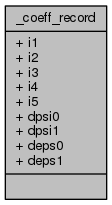
\includegraphics[width=171pt]{struct__coeff__record__coll__graph}
\end{center}
\end{figure}
\subsection*{\-Public \-Attributes}
\begin{DoxyCompactItemize}
\item 
int {\bf i1}
\item 
int {\bf i2}
\item 
int {\bf i3}
\item 
int {\bf i4}
\item 
int {\bf i5}
\item 
double {\bf dpsi0}
\item 
double {\bf dpsi1}
\item 
double {\bf deps0}
\item 
double {\bf deps1}
\end{DoxyCompactItemize}


\subsection{\-Detailed \-Description}


\-Definition at line 18 of file prenut.\-h.



\subsection{\-Member \-Data \-Documentation}
\index{\-\_\-coeff\-\_\-record@{\-\_\-coeff\-\_\-record}!deps0@{deps0}}
\index{deps0@{deps0}!_coeff_record@{\-\_\-coeff\-\_\-record}}
\subsubsection[{deps0}]{\setlength{\rightskip}{0pt plus 5cm}double {\bf \-\_\-coeff\-\_\-record\-::deps0}}\label{struct__coeff__record_acbe46502ed00c85951b61cece826cb68}


\-Definition at line 22 of file prenut.\-h.

\index{\-\_\-coeff\-\_\-record@{\-\_\-coeff\-\_\-record}!deps1@{deps1}}
\index{deps1@{deps1}!_coeff_record@{\-\_\-coeff\-\_\-record}}
\subsubsection[{deps1}]{\setlength{\rightskip}{0pt plus 5cm}double {\bf \-\_\-coeff\-\_\-record\-::deps1}}\label{struct__coeff__record_a6df09506dc331fb0af93719e691302b1}


\-Definition at line 22 of file prenut.\-h.

\index{\-\_\-coeff\-\_\-record@{\-\_\-coeff\-\_\-record}!dpsi0@{dpsi0}}
\index{dpsi0@{dpsi0}!_coeff_record@{\-\_\-coeff\-\_\-record}}
\subsubsection[{dpsi0}]{\setlength{\rightskip}{0pt plus 5cm}double {\bf \-\_\-coeff\-\_\-record\-::dpsi0}}\label{struct__coeff__record_ad7e3d2d5e8de00f3e69f714ab6e2f61d}


\-Definition at line 21 of file prenut.\-h.

\index{\-\_\-coeff\-\_\-record@{\-\_\-coeff\-\_\-record}!dpsi1@{dpsi1}}
\index{dpsi1@{dpsi1}!_coeff_record@{\-\_\-coeff\-\_\-record}}
\subsubsection[{dpsi1}]{\setlength{\rightskip}{0pt plus 5cm}double {\bf \-\_\-coeff\-\_\-record\-::dpsi1}}\label{struct__coeff__record_aaafae4c1b337d1a5f6a5248609e65645}


\-Definition at line 21 of file prenut.\-h.

\index{\-\_\-coeff\-\_\-record@{\-\_\-coeff\-\_\-record}!i1@{i1}}
\index{i1@{i1}!_coeff_record@{\-\_\-coeff\-\_\-record}}
\subsubsection[{i1}]{\setlength{\rightskip}{0pt plus 5cm}int {\bf \-\_\-coeff\-\_\-record\-::i1}}\label{struct__coeff__record_af26f8195abb73cea1b054aacf38781bc}


\-Definition at line 20 of file prenut.\-h.

\index{\-\_\-coeff\-\_\-record@{\-\_\-coeff\-\_\-record}!i2@{i2}}
\index{i2@{i2}!_coeff_record@{\-\_\-coeff\-\_\-record}}
\subsubsection[{i2}]{\setlength{\rightskip}{0pt plus 5cm}int {\bf \-\_\-coeff\-\_\-record\-::i2}}\label{struct__coeff__record_a9d3db03a7779e46f8afb83afc62538e8}


\-Definition at line 20 of file prenut.\-h.

\index{\-\_\-coeff\-\_\-record@{\-\_\-coeff\-\_\-record}!i3@{i3}}
\index{i3@{i3}!_coeff_record@{\-\_\-coeff\-\_\-record}}
\subsubsection[{i3}]{\setlength{\rightskip}{0pt plus 5cm}int {\bf \-\_\-coeff\-\_\-record\-::i3}}\label{struct__coeff__record_a5e5dde6efe7dad52d6e9c452ed61fd10}


\-Definition at line 20 of file prenut.\-h.

\index{\-\_\-coeff\-\_\-record@{\-\_\-coeff\-\_\-record}!i4@{i4}}
\index{i4@{i4}!_coeff_record@{\-\_\-coeff\-\_\-record}}
\subsubsection[{i4}]{\setlength{\rightskip}{0pt plus 5cm}int {\bf \-\_\-coeff\-\_\-record\-::i4}}\label{struct__coeff__record_a57bf69872dcd48023df1e9888c1a22e0}


\-Definition at line 20 of file prenut.\-h.

\index{\-\_\-coeff\-\_\-record@{\-\_\-coeff\-\_\-record}!i5@{i5}}
\index{i5@{i5}!_coeff_record@{\-\_\-coeff\-\_\-record}}
\subsubsection[{i5}]{\setlength{\rightskip}{0pt plus 5cm}int {\bf \-\_\-coeff\-\_\-record\-::i5}}\label{struct__coeff__record_aa556a03360f2703866ce6f3c63d2b6c2}


\-Definition at line 20 of file prenut.\-h.



\-The documentation for this struct was generated from the following file\-:\begin{DoxyCompactItemize}
\item 
\-Sist\-Referencia/{\bf prenut.\-h}\end{DoxyCompactItemize}

\input{class_c_d_m_1_1cdm_parser_1_1_c_d_m}
\section{\-Aplicacion.\-frm\-\_\-main.\-Conexion\-Norad \-Class \-Reference}
\label{class_aplicacion_1_1frm__main_1_1_conexion_norad}\index{\-Aplicacion.\-frm\-\_\-main.\-Conexion\-Norad@{\-Aplicacion.\-frm\-\_\-main.\-Conexion\-Norad}}


\-Inheritance diagram for \-Aplicacion.\-frm\-\_\-main.\-Conexion\-Norad\-:\nopagebreak
\begin{figure}[H]
\begin{center}
\leavevmode
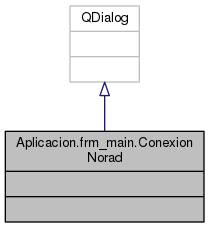
\includegraphics[width=254pt]{class_aplicacion_1_1frm__main_1_1_conexion_norad__inherit__graph}
\end{center}
\end{figure}


\-Collaboration diagram for \-Aplicacion.\-frm\-\_\-main.\-Conexion\-Norad\-:\nopagebreak
\begin{figure}[H]
\begin{center}
\leavevmode
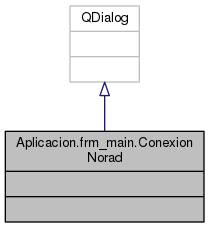
\includegraphics[width=254pt]{class_aplicacion_1_1frm__main_1_1_conexion_norad__coll__graph}
\end{center}
\end{figure}


\subsection{\-Detailed \-Description}


\-Definition at line 737 of file frm\-\_\-main.\-py.



\-The documentation for this class was generated from the following file\-:\begin{DoxyCompactItemize}
\item 
\-Aplicacion/{\bf frm\-\_\-main.\-py}\end{DoxyCompactItemize}

\section{pruebas.\-clase\-Tle.\-Encuentro \-Class \-Reference}
\label{classpruebas_1_1clase_tle_1_1_encuentro}\index{pruebas.\-clase\-Tle.\-Encuentro@{pruebas.\-clase\-Tle.\-Encuentro}}
\subsection*{\-Public \-Member \-Functions}
\begin{DoxyCompactItemize}
\item 
def {\bf \-\_\-\-\_\-init\-\_\-\-\_\-}
\end{DoxyCompactItemize}
\subsection*{\-Public \-Attributes}
\begin{DoxyCompactItemize}
\item 
{\bf tle\-\_\-sat}
\item 
{\bf tle\-\_\-deb}
\item 
{\bf tca}
\item 
{\bf \-Dist\-Ric}
\item 
{\bf archivo\-\_\-dif}
\item 
{\bf epoca\-\_\-ini}
\item 
{\bf mod\-\_\-min\-Dist}
\item 
{\bf \-Dist\-Vector}
\item 
{\bf \-Vel\-Vector}
\item 
{\bf mod\-\_\-\-Dist1}
\item 
{\bf tca\-\_\-c}
\item 
{\bf \-Dist\-Ric\-\_\-min}
\end{DoxyCompactItemize}


\subsection{\-Detailed \-Description}


\-Definition at line 147 of file clase\-Tle.\-py.



\subsection{\-Constructor \& \-Destructor \-Documentation}
\index{pruebas\-::clase\-Tle\-::\-Encuentro@{pruebas\-::clase\-Tle\-::\-Encuentro}!\-\_\-\-\_\-init\-\_\-\-\_\-@{\-\_\-\-\_\-init\-\_\-\-\_\-}}
\index{\-\_\-\-\_\-init\-\_\-\-\_\-@{\-\_\-\-\_\-init\-\_\-\-\_\-}!pruebas::claseTle::Encuentro@{pruebas\-::clase\-Tle\-::\-Encuentro}}
\subsubsection[{\-\_\-\-\_\-init\-\_\-\-\_\-}]{\setlength{\rightskip}{0pt plus 5cm}def {\bf pruebas.\-clase\-Tle.\-Encuentro.\-\_\-\-\_\-init\-\_\-\-\_\-} (
\begin{DoxyParamCaption}
\item[{}]{self, }
\item[{}]{tle\-\_\-sat, }
\item[{}]{tle\-\_\-deb, }
\item[{}]{tca}
\end{DoxyParamCaption}
)}\label{classpruebas_1_1clase_tle_1_1_encuentro_a7e6399999864f7f80bd1b9e4f3c4dee2}
\begin{DoxyVerb}
Calcula las diferencias en posiciones y velocidades 
para dos objetos en situacion de acercamiento, 5 minutos antes
y 5 minutos despues del tca.
-----------------------------------------------------------
outpus:
    3 archivos.
    mod_minDist: Minima distancia en modulo en el sistema RTN. (float)
    tca_c: Instante del maximo acercamiento. (datetime)
    DistRic_min: coordenadas RTN en el momento de min distancia (array)
\end{DoxyVerb}
 

\-Definition at line 149 of file clase\-Tle.\-py.


\begin{DoxyCode}
149 
150     def __init__(self,tle_sat,tle_deb,tca):
151         """
152         Calcula las diferencias en posiciones y velocidades 
153         para dos objetos en situacion de acercamiento, 5 minutos antes
154         y 5 minutos despues del tca.
155         -----------------------------------------------------------
156         outpus:
157             3 archivos.
158             mod_minDist: Minima distancia en modulo en el sistema RTN. (float)
159             tca_c: Instante del maximo acercamiento. (datetime)
160             DistRic_min: coordenadas RTN en el momento de min distancia (array)
161         """
162         
163         self.tle_sat=tle_sat
164         self.tle_deb=tle_deb
165         self.tca=tca
166         self.DistRic=0         
167         """
168         Genera Archivos
169         """
170         sat_id=self.tle_sat.catID()
171         deb_id=self.tle_deb.catID()
172         self.archivo_dif ='../Encuentro/archivos/'+str(sat_id)+'_'+str(deb_id)+
      '_rtn'
173         salida1=open('../Encuentro/archivos/'+str(sat_id),'w+')
174         salida2=open('../Encuentro/archivos/'+str(deb_id),'w+')
175         salida3=open(self.archivo_dif,'w+')
176 
177         """
178         Calcula las diferencias relativas entre los dos 
179         objetos en el sistema RTN.
180         """
181 
182         self.epoca_ini=self.tca-timedelta(minutes=5)
183         epoca_fin=self.tca+timedelta(minutes=5)
184         
185         self.mod_minDist=sys.float_info.max
186         while self.epoca_ini < epoca_fin:
187             r,v=self.tle_sat.propagaTLE(self.epoca_ini)
188             r1,v1=self.tle_deb.propagaTLE(self.epoca_ini)
189             
190             r=np.array([float(r[0]),float(r[1]),float(r[2])])
191             v=np.array([float(v[0]),float(v[1]),float(v[2])])
192             r1=np.array([float(r1[0]),float(r1[1]),float(r1[2])])
193             v1=np.array([float(v1[0]),float(v1[1]),float(v1[2])])
194             
195             pos1=Posicion(r,v,self.epoca_ini)
196             pos2=Posicion(r1,v1,self.epoca_ini)
197             
198             self.DistVector=pos1.r-pos2.r
199             x_ric,y_ric,z_ric=ricSis(pos1.r,pos1.v,self.DistVector)
200             self.DistRic=np.array([x_ric,y_ric,z_ric])
201             self.VelVector=pos1.v-pos2.v
202             self.mod_Dist1=np.sqrt(np.dot(self.DistRic,self.DistRic))
203 #            self.mod_Dist1=np.sqrt(np.dot(self.DistVector,self.DistVector))
204             if self.mod_Dist1 < self.mod_minDist:
205                 self.mod_minDist=self.mod_Dist1
206                 self.tca_c=self.epoca_ini
207                 self.DistRic_min=np.array([x_ric,y_ric,z_ric])
208             print self.epoca_ini, self.mod_Dist1
209             self.epoca_ini=self.epoca_ini+timedelta(seconds=1)
210             
211             # Transformo a Coordenadas Geodesicas.
212             delta1, alpha1=pos1.getCoordenadasGEOD()
213             delta2, alpha2=pos2.getCoordenadasGEOD()
214             # GUARDA EN ARCHIVO Posiciones en ALFA, DELTA (Seudo Geodesicas).
215             salida1.write(str(alpha1)+' '+str(delta1)+' '+datetime.strftime(
      pos1.epoca,'%Y-%m-%d %H:%M:%S')+'\n')
216             salida2.write(str(alpha2)+' '+str(delta2)+' '+datetime.strftime(
      pos2.epoca,'%Y-%m-%d %H:%M:%S')+'\n') 
217             # GUARDA EN ARCHIVO Posiciones en RTN.
218             salida3.write(datetime.strftime(pos1.epoca,'%Y-%m-%d %H:%M:%S')+' '
      +str(self.DistRic[0])+' '+str(self.DistRic[1])+' '+str(self.DistRic[2])+'\n')
219 
220         salida1.close()
221         salida2.close()
222         salida3.close()
223 
224 #     
225 # if __name__=='__main__':
226 #      
227 #      TCA=datetime(2008,1,9,19,0,30)
228 #      sat_id='27386' #ENVISAT
229 #      deb_id='15482' #COSMOS
230 #      usuario='macecilia'
231 #      clave='MaCeciliaSpace17'
232 #  
233 #      tle_sat=Tle(usuario,clave,sat_id,TCA)
234 #      tle_deb=Tle(usuario,clave,deb_id,TCA)
235 #      
236 #      encuentro1=Encuentro(tle_sat,tle_deb,TCA)
237 # #     dif_r,dif_v=encuentro1.svDif()
238 #     
239 #     tle_archivo=Tle.creadoxArchivo(archivo='../TleAdmin/tle/37673tle0')
240 #     print tle_archivo.epoca()
241     
    \end{DoxyCode}


\subsection{\-Member \-Data \-Documentation}
\index{pruebas\-::clase\-Tle\-::\-Encuentro@{pruebas\-::clase\-Tle\-::\-Encuentro}!archivo\-\_\-dif@{archivo\-\_\-dif}}
\index{archivo\-\_\-dif@{archivo\-\_\-dif}!pruebas::claseTle::Encuentro@{pruebas\-::clase\-Tle\-::\-Encuentro}}
\subsubsection[{archivo\-\_\-dif}]{\setlength{\rightskip}{0pt plus 5cm}{\bf pruebas\-::clase\-Tle.\-Encuentro\-::archivo\-\_\-dif}}\label{classpruebas_1_1clase_tle_1_1_encuentro_af72762abc3ab894e7ffc1e5424215eb3}


\-Definition at line 161 of file clase\-Tle.\-py.

\index{pruebas\-::clase\-Tle\-::\-Encuentro@{pruebas\-::clase\-Tle\-::\-Encuentro}!\-Dist\-Ric@{\-Dist\-Ric}}
\index{\-Dist\-Ric@{\-Dist\-Ric}!pruebas::claseTle::Encuentro@{pruebas\-::clase\-Tle\-::\-Encuentro}}
\subsubsection[{\-Dist\-Ric}]{\setlength{\rightskip}{0pt plus 5cm}{\bf pruebas\-::clase\-Tle.\-Encuentro\-::\-Dist\-Ric}}\label{classpruebas_1_1clase_tle_1_1_encuentro_a9580630b90329c0f138b47a47a4e993a}


\-Definition at line 159 of file clase\-Tle.\-py.

\index{pruebas\-::clase\-Tle\-::\-Encuentro@{pruebas\-::clase\-Tle\-::\-Encuentro}!\-Dist\-Ric\-\_\-min@{\-Dist\-Ric\-\_\-min}}
\index{\-Dist\-Ric\-\_\-min@{\-Dist\-Ric\-\_\-min}!pruebas::claseTle::Encuentro@{pruebas\-::clase\-Tle\-::\-Encuentro}}
\subsubsection[{\-Dist\-Ric\-\_\-min}]{\setlength{\rightskip}{0pt plus 5cm}{\bf pruebas\-::clase\-Tle.\-Encuentro\-::\-Dist\-Ric\-\_\-min}}\label{classpruebas_1_1clase_tle_1_1_encuentro_ada92cbea7ee81c5f5da61d08cb08acde}


\-Definition at line 164 of file clase\-Tle.\-py.

\index{pruebas\-::clase\-Tle\-::\-Encuentro@{pruebas\-::clase\-Tle\-::\-Encuentro}!\-Dist\-Vector@{\-Dist\-Vector}}
\index{\-Dist\-Vector@{\-Dist\-Vector}!pruebas::claseTle::Encuentro@{pruebas\-::clase\-Tle\-::\-Encuentro}}
\subsubsection[{\-Dist\-Vector}]{\setlength{\rightskip}{0pt plus 5cm}{\bf pruebas\-::clase\-Tle.\-Encuentro\-::\-Dist\-Vector}}\label{classpruebas_1_1clase_tle_1_1_encuentro_aedd8a3ee3330aff4d6aea7bd4c30c44b}


\-Definition at line 164 of file clase\-Tle.\-py.

\index{pruebas\-::clase\-Tle\-::\-Encuentro@{pruebas\-::clase\-Tle\-::\-Encuentro}!epoca\-\_\-ini@{epoca\-\_\-ini}}
\index{epoca\-\_\-ini@{epoca\-\_\-ini}!pruebas::claseTle::Encuentro@{pruebas\-::clase\-Tle\-::\-Encuentro}}
\subsubsection[{epoca\-\_\-ini}]{\setlength{\rightskip}{0pt plus 5cm}{\bf pruebas\-::clase\-Tle.\-Encuentro\-::epoca\-\_\-ini}}\label{classpruebas_1_1clase_tle_1_1_encuentro_a64cc6d8583bccb824569de3dda2efddb}


\-Definition at line 164 of file clase\-Tle.\-py.

\index{pruebas\-::clase\-Tle\-::\-Encuentro@{pruebas\-::clase\-Tle\-::\-Encuentro}!mod\-\_\-\-Dist1@{mod\-\_\-\-Dist1}}
\index{mod\-\_\-\-Dist1@{mod\-\_\-\-Dist1}!pruebas::claseTle::Encuentro@{pruebas\-::clase\-Tle\-::\-Encuentro}}
\subsubsection[{mod\-\_\-\-Dist1}]{\setlength{\rightskip}{0pt plus 5cm}{\bf pruebas\-::clase\-Tle.\-Encuentro\-::mod\-\_\-\-Dist1}}\label{classpruebas_1_1clase_tle_1_1_encuentro_a769750840e1f38038e22ace6a5a6bac7}


\-Definition at line 164 of file clase\-Tle.\-py.

\index{pruebas\-::clase\-Tle\-::\-Encuentro@{pruebas\-::clase\-Tle\-::\-Encuentro}!mod\-\_\-min\-Dist@{mod\-\_\-min\-Dist}}
\index{mod\-\_\-min\-Dist@{mod\-\_\-min\-Dist}!pruebas::claseTle::Encuentro@{pruebas\-::clase\-Tle\-::\-Encuentro}}
\subsubsection[{mod\-\_\-min\-Dist}]{\setlength{\rightskip}{0pt plus 5cm}{\bf pruebas\-::clase\-Tle.\-Encuentro\-::mod\-\_\-min\-Dist}}\label{classpruebas_1_1clase_tle_1_1_encuentro_ad2e2746fd37fe86d659b1c7e5731ba5a}


\-Definition at line 164 of file clase\-Tle.\-py.

\index{pruebas\-::clase\-Tle\-::\-Encuentro@{pruebas\-::clase\-Tle\-::\-Encuentro}!tca@{tca}}
\index{tca@{tca}!pruebas::claseTle::Encuentro@{pruebas\-::clase\-Tle\-::\-Encuentro}}
\subsubsection[{tca}]{\setlength{\rightskip}{0pt plus 5cm}{\bf pruebas\-::clase\-Tle.\-Encuentro\-::tca}}\label{classpruebas_1_1clase_tle_1_1_encuentro_a6517088d42ceaf01d97ccd1e2c8ccb5c}


\-Definition at line 159 of file clase\-Tle.\-py.

\index{pruebas\-::clase\-Tle\-::\-Encuentro@{pruebas\-::clase\-Tle\-::\-Encuentro}!tca\-\_\-c@{tca\-\_\-c}}
\index{tca\-\_\-c@{tca\-\_\-c}!pruebas::claseTle::Encuentro@{pruebas\-::clase\-Tle\-::\-Encuentro}}
\subsubsection[{tca\-\_\-c}]{\setlength{\rightskip}{0pt plus 5cm}{\bf pruebas\-::clase\-Tle.\-Encuentro\-::tca\-\_\-c}}\label{classpruebas_1_1clase_tle_1_1_encuentro_aafdda70a8d6f7862b4211f3a9fe49023}


\-Definition at line 164 of file clase\-Tle.\-py.

\index{pruebas\-::clase\-Tle\-::\-Encuentro@{pruebas\-::clase\-Tle\-::\-Encuentro}!tle\-\_\-deb@{tle\-\_\-deb}}
\index{tle\-\_\-deb@{tle\-\_\-deb}!pruebas::claseTle::Encuentro@{pruebas\-::clase\-Tle\-::\-Encuentro}}
\subsubsection[{tle\-\_\-deb}]{\setlength{\rightskip}{0pt plus 5cm}{\bf pruebas\-::clase\-Tle.\-Encuentro\-::tle\-\_\-deb}}\label{classpruebas_1_1clase_tle_1_1_encuentro_ad15cca3ff05d0048906d1d02140fbd7d}


\-Definition at line 159 of file clase\-Tle.\-py.

\index{pruebas\-::clase\-Tle\-::\-Encuentro@{pruebas\-::clase\-Tle\-::\-Encuentro}!tle\-\_\-sat@{tle\-\_\-sat}}
\index{tle\-\_\-sat@{tle\-\_\-sat}!pruebas::claseTle::Encuentro@{pruebas\-::clase\-Tle\-::\-Encuentro}}
\subsubsection[{tle\-\_\-sat}]{\setlength{\rightskip}{0pt plus 5cm}{\bf pruebas\-::clase\-Tle.\-Encuentro\-::tle\-\_\-sat}}\label{classpruebas_1_1clase_tle_1_1_encuentro_acde6947c44e857998bdb3f65b932f8d5}


\-Definition at line 159 of file clase\-Tle.\-py.

\index{pruebas\-::clase\-Tle\-::\-Encuentro@{pruebas\-::clase\-Tle\-::\-Encuentro}!\-Vel\-Vector@{\-Vel\-Vector}}
\index{\-Vel\-Vector@{\-Vel\-Vector}!pruebas::claseTle::Encuentro@{pruebas\-::clase\-Tle\-::\-Encuentro}}
\subsubsection[{\-Vel\-Vector}]{\setlength{\rightskip}{0pt plus 5cm}{\bf pruebas\-::clase\-Tle.\-Encuentro\-::\-Vel\-Vector}}\label{classpruebas_1_1clase_tle_1_1_encuentro_a592e3697e36b946c3945ab10110424df}


\-Definition at line 164 of file clase\-Tle.\-py.



\-The documentation for this class was generated from the following file\-:\begin{DoxyCompactItemize}
\item 
pruebas/{\bf clase\-Tle.\-py}\end{DoxyCompactItemize}

\input{class_encuentro_1_1_encuentro_1_1_encuentro}
\section{\-Cods\-Admin.\-Ephem\-C\-O\-D\-S.\-Ephem\-C\-O\-D\-S \-Class \-Reference}
\label{class_cods_admin_1_1_ephem_c_o_d_s_1_1_ephem_c_o_d_s}\index{\-Cods\-Admin.\-Ephem\-C\-O\-D\-S.\-Ephem\-C\-O\-D\-S@{\-Cods\-Admin.\-Ephem\-C\-O\-D\-S.\-Ephem\-C\-O\-D\-S}}
\subsection*{\-Public \-Member \-Functions}
\begin{DoxyCompactItemize}
\item 
def {\bf \-\_\-\-\_\-init\-\_\-\-\_\-}
\item 
def {\bf parsea\-\_\-epoca\-\_\-nombre}
\item 
def {\bf genera\-\_\-diccionario}
\end{DoxyCompactItemize}
\subsection*{\-Public \-Attributes}
\begin{DoxyCompactItemize}
\item 
{\bf nombre\-\_\-arch}
\item 
{\bf data}
\item 
{\bf anio}
\item 
{\bf mes}
\item 
{\bf dia}
\item 
{\bf hora}
\item 
{\bf minu}
\item 
{\bf seg}
\item 
{\bf epoca\-\_\-ephem}
\end{DoxyCompactItemize}


\subsection{\-Detailed \-Description}
\begin{DoxyVerb}
Facilita la manipulacion de los datos CODS.
\end{DoxyVerb}
 

\-Definition at line 9 of file \-Ephem\-C\-O\-D\-S.\-py.



\subsection{\-Constructor \& \-Destructor \-Documentation}
\index{\-Cods\-Admin\-::\-Ephem\-C\-O\-D\-S\-::\-Ephem\-C\-O\-D\-S@{\-Cods\-Admin\-::\-Ephem\-C\-O\-D\-S\-::\-Ephem\-C\-O\-D\-S}!\-\_\-\-\_\-init\-\_\-\-\_\-@{\-\_\-\-\_\-init\-\_\-\-\_\-}}
\index{\-\_\-\-\_\-init\-\_\-\-\_\-@{\-\_\-\-\_\-init\-\_\-\-\_\-}!CodsAdmin::EphemCODS::EphemCODS@{\-Cods\-Admin\-::\-Ephem\-C\-O\-D\-S\-::\-Ephem\-C\-O\-D\-S}}
\subsubsection[{\-\_\-\-\_\-init\-\_\-\-\_\-}]{\setlength{\rightskip}{0pt plus 5cm}def {\bf \-Cods\-Admin.\-Ephem\-C\-O\-D\-S.\-Ephem\-C\-O\-D\-S.\-\_\-\-\_\-init\-\_\-\-\_\-} (
\begin{DoxyParamCaption}
\item[{}]{self, }
\item[{}]{nombre\-\_\-archivo}
\end{DoxyParamCaption}
)}\label{class_cods_admin_1_1_ephem_c_o_d_s_1_1_ephem_c_o_d_s_a06e177a3091b9fcfa2c6d4c2322da657}
\begin{DoxyVerb}
Constructor
\end{DoxyVerb}
 

\-Definition at line 13 of file \-Ephem\-C\-O\-D\-S.\-py.


\begin{DoxyCode}
13 
14     def __init__(self, nombre_archivo):
15         '''
16         Constructor
17         '''
18         self.nombre_arch = nombre_archivo
19         self.data={}

\end{DoxyCode}


\subsection{\-Member \-Function \-Documentation}
\index{\-Cods\-Admin\-::\-Ephem\-C\-O\-D\-S\-::\-Ephem\-C\-O\-D\-S@{\-Cods\-Admin\-::\-Ephem\-C\-O\-D\-S\-::\-Ephem\-C\-O\-D\-S}!genera\-\_\-diccionario@{genera\-\_\-diccionario}}
\index{genera\-\_\-diccionario@{genera\-\_\-diccionario}!CodsAdmin::EphemCODS::EphemCODS@{\-Cods\-Admin\-::\-Ephem\-C\-O\-D\-S\-::\-Ephem\-C\-O\-D\-S}}
\subsubsection[{genera\-\_\-diccionario}]{\setlength{\rightskip}{0pt plus 5cm}def {\bf \-Cods\-Admin.\-Ephem\-C\-O\-D\-S.\-Ephem\-C\-O\-D\-S.\-genera\-\_\-diccionario} (
\begin{DoxyParamCaption}
\item[{}]{self}
\end{DoxyParamCaption}
)}\label{class_cods_admin_1_1_ephem_c_o_d_s_1_1_ephem_c_o_d_s_a0817365a5d6b142390fad1886de641a3}


\-Definition at line 31 of file \-Ephem\-C\-O\-D\-S.\-py.


\begin{DoxyCode}
31 
32     def genera_diccionario(self):
33         archivo=open(self.nombre_arch,'r')
34         contenido=archivo.readlines()
35         for c in contenido:
36             c1=c.split()           
37             if c1[0]=='*HEADER':
38                 continue
39             fecha=c[:26]
40             x=c1[2]
41             y=c1[3]
42             z=c1[4]
43             vx=c1[5]
44             vy=c1[6]
45             vz=c1[7]
46             self.epoca_ephem=datetime.strptime(fecha,'%Y/%m/%d %H:%M:%S.%f')
47             self.data[self.epoca_ephem]={'x':x,'y':y,'z':z,'vx':vx,'vy':vy,'vz'
      :vz}
48 
        return self.data
\end{DoxyCode}
\index{\-Cods\-Admin\-::\-Ephem\-C\-O\-D\-S\-::\-Ephem\-C\-O\-D\-S@{\-Cods\-Admin\-::\-Ephem\-C\-O\-D\-S\-::\-Ephem\-C\-O\-D\-S}!parsea\-\_\-epoca\-\_\-nombre@{parsea\-\_\-epoca\-\_\-nombre}}
\index{parsea\-\_\-epoca\-\_\-nombre@{parsea\-\_\-epoca\-\_\-nombre}!CodsAdmin::EphemCODS::EphemCODS@{\-Cods\-Admin\-::\-Ephem\-C\-O\-D\-S\-::\-Ephem\-C\-O\-D\-S}}
\subsubsection[{parsea\-\_\-epoca\-\_\-nombre}]{\setlength{\rightskip}{0pt plus 5cm}def {\bf \-Cods\-Admin.\-Ephem\-C\-O\-D\-S.\-Ephem\-C\-O\-D\-S.\-parsea\-\_\-epoca\-\_\-nombre} (
\begin{DoxyParamCaption}
\item[{}]{self}
\end{DoxyParamCaption}
)}\label{class_cods_admin_1_1_ephem_c_o_d_s_1_1_ephem_c_o_d_s_a45b17270534648ee350fa97e4841c36b}


\-Definition at line 20 of file \-Ephem\-C\-O\-D\-S.\-py.


\begin{DoxyCode}
20 
21     def parsea_epoca_nombre(self):
22         campos      = self.nombre_arch.split('_')
23         self.anio   = campos[1][0:4]
24         self.mes    = campos[1][4:6]
25         self.dia    = campos[1][6:8]
26         self.hora   = campos[2][0:2]
27         self.minu    = campos[2][2:4]
28         self.seg    = campos[2][4:6]
29         
30         return self.anio, self.mes, self.dia, self.hora, self.minu, self.seg
    
\end{DoxyCode}


\subsection{\-Member \-Data \-Documentation}
\index{\-Cods\-Admin\-::\-Ephem\-C\-O\-D\-S\-::\-Ephem\-C\-O\-D\-S@{\-Cods\-Admin\-::\-Ephem\-C\-O\-D\-S\-::\-Ephem\-C\-O\-D\-S}!anio@{anio}}
\index{anio@{anio}!CodsAdmin::EphemCODS::EphemCODS@{\-Cods\-Admin\-::\-Ephem\-C\-O\-D\-S\-::\-Ephem\-C\-O\-D\-S}}
\subsubsection[{anio}]{\setlength{\rightskip}{0pt plus 5cm}{\bf \-Cods\-Admin\-::\-Ephem\-C\-O\-D\-S.\-Ephem\-C\-O\-D\-S\-::anio}}\label{class_cods_admin_1_1_ephem_c_o_d_s_1_1_ephem_c_o_d_s_a1b08c1febcea122ce6cd27a4100c249f}


\-Definition at line 20 of file \-Ephem\-C\-O\-D\-S.\-py.

\index{\-Cods\-Admin\-::\-Ephem\-C\-O\-D\-S\-::\-Ephem\-C\-O\-D\-S@{\-Cods\-Admin\-::\-Ephem\-C\-O\-D\-S\-::\-Ephem\-C\-O\-D\-S}!data@{data}}
\index{data@{data}!CodsAdmin::EphemCODS::EphemCODS@{\-Cods\-Admin\-::\-Ephem\-C\-O\-D\-S\-::\-Ephem\-C\-O\-D\-S}}
\subsubsection[{data}]{\setlength{\rightskip}{0pt plus 5cm}{\bf \-Cods\-Admin\-::\-Ephem\-C\-O\-D\-S.\-Ephem\-C\-O\-D\-S\-::data}}\label{class_cods_admin_1_1_ephem_c_o_d_s_1_1_ephem_c_o_d_s_ab607b9aaf575cf2de6a5742c5f35838f}


\-Definition at line 15 of file \-Ephem\-C\-O\-D\-S.\-py.

\index{\-Cods\-Admin\-::\-Ephem\-C\-O\-D\-S\-::\-Ephem\-C\-O\-D\-S@{\-Cods\-Admin\-::\-Ephem\-C\-O\-D\-S\-::\-Ephem\-C\-O\-D\-S}!dia@{dia}}
\index{dia@{dia}!CodsAdmin::EphemCODS::EphemCODS@{\-Cods\-Admin\-::\-Ephem\-C\-O\-D\-S\-::\-Ephem\-C\-O\-D\-S}}
\subsubsection[{dia}]{\setlength{\rightskip}{0pt plus 5cm}{\bf \-Cods\-Admin\-::\-Ephem\-C\-O\-D\-S.\-Ephem\-C\-O\-D\-S\-::dia}}\label{class_cods_admin_1_1_ephem_c_o_d_s_1_1_ephem_c_o_d_s_aa8f3adf29ef617ea389ba811aac6a761}


\-Definition at line 20 of file \-Ephem\-C\-O\-D\-S.\-py.

\index{\-Cods\-Admin\-::\-Ephem\-C\-O\-D\-S\-::\-Ephem\-C\-O\-D\-S@{\-Cods\-Admin\-::\-Ephem\-C\-O\-D\-S\-::\-Ephem\-C\-O\-D\-S}!epoca\-\_\-ephem@{epoca\-\_\-ephem}}
\index{epoca\-\_\-ephem@{epoca\-\_\-ephem}!CodsAdmin::EphemCODS::EphemCODS@{\-Cods\-Admin\-::\-Ephem\-C\-O\-D\-S\-::\-Ephem\-C\-O\-D\-S}}
\subsubsection[{epoca\-\_\-ephem}]{\setlength{\rightskip}{0pt plus 5cm}{\bf \-Cods\-Admin\-::\-Ephem\-C\-O\-D\-S.\-Ephem\-C\-O\-D\-S\-::epoca\-\_\-ephem}}\label{class_cods_admin_1_1_ephem_c_o_d_s_1_1_ephem_c_o_d_s_a236275674569fbe2a1ec0db2979d6a95}


\-Definition at line 31 of file \-Ephem\-C\-O\-D\-S.\-py.

\index{\-Cods\-Admin\-::\-Ephem\-C\-O\-D\-S\-::\-Ephem\-C\-O\-D\-S@{\-Cods\-Admin\-::\-Ephem\-C\-O\-D\-S\-::\-Ephem\-C\-O\-D\-S}!hora@{hora}}
\index{hora@{hora}!CodsAdmin::EphemCODS::EphemCODS@{\-Cods\-Admin\-::\-Ephem\-C\-O\-D\-S\-::\-Ephem\-C\-O\-D\-S}}
\subsubsection[{hora}]{\setlength{\rightskip}{0pt plus 5cm}{\bf \-Cods\-Admin\-::\-Ephem\-C\-O\-D\-S.\-Ephem\-C\-O\-D\-S\-::hora}}\label{class_cods_admin_1_1_ephem_c_o_d_s_1_1_ephem_c_o_d_s_a11e554c8144973f26096993f8f409043}


\-Definition at line 20 of file \-Ephem\-C\-O\-D\-S.\-py.

\index{\-Cods\-Admin\-::\-Ephem\-C\-O\-D\-S\-::\-Ephem\-C\-O\-D\-S@{\-Cods\-Admin\-::\-Ephem\-C\-O\-D\-S\-::\-Ephem\-C\-O\-D\-S}!mes@{mes}}
\index{mes@{mes}!CodsAdmin::EphemCODS::EphemCODS@{\-Cods\-Admin\-::\-Ephem\-C\-O\-D\-S\-::\-Ephem\-C\-O\-D\-S}}
\subsubsection[{mes}]{\setlength{\rightskip}{0pt plus 5cm}{\bf \-Cods\-Admin\-::\-Ephem\-C\-O\-D\-S.\-Ephem\-C\-O\-D\-S\-::mes}}\label{class_cods_admin_1_1_ephem_c_o_d_s_1_1_ephem_c_o_d_s_a0d63d7655bbdfa9912799cc0e649b65f}


\-Definition at line 20 of file \-Ephem\-C\-O\-D\-S.\-py.

\index{\-Cods\-Admin\-::\-Ephem\-C\-O\-D\-S\-::\-Ephem\-C\-O\-D\-S@{\-Cods\-Admin\-::\-Ephem\-C\-O\-D\-S\-::\-Ephem\-C\-O\-D\-S}!minu@{minu}}
\index{minu@{minu}!CodsAdmin::EphemCODS::EphemCODS@{\-Cods\-Admin\-::\-Ephem\-C\-O\-D\-S\-::\-Ephem\-C\-O\-D\-S}}
\subsubsection[{minu}]{\setlength{\rightskip}{0pt plus 5cm}{\bf \-Cods\-Admin\-::\-Ephem\-C\-O\-D\-S.\-Ephem\-C\-O\-D\-S\-::minu}}\label{class_cods_admin_1_1_ephem_c_o_d_s_1_1_ephem_c_o_d_s_a0b6c86e2a071560855bf82117f883881}


\-Definition at line 20 of file \-Ephem\-C\-O\-D\-S.\-py.

\index{\-Cods\-Admin\-::\-Ephem\-C\-O\-D\-S\-::\-Ephem\-C\-O\-D\-S@{\-Cods\-Admin\-::\-Ephem\-C\-O\-D\-S\-::\-Ephem\-C\-O\-D\-S}!nombre\-\_\-arch@{nombre\-\_\-arch}}
\index{nombre\-\_\-arch@{nombre\-\_\-arch}!CodsAdmin::EphemCODS::EphemCODS@{\-Cods\-Admin\-::\-Ephem\-C\-O\-D\-S\-::\-Ephem\-C\-O\-D\-S}}
\subsubsection[{nombre\-\_\-arch}]{\setlength{\rightskip}{0pt plus 5cm}{\bf \-Cods\-Admin\-::\-Ephem\-C\-O\-D\-S.\-Ephem\-C\-O\-D\-S\-::nombre\-\_\-arch}}\label{class_cods_admin_1_1_ephem_c_o_d_s_1_1_ephem_c_o_d_s_ae01bd8c891aa0b84ba03c7100abd87d1}


\-Definition at line 15 of file \-Ephem\-C\-O\-D\-S.\-py.

\index{\-Cods\-Admin\-::\-Ephem\-C\-O\-D\-S\-::\-Ephem\-C\-O\-D\-S@{\-Cods\-Admin\-::\-Ephem\-C\-O\-D\-S\-::\-Ephem\-C\-O\-D\-S}!seg@{seg}}
\index{seg@{seg}!CodsAdmin::EphemCODS::EphemCODS@{\-Cods\-Admin\-::\-Ephem\-C\-O\-D\-S\-::\-Ephem\-C\-O\-D\-S}}
\subsubsection[{seg}]{\setlength{\rightskip}{0pt plus 5cm}{\bf \-Cods\-Admin\-::\-Ephem\-C\-O\-D\-S.\-Ephem\-C\-O\-D\-S\-::seg}}\label{class_cods_admin_1_1_ephem_c_o_d_s_1_1_ephem_c_o_d_s_a7e4a03710ca594e5f3aa864012f8af86}


\-Definition at line 20 of file \-Ephem\-C\-O\-D\-S.\-py.



\-The documentation for this class was generated from the following file\-:\begin{DoxyCompactItemize}
\item 
\-Cods\-Admin/{\bf \-Ephem\-C\-O\-D\-S.\-py}\end{DoxyCompactItemize}

\section{pruebas.\-P\-R\-U\-E\-B\-A2.\-Example \-Class \-Reference}
\label{classpruebas_1_1_p_r_u_e_b_a2_1_1_example}\index{pruebas.\-P\-R\-U\-E\-B\-A2.\-Example@{pruebas.\-P\-R\-U\-E\-B\-A2.\-Example}}
\subsection*{\-Public \-Member \-Functions}
\begin{DoxyCompactItemize}
\item 
def {\bf \-\_\-\-\_\-init\-\_\-\-\_\-}
\item 
def {\bf init\-U\-I}
\end{DoxyCompactItemize}
\subsection*{\-Public \-Attributes}
\begin{DoxyCompactItemize}
\item 
{\bf layout}
\item 
{\bf view\-And\-Table\-Layout}
\item 
{\bf dock\-View}
\item 
{\bf grview}
\item 
{\bf dock\-Table}
\item 
{\bf table}
\item 
{\bf list\-And\-Tree\-Layout}
\item 
{\bf dock\-List}
\item 
{\bf list}
\item 
{\bf dock\-Tree}
\item 
{\bf tree}
\end{DoxyCompactItemize}


\subsection{\-Detailed \-Description}


\-Definition at line 10 of file \-P\-R\-U\-E\-B\-A2.\-py.



\subsection{\-Constructor \& \-Destructor \-Documentation}
\index{pruebas\-::\-P\-R\-U\-E\-B\-A2\-::\-Example@{pruebas\-::\-P\-R\-U\-E\-B\-A2\-::\-Example}!\-\_\-\-\_\-init\-\_\-\-\_\-@{\-\_\-\-\_\-init\-\_\-\-\_\-}}
\index{\-\_\-\-\_\-init\-\_\-\-\_\-@{\-\_\-\-\_\-init\-\_\-\-\_\-}!pruebas::PRUEBA2::Example@{pruebas\-::\-P\-R\-U\-E\-B\-A2\-::\-Example}}
\subsubsection[{\-\_\-\-\_\-init\-\_\-\-\_\-}]{\setlength{\rightskip}{0pt plus 5cm}def {\bf pruebas.\-P\-R\-U\-E\-B\-A2.\-Example.\-\_\-\-\_\-init\-\_\-\-\_\-} (
\begin{DoxyParamCaption}
\item[{}]{self, }
\item[{}]{parent = {\ttfamily \-None}}
\end{DoxyParamCaption}
)}\label{classpruebas_1_1_p_r_u_e_b_a2_1_1_example_a054339ac7c8614489b28a903d1a0ab26}


\-Definition at line 11 of file \-P\-R\-U\-E\-B\-A2.\-py.


\begin{DoxyCode}
11 
12     def __init__(self, parent=None):
13         QWidget.__init__(self, parent)
14         self.layout = QVBoxLayout()
15         self.setLayout(self.layout)
16         self.initUI()      
 
\end{DoxyCode}


\subsection{\-Member \-Function \-Documentation}
\index{pruebas\-::\-P\-R\-U\-E\-B\-A2\-::\-Example@{pruebas\-::\-P\-R\-U\-E\-B\-A2\-::\-Example}!init\-U\-I@{init\-U\-I}}
\index{init\-U\-I@{init\-U\-I}!pruebas::PRUEBA2::Example@{pruebas\-::\-P\-R\-U\-E\-B\-A2\-::\-Example}}
\subsubsection[{init\-U\-I}]{\setlength{\rightskip}{0pt plus 5cm}def {\bf pruebas.\-P\-R\-U\-E\-B\-A2.\-Example.\-init\-U\-I} (
\begin{DoxyParamCaption}
\item[{}]{self}
\end{DoxyParamCaption}
)}\label{classpruebas_1_1_p_r_u_e_b_a2_1_1_example_a3b93d7949e430b851cee0717cc75f5a2}


\-Definition at line 17 of file \-P\-R\-U\-E\-B\-A2.\-py.


\begin{DoxyCode}
17 
18     def initUI(self):
19         self.viewAndTableLayout = QHBoxLayout()
20         self.dockView = QDockWidget("View")
21         self.grview = QGraphicsView(self.dockView)
22         self.dockView.setWidget(self.grview)
23         self.viewAndTableLayout.addWidget(self.dockView)
24  
25         self.dockTable = QDockWidget("Table")
26         self.table = QTableView()
27         self.dockTable.setWidget(self.table)
28         self.viewAndTableLayout.addWidget(self.dockTable)
29         self.layout.addLayout(self.viewAndTableLayout)
30  
31  
32         self.listAndTreeLayout = QHBoxLayout()
33         self.dockList = QDockWidget("List")
34         self.list = QListView()
35         self.dockList.setWidget(self.list)
36         self.listAndTreeLayout.addWidget(self.dockList)
37  
38         self.dockTree = QDockWidget("Tree")
39         self.tree = QTreeView()
40         self.listAndTreeLayout.addWidget(self.dockTree)
        self.layout.addLayout(self.listAndTreeLayout)
\end{DoxyCode}


\subsection{\-Member \-Data \-Documentation}
\index{pruebas\-::\-P\-R\-U\-E\-B\-A2\-::\-Example@{pruebas\-::\-P\-R\-U\-E\-B\-A2\-::\-Example}!dock\-List@{dock\-List}}
\index{dock\-List@{dock\-List}!pruebas::PRUEBA2::Example@{pruebas\-::\-P\-R\-U\-E\-B\-A2\-::\-Example}}
\subsubsection[{dock\-List}]{\setlength{\rightskip}{0pt plus 5cm}{\bf pruebas\-::\-P\-R\-U\-E\-B\-A2.\-Example\-::dock\-List}}\label{classpruebas_1_1_p_r_u_e_b_a2_1_1_example_aa105805e3a1fa5b65667547372fcaae3}


\-Definition at line 17 of file \-P\-R\-U\-E\-B\-A2.\-py.

\index{pruebas\-::\-P\-R\-U\-E\-B\-A2\-::\-Example@{pruebas\-::\-P\-R\-U\-E\-B\-A2\-::\-Example}!dock\-Table@{dock\-Table}}
\index{dock\-Table@{dock\-Table}!pruebas::PRUEBA2::Example@{pruebas\-::\-P\-R\-U\-E\-B\-A2\-::\-Example}}
\subsubsection[{dock\-Table}]{\setlength{\rightskip}{0pt plus 5cm}{\bf pruebas\-::\-P\-R\-U\-E\-B\-A2.\-Example\-::dock\-Table}}\label{classpruebas_1_1_p_r_u_e_b_a2_1_1_example_a75e7df632ddd95619832dec0d9e1ca69}


\-Definition at line 17 of file \-P\-R\-U\-E\-B\-A2.\-py.

\index{pruebas\-::\-P\-R\-U\-E\-B\-A2\-::\-Example@{pruebas\-::\-P\-R\-U\-E\-B\-A2\-::\-Example}!dock\-Tree@{dock\-Tree}}
\index{dock\-Tree@{dock\-Tree}!pruebas::PRUEBA2::Example@{pruebas\-::\-P\-R\-U\-E\-B\-A2\-::\-Example}}
\subsubsection[{dock\-Tree}]{\setlength{\rightskip}{0pt plus 5cm}{\bf pruebas\-::\-P\-R\-U\-E\-B\-A2.\-Example\-::dock\-Tree}}\label{classpruebas_1_1_p_r_u_e_b_a2_1_1_example_a2b6ea5e9d359dbf3b6f6c15ad521beb2}


\-Definition at line 17 of file \-P\-R\-U\-E\-B\-A2.\-py.

\index{pruebas\-::\-P\-R\-U\-E\-B\-A2\-::\-Example@{pruebas\-::\-P\-R\-U\-E\-B\-A2\-::\-Example}!dock\-View@{dock\-View}}
\index{dock\-View@{dock\-View}!pruebas::PRUEBA2::Example@{pruebas\-::\-P\-R\-U\-E\-B\-A2\-::\-Example}}
\subsubsection[{dock\-View}]{\setlength{\rightskip}{0pt plus 5cm}{\bf pruebas\-::\-P\-R\-U\-E\-B\-A2.\-Example\-::dock\-View}}\label{classpruebas_1_1_p_r_u_e_b_a2_1_1_example_a6c74c5ad792aaca37f0299f21d4d3822}


\-Definition at line 17 of file \-P\-R\-U\-E\-B\-A2.\-py.

\index{pruebas\-::\-P\-R\-U\-E\-B\-A2\-::\-Example@{pruebas\-::\-P\-R\-U\-E\-B\-A2\-::\-Example}!grview@{grview}}
\index{grview@{grview}!pruebas::PRUEBA2::Example@{pruebas\-::\-P\-R\-U\-E\-B\-A2\-::\-Example}}
\subsubsection[{grview}]{\setlength{\rightskip}{0pt plus 5cm}{\bf pruebas\-::\-P\-R\-U\-E\-B\-A2.\-Example\-::grview}}\label{classpruebas_1_1_p_r_u_e_b_a2_1_1_example_ab484c203281f75c171ac61a73008c8de}


\-Definition at line 17 of file \-P\-R\-U\-E\-B\-A2.\-py.

\index{pruebas\-::\-P\-R\-U\-E\-B\-A2\-::\-Example@{pruebas\-::\-P\-R\-U\-E\-B\-A2\-::\-Example}!layout@{layout}}
\index{layout@{layout}!pruebas::PRUEBA2::Example@{pruebas\-::\-P\-R\-U\-E\-B\-A2\-::\-Example}}
\subsubsection[{layout}]{\setlength{\rightskip}{0pt plus 5cm}{\bf pruebas\-::\-P\-R\-U\-E\-B\-A2.\-Example\-::layout}}\label{classpruebas_1_1_p_r_u_e_b_a2_1_1_example_ac78ea661374efc21127b55c07f959227}


\-Definition at line 11 of file \-P\-R\-U\-E\-B\-A2.\-py.

\index{pruebas\-::\-P\-R\-U\-E\-B\-A2\-::\-Example@{pruebas\-::\-P\-R\-U\-E\-B\-A2\-::\-Example}!list@{list}}
\index{list@{list}!pruebas::PRUEBA2::Example@{pruebas\-::\-P\-R\-U\-E\-B\-A2\-::\-Example}}
\subsubsection[{list}]{\setlength{\rightskip}{0pt plus 5cm}{\bf pruebas\-::\-P\-R\-U\-E\-B\-A2.\-Example\-::list}}\label{classpruebas_1_1_p_r_u_e_b_a2_1_1_example_a1d24349bb3bbcebee510b6fec83bf91e}


\-Definition at line 17 of file \-P\-R\-U\-E\-B\-A2.\-py.

\index{pruebas\-::\-P\-R\-U\-E\-B\-A2\-::\-Example@{pruebas\-::\-P\-R\-U\-E\-B\-A2\-::\-Example}!list\-And\-Tree\-Layout@{list\-And\-Tree\-Layout}}
\index{list\-And\-Tree\-Layout@{list\-And\-Tree\-Layout}!pruebas::PRUEBA2::Example@{pruebas\-::\-P\-R\-U\-E\-B\-A2\-::\-Example}}
\subsubsection[{list\-And\-Tree\-Layout}]{\setlength{\rightskip}{0pt plus 5cm}{\bf pruebas\-::\-P\-R\-U\-E\-B\-A2.\-Example\-::list\-And\-Tree\-Layout}}\label{classpruebas_1_1_p_r_u_e_b_a2_1_1_example_a7aec15ed10196ad201085064d9a3bc8a}


\-Definition at line 17 of file \-P\-R\-U\-E\-B\-A2.\-py.

\index{pruebas\-::\-P\-R\-U\-E\-B\-A2\-::\-Example@{pruebas\-::\-P\-R\-U\-E\-B\-A2\-::\-Example}!table@{table}}
\index{table@{table}!pruebas::PRUEBA2::Example@{pruebas\-::\-P\-R\-U\-E\-B\-A2\-::\-Example}}
\subsubsection[{table}]{\setlength{\rightskip}{0pt plus 5cm}{\bf pruebas\-::\-P\-R\-U\-E\-B\-A2.\-Example\-::table}}\label{classpruebas_1_1_p_r_u_e_b_a2_1_1_example_a5d65ff3d9c9c6a1fe5fe5ec416869e56}


\-Definition at line 17 of file \-P\-R\-U\-E\-B\-A2.\-py.

\index{pruebas\-::\-P\-R\-U\-E\-B\-A2\-::\-Example@{pruebas\-::\-P\-R\-U\-E\-B\-A2\-::\-Example}!tree@{tree}}
\index{tree@{tree}!pruebas::PRUEBA2::Example@{pruebas\-::\-P\-R\-U\-E\-B\-A2\-::\-Example}}
\subsubsection[{tree}]{\setlength{\rightskip}{0pt plus 5cm}{\bf pruebas\-::\-P\-R\-U\-E\-B\-A2.\-Example\-::tree}}\label{classpruebas_1_1_p_r_u_e_b_a2_1_1_example_ad318ad4264ddec31f117273b46592461}


\-Definition at line 17 of file \-P\-R\-U\-E\-B\-A2.\-py.

\index{pruebas\-::\-P\-R\-U\-E\-B\-A2\-::\-Example@{pruebas\-::\-P\-R\-U\-E\-B\-A2\-::\-Example}!view\-And\-Table\-Layout@{view\-And\-Table\-Layout}}
\index{view\-And\-Table\-Layout@{view\-And\-Table\-Layout}!pruebas::PRUEBA2::Example@{pruebas\-::\-P\-R\-U\-E\-B\-A2\-::\-Example}}
\subsubsection[{view\-And\-Table\-Layout}]{\setlength{\rightskip}{0pt plus 5cm}{\bf pruebas\-::\-P\-R\-U\-E\-B\-A2.\-Example\-::view\-And\-Table\-Layout}}\label{classpruebas_1_1_p_r_u_e_b_a2_1_1_example_a85d110eae750b892ccc31526a3c2ac22}


\-Definition at line 17 of file \-P\-R\-U\-E\-B\-A2.\-py.



\-The documentation for this class was generated from the following file\-:\begin{DoxyCompactItemize}
\item 
pruebas/{\bf \-P\-R\-U\-E\-B\-A2.\-py}\end{DoxyCompactItemize}

\section{\-Aplicacion\-C\-O\-D\-S.\-C\-O\-D\-Sinterface.\-Figura \-Class \-Reference}
\label{class_aplicacion_c_o_d_s_1_1_c_o_d_sinterface_1_1_figura}\index{\-Aplicacion\-C\-O\-D\-S.\-C\-O\-D\-Sinterface.\-Figura@{\-Aplicacion\-C\-O\-D\-S.\-C\-O\-D\-Sinterface.\-Figura}}


\-Inheritance diagram for \-Aplicacion\-C\-O\-D\-S.\-C\-O\-D\-Sinterface.\-Figura\-:\nopagebreak
\begin{figure}[H]
\begin{center}
\leavevmode
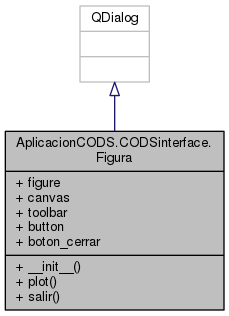
\includegraphics[width=270pt]{class_aplicacion_c_o_d_s_1_1_c_o_d_sinterface_1_1_figura__inherit__graph}
\end{center}
\end{figure}


\-Collaboration diagram for \-Aplicacion\-C\-O\-D\-S.\-C\-O\-D\-Sinterface.\-Figura\-:\nopagebreak
\begin{figure}[H]
\begin{center}
\leavevmode
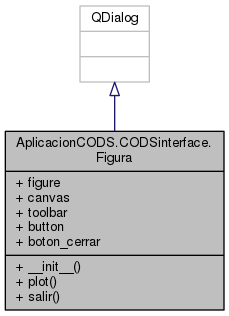
\includegraphics[width=270pt]{class_aplicacion_c_o_d_s_1_1_c_o_d_sinterface_1_1_figura__coll__graph}
\end{center}
\end{figure}
\subsection*{\-Public \-Member \-Functions}
\begin{DoxyCompactItemize}
\item 
def {\bf \-\_\-\-\_\-init\-\_\-\-\_\-}
\item 
def {\bf plot}
\item 
def {\bf salir}
\end{DoxyCompactItemize}
\subsection*{\-Public \-Attributes}
\begin{DoxyCompactItemize}
\item 
{\bf figure}
\item 
{\bf canvas}
\item 
{\bf toolbar}
\item 
{\bf button}
\item 
{\bf boton\-\_\-cerrar}
\end{DoxyCompactItemize}


\subsection{\-Detailed \-Description}


\-Definition at line 204 of file \-C\-O\-D\-Sinterface.\-py.



\subsection{\-Constructor \& \-Destructor \-Documentation}
\index{\-Aplicacion\-C\-O\-D\-S\-::\-C\-O\-D\-Sinterface\-::\-Figura@{\-Aplicacion\-C\-O\-D\-S\-::\-C\-O\-D\-Sinterface\-::\-Figura}!\-\_\-\-\_\-init\-\_\-\-\_\-@{\-\_\-\-\_\-init\-\_\-\-\_\-}}
\index{\-\_\-\-\_\-init\-\_\-\-\_\-@{\-\_\-\-\_\-init\-\_\-\-\_\-}!AplicacionCODS::CODSinterface::Figura@{\-Aplicacion\-C\-O\-D\-S\-::\-C\-O\-D\-Sinterface\-::\-Figura}}
\subsubsection[{\-\_\-\-\_\-init\-\_\-\-\_\-}]{\setlength{\rightskip}{0pt plus 5cm}def {\bf \-Aplicacion\-C\-O\-D\-S.\-C\-O\-D\-Sinterface.\-Figura.\-\_\-\-\_\-init\-\_\-\-\_\-} (
\begin{DoxyParamCaption}
\item[{}]{self, }
\item[{}]{parent = {\ttfamily \-None}}
\end{DoxyParamCaption}
)}\label{class_aplicacion_c_o_d_s_1_1_c_o_d_sinterface_1_1_figura_a3af94a94086672cc2d67a06813fc9079}


\-Definition at line 205 of file \-C\-O\-D\-Sinterface.\-py.


\begin{DoxyCode}
205 
206     def __init__(self, parent=None):
207         super(Figura, self).__init__(parent)
208         
209         # a figure instance to plot on
210         self.figure = plt.figure()
211 
212         # this is the Canvas Widget that displays the `figure`
213         self.canvas = FigureCanvas(self.figure)
214 
215         # this is the Navigation widget
216         self.toolbar = NavigationToolbar(self.canvas, self)
217 
218         # Just some button connected to `plot` method
219         self.button = QPushButton('Plot')
220         self.boton_cerrar=QPushButton('Cerrar')
221         self.button.clicked.connect(self.plot)
222         self.boton_cerrar.clicked.connect(self.salir)
223 
224         # set the layout
225         layout = QVBoxLayout()
226         layout.addWidget(self.toolbar)
227         layout.addWidget(self.canvas)
228         layout.addWidget(self.button)
229         layout.addWidget(self.boton_cerrar)
230         self.setLayout(layout)  
231 
     
\end{DoxyCode}


\subsection{\-Member \-Function \-Documentation}
\index{\-Aplicacion\-C\-O\-D\-S\-::\-C\-O\-D\-Sinterface\-::\-Figura@{\-Aplicacion\-C\-O\-D\-S\-::\-C\-O\-D\-Sinterface\-::\-Figura}!plot@{plot}}
\index{plot@{plot}!AplicacionCODS::CODSinterface::Figura@{\-Aplicacion\-C\-O\-D\-S\-::\-C\-O\-D\-Sinterface\-::\-Figura}}
\subsubsection[{plot}]{\setlength{\rightskip}{0pt plus 5cm}def {\bf \-Aplicacion\-C\-O\-D\-S.\-C\-O\-D\-Sinterface.\-Figura.\-plot} (
\begin{DoxyParamCaption}
\item[{}]{self}
\end{DoxyParamCaption}
)}\label{class_aplicacion_c_o_d_s_1_1_c_o_d_sinterface_1_1_figura_a0d671d42c702450e2f2a7f2bb6264487}


\-Definition at line 232 of file \-C\-O\-D\-Sinterface.\-py.


\begin{DoxyCode}
232 
233     def plot(self):
234         f=open('../main/codsOsweiler.dif','r')
235         listas=f.readlines()
236     
237         data0=[]
238         data1=[]
239         data2=[]
240         data3=[]
241         
242         for l in listas:
243             linea=l.split(' ')
244             data0.append(linea[0])
245             data1.append(float(linea[2]))
246             data2.append(float(linea[3]))
247             data3.append(float(linea[4]))
248 
249         """
250         Gestion de Fechas
251         """
252         date_fmt = '%Y-%m-%d'
253         epoca=[dt.datetime.strptime(str(i), date_fmt) for i in data0]
254         x = [mdates.date2num(i) for i in epoca]
255         date_formatter = mdates.DateFormatter('%d-%m-%y')
256     
257         # create an axis
258         ax1 = self.figure.add_subplot(311) 
259         ax2 = self.figure.add_subplot(312) 
260         ax3 = self.figure.add_subplot(313) 
261         ax1.xaxis.set_major_formatter(date_formatter)
262         ax2.xaxis.set_major_formatter(date_formatter)
263         ax3.xaxis.set_major_formatter(date_formatter)
264         ax1.grid(True)
265         ax2.grid(True)
266         ax3.grid(True)
267         
268         # discards the old graph
269         #ax.hold(False)
270         
271         # plot data
272         ax1.plot_date(x, data1,'x')
273         ax2.plot_date(x, data2,'x')
274         ax3.plot_date(x, data3,'x')
275 
276         # refresh canvas
277         self.canvas.draw() 
        
\end{DoxyCode}
\index{\-Aplicacion\-C\-O\-D\-S\-::\-C\-O\-D\-Sinterface\-::\-Figura@{\-Aplicacion\-C\-O\-D\-S\-::\-C\-O\-D\-Sinterface\-::\-Figura}!salir@{salir}}
\index{salir@{salir}!AplicacionCODS::CODSinterface::Figura@{\-Aplicacion\-C\-O\-D\-S\-::\-C\-O\-D\-Sinterface\-::\-Figura}}
\subsubsection[{salir}]{\setlength{\rightskip}{0pt plus 5cm}def {\bf \-Aplicacion\-C\-O\-D\-S.\-C\-O\-D\-Sinterface.\-Figura.\-salir} (
\begin{DoxyParamCaption}
\item[{}]{self}
\end{DoxyParamCaption}
)}\label{class_aplicacion_c_o_d_s_1_1_c_o_d_sinterface_1_1_figura_a448f006ff4bad5a28c2eb099a8b47de8}


\-Definition at line 278 of file \-C\-O\-D\-Sinterface.\-py.


\begin{DoxyCode}
278 
279     def salir(self):
        self.close()
\end{DoxyCode}


\subsection{\-Member \-Data \-Documentation}
\index{\-Aplicacion\-C\-O\-D\-S\-::\-C\-O\-D\-Sinterface\-::\-Figura@{\-Aplicacion\-C\-O\-D\-S\-::\-C\-O\-D\-Sinterface\-::\-Figura}!boton\-\_\-cerrar@{boton\-\_\-cerrar}}
\index{boton\-\_\-cerrar@{boton\-\_\-cerrar}!AplicacionCODS::CODSinterface::Figura@{\-Aplicacion\-C\-O\-D\-S\-::\-C\-O\-D\-Sinterface\-::\-Figura}}
\subsubsection[{boton\-\_\-cerrar}]{\setlength{\rightskip}{0pt plus 5cm}{\bf \-Aplicacion\-C\-O\-D\-S\-::\-C\-O\-D\-Sinterface.\-Figura\-::boton\-\_\-cerrar}}\label{class_aplicacion_c_o_d_s_1_1_c_o_d_sinterface_1_1_figura_a35eafa553dffeeff2892550c3ae58c14}


\-Definition at line 205 of file \-C\-O\-D\-Sinterface.\-py.

\index{\-Aplicacion\-C\-O\-D\-S\-::\-C\-O\-D\-Sinterface\-::\-Figura@{\-Aplicacion\-C\-O\-D\-S\-::\-C\-O\-D\-Sinterface\-::\-Figura}!button@{button}}
\index{button@{button}!AplicacionCODS::CODSinterface::Figura@{\-Aplicacion\-C\-O\-D\-S\-::\-C\-O\-D\-Sinterface\-::\-Figura}}
\subsubsection[{button}]{\setlength{\rightskip}{0pt plus 5cm}{\bf \-Aplicacion\-C\-O\-D\-S\-::\-C\-O\-D\-Sinterface.\-Figura\-::button}}\label{class_aplicacion_c_o_d_s_1_1_c_o_d_sinterface_1_1_figura_ae98c6618eac6902cd88d1b7d482bee4f}


\-Definition at line 205 of file \-C\-O\-D\-Sinterface.\-py.

\index{\-Aplicacion\-C\-O\-D\-S\-::\-C\-O\-D\-Sinterface\-::\-Figura@{\-Aplicacion\-C\-O\-D\-S\-::\-C\-O\-D\-Sinterface\-::\-Figura}!canvas@{canvas}}
\index{canvas@{canvas}!AplicacionCODS::CODSinterface::Figura@{\-Aplicacion\-C\-O\-D\-S\-::\-C\-O\-D\-Sinterface\-::\-Figura}}
\subsubsection[{canvas}]{\setlength{\rightskip}{0pt plus 5cm}{\bf \-Aplicacion\-C\-O\-D\-S\-::\-C\-O\-D\-Sinterface.\-Figura\-::canvas}}\label{class_aplicacion_c_o_d_s_1_1_c_o_d_sinterface_1_1_figura_ab992145611364acb282e156da020dbfa}


\-Definition at line 205 of file \-C\-O\-D\-Sinterface.\-py.

\index{\-Aplicacion\-C\-O\-D\-S\-::\-C\-O\-D\-Sinterface\-::\-Figura@{\-Aplicacion\-C\-O\-D\-S\-::\-C\-O\-D\-Sinterface\-::\-Figura}!figure@{figure}}
\index{figure@{figure}!AplicacionCODS::CODSinterface::Figura@{\-Aplicacion\-C\-O\-D\-S\-::\-C\-O\-D\-Sinterface\-::\-Figura}}
\subsubsection[{figure}]{\setlength{\rightskip}{0pt plus 5cm}{\bf \-Aplicacion\-C\-O\-D\-S\-::\-C\-O\-D\-Sinterface.\-Figura\-::figure}}\label{class_aplicacion_c_o_d_s_1_1_c_o_d_sinterface_1_1_figura_ae76c81e26aa4460f5a8ef274dc0f53b4}


\-Definition at line 205 of file \-C\-O\-D\-Sinterface.\-py.

\index{\-Aplicacion\-C\-O\-D\-S\-::\-C\-O\-D\-Sinterface\-::\-Figura@{\-Aplicacion\-C\-O\-D\-S\-::\-C\-O\-D\-Sinterface\-::\-Figura}!toolbar@{toolbar}}
\index{toolbar@{toolbar}!AplicacionCODS::CODSinterface::Figura@{\-Aplicacion\-C\-O\-D\-S\-::\-C\-O\-D\-Sinterface\-::\-Figura}}
\subsubsection[{toolbar}]{\setlength{\rightskip}{0pt plus 5cm}{\bf \-Aplicacion\-C\-O\-D\-S\-::\-C\-O\-D\-Sinterface.\-Figura\-::toolbar}}\label{class_aplicacion_c_o_d_s_1_1_c_o_d_sinterface_1_1_figura_aa23f26f0a0a76afc16f7568ad5444e32}


\-Definition at line 205 of file \-C\-O\-D\-Sinterface.\-py.



\-The documentation for this class was generated from the following file\-:\begin{DoxyCompactItemize}
\item 
\-Aplicacion\-C\-O\-D\-S/{\bf \-C\-O\-D\-Sinterface.\-py}\end{DoxyCompactItemize}

\input{class_tle_admin_1_1get__tle_1_1importar_set_t_l_e}
\section{pruebas.\-ejemplo.\-Main\-Window \-Class \-Reference}
\label{classpruebas_1_1ejemplo_1_1_main_window}\index{pruebas.\-ejemplo.\-Main\-Window@{pruebas.\-ejemplo.\-Main\-Window}}
\subsection*{\-Public \-Member \-Functions}
\begin{DoxyCompactItemize}
\item 
def {\bf \-\_\-\-\_\-init\-\_\-\-\_\-}
\item 
def {\bf update\-\_\-progress}
\item 
def {\bf hide\-\_\-progress\-\_\-bar}
\item 
def {\bf about}
\item 
def {\bf create\-Actions}
\item 
def {\bf create\-Menus}
\item 
def {\bf create\-Status\-Bar}
\end{DoxyCompactItemize}
\subsection*{\-Public \-Attributes}
\begin{DoxyCompactItemize}
\item 
{\bf rw}
\item 
{\bf sw}
\item 
{\bf pb}
\item 
{\bf exit\-Act}
\item 
{\bf about\-Act}
\item 
{\bf about\-Qt\-Act}
\item 
{\bf file\-Menu}
\item 
{\bf help\-Menu}
\end{DoxyCompactItemize}


\subsection{\-Detailed \-Description}


\-Definition at line 20 of file ejemplo.\-py.



\subsection{\-Constructor \& \-Destructor \-Documentation}
\index{pruebas\-::ejemplo\-::\-Main\-Window@{pruebas\-::ejemplo\-::\-Main\-Window}!\-\_\-\-\_\-init\-\_\-\-\_\-@{\-\_\-\-\_\-init\-\_\-\-\_\-}}
\index{\-\_\-\-\_\-init\-\_\-\-\_\-@{\-\_\-\-\_\-init\-\_\-\-\_\-}!pruebas::ejemplo::MainWindow@{pruebas\-::ejemplo\-::\-Main\-Window}}
\subsubsection[{\-\_\-\-\_\-init\-\_\-\-\_\-}]{\setlength{\rightskip}{0pt plus 5cm}def {\bf pruebas.\-ejemplo.\-Main\-Window.\-\_\-\-\_\-init\-\_\-\-\_\-} (
\begin{DoxyParamCaption}
\item[{}]{self}
\end{DoxyParamCaption}
)}\label{classpruebas_1_1ejemplo_1_1_main_window_a8acbdeaed4b6aa1ca5c6091d036fb4c7}


\-Definition at line 21 of file ejemplo.\-py.


\begin{DoxyCode}
21 
22     def __init__(self):
23         QMainWindow.__init__(self)
24 
25         # create stuff
26         self.rw = ReportWidget()
27         self.setCentralWidget(self.rw)
28         self.sw = StartWindow()
29         self.createActions()
30         self.createMenus()
31         self.createStatusBar()
32 
33         # create progress bar
34         self.pb = QProgressBar(self.statusBar())
35         self.statusBar().addPermanentWidget(self.pb)
36 
37         # connections
38         self.connect(self.sw, SIGNAL("okClicked"),
39                     self.rw.create)
40         self.connect(self.rw.table, SIGNAL("progressChanged"),
41                      self.update_progress)
42         self.connect(self.rw.table, SIGNAL("displayFinished"),
43                      self.hide_progress_bar)
44 
45         # format the main window
46         self.setGeometry(100,100,750,550)
47 
48         # show windows
49         self.show()
50         self.sw.show()

\end{DoxyCode}


\subsection{\-Member \-Function \-Documentation}
\index{pruebas\-::ejemplo\-::\-Main\-Window@{pruebas\-::ejemplo\-::\-Main\-Window}!about@{about}}
\index{about@{about}!pruebas::ejemplo::MainWindow@{pruebas\-::ejemplo\-::\-Main\-Window}}
\subsubsection[{about}]{\setlength{\rightskip}{0pt plus 5cm}def {\bf pruebas.\-ejemplo.\-Main\-Window.\-about} (
\begin{DoxyParamCaption}
\item[{}]{self}
\end{DoxyParamCaption}
)}\label{classpruebas_1_1ejemplo_1_1_main_window_a37c42bc9e0c1a391dd1380a87001ec44}


\-Definition at line 61 of file ejemplo.\-py.


\begin{DoxyCode}
61 
62     def about(self):
63         QMessageBox.about(self, self.tr("About AIS Audit Tool"),
64             self.tr("AIS Audit Tool\n\n"
65                     "%s\n"
66                     "%s\n"
67                     "%s" % (__author__, __version__, __date__)))

\end{DoxyCode}
\index{pruebas\-::ejemplo\-::\-Main\-Window@{pruebas\-::ejemplo\-::\-Main\-Window}!create\-Actions@{create\-Actions}}
\index{create\-Actions@{create\-Actions}!pruebas::ejemplo::MainWindow@{pruebas\-::ejemplo\-::\-Main\-Window}}
\subsubsection[{create\-Actions}]{\setlength{\rightskip}{0pt plus 5cm}def {\bf pruebas.\-ejemplo.\-Main\-Window.\-create\-Actions} (
\begin{DoxyParamCaption}
\item[{}]{self}
\end{DoxyParamCaption}
)}\label{classpruebas_1_1ejemplo_1_1_main_window_a0523db8099327476d11b1baad0d1d884}


\-Definition at line 68 of file ejemplo.\-py.


\begin{DoxyCode}
68 
69     def createActions(self):
70         self.exitAct = QAction(self.tr("E&xit;"), self)
71         self.exitAct.setShortcut(self.tr("Ctrl+Q"))
72         self.exitAct.setStatusTip(self.tr("Exit the application"))
73         self.connect(self.exitAct, SIGNAL("triggered()"), self, SLOT("close()")
      )
74 
75         self.aboutAct = QAction(self.tr("&About;"), self)
76         self.aboutAct.setStatusTip(self.tr("Show the application's About box"))
77         self.connect(self.aboutAct, SIGNAL("triggered()"), self.about)
78 
79         self.aboutQtAct = QAction(self.tr("About &Qt;"), self)
80         self.aboutQtAct.setStatusTip(self.tr("Show the Qt library's About box")
      )
81         self.connect(self.aboutQtAct, SIGNAL("triggered()"), qApp, SLOT("
      aboutQt()"))

\end{DoxyCode}
\index{pruebas\-::ejemplo\-::\-Main\-Window@{pruebas\-::ejemplo\-::\-Main\-Window}!create\-Menus@{create\-Menus}}
\index{create\-Menus@{create\-Menus}!pruebas::ejemplo::MainWindow@{pruebas\-::ejemplo\-::\-Main\-Window}}
\subsubsection[{create\-Menus}]{\setlength{\rightskip}{0pt plus 5cm}def {\bf pruebas.\-ejemplo.\-Main\-Window.\-create\-Menus} (
\begin{DoxyParamCaption}
\item[{}]{self}
\end{DoxyParamCaption}
)}\label{classpruebas_1_1ejemplo_1_1_main_window_a5bffdcee22936064b738b7bd5c5d12e9}


\-Definition at line 82 of file ejemplo.\-py.


\begin{DoxyCode}
82 
83     def createMenus(self):
84         self.fileMenu = self.menuBar().addMenu(self.tr("&File;"))
85         self.fileMenu.addAction(self.exitAct)
86 
87         self.helpMenu = self.menuBar().addMenu(self.tr("&Help;"))
88         self.helpMenu.addAction(self.aboutAct)
89         self.helpMenu.addAction(self.aboutQtAct)

\end{DoxyCode}
\index{pruebas\-::ejemplo\-::\-Main\-Window@{pruebas\-::ejemplo\-::\-Main\-Window}!create\-Status\-Bar@{create\-Status\-Bar}}
\index{create\-Status\-Bar@{create\-Status\-Bar}!pruebas::ejemplo::MainWindow@{pruebas\-::ejemplo\-::\-Main\-Window}}
\subsubsection[{create\-Status\-Bar}]{\setlength{\rightskip}{0pt plus 5cm}def {\bf pruebas.\-ejemplo.\-Main\-Window.\-create\-Status\-Bar} (
\begin{DoxyParamCaption}
\item[{}]{self}
\end{DoxyParamCaption}
)}\label{classpruebas_1_1ejemplo_1_1_main_window_ade11ed356e510750c282dc2d626211f1}


\-Definition at line 90 of file ejemplo.\-py.


\begin{DoxyCode}
90 
91     def createStatusBar(self):
92         sb = QStatusBar()
93         sb.setFixedHeight(18)
94         self.setStatusBar(sb)
95         self.statusBar().showMessage(self.tr("Ready"))

\end{DoxyCode}
\index{pruebas\-::ejemplo\-::\-Main\-Window@{pruebas\-::ejemplo\-::\-Main\-Window}!hide\-\_\-progress\-\_\-bar@{hide\-\_\-progress\-\_\-bar}}
\index{hide\-\_\-progress\-\_\-bar@{hide\-\_\-progress\-\_\-bar}!pruebas::ejemplo::MainWindow@{pruebas\-::ejemplo\-::\-Main\-Window}}
\subsubsection[{hide\-\_\-progress\-\_\-bar}]{\setlength{\rightskip}{0pt plus 5cm}def {\bf pruebas.\-ejemplo.\-Main\-Window.\-hide\-\_\-progress\-\_\-bar} (
\begin{DoxyParamCaption}
\item[{}]{self}
\end{DoxyParamCaption}
)}\label{classpruebas_1_1ejemplo_1_1_main_window_adbd6705630409563ff24cb24736b8161}


\-Definition at line 57 of file ejemplo.\-py.


\begin{DoxyCode}
57 
58     def hide_progress_bar(self):
59         self.pb.hide()
60         self.statusBar().showMessage(self.tr("Finished"))

\end{DoxyCode}
\index{pruebas\-::ejemplo\-::\-Main\-Window@{pruebas\-::ejemplo\-::\-Main\-Window}!update\-\_\-progress@{update\-\_\-progress}}
\index{update\-\_\-progress@{update\-\_\-progress}!pruebas::ejemplo::MainWindow@{pruebas\-::ejemplo\-::\-Main\-Window}}
\subsubsection[{update\-\_\-progress}]{\setlength{\rightskip}{0pt plus 5cm}def {\bf pruebas.\-ejemplo.\-Main\-Window.\-update\-\_\-progress} (
\begin{DoxyParamCaption}
\item[{}]{self, }
\item[{}]{n, }
\item[{}]{nrows}
\end{DoxyParamCaption}
)}\label{classpruebas_1_1ejemplo_1_1_main_window_a62d2740c793ed405ce211128b9959b19}


\-Definition at line 51 of file ejemplo.\-py.


\begin{DoxyCode}
51 
52     def update_progress(self, n, nrows):
53         self.pb.show()
54         self.pb.setRange(0, nrows)
55         self.pb.setValue(n)
56         self.statusBar().showMessage(self.tr("Parsing eventlog data..."))

\end{DoxyCode}


\subsection{\-Member \-Data \-Documentation}
\index{pruebas\-::ejemplo\-::\-Main\-Window@{pruebas\-::ejemplo\-::\-Main\-Window}!about\-Act@{about\-Act}}
\index{about\-Act@{about\-Act}!pruebas::ejemplo::MainWindow@{pruebas\-::ejemplo\-::\-Main\-Window}}
\subsubsection[{about\-Act}]{\setlength{\rightskip}{0pt plus 5cm}{\bf pruebas\-::ejemplo.\-Main\-Window\-::about\-Act}}\label{classpruebas_1_1ejemplo_1_1_main_window_af8a4c14582c3669ce696fd7bac89f3b6}


\-Definition at line 68 of file ejemplo.\-py.

\index{pruebas\-::ejemplo\-::\-Main\-Window@{pruebas\-::ejemplo\-::\-Main\-Window}!about\-Qt\-Act@{about\-Qt\-Act}}
\index{about\-Qt\-Act@{about\-Qt\-Act}!pruebas::ejemplo::MainWindow@{pruebas\-::ejemplo\-::\-Main\-Window}}
\subsubsection[{about\-Qt\-Act}]{\setlength{\rightskip}{0pt plus 5cm}{\bf pruebas\-::ejemplo.\-Main\-Window\-::about\-Qt\-Act}}\label{classpruebas_1_1ejemplo_1_1_main_window_a8d95064b621622fbea64d10d1cea0dcf}


\-Definition at line 68 of file ejemplo.\-py.

\index{pruebas\-::ejemplo\-::\-Main\-Window@{pruebas\-::ejemplo\-::\-Main\-Window}!exit\-Act@{exit\-Act}}
\index{exit\-Act@{exit\-Act}!pruebas::ejemplo::MainWindow@{pruebas\-::ejemplo\-::\-Main\-Window}}
\subsubsection[{exit\-Act}]{\setlength{\rightskip}{0pt plus 5cm}{\bf pruebas\-::ejemplo.\-Main\-Window\-::exit\-Act}}\label{classpruebas_1_1ejemplo_1_1_main_window_ac908ffbb4c1b2b4fcbb913c06c290f33}


\-Definition at line 68 of file ejemplo.\-py.

\index{pruebas\-::ejemplo\-::\-Main\-Window@{pruebas\-::ejemplo\-::\-Main\-Window}!file\-Menu@{file\-Menu}}
\index{file\-Menu@{file\-Menu}!pruebas::ejemplo::MainWindow@{pruebas\-::ejemplo\-::\-Main\-Window}}
\subsubsection[{file\-Menu}]{\setlength{\rightskip}{0pt plus 5cm}{\bf pruebas\-::ejemplo.\-Main\-Window\-::file\-Menu}}\label{classpruebas_1_1ejemplo_1_1_main_window_a93177a92313d6cc95421f999e43db74c}


\-Definition at line 82 of file ejemplo.\-py.

\index{pruebas\-::ejemplo\-::\-Main\-Window@{pruebas\-::ejemplo\-::\-Main\-Window}!help\-Menu@{help\-Menu}}
\index{help\-Menu@{help\-Menu}!pruebas::ejemplo::MainWindow@{pruebas\-::ejemplo\-::\-Main\-Window}}
\subsubsection[{help\-Menu}]{\setlength{\rightskip}{0pt plus 5cm}{\bf pruebas\-::ejemplo.\-Main\-Window\-::help\-Menu}}\label{classpruebas_1_1ejemplo_1_1_main_window_a9eefde030194eada361f6fd952c2b349}


\-Definition at line 82 of file ejemplo.\-py.

\index{pruebas\-::ejemplo\-::\-Main\-Window@{pruebas\-::ejemplo\-::\-Main\-Window}!pb@{pb}}
\index{pb@{pb}!pruebas::ejemplo::MainWindow@{pruebas\-::ejemplo\-::\-Main\-Window}}
\subsubsection[{pb}]{\setlength{\rightskip}{0pt plus 5cm}{\bf pruebas\-::ejemplo.\-Main\-Window\-::pb}}\label{classpruebas_1_1ejemplo_1_1_main_window_a71243d6087f172789ed631596a83eb50}


\-Definition at line 21 of file ejemplo.\-py.

\index{pruebas\-::ejemplo\-::\-Main\-Window@{pruebas\-::ejemplo\-::\-Main\-Window}!rw@{rw}}
\index{rw@{rw}!pruebas::ejemplo::MainWindow@{pruebas\-::ejemplo\-::\-Main\-Window}}
\subsubsection[{rw}]{\setlength{\rightskip}{0pt plus 5cm}{\bf pruebas\-::ejemplo.\-Main\-Window\-::rw}}\label{classpruebas_1_1ejemplo_1_1_main_window_a0b0d91293dbd8eb6ddbd99789b2d3c16}


\-Definition at line 21 of file ejemplo.\-py.

\index{pruebas\-::ejemplo\-::\-Main\-Window@{pruebas\-::ejemplo\-::\-Main\-Window}!sw@{sw}}
\index{sw@{sw}!pruebas::ejemplo::MainWindow@{pruebas\-::ejemplo\-::\-Main\-Window}}
\subsubsection[{sw}]{\setlength{\rightskip}{0pt plus 5cm}{\bf pruebas\-::ejemplo.\-Main\-Window\-::sw}}\label{classpruebas_1_1ejemplo_1_1_main_window_adaeb2bbf0b2eb94c9300b7eae7c8a60e}


\-Definition at line 21 of file ejemplo.\-py.



\-The documentation for this class was generated from the following file\-:\begin{DoxyCompactItemize}
\item 
pruebas/{\bf ejemplo.\-py}\end{DoxyCompactItemize}

\section{pruebas.\-estilos.\-Main\-Window \-Class \-Reference}
\label{classpruebas_1_1estilos_1_1_main_window}\index{pruebas.\-estilos.\-Main\-Window@{pruebas.\-estilos.\-Main\-Window}}
\subsection*{\-Public \-Member \-Functions}
\begin{DoxyCompactItemize}
\item 
def {\bf \-\_\-\-\_\-init\-\_\-\-\_\-}
\end{DoxyCompactItemize}
\subsection*{\-Public \-Attributes}
\begin{DoxyCompactItemize}
\item 
{\bf widget}
\end{DoxyCompactItemize}


\subsection{\-Detailed \-Description}


\-Definition at line 11 of file estilos.\-py.



\subsection{\-Constructor \& \-Destructor \-Documentation}
\index{pruebas\-::estilos\-::\-Main\-Window@{pruebas\-::estilos\-::\-Main\-Window}!\-\_\-\-\_\-init\-\_\-\-\_\-@{\-\_\-\-\_\-init\-\_\-\-\_\-}}
\index{\-\_\-\-\_\-init\-\_\-\-\_\-@{\-\_\-\-\_\-init\-\_\-\-\_\-}!pruebas::estilos::MainWindow@{pruebas\-::estilos\-::\-Main\-Window}}
\subsubsection[{\-\_\-\-\_\-init\-\_\-\-\_\-}]{\setlength{\rightskip}{0pt plus 5cm}def {\bf pruebas.\-estilos.\-Main\-Window.\-\_\-\-\_\-init\-\_\-\-\_\-} (
\begin{DoxyParamCaption}
\item[{}]{self}
\end{DoxyParamCaption}
)}\label{classpruebas_1_1estilos_1_1_main_window_a69d1d9df1f932f133b0029f47cf7bb3d}


\-Definition at line 12 of file estilos.\-py.


\begin{DoxyCode}
12 
13     def __init__(self):
14         super(MainWindow, self).__init__()
15 
16         self.setFixedWidth(800)
17         self.setFixedHeight(800)
18 
19         self.widget = QWidget(self)
20         layout = QVBoxLayout(self)
21         layout.addWidget(self.widget)
22         
23         self.widget.setStyleSheet("""
24         .QWidget {
25             border: 20px solid black;
26             border-radius: 10px;
27             background-color: rgb(255, 255, 255);
28             }
29         """)
        
\end{DoxyCode}


\subsection{\-Member \-Data \-Documentation}
\index{pruebas\-::estilos\-::\-Main\-Window@{pruebas\-::estilos\-::\-Main\-Window}!widget@{widget}}
\index{widget@{widget}!pruebas::estilos::MainWindow@{pruebas\-::estilos\-::\-Main\-Window}}
\subsubsection[{widget}]{\setlength{\rightskip}{0pt plus 5cm}{\bf pruebas\-::estilos.\-Main\-Window\-::widget}}\label{classpruebas_1_1estilos_1_1_main_window_af70f34db95495aaebeaaf27542031d75}


\-Definition at line 12 of file estilos.\-py.



\-The documentation for this class was generated from the following file\-:\begin{DoxyCompactItemize}
\item 
pruebas/{\bf estilos.\-py}\end{DoxyCompactItemize}

\section{pruebas.\-ejemplo.\-My\-Table \-Class \-Reference}
\label{classpruebas_1_1ejemplo_1_1_my_table}\index{pruebas.\-ejemplo.\-My\-Table@{pruebas.\-ejemplo.\-My\-Table}}
\subsection*{\-Public \-Member \-Functions}
\begin{DoxyCompactItemize}
\item 
def {\bf \-\_\-\-\_\-init\-\_\-\-\_\-}
\item 
def {\bf hide\-\_\-system\-\_\-users}
\item 
def {\bf show\-\_\-system\-\_\-users}
\item 
def {\bf display\-\_\-data}
\end{DoxyCompactItemize}
\subsection*{\-Public \-Attributes}
\begin{DoxyCompactItemize}
\item 
{\bf other\-\_\-users\-\_\-list}
\end{DoxyCompactItemize}


\subsection{\-Detailed \-Description}
\begin{DoxyVerb}Creates a custom table widget \end{DoxyVerb}
 

\-Definition at line 183 of file ejemplo.\-py.



\subsection{\-Constructor \& \-Destructor \-Documentation}
\index{pruebas\-::ejemplo\-::\-My\-Table@{pruebas\-::ejemplo\-::\-My\-Table}!\-\_\-\-\_\-init\-\_\-\-\_\-@{\-\_\-\-\_\-init\-\_\-\-\_\-}}
\index{\-\_\-\-\_\-init\-\_\-\-\_\-@{\-\_\-\-\_\-init\-\_\-\-\_\-}!pruebas::ejemplo::MyTable@{pruebas\-::ejemplo\-::\-My\-Table}}
\subsubsection[{\-\_\-\-\_\-init\-\_\-\-\_\-}]{\setlength{\rightskip}{0pt plus 5cm}def {\bf pruebas.\-ejemplo.\-My\-Table.\-\_\-\-\_\-init\-\_\-\-\_\-} (
\begin{DoxyParamCaption}
\item[{}]{self, }
\item[{}]{args}
\end{DoxyParamCaption}
)}\label{classpruebas_1_1ejemplo_1_1_my_table_acd5fafc7627c9a8be944a69d8c223aa1}


\-Definition at line 185 of file ejemplo.\-py.


\begin{DoxyCode}
185 
186     def __init__(self, *args):
187         QTableWidget.__init__(self, *args)
188         self.setSelectionMode(self.ContiguousSelection)
189         self.setGeometry(0,0,700,400)
190         self.setShowGrid(False)
191         self.other_users_list = []

\end{DoxyCode}


\subsection{\-Member \-Function \-Documentation}
\index{pruebas\-::ejemplo\-::\-My\-Table@{pruebas\-::ejemplo\-::\-My\-Table}!display\-\_\-data@{display\-\_\-data}}
\index{display\-\_\-data@{display\-\_\-data}!pruebas::ejemplo::MyTable@{pruebas\-::ejemplo\-::\-My\-Table}}
\subsubsection[{display\-\_\-data}]{\setlength{\rightskip}{0pt plus 5cm}def {\bf pruebas.\-ejemplo.\-My\-Table.\-display\-\_\-data} (
\begin{DoxyParamCaption}
\item[{}]{self, }
\item[{}]{dateobj}
\end{DoxyParamCaption}
)}\label{classpruebas_1_1ejemplo_1_1_my_table_a0cb080c9e74ab1dca0c9b21e1e0b9b8a}
\begin{DoxyVerb}Reads in data as a 2D list and formats and displays it in
    the table \end{DoxyVerb}
 

\-Definition at line 200 of file ejemplo.\-py.


\begin{DoxyCode}
200 
201     def display_data(self, dateobj):
202         """ Reads in data as a 2D list and formats and displays it in
203             the table """
204 
205         print "Fetching data..."
206         ep = EventlogParser()
207         data = ep.parse_log(dateobj)
208         print "Done."
209 
210         if len(data)==0:
211             data = ["No data for this date range."]
212 
213         nrows = len(data)
214         ncols = len(data[0])
215         self.setRowCount(nrows)
216         self.setColumnCount(ncols)
217         self.setHorizontalHeaderLabels(['No.', 'Date','Time','Type','Event','
      User','Computer'])
218 
219         for i in xrange(len(data)):
220             # update progress dialog
221             if (i%20) == 0:
222                 self.emit(SIGNAL("progressChanged"), i, nrows)
223                 qApp.processEvents()
224 
225             # set each cell to be a QTableWidgetItem from the _process_row
       method
226             items = self._process_row(data[i])
227             for j in range(len(items)):
228                 self.setItem(i, j, items[j])
229             self.setRowHeight(i, 16)
230 
231             # set column width first time through
232             if i == 0:
233                 self.resizeColumnsToContents()
234                 self.setColumnWidth(4, 250)
235 
236         # format column width
237         self.resizeColumnsToContents()
238         self.setColumnWidth(4, 250)
239 
240         # emit signal for finished processing
241         self.emit(SIGNAL("displayFinished"))

\end{DoxyCode}


\-Here is the call graph for this function\-:


\index{pruebas\-::ejemplo\-::\-My\-Table@{pruebas\-::ejemplo\-::\-My\-Table}!hide\-\_\-system\-\_\-users@{hide\-\_\-system\-\_\-users}}
\index{hide\-\_\-system\-\_\-users@{hide\-\_\-system\-\_\-users}!pruebas::ejemplo::MyTable@{pruebas\-::ejemplo\-::\-My\-Table}}
\subsubsection[{hide\-\_\-system\-\_\-users}]{\setlength{\rightskip}{0pt plus 5cm}def {\bf pruebas.\-ejemplo.\-My\-Table.\-hide\-\_\-system\-\_\-users} (
\begin{DoxyParamCaption}
\item[{}]{self}
\end{DoxyParamCaption}
)}\label{classpruebas_1_1ejemplo_1_1_my_table_a07399f97c1d2c0007f7b671820294c56}


\-Definition at line 192 of file ejemplo.\-py.


\begin{DoxyCode}
192 
193     def hide_system_users(self):
194         for n in self.other_users_list:
195             self.setRowHidden(n, True)

\end{DoxyCode}
\index{pruebas\-::ejemplo\-::\-My\-Table@{pruebas\-::ejemplo\-::\-My\-Table}!show\-\_\-system\-\_\-users@{show\-\_\-system\-\_\-users}}
\index{show\-\_\-system\-\_\-users@{show\-\_\-system\-\_\-users}!pruebas::ejemplo::MyTable@{pruebas\-::ejemplo\-::\-My\-Table}}
\subsubsection[{show\-\_\-system\-\_\-users}]{\setlength{\rightskip}{0pt plus 5cm}def {\bf pruebas.\-ejemplo.\-My\-Table.\-show\-\_\-system\-\_\-users} (
\begin{DoxyParamCaption}
\item[{}]{self}
\end{DoxyParamCaption}
)}\label{classpruebas_1_1ejemplo_1_1_my_table_ab50826f5bb21590875b1520b3edc3d62}


\-Definition at line 196 of file ejemplo.\-py.


\begin{DoxyCode}
196 
197     def show_system_users(self):
198         for n in self.other_users_list:
199             self.setRowHidden(n, False)

\end{DoxyCode}


\subsection{\-Member \-Data \-Documentation}
\index{pruebas\-::ejemplo\-::\-My\-Table@{pruebas\-::ejemplo\-::\-My\-Table}!other\-\_\-users\-\_\-list@{other\-\_\-users\-\_\-list}}
\index{other\-\_\-users\-\_\-list@{other\-\_\-users\-\_\-list}!pruebas::ejemplo::MyTable@{pruebas\-::ejemplo\-::\-My\-Table}}
\subsubsection[{other\-\_\-users\-\_\-list}]{\setlength{\rightskip}{0pt plus 5cm}{\bf pruebas\-::ejemplo.\-My\-Table\-::other\-\_\-users\-\_\-list}}\label{classpruebas_1_1ejemplo_1_1_my_table_a95f13a9c0f91be2f1be9e7e2335afd8b}


\-Definition at line 185 of file ejemplo.\-py.



\-The documentation for this class was generated from the following file\-:\begin{DoxyCompactItemize}
\item 
pruebas/{\bf ejemplo.\-py}\end{DoxyCompactItemize}

\input{class_encuentro_1_1_encuentro_1_1_posicion}
\section{pruebas.\-clase\-Tle.\-Posicion \-Class \-Reference}
\label{classpruebas_1_1clase_tle_1_1_posicion}\index{pruebas.\-clase\-Tle.\-Posicion@{pruebas.\-clase\-Tle.\-Posicion}}
\subsection*{\-Public \-Member \-Functions}
\begin{DoxyCompactItemize}
\item 
def {\bf \-\_\-\-\_\-init\-\_\-\-\_\-}
\item 
def {\bf get\-Coordenadas\-G\-E\-O\-D}
\end{DoxyCompactItemize}
\subsection*{\-Public \-Attributes}
\begin{DoxyCompactItemize}
\item 
{\bf r}
\item 
{\bf v}
\item 
{\bf epoca}
\item 
{\bf delta}
\item 
{\bf alpha}
\end{DoxyCompactItemize}


\subsection{\-Detailed \-Description}


\-Definition at line 20 of file clase\-Tle.\-py.



\subsection{\-Constructor \& \-Destructor \-Documentation}
\index{pruebas\-::clase\-Tle\-::\-Posicion@{pruebas\-::clase\-Tle\-::\-Posicion}!\-\_\-\-\_\-init\-\_\-\-\_\-@{\-\_\-\-\_\-init\-\_\-\-\_\-}}
\index{\-\_\-\-\_\-init\-\_\-\-\_\-@{\-\_\-\-\_\-init\-\_\-\-\_\-}!pruebas::claseTle::Posicion@{pruebas\-::clase\-Tle\-::\-Posicion}}
\subsubsection[{\-\_\-\-\_\-init\-\_\-\-\_\-}]{\setlength{\rightskip}{0pt plus 5cm}def {\bf pruebas.\-clase\-Tle.\-Posicion.\-\_\-\-\_\-init\-\_\-\-\_\-} (
\begin{DoxyParamCaption}
\item[{}]{self, }
\item[{}]{r, }
\item[{}]{v, }
\item[{}]{epoca}
\end{DoxyParamCaption}
)}\label{classpruebas_1_1clase_tle_1_1_posicion_a9df8aa97ee8a6ef1b5c12e4ae2d475f6}


\-Definition at line 22 of file clase\-Tle.\-py.


\begin{DoxyCode}
22 
23     def __init__(self,r,v,epoca):   
24         self.r=r
25         self.v=v
26         self.epoca=epoca
        
\end{DoxyCode}


\subsection{\-Member \-Function \-Documentation}
\index{pruebas\-::clase\-Tle\-::\-Posicion@{pruebas\-::clase\-Tle\-::\-Posicion}!get\-Coordenadas\-G\-E\-O\-D@{get\-Coordenadas\-G\-E\-O\-D}}
\index{get\-Coordenadas\-G\-E\-O\-D@{get\-Coordenadas\-G\-E\-O\-D}!pruebas::claseTle::Posicion@{pruebas\-::clase\-Tle\-::\-Posicion}}
\subsubsection[{get\-Coordenadas\-G\-E\-O\-D}]{\setlength{\rightskip}{0pt plus 5cm}def {\bf pruebas.\-clase\-Tle.\-Posicion.\-get\-Coordenadas\-G\-E\-O\-D} (
\begin{DoxyParamCaption}
\item[{}]{self}
\end{DoxyParamCaption}
)}\label{classpruebas_1_1clase_tle_1_1_posicion_accac13786b42ae014392b6ac3d906619}
\begin{DoxyVerb}
Transforma coordenadas del sistem cartesiano (TEME)
al sistema geodesico aprox.
REVISAR!!! 
---------------
outputs
    alpha, delta: angulos Geodesicos (float) [grados]
\end{DoxyVerb}
 

\-Definition at line 27 of file clase\-Tle.\-py.


\begin{DoxyCode}
27 
28     def getCoordenadasGEOD(self):
29         """
30         Transforma coordenadas del sistem cartesiano (TEME)
31         al sistema geodesico aprox.
32         REVISAR!!! 
33         ---------------
34         outputs
35             alpha, delta: angulos Geodesicos (float) [grados]
36         """
37         deg=np.divide(180,np.pi)
38         r_mod=np.sqrt(self.r[0]*self.r[0]+self.r[1]*self.r[1]+self.r[2]*self.r[
      2])
39         l=np.divide(self.r[0],r_mod)
40         m=np.divide(self.r[1],r_mod)
41         n=np.divide(self.r[2],r_mod)
42         self.delta=np.arcsin(n)
43         if m>0:
44             self.alpha = np.arccos(np.divide(l,np.cos(self.delta)))
45         else:
46             self.alpha = 2*np.pi-np.arccos(np.divide(l,np.cos(self.delta)))
47          
        return self.delta*deg, self.alpha*deg
\end{DoxyCode}


\subsection{\-Member \-Data \-Documentation}
\index{pruebas\-::clase\-Tle\-::\-Posicion@{pruebas\-::clase\-Tle\-::\-Posicion}!alpha@{alpha}}
\index{alpha@{alpha}!pruebas::claseTle::Posicion@{pruebas\-::clase\-Tle\-::\-Posicion}}
\subsubsection[{alpha}]{\setlength{\rightskip}{0pt plus 5cm}{\bf pruebas\-::clase\-Tle.\-Posicion\-::alpha}}\label{classpruebas_1_1clase_tle_1_1_posicion_a7ae32b0580686bfe7b74feec7b108e4b}


\-Definition at line 34 of file clase\-Tle.\-py.

\index{pruebas\-::clase\-Tle\-::\-Posicion@{pruebas\-::clase\-Tle\-::\-Posicion}!delta@{delta}}
\index{delta@{delta}!pruebas::claseTle::Posicion@{pruebas\-::clase\-Tle\-::\-Posicion}}
\subsubsection[{delta}]{\setlength{\rightskip}{0pt plus 5cm}{\bf pruebas\-::clase\-Tle.\-Posicion\-::delta}}\label{classpruebas_1_1clase_tle_1_1_posicion_a5cab5d4f301cb1cdaaf5a81018862fa1}


\-Definition at line 34 of file clase\-Tle.\-py.

\index{pruebas\-::clase\-Tle\-::\-Posicion@{pruebas\-::clase\-Tle\-::\-Posicion}!epoca@{epoca}}
\index{epoca@{epoca}!pruebas::claseTle::Posicion@{pruebas\-::clase\-Tle\-::\-Posicion}}
\subsubsection[{epoca}]{\setlength{\rightskip}{0pt plus 5cm}{\bf pruebas\-::clase\-Tle.\-Posicion\-::epoca}}\label{classpruebas_1_1clase_tle_1_1_posicion_a9f8abd3e757442e5689d9db6b3ffdb48}


\-Definition at line 22 of file clase\-Tle.\-py.

\index{pruebas\-::clase\-Tle\-::\-Posicion@{pruebas\-::clase\-Tle\-::\-Posicion}!r@{r}}
\index{r@{r}!pruebas::claseTle::Posicion@{pruebas\-::clase\-Tle\-::\-Posicion}}
\subsubsection[{r}]{\setlength{\rightskip}{0pt plus 5cm}{\bf pruebas\-::clase\-Tle.\-Posicion\-::r}}\label{classpruebas_1_1clase_tle_1_1_posicion_a3cb8b842b870241366810aa31fbb526c}


\-Definition at line 22 of file clase\-Tle.\-py.

\index{pruebas\-::clase\-Tle\-::\-Posicion@{pruebas\-::clase\-Tle\-::\-Posicion}!v@{v}}
\index{v@{v}!pruebas::claseTle::Posicion@{pruebas\-::clase\-Tle\-::\-Posicion}}
\subsubsection[{v}]{\setlength{\rightskip}{0pt plus 5cm}{\bf pruebas\-::clase\-Tle.\-Posicion\-::v}}\label{classpruebas_1_1clase_tle_1_1_posicion_ada401119d689840f5eb3414394875b16}


\-Definition at line 22 of file clase\-Tle.\-py.



\-The documentation for this class was generated from the following file\-:\begin{DoxyCompactItemize}
\item 
pruebas/{\bf clase\-Tle.\-py}\end{DoxyCompactItemize}

\section{\-Aplicacion.\-frm\-\_\-main.\-Proc\-A\-Rx\-C\-O\-D\-E \-Class \-Reference}
\label{class_aplicacion_1_1frm__main_1_1_proc_a_rx_c_o_d_e}\index{\-Aplicacion.\-frm\-\_\-main.\-Proc\-A\-Rx\-C\-O\-D\-E@{\-Aplicacion.\-frm\-\_\-main.\-Proc\-A\-Rx\-C\-O\-D\-E}}
\subsection*{\-Public \-Member \-Functions}
\begin{DoxyCompactItemize}
\item 
def {\bf \-\_\-\-\_\-init\-\_\-\-\_\-}
\item 
def {\bf item\-\_\-click}
\item 
def {\bf item\-\_\-click1}
\item 
def {\bf center}
\item 
def {\bf close\-\_\-application}
\end{DoxyCompactItemize}
\subsection*{\-Public \-Attributes}
\begin{DoxyCompactItemize}
\item 
{\bf inicio}
\item 
{\bf encuentros}
\item 
{\bf list\-Widget}
\item 
{\bf procesamientos}
\item 
{\bf list\-Widget1}
\end{DoxyCompactItemize}


\subsection{\-Detailed \-Description}


\-Definition at line 29 of file frm\-\_\-main.\-py.



\subsection{\-Constructor \& \-Destructor \-Documentation}
\index{\-Aplicacion\-::frm\-\_\-main\-::\-Proc\-A\-Rx\-C\-O\-D\-E@{\-Aplicacion\-::frm\-\_\-main\-::\-Proc\-A\-Rx\-C\-O\-D\-E}!\-\_\-\-\_\-init\-\_\-\-\_\-@{\-\_\-\-\_\-init\-\_\-\-\_\-}}
\index{\-\_\-\-\_\-init\-\_\-\-\_\-@{\-\_\-\-\_\-init\-\_\-\-\_\-}!Aplicacion::frm_main::ProcARxCODE@{\-Aplicacion\-::frm\-\_\-main\-::\-Proc\-A\-Rx\-C\-O\-D\-E}}
\subsubsection[{\-\_\-\-\_\-init\-\_\-\-\_\-}]{\setlength{\rightskip}{0pt plus 5cm}def {\bf \-Aplicacion.\-frm\-\_\-main.\-Proc\-A\-Rx\-C\-O\-D\-E.\-\_\-\-\_\-init\-\_\-\-\_\-} (
\begin{DoxyParamCaption}
\item[{}]{self}
\end{DoxyParamCaption}
)}\label{class_aplicacion_1_1frm__main_1_1_proc_a_rx_c_o_d_e_a1d4e0476915ff79ff8489dafd5982984}


\-Definition at line 31 of file frm\-\_\-main.\-py.


\begin{DoxyCode}
31 
32     def __init__(self):
33         super(ProcARxCODE, self).__init__()
34         
35         self.setWindowTitle('ARxCODE')
36         self.setWindowIcon(QIcon('nave.png'))
37         extractAction = QAction("Salir", self)
38         extractAction.setShortcut("Ctrl+Q")
39         extractAction.setStatusTip('Leave The App')
40         extractAction.triggered.connect(self.close_application)
41         
42         """
43         Intento de correr desde el menu
44         """
45 #         tleAction= QWidgetAction('TLE',self)
46 #         tleAction.setStatusTip('Procesa datos TLE')
47 #         tleAction.triggered.connect(self.ProcManual)
48         self.center()
49         self.statusBar()
50         mainMenu = self.menuBar()
51         fileMenu = mainMenu.addMenu('&File')
52         fileMenu.addAction(extractAction)
53     
54         self.inicio = QLabel() 
55         pixmap = QPixmap('../visual/imagenes/orbitas') #nubeDebris')
       #cords_contol.jpg')
56         self.inicio.setPixmap(pixmap)
57         self.setCentralWidget(self.inicio)
58 
59         
60         #IMAGEN
61 #         palette    = QPalette()
62 #        
       palette.setBrush(QPalette.Background,QBrush(QPixmap('../visual/imagenes/cords_contol.jpg')))
63 #         self.setPalette(palette)
64         """
65         DockWidgets
66         """
67         # Lista de Encuentros.
68         self.encuentros = QDockWidget("Registro de Encuentros", self)
69         self.listWidget = QListWidget()
70         self.listWidget.addItem("PROXIMO ENCUENTRO")
71         self.listWidget.addItem("Encuentros Anteriores.")
72         self.encuentros.setWidget(self.listWidget)
73         self.encuentros.setFloating(False)
74         self.addDockWidget(Qt.LeftDockWidgetArea, self.encuentros)
75         # Lista de Procesamientos.
76         self.procesamientos = QDockWidget("Procesamientos", self)
77         self.listWidget1 = QListWidget()
78         self.listWidget1.addItem("Procesamiento de un set de TLE")
79         self.listWidget1.addItem("Procesamiento de Datos de Mision")
80         self.procesamientos.setWidget(self.listWidget1)
81         self.procesamientos.setFloating(False)
82         self.addDockWidget(Qt.LeftDockWidgetArea, self.procesamientos)
83         
84         """
85         Acciones
86         """
87         self.listWidget.itemClicked.connect(self.item_click)
88         self.listWidget1.itemClicked.connect(self.item_click1)
89 
90         self.show()
91 
        
\end{DoxyCode}


\subsection{\-Member \-Function \-Documentation}
\index{\-Aplicacion\-::frm\-\_\-main\-::\-Proc\-A\-Rx\-C\-O\-D\-E@{\-Aplicacion\-::frm\-\_\-main\-::\-Proc\-A\-Rx\-C\-O\-D\-E}!center@{center}}
\index{center@{center}!Aplicacion::frm_main::ProcARxCODE@{\-Aplicacion\-::frm\-\_\-main\-::\-Proc\-A\-Rx\-C\-O\-D\-E}}
\subsubsection[{center}]{\setlength{\rightskip}{0pt plus 5cm}def {\bf \-Aplicacion.\-frm\-\_\-main.\-Proc\-A\-Rx\-C\-O\-D\-E.\-center} (
\begin{DoxyParamCaption}
\item[{}]{self}
\end{DoxyParamCaption}
)}\label{class_aplicacion_1_1frm__main_1_1_proc_a_rx_c_o_d_e_aad4904ff9934bd271b1de98bf4c2c085}


\-Definition at line 114 of file frm\-\_\-main.\-py.


\begin{DoxyCode}
114 
115     def center(self):
116         screen = QDesktopWidget().screenGeometry()
117         size = self.geometry()
118         self.move((screen.width() - size.width())/2, (screen.height() - 
      size.height())/2)
    
\end{DoxyCode}
\index{\-Aplicacion\-::frm\-\_\-main\-::\-Proc\-A\-Rx\-C\-O\-D\-E@{\-Aplicacion\-::frm\-\_\-main\-::\-Proc\-A\-Rx\-C\-O\-D\-E}!close\-\_\-application@{close\-\_\-application}}
\index{close\-\_\-application@{close\-\_\-application}!Aplicacion::frm_main::ProcARxCODE@{\-Aplicacion\-::frm\-\_\-main\-::\-Proc\-A\-Rx\-C\-O\-D\-E}}
\subsubsection[{close\-\_\-application}]{\setlength{\rightskip}{0pt plus 5cm}def {\bf \-Aplicacion.\-frm\-\_\-main.\-Proc\-A\-Rx\-C\-O\-D\-E.\-close\-\_\-application} (
\begin{DoxyParamCaption}
\item[{}]{self}
\end{DoxyParamCaption}
)}\label{class_aplicacion_1_1frm__main_1_1_proc_a_rx_c_o_d_e_a40ef2622d0e65cbe3e057e437723be2b}


\-Definition at line 119 of file frm\-\_\-main.\-py.


\begin{DoxyCode}
119 
120     def close_application(self):
        sys.exit()
\end{DoxyCode}
\index{\-Aplicacion\-::frm\-\_\-main\-::\-Proc\-A\-Rx\-C\-O\-D\-E@{\-Aplicacion\-::frm\-\_\-main\-::\-Proc\-A\-Rx\-C\-O\-D\-E}!item\-\_\-click@{item\-\_\-click}}
\index{item\-\_\-click@{item\-\_\-click}!Aplicacion::frm_main::ProcARxCODE@{\-Aplicacion\-::frm\-\_\-main\-::\-Proc\-A\-Rx\-C\-O\-D\-E}}
\subsubsection[{item\-\_\-click}]{\setlength{\rightskip}{0pt plus 5cm}def {\bf \-Aplicacion.\-frm\-\_\-main.\-Proc\-A\-Rx\-C\-O\-D\-E.\-item\-\_\-click} (
\begin{DoxyParamCaption}
\item[{}]{self}
\end{DoxyParamCaption}
)}\label{class_aplicacion_1_1frm__main_1_1_proc_a_rx_c_o_d_e_af87775dbdc5c599fd93fbb3a62f84ed0}


\-Definition at line 92 of file frm\-\_\-main.\-py.


\begin{DoxyCode}
92 
93     def item_click(self):       
94         cdm_click=self.listWidget.currentItem().text()
95         if cdm_click == 'PROXIMO ENCUENTRO':
96             ventana1=ProcCDM()
97             self.setCentralWidget(ventana1)
98             ventana1.exec_()
99         else:
100             ventana2=ProcEncuentro()
101             self.setCentralWidget(ventana2)
102             ventana2.exec_()

\end{DoxyCode}
\index{\-Aplicacion\-::frm\-\_\-main\-::\-Proc\-A\-Rx\-C\-O\-D\-E@{\-Aplicacion\-::frm\-\_\-main\-::\-Proc\-A\-Rx\-C\-O\-D\-E}!item\-\_\-click1@{item\-\_\-click1}}
\index{item\-\_\-click1@{item\-\_\-click1}!Aplicacion::frm_main::ProcARxCODE@{\-Aplicacion\-::frm\-\_\-main\-::\-Proc\-A\-Rx\-C\-O\-D\-E}}
\subsubsection[{item\-\_\-click1}]{\setlength{\rightskip}{0pt plus 5cm}def {\bf \-Aplicacion.\-frm\-\_\-main.\-Proc\-A\-Rx\-C\-O\-D\-E.\-item\-\_\-click1} (
\begin{DoxyParamCaption}
\item[{}]{self}
\end{DoxyParamCaption}
)}\label{class_aplicacion_1_1frm__main_1_1_proc_a_rx_c_o_d_e_a005c06ede1340e90262cae94f44189b8}


\-Definition at line 103 of file frm\-\_\-main.\-py.


\begin{DoxyCode}
103 
104     def item_click1(self):
105         c_item=self.listWidget1.currentItem().text()
106         if c_item == 'Procesamiento de un set de TLE':
107             ventana3=ProcTle()
108             self.setCentralWidget(ventana3)
109             ventana3.exec_()
110         else:
111             ventana4=ProcMision()
112             self.setCentralWidget(ventana4)
113             ventana4.exec_()
                
\end{DoxyCode}


\subsection{\-Member \-Data \-Documentation}
\index{\-Aplicacion\-::frm\-\_\-main\-::\-Proc\-A\-Rx\-C\-O\-D\-E@{\-Aplicacion\-::frm\-\_\-main\-::\-Proc\-A\-Rx\-C\-O\-D\-E}!encuentros@{encuentros}}
\index{encuentros@{encuentros}!Aplicacion::frm_main::ProcARxCODE@{\-Aplicacion\-::frm\-\_\-main\-::\-Proc\-A\-Rx\-C\-O\-D\-E}}
\subsubsection[{encuentros}]{\setlength{\rightskip}{0pt plus 5cm}{\bf \-Aplicacion\-::frm\-\_\-main.\-Proc\-A\-Rx\-C\-O\-D\-E\-::encuentros}}\label{class_aplicacion_1_1frm__main_1_1_proc_a_rx_c_o_d_e_a1d8929e1e8a2d316cc757bf551141fe3}


\-Definition at line 41 of file frm\-\_\-main.\-py.

\index{\-Aplicacion\-::frm\-\_\-main\-::\-Proc\-A\-Rx\-C\-O\-D\-E@{\-Aplicacion\-::frm\-\_\-main\-::\-Proc\-A\-Rx\-C\-O\-D\-E}!inicio@{inicio}}
\index{inicio@{inicio}!Aplicacion::frm_main::ProcARxCODE@{\-Aplicacion\-::frm\-\_\-main\-::\-Proc\-A\-Rx\-C\-O\-D\-E}}
\subsubsection[{inicio}]{\setlength{\rightskip}{0pt plus 5cm}{\bf \-Aplicacion\-::frm\-\_\-main.\-Proc\-A\-Rx\-C\-O\-D\-E\-::inicio}}\label{class_aplicacion_1_1frm__main_1_1_proc_a_rx_c_o_d_e_adc7f0557ece0bb19955dc79e7f3c1a72}


\-Definition at line 36 of file frm\-\_\-main.\-py.

\index{\-Aplicacion\-::frm\-\_\-main\-::\-Proc\-A\-Rx\-C\-O\-D\-E@{\-Aplicacion\-::frm\-\_\-main\-::\-Proc\-A\-Rx\-C\-O\-D\-E}!list\-Widget@{list\-Widget}}
\index{list\-Widget@{list\-Widget}!Aplicacion::frm_main::ProcARxCODE@{\-Aplicacion\-::frm\-\_\-main\-::\-Proc\-A\-Rx\-C\-O\-D\-E}}
\subsubsection[{list\-Widget}]{\setlength{\rightskip}{0pt plus 5cm}{\bf \-Aplicacion\-::frm\-\_\-main.\-Proc\-A\-Rx\-C\-O\-D\-E\-::list\-Widget}}\label{class_aplicacion_1_1frm__main_1_1_proc_a_rx_c_o_d_e_aba9c3be396df199bcf42610cbd4ca031}


\-Definition at line 41 of file frm\-\_\-main.\-py.

\index{\-Aplicacion\-::frm\-\_\-main\-::\-Proc\-A\-Rx\-C\-O\-D\-E@{\-Aplicacion\-::frm\-\_\-main\-::\-Proc\-A\-Rx\-C\-O\-D\-E}!list\-Widget1@{list\-Widget1}}
\index{list\-Widget1@{list\-Widget1}!Aplicacion::frm_main::ProcARxCODE@{\-Aplicacion\-::frm\-\_\-main\-::\-Proc\-A\-Rx\-C\-O\-D\-E}}
\subsubsection[{list\-Widget1}]{\setlength{\rightskip}{0pt plus 5cm}{\bf \-Aplicacion\-::frm\-\_\-main.\-Proc\-A\-Rx\-C\-O\-D\-E\-::list\-Widget1}}\label{class_aplicacion_1_1frm__main_1_1_proc_a_rx_c_o_d_e_af9e9444bb3f4f193e4bcc8e93070430b}


\-Definition at line 41 of file frm\-\_\-main.\-py.

\index{\-Aplicacion\-::frm\-\_\-main\-::\-Proc\-A\-Rx\-C\-O\-D\-E@{\-Aplicacion\-::frm\-\_\-main\-::\-Proc\-A\-Rx\-C\-O\-D\-E}!procesamientos@{procesamientos}}
\index{procesamientos@{procesamientos}!Aplicacion::frm_main::ProcARxCODE@{\-Aplicacion\-::frm\-\_\-main\-::\-Proc\-A\-Rx\-C\-O\-D\-E}}
\subsubsection[{procesamientos}]{\setlength{\rightskip}{0pt plus 5cm}{\bf \-Aplicacion\-::frm\-\_\-main.\-Proc\-A\-Rx\-C\-O\-D\-E\-::procesamientos}}\label{class_aplicacion_1_1frm__main_1_1_proc_a_rx_c_o_d_e_a85ce0263d652b7a2ffb472a4b3c9d1ed}


\-Definition at line 41 of file frm\-\_\-main.\-py.



\-The documentation for this class was generated from the following file\-:\begin{DoxyCompactItemize}
\item 
\-Aplicacion/{\bf frm\-\_\-main.\-py}\end{DoxyCompactItemize}

\section{\-Aplicacion.\-frm\-\_\-main.\-Proc\-C\-D\-M \-Class \-Reference}
\label{class_aplicacion_1_1frm__main_1_1_proc_c_d_m}\index{\-Aplicacion.\-frm\-\_\-main.\-Proc\-C\-D\-M@{\-Aplicacion.\-frm\-\_\-main.\-Proc\-C\-D\-M}}


\-Inheritance diagram for \-Aplicacion.\-frm\-\_\-main.\-Proc\-C\-D\-M\-:\nopagebreak
\begin{figure}[H]
\begin{center}
\leavevmode
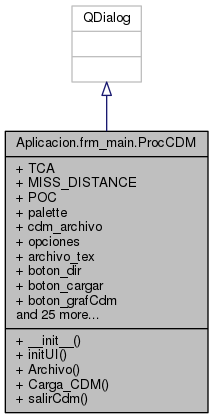
\includegraphics[width=232pt]{class_aplicacion_1_1frm__main_1_1_proc_c_d_m__inherit__graph}
\end{center}
\end{figure}


\-Collaboration diagram for \-Aplicacion.\-frm\-\_\-main.\-Proc\-C\-D\-M\-:\nopagebreak
\begin{figure}[H]
\begin{center}
\leavevmode
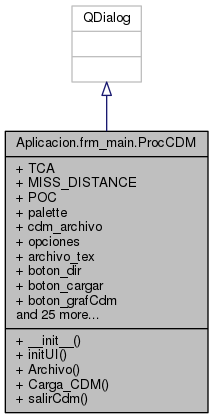
\includegraphics[width=232pt]{class_aplicacion_1_1frm__main_1_1_proc_c_d_m__coll__graph}
\end{center}
\end{figure}
\subsection*{\-Public \-Member \-Functions}
\begin{DoxyCompactItemize}
\item 
def {\bf \-\_\-\-\_\-init\-\_\-\-\_\-}
\item 
def {\bf init\-U\-I}
\item 
def {\bf \-Archivo}
\item 
def {\bf \-Carga\-\_\-\-C\-D\-M}
\item 
def {\bf salir\-Cdm}
\end{DoxyCompactItemize}
\subsection*{\-Public \-Attributes}
\begin{DoxyCompactItemize}
\item 
{\bf \-T\-C\-A}
\item 
{\bf \-M\-I\-S\-S\-\_\-\-D\-I\-S\-T\-A\-N\-C\-E}
\item 
{\bf \-P\-O\-C}
\item 
{\bf palette}
\item 
{\bf cdm\-\_\-archivo}
\item 
{\bf opciones}
\item 
{\bf archivo\-\_\-tex}
\item 
{\bf boton\-\_\-dir}
\item 
{\bf boton\-\_\-cargar}
\item 
{\bf boton\-\_\-graf\-Cdm}
\item 
{\bf boton\-\_\-informe}
\item 
{\bf boton\-\_\-salir\-Cdm}
\item 
{\bf table\-P\-O\-C}
\item 
{\bf cdm\-\_\-xml}
\item 
{\bf cdm\-\_\-nombre}
\item 
{\bf \-C\-D\-M}
\item 
{\bf mision\-\_\-name}
\item 
{\bf norad\-I\-D\-\_\-mision}
\item 
{\bf r\-\_\-sat}
\item 
{\bf v\-\_\-sat}
\item 
{\bf deb\-\_\-name}
\item 
{\bf norad\-I\-D\-\_\-deb}
\item 
{\bf r\-\_\-deb}
\item 
{\bf v\-\_\-deb}
\item 
{\bf dr}
\item 
{\bf ds}
\item 
{\bf dw}
\item 
{\bf rsw\-\_\-vect}
\item 
{\bf cr\-\_\-r}
\item 
{\bf ct\-\_\-r}
\item 
{\bf ct\-\_\-t}
\item 
{\bf cn\-\_\-r}
\item 
{\bf cn\-\_\-t}
\item 
{\bf cn\-\_\-n}
\item 
{\bf cov\-\_\-rtn}
\end{DoxyCompactItemize}


\subsection{\-Detailed \-Description}


\-Definition at line 157 of file frm\-\_\-main.\-py.



\subsection{\-Constructor \& \-Destructor \-Documentation}
\index{\-Aplicacion\-::frm\-\_\-main\-::\-Proc\-C\-D\-M@{\-Aplicacion\-::frm\-\_\-main\-::\-Proc\-C\-D\-M}!\-\_\-\-\_\-init\-\_\-\-\_\-@{\-\_\-\-\_\-init\-\_\-\-\_\-}}
\index{\-\_\-\-\_\-init\-\_\-\-\_\-@{\-\_\-\-\_\-init\-\_\-\-\_\-}!Aplicacion::frm_main::ProcCDM@{\-Aplicacion\-::frm\-\_\-main\-::\-Proc\-C\-D\-M}}
\subsubsection[{\-\_\-\-\_\-init\-\_\-\-\_\-}]{\setlength{\rightskip}{0pt plus 5cm}def {\bf \-Aplicacion.\-frm\-\_\-main.\-Proc\-C\-D\-M.\-\_\-\-\_\-init\-\_\-\-\_\-} (
\begin{DoxyParamCaption}
\item[{}]{self, }
\item[{}]{parent = {\ttfamily \-None}}
\end{DoxyParamCaption}
)}\label{class_aplicacion_1_1frm__main_1_1_proc_c_d_m_a9aff53446934408cdfded450b0968f69}


\-Definition at line 158 of file frm\-\_\-main.\-py.


\begin{DoxyCode}
158 
159     def __init__(self,parent=None):
160         QDialog.__init__(self,parent)
161         
162         self.setWindowModality(Qt.ApplicationModal)
163         self.initUI()
164         
165         # Construccion
166         self.TCA=None
167         self.MISS_DISTANCE=None
168         self.POC=None
169 

\end{DoxyCode}


\subsection{\-Member \-Function \-Documentation}
\index{\-Aplicacion\-::frm\-\_\-main\-::\-Proc\-C\-D\-M@{\-Aplicacion\-::frm\-\_\-main\-::\-Proc\-C\-D\-M}!\-Archivo@{\-Archivo}}
\index{\-Archivo@{\-Archivo}!Aplicacion::frm_main::ProcCDM@{\-Aplicacion\-::frm\-\_\-main\-::\-Proc\-C\-D\-M}}
\subsubsection[{\-Archivo}]{\setlength{\rightskip}{0pt plus 5cm}def {\bf \-Aplicacion.\-frm\-\_\-main.\-Proc\-C\-D\-M.\-Archivo} (
\begin{DoxyParamCaption}
\item[{}]{self}
\end{DoxyParamCaption}
)}\label{class_aplicacion_1_1frm__main_1_1_proc_c_d_m_ad54c9746ccc6b3cae8752f5218382392}


\-Definition at line 237 of file frm\-\_\-main.\-py.


\begin{DoxyCode}
237 
238     def Archivo(self):    
239         self.cdm_xml=QFileDialog.getOpenFileName(self, 'Seleccione el CDM a
       Procesar', "../CDM/archivos/*")
240         self.cdm_nombre=str(self.cdm_xml).split('/')[-1]
241         self.archivo_tex.setText(self.cdm_nombre)
242         
        
\end{DoxyCode}
\index{\-Aplicacion\-::frm\-\_\-main\-::\-Proc\-C\-D\-M@{\-Aplicacion\-::frm\-\_\-main\-::\-Proc\-C\-D\-M}!\-Carga\-\_\-\-C\-D\-M@{\-Carga\-\_\-\-C\-D\-M}}
\index{\-Carga\-\_\-\-C\-D\-M@{\-Carga\-\_\-\-C\-D\-M}!Aplicacion::frm_main::ProcCDM@{\-Aplicacion\-::frm\-\_\-main\-::\-Proc\-C\-D\-M}}
\subsubsection[{\-Carga\-\_\-\-C\-D\-M}]{\setlength{\rightskip}{0pt plus 5cm}def {\bf \-Aplicacion.\-frm\-\_\-main.\-Proc\-C\-D\-M.\-Carga\-\_\-\-C\-D\-M} (
\begin{DoxyParamCaption}
\item[{}]{self}
\end{DoxyParamCaption}
)}\label{class_aplicacion_1_1frm__main_1_1_proc_c_d_m_aed2541f88f0074784be48854f9876cae}


\-Definition at line 243 of file frm\-\_\-main.\-py.


\begin{DoxyCode}
243 
244     def Carga_CDM(self):
245 #        self.cdm_nombre='cdmEnviCosmos08.xml' # seteo el archivo para las
       pruebas
246 #        self.cdm_nombre='cdmTerraPegasus10.xml' # seteo el archivo para las
       pruebas
247         self.CDM=CDM(self.cdm_nombre)
248         self.TCA=self.CDM.TCA
249         self.MISS_DISTANCE=self.CDM.MISS_DISTANCE
250         self.POC=self.CDM.POC
251         self.mision_name=self.CDM.mision_name
252         self.noradID_mision=self.CDM.noradID_mision
253         self.r_sat=self.CDM.r_sat
254         self.v_sat=self.CDM.v_sat
255         self.deb_name=self.CDM.deb_name
256         self.noradID_deb=self.CDM.noradID_deb
257         self.r_deb=self.CDM.r_deb
258         self.v_deb=self.CDM.v_deb
259         # Posiciones Relativas.
260         self.dr=float(self.CDM.dr)/1000.0
261         self.ds=float(self.CDM.ds)/1000.0
262         self.dw=float(self.CDM.dw)/1000.0
263         self.rsw_vect=[self.dr,self.ds,self.dw]
264         # Estadistica 
265         self.cr_r=float(self.CDM.cr_r)*(0.001*0.001)
266         self.ct_r=float(self.CDM.ct_r)*(0.001*0.001)
267         self.ct_t=float(self.CDM.ct_t)*(0.001*0.001)
268         self.cn_r=float(self.CDM.cn_r)*(0.001*0.001)
269         self.cn_t=float(self.CDM.cn_t)*(0.001*0.001)
270         self.cn_n=float(self.CDM.cn_n)*(0.001*0.001) 
271         self.cov_rtn=np.array([[self.cr_r,self.ct_r,self.cn_r],[self.ct_r,self.
      ct_t,self.cn_t],[self.cn_r,self.cn_t,self.cn_n]])     
272         print'**********************'
273         print 'r_sat = ',self.r_sat
274         print 'v_sat = ',self.v_sat
275         print 'r_deb = ',self.r_deb
276         print 'v_deb = ',self.v_deb
277         print self.dr,self.ds,self.dw
278         print '*********************'
279         print self.cr_r
280         print self.ct_r,self.ct_t
281         print self.cn_r,self.cn_t,self.cn_n        
282         #Calculo el angulo entre los vectores velocidad.
283         cos_phi=np.dot(self.v_sat,self.v_deb)/(np.sqrt(np.dot(self.v_sat,self.
      v_sat))*np.sqrt(np.dot(self.v_deb,self.v_deb)))
284         phi=np.arccos(cos_phi) 
285     
286         #Validacion del calculo POC a partir de datos CDM.
287         mu_x,mu_y,sig2_xc,sig2_yc=proyecta_plano_de_encuentro(self.rsw_vect,
      self.cov_rtn,phi)
288         poc, poc_int=calcula_Poc_manual(mu_x, mu_y, sig2_xc, sig2_yc)
289         print '======================'
290         print '------POC-------------'
291         print '======================'
292         print poc, poc_int[0]
293         """
294         Carga de Informacion 
295         """
296         # Cargar la tabla
297         self.tablePOC.setItem(0,0, QTableWidgetItem( self.mision_name))
298         self.tablePOC.setItem(1,0, QTableWidgetItem(self.deb_name))
299         self.tablePOC.setItem(0,1, QTableWidgetItem(self.noradID_mision))
300         self.tablePOC.setItem(1,1, QTableWidgetItem(self.noradID_deb))
301         self.tablePOC.setItem(0,2, QTableWidgetItem(self.TCA))
302         self.tablePOC.setItem(0,3, QTableWidgetItem('TCA arx'))
303         self.tablePOC.setItem(0,4, QTableWidgetItem(self.MISS_DISTANCE))
304         self.tablePOC.setItem(0,5, QTableWidgetItem('M_dist arx'))
305         self.tablePOC.setItem(0,6, QTableWidgetItem(self.POC))
306         self.tablePOC.setItem(0,7, QTableWidgetItem('POC arx'))
307         # formato de tabla
308         header = self.tablePOC.horizontalHeader()
309         header.setResizeMode(0,QHeaderView.Stretch)
310         header.setResizeMode(1,QHeaderView.ResizeToContents)
311         header.setResizeMode(2,QHeaderView.ResizeToContents)
312         header.setResizeMode(3,QHeaderView.ResizeToContents)
313         header.setResizeMode(4,QHeaderView.ResizeToContents)
314         header.setResizeMode(5,QHeaderView.ResizeToContents)
315         header.setResizeMode(6,QHeaderView.ResizeToContents)        
316         header.setResizeMode(7,QHeaderView.ResizeToContents)
317         print 'FIN DE LA CARGA'
        
\end{DoxyCode}
\index{\-Aplicacion\-::frm\-\_\-main\-::\-Proc\-C\-D\-M@{\-Aplicacion\-::frm\-\_\-main\-::\-Proc\-C\-D\-M}!init\-U\-I@{init\-U\-I}}
\index{init\-U\-I@{init\-U\-I}!Aplicacion::frm_main::ProcCDM@{\-Aplicacion\-::frm\-\_\-main\-::\-Proc\-C\-D\-M}}
\subsubsection[{init\-U\-I}]{\setlength{\rightskip}{0pt plus 5cm}def {\bf \-Aplicacion.\-frm\-\_\-main.\-Proc\-C\-D\-M.\-init\-U\-I} (
\begin{DoxyParamCaption}
\item[{}]{self}
\end{DoxyParamCaption}
)}\label{class_aplicacion_1_1frm__main_1_1_proc_c_d_m_a33b199687fcecc96e4d2912d9f0fbf20}


\-Definition at line 170 of file frm\-\_\-main.\-py.


\begin{DoxyCode}
170 
171     def initUI(self):
172         self.palette = QPalette()
173         self.palette.setColor(QPalette.Background,Qt.white)
174         self.setPalette(self.palette)
175         
176         """
177         Etiquetas
178         """
179         self.cdm_archivo = QLabel('Archivo CDM: ')   
180         self.opciones   = QLabel('Opciones')
181         """
182         Campos de Edicion
183         """   
184         self.archivo_tex=QLineEdit('cdmTerraPegasus10.xml') # seteo el archivo
       para las pruebas
185         """
186         Botones
187         """
188         self.boton_dir      = QPushButton('Directorios')
189         self.boton_cargar   = QPushButton('CARGAR')
190         self.boton_grafCdm  = QPushButton('Graficos')
191         self.boton_informe  = QPushButton('Generar Informe')
192         self.boton_salirCdm = QPushButton('SALIR')
193         """
194         OTROS
195         """                
196         moods = [QCheckBox("Posiciones Relativas en RTN"), QCheckBox("
      Procesamiento ARxCODE")] # botones de seleccion
197         self.tablePOC   = QTableWidget() # Tabla con los resultados
198         self.tablePOC.setRowCount(2)
199         self.tablePOC.setColumnCount(8)
200         listaLabels=['Norad Id','Nombre','TCAcdm','TCAarx','MinD cdm','MinD arx
      ','PoC cdm','PoC arx']
201         self.tablePOC.setHorizontalHeaderLabels(listaLabels)
202 
203         
204         grid = QGridLayout()
205         grid.setSpacing(5)
206         
207         grid.addWidget(self.cdm_archivo,2,1)
208         grid.addWidget(self.archivo_tex,2,2)
209         grid.addWidget(self.boton_dir,2,3)
210         grid.addWidget( self.opciones,3,1)
211         grid.addWidget(moods[0],4,2)     
212         grid.addWidget(moods[1],5,2)
213         grid.addWidget(self.boton_cargar,6,3)
214 #         grid.addWidget(self.boton_grafCdm,4,2)
215 #         grid.addWidget(self.boton_informe,5,2)
216         grid.addWidget(self.boton_salirCdm,18,2)
217         grid.addWidget(self.tablePOC,8,1,3,7)
218 
219         
220         self.setLayout(grid)
221         self.setWindowTitle('Procesamiento de CDM')    
222         self.show()
223         
224         """
225         Acciones
226         """
227         self.boton_dir.clicked.connect(self.Archivo)
228         self.boton_cargar.clicked.connect(self.Carga_CDM)
229         self.boton_salirCdm.clicked.connect(self.salirCdm)
230         
231 
232 #        
       TCAc,mod_dif,poc=evaluaEncuentro(self.TCA,self.sat_idc,self.deb_idc,Cd,Cm)
233 #         TCAstr=datetime.strftime(TCAc,'%Y-%m-%d %H:%M:%S.%f')
234 #         mod_dif=int(mod_dif*1000.0)
235 #         # set data self.TCA, self.MISS_DISTANCE,self.POC
236 

\end{DoxyCode}


\-Here is the caller graph for this function\-:\nopagebreak
\begin{figure}[H]
\begin{center}
\leavevmode
\includegraphics[width=350pt]{class_aplicacion_1_1frm__main_1_1_proc_c_d_m_a33b199687fcecc96e4d2912d9f0fbf20_icgraph}
\end{center}
\end{figure}


\index{\-Aplicacion\-::frm\-\_\-main\-::\-Proc\-C\-D\-M@{\-Aplicacion\-::frm\-\_\-main\-::\-Proc\-C\-D\-M}!salir\-Cdm@{salir\-Cdm}}
\index{salir\-Cdm@{salir\-Cdm}!Aplicacion::frm_main::ProcCDM@{\-Aplicacion\-::frm\-\_\-main\-::\-Proc\-C\-D\-M}}
\subsubsection[{salir\-Cdm}]{\setlength{\rightskip}{0pt plus 5cm}def {\bf \-Aplicacion.\-frm\-\_\-main.\-Proc\-C\-D\-M.\-salir\-Cdm} (
\begin{DoxyParamCaption}
\item[{}]{self}
\end{DoxyParamCaption}
)}\label{class_aplicacion_1_1frm__main_1_1_proc_c_d_m_a6078f86c360fc473378c37871bc276c1}


\-Definition at line 318 of file frm\-\_\-main.\-py.


\begin{DoxyCode}
318 
319     def salirCdm(self):
320         self.accept()
321 
        
\end{DoxyCode}


\subsection{\-Member \-Data \-Documentation}
\index{\-Aplicacion\-::frm\-\_\-main\-::\-Proc\-C\-D\-M@{\-Aplicacion\-::frm\-\_\-main\-::\-Proc\-C\-D\-M}!archivo\-\_\-tex@{archivo\-\_\-tex}}
\index{archivo\-\_\-tex@{archivo\-\_\-tex}!Aplicacion::frm_main::ProcCDM@{\-Aplicacion\-::frm\-\_\-main\-::\-Proc\-C\-D\-M}}
\subsubsection[{archivo\-\_\-tex}]{\setlength{\rightskip}{0pt plus 5cm}{\bf \-Aplicacion\-::frm\-\_\-main.\-Proc\-C\-D\-M\-::archivo\-\_\-tex}}\label{class_aplicacion_1_1frm__main_1_1_proc_c_d_m_ab7b1fc2d236fed165a4ecffae0826885}


\-Definition at line 174 of file frm\-\_\-main.\-py.

\index{\-Aplicacion\-::frm\-\_\-main\-::\-Proc\-C\-D\-M@{\-Aplicacion\-::frm\-\_\-main\-::\-Proc\-C\-D\-M}!boton\-\_\-cargar@{boton\-\_\-cargar}}
\index{boton\-\_\-cargar@{boton\-\_\-cargar}!Aplicacion::frm_main::ProcCDM@{\-Aplicacion\-::frm\-\_\-main\-::\-Proc\-C\-D\-M}}
\subsubsection[{boton\-\_\-cargar}]{\setlength{\rightskip}{0pt plus 5cm}{\bf \-Aplicacion\-::frm\-\_\-main.\-Proc\-C\-D\-M\-::boton\-\_\-cargar}}\label{class_aplicacion_1_1frm__main_1_1_proc_c_d_m_a5711d6b7029f242b87d527c1bb6842bb}


\-Definition at line 176 of file frm\-\_\-main.\-py.

\index{\-Aplicacion\-::frm\-\_\-main\-::\-Proc\-C\-D\-M@{\-Aplicacion\-::frm\-\_\-main\-::\-Proc\-C\-D\-M}!boton\-\_\-dir@{boton\-\_\-dir}}
\index{boton\-\_\-dir@{boton\-\_\-dir}!Aplicacion::frm_main::ProcCDM@{\-Aplicacion\-::frm\-\_\-main\-::\-Proc\-C\-D\-M}}
\subsubsection[{boton\-\_\-dir}]{\setlength{\rightskip}{0pt plus 5cm}{\bf \-Aplicacion\-::frm\-\_\-main.\-Proc\-C\-D\-M\-::boton\-\_\-dir}}\label{class_aplicacion_1_1frm__main_1_1_proc_c_d_m_a05c4f93bc30ea030b37a7a881725d512}


\-Definition at line 176 of file frm\-\_\-main.\-py.

\index{\-Aplicacion\-::frm\-\_\-main\-::\-Proc\-C\-D\-M@{\-Aplicacion\-::frm\-\_\-main\-::\-Proc\-C\-D\-M}!boton\-\_\-graf\-Cdm@{boton\-\_\-graf\-Cdm}}
\index{boton\-\_\-graf\-Cdm@{boton\-\_\-graf\-Cdm}!Aplicacion::frm_main::ProcCDM@{\-Aplicacion\-::frm\-\_\-main\-::\-Proc\-C\-D\-M}}
\subsubsection[{boton\-\_\-graf\-Cdm}]{\setlength{\rightskip}{0pt plus 5cm}{\bf \-Aplicacion\-::frm\-\_\-main.\-Proc\-C\-D\-M\-::boton\-\_\-graf\-Cdm}}\label{class_aplicacion_1_1frm__main_1_1_proc_c_d_m_ac86bc089a875acc78843824ca78d286c}


\-Definition at line 176 of file frm\-\_\-main.\-py.

\index{\-Aplicacion\-::frm\-\_\-main\-::\-Proc\-C\-D\-M@{\-Aplicacion\-::frm\-\_\-main\-::\-Proc\-C\-D\-M}!boton\-\_\-informe@{boton\-\_\-informe}}
\index{boton\-\_\-informe@{boton\-\_\-informe}!Aplicacion::frm_main::ProcCDM@{\-Aplicacion\-::frm\-\_\-main\-::\-Proc\-C\-D\-M}}
\subsubsection[{boton\-\_\-informe}]{\setlength{\rightskip}{0pt plus 5cm}{\bf \-Aplicacion\-::frm\-\_\-main.\-Proc\-C\-D\-M\-::boton\-\_\-informe}}\label{class_aplicacion_1_1frm__main_1_1_proc_c_d_m_acb483334d88f558ace6d2174521dd982}


\-Definition at line 176 of file frm\-\_\-main.\-py.

\index{\-Aplicacion\-::frm\-\_\-main\-::\-Proc\-C\-D\-M@{\-Aplicacion\-::frm\-\_\-main\-::\-Proc\-C\-D\-M}!boton\-\_\-salir\-Cdm@{boton\-\_\-salir\-Cdm}}
\index{boton\-\_\-salir\-Cdm@{boton\-\_\-salir\-Cdm}!Aplicacion::frm_main::ProcCDM@{\-Aplicacion\-::frm\-\_\-main\-::\-Proc\-C\-D\-M}}
\subsubsection[{boton\-\_\-salir\-Cdm}]{\setlength{\rightskip}{0pt plus 5cm}{\bf \-Aplicacion\-::frm\-\_\-main.\-Proc\-C\-D\-M\-::boton\-\_\-salir\-Cdm}}\label{class_aplicacion_1_1frm__main_1_1_proc_c_d_m_a18aa5750b77a458dbd44a6fe96688186}


\-Definition at line 176 of file frm\-\_\-main.\-py.

\index{\-Aplicacion\-::frm\-\_\-main\-::\-Proc\-C\-D\-M@{\-Aplicacion\-::frm\-\_\-main\-::\-Proc\-C\-D\-M}!\-C\-D\-M@{\-C\-D\-M}}
\index{\-C\-D\-M@{\-C\-D\-M}!Aplicacion::frm_main::ProcCDM@{\-Aplicacion\-::frm\-\_\-main\-::\-Proc\-C\-D\-M}}
\subsubsection[{\-C\-D\-M}]{\setlength{\rightskip}{0pt plus 5cm}{\bf \-Aplicacion\-::frm\-\_\-main.\-Proc\-C\-D\-M\-::\-C\-D\-M}}\label{class_aplicacion_1_1frm__main_1_1_proc_c_d_m_af608a21996b27b7cd0bb10563fc9e96b}


\-Definition at line 245 of file frm\-\_\-main.\-py.

\index{\-Aplicacion\-::frm\-\_\-main\-::\-Proc\-C\-D\-M@{\-Aplicacion\-::frm\-\_\-main\-::\-Proc\-C\-D\-M}!cdm\-\_\-archivo@{cdm\-\_\-archivo}}
\index{cdm\-\_\-archivo@{cdm\-\_\-archivo}!Aplicacion::frm_main::ProcCDM@{\-Aplicacion\-::frm\-\_\-main\-::\-Proc\-C\-D\-M}}
\subsubsection[{cdm\-\_\-archivo}]{\setlength{\rightskip}{0pt plus 5cm}{\bf \-Aplicacion\-::frm\-\_\-main.\-Proc\-C\-D\-M\-::cdm\-\_\-archivo}}\label{class_aplicacion_1_1frm__main_1_1_proc_c_d_m_a54f6f5bd86de7195c64800f4b4d5f550}


\-Definition at line 172 of file frm\-\_\-main.\-py.

\index{\-Aplicacion\-::frm\-\_\-main\-::\-Proc\-C\-D\-M@{\-Aplicacion\-::frm\-\_\-main\-::\-Proc\-C\-D\-M}!cdm\-\_\-nombre@{cdm\-\_\-nombre}}
\index{cdm\-\_\-nombre@{cdm\-\_\-nombre}!Aplicacion::frm_main::ProcCDM@{\-Aplicacion\-::frm\-\_\-main\-::\-Proc\-C\-D\-M}}
\subsubsection[{cdm\-\_\-nombre}]{\setlength{\rightskip}{0pt plus 5cm}{\bf \-Aplicacion\-::frm\-\_\-main.\-Proc\-C\-D\-M\-::cdm\-\_\-nombre}}\label{class_aplicacion_1_1frm__main_1_1_proc_c_d_m_ae9b065153b32988b2b7b3f75bd1dee55}


\-Definition at line 237 of file frm\-\_\-main.\-py.

\index{\-Aplicacion\-::frm\-\_\-main\-::\-Proc\-C\-D\-M@{\-Aplicacion\-::frm\-\_\-main\-::\-Proc\-C\-D\-M}!cdm\-\_\-xml@{cdm\-\_\-xml}}
\index{cdm\-\_\-xml@{cdm\-\_\-xml}!Aplicacion::frm_main::ProcCDM@{\-Aplicacion\-::frm\-\_\-main\-::\-Proc\-C\-D\-M}}
\subsubsection[{cdm\-\_\-xml}]{\setlength{\rightskip}{0pt plus 5cm}{\bf \-Aplicacion\-::frm\-\_\-main.\-Proc\-C\-D\-M\-::cdm\-\_\-xml}}\label{class_aplicacion_1_1frm__main_1_1_proc_c_d_m_a92d0f7594213d5cf23a6a8a3b0dcf568}


\-Definition at line 237 of file frm\-\_\-main.\-py.

\index{\-Aplicacion\-::frm\-\_\-main\-::\-Proc\-C\-D\-M@{\-Aplicacion\-::frm\-\_\-main\-::\-Proc\-C\-D\-M}!cn\-\_\-n@{cn\-\_\-n}}
\index{cn\-\_\-n@{cn\-\_\-n}!Aplicacion::frm_main::ProcCDM@{\-Aplicacion\-::frm\-\_\-main\-::\-Proc\-C\-D\-M}}
\subsubsection[{cn\-\_\-n}]{\setlength{\rightskip}{0pt plus 5cm}{\bf \-Aplicacion\-::frm\-\_\-main.\-Proc\-C\-D\-M\-::cn\-\_\-n}}\label{class_aplicacion_1_1frm__main_1_1_proc_c_d_m_a7a690279821ce424c8974c87eea9aca1}


\-Definition at line 245 of file frm\-\_\-main.\-py.

\index{\-Aplicacion\-::frm\-\_\-main\-::\-Proc\-C\-D\-M@{\-Aplicacion\-::frm\-\_\-main\-::\-Proc\-C\-D\-M}!cn\-\_\-r@{cn\-\_\-r}}
\index{cn\-\_\-r@{cn\-\_\-r}!Aplicacion::frm_main::ProcCDM@{\-Aplicacion\-::frm\-\_\-main\-::\-Proc\-C\-D\-M}}
\subsubsection[{cn\-\_\-r}]{\setlength{\rightskip}{0pt plus 5cm}{\bf \-Aplicacion\-::frm\-\_\-main.\-Proc\-C\-D\-M\-::cn\-\_\-r}}\label{class_aplicacion_1_1frm__main_1_1_proc_c_d_m_a315411041da65429f698d23b9ab7d395}


\-Definition at line 245 of file frm\-\_\-main.\-py.

\index{\-Aplicacion\-::frm\-\_\-main\-::\-Proc\-C\-D\-M@{\-Aplicacion\-::frm\-\_\-main\-::\-Proc\-C\-D\-M}!cn\-\_\-t@{cn\-\_\-t}}
\index{cn\-\_\-t@{cn\-\_\-t}!Aplicacion::frm_main::ProcCDM@{\-Aplicacion\-::frm\-\_\-main\-::\-Proc\-C\-D\-M}}
\subsubsection[{cn\-\_\-t}]{\setlength{\rightskip}{0pt plus 5cm}{\bf \-Aplicacion\-::frm\-\_\-main.\-Proc\-C\-D\-M\-::cn\-\_\-t}}\label{class_aplicacion_1_1frm__main_1_1_proc_c_d_m_a254519a3937bdd9f5e8d0e4436463be1}


\-Definition at line 245 of file frm\-\_\-main.\-py.

\index{\-Aplicacion\-::frm\-\_\-main\-::\-Proc\-C\-D\-M@{\-Aplicacion\-::frm\-\_\-main\-::\-Proc\-C\-D\-M}!cov\-\_\-rtn@{cov\-\_\-rtn}}
\index{cov\-\_\-rtn@{cov\-\_\-rtn}!Aplicacion::frm_main::ProcCDM@{\-Aplicacion\-::frm\-\_\-main\-::\-Proc\-C\-D\-M}}
\subsubsection[{cov\-\_\-rtn}]{\setlength{\rightskip}{0pt plus 5cm}{\bf \-Aplicacion\-::frm\-\_\-main.\-Proc\-C\-D\-M\-::cov\-\_\-rtn}}\label{class_aplicacion_1_1frm__main_1_1_proc_c_d_m_ae77c3984c00ccdd317043b9432f70724}


\-Definition at line 245 of file frm\-\_\-main.\-py.

\index{\-Aplicacion\-::frm\-\_\-main\-::\-Proc\-C\-D\-M@{\-Aplicacion\-::frm\-\_\-main\-::\-Proc\-C\-D\-M}!cr\-\_\-r@{cr\-\_\-r}}
\index{cr\-\_\-r@{cr\-\_\-r}!Aplicacion::frm_main::ProcCDM@{\-Aplicacion\-::frm\-\_\-main\-::\-Proc\-C\-D\-M}}
\subsubsection[{cr\-\_\-r}]{\setlength{\rightskip}{0pt plus 5cm}{\bf \-Aplicacion\-::frm\-\_\-main.\-Proc\-C\-D\-M\-::cr\-\_\-r}}\label{class_aplicacion_1_1frm__main_1_1_proc_c_d_m_a6a445fa10747b5ef7f5287ed1d9543ab}


\-Definition at line 245 of file frm\-\_\-main.\-py.

\index{\-Aplicacion\-::frm\-\_\-main\-::\-Proc\-C\-D\-M@{\-Aplicacion\-::frm\-\_\-main\-::\-Proc\-C\-D\-M}!ct\-\_\-r@{ct\-\_\-r}}
\index{ct\-\_\-r@{ct\-\_\-r}!Aplicacion::frm_main::ProcCDM@{\-Aplicacion\-::frm\-\_\-main\-::\-Proc\-C\-D\-M}}
\subsubsection[{ct\-\_\-r}]{\setlength{\rightskip}{0pt plus 5cm}{\bf \-Aplicacion\-::frm\-\_\-main.\-Proc\-C\-D\-M\-::ct\-\_\-r}}\label{class_aplicacion_1_1frm__main_1_1_proc_c_d_m_adff3c04b7f06dfe44c4353cb903272df}


\-Definition at line 245 of file frm\-\_\-main.\-py.

\index{\-Aplicacion\-::frm\-\_\-main\-::\-Proc\-C\-D\-M@{\-Aplicacion\-::frm\-\_\-main\-::\-Proc\-C\-D\-M}!ct\-\_\-t@{ct\-\_\-t}}
\index{ct\-\_\-t@{ct\-\_\-t}!Aplicacion::frm_main::ProcCDM@{\-Aplicacion\-::frm\-\_\-main\-::\-Proc\-C\-D\-M}}
\subsubsection[{ct\-\_\-t}]{\setlength{\rightskip}{0pt plus 5cm}{\bf \-Aplicacion\-::frm\-\_\-main.\-Proc\-C\-D\-M\-::ct\-\_\-t}}\label{class_aplicacion_1_1frm__main_1_1_proc_c_d_m_af01e616ddf626901bd7cbdf071f421b7}


\-Definition at line 245 of file frm\-\_\-main.\-py.

\index{\-Aplicacion\-::frm\-\_\-main\-::\-Proc\-C\-D\-M@{\-Aplicacion\-::frm\-\_\-main\-::\-Proc\-C\-D\-M}!deb\-\_\-name@{deb\-\_\-name}}
\index{deb\-\_\-name@{deb\-\_\-name}!Aplicacion::frm_main::ProcCDM@{\-Aplicacion\-::frm\-\_\-main\-::\-Proc\-C\-D\-M}}
\subsubsection[{deb\-\_\-name}]{\setlength{\rightskip}{0pt plus 5cm}{\bf \-Aplicacion\-::frm\-\_\-main.\-Proc\-C\-D\-M\-::deb\-\_\-name}}\label{class_aplicacion_1_1frm__main_1_1_proc_c_d_m_a84a06b8222490907b4447f3fb86e7d1c}


\-Definition at line 245 of file frm\-\_\-main.\-py.

\index{\-Aplicacion\-::frm\-\_\-main\-::\-Proc\-C\-D\-M@{\-Aplicacion\-::frm\-\_\-main\-::\-Proc\-C\-D\-M}!dr@{dr}}
\index{dr@{dr}!Aplicacion::frm_main::ProcCDM@{\-Aplicacion\-::frm\-\_\-main\-::\-Proc\-C\-D\-M}}
\subsubsection[{dr}]{\setlength{\rightskip}{0pt plus 5cm}{\bf \-Aplicacion\-::frm\-\_\-main.\-Proc\-C\-D\-M\-::dr}}\label{class_aplicacion_1_1frm__main_1_1_proc_c_d_m_a7ebcb1ad8d0289c49c02492540823a50}


\-Definition at line 245 of file frm\-\_\-main.\-py.

\index{\-Aplicacion\-::frm\-\_\-main\-::\-Proc\-C\-D\-M@{\-Aplicacion\-::frm\-\_\-main\-::\-Proc\-C\-D\-M}!ds@{ds}}
\index{ds@{ds}!Aplicacion::frm_main::ProcCDM@{\-Aplicacion\-::frm\-\_\-main\-::\-Proc\-C\-D\-M}}
\subsubsection[{ds}]{\setlength{\rightskip}{0pt plus 5cm}{\bf \-Aplicacion\-::frm\-\_\-main.\-Proc\-C\-D\-M\-::ds}}\label{class_aplicacion_1_1frm__main_1_1_proc_c_d_m_a72e1a29ff114577ff2b01b7eae8440ab}


\-Definition at line 245 of file frm\-\_\-main.\-py.

\index{\-Aplicacion\-::frm\-\_\-main\-::\-Proc\-C\-D\-M@{\-Aplicacion\-::frm\-\_\-main\-::\-Proc\-C\-D\-M}!dw@{dw}}
\index{dw@{dw}!Aplicacion::frm_main::ProcCDM@{\-Aplicacion\-::frm\-\_\-main\-::\-Proc\-C\-D\-M}}
\subsubsection[{dw}]{\setlength{\rightskip}{0pt plus 5cm}{\bf \-Aplicacion\-::frm\-\_\-main.\-Proc\-C\-D\-M\-::dw}}\label{class_aplicacion_1_1frm__main_1_1_proc_c_d_m_ab8e621e7e023196ab30910df106922fe}


\-Definition at line 245 of file frm\-\_\-main.\-py.

\index{\-Aplicacion\-::frm\-\_\-main\-::\-Proc\-C\-D\-M@{\-Aplicacion\-::frm\-\_\-main\-::\-Proc\-C\-D\-M}!mision\-\_\-name@{mision\-\_\-name}}
\index{mision\-\_\-name@{mision\-\_\-name}!Aplicacion::frm_main::ProcCDM@{\-Aplicacion\-::frm\-\_\-main\-::\-Proc\-C\-D\-M}}
\subsubsection[{mision\-\_\-name}]{\setlength{\rightskip}{0pt plus 5cm}{\bf \-Aplicacion\-::frm\-\_\-main.\-Proc\-C\-D\-M\-::mision\-\_\-name}}\label{class_aplicacion_1_1frm__main_1_1_proc_c_d_m_aa065da97b64d80f7d800f2638a15e2e2}


\-Definition at line 245 of file frm\-\_\-main.\-py.

\index{\-Aplicacion\-::frm\-\_\-main\-::\-Proc\-C\-D\-M@{\-Aplicacion\-::frm\-\_\-main\-::\-Proc\-C\-D\-M}!\-M\-I\-S\-S\-\_\-\-D\-I\-S\-T\-A\-N\-C\-E@{\-M\-I\-S\-S\-\_\-\-D\-I\-S\-T\-A\-N\-C\-E}}
\index{\-M\-I\-S\-S\-\_\-\-D\-I\-S\-T\-A\-N\-C\-E@{\-M\-I\-S\-S\-\_\-\-D\-I\-S\-T\-A\-N\-C\-E}!Aplicacion::frm_main::ProcCDM@{\-Aplicacion\-::frm\-\_\-main\-::\-Proc\-C\-D\-M}}
\subsubsection[{\-M\-I\-S\-S\-\_\-\-D\-I\-S\-T\-A\-N\-C\-E}]{\setlength{\rightskip}{0pt plus 5cm}{\bf \-Aplicacion\-::frm\-\_\-main.\-Proc\-C\-D\-M\-::\-M\-I\-S\-S\-\_\-\-D\-I\-S\-T\-A\-N\-C\-E}}\label{class_aplicacion_1_1frm__main_1_1_proc_c_d_m_a512ea2358325a44d64f33dfade076dcc}


\-Definition at line 158 of file frm\-\_\-main.\-py.

\index{\-Aplicacion\-::frm\-\_\-main\-::\-Proc\-C\-D\-M@{\-Aplicacion\-::frm\-\_\-main\-::\-Proc\-C\-D\-M}!norad\-I\-D\-\_\-deb@{norad\-I\-D\-\_\-deb}}
\index{norad\-I\-D\-\_\-deb@{norad\-I\-D\-\_\-deb}!Aplicacion::frm_main::ProcCDM@{\-Aplicacion\-::frm\-\_\-main\-::\-Proc\-C\-D\-M}}
\subsubsection[{norad\-I\-D\-\_\-deb}]{\setlength{\rightskip}{0pt plus 5cm}{\bf \-Aplicacion\-::frm\-\_\-main.\-Proc\-C\-D\-M\-::norad\-I\-D\-\_\-deb}}\label{class_aplicacion_1_1frm__main_1_1_proc_c_d_m_a9a4fa3d1689053b3943bdfa242a26eda}


\-Definition at line 245 of file frm\-\_\-main.\-py.

\index{\-Aplicacion\-::frm\-\_\-main\-::\-Proc\-C\-D\-M@{\-Aplicacion\-::frm\-\_\-main\-::\-Proc\-C\-D\-M}!norad\-I\-D\-\_\-mision@{norad\-I\-D\-\_\-mision}}
\index{norad\-I\-D\-\_\-mision@{norad\-I\-D\-\_\-mision}!Aplicacion::frm_main::ProcCDM@{\-Aplicacion\-::frm\-\_\-main\-::\-Proc\-C\-D\-M}}
\subsubsection[{norad\-I\-D\-\_\-mision}]{\setlength{\rightskip}{0pt plus 5cm}{\bf \-Aplicacion\-::frm\-\_\-main.\-Proc\-C\-D\-M\-::norad\-I\-D\-\_\-mision}}\label{class_aplicacion_1_1frm__main_1_1_proc_c_d_m_a01dfddf25e9e718e7e05a1c6d4e9e7f7}


\-Definition at line 245 of file frm\-\_\-main.\-py.

\index{\-Aplicacion\-::frm\-\_\-main\-::\-Proc\-C\-D\-M@{\-Aplicacion\-::frm\-\_\-main\-::\-Proc\-C\-D\-M}!opciones@{opciones}}
\index{opciones@{opciones}!Aplicacion::frm_main::ProcCDM@{\-Aplicacion\-::frm\-\_\-main\-::\-Proc\-C\-D\-M}}
\subsubsection[{opciones}]{\setlength{\rightskip}{0pt plus 5cm}{\bf \-Aplicacion\-::frm\-\_\-main.\-Proc\-C\-D\-M\-::opciones}}\label{class_aplicacion_1_1frm__main_1_1_proc_c_d_m_a65331fe7e9064330ebd0be10822f0571}


\-Definition at line 172 of file frm\-\_\-main.\-py.

\index{\-Aplicacion\-::frm\-\_\-main\-::\-Proc\-C\-D\-M@{\-Aplicacion\-::frm\-\_\-main\-::\-Proc\-C\-D\-M}!palette@{palette}}
\index{palette@{palette}!Aplicacion::frm_main::ProcCDM@{\-Aplicacion\-::frm\-\_\-main\-::\-Proc\-C\-D\-M}}
\subsubsection[{palette}]{\setlength{\rightskip}{0pt plus 5cm}{\bf \-Aplicacion\-::frm\-\_\-main.\-Proc\-C\-D\-M\-::palette}}\label{class_aplicacion_1_1frm__main_1_1_proc_c_d_m_aada760c2d77c59bc0054e7a38bc571ac}


\-Definition at line 170 of file frm\-\_\-main.\-py.

\index{\-Aplicacion\-::frm\-\_\-main\-::\-Proc\-C\-D\-M@{\-Aplicacion\-::frm\-\_\-main\-::\-Proc\-C\-D\-M}!\-P\-O\-C@{\-P\-O\-C}}
\index{\-P\-O\-C@{\-P\-O\-C}!Aplicacion::frm_main::ProcCDM@{\-Aplicacion\-::frm\-\_\-main\-::\-Proc\-C\-D\-M}}
\subsubsection[{\-P\-O\-C}]{\setlength{\rightskip}{0pt plus 5cm}{\bf \-Aplicacion\-::frm\-\_\-main.\-Proc\-C\-D\-M\-::\-P\-O\-C}}\label{class_aplicacion_1_1frm__main_1_1_proc_c_d_m_aac37760ecdaf03cabf2e9ec4e2b21d97}


\-Definition at line 158 of file frm\-\_\-main.\-py.

\index{\-Aplicacion\-::frm\-\_\-main\-::\-Proc\-C\-D\-M@{\-Aplicacion\-::frm\-\_\-main\-::\-Proc\-C\-D\-M}!r\-\_\-deb@{r\-\_\-deb}}
\index{r\-\_\-deb@{r\-\_\-deb}!Aplicacion::frm_main::ProcCDM@{\-Aplicacion\-::frm\-\_\-main\-::\-Proc\-C\-D\-M}}
\subsubsection[{r\-\_\-deb}]{\setlength{\rightskip}{0pt plus 5cm}{\bf \-Aplicacion\-::frm\-\_\-main.\-Proc\-C\-D\-M\-::r\-\_\-deb}}\label{class_aplicacion_1_1frm__main_1_1_proc_c_d_m_a10c2a89ce69afb1803e02bfe61882e22}


\-Definition at line 245 of file frm\-\_\-main.\-py.

\index{\-Aplicacion\-::frm\-\_\-main\-::\-Proc\-C\-D\-M@{\-Aplicacion\-::frm\-\_\-main\-::\-Proc\-C\-D\-M}!r\-\_\-sat@{r\-\_\-sat}}
\index{r\-\_\-sat@{r\-\_\-sat}!Aplicacion::frm_main::ProcCDM@{\-Aplicacion\-::frm\-\_\-main\-::\-Proc\-C\-D\-M}}
\subsubsection[{r\-\_\-sat}]{\setlength{\rightskip}{0pt plus 5cm}{\bf \-Aplicacion\-::frm\-\_\-main.\-Proc\-C\-D\-M\-::r\-\_\-sat}}\label{class_aplicacion_1_1frm__main_1_1_proc_c_d_m_abe62806df6944a0b1877de83636f1c4f}


\-Definition at line 245 of file frm\-\_\-main.\-py.

\index{\-Aplicacion\-::frm\-\_\-main\-::\-Proc\-C\-D\-M@{\-Aplicacion\-::frm\-\_\-main\-::\-Proc\-C\-D\-M}!rsw\-\_\-vect@{rsw\-\_\-vect}}
\index{rsw\-\_\-vect@{rsw\-\_\-vect}!Aplicacion::frm_main::ProcCDM@{\-Aplicacion\-::frm\-\_\-main\-::\-Proc\-C\-D\-M}}
\subsubsection[{rsw\-\_\-vect}]{\setlength{\rightskip}{0pt plus 5cm}{\bf \-Aplicacion\-::frm\-\_\-main.\-Proc\-C\-D\-M\-::rsw\-\_\-vect}}\label{class_aplicacion_1_1frm__main_1_1_proc_c_d_m_ac5bfa96912f033d09ebf7e6a1adc8dab}


\-Definition at line 245 of file frm\-\_\-main.\-py.

\index{\-Aplicacion\-::frm\-\_\-main\-::\-Proc\-C\-D\-M@{\-Aplicacion\-::frm\-\_\-main\-::\-Proc\-C\-D\-M}!table\-P\-O\-C@{table\-P\-O\-C}}
\index{table\-P\-O\-C@{table\-P\-O\-C}!Aplicacion::frm_main::ProcCDM@{\-Aplicacion\-::frm\-\_\-main\-::\-Proc\-C\-D\-M}}
\subsubsection[{table\-P\-O\-C}]{\setlength{\rightskip}{0pt plus 5cm}{\bf \-Aplicacion\-::frm\-\_\-main.\-Proc\-C\-D\-M\-::table\-P\-O\-C}}\label{class_aplicacion_1_1frm__main_1_1_proc_c_d_m_a00e6ed32fb0248050fb7f5882aa44f26}


\-Definition at line 178 of file frm\-\_\-main.\-py.

\index{\-Aplicacion\-::frm\-\_\-main\-::\-Proc\-C\-D\-M@{\-Aplicacion\-::frm\-\_\-main\-::\-Proc\-C\-D\-M}!\-T\-C\-A@{\-T\-C\-A}}
\index{\-T\-C\-A@{\-T\-C\-A}!Aplicacion::frm_main::ProcCDM@{\-Aplicacion\-::frm\-\_\-main\-::\-Proc\-C\-D\-M}}
\subsubsection[{\-T\-C\-A}]{\setlength{\rightskip}{0pt plus 5cm}{\bf \-Aplicacion\-::frm\-\_\-main.\-Proc\-C\-D\-M\-::\-T\-C\-A}}\label{class_aplicacion_1_1frm__main_1_1_proc_c_d_m_abe1e1e647122ef84eb86b2707b3bbc79}


\-Definition at line 158 of file frm\-\_\-main.\-py.

\index{\-Aplicacion\-::frm\-\_\-main\-::\-Proc\-C\-D\-M@{\-Aplicacion\-::frm\-\_\-main\-::\-Proc\-C\-D\-M}!v\-\_\-deb@{v\-\_\-deb}}
\index{v\-\_\-deb@{v\-\_\-deb}!Aplicacion::frm_main::ProcCDM@{\-Aplicacion\-::frm\-\_\-main\-::\-Proc\-C\-D\-M}}
\subsubsection[{v\-\_\-deb}]{\setlength{\rightskip}{0pt plus 5cm}{\bf \-Aplicacion\-::frm\-\_\-main.\-Proc\-C\-D\-M\-::v\-\_\-deb}}\label{class_aplicacion_1_1frm__main_1_1_proc_c_d_m_ad67ceb349235b172f12ab6c51fffa51c}


\-Definition at line 245 of file frm\-\_\-main.\-py.

\index{\-Aplicacion\-::frm\-\_\-main\-::\-Proc\-C\-D\-M@{\-Aplicacion\-::frm\-\_\-main\-::\-Proc\-C\-D\-M}!v\-\_\-sat@{v\-\_\-sat}}
\index{v\-\_\-sat@{v\-\_\-sat}!Aplicacion::frm_main::ProcCDM@{\-Aplicacion\-::frm\-\_\-main\-::\-Proc\-C\-D\-M}}
\subsubsection[{v\-\_\-sat}]{\setlength{\rightskip}{0pt plus 5cm}{\bf \-Aplicacion\-::frm\-\_\-main.\-Proc\-C\-D\-M\-::v\-\_\-sat}}\label{class_aplicacion_1_1frm__main_1_1_proc_c_d_m_ab9af407588f41665563bfc941b3063b9}


\-Definition at line 245 of file frm\-\_\-main.\-py.



\-The documentation for this class was generated from the following file\-:\begin{DoxyCompactItemize}
\item 
\-Aplicacion/{\bf frm\-\_\-main.\-py}\end{DoxyCompactItemize}

\section{\-Aplicacion\-C\-O\-D\-S.\-C\-O\-D\-Sinterface.\-Proc\-C\-O\-D\-S \-Class \-Reference}
\label{class_aplicacion_c_o_d_s_1_1_c_o_d_sinterface_1_1_proc_c_o_d_s}\index{\-Aplicacion\-C\-O\-D\-S.\-C\-O\-D\-Sinterface.\-Proc\-C\-O\-D\-S@{\-Aplicacion\-C\-O\-D\-S.\-C\-O\-D\-Sinterface.\-Proc\-C\-O\-D\-S}}


\-Inheritance diagram for \-Aplicacion\-C\-O\-D\-S.\-C\-O\-D\-Sinterface.\-Proc\-C\-O\-D\-S\-:\nopagebreak
\begin{figure}[H]
\begin{center}
\leavevmode
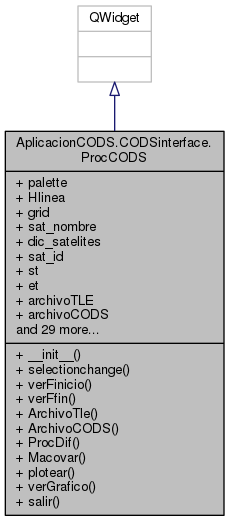
\includegraphics[width=292pt]{class_aplicacion_c_o_d_s_1_1_c_o_d_sinterface_1_1_proc_c_o_d_s__inherit__graph}
\end{center}
\end{figure}


\-Collaboration diagram for \-Aplicacion\-C\-O\-D\-S.\-C\-O\-D\-Sinterface.\-Proc\-C\-O\-D\-S\-:\nopagebreak
\begin{figure}[H]
\begin{center}
\leavevmode
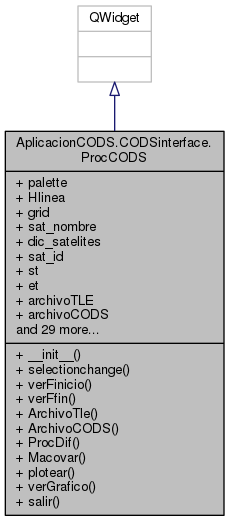
\includegraphics[width=292pt]{class_aplicacion_c_o_d_s_1_1_c_o_d_sinterface_1_1_proc_c_o_d_s__coll__graph}
\end{center}
\end{figure}
\subsection*{\-Public \-Member \-Functions}
\begin{DoxyCompactItemize}
\item 
def {\bf \-\_\-\-\_\-init\-\_\-\-\_\-}
\item 
def {\bf selectionchange}
\item 
def {\bf ver\-Finicio}
\item 
def {\bf ver\-Ffin}
\item 
def {\bf \-Archivo\-Tle}
\item 
def {\bf \-Archivo\-C\-O\-D\-S}
\item 
def {\bf \-Proc\-Dif}
\item 
def {\bf \-Macovar}
\item 
def {\bf plotear}
\item 
def {\bf ver\-Grafico}
\item 
def {\bf salir}
\end{DoxyCompactItemize}
\subsection*{\-Public \-Attributes}
\begin{DoxyCompactItemize}
\item 
{\bf palette}
\item 
{\bf \-Hlinea}
\item 
{\bf grid}
\item 
{\bf sat\-\_\-nombre}
\item 
{\bf dic\-\_\-satelites}
\item 
{\bf sat\-\_\-id}
\item 
{\bf st}
\item 
{\bf et}
\item 
{\bf archivo\-T\-L\-E}
\item 
{\bf archivo\-C\-O\-D\-S}
\item 
{\bf diferencias}
\item 
{\bf macovar\-T}
\item 
{\bf escenario}
\item 
{\bf satelite}
\item 
{\bf fi}
\item 
{\bf ff}
\item 
{\bf verif\-\_\-sol}
\item 
{\bf carga\-\_\-datos}
\item 
{\bf \-C\-O\-D\-S\-\_\-comp}
\item 
{\bf sat\-\_\-nom\-\_\-edit}
\item 
{\bf st\-\_\-edit}
\item 
{\bf et\-\_\-edit}
\item 
{\bf \-T\-L\-E\-\_\-edit}
\item 
{\bf \-C\-O\-D\-S\-\_\-edit}
\item 
{\bf \-T\-L\-E\-\_\-comp\-\_\-edit}
\item 
{\bf \-C\-O\-D\-S\-\_\-comp\-\_\-edit}
\item 
{\bf lista\-Sat}
\item 
{\bf cal}
\item 
{\bf cal1}
\item 
{\bf boton\-\_\-sol\-C\-O\-D\-S}
\item 
{\bf boton\-\_\-sol\-N\-O\-R\-A\-D}
\item 
{\bf boton\-\_\-cods\-\_\-cargado}
\item 
{\bf boton\-\_\-cargar\-\_\-tle}
\item 
{\bf boton\-\_\-cargar\-\_\-cods}
\item 
{\bf boton\-\_\-diferencias}
\item 
{\bf boton\-\_\-ma\-\_\-covar}
\item 
{\bf boton\-\_\-grafico}
\item 
{\bf boton\-\_\-salir}
\item 
{\bf table\-View}
\end{DoxyCompactItemize}


\subsection{\-Detailed \-Description}


\-Definition at line 19 of file \-C\-O\-D\-Sinterface.\-py.



\subsection{\-Constructor \& \-Destructor \-Documentation}
\index{\-Aplicacion\-C\-O\-D\-S\-::\-C\-O\-D\-Sinterface\-::\-Proc\-C\-O\-D\-S@{\-Aplicacion\-C\-O\-D\-S\-::\-C\-O\-D\-Sinterface\-::\-Proc\-C\-O\-D\-S}!\-\_\-\-\_\-init\-\_\-\-\_\-@{\-\_\-\-\_\-init\-\_\-\-\_\-}}
\index{\-\_\-\-\_\-init\-\_\-\-\_\-@{\-\_\-\-\_\-init\-\_\-\-\_\-}!AplicacionCODS::CODSinterface::ProcCODS@{\-Aplicacion\-C\-O\-D\-S\-::\-C\-O\-D\-Sinterface\-::\-Proc\-C\-O\-D\-S}}
\subsubsection[{\-\_\-\-\_\-init\-\_\-\-\_\-}]{\setlength{\rightskip}{0pt plus 5cm}def {\bf \-Aplicacion\-C\-O\-D\-S.\-C\-O\-D\-Sinterface.\-Proc\-C\-O\-D\-S.\-\_\-\-\_\-init\-\_\-\-\_\-} (
\begin{DoxyParamCaption}
\item[{}]{self}
\end{DoxyParamCaption}
)}\label{class_aplicacion_c_o_d_s_1_1_c_o_d_sinterface_1_1_proc_c_o_d_s_a507e1c13b847caa33fa134e9f8f24bf6}


\-Definition at line 21 of file \-C\-O\-D\-Sinterface.\-py.


\begin{DoxyCode}
21 
22     def __init__(self):
23         super(ProcCODS, self).__init__()
24         self.resize(300, 300)
25         self.setWindowTitle('PROCESAMIENTO de DATOS CODS')
26        
27         self.palette = QPalette()
28         self.palette.setColor(QPalette.Background,Qt.white)
29         self.setPalette(self.palette)
30         
31         self.Hlinea = QFrame()
32         self.Hlinea.setFrameStyle(QFrame.HLine)
33         self.Hlinea.setSizePolicy(QSizePolicy.Minimum,QSizePolicy.Expanding)
34         self.grid   = QGridLayout()
35         self.grid.setSpacing(20)
36              
37         self.sat_nombre=''
38         self.dic_satelites={}
39         self.sat_id='9999'       
40         self.st=''
41         self.et=''
42         self.archivoTLE='' 
43         self.archivoCODS=''
44         self.diferencias=''
45         self.macovarT=''
46     
47         """
48         Etiquetas
49         """
50         self.escenario       = QLabel('Escenario de Analisis')
51         self.satelite        = QLabel('Seleccione la MISION')
52         self.fi              = QLabel('Desde')
53         self.ff              = QLabel('Hasta')
54         self.verif_sol       = QLabel('Verificacion de la Solicitud')
55         self.carga_datos     = QLabel('CARGAR LOS ARCHIVOS')
56 #         self.TLE_comp        = QLabel('TLEs para la Comparacion')
57         self.CODS_comp       = QLabel('CODS para la Comparacion')
58         """
59         Campos de Edicion
60         """
61         self.sat_nom_edit   = QLineEdit()
62         self.st_edit        = QLineEdit()
63         self.et_edit        = QLineEdit()
64         self.TLE_edit       = QLineEdit()
65         self.CODS_edit      = QLineEdit()
66         self.TLE_comp_edit  = QLineEdit()
67         self.CODS_comp_edit = QLineEdit()
68         
69         """
70         Lista desplegada
71         """
72         self.listaSat       = QComboBox()
73         self.listaSat.addItem("...");
74         self.listaSat.addItem("SAC-D"); 
75         self.listaSat.addItem("LAGEOS");
76         self.listaSat.addItem("ICESAT");
77 
78         
79         """
80         CALENDARIOS
81         """
82         self.cal = QCalendarWidget()
83         self.cal.setGridVisible(True)
84         self.cal.clicked[QDate].connect(self.verFinicio)
85         self.cal1 = QCalendarWidget()
86         self.cal1.setGridVisible(True)
87         self.cal1.clicked[QDate].connect(self.verFfin)
88                 
89         """
90         Botones
91         """
92         self.boton_solCODS      = QPushButton('Solicitud a CODS')
93         self.boton_solNORAD     = QPushButton('Solicitud a NORAD')
94         self.boton_cods_cargado = QPushButton('Preprocesamiento CODS')
95         self.boton_cargar_tle   = QPushButton('TLEs para la Comparacion')
96         self.boton_cargar_cods  = QPushButton('CODS para la Comparacion')
97         self.boton_diferencias  = QPushButton('Procesar DIFERENCIAS')
98         self.boton_ma_covar     = QPushButton('Calcular Matriz de Covarianza')
99         self.boton_grafico      = QPushButton('Graficar')
100         self.boton_salir        = QPushButton('Salir')
101         """
102         OTROS
103         """
104         self.tableView       = QTableWidget()
105 
106         """
107         GRILLA
108         """
109         self.grid.addWidget(self.escenario,1,0)
110         self.grid.addWidget(self.satelite,2,0)
111         self.grid.addWidget(self.fi,2,1)
112         self.grid.addWidget(self.ff,2,2)
113         self.grid.addWidget(self.sat_nom_edit,4,0)
114         self.grid.addWidget(self.listaSat,3,0)
115         self.grid.addWidget(self.cal,3,1)
116         self.grid.addWidget(self.st_edit,4,1)
117         self.grid.addWidget(self.cal1,3,2)
118         self.grid.addWidget(self.et_edit,4,2)       
119         self.grid.addWidget(self.Hlinea,6,0,1,4)
120         self.grid.addWidget(self.boton_solCODS,7,1)
121         self.grid.addWidget(self.CODS_edit,7,2)
122         self.grid.addWidget(self.boton_solNORAD,8,1)  
123         self.grid.addWidget(self.TLE_edit,8,2)
124         self.grid.addWidget(self.boton_cods_cargado,8,3)
125         self.grid.addWidget(self.Hlinea,9,0,1,4)           
126         self.grid.addWidget(self.boton_cargar_tle,10,1)
127         self.grid.addWidget(self.TLE_comp_edit,10,2)        
128         self.grid.addWidget(self.boton_cargar_cods,11,1)
129         self.grid.addWidget(self.CODS_comp_edit,11,2)
130         self.grid.addWidget(self.boton_diferencias,11,3)
131         self.grid.addWidget(self.boton_ma_covar,15,3)
132         self.grid.addWidget(self.boton_grafico,16,3)
133         self.grid.addWidget(self.tableView,14,1,8,2)
134         self.grid.addWidget(self.boton_salir,26,3)
135         self.setLayout(self.grid)
136         self.show()
137         
138         """
139         Acciones
140         """
141 
142         self.listaSat.currentIndexChanged.connect(self.selectionchange)
143         
144         self.boton_salir.clicked.connect(self.salir)
145         self.boton_cargar_tle.clicked.connect(self.ArchivoTle)
146         self.boton_cargar_cods.clicked.connect(self.ArchivoCODS)
147         self.boton_diferencias.clicked.connect(self.ProcDif)
148         self.boton_ma_covar.clicked.connect(self.Macovar)
149         #self.boton_grafico.clicked.connect(self.verGrafico)
150         self.boton_grafico.clicked.connect(self.plotear)
151         
    
\end{DoxyCode}


\subsection{\-Member \-Function \-Documentation}
\index{\-Aplicacion\-C\-O\-D\-S\-::\-C\-O\-D\-Sinterface\-::\-Proc\-C\-O\-D\-S@{\-Aplicacion\-C\-O\-D\-S\-::\-C\-O\-D\-Sinterface\-::\-Proc\-C\-O\-D\-S}!\-Archivo\-C\-O\-D\-S@{\-Archivo\-C\-O\-D\-S}}
\index{\-Archivo\-C\-O\-D\-S@{\-Archivo\-C\-O\-D\-S}!AplicacionCODS::CODSinterface::ProcCODS@{\-Aplicacion\-C\-O\-D\-S\-::\-C\-O\-D\-Sinterface\-::\-Proc\-C\-O\-D\-S}}
\subsubsection[{\-Archivo\-C\-O\-D\-S}]{\setlength{\rightskip}{0pt plus 5cm}def {\bf \-Aplicacion\-C\-O\-D\-S.\-C\-O\-D\-Sinterface.\-Proc\-C\-O\-D\-S.\-Archivo\-C\-O\-D\-S} (
\begin{DoxyParamCaption}
\item[{}]{self}
\end{DoxyParamCaption}
)}\label{class_aplicacion_c_o_d_s_1_1_c_o_d_sinterface_1_1_proc_c_o_d_s_a9ced0a7d41449bc7dd6f8b82264701a7}


\-Definition at line 174 of file \-C\-O\-D\-Sinterface.\-py.


\begin{DoxyCode}
174 
175     def ArchivoCODS(self):  
176         fname1=QFileDialog.getOpenFileName(self, 'Seleccione el Archivo a
       Procesar', "../CodsAdmin/TOD_O/*")
177         nombre1=str(fname1).split('/')[-1]
178         self.archivoCODS = nombre1
179         print 'El archivo CODS es: ', self.archivoCODS
180         self.CODS_comp_edit.setText(self.archivoCODS)
        
\end{DoxyCode}
\index{\-Aplicacion\-C\-O\-D\-S\-::\-C\-O\-D\-Sinterface\-::\-Proc\-C\-O\-D\-S@{\-Aplicacion\-C\-O\-D\-S\-::\-C\-O\-D\-Sinterface\-::\-Proc\-C\-O\-D\-S}!\-Archivo\-Tle@{\-Archivo\-Tle}}
\index{\-Archivo\-Tle@{\-Archivo\-Tle}!AplicacionCODS::CODSinterface::ProcCODS@{\-Aplicacion\-C\-O\-D\-S\-::\-C\-O\-D\-Sinterface\-::\-Proc\-C\-O\-D\-S}}
\subsubsection[{\-Archivo\-Tle}]{\setlength{\rightskip}{0pt plus 5cm}def {\bf \-Aplicacion\-C\-O\-D\-S.\-C\-O\-D\-Sinterface.\-Proc\-C\-O\-D\-S.\-Archivo\-Tle} (
\begin{DoxyParamCaption}
\item[{}]{self}
\end{DoxyParamCaption}
)}\label{class_aplicacion_c_o_d_s_1_1_c_o_d_sinterface_1_1_proc_c_o_d_s_a9b0dce6e20bf950c4e7bea4b79855792}


\-Definition at line 167 of file \-C\-O\-D\-Sinterface.\-py.


\begin{DoxyCode}
167 
168     def ArchivoTle(self):    
169         fname=QFileDialog.getOpenFileName(self, 'Seleccione el Archivo a
       Procesar', "../TleAdmin/crudosTLE/*")
170         nombre=str(fname).split('/')[-1]
171         self.archivoTLE = nombre
172         print 'El archivo TLE es: ',self.archivoTLE
173         self.TLE_comp_edit.setText(self.archivoTLE)
        
\end{DoxyCode}
\index{\-Aplicacion\-C\-O\-D\-S\-::\-C\-O\-D\-Sinterface\-::\-Proc\-C\-O\-D\-S@{\-Aplicacion\-C\-O\-D\-S\-::\-C\-O\-D\-Sinterface\-::\-Proc\-C\-O\-D\-S}!\-Macovar@{\-Macovar}}
\index{\-Macovar@{\-Macovar}!AplicacionCODS::CODSinterface::ProcCODS@{\-Aplicacion\-C\-O\-D\-S\-::\-C\-O\-D\-Sinterface\-::\-Proc\-C\-O\-D\-S}}
\subsubsection[{\-Macovar}]{\setlength{\rightskip}{0pt plus 5cm}def {\bf \-Aplicacion\-C\-O\-D\-S.\-C\-O\-D\-Sinterface.\-Proc\-C\-O\-D\-S.\-Macovar} (
\begin{DoxyParamCaption}
\item[{}]{self}
\end{DoxyParamCaption}
)}\label{class_aplicacion_c_o_d_s_1_1_c_o_d_sinterface_1_1_proc_c_o_d_s_a009abbd9ba955d1b7de2cc12a098dcbf}


\-Definition at line 184 of file \-C\-O\-D\-Sinterface.\-py.


\begin{DoxyCode}
184 
185     def Macovar(self):
186         self.macovarT=EjecutaMaCovarCODS(self.diferencias)
187         self.tableView.setRowCount(len(self.macovarT))
188         self.tableView.setColumnCount(len(self.macovarT))
189         for i,fila in enumerate(self.macovarT):
190             for j,col in enumerate(fila):
191                 self.tableView.setItem(i,j,QTableWidgetItem(str(col)))
        
\end{DoxyCode}


\-Here is the call graph for this function\-:\nopagebreak
\begin{figure}[H]
\begin{center}
\leavevmode
\includegraphics[width=350pt]{class_aplicacion_c_o_d_s_1_1_c_o_d_sinterface_1_1_proc_c_o_d_s_a009abbd9ba955d1b7de2cc12a098dcbf_cgraph}
\end{center}
\end{figure}


\index{\-Aplicacion\-C\-O\-D\-S\-::\-C\-O\-D\-Sinterface\-::\-Proc\-C\-O\-D\-S@{\-Aplicacion\-C\-O\-D\-S\-::\-C\-O\-D\-Sinterface\-::\-Proc\-C\-O\-D\-S}!plotear@{plotear}}
\index{plotear@{plotear}!AplicacionCODS::CODSinterface::ProcCODS@{\-Aplicacion\-C\-O\-D\-S\-::\-C\-O\-D\-Sinterface\-::\-Proc\-C\-O\-D\-S}}
\subsubsection[{plotear}]{\setlength{\rightskip}{0pt plus 5cm}def {\bf \-Aplicacion\-C\-O\-D\-S.\-C\-O\-D\-Sinterface.\-Proc\-C\-O\-D\-S.\-plotear} (
\begin{DoxyParamCaption}
\item[{}]{self}
\end{DoxyParamCaption}
)}\label{class_aplicacion_c_o_d_s_1_1_c_o_d_sinterface_1_1_proc_c_o_d_s_a8609f234252e5e04f919d67689d5f87b}


\-Definition at line 192 of file \-C\-O\-D\-Sinterface.\-py.


\begin{DoxyCode}
192 
193     def plotear(self):
194         fig=Figura()
195         fig.exec_()
        
\end{DoxyCode}
\index{\-Aplicacion\-C\-O\-D\-S\-::\-C\-O\-D\-Sinterface\-::\-Proc\-C\-O\-D\-S@{\-Aplicacion\-C\-O\-D\-S\-::\-C\-O\-D\-Sinterface\-::\-Proc\-C\-O\-D\-S}!\-Proc\-Dif@{\-Proc\-Dif}}
\index{\-Proc\-Dif@{\-Proc\-Dif}!AplicacionCODS::CODSinterface::ProcCODS@{\-Aplicacion\-C\-O\-D\-S\-::\-C\-O\-D\-Sinterface\-::\-Proc\-C\-O\-D\-S}}
\subsubsection[{\-Proc\-Dif}]{\setlength{\rightskip}{0pt plus 5cm}def {\bf \-Aplicacion\-C\-O\-D\-S.\-C\-O\-D\-Sinterface.\-Proc\-C\-O\-D\-S.\-Proc\-Dif} (
\begin{DoxyParamCaption}
\item[{}]{self}
\end{DoxyParamCaption}
)}\label{class_aplicacion_c_o_d_s_1_1_c_o_d_sinterface_1_1_proc_c_o_d_s_a8a22327209fa11342d703644d47843c1}


\-Definition at line 181 of file \-C\-O\-D\-Sinterface.\-py.


\begin{DoxyCode}
181 
182     def ProcDif(self):
183         self.diferencias=EjecutaComparacion(self.sat_id, self.archivoTLE, self.
      archivoCODS)
        
\end{DoxyCode}


\-Here is the call graph for this function\-:\nopagebreak
\begin{figure}[H]
\begin{center}
\leavevmode
\includegraphics[width=350pt]{class_aplicacion_c_o_d_s_1_1_c_o_d_sinterface_1_1_proc_c_o_d_s_a8a22327209fa11342d703644d47843c1_cgraph}
\end{center}
\end{figure}


\index{\-Aplicacion\-C\-O\-D\-S\-::\-C\-O\-D\-Sinterface\-::\-Proc\-C\-O\-D\-S@{\-Aplicacion\-C\-O\-D\-S\-::\-C\-O\-D\-Sinterface\-::\-Proc\-C\-O\-D\-S}!salir@{salir}}
\index{salir@{salir}!AplicacionCODS::CODSinterface::ProcCODS@{\-Aplicacion\-C\-O\-D\-S\-::\-C\-O\-D\-Sinterface\-::\-Proc\-C\-O\-D\-S}}
\subsubsection[{salir}]{\setlength{\rightskip}{0pt plus 5cm}def {\bf \-Aplicacion\-C\-O\-D\-S.\-C\-O\-D\-Sinterface.\-Proc\-C\-O\-D\-S.\-salir} (
\begin{DoxyParamCaption}
\item[{}]{self}
\end{DoxyParamCaption}
)}\label{class_aplicacion_c_o_d_s_1_1_c_o_d_sinterface_1_1_proc_c_o_d_s_a6f497afbafd17260dcf10fc7519ce863}


\-Definition at line 200 of file \-C\-O\-D\-Sinterface.\-py.


\begin{DoxyCode}
200 
201     def salir(self):
202         self.close()
    
\end{DoxyCode}
\index{\-Aplicacion\-C\-O\-D\-S\-::\-C\-O\-D\-Sinterface\-::\-Proc\-C\-O\-D\-S@{\-Aplicacion\-C\-O\-D\-S\-::\-C\-O\-D\-Sinterface\-::\-Proc\-C\-O\-D\-S}!selectionchange@{selectionchange}}
\index{selectionchange@{selectionchange}!AplicacionCODS::CODSinterface::ProcCODS@{\-Aplicacion\-C\-O\-D\-S\-::\-C\-O\-D\-Sinterface\-::\-Proc\-C\-O\-D\-S}}
\subsubsection[{selectionchange}]{\setlength{\rightskip}{0pt plus 5cm}def {\bf \-Aplicacion\-C\-O\-D\-S.\-C\-O\-D\-Sinterface.\-Proc\-C\-O\-D\-S.\-selectionchange} (
\begin{DoxyParamCaption}
\item[{}]{self, }
\item[{}]{i}
\end{DoxyParamCaption}
)}\label{class_aplicacion_c_o_d_s_1_1_c_o_d_sinterface_1_1_proc_c_o_d_s_a313808e7082abc43c51720ca279a4ab8}


\-Definition at line 152 of file \-C\-O\-D\-Sinterface.\-py.


\begin{DoxyCode}
152 
153     def selectionchange(self,i):
154         self.sat_nombre= self.listaSat.currentText()
155         self.sat_nom_edit.setText(self.sat_nombre)
156         self.dic_satelites={'SAC-D':37673,'LAGEOS':8820,'ICESAT':27642}
157         self.sat_id=self.dic_satelites[str(self.sat_nombre)]
158 
    
\end{DoxyCode}
\index{\-Aplicacion\-C\-O\-D\-S\-::\-C\-O\-D\-Sinterface\-::\-Proc\-C\-O\-D\-S@{\-Aplicacion\-C\-O\-D\-S\-::\-C\-O\-D\-Sinterface\-::\-Proc\-C\-O\-D\-S}!ver\-Ffin@{ver\-Ffin}}
\index{ver\-Ffin@{ver\-Ffin}!AplicacionCODS::CODSinterface::ProcCODS@{\-Aplicacion\-C\-O\-D\-S\-::\-C\-O\-D\-Sinterface\-::\-Proc\-C\-O\-D\-S}}
\subsubsection[{ver\-Ffin}]{\setlength{\rightskip}{0pt plus 5cm}def {\bf \-Aplicacion\-C\-O\-D\-S.\-C\-O\-D\-Sinterface.\-Proc\-C\-O\-D\-S.\-ver\-Ffin} (
\begin{DoxyParamCaption}
\item[{}]{self}
\end{DoxyParamCaption}
)}\label{class_aplicacion_c_o_d_s_1_1_c_o_d_sinterface_1_1_proc_c_o_d_s_a4ac851fb73f10cfd7460d12da40f892c}


\-Definition at line 163 of file \-C\-O\-D\-Sinterface.\-py.


\begin{DoxyCode}
163 
164     def verFfin(self):
165         self.et = self.cal1.selectedDate()  
166         self.et.setText(self.date1.toString())
        
\end{DoxyCode}
\index{\-Aplicacion\-C\-O\-D\-S\-::\-C\-O\-D\-Sinterface\-::\-Proc\-C\-O\-D\-S@{\-Aplicacion\-C\-O\-D\-S\-::\-C\-O\-D\-Sinterface\-::\-Proc\-C\-O\-D\-S}!ver\-Finicio@{ver\-Finicio}}
\index{ver\-Finicio@{ver\-Finicio}!AplicacionCODS::CODSinterface::ProcCODS@{\-Aplicacion\-C\-O\-D\-S\-::\-C\-O\-D\-Sinterface\-::\-Proc\-C\-O\-D\-S}}
\subsubsection[{ver\-Finicio}]{\setlength{\rightskip}{0pt plus 5cm}def {\bf \-Aplicacion\-C\-O\-D\-S.\-C\-O\-D\-Sinterface.\-Proc\-C\-O\-D\-S.\-ver\-Finicio} (
\begin{DoxyParamCaption}
\item[{}]{self}
\end{DoxyParamCaption}
)}\label{class_aplicacion_c_o_d_s_1_1_c_o_d_sinterface_1_1_proc_c_o_d_s_ab49e8718856eebd33901b4439a8da8e0}


\-Definition at line 159 of file \-C\-O\-D\-Sinterface.\-py.


\begin{DoxyCode}
159 
160     def verFinicio(self):
161         self.st = self.cal.selectedDate()
162         self.st.setText(self.date.toString())

\end{DoxyCode}
\index{\-Aplicacion\-C\-O\-D\-S\-::\-C\-O\-D\-Sinterface\-::\-Proc\-C\-O\-D\-S@{\-Aplicacion\-C\-O\-D\-S\-::\-C\-O\-D\-Sinterface\-::\-Proc\-C\-O\-D\-S}!ver\-Grafico@{ver\-Grafico}}
\index{ver\-Grafico@{ver\-Grafico}!AplicacionCODS::CODSinterface::ProcCODS@{\-Aplicacion\-C\-O\-D\-S\-::\-C\-O\-D\-Sinterface\-::\-Proc\-C\-O\-D\-S}}
\subsubsection[{ver\-Grafico}]{\setlength{\rightskip}{0pt plus 5cm}def {\bf \-Aplicacion\-C\-O\-D\-S.\-C\-O\-D\-Sinterface.\-Proc\-C\-O\-D\-S.\-ver\-Grafico} (
\begin{DoxyParamCaption}
\item[{}]{self}
\end{DoxyParamCaption}
)}\label{class_aplicacion_c_o_d_s_1_1_c_o_d_sinterface_1_1_proc_c_o_d_s_a3d13e2f044a04bce0b85755344fc16b2}


\-Definition at line 196 of file \-C\-O\-D\-Sinterface.\-py.


\begin{DoxyCode}
196 
197     def verGrafico(self):
198         VerGraficoMision()
199         
        
\end{DoxyCode}


\-Here is the call graph for this function\-:\nopagebreak
\begin{figure}[H]
\begin{center}
\leavevmode
\includegraphics[width=350pt]{class_aplicacion_c_o_d_s_1_1_c_o_d_sinterface_1_1_proc_c_o_d_s_a3d13e2f044a04bce0b85755344fc16b2_cgraph}
\end{center}
\end{figure}




\subsection{\-Member \-Data \-Documentation}
\index{\-Aplicacion\-C\-O\-D\-S\-::\-C\-O\-D\-Sinterface\-::\-Proc\-C\-O\-D\-S@{\-Aplicacion\-C\-O\-D\-S\-::\-C\-O\-D\-Sinterface\-::\-Proc\-C\-O\-D\-S}!archivo\-C\-O\-D\-S@{archivo\-C\-O\-D\-S}}
\index{archivo\-C\-O\-D\-S@{archivo\-C\-O\-D\-S}!AplicacionCODS::CODSinterface::ProcCODS@{\-Aplicacion\-C\-O\-D\-S\-::\-C\-O\-D\-Sinterface\-::\-Proc\-C\-O\-D\-S}}
\subsubsection[{archivo\-C\-O\-D\-S}]{\setlength{\rightskip}{0pt plus 5cm}{\bf \-Aplicacion\-C\-O\-D\-S\-::\-C\-O\-D\-Sinterface.\-Proc\-C\-O\-D\-S\-::archivo\-C\-O\-D\-S}}\label{class_aplicacion_c_o_d_s_1_1_c_o_d_sinterface_1_1_proc_c_o_d_s_a191ec6848b7fd898d205791e2e0fea26}


\-Definition at line 21 of file \-C\-O\-D\-Sinterface.\-py.

\index{\-Aplicacion\-C\-O\-D\-S\-::\-C\-O\-D\-Sinterface\-::\-Proc\-C\-O\-D\-S@{\-Aplicacion\-C\-O\-D\-S\-::\-C\-O\-D\-Sinterface\-::\-Proc\-C\-O\-D\-S}!archivo\-T\-L\-E@{archivo\-T\-L\-E}}
\index{archivo\-T\-L\-E@{archivo\-T\-L\-E}!AplicacionCODS::CODSinterface::ProcCODS@{\-Aplicacion\-C\-O\-D\-S\-::\-C\-O\-D\-Sinterface\-::\-Proc\-C\-O\-D\-S}}
\subsubsection[{archivo\-T\-L\-E}]{\setlength{\rightskip}{0pt plus 5cm}{\bf \-Aplicacion\-C\-O\-D\-S\-::\-C\-O\-D\-Sinterface.\-Proc\-C\-O\-D\-S\-::archivo\-T\-L\-E}}\label{class_aplicacion_c_o_d_s_1_1_c_o_d_sinterface_1_1_proc_c_o_d_s_a88334a38e48eb6adfb4dd1cf20a63347}


\-Definition at line 21 of file \-C\-O\-D\-Sinterface.\-py.

\index{\-Aplicacion\-C\-O\-D\-S\-::\-C\-O\-D\-Sinterface\-::\-Proc\-C\-O\-D\-S@{\-Aplicacion\-C\-O\-D\-S\-::\-C\-O\-D\-Sinterface\-::\-Proc\-C\-O\-D\-S}!boton\-\_\-cargar\-\_\-cods@{boton\-\_\-cargar\-\_\-cods}}
\index{boton\-\_\-cargar\-\_\-cods@{boton\-\_\-cargar\-\_\-cods}!AplicacionCODS::CODSinterface::ProcCODS@{\-Aplicacion\-C\-O\-D\-S\-::\-C\-O\-D\-Sinterface\-::\-Proc\-C\-O\-D\-S}}
\subsubsection[{boton\-\_\-cargar\-\_\-cods}]{\setlength{\rightskip}{0pt plus 5cm}{\bf \-Aplicacion\-C\-O\-D\-S\-::\-C\-O\-D\-Sinterface.\-Proc\-C\-O\-D\-S\-::boton\-\_\-cargar\-\_\-cods}}\label{class_aplicacion_c_o_d_s_1_1_c_o_d_sinterface_1_1_proc_c_o_d_s_a49b4da47083e055a261072a3f30c8e85}


\-Definition at line 31 of file \-C\-O\-D\-Sinterface.\-py.

\index{\-Aplicacion\-C\-O\-D\-S\-::\-C\-O\-D\-Sinterface\-::\-Proc\-C\-O\-D\-S@{\-Aplicacion\-C\-O\-D\-S\-::\-C\-O\-D\-Sinterface\-::\-Proc\-C\-O\-D\-S}!boton\-\_\-cargar\-\_\-tle@{boton\-\_\-cargar\-\_\-tle}}
\index{boton\-\_\-cargar\-\_\-tle@{boton\-\_\-cargar\-\_\-tle}!AplicacionCODS::CODSinterface::ProcCODS@{\-Aplicacion\-C\-O\-D\-S\-::\-C\-O\-D\-Sinterface\-::\-Proc\-C\-O\-D\-S}}
\subsubsection[{boton\-\_\-cargar\-\_\-tle}]{\setlength{\rightskip}{0pt plus 5cm}{\bf \-Aplicacion\-C\-O\-D\-S\-::\-C\-O\-D\-Sinterface.\-Proc\-C\-O\-D\-S\-::boton\-\_\-cargar\-\_\-tle}}\label{class_aplicacion_c_o_d_s_1_1_c_o_d_sinterface_1_1_proc_c_o_d_s_af9dccfbad688bd84b489b3538ad8e784}


\-Definition at line 31 of file \-C\-O\-D\-Sinterface.\-py.

\index{\-Aplicacion\-C\-O\-D\-S\-::\-C\-O\-D\-Sinterface\-::\-Proc\-C\-O\-D\-S@{\-Aplicacion\-C\-O\-D\-S\-::\-C\-O\-D\-Sinterface\-::\-Proc\-C\-O\-D\-S}!boton\-\_\-cods\-\_\-cargado@{boton\-\_\-cods\-\_\-cargado}}
\index{boton\-\_\-cods\-\_\-cargado@{boton\-\_\-cods\-\_\-cargado}!AplicacionCODS::CODSinterface::ProcCODS@{\-Aplicacion\-C\-O\-D\-S\-::\-C\-O\-D\-Sinterface\-::\-Proc\-C\-O\-D\-S}}
\subsubsection[{boton\-\_\-cods\-\_\-cargado}]{\setlength{\rightskip}{0pt plus 5cm}{\bf \-Aplicacion\-C\-O\-D\-S\-::\-C\-O\-D\-Sinterface.\-Proc\-C\-O\-D\-S\-::boton\-\_\-cods\-\_\-cargado}}\label{class_aplicacion_c_o_d_s_1_1_c_o_d_sinterface_1_1_proc_c_o_d_s_a3d26eeb2389f9bfcd54df99dd678c756}


\-Definition at line 31 of file \-C\-O\-D\-Sinterface.\-py.

\index{\-Aplicacion\-C\-O\-D\-S\-::\-C\-O\-D\-Sinterface\-::\-Proc\-C\-O\-D\-S@{\-Aplicacion\-C\-O\-D\-S\-::\-C\-O\-D\-Sinterface\-::\-Proc\-C\-O\-D\-S}!boton\-\_\-diferencias@{boton\-\_\-diferencias}}
\index{boton\-\_\-diferencias@{boton\-\_\-diferencias}!AplicacionCODS::CODSinterface::ProcCODS@{\-Aplicacion\-C\-O\-D\-S\-::\-C\-O\-D\-Sinterface\-::\-Proc\-C\-O\-D\-S}}
\subsubsection[{boton\-\_\-diferencias}]{\setlength{\rightskip}{0pt plus 5cm}{\bf \-Aplicacion\-C\-O\-D\-S\-::\-C\-O\-D\-Sinterface.\-Proc\-C\-O\-D\-S\-::boton\-\_\-diferencias}}\label{class_aplicacion_c_o_d_s_1_1_c_o_d_sinterface_1_1_proc_c_o_d_s_a0be3ce956a053cf0ba458d04c6643834}


\-Definition at line 31 of file \-C\-O\-D\-Sinterface.\-py.

\index{\-Aplicacion\-C\-O\-D\-S\-::\-C\-O\-D\-Sinterface\-::\-Proc\-C\-O\-D\-S@{\-Aplicacion\-C\-O\-D\-S\-::\-C\-O\-D\-Sinterface\-::\-Proc\-C\-O\-D\-S}!boton\-\_\-grafico@{boton\-\_\-grafico}}
\index{boton\-\_\-grafico@{boton\-\_\-grafico}!AplicacionCODS::CODSinterface::ProcCODS@{\-Aplicacion\-C\-O\-D\-S\-::\-C\-O\-D\-Sinterface\-::\-Proc\-C\-O\-D\-S}}
\subsubsection[{boton\-\_\-grafico}]{\setlength{\rightskip}{0pt plus 5cm}{\bf \-Aplicacion\-C\-O\-D\-S\-::\-C\-O\-D\-Sinterface.\-Proc\-C\-O\-D\-S\-::boton\-\_\-grafico}}\label{class_aplicacion_c_o_d_s_1_1_c_o_d_sinterface_1_1_proc_c_o_d_s_a4878bdc46cee6a15db42495148b71e1b}


\-Definition at line 31 of file \-C\-O\-D\-Sinterface.\-py.

\index{\-Aplicacion\-C\-O\-D\-S\-::\-C\-O\-D\-Sinterface\-::\-Proc\-C\-O\-D\-S@{\-Aplicacion\-C\-O\-D\-S\-::\-C\-O\-D\-Sinterface\-::\-Proc\-C\-O\-D\-S}!boton\-\_\-ma\-\_\-covar@{boton\-\_\-ma\-\_\-covar}}
\index{boton\-\_\-ma\-\_\-covar@{boton\-\_\-ma\-\_\-covar}!AplicacionCODS::CODSinterface::ProcCODS@{\-Aplicacion\-C\-O\-D\-S\-::\-C\-O\-D\-Sinterface\-::\-Proc\-C\-O\-D\-S}}
\subsubsection[{boton\-\_\-ma\-\_\-covar}]{\setlength{\rightskip}{0pt plus 5cm}{\bf \-Aplicacion\-C\-O\-D\-S\-::\-C\-O\-D\-Sinterface.\-Proc\-C\-O\-D\-S\-::boton\-\_\-ma\-\_\-covar}}\label{class_aplicacion_c_o_d_s_1_1_c_o_d_sinterface_1_1_proc_c_o_d_s_a51e3b50249a887356c752d1248ea0e43}


\-Definition at line 31 of file \-C\-O\-D\-Sinterface.\-py.

\index{\-Aplicacion\-C\-O\-D\-S\-::\-C\-O\-D\-Sinterface\-::\-Proc\-C\-O\-D\-S@{\-Aplicacion\-C\-O\-D\-S\-::\-C\-O\-D\-Sinterface\-::\-Proc\-C\-O\-D\-S}!boton\-\_\-salir@{boton\-\_\-salir}}
\index{boton\-\_\-salir@{boton\-\_\-salir}!AplicacionCODS::CODSinterface::ProcCODS@{\-Aplicacion\-C\-O\-D\-S\-::\-C\-O\-D\-Sinterface\-::\-Proc\-C\-O\-D\-S}}
\subsubsection[{boton\-\_\-salir}]{\setlength{\rightskip}{0pt plus 5cm}{\bf \-Aplicacion\-C\-O\-D\-S\-::\-C\-O\-D\-Sinterface.\-Proc\-C\-O\-D\-S\-::boton\-\_\-salir}}\label{class_aplicacion_c_o_d_s_1_1_c_o_d_sinterface_1_1_proc_c_o_d_s_a2c35157d7acc29c38dc39ee349add7d3}


\-Definition at line 31 of file \-C\-O\-D\-Sinterface.\-py.

\index{\-Aplicacion\-C\-O\-D\-S\-::\-C\-O\-D\-Sinterface\-::\-Proc\-C\-O\-D\-S@{\-Aplicacion\-C\-O\-D\-S\-::\-C\-O\-D\-Sinterface\-::\-Proc\-C\-O\-D\-S}!boton\-\_\-sol\-C\-O\-D\-S@{boton\-\_\-sol\-C\-O\-D\-S}}
\index{boton\-\_\-sol\-C\-O\-D\-S@{boton\-\_\-sol\-C\-O\-D\-S}!AplicacionCODS::CODSinterface::ProcCODS@{\-Aplicacion\-C\-O\-D\-S\-::\-C\-O\-D\-Sinterface\-::\-Proc\-C\-O\-D\-S}}
\subsubsection[{boton\-\_\-sol\-C\-O\-D\-S}]{\setlength{\rightskip}{0pt plus 5cm}{\bf \-Aplicacion\-C\-O\-D\-S\-::\-C\-O\-D\-Sinterface.\-Proc\-C\-O\-D\-S\-::boton\-\_\-sol\-C\-O\-D\-S}}\label{class_aplicacion_c_o_d_s_1_1_c_o_d_sinterface_1_1_proc_c_o_d_s_ae27d84cb619207f128e6d5ce478fb13c}


\-Definition at line 31 of file \-C\-O\-D\-Sinterface.\-py.

\index{\-Aplicacion\-C\-O\-D\-S\-::\-C\-O\-D\-Sinterface\-::\-Proc\-C\-O\-D\-S@{\-Aplicacion\-C\-O\-D\-S\-::\-C\-O\-D\-Sinterface\-::\-Proc\-C\-O\-D\-S}!boton\-\_\-sol\-N\-O\-R\-A\-D@{boton\-\_\-sol\-N\-O\-R\-A\-D}}
\index{boton\-\_\-sol\-N\-O\-R\-A\-D@{boton\-\_\-sol\-N\-O\-R\-A\-D}!AplicacionCODS::CODSinterface::ProcCODS@{\-Aplicacion\-C\-O\-D\-S\-::\-C\-O\-D\-Sinterface\-::\-Proc\-C\-O\-D\-S}}
\subsubsection[{boton\-\_\-sol\-N\-O\-R\-A\-D}]{\setlength{\rightskip}{0pt plus 5cm}{\bf \-Aplicacion\-C\-O\-D\-S\-::\-C\-O\-D\-Sinterface.\-Proc\-C\-O\-D\-S\-::boton\-\_\-sol\-N\-O\-R\-A\-D}}\label{class_aplicacion_c_o_d_s_1_1_c_o_d_sinterface_1_1_proc_c_o_d_s_ac6052e31b28d5b9649cd545f9150bf93}


\-Definition at line 31 of file \-C\-O\-D\-Sinterface.\-py.

\index{\-Aplicacion\-C\-O\-D\-S\-::\-C\-O\-D\-Sinterface\-::\-Proc\-C\-O\-D\-S@{\-Aplicacion\-C\-O\-D\-S\-::\-C\-O\-D\-Sinterface\-::\-Proc\-C\-O\-D\-S}!cal@{cal}}
\index{cal@{cal}!AplicacionCODS::CODSinterface::ProcCODS@{\-Aplicacion\-C\-O\-D\-S\-::\-C\-O\-D\-Sinterface\-::\-Proc\-C\-O\-D\-S}}
\subsubsection[{cal}]{\setlength{\rightskip}{0pt plus 5cm}{\bf \-Aplicacion\-C\-O\-D\-S\-::\-C\-O\-D\-Sinterface.\-Proc\-C\-O\-D\-S\-::cal}}\label{class_aplicacion_c_o_d_s_1_1_c_o_d_sinterface_1_1_proc_c_o_d_s_a501e6c33ff100be772fd5b3f5cfdb7e8}


\-Definition at line 29 of file \-C\-O\-D\-Sinterface.\-py.

\index{\-Aplicacion\-C\-O\-D\-S\-::\-C\-O\-D\-Sinterface\-::\-Proc\-C\-O\-D\-S@{\-Aplicacion\-C\-O\-D\-S\-::\-C\-O\-D\-Sinterface\-::\-Proc\-C\-O\-D\-S}!cal1@{cal1}}
\index{cal1@{cal1}!AplicacionCODS::CODSinterface::ProcCODS@{\-Aplicacion\-C\-O\-D\-S\-::\-C\-O\-D\-Sinterface\-::\-Proc\-C\-O\-D\-S}}
\subsubsection[{cal1}]{\setlength{\rightskip}{0pt plus 5cm}{\bf \-Aplicacion\-C\-O\-D\-S\-::\-C\-O\-D\-Sinterface.\-Proc\-C\-O\-D\-S\-::cal1}}\label{class_aplicacion_c_o_d_s_1_1_c_o_d_sinterface_1_1_proc_c_o_d_s_adba22bc38ba3ad7924308483e80988c2}


\-Definition at line 29 of file \-C\-O\-D\-Sinterface.\-py.

\index{\-Aplicacion\-C\-O\-D\-S\-::\-C\-O\-D\-Sinterface\-::\-Proc\-C\-O\-D\-S@{\-Aplicacion\-C\-O\-D\-S\-::\-C\-O\-D\-Sinterface\-::\-Proc\-C\-O\-D\-S}!carga\-\_\-datos@{carga\-\_\-datos}}
\index{carga\-\_\-datos@{carga\-\_\-datos}!AplicacionCODS::CODSinterface::ProcCODS@{\-Aplicacion\-C\-O\-D\-S\-::\-C\-O\-D\-Sinterface\-::\-Proc\-C\-O\-D\-S}}
\subsubsection[{carga\-\_\-datos}]{\setlength{\rightskip}{0pt plus 5cm}{\bf \-Aplicacion\-C\-O\-D\-S\-::\-C\-O\-D\-Sinterface.\-Proc\-C\-O\-D\-S\-::carga\-\_\-datos}}\label{class_aplicacion_c_o_d_s_1_1_c_o_d_sinterface_1_1_proc_c_o_d_s_af528050042103dc824c1f87dfa0ef18a}


\-Definition at line 23 of file \-C\-O\-D\-Sinterface.\-py.

\index{\-Aplicacion\-C\-O\-D\-S\-::\-C\-O\-D\-Sinterface\-::\-Proc\-C\-O\-D\-S@{\-Aplicacion\-C\-O\-D\-S\-::\-C\-O\-D\-Sinterface\-::\-Proc\-C\-O\-D\-S}!\-C\-O\-D\-S\-\_\-comp@{\-C\-O\-D\-S\-\_\-comp}}
\index{\-C\-O\-D\-S\-\_\-comp@{\-C\-O\-D\-S\-\_\-comp}!AplicacionCODS::CODSinterface::ProcCODS@{\-Aplicacion\-C\-O\-D\-S\-::\-C\-O\-D\-Sinterface\-::\-Proc\-C\-O\-D\-S}}
\subsubsection[{\-C\-O\-D\-S\-\_\-comp}]{\setlength{\rightskip}{0pt plus 5cm}{\bf \-Aplicacion\-C\-O\-D\-S\-::\-C\-O\-D\-Sinterface.\-Proc\-C\-O\-D\-S\-::\-C\-O\-D\-S\-\_\-comp}}\label{class_aplicacion_c_o_d_s_1_1_c_o_d_sinterface_1_1_proc_c_o_d_s_a728abd7e9bcd1ae90e415bb4d5519d7e}


\-Definition at line 23 of file \-C\-O\-D\-Sinterface.\-py.

\index{\-Aplicacion\-C\-O\-D\-S\-::\-C\-O\-D\-Sinterface\-::\-Proc\-C\-O\-D\-S@{\-Aplicacion\-C\-O\-D\-S\-::\-C\-O\-D\-Sinterface\-::\-Proc\-C\-O\-D\-S}!\-C\-O\-D\-S\-\_\-comp\-\_\-edit@{\-C\-O\-D\-S\-\_\-comp\-\_\-edit}}
\index{\-C\-O\-D\-S\-\_\-comp\-\_\-edit@{\-C\-O\-D\-S\-\_\-comp\-\_\-edit}!AplicacionCODS::CODSinterface::ProcCODS@{\-Aplicacion\-C\-O\-D\-S\-::\-C\-O\-D\-Sinterface\-::\-Proc\-C\-O\-D\-S}}
\subsubsection[{\-C\-O\-D\-S\-\_\-comp\-\_\-edit}]{\setlength{\rightskip}{0pt plus 5cm}{\bf \-Aplicacion\-C\-O\-D\-S\-::\-C\-O\-D\-Sinterface.\-Proc\-C\-O\-D\-S\-::\-C\-O\-D\-S\-\_\-comp\-\_\-edit}}\label{class_aplicacion_c_o_d_s_1_1_c_o_d_sinterface_1_1_proc_c_o_d_s_a5a341fd66af1ba08ec2d1d07976e1dcb}


\-Definition at line 25 of file \-C\-O\-D\-Sinterface.\-py.

\index{\-Aplicacion\-C\-O\-D\-S\-::\-C\-O\-D\-Sinterface\-::\-Proc\-C\-O\-D\-S@{\-Aplicacion\-C\-O\-D\-S\-::\-C\-O\-D\-Sinterface\-::\-Proc\-C\-O\-D\-S}!\-C\-O\-D\-S\-\_\-edit@{\-C\-O\-D\-S\-\_\-edit}}
\index{\-C\-O\-D\-S\-\_\-edit@{\-C\-O\-D\-S\-\_\-edit}!AplicacionCODS::CODSinterface::ProcCODS@{\-Aplicacion\-C\-O\-D\-S\-::\-C\-O\-D\-Sinterface\-::\-Proc\-C\-O\-D\-S}}
\subsubsection[{\-C\-O\-D\-S\-\_\-edit}]{\setlength{\rightskip}{0pt plus 5cm}{\bf \-Aplicacion\-C\-O\-D\-S\-::\-C\-O\-D\-Sinterface.\-Proc\-C\-O\-D\-S\-::\-C\-O\-D\-S\-\_\-edit}}\label{class_aplicacion_c_o_d_s_1_1_c_o_d_sinterface_1_1_proc_c_o_d_s_a4959523d91da61c8a9245b31530f86a8}


\-Definition at line 25 of file \-C\-O\-D\-Sinterface.\-py.

\index{\-Aplicacion\-C\-O\-D\-S\-::\-C\-O\-D\-Sinterface\-::\-Proc\-C\-O\-D\-S@{\-Aplicacion\-C\-O\-D\-S\-::\-C\-O\-D\-Sinterface\-::\-Proc\-C\-O\-D\-S}!dic\-\_\-satelites@{dic\-\_\-satelites}}
\index{dic\-\_\-satelites@{dic\-\_\-satelites}!AplicacionCODS::CODSinterface::ProcCODS@{\-Aplicacion\-C\-O\-D\-S\-::\-C\-O\-D\-Sinterface\-::\-Proc\-C\-O\-D\-S}}
\subsubsection[{dic\-\_\-satelites}]{\setlength{\rightskip}{0pt plus 5cm}{\bf \-Aplicacion\-C\-O\-D\-S\-::\-C\-O\-D\-Sinterface.\-Proc\-C\-O\-D\-S\-::dic\-\_\-satelites}}\label{class_aplicacion_c_o_d_s_1_1_c_o_d_sinterface_1_1_proc_c_o_d_s_a47041a01fe6c998e079fe03ee7cfe513}


\-Definition at line 21 of file \-C\-O\-D\-Sinterface.\-py.

\index{\-Aplicacion\-C\-O\-D\-S\-::\-C\-O\-D\-Sinterface\-::\-Proc\-C\-O\-D\-S@{\-Aplicacion\-C\-O\-D\-S\-::\-C\-O\-D\-Sinterface\-::\-Proc\-C\-O\-D\-S}!diferencias@{diferencias}}
\index{diferencias@{diferencias}!AplicacionCODS::CODSinterface::ProcCODS@{\-Aplicacion\-C\-O\-D\-S\-::\-C\-O\-D\-Sinterface\-::\-Proc\-C\-O\-D\-S}}
\subsubsection[{diferencias}]{\setlength{\rightskip}{0pt plus 5cm}{\bf \-Aplicacion\-C\-O\-D\-S\-::\-C\-O\-D\-Sinterface.\-Proc\-C\-O\-D\-S\-::diferencias}}\label{class_aplicacion_c_o_d_s_1_1_c_o_d_sinterface_1_1_proc_c_o_d_s_ae8f413dc004d8915c9fe8d466ec36c3b}


\-Definition at line 21 of file \-C\-O\-D\-Sinterface.\-py.

\index{\-Aplicacion\-C\-O\-D\-S\-::\-C\-O\-D\-Sinterface\-::\-Proc\-C\-O\-D\-S@{\-Aplicacion\-C\-O\-D\-S\-::\-C\-O\-D\-Sinterface\-::\-Proc\-C\-O\-D\-S}!escenario@{escenario}}
\index{escenario@{escenario}!AplicacionCODS::CODSinterface::ProcCODS@{\-Aplicacion\-C\-O\-D\-S\-::\-C\-O\-D\-Sinterface\-::\-Proc\-C\-O\-D\-S}}
\subsubsection[{escenario}]{\setlength{\rightskip}{0pt plus 5cm}{\bf \-Aplicacion\-C\-O\-D\-S\-::\-C\-O\-D\-Sinterface.\-Proc\-C\-O\-D\-S\-::escenario}}\label{class_aplicacion_c_o_d_s_1_1_c_o_d_sinterface_1_1_proc_c_o_d_s_a2f6e69204c69a6401a93abea87741371}


\-Definition at line 23 of file \-C\-O\-D\-Sinterface.\-py.

\index{\-Aplicacion\-C\-O\-D\-S\-::\-C\-O\-D\-Sinterface\-::\-Proc\-C\-O\-D\-S@{\-Aplicacion\-C\-O\-D\-S\-::\-C\-O\-D\-Sinterface\-::\-Proc\-C\-O\-D\-S}!et@{et}}
\index{et@{et}!AplicacionCODS::CODSinterface::ProcCODS@{\-Aplicacion\-C\-O\-D\-S\-::\-C\-O\-D\-Sinterface\-::\-Proc\-C\-O\-D\-S}}
\subsubsection[{et}]{\setlength{\rightskip}{0pt plus 5cm}{\bf \-Aplicacion\-C\-O\-D\-S\-::\-C\-O\-D\-Sinterface.\-Proc\-C\-O\-D\-S\-::et}}\label{class_aplicacion_c_o_d_s_1_1_c_o_d_sinterface_1_1_proc_c_o_d_s_a8871a1086f6e74f1144a4e8d06c470ee}


\-Definition at line 21 of file \-C\-O\-D\-Sinterface.\-py.

\index{\-Aplicacion\-C\-O\-D\-S\-::\-C\-O\-D\-Sinterface\-::\-Proc\-C\-O\-D\-S@{\-Aplicacion\-C\-O\-D\-S\-::\-C\-O\-D\-Sinterface\-::\-Proc\-C\-O\-D\-S}!et\-\_\-edit@{et\-\_\-edit}}
\index{et\-\_\-edit@{et\-\_\-edit}!AplicacionCODS::CODSinterface::ProcCODS@{\-Aplicacion\-C\-O\-D\-S\-::\-C\-O\-D\-Sinterface\-::\-Proc\-C\-O\-D\-S}}
\subsubsection[{et\-\_\-edit}]{\setlength{\rightskip}{0pt plus 5cm}{\bf \-Aplicacion\-C\-O\-D\-S\-::\-C\-O\-D\-Sinterface.\-Proc\-C\-O\-D\-S\-::et\-\_\-edit}}\label{class_aplicacion_c_o_d_s_1_1_c_o_d_sinterface_1_1_proc_c_o_d_s_a7abebabb675310cd4067f39abddd0d8a}


\-Definition at line 25 of file \-C\-O\-D\-Sinterface.\-py.

\index{\-Aplicacion\-C\-O\-D\-S\-::\-C\-O\-D\-Sinterface\-::\-Proc\-C\-O\-D\-S@{\-Aplicacion\-C\-O\-D\-S\-::\-C\-O\-D\-Sinterface\-::\-Proc\-C\-O\-D\-S}!ff@{ff}}
\index{ff@{ff}!AplicacionCODS::CODSinterface::ProcCODS@{\-Aplicacion\-C\-O\-D\-S\-::\-C\-O\-D\-Sinterface\-::\-Proc\-C\-O\-D\-S}}
\subsubsection[{ff}]{\setlength{\rightskip}{0pt plus 5cm}{\bf \-Aplicacion\-C\-O\-D\-S\-::\-C\-O\-D\-Sinterface.\-Proc\-C\-O\-D\-S\-::ff}}\label{class_aplicacion_c_o_d_s_1_1_c_o_d_sinterface_1_1_proc_c_o_d_s_ac845bc7acfb27a2cb7a1433abe467f48}


\-Definition at line 23 of file \-C\-O\-D\-Sinterface.\-py.

\index{\-Aplicacion\-C\-O\-D\-S\-::\-C\-O\-D\-Sinterface\-::\-Proc\-C\-O\-D\-S@{\-Aplicacion\-C\-O\-D\-S\-::\-C\-O\-D\-Sinterface\-::\-Proc\-C\-O\-D\-S}!fi@{fi}}
\index{fi@{fi}!AplicacionCODS::CODSinterface::ProcCODS@{\-Aplicacion\-C\-O\-D\-S\-::\-C\-O\-D\-Sinterface\-::\-Proc\-C\-O\-D\-S}}
\subsubsection[{fi}]{\setlength{\rightskip}{0pt plus 5cm}{\bf \-Aplicacion\-C\-O\-D\-S\-::\-C\-O\-D\-Sinterface.\-Proc\-C\-O\-D\-S\-::fi}}\label{class_aplicacion_c_o_d_s_1_1_c_o_d_sinterface_1_1_proc_c_o_d_s_a138573d4edf38f61974ca119b38c8bc3}


\-Definition at line 23 of file \-C\-O\-D\-Sinterface.\-py.

\index{\-Aplicacion\-C\-O\-D\-S\-::\-C\-O\-D\-Sinterface\-::\-Proc\-C\-O\-D\-S@{\-Aplicacion\-C\-O\-D\-S\-::\-C\-O\-D\-Sinterface\-::\-Proc\-C\-O\-D\-S}!grid@{grid}}
\index{grid@{grid}!AplicacionCODS::CODSinterface::ProcCODS@{\-Aplicacion\-C\-O\-D\-S\-::\-C\-O\-D\-Sinterface\-::\-Proc\-C\-O\-D\-S}}
\subsubsection[{grid}]{\setlength{\rightskip}{0pt plus 5cm}{\bf \-Aplicacion\-C\-O\-D\-S\-::\-C\-O\-D\-Sinterface.\-Proc\-C\-O\-D\-S\-::grid}}\label{class_aplicacion_c_o_d_s_1_1_c_o_d_sinterface_1_1_proc_c_o_d_s_af9497879a11669c41232db4357fcaed8}


\-Definition at line 21 of file \-C\-O\-D\-Sinterface.\-py.

\index{\-Aplicacion\-C\-O\-D\-S\-::\-C\-O\-D\-Sinterface\-::\-Proc\-C\-O\-D\-S@{\-Aplicacion\-C\-O\-D\-S\-::\-C\-O\-D\-Sinterface\-::\-Proc\-C\-O\-D\-S}!\-Hlinea@{\-Hlinea}}
\index{\-Hlinea@{\-Hlinea}!AplicacionCODS::CODSinterface::ProcCODS@{\-Aplicacion\-C\-O\-D\-S\-::\-C\-O\-D\-Sinterface\-::\-Proc\-C\-O\-D\-S}}
\subsubsection[{\-Hlinea}]{\setlength{\rightskip}{0pt plus 5cm}{\bf \-Aplicacion\-C\-O\-D\-S\-::\-C\-O\-D\-Sinterface.\-Proc\-C\-O\-D\-S\-::\-Hlinea}}\label{class_aplicacion_c_o_d_s_1_1_c_o_d_sinterface_1_1_proc_c_o_d_s_a12c158d5140445c1a9d40e1f3ee31fc4}


\-Definition at line 21 of file \-C\-O\-D\-Sinterface.\-py.

\index{\-Aplicacion\-C\-O\-D\-S\-::\-C\-O\-D\-Sinterface\-::\-Proc\-C\-O\-D\-S@{\-Aplicacion\-C\-O\-D\-S\-::\-C\-O\-D\-Sinterface\-::\-Proc\-C\-O\-D\-S}!lista\-Sat@{lista\-Sat}}
\index{lista\-Sat@{lista\-Sat}!AplicacionCODS::CODSinterface::ProcCODS@{\-Aplicacion\-C\-O\-D\-S\-::\-C\-O\-D\-Sinterface\-::\-Proc\-C\-O\-D\-S}}
\subsubsection[{lista\-Sat}]{\setlength{\rightskip}{0pt plus 5cm}{\bf \-Aplicacion\-C\-O\-D\-S\-::\-C\-O\-D\-Sinterface.\-Proc\-C\-O\-D\-S\-::lista\-Sat}}\label{class_aplicacion_c_o_d_s_1_1_c_o_d_sinterface_1_1_proc_c_o_d_s_a4b90a628fd56e7ab325a92dd84040c73}


\-Definition at line 27 of file \-C\-O\-D\-Sinterface.\-py.

\index{\-Aplicacion\-C\-O\-D\-S\-::\-C\-O\-D\-Sinterface\-::\-Proc\-C\-O\-D\-S@{\-Aplicacion\-C\-O\-D\-S\-::\-C\-O\-D\-Sinterface\-::\-Proc\-C\-O\-D\-S}!macovar\-T@{macovar\-T}}
\index{macovar\-T@{macovar\-T}!AplicacionCODS::CODSinterface::ProcCODS@{\-Aplicacion\-C\-O\-D\-S\-::\-C\-O\-D\-Sinterface\-::\-Proc\-C\-O\-D\-S}}
\subsubsection[{macovar\-T}]{\setlength{\rightskip}{0pt plus 5cm}{\bf \-Aplicacion\-C\-O\-D\-S\-::\-C\-O\-D\-Sinterface.\-Proc\-C\-O\-D\-S\-::macovar\-T}}\label{class_aplicacion_c_o_d_s_1_1_c_o_d_sinterface_1_1_proc_c_o_d_s_a37d42707b8b4a0ae221a7f482f40743d}


\-Definition at line 21 of file \-C\-O\-D\-Sinterface.\-py.

\index{\-Aplicacion\-C\-O\-D\-S\-::\-C\-O\-D\-Sinterface\-::\-Proc\-C\-O\-D\-S@{\-Aplicacion\-C\-O\-D\-S\-::\-C\-O\-D\-Sinterface\-::\-Proc\-C\-O\-D\-S}!palette@{palette}}
\index{palette@{palette}!AplicacionCODS::CODSinterface::ProcCODS@{\-Aplicacion\-C\-O\-D\-S\-::\-C\-O\-D\-Sinterface\-::\-Proc\-C\-O\-D\-S}}
\subsubsection[{palette}]{\setlength{\rightskip}{0pt plus 5cm}{\bf \-Aplicacion\-C\-O\-D\-S\-::\-C\-O\-D\-Sinterface.\-Proc\-C\-O\-D\-S\-::palette}}\label{class_aplicacion_c_o_d_s_1_1_c_o_d_sinterface_1_1_proc_c_o_d_s_a5007f847e368edf55687e7c47d925095}


\-Definition at line 21 of file \-C\-O\-D\-Sinterface.\-py.

\index{\-Aplicacion\-C\-O\-D\-S\-::\-C\-O\-D\-Sinterface\-::\-Proc\-C\-O\-D\-S@{\-Aplicacion\-C\-O\-D\-S\-::\-C\-O\-D\-Sinterface\-::\-Proc\-C\-O\-D\-S}!sat\-\_\-id@{sat\-\_\-id}}
\index{sat\-\_\-id@{sat\-\_\-id}!AplicacionCODS::CODSinterface::ProcCODS@{\-Aplicacion\-C\-O\-D\-S\-::\-C\-O\-D\-Sinterface\-::\-Proc\-C\-O\-D\-S}}
\subsubsection[{sat\-\_\-id}]{\setlength{\rightskip}{0pt plus 5cm}{\bf \-Aplicacion\-C\-O\-D\-S\-::\-C\-O\-D\-Sinterface.\-Proc\-C\-O\-D\-S\-::sat\-\_\-id}}\label{class_aplicacion_c_o_d_s_1_1_c_o_d_sinterface_1_1_proc_c_o_d_s_a9f32120d6c76f0ae2713fc34b0216d70}


\-Definition at line 21 of file \-C\-O\-D\-Sinterface.\-py.

\index{\-Aplicacion\-C\-O\-D\-S\-::\-C\-O\-D\-Sinterface\-::\-Proc\-C\-O\-D\-S@{\-Aplicacion\-C\-O\-D\-S\-::\-C\-O\-D\-Sinterface\-::\-Proc\-C\-O\-D\-S}!sat\-\_\-nom\-\_\-edit@{sat\-\_\-nom\-\_\-edit}}
\index{sat\-\_\-nom\-\_\-edit@{sat\-\_\-nom\-\_\-edit}!AplicacionCODS::CODSinterface::ProcCODS@{\-Aplicacion\-C\-O\-D\-S\-::\-C\-O\-D\-Sinterface\-::\-Proc\-C\-O\-D\-S}}
\subsubsection[{sat\-\_\-nom\-\_\-edit}]{\setlength{\rightskip}{0pt plus 5cm}{\bf \-Aplicacion\-C\-O\-D\-S\-::\-C\-O\-D\-Sinterface.\-Proc\-C\-O\-D\-S\-::sat\-\_\-nom\-\_\-edit}}\label{class_aplicacion_c_o_d_s_1_1_c_o_d_sinterface_1_1_proc_c_o_d_s_adc19f8ca61cb5b1b9927222bc82bacd3}


\-Definition at line 25 of file \-C\-O\-D\-Sinterface.\-py.

\index{\-Aplicacion\-C\-O\-D\-S\-::\-C\-O\-D\-Sinterface\-::\-Proc\-C\-O\-D\-S@{\-Aplicacion\-C\-O\-D\-S\-::\-C\-O\-D\-Sinterface\-::\-Proc\-C\-O\-D\-S}!sat\-\_\-nombre@{sat\-\_\-nombre}}
\index{sat\-\_\-nombre@{sat\-\_\-nombre}!AplicacionCODS::CODSinterface::ProcCODS@{\-Aplicacion\-C\-O\-D\-S\-::\-C\-O\-D\-Sinterface\-::\-Proc\-C\-O\-D\-S}}
\subsubsection[{sat\-\_\-nombre}]{\setlength{\rightskip}{0pt plus 5cm}{\bf \-Aplicacion\-C\-O\-D\-S\-::\-C\-O\-D\-Sinterface.\-Proc\-C\-O\-D\-S\-::sat\-\_\-nombre}}\label{class_aplicacion_c_o_d_s_1_1_c_o_d_sinterface_1_1_proc_c_o_d_s_a1b713f6042554a16c0d1abef56a4bb6e}


\-Definition at line 21 of file \-C\-O\-D\-Sinterface.\-py.

\index{\-Aplicacion\-C\-O\-D\-S\-::\-C\-O\-D\-Sinterface\-::\-Proc\-C\-O\-D\-S@{\-Aplicacion\-C\-O\-D\-S\-::\-C\-O\-D\-Sinterface\-::\-Proc\-C\-O\-D\-S}!satelite@{satelite}}
\index{satelite@{satelite}!AplicacionCODS::CODSinterface::ProcCODS@{\-Aplicacion\-C\-O\-D\-S\-::\-C\-O\-D\-Sinterface\-::\-Proc\-C\-O\-D\-S}}
\subsubsection[{satelite}]{\setlength{\rightskip}{0pt plus 5cm}{\bf \-Aplicacion\-C\-O\-D\-S\-::\-C\-O\-D\-Sinterface.\-Proc\-C\-O\-D\-S\-::satelite}}\label{class_aplicacion_c_o_d_s_1_1_c_o_d_sinterface_1_1_proc_c_o_d_s_adb65e6a30ffb9f4020eced46d9488b9d}


\-Definition at line 23 of file \-C\-O\-D\-Sinterface.\-py.

\index{\-Aplicacion\-C\-O\-D\-S\-::\-C\-O\-D\-Sinterface\-::\-Proc\-C\-O\-D\-S@{\-Aplicacion\-C\-O\-D\-S\-::\-C\-O\-D\-Sinterface\-::\-Proc\-C\-O\-D\-S}!st@{st}}
\index{st@{st}!AplicacionCODS::CODSinterface::ProcCODS@{\-Aplicacion\-C\-O\-D\-S\-::\-C\-O\-D\-Sinterface\-::\-Proc\-C\-O\-D\-S}}
\subsubsection[{st}]{\setlength{\rightskip}{0pt plus 5cm}{\bf \-Aplicacion\-C\-O\-D\-S\-::\-C\-O\-D\-Sinterface.\-Proc\-C\-O\-D\-S\-::st}}\label{class_aplicacion_c_o_d_s_1_1_c_o_d_sinterface_1_1_proc_c_o_d_s_ab0e1562b0d48e67e73f6490c14c023aa}


\-Definition at line 21 of file \-C\-O\-D\-Sinterface.\-py.

\index{\-Aplicacion\-C\-O\-D\-S\-::\-C\-O\-D\-Sinterface\-::\-Proc\-C\-O\-D\-S@{\-Aplicacion\-C\-O\-D\-S\-::\-C\-O\-D\-Sinterface\-::\-Proc\-C\-O\-D\-S}!st\-\_\-edit@{st\-\_\-edit}}
\index{st\-\_\-edit@{st\-\_\-edit}!AplicacionCODS::CODSinterface::ProcCODS@{\-Aplicacion\-C\-O\-D\-S\-::\-C\-O\-D\-Sinterface\-::\-Proc\-C\-O\-D\-S}}
\subsubsection[{st\-\_\-edit}]{\setlength{\rightskip}{0pt plus 5cm}{\bf \-Aplicacion\-C\-O\-D\-S\-::\-C\-O\-D\-Sinterface.\-Proc\-C\-O\-D\-S\-::st\-\_\-edit}}\label{class_aplicacion_c_o_d_s_1_1_c_o_d_sinterface_1_1_proc_c_o_d_s_a95a8a740b515a82c477c03ffc16dc425}


\-Definition at line 25 of file \-C\-O\-D\-Sinterface.\-py.

\index{\-Aplicacion\-C\-O\-D\-S\-::\-C\-O\-D\-Sinterface\-::\-Proc\-C\-O\-D\-S@{\-Aplicacion\-C\-O\-D\-S\-::\-C\-O\-D\-Sinterface\-::\-Proc\-C\-O\-D\-S}!table\-View@{table\-View}}
\index{table\-View@{table\-View}!AplicacionCODS::CODSinterface::ProcCODS@{\-Aplicacion\-C\-O\-D\-S\-::\-C\-O\-D\-Sinterface\-::\-Proc\-C\-O\-D\-S}}
\subsubsection[{table\-View}]{\setlength{\rightskip}{0pt plus 5cm}{\bf \-Aplicacion\-C\-O\-D\-S\-::\-C\-O\-D\-Sinterface.\-Proc\-C\-O\-D\-S\-::table\-View}}\label{class_aplicacion_c_o_d_s_1_1_c_o_d_sinterface_1_1_proc_c_o_d_s_a305c0f65d0874933f991254bef1129fb}


\-Definition at line 33 of file \-C\-O\-D\-Sinterface.\-py.

\index{\-Aplicacion\-C\-O\-D\-S\-::\-C\-O\-D\-Sinterface\-::\-Proc\-C\-O\-D\-S@{\-Aplicacion\-C\-O\-D\-S\-::\-C\-O\-D\-Sinterface\-::\-Proc\-C\-O\-D\-S}!\-T\-L\-E\-\_\-comp\-\_\-edit@{\-T\-L\-E\-\_\-comp\-\_\-edit}}
\index{\-T\-L\-E\-\_\-comp\-\_\-edit@{\-T\-L\-E\-\_\-comp\-\_\-edit}!AplicacionCODS::CODSinterface::ProcCODS@{\-Aplicacion\-C\-O\-D\-S\-::\-C\-O\-D\-Sinterface\-::\-Proc\-C\-O\-D\-S}}
\subsubsection[{\-T\-L\-E\-\_\-comp\-\_\-edit}]{\setlength{\rightskip}{0pt plus 5cm}{\bf \-Aplicacion\-C\-O\-D\-S\-::\-C\-O\-D\-Sinterface.\-Proc\-C\-O\-D\-S\-::\-T\-L\-E\-\_\-comp\-\_\-edit}}\label{class_aplicacion_c_o_d_s_1_1_c_o_d_sinterface_1_1_proc_c_o_d_s_aef84ea201e60bfb580122ff2bc676e47}


\-Definition at line 25 of file \-C\-O\-D\-Sinterface.\-py.

\index{\-Aplicacion\-C\-O\-D\-S\-::\-C\-O\-D\-Sinterface\-::\-Proc\-C\-O\-D\-S@{\-Aplicacion\-C\-O\-D\-S\-::\-C\-O\-D\-Sinterface\-::\-Proc\-C\-O\-D\-S}!\-T\-L\-E\-\_\-edit@{\-T\-L\-E\-\_\-edit}}
\index{\-T\-L\-E\-\_\-edit@{\-T\-L\-E\-\_\-edit}!AplicacionCODS::CODSinterface::ProcCODS@{\-Aplicacion\-C\-O\-D\-S\-::\-C\-O\-D\-Sinterface\-::\-Proc\-C\-O\-D\-S}}
\subsubsection[{\-T\-L\-E\-\_\-edit}]{\setlength{\rightskip}{0pt plus 5cm}{\bf \-Aplicacion\-C\-O\-D\-S\-::\-C\-O\-D\-Sinterface.\-Proc\-C\-O\-D\-S\-::\-T\-L\-E\-\_\-edit}}\label{class_aplicacion_c_o_d_s_1_1_c_o_d_sinterface_1_1_proc_c_o_d_s_a709af572baf10d679a3b60416e124374}


\-Definition at line 25 of file \-C\-O\-D\-Sinterface.\-py.

\index{\-Aplicacion\-C\-O\-D\-S\-::\-C\-O\-D\-Sinterface\-::\-Proc\-C\-O\-D\-S@{\-Aplicacion\-C\-O\-D\-S\-::\-C\-O\-D\-Sinterface\-::\-Proc\-C\-O\-D\-S}!verif\-\_\-sol@{verif\-\_\-sol}}
\index{verif\-\_\-sol@{verif\-\_\-sol}!AplicacionCODS::CODSinterface::ProcCODS@{\-Aplicacion\-C\-O\-D\-S\-::\-C\-O\-D\-Sinterface\-::\-Proc\-C\-O\-D\-S}}
\subsubsection[{verif\-\_\-sol}]{\setlength{\rightskip}{0pt plus 5cm}{\bf \-Aplicacion\-C\-O\-D\-S\-::\-C\-O\-D\-Sinterface.\-Proc\-C\-O\-D\-S\-::verif\-\_\-sol}}\label{class_aplicacion_c_o_d_s_1_1_c_o_d_sinterface_1_1_proc_c_o_d_s_a916d666cf19d9c9b5960ef9fae67aeed}


\-Definition at line 23 of file \-C\-O\-D\-Sinterface.\-py.



\-The documentation for this class was generated from the following file\-:\begin{DoxyCompactItemize}
\item 
\-Aplicacion\-C\-O\-D\-S/{\bf \-C\-O\-D\-Sinterface.\-py}\end{DoxyCompactItemize}

\section{\-Aplicacion.\-frm\-\_\-main.\-Proc\-Encuentro \-Class \-Reference}
\label{class_aplicacion_1_1frm__main_1_1_proc_encuentro}\index{\-Aplicacion.\-frm\-\_\-main.\-Proc\-Encuentro@{\-Aplicacion.\-frm\-\_\-main.\-Proc\-Encuentro}}


\-Inheritance diagram for \-Aplicacion.\-frm\-\_\-main.\-Proc\-Encuentro\-:\nopagebreak
\begin{figure}[H]
\begin{center}
\leavevmode
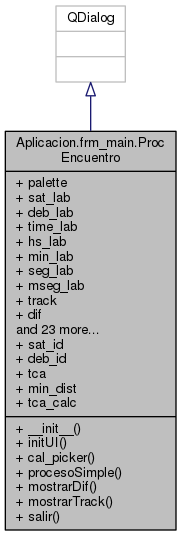
\includegraphics[width=252pt]{class_aplicacion_1_1frm__main_1_1_proc_encuentro__inherit__graph}
\end{center}
\end{figure}


\-Collaboration diagram for \-Aplicacion.\-frm\-\_\-main.\-Proc\-Encuentro\-:\nopagebreak
\begin{figure}[H]
\begin{center}
\leavevmode
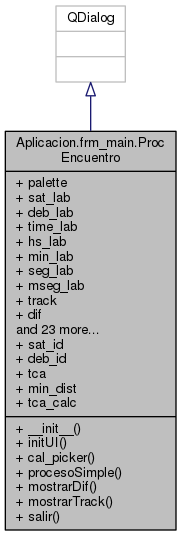
\includegraphics[width=252pt]{class_aplicacion_1_1frm__main_1_1_proc_encuentro__coll__graph}
\end{center}
\end{figure}
\subsection*{\-Public \-Member \-Functions}
\begin{DoxyCompactItemize}
\item 
def {\bf \-\_\-\-\_\-init\-\_\-\-\_\-}
\item 
def {\bf init\-U\-I}
\item 
def {\bf proceso\-Simple}
\item 
def {\bf mostrar\-Dif}
\item 
def {\bf mostrar\-Track}
\item 
def {\bf salir}
\end{DoxyCompactItemize}
\subsection*{\-Public \-Attributes}
\begin{DoxyCompactItemize}
\item 
{\bf palette}
\item 
{\bf sat\-\_\-lab}
\item 
{\bf deb\-\_\-lab}
\item 
{\bf time\-\_\-lab}
\item 
{\bf hs\-\_\-lab}
\item 
{\bf min\-\_\-lab}
\item 
{\bf seg\-\_\-lab}
\item 
{\bf mseg\-\_\-lab}
\item 
{\bf track}
\item 
{\bf dif}
\item 
{\bf boton\-\_\-carga\-\_\-fecha}
\item 
{\bf boton\-\_\-encuetro}
\item 
{\bf boton\-\_\-dif}
\item 
{\bf boton\-\_\-track}
\item 
{\bf boton\-\_\-salir}
\item 
{\bf sat\-\_\-id\-\_\-text}
\item 
{\bf deb\-\_\-id\-\_\-text}
\item 
{\bf tca\-\_\-text}
\item 
{\bf hs\-\_\-tex}
\item 
{\bf min\-\_\-tex}
\item 
{\bf seg\-\_\-tex}
\item 
{\bf mseg\-\_\-tex}
\item 
{\bf table\-Encuentro}
\item 
{\bf hora}
\item 
{\bf cal}
\item 
{\bf fecha}
\item 
{\bf horas}
\item 
{\bf tca}
\item 
{\bf sat\-\_\-id}
\item 
{\bf deb\-\_\-id}
\item 
{\bf n}
\item 
{\bf min\-\_\-dist}
\item 
{\bf tca\-\_\-calc}
\item 
{\bf ma\-\_\-comb}
\item 
{\bf poc\-\_\-arx}
\item 
{\bf archivo\-\_\-dif}
\item 
{\bf grafico\-\_\-dif}
\item 
{\bf pixmap1}
\item 
{\bf track\-\_\-graf}
\end{DoxyCompactItemize}


\subsection{\-Detailed \-Description}


\-Definition at line 322 of file frm\-\_\-main.\-py.



\subsection{\-Constructor \& \-Destructor \-Documentation}
\index{\-Aplicacion\-::frm\-\_\-main\-::\-Proc\-Encuentro@{\-Aplicacion\-::frm\-\_\-main\-::\-Proc\-Encuentro}!\-\_\-\-\_\-init\-\_\-\-\_\-@{\-\_\-\-\_\-init\-\_\-\-\_\-}}
\index{\-\_\-\-\_\-init\-\_\-\-\_\-@{\-\_\-\-\_\-init\-\_\-\-\_\-}!Aplicacion::frm_main::ProcEncuentro@{\-Aplicacion\-::frm\-\_\-main\-::\-Proc\-Encuentro}}
\subsubsection[{\-\_\-\-\_\-init\-\_\-\-\_\-}]{\setlength{\rightskip}{0pt plus 5cm}def {\bf \-Aplicacion.\-frm\-\_\-main.\-Proc\-Encuentro.\-\_\-\-\_\-init\-\_\-\-\_\-} (
\begin{DoxyParamCaption}
\item[{}]{self, }
\item[{}]{parent = {\ttfamily \-None}}
\end{DoxyParamCaption}
)}\label{class_aplicacion_1_1frm__main_1_1_proc_encuentro_abf26f68ed41e5b2a3802baf0dafbace2}


\-Definition at line 323 of file frm\-\_\-main.\-py.


\begin{DoxyCode}
323 
324     def __init__(self,parent=None):
325         QDialog.__init__(self,parent)
326 
327         self.setWindowModality(Qt.ApplicationModal)
        self.initUI()
\end{DoxyCode}


\-Here is the call graph for this function\-:\nopagebreak
\begin{figure}[H]
\begin{center}
\leavevmode
\includegraphics[width=350pt]{class_aplicacion_1_1frm__main_1_1_proc_encuentro_abf26f68ed41e5b2a3802baf0dafbace2_cgraph}
\end{center}
\end{figure}




\subsection{\-Member \-Function \-Documentation}
\index{\-Aplicacion\-::frm\-\_\-main\-::\-Proc\-Encuentro@{\-Aplicacion\-::frm\-\_\-main\-::\-Proc\-Encuentro}!init\-U\-I@{init\-U\-I}}
\index{init\-U\-I@{init\-U\-I}!Aplicacion::frm_main::ProcEncuentro@{\-Aplicacion\-::frm\-\_\-main\-::\-Proc\-Encuentro}}
\subsubsection[{init\-U\-I}]{\setlength{\rightskip}{0pt plus 5cm}def {\bf \-Aplicacion.\-frm\-\_\-main.\-Proc\-Encuentro.\-init\-U\-I} (
\begin{DoxyParamCaption}
\item[{}]{self}
\end{DoxyParamCaption}
)}\label{class_aplicacion_1_1frm__main_1_1_proc_encuentro_a0df5f10ce0e6544ee7996b2ffd32d5c3}


\-Definition at line 335 of file frm\-\_\-main.\-py.


\begin{DoxyCode}
335 
336     def initUI(self):
337         self.palette = QPalette()
338         self.palette.setColor(QPalette.Background,Qt.white)
339         self.setPalette(self.palette)
340         
341         """
342         Etiquetas
343         """
344         self.sat_lab  = QLabel('Satelite NORAD ID')
345         self.deb_lab  = QLabel('Desecho NORAD ID')
346         self.time_lab = QLabel('TCA')
347         self.hs_lab   = QLabel('Hs:')
348         self.min_lab  = QLabel('min:')
349         self.seg_lab  = QLabel('seg')
350         self.mseg_lab = QLabel('mseg')
351         # imagen 
352         self.track = QLabel() 
353         self.dif   = QLabel()
354         """
355         Botones
356         """
357         self.boton_carga_fecha  = QPushButton('Cargar')
358         self.boton_encuetro = QPushButton('Procesar Encuentro')
359         self.boton_dif      = QPushButton('Ver diferencias')
360         self.boton_track    = QPushButton('Track')
361         self.boton_salir    = QPushButton('Salir')
362         """
363         Campos de Edicion
364         """
365         self.sat_id_text = QLineEdit()
366         self.deb_id_text = QLineEdit() 
367         # calendario
368         # nice widget for editing the date  
369         self.tca_text    = QDateEdit()  
370         self.tca_text.setCalendarPopup(True)
371 
372 #         self.fecha = self.tca_text.selectedDate()
373 #        self.tca_text    = QCalendarWidget()
374         self.hs_tex      = QLineEdit()
375         self.min_tex     = QLineEdit()
376         self.seg_tex     = QLineEdit()
377         self.mseg_tex    = QLineEdit()
378         """
379         Otros
380         """
381         self.tableEncuentro   = QTableWidget()
382         self.tableEncuentro.setRowCount(1)
383         self.tableEncuentro.setColumnCount(5)
384         listaLabels=['Norad Id','Nombre','TCAarx','MinD arx','PoC']
385         self.tableEncuentro.setHorizontalHeaderLabels(listaLabels)      
386 #       # Fecha y Hora
387         self.hora = QTimeEdit()
388 #       self.hora.setTime(QTime(19,14,11))
389         """
390         Plantilla
391         """
392         grid = QGridLayout()
393         grid.setSpacing(5)
394         scroll = QScrollArea()
395 
396         grid.addWidget(self.sat_lab,2,1)
397         grid.addWidget(self.sat_id_text,2,2)
398         grid.addWidget(self.deb_lab,3,1)
399         grid.addWidget(self.deb_id_text,3,2)
400         grid.addWidget(self.time_lab,4,1)
401 #        grid.addWidget(self.tca_text,4,2)
402         grid.addWidget(self.tca_text,4,2)
403         grid.addWidget(self.hora,5,2)
404         grid.addWidget(self.boton_carga_fecha,5,1)
405 #         grid.addWidget(self.hs_tex,4,3)
406 #         grid.addWidget(self.hs_lab,4,4)
407 #         grid.addWidget(self.min_tex,4,5)
408 #         grid.addWidget(self.min_lab,4,6)
409 #         grid.addWidget(self.seg_tex,4,7)
410 #         grid.addWidget(self.seg_lab,4,8)
411 #         grid.addWidget(self.mseg_tex,4,9)
412 #         grid.addWidget(self.mseg_lab,4,10)        
413         grid.addWidget(self.tableEncuentro,8,1,2,5)
414         grid.addWidget(self.track,2,3,5,3)
415         grid.addWidget(self.dif,12,4)
416         grid.addWidget(self.boton_encuetro,10,10)
417         grid.addWidget(self.boton_dif,11,10)
418         grid.addWidget(self.boton_track,12,10)
419         grid.addWidget(self.boton_salir,13,10)
420         """
421         Acciones
422         """
423         self.boton_encuetro.clicked.connect(self.procesoSimple)
424         self.boton_salir.clicked.connect(self.salir)
425         self.boton_track.clicked.connect(self.mostrarTrack)
426         self.boton_dif.clicked.connect(self.mostrarDif)
427         self.boton_track.setEnabled(False)
428         self.boton_dif.setEnabled(False)
429 
430         self.setLayout(grid)
431         self.setWindowTitle('Procesamiento de Encuentro')    
432         self.show()

\end{DoxyCode}


\-Here is the caller graph for this function\-:\nopagebreak
\begin{figure}[H]
\begin{center}
\leavevmode
\includegraphics[width=350pt]{class_aplicacion_1_1frm__main_1_1_proc_encuentro_a0df5f10ce0e6544ee7996b2ffd32d5c3_icgraph}
\end{center}
\end{figure}


\index{\-Aplicacion\-::frm\-\_\-main\-::\-Proc\-Encuentro@{\-Aplicacion\-::frm\-\_\-main\-::\-Proc\-Encuentro}!mostrar\-Dif@{mostrar\-Dif}}
\index{mostrar\-Dif@{mostrar\-Dif}!Aplicacion::frm_main::ProcEncuentro@{\-Aplicacion\-::frm\-\_\-main\-::\-Proc\-Encuentro}}
\subsubsection[{mostrar\-Dif}]{\setlength{\rightskip}{0pt plus 5cm}def {\bf \-Aplicacion.\-frm\-\_\-main.\-Proc\-Encuentro.\-mostrar\-Dif} (
\begin{DoxyParamCaption}
\item[{}]{self}
\end{DoxyParamCaption}
)}\label{class_aplicacion_1_1frm__main_1_1_proc_encuentro_a05cf641959fca6add2fc6bd39742c972}


\-Definition at line 489 of file frm\-\_\-main.\-py.


\begin{DoxyCode}
489 
490     def mostrarDif(self):
491         self.grafico_dif= ploteos.grafica_diferenciasRIC(self.archivo_dif)
492         self.pixmap1 = QPixmap(self.grafico_dif)
493         self.dif.setPixmap(self.pixmap1)
    
\end{DoxyCode}
\index{\-Aplicacion\-::frm\-\_\-main\-::\-Proc\-Encuentro@{\-Aplicacion\-::frm\-\_\-main\-::\-Proc\-Encuentro}!mostrar\-Track@{mostrar\-Track}}
\index{mostrar\-Track@{mostrar\-Track}!Aplicacion::frm_main::ProcEncuentro@{\-Aplicacion\-::frm\-\_\-main\-::\-Proc\-Encuentro}}
\subsubsection[{mostrar\-Track}]{\setlength{\rightskip}{0pt plus 5cm}def {\bf \-Aplicacion.\-frm\-\_\-main.\-Proc\-Encuentro.\-mostrar\-Track} (
\begin{DoxyParamCaption}
\item[{}]{self}
\end{DoxyParamCaption}
)}\label{class_aplicacion_1_1frm__main_1_1_proc_encuentro_a48160da57694ee4375e6b0fdd7a99a71}


\-Definition at line 494 of file frm\-\_\-main.\-py.


\begin{DoxyCode}
494 
495     def mostrarTrack(self):
496         self.track_graf = QPixmap('../visual/archivos/ploteo_track.ps')
497         self.track.setPixmap( self.track_graf)
        
\end{DoxyCode}
\index{\-Aplicacion\-::frm\-\_\-main\-::\-Proc\-Encuentro@{\-Aplicacion\-::frm\-\_\-main\-::\-Proc\-Encuentro}!proceso\-Simple@{proceso\-Simple}}
\index{proceso\-Simple@{proceso\-Simple}!Aplicacion::frm_main::ProcEncuentro@{\-Aplicacion\-::frm\-\_\-main\-::\-Proc\-Encuentro}}
\subsubsection[{proceso\-Simple}]{\setlength{\rightskip}{0pt plus 5cm}def {\bf \-Aplicacion.\-frm\-\_\-main.\-Proc\-Encuentro.\-proceso\-Simple} (
\begin{DoxyParamCaption}
\item[{}]{self}
\end{DoxyParamCaption}
)}\label{class_aplicacion_1_1frm__main_1_1_proc_encuentro_a361d53a30428a61d5fd92d34d4b4000f}
\begin{DoxyVerb}
Propaga los objetos involucrados un intervalos [tca-90:tca+10]
Calcula:
    Miss Distance
    TCA calculado
    Diferencias en RTN ---> Plotea.
    Genera archivo lat, long ---> Plotea.          
\end{DoxyVerb}
 

\-Definition at line 433 of file frm\-\_\-main.\-py.


\begin{DoxyCode}
433 
434     def procesoSimple(self):
435         """
436         Propaga los objetos involucrados un intervalos [tca-90:tca+10]
437         Calcula:
438             Miss Distance
439             TCA calculado
440             Diferencias en RTN ---> Plotea.
441             Genera archivo lat, long ---> Plotea.          
442         """
443 
444         self.cal = self.tca_text.calendarWidget()
445         self.fecha = self.cal.selectedDate().toPyDate()
446         self.horas = self.hora.time()
447         self.tca = QDateTime(self.fecha,self.horas).toPyDateTime()
448 
449 #         # Importar los TLE de NORAD.    
450         self.sat_id=str(self.sat_id_text.text())
451         self.deb_id=str(self.deb_id_text.text())
452 #         hs =int(self.hs_tex.text())
453 #         min=int(self.min_tex.text())
454 #         seg=int(self.seg_tex.text())
455 #         fecha = self.tca_text.selectedDate()#.toPyDate()
456 #         hora = QTime(hs,min,seg)
457 #       
       self.tca=datetime(2004,9,2,19,14,11)#QDateTime(fecha,hora).toPyDateTime()
458         tle_sat=Tle.creadoxParam(self.sat_id, self.tca)
459         tle_deb=Tle.creadoxParam(self.deb_id, self.tca)
460 #         
461         """
462         Propagacion hasta el Encuentro
463         """
464         self.n=3
465         encuentro1=Encuentro(tle_sat,tle_deb,self.tca,self.n)
466         self.min_dist= encuentro1.mod_minDist
467         self.tca_calc= encuentro1.tca_c
468         self.ma_comb= encuentro1.calculaMacombinada()
469         self.poc_arx=encuentro1.calculaPoC_circ()
470         self.tableEncuentro.setItem(0,0, QTableWidgetItem(self.sat_id))
471         self.tableEncuentro.setItem(0,1, QTableWidgetItem(self.deb_id))
472         self.tableEncuentro.setItem(0,2, QTableWidgetItem(datetime.strftime(
      self.tca_calc,'%Y-%m-%d %H:%M:%S')))
473         self.tableEncuentro.setItem(0,3, QTableWidgetItem(str(round(self.
      min_dist,7))))
474         self.tableEncuentro.setItem(0,4, QTableWidgetItem(str(round(self.poc_arx
      ,7))))
475         # formato de tabla
476         header = self.tableEncuentro.horizontalHeader()
477         header.setResizeMode(0,QHeaderView.Stretch)
478         header.setResizeMode(1,QHeaderView.ResizeToContents)
479         header.setResizeMode(2,QHeaderView.ResizeToContents)
480         header.setResizeMode(3,QHeaderView.ResizeToContents)
481         # archivo de diferencias.
482         self.archivo_dif=encuentro1.archivo_dif
483         print 'Minima Distancia = ', encuentro1.mod_minDist,encuentro1.
      epoca_ini
484         grafica_track('../Encuentro/archivos/'+str(self.sat_id)+'U', '
      ../Encuentro/archivos/'+str(self.deb_id)+'U')
485         print 'fin del procesamiento.'
486        
487         self.boton_track.setEnabled(True)
488         self.boton_dif.setEnabled(True)
    
\end{DoxyCode}
\index{\-Aplicacion\-::frm\-\_\-main\-::\-Proc\-Encuentro@{\-Aplicacion\-::frm\-\_\-main\-::\-Proc\-Encuentro}!salir@{salir}}
\index{salir@{salir}!Aplicacion::frm_main::ProcEncuentro@{\-Aplicacion\-::frm\-\_\-main\-::\-Proc\-Encuentro}}
\subsubsection[{salir}]{\setlength{\rightskip}{0pt plus 5cm}def {\bf \-Aplicacion.\-frm\-\_\-main.\-Proc\-Encuentro.\-salir} (
\begin{DoxyParamCaption}
\item[{}]{self}
\end{DoxyParamCaption}
)}\label{class_aplicacion_1_1frm__main_1_1_proc_encuentro_a58cb9bc6a82da02c73bbee45fce6a4d4}


\-Definition at line 498 of file frm\-\_\-main.\-py.


\begin{DoxyCode}
498 
499     def salir(self):
500         self.accept()    
501         
        
\end{DoxyCode}


\subsection{\-Member \-Data \-Documentation}
\index{\-Aplicacion\-::frm\-\_\-main\-::\-Proc\-Encuentro@{\-Aplicacion\-::frm\-\_\-main\-::\-Proc\-Encuentro}!archivo\-\_\-dif@{archivo\-\_\-dif}}
\index{archivo\-\_\-dif@{archivo\-\_\-dif}!Aplicacion::frm_main::ProcEncuentro@{\-Aplicacion\-::frm\-\_\-main\-::\-Proc\-Encuentro}}
\subsubsection[{archivo\-\_\-dif}]{\setlength{\rightskip}{0pt plus 5cm}{\bf \-Aplicacion\-::frm\-\_\-main.\-Proc\-Encuentro\-::archivo\-\_\-dif}}\label{class_aplicacion_1_1frm__main_1_1_proc_encuentro_ad91f138c2d34ec1dddfa274961d9f4b9}


\-Definition at line 447 of file frm\-\_\-main.\-py.

\index{\-Aplicacion\-::frm\-\_\-main\-::\-Proc\-Encuentro@{\-Aplicacion\-::frm\-\_\-main\-::\-Proc\-Encuentro}!boton\-\_\-carga\-\_\-fecha@{boton\-\_\-carga\-\_\-fecha}}
\index{boton\-\_\-carga\-\_\-fecha@{boton\-\_\-carga\-\_\-fecha}!Aplicacion::frm_main::ProcEncuentro@{\-Aplicacion\-::frm\-\_\-main\-::\-Proc\-Encuentro}}
\subsubsection[{boton\-\_\-carga\-\_\-fecha}]{\setlength{\rightskip}{0pt plus 5cm}{\bf \-Aplicacion\-::frm\-\_\-main.\-Proc\-Encuentro\-::boton\-\_\-carga\-\_\-fecha}}\label{class_aplicacion_1_1frm__main_1_1_proc_encuentro_ad65d0ac83d7deb549f0e4bd83d834a3e}


\-Definition at line 339 of file frm\-\_\-main.\-py.

\index{\-Aplicacion\-::frm\-\_\-main\-::\-Proc\-Encuentro@{\-Aplicacion\-::frm\-\_\-main\-::\-Proc\-Encuentro}!boton\-\_\-dif@{boton\-\_\-dif}}
\index{boton\-\_\-dif@{boton\-\_\-dif}!Aplicacion::frm_main::ProcEncuentro@{\-Aplicacion\-::frm\-\_\-main\-::\-Proc\-Encuentro}}
\subsubsection[{boton\-\_\-dif}]{\setlength{\rightskip}{0pt plus 5cm}{\bf \-Aplicacion\-::frm\-\_\-main.\-Proc\-Encuentro\-::boton\-\_\-dif}}\label{class_aplicacion_1_1frm__main_1_1_proc_encuentro_aeb31ca7f82f7239731383b96e7075337}


\-Definition at line 339 of file frm\-\_\-main.\-py.

\index{\-Aplicacion\-::frm\-\_\-main\-::\-Proc\-Encuentro@{\-Aplicacion\-::frm\-\_\-main\-::\-Proc\-Encuentro}!boton\-\_\-encuetro@{boton\-\_\-encuetro}}
\index{boton\-\_\-encuetro@{boton\-\_\-encuetro}!Aplicacion::frm_main::ProcEncuentro@{\-Aplicacion\-::frm\-\_\-main\-::\-Proc\-Encuentro}}
\subsubsection[{boton\-\_\-encuetro}]{\setlength{\rightskip}{0pt plus 5cm}{\bf \-Aplicacion\-::frm\-\_\-main.\-Proc\-Encuentro\-::boton\-\_\-encuetro}}\label{class_aplicacion_1_1frm__main_1_1_proc_encuentro_a8644605ee796fee24b6dd923fc266846}


\-Definition at line 339 of file frm\-\_\-main.\-py.

\index{\-Aplicacion\-::frm\-\_\-main\-::\-Proc\-Encuentro@{\-Aplicacion\-::frm\-\_\-main\-::\-Proc\-Encuentro}!boton\-\_\-salir@{boton\-\_\-salir}}
\index{boton\-\_\-salir@{boton\-\_\-salir}!Aplicacion::frm_main::ProcEncuentro@{\-Aplicacion\-::frm\-\_\-main\-::\-Proc\-Encuentro}}
\subsubsection[{boton\-\_\-salir}]{\setlength{\rightskip}{0pt plus 5cm}{\bf \-Aplicacion\-::frm\-\_\-main.\-Proc\-Encuentro\-::boton\-\_\-salir}}\label{class_aplicacion_1_1frm__main_1_1_proc_encuentro_aca036cbd7f766bf701ae36c2a5a7b3b8}


\-Definition at line 339 of file frm\-\_\-main.\-py.

\index{\-Aplicacion\-::frm\-\_\-main\-::\-Proc\-Encuentro@{\-Aplicacion\-::frm\-\_\-main\-::\-Proc\-Encuentro}!boton\-\_\-track@{boton\-\_\-track}}
\index{boton\-\_\-track@{boton\-\_\-track}!Aplicacion::frm_main::ProcEncuentro@{\-Aplicacion\-::frm\-\_\-main\-::\-Proc\-Encuentro}}
\subsubsection[{boton\-\_\-track}]{\setlength{\rightskip}{0pt plus 5cm}{\bf \-Aplicacion\-::frm\-\_\-main.\-Proc\-Encuentro\-::boton\-\_\-track}}\label{class_aplicacion_1_1frm__main_1_1_proc_encuentro_a1941629b003e80f8ded4df0f456c7bd2}


\-Definition at line 339 of file frm\-\_\-main.\-py.

\index{\-Aplicacion\-::frm\-\_\-main\-::\-Proc\-Encuentro@{\-Aplicacion\-::frm\-\_\-main\-::\-Proc\-Encuentro}!cal@{cal}}
\index{cal@{cal}!Aplicacion::frm_main::ProcEncuentro@{\-Aplicacion\-::frm\-\_\-main\-::\-Proc\-Encuentro}}
\subsubsection[{cal}]{\setlength{\rightskip}{0pt plus 5cm}{\bf \-Aplicacion\-::frm\-\_\-main.\-Proc\-Encuentro\-::cal}}\label{class_aplicacion_1_1frm__main_1_1_proc_encuentro_ac7468fc1228d26d5ea967897aa0c2d19}


\-Definition at line 440 of file frm\-\_\-main.\-py.

\index{\-Aplicacion\-::frm\-\_\-main\-::\-Proc\-Encuentro@{\-Aplicacion\-::frm\-\_\-main\-::\-Proc\-Encuentro}!deb\-\_\-id@{deb\-\_\-id}}
\index{deb\-\_\-id@{deb\-\_\-id}!Aplicacion::frm_main::ProcEncuentro@{\-Aplicacion\-::frm\-\_\-main\-::\-Proc\-Encuentro}}
\subsubsection[{deb\-\_\-id}]{\setlength{\rightskip}{0pt plus 5cm}{\bf \-Aplicacion\-::frm\-\_\-main.\-Proc\-Encuentro\-::deb\-\_\-id}}\label{class_aplicacion_1_1frm__main_1_1_proc_encuentro_a29b4b7477eec45dc43c8420fe57f380b}


\-Definition at line 440 of file frm\-\_\-main.\-py.

\index{\-Aplicacion\-::frm\-\_\-main\-::\-Proc\-Encuentro@{\-Aplicacion\-::frm\-\_\-main\-::\-Proc\-Encuentro}!deb\-\_\-id\-\_\-text@{deb\-\_\-id\-\_\-text}}
\index{deb\-\_\-id\-\_\-text@{deb\-\_\-id\-\_\-text}!Aplicacion::frm_main::ProcEncuentro@{\-Aplicacion\-::frm\-\_\-main\-::\-Proc\-Encuentro}}
\subsubsection[{deb\-\_\-id\-\_\-text}]{\setlength{\rightskip}{0pt plus 5cm}{\bf \-Aplicacion\-::frm\-\_\-main.\-Proc\-Encuentro\-::deb\-\_\-id\-\_\-text}}\label{class_aplicacion_1_1frm__main_1_1_proc_encuentro_a2f2e7ac9884884073150132b5a7fee63}


\-Definition at line 341 of file frm\-\_\-main.\-py.

\index{\-Aplicacion\-::frm\-\_\-main\-::\-Proc\-Encuentro@{\-Aplicacion\-::frm\-\_\-main\-::\-Proc\-Encuentro}!deb\-\_\-lab@{deb\-\_\-lab}}
\index{deb\-\_\-lab@{deb\-\_\-lab}!Aplicacion::frm_main::ProcEncuentro@{\-Aplicacion\-::frm\-\_\-main\-::\-Proc\-Encuentro}}
\subsubsection[{deb\-\_\-lab}]{\setlength{\rightskip}{0pt plus 5cm}{\bf \-Aplicacion\-::frm\-\_\-main.\-Proc\-Encuentro\-::deb\-\_\-lab}}\label{class_aplicacion_1_1frm__main_1_1_proc_encuentro_ab4c6985a68b1ffe2180b3b88489b06aa}


\-Definition at line 337 of file frm\-\_\-main.\-py.

\index{\-Aplicacion\-::frm\-\_\-main\-::\-Proc\-Encuentro@{\-Aplicacion\-::frm\-\_\-main\-::\-Proc\-Encuentro}!dif@{dif}}
\index{dif@{dif}!Aplicacion::frm_main::ProcEncuentro@{\-Aplicacion\-::frm\-\_\-main\-::\-Proc\-Encuentro}}
\subsubsection[{dif}]{\setlength{\rightskip}{0pt plus 5cm}{\bf \-Aplicacion\-::frm\-\_\-main.\-Proc\-Encuentro\-::dif}}\label{class_aplicacion_1_1frm__main_1_1_proc_encuentro_a9bdbd42721fd4c57a52c8370e4d75a8b}


\-Definition at line 337 of file frm\-\_\-main.\-py.

\index{\-Aplicacion\-::frm\-\_\-main\-::\-Proc\-Encuentro@{\-Aplicacion\-::frm\-\_\-main\-::\-Proc\-Encuentro}!fecha@{fecha}}
\index{fecha@{fecha}!Aplicacion::frm_main::ProcEncuentro@{\-Aplicacion\-::frm\-\_\-main\-::\-Proc\-Encuentro}}
\subsubsection[{fecha}]{\setlength{\rightskip}{0pt plus 5cm}{\bf \-Aplicacion\-::frm\-\_\-main.\-Proc\-Encuentro\-::fecha}}\label{class_aplicacion_1_1frm__main_1_1_proc_encuentro_a817571257a62cf7e3738720dc7cbc8e6}


\-Definition at line 440 of file frm\-\_\-main.\-py.

\index{\-Aplicacion\-::frm\-\_\-main\-::\-Proc\-Encuentro@{\-Aplicacion\-::frm\-\_\-main\-::\-Proc\-Encuentro}!grafico\-\_\-dif@{grafico\-\_\-dif}}
\index{grafico\-\_\-dif@{grafico\-\_\-dif}!Aplicacion::frm_main::ProcEncuentro@{\-Aplicacion\-::frm\-\_\-main\-::\-Proc\-Encuentro}}
\subsubsection[{grafico\-\_\-dif}]{\setlength{\rightskip}{0pt plus 5cm}{\bf \-Aplicacion\-::frm\-\_\-main.\-Proc\-Encuentro\-::grafico\-\_\-dif}}\label{class_aplicacion_1_1frm__main_1_1_proc_encuentro_a21cd8515b488cb5a1a7ed05f7a02ac28}


\-Definition at line 489 of file frm\-\_\-main.\-py.

\index{\-Aplicacion\-::frm\-\_\-main\-::\-Proc\-Encuentro@{\-Aplicacion\-::frm\-\_\-main\-::\-Proc\-Encuentro}!hora@{hora}}
\index{hora@{hora}!Aplicacion::frm_main::ProcEncuentro@{\-Aplicacion\-::frm\-\_\-main\-::\-Proc\-Encuentro}}
\subsubsection[{hora}]{\setlength{\rightskip}{0pt plus 5cm}{\bf \-Aplicacion\-::frm\-\_\-main.\-Proc\-Encuentro\-::hora}}\label{class_aplicacion_1_1frm__main_1_1_proc_encuentro_a6bafebd8e2e4f63e64a7fbb7a5f47e41}


\-Definition at line 344 of file frm\-\_\-main.\-py.

\index{\-Aplicacion\-::frm\-\_\-main\-::\-Proc\-Encuentro@{\-Aplicacion\-::frm\-\_\-main\-::\-Proc\-Encuentro}!horas@{horas}}
\index{horas@{horas}!Aplicacion::frm_main::ProcEncuentro@{\-Aplicacion\-::frm\-\_\-main\-::\-Proc\-Encuentro}}
\subsubsection[{horas}]{\setlength{\rightskip}{0pt plus 5cm}{\bf \-Aplicacion\-::frm\-\_\-main.\-Proc\-Encuentro\-::horas}}\label{class_aplicacion_1_1frm__main_1_1_proc_encuentro_a46d50b0d81fb2a57756f583dbe2fb0e5}


\-Definition at line 440 of file frm\-\_\-main.\-py.

\index{\-Aplicacion\-::frm\-\_\-main\-::\-Proc\-Encuentro@{\-Aplicacion\-::frm\-\_\-main\-::\-Proc\-Encuentro}!hs\-\_\-lab@{hs\-\_\-lab}}
\index{hs\-\_\-lab@{hs\-\_\-lab}!Aplicacion::frm_main::ProcEncuentro@{\-Aplicacion\-::frm\-\_\-main\-::\-Proc\-Encuentro}}
\subsubsection[{hs\-\_\-lab}]{\setlength{\rightskip}{0pt plus 5cm}{\bf \-Aplicacion\-::frm\-\_\-main.\-Proc\-Encuentro\-::hs\-\_\-lab}}\label{class_aplicacion_1_1frm__main_1_1_proc_encuentro_a27ad8a3bf2a7faab4b19e36c1d790dfa}


\-Definition at line 337 of file frm\-\_\-main.\-py.

\index{\-Aplicacion\-::frm\-\_\-main\-::\-Proc\-Encuentro@{\-Aplicacion\-::frm\-\_\-main\-::\-Proc\-Encuentro}!hs\-\_\-tex@{hs\-\_\-tex}}
\index{hs\-\_\-tex@{hs\-\_\-tex}!Aplicacion::frm_main::ProcEncuentro@{\-Aplicacion\-::frm\-\_\-main\-::\-Proc\-Encuentro}}
\subsubsection[{hs\-\_\-tex}]{\setlength{\rightskip}{0pt plus 5cm}{\bf \-Aplicacion\-::frm\-\_\-main.\-Proc\-Encuentro\-::hs\-\_\-tex}}\label{class_aplicacion_1_1frm__main_1_1_proc_encuentro_a47af2e4568d0c0103808db6f86817885}


\-Definition at line 342 of file frm\-\_\-main.\-py.

\index{\-Aplicacion\-::frm\-\_\-main\-::\-Proc\-Encuentro@{\-Aplicacion\-::frm\-\_\-main\-::\-Proc\-Encuentro}!ma\-\_\-comb@{ma\-\_\-comb}}
\index{ma\-\_\-comb@{ma\-\_\-comb}!Aplicacion::frm_main::ProcEncuentro@{\-Aplicacion\-::frm\-\_\-main\-::\-Proc\-Encuentro}}
\subsubsection[{ma\-\_\-comb}]{\setlength{\rightskip}{0pt plus 5cm}{\bf \-Aplicacion\-::frm\-\_\-main.\-Proc\-Encuentro\-::ma\-\_\-comb}}\label{class_aplicacion_1_1frm__main_1_1_proc_encuentro_a0c27a291d5a87b4cb0d8a2aafc939aca}


\-Definition at line 447 of file frm\-\_\-main.\-py.

\index{\-Aplicacion\-::frm\-\_\-main\-::\-Proc\-Encuentro@{\-Aplicacion\-::frm\-\_\-main\-::\-Proc\-Encuentro}!min\-\_\-dist@{min\-\_\-dist}}
\index{min\-\_\-dist@{min\-\_\-dist}!Aplicacion::frm_main::ProcEncuentro@{\-Aplicacion\-::frm\-\_\-main\-::\-Proc\-Encuentro}}
\subsubsection[{min\-\_\-dist}]{\setlength{\rightskip}{0pt plus 5cm}{\bf \-Aplicacion\-::frm\-\_\-main.\-Proc\-Encuentro\-::min\-\_\-dist}}\label{class_aplicacion_1_1frm__main_1_1_proc_encuentro_a8071ddf9f15d916a95ba4937e00c02bc}


\-Definition at line 447 of file frm\-\_\-main.\-py.

\index{\-Aplicacion\-::frm\-\_\-main\-::\-Proc\-Encuentro@{\-Aplicacion\-::frm\-\_\-main\-::\-Proc\-Encuentro}!min\-\_\-lab@{min\-\_\-lab}}
\index{min\-\_\-lab@{min\-\_\-lab}!Aplicacion::frm_main::ProcEncuentro@{\-Aplicacion\-::frm\-\_\-main\-::\-Proc\-Encuentro}}
\subsubsection[{min\-\_\-lab}]{\setlength{\rightskip}{0pt plus 5cm}{\bf \-Aplicacion\-::frm\-\_\-main.\-Proc\-Encuentro\-::min\-\_\-lab}}\label{class_aplicacion_1_1frm__main_1_1_proc_encuentro_a775f0c0c1b4e7d4e68fdf04efa135071}


\-Definition at line 337 of file frm\-\_\-main.\-py.

\index{\-Aplicacion\-::frm\-\_\-main\-::\-Proc\-Encuentro@{\-Aplicacion\-::frm\-\_\-main\-::\-Proc\-Encuentro}!min\-\_\-tex@{min\-\_\-tex}}
\index{min\-\_\-tex@{min\-\_\-tex}!Aplicacion::frm_main::ProcEncuentro@{\-Aplicacion\-::frm\-\_\-main\-::\-Proc\-Encuentro}}
\subsubsection[{min\-\_\-tex}]{\setlength{\rightskip}{0pt plus 5cm}{\bf \-Aplicacion\-::frm\-\_\-main.\-Proc\-Encuentro\-::min\-\_\-tex}}\label{class_aplicacion_1_1frm__main_1_1_proc_encuentro_ad30a0e55f3288798e84da8aadb8e3bcd}


\-Definition at line 342 of file frm\-\_\-main.\-py.

\index{\-Aplicacion\-::frm\-\_\-main\-::\-Proc\-Encuentro@{\-Aplicacion\-::frm\-\_\-main\-::\-Proc\-Encuentro}!mseg\-\_\-lab@{mseg\-\_\-lab}}
\index{mseg\-\_\-lab@{mseg\-\_\-lab}!Aplicacion::frm_main::ProcEncuentro@{\-Aplicacion\-::frm\-\_\-main\-::\-Proc\-Encuentro}}
\subsubsection[{mseg\-\_\-lab}]{\setlength{\rightskip}{0pt plus 5cm}{\bf \-Aplicacion\-::frm\-\_\-main.\-Proc\-Encuentro\-::mseg\-\_\-lab}}\label{class_aplicacion_1_1frm__main_1_1_proc_encuentro_a35b3a9db8e7eae867df6d9e7762dfea0}


\-Definition at line 337 of file frm\-\_\-main.\-py.

\index{\-Aplicacion\-::frm\-\_\-main\-::\-Proc\-Encuentro@{\-Aplicacion\-::frm\-\_\-main\-::\-Proc\-Encuentro}!mseg\-\_\-tex@{mseg\-\_\-tex}}
\index{mseg\-\_\-tex@{mseg\-\_\-tex}!Aplicacion::frm_main::ProcEncuentro@{\-Aplicacion\-::frm\-\_\-main\-::\-Proc\-Encuentro}}
\subsubsection[{mseg\-\_\-tex}]{\setlength{\rightskip}{0pt plus 5cm}{\bf \-Aplicacion\-::frm\-\_\-main.\-Proc\-Encuentro\-::mseg\-\_\-tex}}\label{class_aplicacion_1_1frm__main_1_1_proc_encuentro_afe9a3882b2c5537df85cb18df916f01b}


\-Definition at line 342 of file frm\-\_\-main.\-py.

\index{\-Aplicacion\-::frm\-\_\-main\-::\-Proc\-Encuentro@{\-Aplicacion\-::frm\-\_\-main\-::\-Proc\-Encuentro}!n@{n}}
\index{n@{n}!Aplicacion::frm_main::ProcEncuentro@{\-Aplicacion\-::frm\-\_\-main\-::\-Proc\-Encuentro}}
\subsubsection[{n}]{\setlength{\rightskip}{0pt plus 5cm}{\bf \-Aplicacion\-::frm\-\_\-main.\-Proc\-Encuentro\-::n}}\label{class_aplicacion_1_1frm__main_1_1_proc_encuentro_aeaa64f1663476183b0bd3a2241277eeb}


\-Definition at line 447 of file frm\-\_\-main.\-py.

\index{\-Aplicacion\-::frm\-\_\-main\-::\-Proc\-Encuentro@{\-Aplicacion\-::frm\-\_\-main\-::\-Proc\-Encuentro}!palette@{palette}}
\index{palette@{palette}!Aplicacion::frm_main::ProcEncuentro@{\-Aplicacion\-::frm\-\_\-main\-::\-Proc\-Encuentro}}
\subsubsection[{palette}]{\setlength{\rightskip}{0pt plus 5cm}{\bf \-Aplicacion\-::frm\-\_\-main.\-Proc\-Encuentro\-::palette}}\label{class_aplicacion_1_1frm__main_1_1_proc_encuentro_acf473733b894ad6506a589a393363799}


\-Definition at line 335 of file frm\-\_\-main.\-py.

\index{\-Aplicacion\-::frm\-\_\-main\-::\-Proc\-Encuentro@{\-Aplicacion\-::frm\-\_\-main\-::\-Proc\-Encuentro}!pixmap1@{pixmap1}}
\index{pixmap1@{pixmap1}!Aplicacion::frm_main::ProcEncuentro@{\-Aplicacion\-::frm\-\_\-main\-::\-Proc\-Encuentro}}
\subsubsection[{pixmap1}]{\setlength{\rightskip}{0pt plus 5cm}{\bf \-Aplicacion\-::frm\-\_\-main.\-Proc\-Encuentro\-::pixmap1}}\label{class_aplicacion_1_1frm__main_1_1_proc_encuentro_af0da3467b8af9d808e55ff06ef69bdc2}


\-Definition at line 489 of file frm\-\_\-main.\-py.

\index{\-Aplicacion\-::frm\-\_\-main\-::\-Proc\-Encuentro@{\-Aplicacion\-::frm\-\_\-main\-::\-Proc\-Encuentro}!poc\-\_\-arx@{poc\-\_\-arx}}
\index{poc\-\_\-arx@{poc\-\_\-arx}!Aplicacion::frm_main::ProcEncuentro@{\-Aplicacion\-::frm\-\_\-main\-::\-Proc\-Encuentro}}
\subsubsection[{poc\-\_\-arx}]{\setlength{\rightskip}{0pt plus 5cm}{\bf \-Aplicacion\-::frm\-\_\-main.\-Proc\-Encuentro\-::poc\-\_\-arx}}\label{class_aplicacion_1_1frm__main_1_1_proc_encuentro_abb41a1dfa6b16c3548805933b92a5f9f}


\-Definition at line 447 of file frm\-\_\-main.\-py.

\index{\-Aplicacion\-::frm\-\_\-main\-::\-Proc\-Encuentro@{\-Aplicacion\-::frm\-\_\-main\-::\-Proc\-Encuentro}!sat\-\_\-id@{sat\-\_\-id}}
\index{sat\-\_\-id@{sat\-\_\-id}!Aplicacion::frm_main::ProcEncuentro@{\-Aplicacion\-::frm\-\_\-main\-::\-Proc\-Encuentro}}
\subsubsection[{sat\-\_\-id}]{\setlength{\rightskip}{0pt plus 5cm}{\bf \-Aplicacion\-::frm\-\_\-main.\-Proc\-Encuentro\-::sat\-\_\-id}}\label{class_aplicacion_1_1frm__main_1_1_proc_encuentro_aa2733a045e28eb7c02115a09d51a836a}


\-Definition at line 440 of file frm\-\_\-main.\-py.

\index{\-Aplicacion\-::frm\-\_\-main\-::\-Proc\-Encuentro@{\-Aplicacion\-::frm\-\_\-main\-::\-Proc\-Encuentro}!sat\-\_\-id\-\_\-text@{sat\-\_\-id\-\_\-text}}
\index{sat\-\_\-id\-\_\-text@{sat\-\_\-id\-\_\-text}!Aplicacion::frm_main::ProcEncuentro@{\-Aplicacion\-::frm\-\_\-main\-::\-Proc\-Encuentro}}
\subsubsection[{sat\-\_\-id\-\_\-text}]{\setlength{\rightskip}{0pt plus 5cm}{\bf \-Aplicacion\-::frm\-\_\-main.\-Proc\-Encuentro\-::sat\-\_\-id\-\_\-text}}\label{class_aplicacion_1_1frm__main_1_1_proc_encuentro_a2007df02bfb5112b366cfc4328c280a7}


\-Definition at line 341 of file frm\-\_\-main.\-py.

\index{\-Aplicacion\-::frm\-\_\-main\-::\-Proc\-Encuentro@{\-Aplicacion\-::frm\-\_\-main\-::\-Proc\-Encuentro}!sat\-\_\-lab@{sat\-\_\-lab}}
\index{sat\-\_\-lab@{sat\-\_\-lab}!Aplicacion::frm_main::ProcEncuentro@{\-Aplicacion\-::frm\-\_\-main\-::\-Proc\-Encuentro}}
\subsubsection[{sat\-\_\-lab}]{\setlength{\rightskip}{0pt plus 5cm}{\bf \-Aplicacion\-::frm\-\_\-main.\-Proc\-Encuentro\-::sat\-\_\-lab}}\label{class_aplicacion_1_1frm__main_1_1_proc_encuentro_a9d2a1d34deb3175ecf73d0dfe65242f6}


\-Definition at line 337 of file frm\-\_\-main.\-py.

\index{\-Aplicacion\-::frm\-\_\-main\-::\-Proc\-Encuentro@{\-Aplicacion\-::frm\-\_\-main\-::\-Proc\-Encuentro}!seg\-\_\-lab@{seg\-\_\-lab}}
\index{seg\-\_\-lab@{seg\-\_\-lab}!Aplicacion::frm_main::ProcEncuentro@{\-Aplicacion\-::frm\-\_\-main\-::\-Proc\-Encuentro}}
\subsubsection[{seg\-\_\-lab}]{\setlength{\rightskip}{0pt plus 5cm}{\bf \-Aplicacion\-::frm\-\_\-main.\-Proc\-Encuentro\-::seg\-\_\-lab}}\label{class_aplicacion_1_1frm__main_1_1_proc_encuentro_ab3d01094156d3614f263c6f42d6febd7}


\-Definition at line 337 of file frm\-\_\-main.\-py.

\index{\-Aplicacion\-::frm\-\_\-main\-::\-Proc\-Encuentro@{\-Aplicacion\-::frm\-\_\-main\-::\-Proc\-Encuentro}!seg\-\_\-tex@{seg\-\_\-tex}}
\index{seg\-\_\-tex@{seg\-\_\-tex}!Aplicacion::frm_main::ProcEncuentro@{\-Aplicacion\-::frm\-\_\-main\-::\-Proc\-Encuentro}}
\subsubsection[{seg\-\_\-tex}]{\setlength{\rightskip}{0pt plus 5cm}{\bf \-Aplicacion\-::frm\-\_\-main.\-Proc\-Encuentro\-::seg\-\_\-tex}}\label{class_aplicacion_1_1frm__main_1_1_proc_encuentro_aa8a995a723c03140e4a348b4ad2ab417}


\-Definition at line 342 of file frm\-\_\-main.\-py.

\index{\-Aplicacion\-::frm\-\_\-main\-::\-Proc\-Encuentro@{\-Aplicacion\-::frm\-\_\-main\-::\-Proc\-Encuentro}!table\-Encuentro@{table\-Encuentro}}
\index{table\-Encuentro@{table\-Encuentro}!Aplicacion::frm_main::ProcEncuentro@{\-Aplicacion\-::frm\-\_\-main\-::\-Proc\-Encuentro}}
\subsubsection[{table\-Encuentro}]{\setlength{\rightskip}{0pt plus 5cm}{\bf \-Aplicacion\-::frm\-\_\-main.\-Proc\-Encuentro\-::table\-Encuentro}}\label{class_aplicacion_1_1frm__main_1_1_proc_encuentro_a8480361e1e7806f47f338b7df37e33bc}


\-Definition at line 344 of file frm\-\_\-main.\-py.

\index{\-Aplicacion\-::frm\-\_\-main\-::\-Proc\-Encuentro@{\-Aplicacion\-::frm\-\_\-main\-::\-Proc\-Encuentro}!tca@{tca}}
\index{tca@{tca}!Aplicacion::frm_main::ProcEncuentro@{\-Aplicacion\-::frm\-\_\-main\-::\-Proc\-Encuentro}}
\subsubsection[{tca}]{\setlength{\rightskip}{0pt plus 5cm}{\bf \-Aplicacion\-::frm\-\_\-main.\-Proc\-Encuentro\-::tca}}\label{class_aplicacion_1_1frm__main_1_1_proc_encuentro_a197eac71261a31914e870a5d4d61c40c}


\-Definition at line 440 of file frm\-\_\-main.\-py.

\index{\-Aplicacion\-::frm\-\_\-main\-::\-Proc\-Encuentro@{\-Aplicacion\-::frm\-\_\-main\-::\-Proc\-Encuentro}!tca\-\_\-calc@{tca\-\_\-calc}}
\index{tca\-\_\-calc@{tca\-\_\-calc}!Aplicacion::frm_main::ProcEncuentro@{\-Aplicacion\-::frm\-\_\-main\-::\-Proc\-Encuentro}}
\subsubsection[{tca\-\_\-calc}]{\setlength{\rightskip}{0pt plus 5cm}{\bf \-Aplicacion\-::frm\-\_\-main.\-Proc\-Encuentro\-::tca\-\_\-calc}}\label{class_aplicacion_1_1frm__main_1_1_proc_encuentro_a975e5f4e68911fb69a242157bc1450ab}


\-Definition at line 447 of file frm\-\_\-main.\-py.

\index{\-Aplicacion\-::frm\-\_\-main\-::\-Proc\-Encuentro@{\-Aplicacion\-::frm\-\_\-main\-::\-Proc\-Encuentro}!tca\-\_\-text@{tca\-\_\-text}}
\index{tca\-\_\-text@{tca\-\_\-text}!Aplicacion::frm_main::ProcEncuentro@{\-Aplicacion\-::frm\-\_\-main\-::\-Proc\-Encuentro}}
\subsubsection[{tca\-\_\-text}]{\setlength{\rightskip}{0pt plus 5cm}{\bf \-Aplicacion\-::frm\-\_\-main.\-Proc\-Encuentro\-::tca\-\_\-text}}\label{class_aplicacion_1_1frm__main_1_1_proc_encuentro_a92e586584e7eed72d3aadf7e67695439}


\-Definition at line 341 of file frm\-\_\-main.\-py.

\index{\-Aplicacion\-::frm\-\_\-main\-::\-Proc\-Encuentro@{\-Aplicacion\-::frm\-\_\-main\-::\-Proc\-Encuentro}!time\-\_\-lab@{time\-\_\-lab}}
\index{time\-\_\-lab@{time\-\_\-lab}!Aplicacion::frm_main::ProcEncuentro@{\-Aplicacion\-::frm\-\_\-main\-::\-Proc\-Encuentro}}
\subsubsection[{time\-\_\-lab}]{\setlength{\rightskip}{0pt plus 5cm}{\bf \-Aplicacion\-::frm\-\_\-main.\-Proc\-Encuentro\-::time\-\_\-lab}}\label{class_aplicacion_1_1frm__main_1_1_proc_encuentro_a241a5287aae2adf3fa66aee1ade8ad22}


\-Definition at line 337 of file frm\-\_\-main.\-py.

\index{\-Aplicacion\-::frm\-\_\-main\-::\-Proc\-Encuentro@{\-Aplicacion\-::frm\-\_\-main\-::\-Proc\-Encuentro}!track@{track}}
\index{track@{track}!Aplicacion::frm_main::ProcEncuentro@{\-Aplicacion\-::frm\-\_\-main\-::\-Proc\-Encuentro}}
\subsubsection[{track}]{\setlength{\rightskip}{0pt plus 5cm}{\bf \-Aplicacion\-::frm\-\_\-main.\-Proc\-Encuentro\-::track}}\label{class_aplicacion_1_1frm__main_1_1_proc_encuentro_a5aad2c5d4f711da0c77ad9a0e2b4f568}


\-Definition at line 337 of file frm\-\_\-main.\-py.

\index{\-Aplicacion\-::frm\-\_\-main\-::\-Proc\-Encuentro@{\-Aplicacion\-::frm\-\_\-main\-::\-Proc\-Encuentro}!track\-\_\-graf@{track\-\_\-graf}}
\index{track\-\_\-graf@{track\-\_\-graf}!Aplicacion::frm_main::ProcEncuentro@{\-Aplicacion\-::frm\-\_\-main\-::\-Proc\-Encuentro}}
\subsubsection[{track\-\_\-graf}]{\setlength{\rightskip}{0pt plus 5cm}{\bf \-Aplicacion\-::frm\-\_\-main.\-Proc\-Encuentro\-::track\-\_\-graf}}\label{class_aplicacion_1_1frm__main_1_1_proc_encuentro_abf2a27956c7c1831b3cbe373bf6419b1}


\-Definition at line 494 of file frm\-\_\-main.\-py.



\-The documentation for this class was generated from the following file\-:\begin{DoxyCompactItemize}
\item 
\-Aplicacion/{\bf frm\-\_\-main.\-py}\end{DoxyCompactItemize}

\section{\-Aplicacion.\-frm\-\_\-main.\-Proc\-Mision \-Class \-Reference}
\label{class_aplicacion_1_1frm__main_1_1_proc_mision}\index{\-Aplicacion.\-frm\-\_\-main.\-Proc\-Mision@{\-Aplicacion.\-frm\-\_\-main.\-Proc\-Mision}}


\-Inheritance diagram for \-Aplicacion.\-frm\-\_\-main.\-Proc\-Mision\-:\nopagebreak
\begin{figure}[H]
\begin{center}
\leavevmode
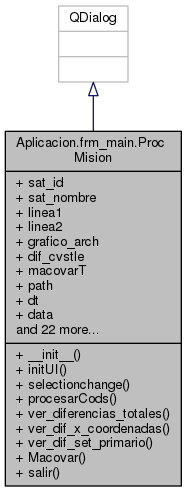
\includegraphics[width=236pt]{class_aplicacion_1_1frm__main_1_1_proc_mision__inherit__graph}
\end{center}
\end{figure}


\-Collaboration diagram for \-Aplicacion.\-frm\-\_\-main.\-Proc\-Mision\-:\nopagebreak
\begin{figure}[H]
\begin{center}
\leavevmode
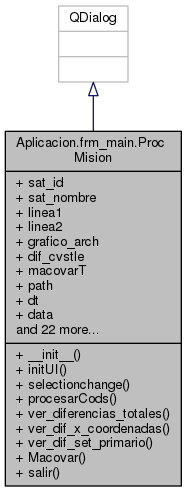
\includegraphics[width=236pt]{class_aplicacion_1_1frm__main_1_1_proc_mision__coll__graph}
\end{center}
\end{figure}
\subsection*{\-Public \-Member \-Functions}
\begin{DoxyCompactItemize}
\item 
def {\bf \-\_\-\-\_\-init\-\_\-\-\_\-}
\item 
def {\bf init\-U\-I}
\item 
def {\bf selectionchange}
\item 
def {\bf procesar\-Cods}
\item 
def {\bf ver\-\_\-diferencias\-\_\-totales}
\item 
def {\bf ver\-\_\-dif\-\_\-x\-\_\-coordenadas}
\item 
def {\bf ver\-\_\-dif\-\_\-set\-\_\-primario}
\item 
def {\bf \-Macovar}
\item 
def {\bf salir}
\end{DoxyCompactItemize}
\subsection*{\-Public \-Attributes}
\begin{DoxyCompactItemize}
\item 
{\bf sat\-\_\-id}
\item 
{\bf sat\-\_\-nombre}
\item 
{\bf linea1}
\item 
{\bf linea2}
\item 
{\bf grafico\-\_\-arch}
\item 
{\bf dif\-\_\-cvstle}
\item 
{\bf macovar\-T}
\item 
{\bf path}
\item 
{\bf dt}
\item 
{\bf data}
\item 
{\bf set\-\_\-datos15dias}
\item 
{\bf coef}
\item 
{\bf set\-\_\-datos}
\item 
{\bf grilla}
\item 
{\bf mision\-\_\-lab}
\item 
{\bf fechaini\-\_\-lab}
\item 
{\bf fechafin\-\_\-lab}
\item 
{\bf ma\-\_\-lab}
\item 
{\bf boton\-\_\-procesar}
\item 
{\bf boton\-\_\-dtotales}
\item 
{\bf boton\-\_\-dxcoord}
\item 
{\bf boton\-\_\-dsetprimario}
\item 
{\bf boton\-\_\-macovar}
\item 
{\bf boton\-\_\-salir}
\item 
{\bf fechaini\-\_\-edit}
\item 
{\bf fechafin\-\_\-edit}
\item 
{\bf tlepri\-\_\-edit}
\item 
{\bf lista\-Sat}
\item 
{\bf table\-View}
\item 
{\bf dic\-\_\-satelites}
\item 
{\bf fini}
\item 
{\bf ffin}
\end{DoxyCompactItemize}


\subsection{\-Detailed \-Description}
\begin{DoxyVerb}
REQUIERE CORRER PRIMERO EL PROCESAMIENTO TLE!!!
Utiliza los datos ya cargados en TleAdmin/tle y los Datos de los archivos CODS.
Carga el set de datos TLE y realiza el metodo de Osweiler para estimar las diferenicas
\end{DoxyVerb}
 

\-Definition at line 928 of file frm\-\_\-main.\-py.



\subsection{\-Constructor \& \-Destructor \-Documentation}
\index{\-Aplicacion\-::frm\-\_\-main\-::\-Proc\-Mision@{\-Aplicacion\-::frm\-\_\-main\-::\-Proc\-Mision}!\-\_\-\-\_\-init\-\_\-\-\_\-@{\-\_\-\-\_\-init\-\_\-\-\_\-}}
\index{\-\_\-\-\_\-init\-\_\-\-\_\-@{\-\_\-\-\_\-init\-\_\-\-\_\-}!Aplicacion::frm_main::ProcMision@{\-Aplicacion\-::frm\-\_\-main\-::\-Proc\-Mision}}
\subsubsection[{\-\_\-\-\_\-init\-\_\-\-\_\-}]{\setlength{\rightskip}{0pt plus 5cm}def {\bf \-Aplicacion.\-frm\-\_\-main.\-Proc\-Mision.\-\_\-\-\_\-init\-\_\-\-\_\-} (
\begin{DoxyParamCaption}
\item[{}]{self, }
\item[{}]{parent = {\ttfamily \-None}}
\end{DoxyParamCaption}
)}\label{class_aplicacion_1_1frm__main_1_1_proc_mision_ab386f8a70670aa3edd2ff232d0c9696d}


\-Definition at line 935 of file frm\-\_\-main.\-py.


\begin{DoxyCode}
935 
936     def __init__(self,parent=None):
937         QDialog.__init__(self,parent)
938 
939         self.setWindowModality(Qt.ApplicationModal)
940 #       self.resize(1200, 600)
941 #        self.resize(1700, 700)
942         self.initUI()
943         
944         self.sat_id='99999'
945         self.sat_nombre=''
946         self.linea1=''
947         self.linea2=''
948         self.grafico_arch=''
949         self.dif_cvstle= ''
950         self.macovarT=''
951         self.path='../Comparar/diferencias/'
952         self.dt=[]
953         self.data=[]
954         self.set_datos15dias=[]
955         self.coef=[]
956         self.set_datos=[]
        
\end{DoxyCode}


\subsection{\-Member \-Function \-Documentation}
\index{\-Aplicacion\-::frm\-\_\-main\-::\-Proc\-Mision@{\-Aplicacion\-::frm\-\_\-main\-::\-Proc\-Mision}!init\-U\-I@{init\-U\-I}}
\index{init\-U\-I@{init\-U\-I}!Aplicacion::frm_main::ProcMision@{\-Aplicacion\-::frm\-\_\-main\-::\-Proc\-Mision}}
\subsubsection[{init\-U\-I}]{\setlength{\rightskip}{0pt plus 5cm}def {\bf \-Aplicacion.\-frm\-\_\-main.\-Proc\-Mision.\-init\-U\-I} (
\begin{DoxyParamCaption}
\item[{}]{self}
\end{DoxyParamCaption}
)}\label{class_aplicacion_1_1frm__main_1_1_proc_mision_a9218bf963132eaa32d23247740787305}


\-Definition at line 957 of file frm\-\_\-main.\-py.


\begin{DoxyCode}
957 
958     def initUI(self):
959         self.grilla = QGridLayout()
960         self.grilla.setSpacing(10)
961         
962         """
963         Etiquetas
964         """
965         self.mision_lab     = QLabel('Mision')
966         self.fechaini_lab   = QLabel('Fecha Inicio')
967         self.fechafin_lab   = QLabel('Fecha Fin')
968         self.ma_lab       = QLabel('Ma. Varianza-Covarianza')
969         
970         """
971         Botones
972         """
973         self.boton_procesar     = QPushButton('Procesar')
974         self.boton_dtotales     = QPushButton('Graficar Diferencias Totales')
975         self.boton_dxcoord      = QPushButton('Graficar Diferencias por
       Coordenadas')
976         self.boton_dsetprimario = QPushButton ('Graficar Diferencias del Set
       primario')
977         self.boton_macovar      = QPushButton('Calcular Matriz')
978         self.boton_salir        = QPushButton('Salir')
979         
980         """
981         Campos de Edicion
982         """
983         self.fechaini_edit   = QLineEdit()
984         self.fechafin_edit   = QLineEdit()
985         self.tlepri_edit     = QTextEdit()
986                 
987         """
988         Lista desplegada
989         """
990         self.listaSat       = QComboBox()
991         self.listaSat.addItem("...");
992         self.listaSat.addItem("SAC-D"); 
993         self.listaSat.addItem("LAGEOS");
994         self.listaSat.addItem("ICESAT");
995         """
996         tabla
997         """
998         self.tableView       = QTableWidget()
999         
1000         self.grilla.addWidget(self.mision_lab,1,0)
1001         self.grilla.addWidget(self.listaSat,1,1)
1002         self.grilla.addWidget(self.boton_procesar,2,1)
1003         self.grilla.addWidget(self.fechaini_lab,3,0)
1004         self.grilla.addWidget(self.fechaini_edit,3,1)
1005         self.grilla.addWidget(self.fechafin_lab,4,0)
1006         self.grilla.addWidget(self.fechafin_edit,4,1)
1007         self.grilla.addWidget(self.tlepri_edit,5,0,1,2)
1008         self.grilla.addWidget(self.boton_dtotales,6,0)
1009         self.grilla.addWidget(self.boton_dxcoord,6,1)
1010         self.grilla.addWidget(self.boton_dsetprimario,6,2)
1011         self.grilla.addWidget(self.tableView,7,0,7,1)
1012         self.grilla.addWidget(self.boton_macovar,8,1)
1013         self.grilla.addWidget(self.boton_salir,17,1)
1014         
1015         """
1016         Acciones
1017         """
1018         self.listaSat.currentIndexChanged.connect(self.selectionchange)
1019         self.boton_procesar.clicked.connect(self.procesarCods)
1020         self.boton_procesar.setEnabled(False)
1021         self.boton_dtotales.setEnabled(False)
1022         self.boton_dxcoord.setEnabled(False)
1023         self.boton_dsetprimario.setEnabled(False)
1024         self.boton_macovar.setEnabled(False)
1025         self.boton_salir.clicked.connect(self.salir)
1026         self.boton_dtotales.clicked.connect(self.ver_diferencias_totales)
1027         self.boton_dxcoord.clicked.connect(self.ver_dif_x_coordenadas)
1028         self.boton_dsetprimario.clicked.connect(self.ver_dif_set_primario)
1029         self.boton_macovar.clicked.connect(self.Macovar)
1030 #        self.datos_mis_edit.textChanged.connect(self.validar_nombre)
1031                 
1032         self.setWindowTitle('PROCESAMIENTO de DATOS CODS')
1033         self.setLayout(self.grilla) 
        
\end{DoxyCode}
\index{\-Aplicacion\-::frm\-\_\-main\-::\-Proc\-Mision@{\-Aplicacion\-::frm\-\_\-main\-::\-Proc\-Mision}!\-Macovar@{\-Macovar}}
\index{\-Macovar@{\-Macovar}!Aplicacion::frm_main::ProcMision@{\-Aplicacion\-::frm\-\_\-main\-::\-Proc\-Mision}}
\subsubsection[{\-Macovar}]{\setlength{\rightskip}{0pt plus 5cm}def {\bf \-Aplicacion.\-frm\-\_\-main.\-Proc\-Mision.\-Macovar} (
\begin{DoxyParamCaption}
\item[{}]{self}
\end{DoxyParamCaption}
)}\label{class_aplicacion_1_1frm__main_1_1_proc_mision_acc3e51ea01f718127f28f752079417d2}


\-Definition at line 1074 of file frm\-\_\-main.\-py.


\begin{DoxyCode}
1074 
1075     def Macovar(self):
1076         self.macovarT=EjecutaMaCovarCODS(self.grafico_arch)
1077         self.tableView.setRowCount(len(self.macovarT))
1078         self.tableView.setColumnCount(len(self.macovarT))
1079         for i,fila in enumerate(self.macovarT):
1080             for j,col in enumerate(fila):
1081                 self.tableView.setItem(i,j,QTableWidgetItem(str(col)))
   
\end{DoxyCode}


\-Here is the call graph for this function\-:\nopagebreak
\begin{figure}[H]
\begin{center}
\leavevmode
\includegraphics[width=350pt]{class_aplicacion_1_1frm__main_1_1_proc_mision_acc3e51ea01f718127f28f752079417d2_cgraph}
\end{center}
\end{figure}


\index{\-Aplicacion\-::frm\-\_\-main\-::\-Proc\-Mision@{\-Aplicacion\-::frm\-\_\-main\-::\-Proc\-Mision}!procesar\-Cods@{procesar\-Cods}}
\index{procesar\-Cods@{procesar\-Cods}!Aplicacion::frm_main::ProcMision@{\-Aplicacion\-::frm\-\_\-main\-::\-Proc\-Mision}}
\subsubsection[{procesar\-Cods}]{\setlength{\rightskip}{0pt plus 5cm}def {\bf \-Aplicacion.\-frm\-\_\-main.\-Proc\-Mision.\-procesar\-Cods} (
\begin{DoxyParamCaption}
\item[{}]{self}
\end{DoxyParamCaption}
)}\label{class_aplicacion_1_1frm__main_1_1_proc_mision_a833aec7ff42fabde02e729e5ab5e5a44}


\-Definition at line 1040 of file frm\-\_\-main.\-py.


\begin{DoxyCode}
1040 
1041     def procesarCods(self):
1042         files=glob.glob('../Comparar/diferencias/*')
1043         for filename in files:
1044             os.unlink(filename)
1045 #        self.set_datos =ejecutaProcesamientoCods()
1046         self.set_datos= dif_tleCODS15dias()
1047         self.sat_id=self.set_datos[0]
1048         self.linea1=self.set_datos[1]
1049         self.linea2=self.set_datos[2]
1050         self.fini=self.set_datos[3]
1051         self.ffin=self.set_datos[4]
1052         self.dt=self.set_datos[5]
1053         self.data=self.set_datos[6]
1054         self.coef=self.set_datos[7]
1055         self.grafico_arch=self.set_datos[8]
1056         self.fechaini_edit.setText(self.fini)
1057         self.fechafin_edit.setText(self.ffin)
1058         self.tlepri_edit.setText(self.linea1+'\n'+self.linea2)
1059         self.boton_dtotales.setEnabled(True)
1060         self.boton_dxcoord.setEnabled(True)
1061         self.boton_dsetprimario.setEnabled(True)
1062         self.boton_macovar.setEnabled(True)
        
\end{DoxyCode}


\-Here is the call graph for this function\-:\nopagebreak
\begin{figure}[H]
\begin{center}
\leavevmode
\includegraphics[width=350pt]{class_aplicacion_1_1frm__main_1_1_proc_mision_a833aec7ff42fabde02e729e5ab5e5a44_cgraph}
\end{center}
\end{figure}


\index{\-Aplicacion\-::frm\-\_\-main\-::\-Proc\-Mision@{\-Aplicacion\-::frm\-\_\-main\-::\-Proc\-Mision}!salir@{salir}}
\index{salir@{salir}!Aplicacion::frm_main::ProcMision@{\-Aplicacion\-::frm\-\_\-main\-::\-Proc\-Mision}}
\subsubsection[{salir}]{\setlength{\rightskip}{0pt plus 5cm}def {\bf \-Aplicacion.\-frm\-\_\-main.\-Proc\-Mision.\-salir} (
\begin{DoxyParamCaption}
\item[{}]{self}
\end{DoxyParamCaption}
)}\label{class_aplicacion_1_1frm__main_1_1_proc_mision_abe5eaa272c4758f505193a0359e13b7e}


\-Definition at line 1082 of file frm\-\_\-main.\-py.


\begin{DoxyCode}
1082 
1083     def salir(self):
1084         self.accept()
1085         
1086         
#def IniciaApp():
\end{DoxyCode}
\index{\-Aplicacion\-::frm\-\_\-main\-::\-Proc\-Mision@{\-Aplicacion\-::frm\-\_\-main\-::\-Proc\-Mision}!selectionchange@{selectionchange}}
\index{selectionchange@{selectionchange}!Aplicacion::frm_main::ProcMision@{\-Aplicacion\-::frm\-\_\-main\-::\-Proc\-Mision}}
\subsubsection[{selectionchange}]{\setlength{\rightskip}{0pt plus 5cm}def {\bf \-Aplicacion.\-frm\-\_\-main.\-Proc\-Mision.\-selectionchange} (
\begin{DoxyParamCaption}
\item[{}]{self, }
\item[{}]{i}
\end{DoxyParamCaption}
)}\label{class_aplicacion_1_1frm__main_1_1_proc_mision_a32dded3405be1a68a86b698ab03077ae}


\-Definition at line 1034 of file frm\-\_\-main.\-py.


\begin{DoxyCode}
1034 
1035     def selectionchange(self,i):
1036         self.sat_nombre= self.listaSat.currentText()
1037         self.dic_satelites={'SAC-D':37673,'LAGEOS':8820,'ICESAT':27642}
1038         self.sat_id=self.dic_satelites[str(self.sat_nombre)]
1039         self.boton_procesar.setEnabled(True)
        
\end{DoxyCode}
\index{\-Aplicacion\-::frm\-\_\-main\-::\-Proc\-Mision@{\-Aplicacion\-::frm\-\_\-main\-::\-Proc\-Mision}!ver\-\_\-dif\-\_\-set\-\_\-primario@{ver\-\_\-dif\-\_\-set\-\_\-primario}}
\index{ver\-\_\-dif\-\_\-set\-\_\-primario@{ver\-\_\-dif\-\_\-set\-\_\-primario}!Aplicacion::frm_main::ProcMision@{\-Aplicacion\-::frm\-\_\-main\-::\-Proc\-Mision}}
\subsubsection[{ver\-\_\-dif\-\_\-set\-\_\-primario}]{\setlength{\rightskip}{0pt plus 5cm}def {\bf \-Aplicacion.\-frm\-\_\-main.\-Proc\-Mision.\-ver\-\_\-dif\-\_\-set\-\_\-primario} (
\begin{DoxyParamCaption}
\item[{}]{self}
\end{DoxyParamCaption}
)}\label{class_aplicacion_1_1frm__main_1_1_proc_mision_ae8b8bd169d4cb3383b04eef230662d94}


\-Definition at line 1069 of file frm\-\_\-main.\-py.


\begin{DoxyCode}
1069 
1070     def ver_dif_set_primario(self):
1071         ploteos.grafica_set15dias(self.data, self.coef)
1072 #       
       ploteos.grafica_set_principal(self.sat_id,self.path,self.grafico_arch,self.ffin)
1073         
        
\end{DoxyCode}
\index{\-Aplicacion\-::frm\-\_\-main\-::\-Proc\-Mision@{\-Aplicacion\-::frm\-\_\-main\-::\-Proc\-Mision}!ver\-\_\-dif\-\_\-x\-\_\-coordenadas@{ver\-\_\-dif\-\_\-x\-\_\-coordenadas}}
\index{ver\-\_\-dif\-\_\-x\-\_\-coordenadas@{ver\-\_\-dif\-\_\-x\-\_\-coordenadas}!Aplicacion::frm_main::ProcMision@{\-Aplicacion\-::frm\-\_\-main\-::\-Proc\-Mision}}
\subsubsection[{ver\-\_\-dif\-\_\-x\-\_\-coordenadas}]{\setlength{\rightskip}{0pt plus 5cm}def {\bf \-Aplicacion.\-frm\-\_\-main.\-Proc\-Mision.\-ver\-\_\-dif\-\_\-x\-\_\-coordenadas} (
\begin{DoxyParamCaption}
\item[{}]{self}
\end{DoxyParamCaption}
)}\label{class_aplicacion_1_1frm__main_1_1_proc_mision_a75e87bed4ae6deeb7c2a537e7aec92c2}


\-Definition at line 1066 of file frm\-\_\-main.\-py.


\begin{DoxyCode}
1066 
1067     def ver_dif_x_coordenadas(self):
1068         ploteos.grafica_setcompleto(self.sat_id,self.path,self.data, self.coef)
        
\end{DoxyCode}
\index{\-Aplicacion\-::frm\-\_\-main\-::\-Proc\-Mision@{\-Aplicacion\-::frm\-\_\-main\-::\-Proc\-Mision}!ver\-\_\-diferencias\-\_\-totales@{ver\-\_\-diferencias\-\_\-totales}}
\index{ver\-\_\-diferencias\-\_\-totales@{ver\-\_\-diferencias\-\_\-totales}!Aplicacion::frm_main::ProcMision@{\-Aplicacion\-::frm\-\_\-main\-::\-Proc\-Mision}}
\subsubsection[{ver\-\_\-diferencias\-\_\-totales}]{\setlength{\rightskip}{0pt plus 5cm}def {\bf \-Aplicacion.\-frm\-\_\-main.\-Proc\-Mision.\-ver\-\_\-diferencias\-\_\-totales} (
\begin{DoxyParamCaption}
\item[{}]{self}
\end{DoxyParamCaption}
)}\label{class_aplicacion_1_1frm__main_1_1_proc_mision_a1f554257b2dc3c7d9205fcccc4567503}


\-Definition at line 1063 of file frm\-\_\-main.\-py.


\begin{DoxyCode}
1063 
1064     def ver_diferencias_totales(self):
1065         ploteos.grafica_diferenciasTotales(self.sat_id,self.path,self.data,
      self.coef)
        
\end{DoxyCode}


\subsection{\-Member \-Data \-Documentation}
\index{\-Aplicacion\-::frm\-\_\-main\-::\-Proc\-Mision@{\-Aplicacion\-::frm\-\_\-main\-::\-Proc\-Mision}!boton\-\_\-dsetprimario@{boton\-\_\-dsetprimario}}
\index{boton\-\_\-dsetprimario@{boton\-\_\-dsetprimario}!Aplicacion::frm_main::ProcMision@{\-Aplicacion\-::frm\-\_\-main\-::\-Proc\-Mision}}
\subsubsection[{boton\-\_\-dsetprimario}]{\setlength{\rightskip}{0pt plus 5cm}{\bf \-Aplicacion\-::frm\-\_\-main.\-Proc\-Mision\-::boton\-\_\-dsetprimario}}\label{class_aplicacion_1_1frm__main_1_1_proc_mision_a55df2c2f9f6fcc71be77878a2dd313d7}


\-Definition at line 961 of file frm\-\_\-main.\-py.

\index{\-Aplicacion\-::frm\-\_\-main\-::\-Proc\-Mision@{\-Aplicacion\-::frm\-\_\-main\-::\-Proc\-Mision}!boton\-\_\-dtotales@{boton\-\_\-dtotales}}
\index{boton\-\_\-dtotales@{boton\-\_\-dtotales}!Aplicacion::frm_main::ProcMision@{\-Aplicacion\-::frm\-\_\-main\-::\-Proc\-Mision}}
\subsubsection[{boton\-\_\-dtotales}]{\setlength{\rightskip}{0pt plus 5cm}{\bf \-Aplicacion\-::frm\-\_\-main.\-Proc\-Mision\-::boton\-\_\-dtotales}}\label{class_aplicacion_1_1frm__main_1_1_proc_mision_a42d8a8b34d3c480ab348894c322a860c}


\-Definition at line 961 of file frm\-\_\-main.\-py.

\index{\-Aplicacion\-::frm\-\_\-main\-::\-Proc\-Mision@{\-Aplicacion\-::frm\-\_\-main\-::\-Proc\-Mision}!boton\-\_\-dxcoord@{boton\-\_\-dxcoord}}
\index{boton\-\_\-dxcoord@{boton\-\_\-dxcoord}!Aplicacion::frm_main::ProcMision@{\-Aplicacion\-::frm\-\_\-main\-::\-Proc\-Mision}}
\subsubsection[{boton\-\_\-dxcoord}]{\setlength{\rightskip}{0pt plus 5cm}{\bf \-Aplicacion\-::frm\-\_\-main.\-Proc\-Mision\-::boton\-\_\-dxcoord}}\label{class_aplicacion_1_1frm__main_1_1_proc_mision_a4cf737219230bd140c671f40ad1c14bc}


\-Definition at line 961 of file frm\-\_\-main.\-py.

\index{\-Aplicacion\-::frm\-\_\-main\-::\-Proc\-Mision@{\-Aplicacion\-::frm\-\_\-main\-::\-Proc\-Mision}!boton\-\_\-macovar@{boton\-\_\-macovar}}
\index{boton\-\_\-macovar@{boton\-\_\-macovar}!Aplicacion::frm_main::ProcMision@{\-Aplicacion\-::frm\-\_\-main\-::\-Proc\-Mision}}
\subsubsection[{boton\-\_\-macovar}]{\setlength{\rightskip}{0pt plus 5cm}{\bf \-Aplicacion\-::frm\-\_\-main.\-Proc\-Mision\-::boton\-\_\-macovar}}\label{class_aplicacion_1_1frm__main_1_1_proc_mision_a92c0069fe00775eefd9f1f233ad40635}


\-Definition at line 961 of file frm\-\_\-main.\-py.

\index{\-Aplicacion\-::frm\-\_\-main\-::\-Proc\-Mision@{\-Aplicacion\-::frm\-\_\-main\-::\-Proc\-Mision}!boton\-\_\-procesar@{boton\-\_\-procesar}}
\index{boton\-\_\-procesar@{boton\-\_\-procesar}!Aplicacion::frm_main::ProcMision@{\-Aplicacion\-::frm\-\_\-main\-::\-Proc\-Mision}}
\subsubsection[{boton\-\_\-procesar}]{\setlength{\rightskip}{0pt plus 5cm}{\bf \-Aplicacion\-::frm\-\_\-main.\-Proc\-Mision\-::boton\-\_\-procesar}}\label{class_aplicacion_1_1frm__main_1_1_proc_mision_ad25186a3caaabdf09c46f5b8260a3e4a}


\-Definition at line 961 of file frm\-\_\-main.\-py.

\index{\-Aplicacion\-::frm\-\_\-main\-::\-Proc\-Mision@{\-Aplicacion\-::frm\-\_\-main\-::\-Proc\-Mision}!boton\-\_\-salir@{boton\-\_\-salir}}
\index{boton\-\_\-salir@{boton\-\_\-salir}!Aplicacion::frm_main::ProcMision@{\-Aplicacion\-::frm\-\_\-main\-::\-Proc\-Mision}}
\subsubsection[{boton\-\_\-salir}]{\setlength{\rightskip}{0pt plus 5cm}{\bf \-Aplicacion\-::frm\-\_\-main.\-Proc\-Mision\-::boton\-\_\-salir}}\label{class_aplicacion_1_1frm__main_1_1_proc_mision_a20327beb8d3a747995089a37f477a4e6}


\-Definition at line 961 of file frm\-\_\-main.\-py.

\index{\-Aplicacion\-::frm\-\_\-main\-::\-Proc\-Mision@{\-Aplicacion\-::frm\-\_\-main\-::\-Proc\-Mision}!coef@{coef}}
\index{coef@{coef}!Aplicacion::frm_main::ProcMision@{\-Aplicacion\-::frm\-\_\-main\-::\-Proc\-Mision}}
\subsubsection[{coef}]{\setlength{\rightskip}{0pt plus 5cm}{\bf \-Aplicacion\-::frm\-\_\-main.\-Proc\-Mision\-::coef}}\label{class_aplicacion_1_1frm__main_1_1_proc_mision_aaf0c4aebba29569f505f11fa1734b6fa}


\-Definition at line 936 of file frm\-\_\-main.\-py.

\index{\-Aplicacion\-::frm\-\_\-main\-::\-Proc\-Mision@{\-Aplicacion\-::frm\-\_\-main\-::\-Proc\-Mision}!data@{data}}
\index{data@{data}!Aplicacion::frm_main::ProcMision@{\-Aplicacion\-::frm\-\_\-main\-::\-Proc\-Mision}}
\subsubsection[{data}]{\setlength{\rightskip}{0pt plus 5cm}{\bf \-Aplicacion\-::frm\-\_\-main.\-Proc\-Mision\-::data}}\label{class_aplicacion_1_1frm__main_1_1_proc_mision_a3a657cafea73c6a7aea4d11c33550c3e}


\-Definition at line 936 of file frm\-\_\-main.\-py.

\index{\-Aplicacion\-::frm\-\_\-main\-::\-Proc\-Mision@{\-Aplicacion\-::frm\-\_\-main\-::\-Proc\-Mision}!dic\-\_\-satelites@{dic\-\_\-satelites}}
\index{dic\-\_\-satelites@{dic\-\_\-satelites}!Aplicacion::frm_main::ProcMision@{\-Aplicacion\-::frm\-\_\-main\-::\-Proc\-Mision}}
\subsubsection[{dic\-\_\-satelites}]{\setlength{\rightskip}{0pt plus 5cm}{\bf \-Aplicacion\-::frm\-\_\-main.\-Proc\-Mision\-::dic\-\_\-satelites}}\label{class_aplicacion_1_1frm__main_1_1_proc_mision_a6335ad8c4d5a2c4c1ecd4d97f0760d5f}


\-Definition at line 1034 of file frm\-\_\-main.\-py.

\index{\-Aplicacion\-::frm\-\_\-main\-::\-Proc\-Mision@{\-Aplicacion\-::frm\-\_\-main\-::\-Proc\-Mision}!dif\-\_\-cvstle@{dif\-\_\-cvstle}}
\index{dif\-\_\-cvstle@{dif\-\_\-cvstle}!Aplicacion::frm_main::ProcMision@{\-Aplicacion\-::frm\-\_\-main\-::\-Proc\-Mision}}
\subsubsection[{dif\-\_\-cvstle}]{\setlength{\rightskip}{0pt plus 5cm}{\bf \-Aplicacion\-::frm\-\_\-main.\-Proc\-Mision\-::dif\-\_\-cvstle}}\label{class_aplicacion_1_1frm__main_1_1_proc_mision_a557b7916dfc6ca8321f0cbe20c61ca77}


\-Definition at line 936 of file frm\-\_\-main.\-py.

\index{\-Aplicacion\-::frm\-\_\-main\-::\-Proc\-Mision@{\-Aplicacion\-::frm\-\_\-main\-::\-Proc\-Mision}!dt@{dt}}
\index{dt@{dt}!Aplicacion::frm_main::ProcMision@{\-Aplicacion\-::frm\-\_\-main\-::\-Proc\-Mision}}
\subsubsection[{dt}]{\setlength{\rightskip}{0pt plus 5cm}{\bf \-Aplicacion\-::frm\-\_\-main.\-Proc\-Mision\-::dt}}\label{class_aplicacion_1_1frm__main_1_1_proc_mision_a9e7a8f2abdaaca0e031e31c8dfa229af}


\-Definition at line 936 of file frm\-\_\-main.\-py.

\index{\-Aplicacion\-::frm\-\_\-main\-::\-Proc\-Mision@{\-Aplicacion\-::frm\-\_\-main\-::\-Proc\-Mision}!fechafin\-\_\-edit@{fechafin\-\_\-edit}}
\index{fechafin\-\_\-edit@{fechafin\-\_\-edit}!Aplicacion::frm_main::ProcMision@{\-Aplicacion\-::frm\-\_\-main\-::\-Proc\-Mision}}
\subsubsection[{fechafin\-\_\-edit}]{\setlength{\rightskip}{0pt plus 5cm}{\bf \-Aplicacion\-::frm\-\_\-main.\-Proc\-Mision\-::fechafin\-\_\-edit}}\label{class_aplicacion_1_1frm__main_1_1_proc_mision_af4caad95665cbfe298b126e8778d6985}


\-Definition at line 963 of file frm\-\_\-main.\-py.

\index{\-Aplicacion\-::frm\-\_\-main\-::\-Proc\-Mision@{\-Aplicacion\-::frm\-\_\-main\-::\-Proc\-Mision}!fechafin\-\_\-lab@{fechafin\-\_\-lab}}
\index{fechafin\-\_\-lab@{fechafin\-\_\-lab}!Aplicacion::frm_main::ProcMision@{\-Aplicacion\-::frm\-\_\-main\-::\-Proc\-Mision}}
\subsubsection[{fechafin\-\_\-lab}]{\setlength{\rightskip}{0pt plus 5cm}{\bf \-Aplicacion\-::frm\-\_\-main.\-Proc\-Mision\-::fechafin\-\_\-lab}}\label{class_aplicacion_1_1frm__main_1_1_proc_mision_a8440b3f75b5e19ce866bf04c8804dcc4}


\-Definition at line 959 of file frm\-\_\-main.\-py.

\index{\-Aplicacion\-::frm\-\_\-main\-::\-Proc\-Mision@{\-Aplicacion\-::frm\-\_\-main\-::\-Proc\-Mision}!fechaini\-\_\-edit@{fechaini\-\_\-edit}}
\index{fechaini\-\_\-edit@{fechaini\-\_\-edit}!Aplicacion::frm_main::ProcMision@{\-Aplicacion\-::frm\-\_\-main\-::\-Proc\-Mision}}
\subsubsection[{fechaini\-\_\-edit}]{\setlength{\rightskip}{0pt plus 5cm}{\bf \-Aplicacion\-::frm\-\_\-main.\-Proc\-Mision\-::fechaini\-\_\-edit}}\label{class_aplicacion_1_1frm__main_1_1_proc_mision_a419a8ea96b6c0f523ca319fc0f645162}


\-Definition at line 963 of file frm\-\_\-main.\-py.

\index{\-Aplicacion\-::frm\-\_\-main\-::\-Proc\-Mision@{\-Aplicacion\-::frm\-\_\-main\-::\-Proc\-Mision}!fechaini\-\_\-lab@{fechaini\-\_\-lab}}
\index{fechaini\-\_\-lab@{fechaini\-\_\-lab}!Aplicacion::frm_main::ProcMision@{\-Aplicacion\-::frm\-\_\-main\-::\-Proc\-Mision}}
\subsubsection[{fechaini\-\_\-lab}]{\setlength{\rightskip}{0pt plus 5cm}{\bf \-Aplicacion\-::frm\-\_\-main.\-Proc\-Mision\-::fechaini\-\_\-lab}}\label{class_aplicacion_1_1frm__main_1_1_proc_mision_ab568e83eaf9bffba0d7dbfc890873660}


\-Definition at line 959 of file frm\-\_\-main.\-py.

\index{\-Aplicacion\-::frm\-\_\-main\-::\-Proc\-Mision@{\-Aplicacion\-::frm\-\_\-main\-::\-Proc\-Mision}!ffin@{ffin}}
\index{ffin@{ffin}!Aplicacion::frm_main::ProcMision@{\-Aplicacion\-::frm\-\_\-main\-::\-Proc\-Mision}}
\subsubsection[{ffin}]{\setlength{\rightskip}{0pt plus 5cm}{\bf \-Aplicacion\-::frm\-\_\-main.\-Proc\-Mision\-::ffin}}\label{class_aplicacion_1_1frm__main_1_1_proc_mision_a5f16740ae5b70bf2ba275df1d15b2bd7}


\-Definition at line 1040 of file frm\-\_\-main.\-py.

\index{\-Aplicacion\-::frm\-\_\-main\-::\-Proc\-Mision@{\-Aplicacion\-::frm\-\_\-main\-::\-Proc\-Mision}!fini@{fini}}
\index{fini@{fini}!Aplicacion::frm_main::ProcMision@{\-Aplicacion\-::frm\-\_\-main\-::\-Proc\-Mision}}
\subsubsection[{fini}]{\setlength{\rightskip}{0pt plus 5cm}{\bf \-Aplicacion\-::frm\-\_\-main.\-Proc\-Mision\-::fini}}\label{class_aplicacion_1_1frm__main_1_1_proc_mision_a577add6b0e98b4e2f7b6e04b7479fd67}


\-Definition at line 1040 of file frm\-\_\-main.\-py.

\index{\-Aplicacion\-::frm\-\_\-main\-::\-Proc\-Mision@{\-Aplicacion\-::frm\-\_\-main\-::\-Proc\-Mision}!grafico\-\_\-arch@{grafico\-\_\-arch}}
\index{grafico\-\_\-arch@{grafico\-\_\-arch}!Aplicacion::frm_main::ProcMision@{\-Aplicacion\-::frm\-\_\-main\-::\-Proc\-Mision}}
\subsubsection[{grafico\-\_\-arch}]{\setlength{\rightskip}{0pt plus 5cm}{\bf \-Aplicacion\-::frm\-\_\-main.\-Proc\-Mision\-::grafico\-\_\-arch}}\label{class_aplicacion_1_1frm__main_1_1_proc_mision_a3002cea889ffe07f57ddd32afe8779d6}


\-Definition at line 936 of file frm\-\_\-main.\-py.

\index{\-Aplicacion\-::frm\-\_\-main\-::\-Proc\-Mision@{\-Aplicacion\-::frm\-\_\-main\-::\-Proc\-Mision}!grilla@{grilla}}
\index{grilla@{grilla}!Aplicacion::frm_main::ProcMision@{\-Aplicacion\-::frm\-\_\-main\-::\-Proc\-Mision}}
\subsubsection[{grilla}]{\setlength{\rightskip}{0pt plus 5cm}{\bf \-Aplicacion\-::frm\-\_\-main.\-Proc\-Mision\-::grilla}}\label{class_aplicacion_1_1frm__main_1_1_proc_mision_ab03ced5fd6f9885d9edc8cb7aeb99a51}


\-Definition at line 957 of file frm\-\_\-main.\-py.

\index{\-Aplicacion\-::frm\-\_\-main\-::\-Proc\-Mision@{\-Aplicacion\-::frm\-\_\-main\-::\-Proc\-Mision}!linea1@{linea1}}
\index{linea1@{linea1}!Aplicacion::frm_main::ProcMision@{\-Aplicacion\-::frm\-\_\-main\-::\-Proc\-Mision}}
\subsubsection[{linea1}]{\setlength{\rightskip}{0pt plus 5cm}{\bf \-Aplicacion\-::frm\-\_\-main.\-Proc\-Mision\-::linea1}}\label{class_aplicacion_1_1frm__main_1_1_proc_mision_a9eb29e9192330d7e17dfb3aa158e0a6a}


\-Definition at line 936 of file frm\-\_\-main.\-py.

\index{\-Aplicacion\-::frm\-\_\-main\-::\-Proc\-Mision@{\-Aplicacion\-::frm\-\_\-main\-::\-Proc\-Mision}!linea2@{linea2}}
\index{linea2@{linea2}!Aplicacion::frm_main::ProcMision@{\-Aplicacion\-::frm\-\_\-main\-::\-Proc\-Mision}}
\subsubsection[{linea2}]{\setlength{\rightskip}{0pt plus 5cm}{\bf \-Aplicacion\-::frm\-\_\-main.\-Proc\-Mision\-::linea2}}\label{class_aplicacion_1_1frm__main_1_1_proc_mision_a9d93788fa1c41422c23c50a7b5334ca4}


\-Definition at line 936 of file frm\-\_\-main.\-py.

\index{\-Aplicacion\-::frm\-\_\-main\-::\-Proc\-Mision@{\-Aplicacion\-::frm\-\_\-main\-::\-Proc\-Mision}!lista\-Sat@{lista\-Sat}}
\index{lista\-Sat@{lista\-Sat}!Aplicacion::frm_main::ProcMision@{\-Aplicacion\-::frm\-\_\-main\-::\-Proc\-Mision}}
\subsubsection[{lista\-Sat}]{\setlength{\rightskip}{0pt plus 5cm}{\bf \-Aplicacion\-::frm\-\_\-main.\-Proc\-Mision\-::lista\-Sat}}\label{class_aplicacion_1_1frm__main_1_1_proc_mision_a9c79623431ad53062320a6e418d2ad3b}


\-Definition at line 965 of file frm\-\_\-main.\-py.

\index{\-Aplicacion\-::frm\-\_\-main\-::\-Proc\-Mision@{\-Aplicacion\-::frm\-\_\-main\-::\-Proc\-Mision}!ma\-\_\-lab@{ma\-\_\-lab}}
\index{ma\-\_\-lab@{ma\-\_\-lab}!Aplicacion::frm_main::ProcMision@{\-Aplicacion\-::frm\-\_\-main\-::\-Proc\-Mision}}
\subsubsection[{ma\-\_\-lab}]{\setlength{\rightskip}{0pt plus 5cm}{\bf \-Aplicacion\-::frm\-\_\-main.\-Proc\-Mision\-::ma\-\_\-lab}}\label{class_aplicacion_1_1frm__main_1_1_proc_mision_a941296d73b52836ccbe2f034f025271b}


\-Definition at line 959 of file frm\-\_\-main.\-py.

\index{\-Aplicacion\-::frm\-\_\-main\-::\-Proc\-Mision@{\-Aplicacion\-::frm\-\_\-main\-::\-Proc\-Mision}!macovar\-T@{macovar\-T}}
\index{macovar\-T@{macovar\-T}!Aplicacion::frm_main::ProcMision@{\-Aplicacion\-::frm\-\_\-main\-::\-Proc\-Mision}}
\subsubsection[{macovar\-T}]{\setlength{\rightskip}{0pt plus 5cm}{\bf \-Aplicacion\-::frm\-\_\-main.\-Proc\-Mision\-::macovar\-T}}\label{class_aplicacion_1_1frm__main_1_1_proc_mision_aa13d10aacf060079761b4c5f4d71cb7b}


\-Definition at line 936 of file frm\-\_\-main.\-py.

\index{\-Aplicacion\-::frm\-\_\-main\-::\-Proc\-Mision@{\-Aplicacion\-::frm\-\_\-main\-::\-Proc\-Mision}!mision\-\_\-lab@{mision\-\_\-lab}}
\index{mision\-\_\-lab@{mision\-\_\-lab}!Aplicacion::frm_main::ProcMision@{\-Aplicacion\-::frm\-\_\-main\-::\-Proc\-Mision}}
\subsubsection[{mision\-\_\-lab}]{\setlength{\rightskip}{0pt plus 5cm}{\bf \-Aplicacion\-::frm\-\_\-main.\-Proc\-Mision\-::mision\-\_\-lab}}\label{class_aplicacion_1_1frm__main_1_1_proc_mision_af958acf508c4118ce0faab708f26ec5b}


\-Definition at line 959 of file frm\-\_\-main.\-py.

\index{\-Aplicacion\-::frm\-\_\-main\-::\-Proc\-Mision@{\-Aplicacion\-::frm\-\_\-main\-::\-Proc\-Mision}!path@{path}}
\index{path@{path}!Aplicacion::frm_main::ProcMision@{\-Aplicacion\-::frm\-\_\-main\-::\-Proc\-Mision}}
\subsubsection[{path}]{\setlength{\rightskip}{0pt plus 5cm}{\bf \-Aplicacion\-::frm\-\_\-main.\-Proc\-Mision\-::path}}\label{class_aplicacion_1_1frm__main_1_1_proc_mision_aa3966e8997b4cd36f93ec279368419c7}


\-Definition at line 936 of file frm\-\_\-main.\-py.

\index{\-Aplicacion\-::frm\-\_\-main\-::\-Proc\-Mision@{\-Aplicacion\-::frm\-\_\-main\-::\-Proc\-Mision}!sat\-\_\-id@{sat\-\_\-id}}
\index{sat\-\_\-id@{sat\-\_\-id}!Aplicacion::frm_main::ProcMision@{\-Aplicacion\-::frm\-\_\-main\-::\-Proc\-Mision}}
\subsubsection[{sat\-\_\-id}]{\setlength{\rightskip}{0pt plus 5cm}{\bf \-Aplicacion\-::frm\-\_\-main.\-Proc\-Mision\-::sat\-\_\-id}}\label{class_aplicacion_1_1frm__main_1_1_proc_mision_a567f66e7bbde2200a082882dc97c6655}


\-Definition at line 936 of file frm\-\_\-main.\-py.

\index{\-Aplicacion\-::frm\-\_\-main\-::\-Proc\-Mision@{\-Aplicacion\-::frm\-\_\-main\-::\-Proc\-Mision}!sat\-\_\-nombre@{sat\-\_\-nombre}}
\index{sat\-\_\-nombre@{sat\-\_\-nombre}!Aplicacion::frm_main::ProcMision@{\-Aplicacion\-::frm\-\_\-main\-::\-Proc\-Mision}}
\subsubsection[{sat\-\_\-nombre}]{\setlength{\rightskip}{0pt plus 5cm}{\bf \-Aplicacion\-::frm\-\_\-main.\-Proc\-Mision\-::sat\-\_\-nombre}}\label{class_aplicacion_1_1frm__main_1_1_proc_mision_a47fb6c6887ca9e86d79f390b5bcbe2ed}


\-Definition at line 936 of file frm\-\_\-main.\-py.

\index{\-Aplicacion\-::frm\-\_\-main\-::\-Proc\-Mision@{\-Aplicacion\-::frm\-\_\-main\-::\-Proc\-Mision}!set\-\_\-datos@{set\-\_\-datos}}
\index{set\-\_\-datos@{set\-\_\-datos}!Aplicacion::frm_main::ProcMision@{\-Aplicacion\-::frm\-\_\-main\-::\-Proc\-Mision}}
\subsubsection[{set\-\_\-datos}]{\setlength{\rightskip}{0pt plus 5cm}{\bf \-Aplicacion\-::frm\-\_\-main.\-Proc\-Mision\-::set\-\_\-datos}}\label{class_aplicacion_1_1frm__main_1_1_proc_mision_a55fedfe2e3266b40a79267c4996831b0}


\-Definition at line 936 of file frm\-\_\-main.\-py.

\index{\-Aplicacion\-::frm\-\_\-main\-::\-Proc\-Mision@{\-Aplicacion\-::frm\-\_\-main\-::\-Proc\-Mision}!set\-\_\-datos15dias@{set\-\_\-datos15dias}}
\index{set\-\_\-datos15dias@{set\-\_\-datos15dias}!Aplicacion::frm_main::ProcMision@{\-Aplicacion\-::frm\-\_\-main\-::\-Proc\-Mision}}
\subsubsection[{set\-\_\-datos15dias}]{\setlength{\rightskip}{0pt plus 5cm}{\bf \-Aplicacion\-::frm\-\_\-main.\-Proc\-Mision\-::set\-\_\-datos15dias}}\label{class_aplicacion_1_1frm__main_1_1_proc_mision_a1622a9351a6cc68b212129a888d01f3c}


\-Definition at line 936 of file frm\-\_\-main.\-py.

\index{\-Aplicacion\-::frm\-\_\-main\-::\-Proc\-Mision@{\-Aplicacion\-::frm\-\_\-main\-::\-Proc\-Mision}!table\-View@{table\-View}}
\index{table\-View@{table\-View}!Aplicacion::frm_main::ProcMision@{\-Aplicacion\-::frm\-\_\-main\-::\-Proc\-Mision}}
\subsubsection[{table\-View}]{\setlength{\rightskip}{0pt plus 5cm}{\bf \-Aplicacion\-::frm\-\_\-main.\-Proc\-Mision\-::table\-View}}\label{class_aplicacion_1_1frm__main_1_1_proc_mision_a9e6ae8feb67beb52cf0671a58641403a}


\-Definition at line 967 of file frm\-\_\-main.\-py.

\index{\-Aplicacion\-::frm\-\_\-main\-::\-Proc\-Mision@{\-Aplicacion\-::frm\-\_\-main\-::\-Proc\-Mision}!tlepri\-\_\-edit@{tlepri\-\_\-edit}}
\index{tlepri\-\_\-edit@{tlepri\-\_\-edit}!Aplicacion::frm_main::ProcMision@{\-Aplicacion\-::frm\-\_\-main\-::\-Proc\-Mision}}
\subsubsection[{tlepri\-\_\-edit}]{\setlength{\rightskip}{0pt plus 5cm}{\bf \-Aplicacion\-::frm\-\_\-main.\-Proc\-Mision\-::tlepri\-\_\-edit}}\label{class_aplicacion_1_1frm__main_1_1_proc_mision_aff624b7080bfce3b21dee4783d67e315}


\-Definition at line 963 of file frm\-\_\-main.\-py.



\-The documentation for this class was generated from the following file\-:\begin{DoxyCompactItemize}
\item 
\-Aplicacion/{\bf frm\-\_\-main.\-py}\end{DoxyCompactItemize}

\section{\-Aplicacion.\-frm\-\_\-main.\-Proc\-Tle \-Class \-Reference}
\label{class_aplicacion_1_1frm__main_1_1_proc_tle}\index{\-Aplicacion.\-frm\-\_\-main.\-Proc\-Tle@{\-Aplicacion.\-frm\-\_\-main.\-Proc\-Tle}}


\-Inheritance diagram for \-Aplicacion.\-frm\-\_\-main.\-Proc\-Tle\-:\nopagebreak
\begin{figure}[H]
\begin{center}
\leavevmode
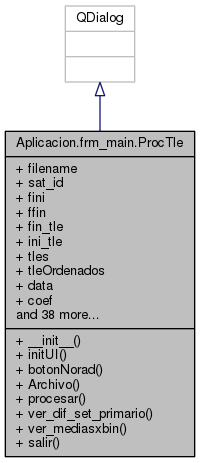
\includegraphics[width=222pt]{class_aplicacion_1_1frm__main_1_1_proc_tle__inherit__graph}
\end{center}
\end{figure}


\-Collaboration diagram for \-Aplicacion.\-frm\-\_\-main.\-Proc\-Tle\-:\nopagebreak
\begin{figure}[H]
\begin{center}
\leavevmode
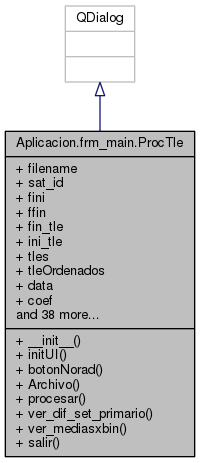
\includegraphics[width=222pt]{class_aplicacion_1_1frm__main_1_1_proc_tle__coll__graph}
\end{center}
\end{figure}
\subsection*{\-Public \-Member \-Functions}
\begin{DoxyCompactItemize}
\item 
def {\bf \-\_\-\-\_\-init\-\_\-\-\_\-}
\item 
def {\bf init\-U\-I}
\item 
def {\bf boton\-Norad}
\item 
def {\bf \-Archivo}
\item 
def {\bf procesar}
\item 
def {\bf ver\-\_\-dif\-\_\-set\-\_\-primario}
\item 
def {\bf ver\-\_\-mediasxbin}
\item 
def {\bf salir}
\end{DoxyCompactItemize}
\subsection*{\-Public \-Attributes}
\begin{DoxyCompactItemize}
\item 
{\bf filename}
\item 
{\bf sat\-\_\-id}
\item 
{\bf fini}
\item 
{\bf ffin}
\item 
{\bf fin\-\_\-tle}
\item 
{\bf ini\-\_\-tle}
\item 
{\bf tles}
\item 
{\bf tle\-Ordenados}
\item 
{\bf data}
\item 
{\bf coef}
\item 
{\bf path}
\item 
{\bf diferencias}
\item 
{\bf set\-\_\-data}
\item 
{\bf set\-\_\-pri}
\item 
{\bf arch\-\_\-macovar}
\item 
{\bf macovar\-T}
\item 
{\bf cantxbin}
\item 
{\bf mediaxbin}
\item 
{\bf palette}
\item 
{\bf carga}
\item 
{\bf norad}
\item 
{\bf equipo}
\item 
{\bf arch\-\_\-prepro}
\item 
{\bf sat\-\_\-id\-\_\-label}
\item 
{\bf cant\-\_\-tles}
\item 
{\bf tle\-\_\-pri}
\item 
{\bf outputs}
\item 
{\bf ma\-\_\-covar\-\_\-label}
\item 
{\bf boton\-\_\-norad}
\item 
{\bf boton\-\_\-equipo}
\item 
{\bf boton\-\_\-procesa}
\item 
{\bf boton\-\_\-dtotales}
\item 
{\bf boton\-\_\-dxcoord}
\item 
{\bf boton\-\_\-dsetprimario}
\item 
{\bf boton\-\_\-salir}
\item 
{\bf arch\-\_\-cargado}
\item 
{\bf sat\-\_\-id\-\_\-line}
\item 
{\bf cant\-\_\-tles\-\_\-edit}
\item 
{\bf matriz}
\item 
{\bf estado\-\_\-proc\-\_\-edit}
\item 
{\bf tle\-\_\-pri\-\_\-edit}
\item 
{\bf table\-View}
\item 
{\bf w}
\item 
{\bf lista}
\item 
{\bf tledic}
\item 
{\bf dt}
\item 
{\bf data1}
\item 
{\bf nombre\-\_\-archivo}
\end{DoxyCompactItemize}


\subsection{\-Detailed \-Description}


\-Definition at line 502 of file frm\-\_\-main.\-py.



\subsection{\-Constructor \& \-Destructor \-Documentation}
\index{\-Aplicacion\-::frm\-\_\-main\-::\-Proc\-Tle@{\-Aplicacion\-::frm\-\_\-main\-::\-Proc\-Tle}!\-\_\-\-\_\-init\-\_\-\-\_\-@{\-\_\-\-\_\-init\-\_\-\-\_\-}}
\index{\-\_\-\-\_\-init\-\_\-\-\_\-@{\-\_\-\-\_\-init\-\_\-\-\_\-}!Aplicacion::frm_main::ProcTle@{\-Aplicacion\-::frm\-\_\-main\-::\-Proc\-Tle}}
\subsubsection[{\-\_\-\-\_\-init\-\_\-\-\_\-}]{\setlength{\rightskip}{0pt plus 5cm}def {\bf \-Aplicacion.\-frm\-\_\-main.\-Proc\-Tle.\-\_\-\-\_\-init\-\_\-\-\_\-} (
\begin{DoxyParamCaption}
\item[{}]{self, }
\item[{}]{parent = {\ttfamily \-None}}
\end{DoxyParamCaption}
)}\label{class_aplicacion_1_1frm__main_1_1_proc_tle_a8a14007499f5229334b72bc388db6428}


\-Definition at line 504 of file frm\-\_\-main.\-py.


\begin{DoxyCode}
504 
505     def __init__(self,parent=None):
506         QDialog.__init__(self,parent)
507 
508         self.setWindowModality(Qt.ApplicationModal)
509         self.initUI()
510 
511         self.filename = ''
512         self.sat_id='99999'
513         self.fini=''
514         self.ffin=''
515         self.fin_tle=datetime(1957,1,1,0,0,0)
516         self.ini_tle=datetime(1957,1,1,0,0,0)
517         self.tles=0
518         self.tleOrdenados={}
519         self.data=[]
520         self.coef=[]
521         self.path='../AjustarTLE/diferencias/'
522         self.diferencias=''
523         self.set_data=[]
524         self.set_pri=[]
525         self.arch_macovar=''
526         self.macovarT=''  
527         self.cantxbin=[]
528         self.mediaxbin=[]      
        
\end{DoxyCode}


\subsection{\-Member \-Function \-Documentation}
\index{\-Aplicacion\-::frm\-\_\-main\-::\-Proc\-Tle@{\-Aplicacion\-::frm\-\_\-main\-::\-Proc\-Tle}!\-Archivo@{\-Archivo}}
\index{\-Archivo@{\-Archivo}!Aplicacion::frm_main::ProcTle@{\-Aplicacion\-::frm\-\_\-main\-::\-Proc\-Tle}}
\subsubsection[{\-Archivo}]{\setlength{\rightskip}{0pt plus 5cm}def {\bf \-Aplicacion.\-frm\-\_\-main.\-Proc\-Tle.\-Archivo} (
\begin{DoxyParamCaption}
\item[{}]{self}
\end{DoxyParamCaption}
)}\label{class_aplicacion_1_1frm__main_1_1_proc_tle_a9fc52e9ad9e366a48c39de5b0904140a}


\-Definition at line 622 of file frm\-\_\-main.\-py.


\begin{DoxyCode}
622 
623     def Archivo(self):    
624         fname=QFileDialog.getOpenFileName(self, 'Seleccione el Archivo a
       Procesar', "../TleAdmin/crudosTLE/*")
625         nombre=str(fname).split('/')[-1]
626         self.filename = nombre
627         self.sat_id = nombre.split('_')[0]
628         self.arch_cargado.setText(self.filename)
629         self.boton_procesa.setEnabled(True)
630         
    
\end{DoxyCode}
\index{\-Aplicacion\-::frm\-\_\-main\-::\-Proc\-Tle@{\-Aplicacion\-::frm\-\_\-main\-::\-Proc\-Tle}!boton\-Norad@{boton\-Norad}}
\index{boton\-Norad@{boton\-Norad}!Aplicacion::frm_main::ProcTle@{\-Aplicacion\-::frm\-\_\-main\-::\-Proc\-Tle}}
\subsubsection[{boton\-Norad}]{\setlength{\rightskip}{0pt plus 5cm}def {\bf \-Aplicacion.\-frm\-\_\-main.\-Proc\-Tle.\-boton\-Norad} (
\begin{DoxyParamCaption}
\item[{}]{self}
\end{DoxyParamCaption}
)}\label{class_aplicacion_1_1frm__main_1_1_proc_tle_a4c08618591a63dfe1eed6785d53b7877}


\-Definition at line 613 of file frm\-\_\-main.\-py.


\begin{DoxyCode}
613 
614     def botonNorad(self):
615         print ("Procesando la Conexion con NORAD para la Descarga...")
616         self.w = ConexionNorad()
617         self.w.exec_()
618         self.sat_id, self.fini, self.ffin, self.filename = 
      self.w.iniciaSolicitud()
619         self.arch_cargado.setText(self.filename)
620         self.sat_id_line.setText(self.sat_id) 
621         self.boton_procesa.setEnabled(True) 
        
\end{DoxyCode}
\index{\-Aplicacion\-::frm\-\_\-main\-::\-Proc\-Tle@{\-Aplicacion\-::frm\-\_\-main\-::\-Proc\-Tle}!init\-U\-I@{init\-U\-I}}
\index{init\-U\-I@{init\-U\-I}!Aplicacion::frm_main::ProcTle@{\-Aplicacion\-::frm\-\_\-main\-::\-Proc\-Tle}}
\subsubsection[{init\-U\-I}]{\setlength{\rightskip}{0pt plus 5cm}def {\bf \-Aplicacion.\-frm\-\_\-main.\-Proc\-Tle.\-init\-U\-I} (
\begin{DoxyParamCaption}
\item[{}]{self}
\end{DoxyParamCaption}
)}\label{class_aplicacion_1_1frm__main_1_1_proc_tle_aaf23e6957942a56690df1661246fe63a}


\-Definition at line 529 of file frm\-\_\-main.\-py.


\begin{DoxyCode}
529 
530     def initUI(self):
531         self.palette = QPalette()
532         self.palette.setColor(QPalette.Background,Qt.white)
533         self.setPalette(self.palette)
534         
535         """
536         Etiquetas
537         """
538         self.carga           = QLabel('CARGADO DE TLEs')
539         self.norad           = QLabel('A partir de NORAD')  
540         self.equipo          = QLabel('Desde el Equipo')
541         self.arch_prepro     = QLabel('Archivo a Procesar: ')
542         self.sat_id_label    = QLabel('NORAD_ID')
543         self.cant_tles       = QLabel('Cantidad de TLEs')
544         self.tle_pri         = QLabel('Ultimo TLE del set.')
545         self.outputs         = QLabel('Output')
546         self.ma_covar_label  = QLabel('Ma. de COVARIANZA')
547         """
548         Botones
549         """
550         self.boton_norad        = QPushButton('Space-Track')
551         self.boton_equipo       = QPushButton('Directorios')
552         self.boton_procesa      = QPushButton('PROCESAR')
553         self.boton_dtotales     = QPushButton('Graficar Diferencias Totales')
554         self.boton_dxcoord      = QPushButton('Graficar Diferencias por
       Coordenadas')
555         self.boton_dsetprimario = QPushButton ('Graficar Diferencias del Set
       primario')
556         self.boton_salir        = QPushButton('Salir')
557         """
558         Campos de Edicion
559         """
560         self.arch_cargado       = QLineEdit()
561         self.sat_id_line        = QLineEdit()
562         self.cant_tles_edit     = QLineEdit()
563         self.matriz             = QLineEdit()
564         self.estado_proc_edit   = QLineEdit()
565         """
566         OTROS
567         """
568         self.tle_pri_edit    = QTextEdit()
569         self.tableView       = QTableWidget()
570         """
571         Plantilla
572         """
573         grid = QGridLayout()
574         grid.setSpacing(5)
575         
576         grid.addWidget(self.carga,2,0)
577         grid.addWidget(self.norad,3,0)
578         grid.addWidget(self.boton_norad,3,1)
579         grid.addWidget(self.equipo,4,0)
580         grid.addWidget(self.boton_equipo,4,1)
581         grid.addWidget(self.arch_prepro,5,0)
582         grid.addWidget(self.arch_cargado,5,1)
583         grid.addWidget(self.boton_procesa,5,2)
584         grid.addWidget(self.sat_id_label,7,0)
585         grid.addWidget(self.sat_id_line,7,1)
586         grid.addWidget(self.cant_tles,8,0)
587         grid.addWidget(self.cant_tles_edit,8,1)        
588         grid.addWidget(self.tle_pri,9,0)
589         grid.addWidget(self.tle_pri_edit,10,0,1,4)
590         grid.addWidget(self.ma_covar_label,11,0) 
591         grid.addWidget(self.tableView,12,0)
592         grid.addWidget(self.outputs,23,1)
593         grid.addWidget(self.estado_proc_edit,23,2)
594         grid.addWidget(self.boton_dsetprimario,24,2)
595         grid.addWidget(self.boton_salir,25,2)
596 #         grid.addWidget(self.boton_dtotales,25,1)
597 #         grid.addWidget(self.boton_dxcoord,25,2)
598         
599         """
600         Acciones
601         """
602         self.boton_procesa.setEnabled(False)
603         self.boton_norad.clicked.connect(self.botonNorad)
604         self.boton_equipo.clicked.connect(self.Archivo)
605         self.boton_salir.clicked.connect(self.salir)
606         self.boton_procesa.clicked.connect(self.procesar)
607         self.boton_dsetprimario.clicked.connect(self.ver_dif_set_primario)
608 #         self.boton_dxcoord.clicked.connect(self.ver_dif_x_coordenadas)
609 #         self.boton_dtotales.clicked.connect(self.ver_diferencias_totales)
610         self.setLayout(grid)
611         self.setWindowTitle('Procesamiento de TLE')    
612         self.show()
          
\end{DoxyCode}
\index{\-Aplicacion\-::frm\-\_\-main\-::\-Proc\-Tle@{\-Aplicacion\-::frm\-\_\-main\-::\-Proc\-Tle}!procesar@{procesar}}
\index{procesar@{procesar}!Aplicacion::frm_main::ProcTle@{\-Aplicacion\-::frm\-\_\-main\-::\-Proc\-Tle}}
\subsubsection[{procesar}]{\setlength{\rightskip}{0pt plus 5cm}def {\bf \-Aplicacion.\-frm\-\_\-main.\-Proc\-Tle.\-procesar} (
\begin{DoxyParamCaption}
\item[{}]{self}
\end{DoxyParamCaption}
)}\label{class_aplicacion_1_1frm__main_1_1_proc_tle_a0efa8947e0fe54038f57f6aa46d39f44}
\begin{DoxyVerb}
Invoca a la funcion divide_setTLE, para fragmentar
cada uno de los TLE del dato crudo en archivos
individuales; y los guarda en: TleAdmin/tle
\end{DoxyVerb}
 

\-Definition at line 631 of file frm\-\_\-main.\-py.


\begin{DoxyCode}
631 
632     def procesar(self):
633         """
634         Invoca a la funcion divide_setTLE, para fragmentar
635         cada uno de los TLE del dato crudo en archivos
636         individuales; y los guarda en: TleAdmin/tle
637         """
638         files=glob.glob('../TleAdmin/tle/*')
639         for filename in files:
640             os.unlink(filename)
641         if os.stat('../TleAdmin/crudosTLE/'+self.filename).st_size == 0:
642             print('El archivo esta vacio')
643         divide_setTLE(self.sat_id, self.filename)
644         self.sat_id_line.setText(self.sat_id)
645         self.lista=glob.glob('../TleAdmin/tle/*')
646         self.tles=len(self.lista)
647         self.cant_tles_edit.setText(str(self.tles))
648         """
649         Ordenamiento de los TLEs
650         """
651         self.tledic=generadorDatos(self.lista)
652         self.tleOrdenados=ordenaTles(self.tledic)
653 
654         """
655         Impresiones de info de TLEs.
656         """
657         print 'PROCESAMIENTO DE TLE'
658         print '-----------------------------------------------------'
659         print 'TLE PRIMARIO'
660         print '-----------------------------------------------------'
661         tle_primario = Tle.creadoxArchivo('../TleAdmin/tle/'+self.tleOrdenados[
      -1][0])
662         linea1= tle_primario.linea1
663         linea2= tle_primario.linea2
664         self.fin_tle=tle_primario.epoca()
665         self.ffin=self.fin_tle.strftime('%Y-%m-%d %H:%M:%S.%f' )
666         self.tle_pri_edit.setText(linea1+'\n'+linea2)
667         print linea1
668         print linea2
669         print '-----------------------------------------------------'
670         print 'TLE INICIAL DEL SET'
671         print '-----------------------------------------------------'
672         tle_inial = Tle.creadoxArchivo('../TleAdmin/tle/'+self.tleOrdenados[0][
      0])
673         linea1_0= tle_inial.linea1
674         linea2_0= tle_inial.linea2
675         self.ini_tle=tle_inial.epoca()
676         print linea1_0
677         print linea2_0
678         print '-----------------------------------------------------'
679         
680         """
681         PROCESAMIENTO.
682         """
683         files=glob.glob('../AjustarTLE/diferencias/*')
684         for filename in files:
685             os.unlink(filename)
686 #        self.bin, self.data, self.set_pri, self.coef=difTle(self.tleOrdenados,
       self.tles)
687         self.set_pri=difPrimario()
688         self.dt=self.set_pri[0]
689         self.data1=self.set_pri[1]
690         self.coef=self.set_pri[2]
691         self.nombre_archivo=self.set_pri[3]
692 #         self.cantxbin,self.mediaxbin=genera_estadisticaBin(self.bin)
693 #         self.diferencias=difPrimario(self.nombre_archivo,self.tles-1)
694         self.estado_proc_edit.setText(self.nombre_archivo)
695 
696         """
697         Ma. de Covarianza
698         """
699         self.macovarT, self.arch_macovar=EjecutaMaCovar(self.nombre_archivo)
700         self.tableView.setRowCount(len(self.macovarT))
701         self.tableView.setColumnCount(len(self.macovarT))
702         for i,fila in enumerate(self.macovarT):
703             for j,col in enumerate(fila):
704                 self.tableView.setItem(i,j,QTableWidgetItem(str(col)))    
705         
706         print 'Fin del Procesamiento'
707         
708 #     def ver_dif_x_coordenadas(self):
709 #         ploteos.grafica_setcompleto(self.sat_id,self.path,self.data1,
       self.coef)
710 #      
711 #     def ver_diferencias_totales(self):
712 #        
       ploteos.grafica_diferenciasTotales(self.sat_id,self.path,self.data1,self.coef) 
        
\end{DoxyCode}
\index{\-Aplicacion\-::frm\-\_\-main\-::\-Proc\-Tle@{\-Aplicacion\-::frm\-\_\-main\-::\-Proc\-Tle}!salir@{salir}}
\index{salir@{salir}!Aplicacion::frm_main::ProcTle@{\-Aplicacion\-::frm\-\_\-main\-::\-Proc\-Tle}}
\subsubsection[{salir}]{\setlength{\rightskip}{0pt plus 5cm}def {\bf \-Aplicacion.\-frm\-\_\-main.\-Proc\-Tle.\-salir} (
\begin{DoxyParamCaption}
\item[{}]{self}
\end{DoxyParamCaption}
)}\label{class_aplicacion_1_1frm__main_1_1_proc_tle_a83cf8f64ae3064bb6ef4923a244ca807}


\-Definition at line 734 of file frm\-\_\-main.\-py.


\begin{DoxyCode}
734 
735     def salir(self):
736         self.accept()

\end{DoxyCode}
\index{\-Aplicacion\-::frm\-\_\-main\-::\-Proc\-Tle@{\-Aplicacion\-::frm\-\_\-main\-::\-Proc\-Tle}!ver\-\_\-dif\-\_\-set\-\_\-primario@{ver\-\_\-dif\-\_\-set\-\_\-primario}}
\index{ver\-\_\-dif\-\_\-set\-\_\-primario@{ver\-\_\-dif\-\_\-set\-\_\-primario}!Aplicacion::frm_main::ProcTle@{\-Aplicacion\-::frm\-\_\-main\-::\-Proc\-Tle}}
\subsubsection[{ver\-\_\-dif\-\_\-set\-\_\-primario}]{\setlength{\rightskip}{0pt plus 5cm}def {\bf \-Aplicacion.\-frm\-\_\-main.\-Proc\-Tle.\-ver\-\_\-dif\-\_\-set\-\_\-primario} (
\begin{DoxyParamCaption}
\item[{}]{self}
\end{DoxyParamCaption}
)}\label{class_aplicacion_1_1frm__main_1_1_proc_tle_a9b7bf8fdffe010b12798bbd6b98578b5}


\-Definition at line 713 of file frm\-\_\-main.\-py.


\begin{DoxyCode}
713 
714     def ver_dif_set_primario(self):
715         ploteos.grafica_set_principal(self.sat_id,self.path, self.data1,self.
      coef)
716         
717 #     def Graficar(self):
718 # #        data=[self.sat_id,self.diferencias,self.cantxbin, self.mediaxbin]
719 #         data=[self.sat_id,self.diferencias]
720 #         self.graf = RepresentacionGrafica(data)
721 #         self.graf.exec_()
        
\end{DoxyCode}
\index{\-Aplicacion\-::frm\-\_\-main\-::\-Proc\-Tle@{\-Aplicacion\-::frm\-\_\-main\-::\-Proc\-Tle}!ver\-\_\-mediasxbin@{ver\-\_\-mediasxbin}}
\index{ver\-\_\-mediasxbin@{ver\-\_\-mediasxbin}!Aplicacion::frm_main::ProcTle@{\-Aplicacion\-::frm\-\_\-main\-::\-Proc\-Tle}}
\subsubsection[{ver\-\_\-mediasxbin}]{\setlength{\rightskip}{0pt plus 5cm}def {\bf \-Aplicacion.\-frm\-\_\-main.\-Proc\-Tle.\-ver\-\_\-mediasxbin} (
\begin{DoxyParamCaption}
\item[{}]{self}
\end{DoxyParamCaption}
)}\label{class_aplicacion_1_1frm__main_1_1_proc_tle_a1e55b3bd59f3d4eb73585631bf02f225}


\-Definition at line 722 of file frm\-\_\-main.\-py.


\begin{DoxyCode}
722 
723     def ver_mediasxbin(self):
724         desviacion_standard_graf(self.sat_id, self.mediaxbin[0], self.mediaxbin
      [1], self.mediaxbin[2])
725 
726 #     def Macovar(self):
727 #         self.macovarT, self.arch_macovar=EjecutaMaCovar(self.diferencias)
728 #         self.tableView.setRowCount(len(self.macovarT))
729 #         self.tableView.setColumnCount(len(self.macovarT))
730 #         for i,fila in enumerate(self.macovarT):
731 #             for j,col in enumerate(fila):
732 #                 self.tableView.setItem(i,j,QTableWidgetItem(str(col)))
733 #         self.arch_macovar_edit.setText(self.arch_macovar)        
    
\end{DoxyCode}


\-Here is the call graph for this function\-:\nopagebreak
\begin{figure}[H]
\begin{center}
\leavevmode
\includegraphics[width=350pt]{class_aplicacion_1_1frm__main_1_1_proc_tle_a1e55b3bd59f3d4eb73585631bf02f225_cgraph}
\end{center}
\end{figure}




\subsection{\-Member \-Data \-Documentation}
\index{\-Aplicacion\-::frm\-\_\-main\-::\-Proc\-Tle@{\-Aplicacion\-::frm\-\_\-main\-::\-Proc\-Tle}!arch\-\_\-cargado@{arch\-\_\-cargado}}
\index{arch\-\_\-cargado@{arch\-\_\-cargado}!Aplicacion::frm_main::ProcTle@{\-Aplicacion\-::frm\-\_\-main\-::\-Proc\-Tle}}
\subsubsection[{arch\-\_\-cargado}]{\setlength{\rightskip}{0pt plus 5cm}{\bf \-Aplicacion\-::frm\-\_\-main.\-Proc\-Tle\-::arch\-\_\-cargado}}\label{class_aplicacion_1_1frm__main_1_1_proc_tle_a8d25d88316b65c3168f35a121c50e387}


\-Definition at line 535 of file frm\-\_\-main.\-py.

\index{\-Aplicacion\-::frm\-\_\-main\-::\-Proc\-Tle@{\-Aplicacion\-::frm\-\_\-main\-::\-Proc\-Tle}!arch\-\_\-macovar@{arch\-\_\-macovar}}
\index{arch\-\_\-macovar@{arch\-\_\-macovar}!Aplicacion::frm_main::ProcTle@{\-Aplicacion\-::frm\-\_\-main\-::\-Proc\-Tle}}
\subsubsection[{arch\-\_\-macovar}]{\setlength{\rightskip}{0pt plus 5cm}{\bf \-Aplicacion\-::frm\-\_\-main.\-Proc\-Tle\-::arch\-\_\-macovar}}\label{class_aplicacion_1_1frm__main_1_1_proc_tle_a1ccdf851f71df42b3825b20eee64e92f}


\-Definition at line 504 of file frm\-\_\-main.\-py.

\index{\-Aplicacion\-::frm\-\_\-main\-::\-Proc\-Tle@{\-Aplicacion\-::frm\-\_\-main\-::\-Proc\-Tle}!arch\-\_\-prepro@{arch\-\_\-prepro}}
\index{arch\-\_\-prepro@{arch\-\_\-prepro}!Aplicacion::frm_main::ProcTle@{\-Aplicacion\-::frm\-\_\-main\-::\-Proc\-Tle}}
\subsubsection[{arch\-\_\-prepro}]{\setlength{\rightskip}{0pt plus 5cm}{\bf \-Aplicacion\-::frm\-\_\-main.\-Proc\-Tle\-::arch\-\_\-prepro}}\label{class_aplicacion_1_1frm__main_1_1_proc_tle_ad43d79e0743fc7352335d7f001d081c5}


\-Definition at line 531 of file frm\-\_\-main.\-py.

\index{\-Aplicacion\-::frm\-\_\-main\-::\-Proc\-Tle@{\-Aplicacion\-::frm\-\_\-main\-::\-Proc\-Tle}!boton\-\_\-dsetprimario@{boton\-\_\-dsetprimario}}
\index{boton\-\_\-dsetprimario@{boton\-\_\-dsetprimario}!Aplicacion::frm_main::ProcTle@{\-Aplicacion\-::frm\-\_\-main\-::\-Proc\-Tle}}
\subsubsection[{boton\-\_\-dsetprimario}]{\setlength{\rightskip}{0pt plus 5cm}{\bf \-Aplicacion\-::frm\-\_\-main.\-Proc\-Tle\-::boton\-\_\-dsetprimario}}\label{class_aplicacion_1_1frm__main_1_1_proc_tle_a7631d0d1e7c28883fb96234ce67e7492}


\-Definition at line 533 of file frm\-\_\-main.\-py.

\index{\-Aplicacion\-::frm\-\_\-main\-::\-Proc\-Tle@{\-Aplicacion\-::frm\-\_\-main\-::\-Proc\-Tle}!boton\-\_\-dtotales@{boton\-\_\-dtotales}}
\index{boton\-\_\-dtotales@{boton\-\_\-dtotales}!Aplicacion::frm_main::ProcTle@{\-Aplicacion\-::frm\-\_\-main\-::\-Proc\-Tle}}
\subsubsection[{boton\-\_\-dtotales}]{\setlength{\rightskip}{0pt plus 5cm}{\bf \-Aplicacion\-::frm\-\_\-main.\-Proc\-Tle\-::boton\-\_\-dtotales}}\label{class_aplicacion_1_1frm__main_1_1_proc_tle_a15f64c9f5fb87cb7c8e2c0b20f605501}


\-Definition at line 533 of file frm\-\_\-main.\-py.

\index{\-Aplicacion\-::frm\-\_\-main\-::\-Proc\-Tle@{\-Aplicacion\-::frm\-\_\-main\-::\-Proc\-Tle}!boton\-\_\-dxcoord@{boton\-\_\-dxcoord}}
\index{boton\-\_\-dxcoord@{boton\-\_\-dxcoord}!Aplicacion::frm_main::ProcTle@{\-Aplicacion\-::frm\-\_\-main\-::\-Proc\-Tle}}
\subsubsection[{boton\-\_\-dxcoord}]{\setlength{\rightskip}{0pt plus 5cm}{\bf \-Aplicacion\-::frm\-\_\-main.\-Proc\-Tle\-::boton\-\_\-dxcoord}}\label{class_aplicacion_1_1frm__main_1_1_proc_tle_a96a285eb182d86af4677ba5b57b1791f}


\-Definition at line 533 of file frm\-\_\-main.\-py.

\index{\-Aplicacion\-::frm\-\_\-main\-::\-Proc\-Tle@{\-Aplicacion\-::frm\-\_\-main\-::\-Proc\-Tle}!boton\-\_\-equipo@{boton\-\_\-equipo}}
\index{boton\-\_\-equipo@{boton\-\_\-equipo}!Aplicacion::frm_main::ProcTle@{\-Aplicacion\-::frm\-\_\-main\-::\-Proc\-Tle}}
\subsubsection[{boton\-\_\-equipo}]{\setlength{\rightskip}{0pt plus 5cm}{\bf \-Aplicacion\-::frm\-\_\-main.\-Proc\-Tle\-::boton\-\_\-equipo}}\label{class_aplicacion_1_1frm__main_1_1_proc_tle_a402cbf3922e656ca7b19069df0357dc2}


\-Definition at line 533 of file frm\-\_\-main.\-py.

\index{\-Aplicacion\-::frm\-\_\-main\-::\-Proc\-Tle@{\-Aplicacion\-::frm\-\_\-main\-::\-Proc\-Tle}!boton\-\_\-norad@{boton\-\_\-norad}}
\index{boton\-\_\-norad@{boton\-\_\-norad}!Aplicacion::frm_main::ProcTle@{\-Aplicacion\-::frm\-\_\-main\-::\-Proc\-Tle}}
\subsubsection[{boton\-\_\-norad}]{\setlength{\rightskip}{0pt plus 5cm}{\bf \-Aplicacion\-::frm\-\_\-main.\-Proc\-Tle\-::boton\-\_\-norad}}\label{class_aplicacion_1_1frm__main_1_1_proc_tle_a6994359117a8a6ebd6b127a5fbb4ea94}


\-Definition at line 533 of file frm\-\_\-main.\-py.

\index{\-Aplicacion\-::frm\-\_\-main\-::\-Proc\-Tle@{\-Aplicacion\-::frm\-\_\-main\-::\-Proc\-Tle}!boton\-\_\-procesa@{boton\-\_\-procesa}}
\index{boton\-\_\-procesa@{boton\-\_\-procesa}!Aplicacion::frm_main::ProcTle@{\-Aplicacion\-::frm\-\_\-main\-::\-Proc\-Tle}}
\subsubsection[{boton\-\_\-procesa}]{\setlength{\rightskip}{0pt plus 5cm}{\bf \-Aplicacion\-::frm\-\_\-main.\-Proc\-Tle\-::boton\-\_\-procesa}}\label{class_aplicacion_1_1frm__main_1_1_proc_tle_a5f38e23fd65221917002fcf892340ae4}


\-Definition at line 533 of file frm\-\_\-main.\-py.

\index{\-Aplicacion\-::frm\-\_\-main\-::\-Proc\-Tle@{\-Aplicacion\-::frm\-\_\-main\-::\-Proc\-Tle}!boton\-\_\-salir@{boton\-\_\-salir}}
\index{boton\-\_\-salir@{boton\-\_\-salir}!Aplicacion::frm_main::ProcTle@{\-Aplicacion\-::frm\-\_\-main\-::\-Proc\-Tle}}
\subsubsection[{boton\-\_\-salir}]{\setlength{\rightskip}{0pt plus 5cm}{\bf \-Aplicacion\-::frm\-\_\-main.\-Proc\-Tle\-::boton\-\_\-salir}}\label{class_aplicacion_1_1frm__main_1_1_proc_tle_a53caa6ae5f98ae241b26229db6ce5bd7}


\-Definition at line 533 of file frm\-\_\-main.\-py.

\index{\-Aplicacion\-::frm\-\_\-main\-::\-Proc\-Tle@{\-Aplicacion\-::frm\-\_\-main\-::\-Proc\-Tle}!cant\-\_\-tles@{cant\-\_\-tles}}
\index{cant\-\_\-tles@{cant\-\_\-tles}!Aplicacion::frm_main::ProcTle@{\-Aplicacion\-::frm\-\_\-main\-::\-Proc\-Tle}}
\subsubsection[{cant\-\_\-tles}]{\setlength{\rightskip}{0pt plus 5cm}{\bf \-Aplicacion\-::frm\-\_\-main.\-Proc\-Tle\-::cant\-\_\-tles}}\label{class_aplicacion_1_1frm__main_1_1_proc_tle_ac20e8aaa26b77b63146bb4b075371f5f}


\-Definition at line 531 of file frm\-\_\-main.\-py.

\index{\-Aplicacion\-::frm\-\_\-main\-::\-Proc\-Tle@{\-Aplicacion\-::frm\-\_\-main\-::\-Proc\-Tle}!cant\-\_\-tles\-\_\-edit@{cant\-\_\-tles\-\_\-edit}}
\index{cant\-\_\-tles\-\_\-edit@{cant\-\_\-tles\-\_\-edit}!Aplicacion::frm_main::ProcTle@{\-Aplicacion\-::frm\-\_\-main\-::\-Proc\-Tle}}
\subsubsection[{cant\-\_\-tles\-\_\-edit}]{\setlength{\rightskip}{0pt plus 5cm}{\bf \-Aplicacion\-::frm\-\_\-main.\-Proc\-Tle\-::cant\-\_\-tles\-\_\-edit}}\label{class_aplicacion_1_1frm__main_1_1_proc_tle_aabcccf0dd24ae037d0fd45095dbb7e4b}


\-Definition at line 535 of file frm\-\_\-main.\-py.

\index{\-Aplicacion\-::frm\-\_\-main\-::\-Proc\-Tle@{\-Aplicacion\-::frm\-\_\-main\-::\-Proc\-Tle}!cantxbin@{cantxbin}}
\index{cantxbin@{cantxbin}!Aplicacion::frm_main::ProcTle@{\-Aplicacion\-::frm\-\_\-main\-::\-Proc\-Tle}}
\subsubsection[{cantxbin}]{\setlength{\rightskip}{0pt plus 5cm}{\bf \-Aplicacion\-::frm\-\_\-main.\-Proc\-Tle\-::cantxbin}}\label{class_aplicacion_1_1frm__main_1_1_proc_tle_a9829a722583b1f1faeb4f260e4a935fa}


\-Definition at line 504 of file frm\-\_\-main.\-py.

\index{\-Aplicacion\-::frm\-\_\-main\-::\-Proc\-Tle@{\-Aplicacion\-::frm\-\_\-main\-::\-Proc\-Tle}!carga@{carga}}
\index{carga@{carga}!Aplicacion::frm_main::ProcTle@{\-Aplicacion\-::frm\-\_\-main\-::\-Proc\-Tle}}
\subsubsection[{carga}]{\setlength{\rightskip}{0pt plus 5cm}{\bf \-Aplicacion\-::frm\-\_\-main.\-Proc\-Tle\-::carga}}\label{class_aplicacion_1_1frm__main_1_1_proc_tle_ad99c9a4d2e2355816b5a3362c385a140}


\-Definition at line 531 of file frm\-\_\-main.\-py.

\index{\-Aplicacion\-::frm\-\_\-main\-::\-Proc\-Tle@{\-Aplicacion\-::frm\-\_\-main\-::\-Proc\-Tle}!coef@{coef}}
\index{coef@{coef}!Aplicacion::frm_main::ProcTle@{\-Aplicacion\-::frm\-\_\-main\-::\-Proc\-Tle}}
\subsubsection[{coef}]{\setlength{\rightskip}{0pt plus 5cm}{\bf \-Aplicacion\-::frm\-\_\-main.\-Proc\-Tle\-::coef}}\label{class_aplicacion_1_1frm__main_1_1_proc_tle_ae18d2fd96fbf6088a5553e3f111fbbc1}


\-Definition at line 504 of file frm\-\_\-main.\-py.

\index{\-Aplicacion\-::frm\-\_\-main\-::\-Proc\-Tle@{\-Aplicacion\-::frm\-\_\-main\-::\-Proc\-Tle}!data@{data}}
\index{data@{data}!Aplicacion::frm_main::ProcTle@{\-Aplicacion\-::frm\-\_\-main\-::\-Proc\-Tle}}
\subsubsection[{data}]{\setlength{\rightskip}{0pt plus 5cm}{\bf \-Aplicacion\-::frm\-\_\-main.\-Proc\-Tle\-::data}}\label{class_aplicacion_1_1frm__main_1_1_proc_tle_a8737c8fdf74468b499a0b9ef521fdb0c}


\-Definition at line 504 of file frm\-\_\-main.\-py.

\index{\-Aplicacion\-::frm\-\_\-main\-::\-Proc\-Tle@{\-Aplicacion\-::frm\-\_\-main\-::\-Proc\-Tle}!data1@{data1}}
\index{data1@{data1}!Aplicacion::frm_main::ProcTle@{\-Aplicacion\-::frm\-\_\-main\-::\-Proc\-Tle}}
\subsubsection[{data1}]{\setlength{\rightskip}{0pt plus 5cm}{\bf \-Aplicacion\-::frm\-\_\-main.\-Proc\-Tle\-::data1}}\label{class_aplicacion_1_1frm__main_1_1_proc_tle_a7979e3941bd5f486fa3d9a7b03d01629}


\-Definition at line 641 of file frm\-\_\-main.\-py.

\index{\-Aplicacion\-::frm\-\_\-main\-::\-Proc\-Tle@{\-Aplicacion\-::frm\-\_\-main\-::\-Proc\-Tle}!diferencias@{diferencias}}
\index{diferencias@{diferencias}!Aplicacion::frm_main::ProcTle@{\-Aplicacion\-::frm\-\_\-main\-::\-Proc\-Tle}}
\subsubsection[{diferencias}]{\setlength{\rightskip}{0pt plus 5cm}{\bf \-Aplicacion\-::frm\-\_\-main.\-Proc\-Tle\-::diferencias}}\label{class_aplicacion_1_1frm__main_1_1_proc_tle_a413cc4964b14c7f9d9ef98b11b68073b}


\-Definition at line 504 of file frm\-\_\-main.\-py.

\index{\-Aplicacion\-::frm\-\_\-main\-::\-Proc\-Tle@{\-Aplicacion\-::frm\-\_\-main\-::\-Proc\-Tle}!dt@{dt}}
\index{dt@{dt}!Aplicacion::frm_main::ProcTle@{\-Aplicacion\-::frm\-\_\-main\-::\-Proc\-Tle}}
\subsubsection[{dt}]{\setlength{\rightskip}{0pt plus 5cm}{\bf \-Aplicacion\-::frm\-\_\-main.\-Proc\-Tle\-::dt}}\label{class_aplicacion_1_1frm__main_1_1_proc_tle_af0f8f9c39379ee193e098aeaf58487c1}


\-Definition at line 641 of file frm\-\_\-main.\-py.

\index{\-Aplicacion\-::frm\-\_\-main\-::\-Proc\-Tle@{\-Aplicacion\-::frm\-\_\-main\-::\-Proc\-Tle}!equipo@{equipo}}
\index{equipo@{equipo}!Aplicacion::frm_main::ProcTle@{\-Aplicacion\-::frm\-\_\-main\-::\-Proc\-Tle}}
\subsubsection[{equipo}]{\setlength{\rightskip}{0pt plus 5cm}{\bf \-Aplicacion\-::frm\-\_\-main.\-Proc\-Tle\-::equipo}}\label{class_aplicacion_1_1frm__main_1_1_proc_tle_ae5a7fa4b802defc3a390262b5f8de1c7}


\-Definition at line 531 of file frm\-\_\-main.\-py.

\index{\-Aplicacion\-::frm\-\_\-main\-::\-Proc\-Tle@{\-Aplicacion\-::frm\-\_\-main\-::\-Proc\-Tle}!estado\-\_\-proc\-\_\-edit@{estado\-\_\-proc\-\_\-edit}}
\index{estado\-\_\-proc\-\_\-edit@{estado\-\_\-proc\-\_\-edit}!Aplicacion::frm_main::ProcTle@{\-Aplicacion\-::frm\-\_\-main\-::\-Proc\-Tle}}
\subsubsection[{estado\-\_\-proc\-\_\-edit}]{\setlength{\rightskip}{0pt plus 5cm}{\bf \-Aplicacion\-::frm\-\_\-main.\-Proc\-Tle\-::estado\-\_\-proc\-\_\-edit}}\label{class_aplicacion_1_1frm__main_1_1_proc_tle_ad7f43026c3d60ca9327e1c85c0ea5087}


\-Definition at line 535 of file frm\-\_\-main.\-py.

\index{\-Aplicacion\-::frm\-\_\-main\-::\-Proc\-Tle@{\-Aplicacion\-::frm\-\_\-main\-::\-Proc\-Tle}!ffin@{ffin}}
\index{ffin@{ffin}!Aplicacion::frm_main::ProcTle@{\-Aplicacion\-::frm\-\_\-main\-::\-Proc\-Tle}}
\subsubsection[{ffin}]{\setlength{\rightskip}{0pt plus 5cm}{\bf \-Aplicacion\-::frm\-\_\-main.\-Proc\-Tle\-::ffin}}\label{class_aplicacion_1_1frm__main_1_1_proc_tle_a58e224fd1d6ba81c336e3bdfa389a174}


\-Definition at line 504 of file frm\-\_\-main.\-py.

\index{\-Aplicacion\-::frm\-\_\-main\-::\-Proc\-Tle@{\-Aplicacion\-::frm\-\_\-main\-::\-Proc\-Tle}!filename@{filename}}
\index{filename@{filename}!Aplicacion::frm_main::ProcTle@{\-Aplicacion\-::frm\-\_\-main\-::\-Proc\-Tle}}
\subsubsection[{filename}]{\setlength{\rightskip}{0pt plus 5cm}{\bf \-Aplicacion\-::frm\-\_\-main.\-Proc\-Tle\-::filename}}\label{class_aplicacion_1_1frm__main_1_1_proc_tle_a3337b73115f16528a50aa5d2b959d17c}


\-Definition at line 504 of file frm\-\_\-main.\-py.

\index{\-Aplicacion\-::frm\-\_\-main\-::\-Proc\-Tle@{\-Aplicacion\-::frm\-\_\-main\-::\-Proc\-Tle}!fin\-\_\-tle@{fin\-\_\-tle}}
\index{fin\-\_\-tle@{fin\-\_\-tle}!Aplicacion::frm_main::ProcTle@{\-Aplicacion\-::frm\-\_\-main\-::\-Proc\-Tle}}
\subsubsection[{fin\-\_\-tle}]{\setlength{\rightskip}{0pt plus 5cm}{\bf \-Aplicacion\-::frm\-\_\-main.\-Proc\-Tle\-::fin\-\_\-tle}}\label{class_aplicacion_1_1frm__main_1_1_proc_tle_a7de8fb374fc149ea98078a4217206b3f}


\-Definition at line 504 of file frm\-\_\-main.\-py.

\index{\-Aplicacion\-::frm\-\_\-main\-::\-Proc\-Tle@{\-Aplicacion\-::frm\-\_\-main\-::\-Proc\-Tle}!fini@{fini}}
\index{fini@{fini}!Aplicacion::frm_main::ProcTle@{\-Aplicacion\-::frm\-\_\-main\-::\-Proc\-Tle}}
\subsubsection[{fini}]{\setlength{\rightskip}{0pt plus 5cm}{\bf \-Aplicacion\-::frm\-\_\-main.\-Proc\-Tle\-::fini}}\label{class_aplicacion_1_1frm__main_1_1_proc_tle_a59873ea4b0ed0285d60ea4df68cdfacf}


\-Definition at line 504 of file frm\-\_\-main.\-py.

\index{\-Aplicacion\-::frm\-\_\-main\-::\-Proc\-Tle@{\-Aplicacion\-::frm\-\_\-main\-::\-Proc\-Tle}!ini\-\_\-tle@{ini\-\_\-tle}}
\index{ini\-\_\-tle@{ini\-\_\-tle}!Aplicacion::frm_main::ProcTle@{\-Aplicacion\-::frm\-\_\-main\-::\-Proc\-Tle}}
\subsubsection[{ini\-\_\-tle}]{\setlength{\rightskip}{0pt plus 5cm}{\bf \-Aplicacion\-::frm\-\_\-main.\-Proc\-Tle\-::ini\-\_\-tle}}\label{class_aplicacion_1_1frm__main_1_1_proc_tle_a7df4e51f089cfdef54208e9665befc93}


\-Definition at line 504 of file frm\-\_\-main.\-py.

\index{\-Aplicacion\-::frm\-\_\-main\-::\-Proc\-Tle@{\-Aplicacion\-::frm\-\_\-main\-::\-Proc\-Tle}!lista@{lista}}
\index{lista@{lista}!Aplicacion::frm_main::ProcTle@{\-Aplicacion\-::frm\-\_\-main\-::\-Proc\-Tle}}
\subsubsection[{lista}]{\setlength{\rightskip}{0pt plus 5cm}{\bf \-Aplicacion\-::frm\-\_\-main.\-Proc\-Tle\-::lista}}\label{class_aplicacion_1_1frm__main_1_1_proc_tle_a19ebac4a83060f49ae0bb675e61917ad}


\-Definition at line 635 of file frm\-\_\-main.\-py.

\index{\-Aplicacion\-::frm\-\_\-main\-::\-Proc\-Tle@{\-Aplicacion\-::frm\-\_\-main\-::\-Proc\-Tle}!ma\-\_\-covar\-\_\-label@{ma\-\_\-covar\-\_\-label}}
\index{ma\-\_\-covar\-\_\-label@{ma\-\_\-covar\-\_\-label}!Aplicacion::frm_main::ProcTle@{\-Aplicacion\-::frm\-\_\-main\-::\-Proc\-Tle}}
\subsubsection[{ma\-\_\-covar\-\_\-label}]{\setlength{\rightskip}{0pt plus 5cm}{\bf \-Aplicacion\-::frm\-\_\-main.\-Proc\-Tle\-::ma\-\_\-covar\-\_\-label}}\label{class_aplicacion_1_1frm__main_1_1_proc_tle_a5521eb511dd0d0422d35827a63aa7259}


\-Definition at line 531 of file frm\-\_\-main.\-py.

\index{\-Aplicacion\-::frm\-\_\-main\-::\-Proc\-Tle@{\-Aplicacion\-::frm\-\_\-main\-::\-Proc\-Tle}!macovar\-T@{macovar\-T}}
\index{macovar\-T@{macovar\-T}!Aplicacion::frm_main::ProcTle@{\-Aplicacion\-::frm\-\_\-main\-::\-Proc\-Tle}}
\subsubsection[{macovar\-T}]{\setlength{\rightskip}{0pt plus 5cm}{\bf \-Aplicacion\-::frm\-\_\-main.\-Proc\-Tle\-::macovar\-T}}\label{class_aplicacion_1_1frm__main_1_1_proc_tle_a718c19c132988b408b03ae60f91986ea}


\-Definition at line 504 of file frm\-\_\-main.\-py.

\index{\-Aplicacion\-::frm\-\_\-main\-::\-Proc\-Tle@{\-Aplicacion\-::frm\-\_\-main\-::\-Proc\-Tle}!matriz@{matriz}}
\index{matriz@{matriz}!Aplicacion::frm_main::ProcTle@{\-Aplicacion\-::frm\-\_\-main\-::\-Proc\-Tle}}
\subsubsection[{matriz}]{\setlength{\rightskip}{0pt plus 5cm}{\bf \-Aplicacion\-::frm\-\_\-main.\-Proc\-Tle\-::matriz}}\label{class_aplicacion_1_1frm__main_1_1_proc_tle_a7437101e793904703cc0856ec1bf180d}


\-Definition at line 535 of file frm\-\_\-main.\-py.

\index{\-Aplicacion\-::frm\-\_\-main\-::\-Proc\-Tle@{\-Aplicacion\-::frm\-\_\-main\-::\-Proc\-Tle}!mediaxbin@{mediaxbin}}
\index{mediaxbin@{mediaxbin}!Aplicacion::frm_main::ProcTle@{\-Aplicacion\-::frm\-\_\-main\-::\-Proc\-Tle}}
\subsubsection[{mediaxbin}]{\setlength{\rightskip}{0pt plus 5cm}{\bf \-Aplicacion\-::frm\-\_\-main.\-Proc\-Tle\-::mediaxbin}}\label{class_aplicacion_1_1frm__main_1_1_proc_tle_a56c19935024758aa57df46f3ae01d558}


\-Definition at line 504 of file frm\-\_\-main.\-py.

\index{\-Aplicacion\-::frm\-\_\-main\-::\-Proc\-Tle@{\-Aplicacion\-::frm\-\_\-main\-::\-Proc\-Tle}!nombre\-\_\-archivo@{nombre\-\_\-archivo}}
\index{nombre\-\_\-archivo@{nombre\-\_\-archivo}!Aplicacion::frm_main::ProcTle@{\-Aplicacion\-::frm\-\_\-main\-::\-Proc\-Tle}}
\subsubsection[{nombre\-\_\-archivo}]{\setlength{\rightskip}{0pt plus 5cm}{\bf \-Aplicacion\-::frm\-\_\-main.\-Proc\-Tle\-::nombre\-\_\-archivo}}\label{class_aplicacion_1_1frm__main_1_1_proc_tle_a5f33a0440e48211cf4a46e28db154959}


\-Definition at line 641 of file frm\-\_\-main.\-py.

\index{\-Aplicacion\-::frm\-\_\-main\-::\-Proc\-Tle@{\-Aplicacion\-::frm\-\_\-main\-::\-Proc\-Tle}!norad@{norad}}
\index{norad@{norad}!Aplicacion::frm_main::ProcTle@{\-Aplicacion\-::frm\-\_\-main\-::\-Proc\-Tle}}
\subsubsection[{norad}]{\setlength{\rightskip}{0pt plus 5cm}{\bf \-Aplicacion\-::frm\-\_\-main.\-Proc\-Tle\-::norad}}\label{class_aplicacion_1_1frm__main_1_1_proc_tle_a1a0c1a134203bf3d395e386a784862d5}


\-Definition at line 531 of file frm\-\_\-main.\-py.

\index{\-Aplicacion\-::frm\-\_\-main\-::\-Proc\-Tle@{\-Aplicacion\-::frm\-\_\-main\-::\-Proc\-Tle}!outputs@{outputs}}
\index{outputs@{outputs}!Aplicacion::frm_main::ProcTle@{\-Aplicacion\-::frm\-\_\-main\-::\-Proc\-Tle}}
\subsubsection[{outputs}]{\setlength{\rightskip}{0pt plus 5cm}{\bf \-Aplicacion\-::frm\-\_\-main.\-Proc\-Tle\-::outputs}}\label{class_aplicacion_1_1frm__main_1_1_proc_tle_afc1e344f9f10e9b9d2fd2f0b4a3d0531}


\-Definition at line 531 of file frm\-\_\-main.\-py.

\index{\-Aplicacion\-::frm\-\_\-main\-::\-Proc\-Tle@{\-Aplicacion\-::frm\-\_\-main\-::\-Proc\-Tle}!palette@{palette}}
\index{palette@{palette}!Aplicacion::frm_main::ProcTle@{\-Aplicacion\-::frm\-\_\-main\-::\-Proc\-Tle}}
\subsubsection[{palette}]{\setlength{\rightskip}{0pt plus 5cm}{\bf \-Aplicacion\-::frm\-\_\-main.\-Proc\-Tle\-::palette}}\label{class_aplicacion_1_1frm__main_1_1_proc_tle_ae191ee397d01d8050eeb7ee0b1968c31}


\-Definition at line 529 of file frm\-\_\-main.\-py.

\index{\-Aplicacion\-::frm\-\_\-main\-::\-Proc\-Tle@{\-Aplicacion\-::frm\-\_\-main\-::\-Proc\-Tle}!path@{path}}
\index{path@{path}!Aplicacion::frm_main::ProcTle@{\-Aplicacion\-::frm\-\_\-main\-::\-Proc\-Tle}}
\subsubsection[{path}]{\setlength{\rightskip}{0pt plus 5cm}{\bf \-Aplicacion\-::frm\-\_\-main.\-Proc\-Tle\-::path}}\label{class_aplicacion_1_1frm__main_1_1_proc_tle_a6309e51089a511eb2d243cc9e1e2f6e0}


\-Definition at line 504 of file frm\-\_\-main.\-py.

\index{\-Aplicacion\-::frm\-\_\-main\-::\-Proc\-Tle@{\-Aplicacion\-::frm\-\_\-main\-::\-Proc\-Tle}!sat\-\_\-id@{sat\-\_\-id}}
\index{sat\-\_\-id@{sat\-\_\-id}!Aplicacion::frm_main::ProcTle@{\-Aplicacion\-::frm\-\_\-main\-::\-Proc\-Tle}}
\subsubsection[{sat\-\_\-id}]{\setlength{\rightskip}{0pt plus 5cm}{\bf \-Aplicacion\-::frm\-\_\-main.\-Proc\-Tle\-::sat\-\_\-id}}\label{class_aplicacion_1_1frm__main_1_1_proc_tle_ae58e7537304d197e68c818645d3c0d78}


\-Definition at line 504 of file frm\-\_\-main.\-py.

\index{\-Aplicacion\-::frm\-\_\-main\-::\-Proc\-Tle@{\-Aplicacion\-::frm\-\_\-main\-::\-Proc\-Tle}!sat\-\_\-id\-\_\-label@{sat\-\_\-id\-\_\-label}}
\index{sat\-\_\-id\-\_\-label@{sat\-\_\-id\-\_\-label}!Aplicacion::frm_main::ProcTle@{\-Aplicacion\-::frm\-\_\-main\-::\-Proc\-Tle}}
\subsubsection[{sat\-\_\-id\-\_\-label}]{\setlength{\rightskip}{0pt plus 5cm}{\bf \-Aplicacion\-::frm\-\_\-main.\-Proc\-Tle\-::sat\-\_\-id\-\_\-label}}\label{class_aplicacion_1_1frm__main_1_1_proc_tle_a3e81c2159b8cb9357f66f4a7c619acff}


\-Definition at line 531 of file frm\-\_\-main.\-py.

\index{\-Aplicacion\-::frm\-\_\-main\-::\-Proc\-Tle@{\-Aplicacion\-::frm\-\_\-main\-::\-Proc\-Tle}!sat\-\_\-id\-\_\-line@{sat\-\_\-id\-\_\-line}}
\index{sat\-\_\-id\-\_\-line@{sat\-\_\-id\-\_\-line}!Aplicacion::frm_main::ProcTle@{\-Aplicacion\-::frm\-\_\-main\-::\-Proc\-Tle}}
\subsubsection[{sat\-\_\-id\-\_\-line}]{\setlength{\rightskip}{0pt plus 5cm}{\bf \-Aplicacion\-::frm\-\_\-main.\-Proc\-Tle\-::sat\-\_\-id\-\_\-line}}\label{class_aplicacion_1_1frm__main_1_1_proc_tle_ae3af95516b9c8d20ddc4867d72a0e151}


\-Definition at line 535 of file frm\-\_\-main.\-py.

\index{\-Aplicacion\-::frm\-\_\-main\-::\-Proc\-Tle@{\-Aplicacion\-::frm\-\_\-main\-::\-Proc\-Tle}!set\-\_\-data@{set\-\_\-data}}
\index{set\-\_\-data@{set\-\_\-data}!Aplicacion::frm_main::ProcTle@{\-Aplicacion\-::frm\-\_\-main\-::\-Proc\-Tle}}
\subsubsection[{set\-\_\-data}]{\setlength{\rightskip}{0pt plus 5cm}{\bf \-Aplicacion\-::frm\-\_\-main.\-Proc\-Tle\-::set\-\_\-data}}\label{class_aplicacion_1_1frm__main_1_1_proc_tle_a296785de58ddc3fd015df8e9e08f9f04}


\-Definition at line 504 of file frm\-\_\-main.\-py.

\index{\-Aplicacion\-::frm\-\_\-main\-::\-Proc\-Tle@{\-Aplicacion\-::frm\-\_\-main\-::\-Proc\-Tle}!set\-\_\-pri@{set\-\_\-pri}}
\index{set\-\_\-pri@{set\-\_\-pri}!Aplicacion::frm_main::ProcTle@{\-Aplicacion\-::frm\-\_\-main\-::\-Proc\-Tle}}
\subsubsection[{set\-\_\-pri}]{\setlength{\rightskip}{0pt plus 5cm}{\bf \-Aplicacion\-::frm\-\_\-main.\-Proc\-Tle\-::set\-\_\-pri}}\label{class_aplicacion_1_1frm__main_1_1_proc_tle_a6f500c2fc7fd1a5c1e4e0e933167fa7a}


\-Definition at line 504 of file frm\-\_\-main.\-py.

\index{\-Aplicacion\-::frm\-\_\-main\-::\-Proc\-Tle@{\-Aplicacion\-::frm\-\_\-main\-::\-Proc\-Tle}!table\-View@{table\-View}}
\index{table\-View@{table\-View}!Aplicacion::frm_main::ProcTle@{\-Aplicacion\-::frm\-\_\-main\-::\-Proc\-Tle}}
\subsubsection[{table\-View}]{\setlength{\rightskip}{0pt plus 5cm}{\bf \-Aplicacion\-::frm\-\_\-main.\-Proc\-Tle\-::table\-View}}\label{class_aplicacion_1_1frm__main_1_1_proc_tle_a383566a763c223ffffcdcad78e833f91}


\-Definition at line 537 of file frm\-\_\-main.\-py.

\index{\-Aplicacion\-::frm\-\_\-main\-::\-Proc\-Tle@{\-Aplicacion\-::frm\-\_\-main\-::\-Proc\-Tle}!tle\-\_\-pri@{tle\-\_\-pri}}
\index{tle\-\_\-pri@{tle\-\_\-pri}!Aplicacion::frm_main::ProcTle@{\-Aplicacion\-::frm\-\_\-main\-::\-Proc\-Tle}}
\subsubsection[{tle\-\_\-pri}]{\setlength{\rightskip}{0pt plus 5cm}{\bf \-Aplicacion\-::frm\-\_\-main.\-Proc\-Tle\-::tle\-\_\-pri}}\label{class_aplicacion_1_1frm__main_1_1_proc_tle_adf9c2206813eec7de6443a7926858ddc}


\-Definition at line 531 of file frm\-\_\-main.\-py.

\index{\-Aplicacion\-::frm\-\_\-main\-::\-Proc\-Tle@{\-Aplicacion\-::frm\-\_\-main\-::\-Proc\-Tle}!tle\-\_\-pri\-\_\-edit@{tle\-\_\-pri\-\_\-edit}}
\index{tle\-\_\-pri\-\_\-edit@{tle\-\_\-pri\-\_\-edit}!Aplicacion::frm_main::ProcTle@{\-Aplicacion\-::frm\-\_\-main\-::\-Proc\-Tle}}
\subsubsection[{tle\-\_\-pri\-\_\-edit}]{\setlength{\rightskip}{0pt plus 5cm}{\bf \-Aplicacion\-::frm\-\_\-main.\-Proc\-Tle\-::tle\-\_\-pri\-\_\-edit}}\label{class_aplicacion_1_1frm__main_1_1_proc_tle_a24eb47913a7ce7da16da1e016a8f821f}


\-Definition at line 537 of file frm\-\_\-main.\-py.

\index{\-Aplicacion\-::frm\-\_\-main\-::\-Proc\-Tle@{\-Aplicacion\-::frm\-\_\-main\-::\-Proc\-Tle}!tledic@{tledic}}
\index{tledic@{tledic}!Aplicacion::frm_main::ProcTle@{\-Aplicacion\-::frm\-\_\-main\-::\-Proc\-Tle}}
\subsubsection[{tledic}]{\setlength{\rightskip}{0pt plus 5cm}{\bf \-Aplicacion\-::frm\-\_\-main.\-Proc\-Tle\-::tledic}}\label{class_aplicacion_1_1frm__main_1_1_proc_tle_acde5d85cb333bcd800a8416bed3e090b}


\-Definition at line 637 of file frm\-\_\-main.\-py.

\index{\-Aplicacion\-::frm\-\_\-main\-::\-Proc\-Tle@{\-Aplicacion\-::frm\-\_\-main\-::\-Proc\-Tle}!tle\-Ordenados@{tle\-Ordenados}}
\index{tle\-Ordenados@{tle\-Ordenados}!Aplicacion::frm_main::ProcTle@{\-Aplicacion\-::frm\-\_\-main\-::\-Proc\-Tle}}
\subsubsection[{tle\-Ordenados}]{\setlength{\rightskip}{0pt plus 5cm}{\bf \-Aplicacion\-::frm\-\_\-main.\-Proc\-Tle\-::tle\-Ordenados}}\label{class_aplicacion_1_1frm__main_1_1_proc_tle_ab32fa3f404886263b1f3fc3de3dffba0}


\-Definition at line 504 of file frm\-\_\-main.\-py.

\index{\-Aplicacion\-::frm\-\_\-main\-::\-Proc\-Tle@{\-Aplicacion\-::frm\-\_\-main\-::\-Proc\-Tle}!tles@{tles}}
\index{tles@{tles}!Aplicacion::frm_main::ProcTle@{\-Aplicacion\-::frm\-\_\-main\-::\-Proc\-Tle}}
\subsubsection[{tles}]{\setlength{\rightskip}{0pt plus 5cm}{\bf \-Aplicacion\-::frm\-\_\-main.\-Proc\-Tle\-::tles}}\label{class_aplicacion_1_1frm__main_1_1_proc_tle_a1cdb726be7f50cb96381757162fd2c48}


\-Definition at line 504 of file frm\-\_\-main.\-py.

\index{\-Aplicacion\-::frm\-\_\-main\-::\-Proc\-Tle@{\-Aplicacion\-::frm\-\_\-main\-::\-Proc\-Tle}!w@{w}}
\index{w@{w}!Aplicacion::frm_main::ProcTle@{\-Aplicacion\-::frm\-\_\-main\-::\-Proc\-Tle}}
\subsubsection[{w}]{\setlength{\rightskip}{0pt plus 5cm}{\bf \-Aplicacion\-::frm\-\_\-main.\-Proc\-Tle\-::w}}\label{class_aplicacion_1_1frm__main_1_1_proc_tle_a76261cc03473963538670404ed4c693e}


\-Definition at line 613 of file frm\-\_\-main.\-py.



\-The documentation for this class was generated from the following file\-:\begin{DoxyCompactItemize}
\item 
\-Aplicacion/{\bf frm\-\_\-main.\-py}\end{DoxyCompactItemize}

\input{class_qt_gui_1_1_q_dialog}
\input{class_q_dialog}
\input{class_q_main_window}
\input{class_q_table_widget}
\input{class_q_widget}
\section{pruebas.\-ejemplo.\-Report\-Widget \-Class \-Reference}
\label{classpruebas_1_1ejemplo_1_1_report_widget}\index{pruebas.\-ejemplo.\-Report\-Widget@{pruebas.\-ejemplo.\-Report\-Widget}}
\subsection*{\-Public \-Member \-Functions}
\begin{DoxyCompactItemize}
\item 
def {\bf \-\_\-\-\_\-init\-\_\-\-\_\-}
\item 
def {\bf create}
\item 
def {\bf cb\-Users\-Changed}
\item 
def {\bf cb\-Sorting\-Changed}
\end{DoxyCompactItemize}
\subsection*{\-Public \-Attributes}
\begin{DoxyCompactItemize}
\item 
{\bf cb\-Users}
\item 
{\bf cb\-Sorting}
\item 
{\bf table}
\item 
{\bf textbrowser}
\end{DoxyCompactItemize}


\subsection{\-Detailed \-Description}


\-Definition at line 138 of file ejemplo.\-py.



\subsection{\-Constructor \& \-Destructor \-Documentation}
\index{pruebas\-::ejemplo\-::\-Report\-Widget@{pruebas\-::ejemplo\-::\-Report\-Widget}!\-\_\-\-\_\-init\-\_\-\-\_\-@{\-\_\-\-\_\-init\-\_\-\-\_\-}}
\index{\-\_\-\-\_\-init\-\_\-\-\_\-@{\-\_\-\-\_\-init\-\_\-\-\_\-}!pruebas::ejemplo::ReportWidget@{pruebas\-::ejemplo\-::\-Report\-Widget}}
\subsubsection[{\-\_\-\-\_\-init\-\_\-\-\_\-}]{\setlength{\rightskip}{0pt plus 5cm}def {\bf pruebas.\-ejemplo.\-Report\-Widget.\-\_\-\-\_\-init\-\_\-\-\_\-} (
\begin{DoxyParamCaption}
\item[{}]{self, }
\item[{}]{args}
\end{DoxyParamCaption}
)}\label{classpruebas_1_1ejemplo_1_1_report_widget_adaa5d30ac6e72ee9ffe057ef671cb639}


\-Definition at line 139 of file ejemplo.\-py.


\begin{DoxyCode}
139 
140     def __init__(self, *args):
141         QWidget.__init__(self, *args)
142         self.cbUsers = QCheckBox("Hide SYSTEM users")
143         self.cbSorting = QCheckBox("Sorting enabled")
144         self.table = MyTable()
145         self.textbrowser = QTextBrowser()
146         self.textbrowser.setFontFamily("Courier")
147         self.textbrowser.setFontPointSize(10)
148         hlayout = QHBoxLayout()
149         hlayout.addWidget(self.cbUsers)
150         hlayout.addWidget(self.cbSorting)
151         vlayout = QVBoxLayout()
152         vlayout.setMargin(2)
153         vlayout.addLayout(hlayout)
154         vlayout.addWidget(self.table)
155         self.setLayout(vlayout)
156         self.setGeometry(100,100,750,550)
157 
158         # connections
159         self.connect(self.cbUsers, SIGNAL("stateChanged(int)"),
160                      self.cbUsersChanged)
161         self.connect(self.cbSorting, SIGNAL("stateChanged(int)"),
162                      self.cbSortingChanged)

\end{DoxyCode}


\subsection{\-Member \-Function \-Documentation}
\index{pruebas\-::ejemplo\-::\-Report\-Widget@{pruebas\-::ejemplo\-::\-Report\-Widget}!cb\-Sorting\-Changed@{cb\-Sorting\-Changed}}
\index{cb\-Sorting\-Changed@{cb\-Sorting\-Changed}!pruebas::ejemplo::ReportWidget@{pruebas\-::ejemplo\-::\-Report\-Widget}}
\subsubsection[{cb\-Sorting\-Changed}]{\setlength{\rightskip}{0pt plus 5cm}def {\bf pruebas.\-ejemplo.\-Report\-Widget.\-cb\-Sorting\-Changed} (
\begin{DoxyParamCaption}
\item[{}]{self}
\end{DoxyParamCaption}
)}\label{classpruebas_1_1ejemplo_1_1_report_widget_a7b7076eef6f6c109b13c801c55492bf2}


\-Definition at line 175 of file ejemplo.\-py.


\begin{DoxyCode}
175 
176     def cbSortingChanged(self):
177         state = self.cbSorting.checkState()
178         if state == 0:
179             self.table.setSortingEnabled(False)
180         elif state == 2:
181             self.table.setSortingEnabled(True)

\end{DoxyCode}
\index{pruebas\-::ejemplo\-::\-Report\-Widget@{pruebas\-::ejemplo\-::\-Report\-Widget}!cb\-Users\-Changed@{cb\-Users\-Changed}}
\index{cb\-Users\-Changed@{cb\-Users\-Changed}!pruebas::ejemplo::ReportWidget@{pruebas\-::ejemplo\-::\-Report\-Widget}}
\subsubsection[{cb\-Users\-Changed}]{\setlength{\rightskip}{0pt plus 5cm}def {\bf pruebas.\-ejemplo.\-Report\-Widget.\-cb\-Users\-Changed} (
\begin{DoxyParamCaption}
\item[{}]{self}
\end{DoxyParamCaption}
)}\label{classpruebas_1_1ejemplo_1_1_report_widget_adc08bfb0ab0a6cf05a62c0e66d819c7d}


\-Definition at line 168 of file ejemplo.\-py.


\begin{DoxyCode}
168 
169     def cbUsersChanged(self):
170         state = self.cbUsers.checkState()
171         if state == 0:
172             self.table.show_system_users()
173         elif state == 2:
174             self.table.hide_system_users()

\end{DoxyCode}
\index{pruebas\-::ejemplo\-::\-Report\-Widget@{pruebas\-::ejemplo\-::\-Report\-Widget}!create@{create}}
\index{create@{create}!pruebas::ejemplo::ReportWidget@{pruebas\-::ejemplo\-::\-Report\-Widget}}
\subsubsection[{create}]{\setlength{\rightskip}{0pt plus 5cm}def {\bf pruebas.\-ejemplo.\-Report\-Widget.\-create} (
\begin{DoxyParamCaption}
\item[{}]{self, }
\item[{}]{dateobj}
\end{DoxyParamCaption}
)}\label{classpruebas_1_1ejemplo_1_1_report_widget_ae0441dc9f19c080a2694b30dce41c35f}
\begin{DoxyVerb}Parses the eventlog data, displays it in a table, and
    displays the user login/logout also \end{DoxyVerb}
 

\-Definition at line 163 of file ejemplo.\-py.


\begin{DoxyCode}
163 
164     def create(self, dateobj):
165         """ Parses the eventlog data, displays it in a table, and
166             displays the user login/logout also """
167         self.table.display_data(dateobj)

\end{DoxyCode}


\subsection{\-Member \-Data \-Documentation}
\index{pruebas\-::ejemplo\-::\-Report\-Widget@{pruebas\-::ejemplo\-::\-Report\-Widget}!cb\-Sorting@{cb\-Sorting}}
\index{cb\-Sorting@{cb\-Sorting}!pruebas::ejemplo::ReportWidget@{pruebas\-::ejemplo\-::\-Report\-Widget}}
\subsubsection[{cb\-Sorting}]{\setlength{\rightskip}{0pt plus 5cm}{\bf pruebas\-::ejemplo.\-Report\-Widget\-::cb\-Sorting}}\label{classpruebas_1_1ejemplo_1_1_report_widget_ac9afd56e128c12cab607b399caa63a00}


\-Definition at line 139 of file ejemplo.\-py.

\index{pruebas\-::ejemplo\-::\-Report\-Widget@{pruebas\-::ejemplo\-::\-Report\-Widget}!cb\-Users@{cb\-Users}}
\index{cb\-Users@{cb\-Users}!pruebas::ejemplo::ReportWidget@{pruebas\-::ejemplo\-::\-Report\-Widget}}
\subsubsection[{cb\-Users}]{\setlength{\rightskip}{0pt plus 5cm}{\bf pruebas\-::ejemplo.\-Report\-Widget\-::cb\-Users}}\label{classpruebas_1_1ejemplo_1_1_report_widget_a3a5d0f848cb9c5ad0449388dbf144d6f}


\-Definition at line 139 of file ejemplo.\-py.

\index{pruebas\-::ejemplo\-::\-Report\-Widget@{pruebas\-::ejemplo\-::\-Report\-Widget}!table@{table}}
\index{table@{table}!pruebas::ejemplo::ReportWidget@{pruebas\-::ejemplo\-::\-Report\-Widget}}
\subsubsection[{table}]{\setlength{\rightskip}{0pt plus 5cm}{\bf pruebas\-::ejemplo.\-Report\-Widget\-::table}}\label{classpruebas_1_1ejemplo_1_1_report_widget_aa02f4070202e7341527e690b24035d1d}


\-Definition at line 139 of file ejemplo.\-py.

\index{pruebas\-::ejemplo\-::\-Report\-Widget@{pruebas\-::ejemplo\-::\-Report\-Widget}!textbrowser@{textbrowser}}
\index{textbrowser@{textbrowser}!pruebas::ejemplo::ReportWidget@{pruebas\-::ejemplo\-::\-Report\-Widget}}
\subsubsection[{textbrowser}]{\setlength{\rightskip}{0pt plus 5cm}{\bf pruebas\-::ejemplo.\-Report\-Widget\-::textbrowser}}\label{classpruebas_1_1ejemplo_1_1_report_widget_a93a8dacc714fa2a197f52b00cbb0a124}


\-Definition at line 139 of file ejemplo.\-py.



\-The documentation for this class was generated from the following file\-:\begin{DoxyCompactItemize}
\item 
pruebas/{\bf ejemplo.\-py}\end{DoxyCompactItemize}

\section{\-Aplicacion.\-frm\-\_\-main.\-Representacion\-Grafica \-Class \-Reference}
\label{class_aplicacion_1_1frm__main_1_1_representacion_grafica}\index{\-Aplicacion.\-frm\-\_\-main.\-Representacion\-Grafica@{\-Aplicacion.\-frm\-\_\-main.\-Representacion\-Grafica}}
\subsection*{\-Public \-Member \-Functions}
\begin{DoxyCompactItemize}
\item 
def {\bf \-\_\-\-\_\-init\-\_\-\-\_\-}
\item 
def {\bf item\-Changed}
\item 
def {\bf salir}
\end{DoxyCompactItemize}
\subsection*{\-Public \-Attributes}
\begin{DoxyCompactItemize}
\item 
{\bf sat\-\_\-id}
\item 
{\bf dt}
\item 
{\bf data}
\item 
{\bf coef}
\item 
{\bf list\-Widget}
\item 
{\bf figura}
\item 
{\bf canvas}
\item 
{\bf boton\-\_\-salir}
\item 
{\bf escribir}
\end{DoxyCompactItemize}


\subsection{\-Detailed \-Description}


\-Definition at line 719 of file frm\-\_\-main.\-py.



\subsection{\-Constructor \& \-Destructor \-Documentation}
\index{\-Aplicacion\-::frm\-\_\-main\-::\-Representacion\-Grafica@{\-Aplicacion\-::frm\-\_\-main\-::\-Representacion\-Grafica}!\-\_\-\-\_\-init\-\_\-\-\_\-@{\-\_\-\-\_\-init\-\_\-\-\_\-}}
\index{\-\_\-\-\_\-init\-\_\-\-\_\-@{\-\_\-\-\_\-init\-\_\-\-\_\-}!Aplicacion::frm_main::RepresentacionGrafica@{\-Aplicacion\-::frm\-\_\-main\-::\-Representacion\-Grafica}}
\subsubsection[{\-\_\-\-\_\-init\-\_\-\-\_\-}]{\setlength{\rightskip}{0pt plus 5cm}def {\bf \-Aplicacion.\-frm\-\_\-main.\-Representacion\-Grafica.\-\_\-\-\_\-init\-\_\-\-\_\-} (
\begin{DoxyParamCaption}
\item[{}]{self, }
\item[{}]{set\-\_\-datos = {\ttfamily \-None}, }
\item[{}]{parent = {\ttfamily \-None}}
\end{DoxyParamCaption}
)}\label{class_aplicacion_1_1frm__main_1_1_representacion_grafica_a498ac17d5fb23f5463fdbc8a9b745fce}


\-Definition at line 721 of file frm\-\_\-main.\-py.


\begin{DoxyCode}
721 
722     def __init__(self,set_datos=None,parent=None):
723         QDialog.__init__(self,parent)
724 
725         self.sat_id=set_datos[0]
726         self.dt=set_datos[5]
727         self.data=set_datos[6]
728         self.coef=set_datos[7]
729         
730         self.setWindowModality(Qt.ApplicationModal)
731         layout = QHBoxLayout()
732 
733         graficos=["Diferencias Totales","Diferencias por Coordenada","
      Diferencias del Set Principal","Histograma de Bin"]
734         self.listWidget = QListWidget()
735         self.listWidget.addItems(graficos)
736         
737 
738         self.figura=plt.figure()
739         self.canvas = FigureCanvas(self.figura)
740         """
741         Boton
742         """
743         self.boton_salir = QPushButton('Salir')
744         
745         """
746         Etiquetas
747         """
748         self.escribir = QTextEdit()
749         
750         """
751         Acciones
752         """
753         self.listWidget.itemSelectionChanged.connect(self.itemChanged)
754 #        self.listWidget.itemClicked.connect(self.item_click)
755         self.boton_salir.clicked.connect(self.salir)
756 
757 
758         layout.addWidget(self.listWidget)
759         layout.addWidget(self.canvas)
760         layout.addWidget(self.boton_salir)
761         self.setLayout(layout)
762         self.setWindowTitle('Graficos')
763 
764 #     def add_items(self):
765 #         for item_text in ['item1', 'item2', 'item3']:
766 #             item = QListWidgetItem(item_text)
767 #             self.addItem(item)
768 
769             

\end{DoxyCode}


\subsection{\-Member \-Function \-Documentation}
\index{\-Aplicacion\-::frm\-\_\-main\-::\-Representacion\-Grafica@{\-Aplicacion\-::frm\-\_\-main\-::\-Representacion\-Grafica}!item\-Changed@{item\-Changed}}
\index{item\-Changed@{item\-Changed}!Aplicacion::frm_main::RepresentacionGrafica@{\-Aplicacion\-::frm\-\_\-main\-::\-Representacion\-Grafica}}
\subsubsection[{item\-Changed}]{\setlength{\rightskip}{0pt plus 5cm}def {\bf \-Aplicacion.\-frm\-\_\-main.\-Representacion\-Grafica.\-item\-Changed} (
\begin{DoxyParamCaption}
\item[{}]{self}
\end{DoxyParamCaption}
)}\label{class_aplicacion_1_1frm__main_1_1_representacion_grafica_a4e8da8af91257b9a22c00f59bda16ad4}


\-Definition at line 770 of file frm\-\_\-main.\-py.


\begin{DoxyCode}
770 
771     def itemChanged(self):
772         item = QListWidgetItem(self.listWidget.currentItem())
773         item_str=item.text()
774         if item_str == "Diferencias Totales":
775             self.figura = ploteos.grafica_setcompleto(self.dt, self.data, self.
      coef)
776 #           
       ploteos.grafica_diferenciasTotales(self.sat_id,self.dt,self.data,self.coef)
777             self.canvas = FigureCanvas(self.figura)
            self.canvas.draw()
\end{DoxyCode}
\index{\-Aplicacion\-::frm\-\_\-main\-::\-Representacion\-Grafica@{\-Aplicacion\-::frm\-\_\-main\-::\-Representacion\-Grafica}!salir@{salir}}
\index{salir@{salir}!Aplicacion::frm_main::RepresentacionGrafica@{\-Aplicacion\-::frm\-\_\-main\-::\-Representacion\-Grafica}}
\subsubsection[{salir}]{\setlength{\rightskip}{0pt plus 5cm}def {\bf \-Aplicacion.\-frm\-\_\-main.\-Representacion\-Grafica.\-salir} (
\begin{DoxyParamCaption}
\item[{}]{self}
\end{DoxyParamCaption}
)}\label{class_aplicacion_1_1frm__main_1_1_representacion_grafica_a8c97e7cf01f8abb735f63d6c375f4fed}


\-Definition at line 796 of file frm\-\_\-main.\-py.


\begin{DoxyCode}
796 
797     def salir(self):
798         self.accept()
799         

\end{DoxyCode}


\subsection{\-Member \-Data \-Documentation}
\index{\-Aplicacion\-::frm\-\_\-main\-::\-Representacion\-Grafica@{\-Aplicacion\-::frm\-\_\-main\-::\-Representacion\-Grafica}!boton\-\_\-salir@{boton\-\_\-salir}}
\index{boton\-\_\-salir@{boton\-\_\-salir}!Aplicacion::frm_main::RepresentacionGrafica@{\-Aplicacion\-::frm\-\_\-main\-::\-Representacion\-Grafica}}
\subsubsection[{boton\-\_\-salir}]{\setlength{\rightskip}{0pt plus 5cm}{\bf \-Aplicacion\-::frm\-\_\-main.\-Representacion\-Grafica\-::boton\-\_\-salir}}\label{class_aplicacion_1_1frm__main_1_1_representacion_grafica_ab2af4245537eb9cfe16d3a976c057026}


\-Definition at line 723 of file frm\-\_\-main.\-py.

\index{\-Aplicacion\-::frm\-\_\-main\-::\-Representacion\-Grafica@{\-Aplicacion\-::frm\-\_\-main\-::\-Representacion\-Grafica}!canvas@{canvas}}
\index{canvas@{canvas}!Aplicacion::frm_main::RepresentacionGrafica@{\-Aplicacion\-::frm\-\_\-main\-::\-Representacion\-Grafica}}
\subsubsection[{canvas}]{\setlength{\rightskip}{0pt plus 5cm}{\bf \-Aplicacion\-::frm\-\_\-main.\-Representacion\-Grafica\-::canvas}}\label{class_aplicacion_1_1frm__main_1_1_representacion_grafica_abd84ce84f9d83698d4152d59ad27435f}


\-Definition at line 721 of file frm\-\_\-main.\-py.

\index{\-Aplicacion\-::frm\-\_\-main\-::\-Representacion\-Grafica@{\-Aplicacion\-::frm\-\_\-main\-::\-Representacion\-Grafica}!coef@{coef}}
\index{coef@{coef}!Aplicacion::frm_main::RepresentacionGrafica@{\-Aplicacion\-::frm\-\_\-main\-::\-Representacion\-Grafica}}
\subsubsection[{coef}]{\setlength{\rightskip}{0pt plus 5cm}{\bf \-Aplicacion\-::frm\-\_\-main.\-Representacion\-Grafica\-::coef}}\label{class_aplicacion_1_1frm__main_1_1_representacion_grafica_a2f282c1dfbe12fd44965a55b6433b321}


\-Definition at line 721 of file frm\-\_\-main.\-py.

\index{\-Aplicacion\-::frm\-\_\-main\-::\-Representacion\-Grafica@{\-Aplicacion\-::frm\-\_\-main\-::\-Representacion\-Grafica}!data@{data}}
\index{data@{data}!Aplicacion::frm_main::RepresentacionGrafica@{\-Aplicacion\-::frm\-\_\-main\-::\-Representacion\-Grafica}}
\subsubsection[{data}]{\setlength{\rightskip}{0pt plus 5cm}{\bf \-Aplicacion\-::frm\-\_\-main.\-Representacion\-Grafica\-::data}}\label{class_aplicacion_1_1frm__main_1_1_representacion_grafica_a29581766bd0948596dc1ded6a9dca912}


\-Definition at line 721 of file frm\-\_\-main.\-py.

\index{\-Aplicacion\-::frm\-\_\-main\-::\-Representacion\-Grafica@{\-Aplicacion\-::frm\-\_\-main\-::\-Representacion\-Grafica}!dt@{dt}}
\index{dt@{dt}!Aplicacion::frm_main::RepresentacionGrafica@{\-Aplicacion\-::frm\-\_\-main\-::\-Representacion\-Grafica}}
\subsubsection[{dt}]{\setlength{\rightskip}{0pt plus 5cm}{\bf \-Aplicacion\-::frm\-\_\-main.\-Representacion\-Grafica\-::dt}}\label{class_aplicacion_1_1frm__main_1_1_representacion_grafica_a959356515b4557e20ba68ac69d2dec69}


\-Definition at line 721 of file frm\-\_\-main.\-py.

\index{\-Aplicacion\-::frm\-\_\-main\-::\-Representacion\-Grafica@{\-Aplicacion\-::frm\-\_\-main\-::\-Representacion\-Grafica}!escribir@{escribir}}
\index{escribir@{escribir}!Aplicacion::frm_main::RepresentacionGrafica@{\-Aplicacion\-::frm\-\_\-main\-::\-Representacion\-Grafica}}
\subsubsection[{escribir}]{\setlength{\rightskip}{0pt plus 5cm}{\bf \-Aplicacion\-::frm\-\_\-main.\-Representacion\-Grafica\-::escribir}}\label{class_aplicacion_1_1frm__main_1_1_representacion_grafica_ac9b7ad146fce25b37dfece36b4ae8257}


\-Definition at line 725 of file frm\-\_\-main.\-py.

\index{\-Aplicacion\-::frm\-\_\-main\-::\-Representacion\-Grafica@{\-Aplicacion\-::frm\-\_\-main\-::\-Representacion\-Grafica}!figura@{figura}}
\index{figura@{figura}!Aplicacion::frm_main::RepresentacionGrafica@{\-Aplicacion\-::frm\-\_\-main\-::\-Representacion\-Grafica}}
\subsubsection[{figura}]{\setlength{\rightskip}{0pt plus 5cm}{\bf \-Aplicacion\-::frm\-\_\-main.\-Representacion\-Grafica\-::figura}}\label{class_aplicacion_1_1frm__main_1_1_representacion_grafica_a3f44b584b529d20626bbdb1260d5406d}


\-Definition at line 721 of file frm\-\_\-main.\-py.

\index{\-Aplicacion\-::frm\-\_\-main\-::\-Representacion\-Grafica@{\-Aplicacion\-::frm\-\_\-main\-::\-Representacion\-Grafica}!list\-Widget@{list\-Widget}}
\index{list\-Widget@{list\-Widget}!Aplicacion::frm_main::RepresentacionGrafica@{\-Aplicacion\-::frm\-\_\-main\-::\-Representacion\-Grafica}}
\subsubsection[{list\-Widget}]{\setlength{\rightskip}{0pt plus 5cm}{\bf \-Aplicacion\-::frm\-\_\-main.\-Representacion\-Grafica\-::list\-Widget}}\label{class_aplicacion_1_1frm__main_1_1_representacion_grafica_a31e87397c1aa917d5fe481921da7e733}


\-Definition at line 721 of file frm\-\_\-main.\-py.

\index{\-Aplicacion\-::frm\-\_\-main\-::\-Representacion\-Grafica@{\-Aplicacion\-::frm\-\_\-main\-::\-Representacion\-Grafica}!sat\-\_\-id@{sat\-\_\-id}}
\index{sat\-\_\-id@{sat\-\_\-id}!Aplicacion::frm_main::RepresentacionGrafica@{\-Aplicacion\-::frm\-\_\-main\-::\-Representacion\-Grafica}}
\subsubsection[{sat\-\_\-id}]{\setlength{\rightskip}{0pt plus 5cm}{\bf \-Aplicacion\-::frm\-\_\-main.\-Representacion\-Grafica\-::sat\-\_\-id}}\label{class_aplicacion_1_1frm__main_1_1_representacion_grafica_aa724a1066343c396a2e7b5c20e589422}


\-Definition at line 721 of file frm\-\_\-main.\-py.



\-The documentation for this class was generated from the following file\-:\begin{DoxyCompactItemize}
\item 
\-Aplicacion/{\bf frm\-\_\-main.\-py}\end{DoxyCompactItemize}

\input{class_tle_admin_1_1_t_l_e_1_1_set_t_l_e}
\section{pruebas.\-ejemplo.\-Start\-Window \-Class \-Reference}
\label{classpruebas_1_1ejemplo_1_1_start_window}\index{pruebas.\-ejemplo.\-Start\-Window@{pruebas.\-ejemplo.\-Start\-Window}}
\subsection*{\-Public \-Member \-Functions}
\begin{DoxyCompactItemize}
\item 
def {\bf \-\_\-\-\_\-init\-\_\-\-\_\-}
\item 
def {\bf ok\-\_\-clicked}
\end{DoxyCompactItemize}
\subsection*{\-Public \-Attributes}
\begin{DoxyCompactItemize}
\item 
{\bf label\-\_\-date}
\item 
{\bf datebox}
\item 
{\bf button\-\_\-ok}
\end{DoxyCompactItemize}


\subsection{\-Detailed \-Description}


\-Definition at line 97 of file ejemplo.\-py.



\subsection{\-Constructor \& \-Destructor \-Documentation}
\index{pruebas\-::ejemplo\-::\-Start\-Window@{pruebas\-::ejemplo\-::\-Start\-Window}!\-\_\-\-\_\-init\-\_\-\-\_\-@{\-\_\-\-\_\-init\-\_\-\-\_\-}}
\index{\-\_\-\-\_\-init\-\_\-\-\_\-@{\-\_\-\-\_\-init\-\_\-\-\_\-}!pruebas::ejemplo::StartWindow@{pruebas\-::ejemplo\-::\-Start\-Window}}
\subsubsection[{\-\_\-\-\_\-init\-\_\-\-\_\-}]{\setlength{\rightskip}{0pt plus 5cm}def {\bf pruebas.\-ejemplo.\-Start\-Window.\-\_\-\-\_\-init\-\_\-\-\_\-} (
\begin{DoxyParamCaption}
\item[{}]{self, }
\item[{}]{args}
\end{DoxyParamCaption}
)}\label{classpruebas_1_1ejemplo_1_1_start_window_a45f6dc624f1c40322d64289d1487b8ba}


\-Definition at line 98 of file ejemplo.\-py.


\begin{DoxyCode}
98 
99     def __init__(self, *args):
100         QWidget.__init__(self, *args)
101 
102         # date box
103         self.label_date = QLabel()
104         self.label_date.setText("Set date of last audit:")
105         default = datetime.date.today() - datetime.timedelta(
      DEFAULT_DAYS_FROM_LAST_AUDIT)
106         self.datebox = QDateEdit(QDate(default.year, default.month, default.day
      ))
107 
108         # buttons
109         spacer = QSpacerItem(20,40,QSizePolicy.Minimum,QSizePolicy.Expanding)
110         self.button_ok = QPushButton()
111         self.button_ok.setText("OK")
112         self.button_ok.setDefault(True)
113         button_cancel = QPushButton()
114         button_cancel.setText("Cancel")
115 
116         # layout
117         layout_right = QVBoxLayout(self)
118         layout_right.addWidget(self.label_date)
119         layout_right.addWidget(self.datebox)
120         layout_right.addItem(spacer)
121         layout_right.addWidget(self.button_ok)
122         layout_right.addWidget(button_cancel)
123 
124         # connections
125         self.connect(button_cancel, SIGNAL("clicked(bool)"),
126                     self.close)
127         self.connect(self.button_ok, SIGNAL("clicked(bool)"),
128                     self.ok_clicked)

\end{DoxyCode}


\subsection{\-Member \-Function \-Documentation}
\index{pruebas\-::ejemplo\-::\-Start\-Window@{pruebas\-::ejemplo\-::\-Start\-Window}!ok\-\_\-clicked@{ok\-\_\-clicked}}
\index{ok\-\_\-clicked@{ok\-\_\-clicked}!pruebas::ejemplo::StartWindow@{pruebas\-::ejemplo\-::\-Start\-Window}}
\subsubsection[{ok\-\_\-clicked}]{\setlength{\rightskip}{0pt plus 5cm}def {\bf pruebas.\-ejemplo.\-Start\-Window.\-ok\-\_\-clicked} (
\begin{DoxyParamCaption}
\item[{}]{self}
\end{DoxyParamCaption}
)}\label{classpruebas_1_1ejemplo_1_1_start_window_abd48bdbcac03f215477a4dfb72ab520c}


\-Definition at line 129 of file ejemplo.\-py.


\begin{DoxyCode}
129 
130     def ok_clicked(self):
131         self.close()
132         year = self.datebox.date().year()
133         month = self.datebox.date().month()
134         day = self.datebox.date().day()
135         dateobj = datetime.date(int(year),int(month),int(day))
136         self.emit(SIGNAL("okClicked"), dateobj)

\end{DoxyCode}


\subsection{\-Member \-Data \-Documentation}
\index{pruebas\-::ejemplo\-::\-Start\-Window@{pruebas\-::ejemplo\-::\-Start\-Window}!button\-\_\-ok@{button\-\_\-ok}}
\index{button\-\_\-ok@{button\-\_\-ok}!pruebas::ejemplo::StartWindow@{pruebas\-::ejemplo\-::\-Start\-Window}}
\subsubsection[{button\-\_\-ok}]{\setlength{\rightskip}{0pt plus 5cm}{\bf pruebas\-::ejemplo.\-Start\-Window\-::button\-\_\-ok}}\label{classpruebas_1_1ejemplo_1_1_start_window_a342f62dd43765977c85c60a9d2daf14b}


\-Definition at line 98 of file ejemplo.\-py.

\index{pruebas\-::ejemplo\-::\-Start\-Window@{pruebas\-::ejemplo\-::\-Start\-Window}!datebox@{datebox}}
\index{datebox@{datebox}!pruebas::ejemplo::StartWindow@{pruebas\-::ejemplo\-::\-Start\-Window}}
\subsubsection[{datebox}]{\setlength{\rightskip}{0pt plus 5cm}{\bf pruebas\-::ejemplo.\-Start\-Window\-::datebox}}\label{classpruebas_1_1ejemplo_1_1_start_window_a0fb72a48582156c7362baa9d37f94f58}


\-Definition at line 98 of file ejemplo.\-py.

\index{pruebas\-::ejemplo\-::\-Start\-Window@{pruebas\-::ejemplo\-::\-Start\-Window}!label\-\_\-date@{label\-\_\-date}}
\index{label\-\_\-date@{label\-\_\-date}!pruebas::ejemplo::StartWindow@{pruebas\-::ejemplo\-::\-Start\-Window}}
\subsubsection[{label\-\_\-date}]{\setlength{\rightskip}{0pt plus 5cm}{\bf pruebas\-::ejemplo.\-Start\-Window\-::label\-\_\-date}}\label{classpruebas_1_1ejemplo_1_1_start_window_a45fed6596c3f2d33b1a7eb2c408dc198}


\-Definition at line 98 of file ejemplo.\-py.



\-The documentation for this class was generated from the following file\-:\begin{DoxyCompactItemize}
\item 
pruebas/{\bf ejemplo.\-py}\end{DoxyCompactItemize}

\section{\-Cods\-Admin.\-State\-Vector.\-State\-Vector \-Class \-Reference}
\label{class_cods_admin_1_1_state_vector_1_1_state_vector}\index{\-Cods\-Admin.\-State\-Vector.\-State\-Vector@{\-Cods\-Admin.\-State\-Vector.\-State\-Vector}}
\subsection*{\-Public \-Member \-Functions}
\begin{DoxyCompactItemize}
\item 
def {\bf \-\_\-\-\_\-init\-\_\-\-\_\-}
\end{DoxyCompactItemize}
\subsection*{\-Public \-Attributes}
\begin{DoxyCompactItemize}
\item 
{\bf fecha}
\item 
{\bf hora}
\item 
{\bf x}
\item 
{\bf y}
\item 
{\bf z}
\item 
{\bf vx}
\item 
{\bf vy}
\item 
{\bf vz}
\end{DoxyCompactItemize}


\subsection{\-Detailed \-Description}
\begin{DoxyVerb}
classdocs
\end{DoxyVerb}
 

\-Definition at line 7 of file \-State\-Vector.\-py.



\subsection{\-Constructor \& \-Destructor \-Documentation}
\index{\-Cods\-Admin\-::\-State\-Vector\-::\-State\-Vector@{\-Cods\-Admin\-::\-State\-Vector\-::\-State\-Vector}!\-\_\-\-\_\-init\-\_\-\-\_\-@{\-\_\-\-\_\-init\-\_\-\-\_\-}}
\index{\-\_\-\-\_\-init\-\_\-\-\_\-@{\-\_\-\-\_\-init\-\_\-\-\_\-}!CodsAdmin::StateVector::StateVector@{\-Cods\-Admin\-::\-State\-Vector\-::\-State\-Vector}}
\subsubsection[{\-\_\-\-\_\-init\-\_\-\-\_\-}]{\setlength{\rightskip}{0pt plus 5cm}def {\bf \-Cods\-Admin.\-State\-Vector.\-State\-Vector.\-\_\-\-\_\-init\-\_\-\-\_\-} (
\begin{DoxyParamCaption}
\item[{}]{self, }
\item[{}]{linea}
\end{DoxyParamCaption}
)}\label{class_cods_admin_1_1_state_vector_1_1_state_vector_a8c1bba72606f58fbf0a9cc64f4fd5f2d}
\begin{DoxyVerb}
Constructor
\end{DoxyVerb}
 

\-Definition at line 12 of file \-State\-Vector.\-py.


\begin{DoxyCode}
12 
13     def __init__(self,linea):
14         '''
15         Constructor
16         '''
17         campo=linea.split()
18         self.fecha=campo[0]
19         self.hora=campo[1]
20         self.x=campo[2]
21         self.y=campo[3]
22         self.z=campo[4]
23         self.vx=campo[5]
24         self.vy=campo[6]
        self.vz=campo[7]\end{DoxyCode}


\subsection{\-Member \-Data \-Documentation}
\index{\-Cods\-Admin\-::\-State\-Vector\-::\-State\-Vector@{\-Cods\-Admin\-::\-State\-Vector\-::\-State\-Vector}!fecha@{fecha}}
\index{fecha@{fecha}!CodsAdmin::StateVector::StateVector@{\-Cods\-Admin\-::\-State\-Vector\-::\-State\-Vector}}
\subsubsection[{fecha}]{\setlength{\rightskip}{0pt plus 5cm}{\bf \-Cods\-Admin\-::\-State\-Vector.\-State\-Vector\-::fecha}}\label{class_cods_admin_1_1_state_vector_1_1_state_vector_ae7e7672079eb48fd516d775a1de8d973}


\-Definition at line 14 of file \-State\-Vector.\-py.

\index{\-Cods\-Admin\-::\-State\-Vector\-::\-State\-Vector@{\-Cods\-Admin\-::\-State\-Vector\-::\-State\-Vector}!hora@{hora}}
\index{hora@{hora}!CodsAdmin::StateVector::StateVector@{\-Cods\-Admin\-::\-State\-Vector\-::\-State\-Vector}}
\subsubsection[{hora}]{\setlength{\rightskip}{0pt plus 5cm}{\bf \-Cods\-Admin\-::\-State\-Vector.\-State\-Vector\-::hora}}\label{class_cods_admin_1_1_state_vector_1_1_state_vector_a4495b831240b37c12f69faa61f730071}


\-Definition at line 14 of file \-State\-Vector.\-py.

\index{\-Cods\-Admin\-::\-State\-Vector\-::\-State\-Vector@{\-Cods\-Admin\-::\-State\-Vector\-::\-State\-Vector}!vx@{vx}}
\index{vx@{vx}!CodsAdmin::StateVector::StateVector@{\-Cods\-Admin\-::\-State\-Vector\-::\-State\-Vector}}
\subsubsection[{vx}]{\setlength{\rightskip}{0pt plus 5cm}{\bf \-Cods\-Admin\-::\-State\-Vector.\-State\-Vector\-::vx}}\label{class_cods_admin_1_1_state_vector_1_1_state_vector_aad8ed31b400d5761cea69d567dda8f31}


\-Definition at line 14 of file \-State\-Vector.\-py.

\index{\-Cods\-Admin\-::\-State\-Vector\-::\-State\-Vector@{\-Cods\-Admin\-::\-State\-Vector\-::\-State\-Vector}!vy@{vy}}
\index{vy@{vy}!CodsAdmin::StateVector::StateVector@{\-Cods\-Admin\-::\-State\-Vector\-::\-State\-Vector}}
\subsubsection[{vy}]{\setlength{\rightskip}{0pt plus 5cm}{\bf \-Cods\-Admin\-::\-State\-Vector.\-State\-Vector\-::vy}}\label{class_cods_admin_1_1_state_vector_1_1_state_vector_a350ce9d759456c0e9d0d8ee3d5c124f4}


\-Definition at line 14 of file \-State\-Vector.\-py.

\index{\-Cods\-Admin\-::\-State\-Vector\-::\-State\-Vector@{\-Cods\-Admin\-::\-State\-Vector\-::\-State\-Vector}!vz@{vz}}
\index{vz@{vz}!CodsAdmin::StateVector::StateVector@{\-Cods\-Admin\-::\-State\-Vector\-::\-State\-Vector}}
\subsubsection[{vz}]{\setlength{\rightskip}{0pt plus 5cm}{\bf \-Cods\-Admin\-::\-State\-Vector.\-State\-Vector\-::vz}}\label{class_cods_admin_1_1_state_vector_1_1_state_vector_a31a9e01b31a9146cd2c7ef27fe275877}


\-Definition at line 14 of file \-State\-Vector.\-py.

\index{\-Cods\-Admin\-::\-State\-Vector\-::\-State\-Vector@{\-Cods\-Admin\-::\-State\-Vector\-::\-State\-Vector}!x@{x}}
\index{x@{x}!CodsAdmin::StateVector::StateVector@{\-Cods\-Admin\-::\-State\-Vector\-::\-State\-Vector}}
\subsubsection[{x}]{\setlength{\rightskip}{0pt plus 5cm}{\bf \-Cods\-Admin\-::\-State\-Vector.\-State\-Vector\-::x}}\label{class_cods_admin_1_1_state_vector_1_1_state_vector_af55ba91d778a26046a13639f662704e9}


\-Definition at line 14 of file \-State\-Vector.\-py.

\index{\-Cods\-Admin\-::\-State\-Vector\-::\-State\-Vector@{\-Cods\-Admin\-::\-State\-Vector\-::\-State\-Vector}!y@{y}}
\index{y@{y}!CodsAdmin::StateVector::StateVector@{\-Cods\-Admin\-::\-State\-Vector\-::\-State\-Vector}}
\subsubsection[{y}]{\setlength{\rightskip}{0pt plus 5cm}{\bf \-Cods\-Admin\-::\-State\-Vector.\-State\-Vector\-::y}}\label{class_cods_admin_1_1_state_vector_1_1_state_vector_a111ab370267ca27821a115605981be3d}


\-Definition at line 14 of file \-State\-Vector.\-py.

\index{\-Cods\-Admin\-::\-State\-Vector\-::\-State\-Vector@{\-Cods\-Admin\-::\-State\-Vector\-::\-State\-Vector}!z@{z}}
\index{z@{z}!CodsAdmin::StateVector::StateVector@{\-Cods\-Admin\-::\-State\-Vector\-::\-State\-Vector}}
\subsubsection[{z}]{\setlength{\rightskip}{0pt plus 5cm}{\bf \-Cods\-Admin\-::\-State\-Vector.\-State\-Vector\-::z}}\label{class_cods_admin_1_1_state_vector_1_1_state_vector_ae97105afc2ef3762a5c0136c9576ae6c}


\-Definition at line 14 of file \-State\-Vector.\-py.



\-The documentation for this class was generated from the following file\-:\begin{DoxyCompactItemize}
\item 
\-Cods\-Admin/{\bf \-State\-Vector.\-py}\end{DoxyCompactItemize}

\section{\-Tle\-Admin.\-T\-L\-E.\-Tle \-Class \-Reference}
\label{class_tle_admin_1_1_t_l_e_1_1_tle}\index{\-Tle\-Admin.\-T\-L\-E.\-Tle@{\-Tle\-Admin.\-T\-L\-E.\-Tle}}
\subsection*{\-Public \-Member \-Functions}
\begin{DoxyCompactItemize}
\item 
def {\bf creadox\-Param}
\item 
def {\bf creadox\-Archivo}
\item 
def {\bf cat\-I\-D}
\item 
def {\bf epoca}
\item 
def {\bf propaga\-T\-L\-E}
\end{DoxyCompactItemize}
\subsection*{\-Public \-Attributes}
\begin{DoxyCompactItemize}
\item 
{\bf v}
\end{DoxyCompactItemize}


\subsection{\-Detailed \-Description}


\-Definition at line 16 of file \-T\-L\-E.\-py.



\subsection{\-Member \-Function \-Documentation}
\index{\-Tle\-Admin\-::\-T\-L\-E\-::\-Tle@{\-Tle\-Admin\-::\-T\-L\-E\-::\-Tle}!cat\-I\-D@{cat\-I\-D}}
\index{cat\-I\-D@{cat\-I\-D}!TleAdmin::TLE::Tle@{\-Tle\-Admin\-::\-T\-L\-E\-::\-Tle}}
\subsubsection[{cat\-I\-D}]{\setlength{\rightskip}{0pt plus 5cm}def {\bf \-Tle\-Admin.\-T\-L\-E.\-Tle.\-cat\-I\-D} (
\begin{DoxyParamCaption}
\item[{}]{self}
\end{DoxyParamCaption}
)}\label{class_tle_admin_1_1_t_l_e_1_1_tle_a56e19c50a3b3340e1ef800dbe1dbb83c}


\-Definition at line 96 of file \-T\-L\-E.\-py.


\begin{DoxyCode}
96 
97     def catID(self):
98 #        self.catID=self.linea1.split()[1]
99         return self.linea1.split()[1] #self.catID
        
\end{DoxyCode}
\index{\-Tle\-Admin\-::\-T\-L\-E\-::\-Tle@{\-Tle\-Admin\-::\-T\-L\-E\-::\-Tle}!creadox\-Archivo@{creadox\-Archivo}}
\index{creadox\-Archivo@{creadox\-Archivo}!TleAdmin::TLE::Tle@{\-Tle\-Admin\-::\-T\-L\-E\-::\-Tle}}
\subsubsection[{creadox\-Archivo}]{\setlength{\rightskip}{0pt plus 5cm}def {\bf \-Tle\-Admin.\-T\-L\-E.\-Tle.\-creadox\-Archivo} (
\begin{DoxyParamCaption}
\item[{}]{cls, }
\item[{}]{archivo}
\end{DoxyParamCaption}
)}\label{class_tle_admin_1_1_t_l_e_1_1_tle_a51390107f61a4b88137bb08f2e315ea9}


\-Definition at line 80 of file \-T\-L\-E.\-py.


\begin{DoxyCode}
80 
81     def creadoxArchivo(cls, archivo):
82         inst2=cls()
83         inst2.tle = open(archivo,'r')
84         lineas = inst2.tle.readlines()
85         inst2.linea1 = lineas[0]
86         inst2.linea2 = lineas[1]
87         inst2.tle.close() 
88         inst2.i=inst2.linea2.split()[2]
89         inst2.Omega=inst2.linea2.split()[3]
90         inst2.e=inst2.linea2.split()[4]
91         inst2.ap=inst2.linea2.split()[5]
92         inst2.m=inst2.linea2.split()[6]
93         inst2.n=inst2.linea2.split()[7]
94             
95         return inst2
    
\end{DoxyCode}
\index{\-Tle\-Admin\-::\-T\-L\-E\-::\-Tle@{\-Tle\-Admin\-::\-T\-L\-E\-::\-Tle}!creadox\-Param@{creadox\-Param}}
\index{creadox\-Param@{creadox\-Param}!TleAdmin::TLE::Tle@{\-Tle\-Admin\-::\-T\-L\-E\-::\-Tle}}
\subsubsection[{creadox\-Param}]{\setlength{\rightskip}{0pt plus 5cm}def {\bf \-Tle\-Admin.\-T\-L\-E.\-Tle.\-creadox\-Param} (
\begin{DoxyParamCaption}
\item[{}]{cls, }
\item[{}]{sat\-\_\-id, }
\item[{}]{epocaf}
\end{DoxyParamCaption}
)}\label{class_tle_admin_1_1_t_l_e_1_1_tle_a24cc779f90f55f8f3314ef45388c7ecb}
\begin{DoxyVerb}
Descarga el TLE correspondiente a la epoca que
se le ingresa.
Nota:toma como epoca final un dia despues por como 
ofrece las descargas Space-track.
\end{DoxyVerb}
 

\-Definition at line 18 of file \-T\-L\-E.\-py.


\begin{DoxyCode}
18 
19     def creadoxParam(cls,sat_id,epocaf):
20         """
21         Descarga el TLE correspondiente a la epoca que
22         se le ingresa.
23         Nota:toma como epoca final un dia despues por como 
24         ofrece las descargas Space-track.
25         """
26         inst1=cls()
27         inst1.noradId=sat_id
28         inst1.anio0=epocaf.year
29         inst1.mes0=epocaf.month
30         inst1.dia0=epocaf.day
31         epocaf=epocaf+timedelta(days=1)
32         inst1.anio1=epocaf.year
33         inst1.mes1=epocaf.month
34         inst1.dia1=epocaf.day
35         inst1.usuario=usuario
36         inst1.clave=clave
37         
38         try:
39             inst1.sincero=[inst1.mes0,inst1.mes1,inst1.dia0,inst1.dia1]
40             i=0
41             for i in range(len(inst1.sincero)):           
42                 if inst1.sincero[i] < 10:
43                     inst1.sincero[i]='0'+str(inst1.sincero[i])
44                 i= i+1
45             inst1.sincero=[str(inst1.sincero[0]),str(inst1.sincero[1]),str(
      inst1.sincero[2]),str(inst1.sincero[3])]
46             inst1.f0=str(inst1.anio0)+'-'+inst1.sincero[0]+'-'+inst1.sincero[2]
47             inst1.f1=str(inst1.anio1)+'-'+inst1.sincero[1]+'-'+inst1.sincero[3]
48             data = {'identity': inst1.usuario , 'password': inst1.clave}
49             s=session() 
50             s.post('https://www.space-track.org/auth/login',data)
51             inst1.tle_text=''
52             cont=0
53             while inst1.tle_text=='':
54                 fquery1='
      https://www.space-track.org/basicspacedata/query/class/tle/EPOCH/'+inst1.f0+'--'+inst1.f1+'/NORAD_CAT_ID/'+inst1.noradId+'
      /orderby/TLE_LINE1 ASC/format/tle'
55                 r = s.get(fquery1)
56                 inst1.tle_text=r.text
57                 inst1.lineas=inst1.tle_text.split('\n')
58                 inst1.f0=datetime.strptime(inst1.f0,'%Y-%m-%d')-timedelta(days=
      1)
59                 inst1.f0=datetime.strftime(inst1.f0,'%Y-%m-%d')
60                 cont=cont+1
61             if cont > 1:
62                     print 'El proceso cambio la fecha inicial del set = ', 
      inst1.f0
63             fquery1='
      https://www.space-track.org/basicspacedata/query/class/tle/EPOCH/'+inst1.f0+'--'+inst1.f1+'/NORAD_CAT_ID/'+inst1.noradId+'
      /orderby/TLE_LINE1 ASC/format/tle'
64             r = s.get(fquery1)
65             inst1.tle_text=r.text
66             inst1.lineas=inst1.tle_text.split('\n')
67             if len(inst1.lineas) > 1 and r.status_code == 200:
68                 print 'Se ha generado el tle para el objeto de NORAD_ID= ',
      inst1.noradId
69                 inst1.linea1=inst1.lineas[-3]
70                 inst1.linea2=inst1.lineas[-2]
71             else:
72                 print 'No pudo completarse la solicitud para el objeto de
       NORAD_ID= ',inst1.noradId                      
73     
74         except exceptions.HTTPError as e:
75             print "Error: " + str(e)
76             return "Error: " + str(e)
77 
78         return inst1
    
\end{DoxyCode}
\index{\-Tle\-Admin\-::\-T\-L\-E\-::\-Tle@{\-Tle\-Admin\-::\-T\-L\-E\-::\-Tle}!epoca@{epoca}}
\index{epoca@{epoca}!TleAdmin::TLE::Tle@{\-Tle\-Admin\-::\-T\-L\-E\-::\-Tle}}
\subsubsection[{epoca}]{\setlength{\rightskip}{0pt plus 5cm}def {\bf \-Tle\-Admin.\-T\-L\-E.\-Tle.\-epoca} (
\begin{DoxyParamCaption}
\item[{}]{self}
\end{DoxyParamCaption}
)}\label{class_tle_admin_1_1_t_l_e_1_1_tle_aea0c1bb6a08ac6b4aadfb74d0ccabef9}


\-Definition at line 100 of file \-T\-L\-E.\-py.


\begin{DoxyCode}
100 
101     def epoca(self):
102         whichconst = wgs72
103         satrec = twoline2rv(self.linea1, self.linea2, whichconst)
104         return satrec.epoch
    
\end{DoxyCode}
\index{\-Tle\-Admin\-::\-T\-L\-E\-::\-Tle@{\-Tle\-Admin\-::\-T\-L\-E\-::\-Tle}!propaga\-T\-L\-E@{propaga\-T\-L\-E}}
\index{propaga\-T\-L\-E@{propaga\-T\-L\-E}!TleAdmin::TLE::Tle@{\-Tle\-Admin\-::\-T\-L\-E\-::\-Tle}}
\subsubsection[{propaga\-T\-L\-E}]{\setlength{\rightskip}{0pt plus 5cm}def {\bf \-Tle\-Admin.\-T\-L\-E.\-Tle.\-propaga\-T\-L\-E} (
\begin{DoxyParamCaption}
\item[{}]{self, }
\item[{}]{date = {\ttfamily \-None}}
\end{DoxyParamCaption}
)}\label{class_tle_admin_1_1_t_l_e_1_1_tle_a71f3f0506951d9b2846ee23fe26274be}


\-Definition at line 105 of file \-T\-L\-E.\-py.


\begin{DoxyCode}
105 
106     def propagaTLE(self,date=None):
107         whichconst = wgs72
108         satrec = twoline2rv(self.linea1, self.linea2, whichconst)
109         if date==None:
110             ffin=satrec.epoch
111             self.r,self.v = satrec.propagate(ffin.year,ffin.month,ffin.day,ffin
      .hour,ffin.minute,ffin.second)
112         else:
113             #segundos=date.second+date.microsecond/100000.0
114             self.r,self.v = satrec.propagate(date.year,date.month,date.day,date
      .hour,date.minute,date.second)
115         return self.r,self.v
    
\end{DoxyCode}


\subsection{\-Member \-Data \-Documentation}
\index{\-Tle\-Admin\-::\-T\-L\-E\-::\-Tle@{\-Tle\-Admin\-::\-T\-L\-E\-::\-Tle}!v@{v}}
\index{v@{v}!TleAdmin::TLE::Tle@{\-Tle\-Admin\-::\-T\-L\-E\-::\-Tle}}
\subsubsection[{v}]{\setlength{\rightskip}{0pt plus 5cm}{\bf \-Tle\-Admin\-::\-T\-L\-E.\-Tle\-::v}}\label{class_tle_admin_1_1_t_l_e_1_1_tle_adbb8b938b89cd364da35caa218fb3dc8}


\-Definition at line 105 of file \-T\-L\-E.\-py.



\-The documentation for this class was generated from the following file\-:\begin{DoxyCompactItemize}
\item 
\-Tle\-Admin/{\bf \-T\-L\-E.\-py}\end{DoxyCompactItemize}

\section{pruebas.\-clase\-Tle.\-Tle \-Class \-Reference}
\label{classpruebas_1_1clase_tle_1_1_tle}\index{pruebas.\-clase\-Tle.\-Tle@{pruebas.\-clase\-Tle.\-Tle}}
\subsection*{\-Public \-Member \-Functions}
\begin{DoxyCompactItemize}
\item 
def {\bf creadox\-Param}
\item 
def {\bf creadox\-Archivo}
\item 
def {\bf cat\-I\-D}
\item 
def {\bf epoca}
\item 
def {\bf propaga\-T\-L\-E}
\end{DoxyCompactItemize}
\subsection*{\-Public \-Attributes}
\begin{DoxyCompactItemize}
\item 
{\bf cat\-I\-D}
\item 
{\bf epoca}
\item 
{\bf v}
\end{DoxyCompactItemize}


\subsection{\-Detailed \-Description}


\-Definition at line 49 of file clase\-Tle.\-py.



\subsection{\-Member \-Function \-Documentation}
\index{pruebas\-::clase\-Tle\-::\-Tle@{pruebas\-::clase\-Tle\-::\-Tle}!cat\-I\-D@{cat\-I\-D}}
\index{cat\-I\-D@{cat\-I\-D}!pruebas::claseTle::Tle@{pruebas\-::clase\-Tle\-::\-Tle}}
\subsubsection[{cat\-I\-D}]{\setlength{\rightskip}{0pt plus 5cm}def {\bf pruebas.\-clase\-Tle.\-Tle.\-cat\-I\-D} (
\begin{DoxyParamCaption}
\item[{}]{self}
\end{DoxyParamCaption}
)}\label{classpruebas_1_1clase_tle_1_1_tle_aee8bbc2bc55783889d5c652807e9f0fd}


\-Definition at line 124 of file clase\-Tle.\-py.


\begin{DoxyCode}
124 
125     def catID(self):
126         self.catID=self.linea1.split()[1]
127         return self.catID
        
\end{DoxyCode}
\index{pruebas\-::clase\-Tle\-::\-Tle@{pruebas\-::clase\-Tle\-::\-Tle}!creadox\-Archivo@{creadox\-Archivo}}
\index{creadox\-Archivo@{creadox\-Archivo}!pruebas::claseTle::Tle@{pruebas\-::clase\-Tle\-::\-Tle}}
\subsubsection[{creadox\-Archivo}]{\setlength{\rightskip}{0pt plus 5cm}def {\bf pruebas.\-clase\-Tle.\-Tle.\-creadox\-Archivo} (
\begin{DoxyParamCaption}
\item[{}]{cls, }
\item[{}]{archivo}
\end{DoxyParamCaption}
)}\label{classpruebas_1_1clase_tle_1_1_tle_a05b752bee515bfd7246a74bbecfd5899}


\-Definition at line 108 of file clase\-Tle.\-py.


\begin{DoxyCode}
108 
109     def creadoxArchivo(cls, archivo):
110         inst2=cls()
111         inst2.tle = open(archivo,'r')
112         lineas = inst2.tle.readlines()
113         inst2.linea1 = lineas[0]
114         inst2.linea2 = lineas[1]
115         inst2.tle.close() 
116         inst2.i=inst2.linea2.split()[2]
117         inst2.Omega=inst2.linea2.split()[3]
118         inst2.e=inst2.linea2.split()[4]
119         inst2.ap=inst2.linea2.split()[5]
120         inst2.m=inst2.linea2.split()[6]
121         inst2.n=inst2.linea2.split()[7]
122             
123         return inst2
    
\end{DoxyCode}
\index{pruebas\-::clase\-Tle\-::\-Tle@{pruebas\-::clase\-Tle\-::\-Tle}!creadox\-Param@{creadox\-Param}}
\index{creadox\-Param@{creadox\-Param}!pruebas::claseTle::Tle@{pruebas\-::clase\-Tle\-::\-Tle}}
\subsubsection[{creadox\-Param}]{\setlength{\rightskip}{0pt plus 5cm}def {\bf pruebas.\-clase\-Tle.\-Tle.\-creadox\-Param} (
\begin{DoxyParamCaption}
\item[{}]{cls, }
\item[{}]{usuario, }
\item[{}]{clave, }
\item[{}]{sat\-\_\-id, }
\item[{}]{epoca}
\end{DoxyParamCaption}
)}\label{classpruebas_1_1clase_tle_1_1_tle_aef5f4a1fe006973a71c80062f5604a88}
\begin{DoxyVerb}
Descarga el TLE correspondiente a la epoca que
se le ingresa.
Nota:toma como epoca final un dia despues por como 
ofrece las descargas Space-track.
\end{DoxyVerb}
 

\-Definition at line 52 of file clase\-Tle.\-py.


\begin{DoxyCode}
52 
53     def creadoxParam(cls, usuario,clave,sat_id,epoca):
54         """
55         Descarga el TLE correspondiente a la epoca que
56         se le ingresa.
57         Nota:toma como epoca final un dia despues por como 
58         ofrece las descargas Space-track.
59         """
60         inst1=cls()
61         inst1.noradId=sat_id
62         inst1.anio0=epoca.year
63         inst1.mes0=epoca.month
64         inst1.dia0=epoca.day
65         inst1.clave=clave
66         epoca=epoca+timedelta(days=1)
67         inst1.anio1=epoca.year
68         inst1.mes1=epoca.month
69         inst1.dia1=epoca.day
70         
71         try:
72             inst1.sincero=[inst1.mes0,inst1.mes1,inst1.dia0,inst1.dia1]
73             i=0
74             for i in range(len(inst1.sincero)):           
75                 if inst1.sincero[i] < 10:
76                     inst1.sincero[i]='0'+str(inst1.sincero[i])
77                 i= i+1
78             inst1.sincero=[str(inst1.sincero[0]),str(inst1.sincero[1]),str(
      inst1.sincero[2]),str(inst1.sincero[3])]
79             inst1.f0=str(inst1.anio0)+'-'+inst1.sincero[0]+'-'+inst1.sincero[2]
80             inst1.f1=str(inst1.anio1)+'-'+inst1.sincero[1]+'-'+inst1.sincero[3]
81             data = {'identity': 'macecilia' , 'password': 'MaCeciliaSpace17'}
82             s=session() 
83             s.post('https://www.space-track.org/auth/login',data)
84             inst1.tle_text=''
85             cont=0
86             while inst1.tle_text=='':
87                 fquery1='
      https://www.space-track.org/basicspacedata/query/class/tle/EPOCH/'+inst1.f0+'--'+inst1.f1+'/NORAD_CAT_ID/'+inst1.noradId+'
      /orderby/TLE_LINE1 ASC/format/tle'
88                 r = s.get(fquery1)
89                 inst1.tle_text=r.text
90                 inst1.lineas=inst1.tle_text.split('\n')
91                 inst1.f0=datetime.strptime(inst1.f0,'%Y-%m-%d')-timedelta(days=
      1)
92                 cont=cont+1
93             if cont > 1:
94                     print 'El proceso cambio la fecha inicial del set = ', 
      inst1.f0
95             if len(inst1.lineas) > 1 and r.status_code == 200:
96                 print 'Se ha generado el tle para el objeto de NORAD_ID= ',
      inst1.noradId
97                 inst1.linea1=inst1.lineas[-3]
98                 inst1.linea2=inst1.lineas[-2]
99             else:
100                 print 'No pudo completarse la solicitud para el objeto de
       NORAD_ID= ',inst1.noradId                      
101     
102         except exceptions.HTTPError as e:
103             print "Error: " + str(e)
104             return "Error: " + str(e)
105 
106         return inst1
    
\end{DoxyCode}
\index{pruebas\-::clase\-Tle\-::\-Tle@{pruebas\-::clase\-Tle\-::\-Tle}!epoca@{epoca}}
\index{epoca@{epoca}!pruebas::claseTle::Tle@{pruebas\-::clase\-Tle\-::\-Tle}}
\subsubsection[{epoca}]{\setlength{\rightskip}{0pt plus 5cm}def {\bf pruebas.\-clase\-Tle.\-Tle.\-epoca} (
\begin{DoxyParamCaption}
\item[{}]{self}
\end{DoxyParamCaption}
)}\label{classpruebas_1_1clase_tle_1_1_tle_a783b5366a1cc97539be2c98eb50663a3}


\-Definition at line 128 of file clase\-Tle.\-py.


\begin{DoxyCode}
128 
129     def epoca(self):
130         whichconst = wgs72
131         satrec = twoline2rv(self.linea1, self.linea2, whichconst)
132         self.epoca=satrec.epoch
133         return self.epoca
    
\end{DoxyCode}
\index{pruebas\-::clase\-Tle\-::\-Tle@{pruebas\-::clase\-Tle\-::\-Tle}!propaga\-T\-L\-E@{propaga\-T\-L\-E}}
\index{propaga\-T\-L\-E@{propaga\-T\-L\-E}!pruebas::claseTle::Tle@{pruebas\-::clase\-Tle\-::\-Tle}}
\subsubsection[{propaga\-T\-L\-E}]{\setlength{\rightskip}{0pt plus 5cm}def {\bf pruebas.\-clase\-Tle.\-Tle.\-propaga\-T\-L\-E} (
\begin{DoxyParamCaption}
\item[{}]{self, }
\item[{}]{date = {\ttfamily \-None}}
\end{DoxyParamCaption}
)}\label{classpruebas_1_1clase_tle_1_1_tle_a445a93647d47eb2fbee981daf2034968}


\-Definition at line 134 of file clase\-Tle.\-py.


\begin{DoxyCode}
134 
135     def propagaTLE(self,date=None):
136         whichconst = wgs72
137         satrec = twoline2rv(self.linea1, self.linea2, whichconst)
138         if date==None:
139             ffin=satrec.epoch
140             self.r,self.v = satrec.propagate(ffin.year,ffin.month,ffin.day,ffin
      .hour,ffin.minute,ffin.second)
141         else:
142             segundos=date.second+date.microsecond
143             self.r,self.v = satrec.propagate(date.year,date.month,date.day,date
      .hour,date.minute,segundos)
144         return self.r,self.v
145     
146 

\end{DoxyCode}


\subsection{\-Member \-Data \-Documentation}
\index{pruebas\-::clase\-Tle\-::\-Tle@{pruebas\-::clase\-Tle\-::\-Tle}!cat\-I\-D@{cat\-I\-D}}
\index{cat\-I\-D@{cat\-I\-D}!pruebas::claseTle::Tle@{pruebas\-::clase\-Tle\-::\-Tle}}
\subsubsection[{cat\-I\-D}]{\setlength{\rightskip}{0pt plus 5cm}{\bf pruebas\-::clase\-Tle.\-Tle\-::cat\-I\-D}}\label{classpruebas_1_1clase_tle_1_1_tle_aee565d2718311997256022faa3f0553d}


\-Definition at line 124 of file clase\-Tle.\-py.

\index{pruebas\-::clase\-Tle\-::\-Tle@{pruebas\-::clase\-Tle\-::\-Tle}!epoca@{epoca}}
\index{epoca@{epoca}!pruebas::claseTle::Tle@{pruebas\-::clase\-Tle\-::\-Tle}}
\subsubsection[{epoca}]{\setlength{\rightskip}{0pt plus 5cm}{\bf pruebas\-::clase\-Tle.\-Tle\-::epoca}}\label{classpruebas_1_1clase_tle_1_1_tle_ace8eaeb1b82e456cab188685192175d7}


\-Definition at line 128 of file clase\-Tle.\-py.

\index{pruebas\-::clase\-Tle\-::\-Tle@{pruebas\-::clase\-Tle\-::\-Tle}!v@{v}}
\index{v@{v}!pruebas::claseTle::Tle@{pruebas\-::clase\-Tle\-::\-Tle}}
\subsubsection[{v}]{\setlength{\rightskip}{0pt plus 5cm}{\bf pruebas\-::clase\-Tle.\-Tle\-::v}}\label{classpruebas_1_1clase_tle_1_1_tle_a23f7b707f9822503842898e4c6f48895}


\-Definition at line 134 of file clase\-Tle.\-py.



\-The documentation for this class was generated from the following file\-:\begin{DoxyCompactItemize}
\item 
pruebas/{\bf clase\-Tle.\-py}\end{DoxyCompactItemize}

\section{pruebas.\-P\-R\-U\-E\-B\-A3.\-Window \-Class \-Reference}
\label{classpruebas_1_1_p_r_u_e_b_a3_1_1_window}\index{pruebas.\-P\-R\-U\-E\-B\-A3.\-Window@{pruebas.\-P\-R\-U\-E\-B\-A3.\-Window}}
\subsection*{\-Public \-Member \-Functions}
\begin{DoxyCompactItemize}
\item 
def {\bf \-\_\-\-\_\-init\-\_\-\-\_\-}
\item 
def {\bf plot}
\item 
def {\bf plot1}
\end{DoxyCompactItemize}
\subsection*{\-Public \-Attributes}
\begin{DoxyCompactItemize}
\item 
{\bf figure}
\item 
{\bf canvas}
\item 
{\bf toolbar}
\item 
{\bf button}
\item 
{\bf button1}
\end{DoxyCompactItemize}


\subsection{\-Detailed \-Description}


\-Definition at line 11 of file \-P\-R\-U\-E\-B\-A3.\-py.



\subsection{\-Constructor \& \-Destructor \-Documentation}
\index{pruebas\-::\-P\-R\-U\-E\-B\-A3\-::\-Window@{pruebas\-::\-P\-R\-U\-E\-B\-A3\-::\-Window}!\-\_\-\-\_\-init\-\_\-\-\_\-@{\-\_\-\-\_\-init\-\_\-\-\_\-}}
\index{\-\_\-\-\_\-init\-\_\-\-\_\-@{\-\_\-\-\_\-init\-\_\-\-\_\-}!pruebas::PRUEBA3::Window@{pruebas\-::\-P\-R\-U\-E\-B\-A3\-::\-Window}}
\subsubsection[{\-\_\-\-\_\-init\-\_\-\-\_\-}]{\setlength{\rightskip}{0pt plus 5cm}def {\bf pruebas.\-P\-R\-U\-E\-B\-A3.\-Window.\-\_\-\-\_\-init\-\_\-\-\_\-} (
\begin{DoxyParamCaption}
\item[{}]{self, }
\item[{}]{parent = {\ttfamily \-None}}
\end{DoxyParamCaption}
)}\label{classpruebas_1_1_p_r_u_e_b_a3_1_1_window_ad958b7f87e2c8789c3bb411a962f3fb5}


\-Definition at line 12 of file \-P\-R\-U\-E\-B\-A3.\-py.


\begin{DoxyCode}
12 
13     def __init__(self, parent=None):
14         super(Window, self).__init__(parent)
15 
16         # a figure instance to plot on
17         self.figure = plt.figure()
18 
19         # this is the Canvas Widget that displays the `figure`
20         # it takes the `figure` instance as a parameter to __init__
21         self.canvas = FigureCanvas(self.figure)
22 
23         # this is the Navigation widget
24         # it takes the Canvas widget and a parent
25         self.toolbar = NavigationToolbar(self.canvas, self)
26 
27         # Just some button connected to `plot` method
28         self.button = QtGui.QPushButton('Plot')
29         self.button1 = QtGui.QPushButton('Plot1')
30         self.button.clicked.connect(self.plot)
31         self.button1.clicked.connect(self.plot1)
32 
33         # set the layout
34         layout = QtGui.QVBoxLayout()
35         layout.addWidget(self.toolbar)
36         layout.addWidget(self.canvas)
37         layout.addWidget(self.button)
38         layout.addWidget(self.button1)
39         self.setLayout(layout)

\end{DoxyCode}


\subsection{\-Member \-Function \-Documentation}
\index{pruebas\-::\-P\-R\-U\-E\-B\-A3\-::\-Window@{pruebas\-::\-P\-R\-U\-E\-B\-A3\-::\-Window}!plot@{plot}}
\index{plot@{plot}!pruebas::PRUEBA3::Window@{pruebas\-::\-P\-R\-U\-E\-B\-A3\-::\-Window}}
\subsubsection[{plot}]{\setlength{\rightskip}{0pt plus 5cm}def {\bf pruebas.\-P\-R\-U\-E\-B\-A3.\-Window.\-plot} (
\begin{DoxyParamCaption}
\item[{}]{self}
\end{DoxyParamCaption}
)}\label{classpruebas_1_1_p_r_u_e_b_a3_1_1_window_ac5858d736b2059d258a28b30f32936c8}
\begin{DoxyVerb}plot some random stuff \end{DoxyVerb}
 

\-Definition at line 40 of file \-P\-R\-U\-E\-B\-A3.\-py.


\begin{DoxyCode}
40 
41     def plot(self):
42         ''' plot some random stuff '''
43         # random data
44         data = [random.random() for i in range(10)]
45 
46         # create an axis
47         ax = self.figure.add_subplot(111)
48 
49         # discards the old graph
50         ax.hold(False)
51 
52         # plot data
53         ax.plot(data, '*-')
54 
55         # refresh canvas
56         self.canvas.draw()
        
\end{DoxyCode}
\index{pruebas\-::\-P\-R\-U\-E\-B\-A3\-::\-Window@{pruebas\-::\-P\-R\-U\-E\-B\-A3\-::\-Window}!plot1@{plot1}}
\index{plot1@{plot1}!pruebas::PRUEBA3::Window@{pruebas\-::\-P\-R\-U\-E\-B\-A3\-::\-Window}}
\subsubsection[{plot1}]{\setlength{\rightskip}{0pt plus 5cm}def {\bf pruebas.\-P\-R\-U\-E\-B\-A3.\-Window.\-plot1} (
\begin{DoxyParamCaption}
\item[{}]{self}
\end{DoxyParamCaption}
)}\label{classpruebas_1_1_p_r_u_e_b_a3_1_1_window_a8c7ea9a747b6012bdd14b3849910be3d}
\begin{DoxyVerb}plot some random stuff \end{DoxyVerb}
 

\-Definition at line 57 of file \-P\-R\-U\-E\-B\-A3.\-py.


\begin{DoxyCode}
57 
58     def plot1(self):
59         ''' plot some random stuff '''
60         # random data
61         data = [random.random() for i in range(110)]
62 
63         # create an axis
64         ax = self.figure.add_subplot(111)
65 
66         # discards the old graph
67         ax.hold(False)
68 
69         # plot data
70         ax.plot(data, '*-')
71 
72         # refresh canvas
73         self.canvas.draw()
74         

\end{DoxyCode}


\subsection{\-Member \-Data \-Documentation}
\index{pruebas\-::\-P\-R\-U\-E\-B\-A3\-::\-Window@{pruebas\-::\-P\-R\-U\-E\-B\-A3\-::\-Window}!button@{button}}
\index{button@{button}!pruebas::PRUEBA3::Window@{pruebas\-::\-P\-R\-U\-E\-B\-A3\-::\-Window}}
\subsubsection[{button}]{\setlength{\rightskip}{0pt plus 5cm}{\bf pruebas\-::\-P\-R\-U\-E\-B\-A3.\-Window\-::button}}\label{classpruebas_1_1_p_r_u_e_b_a3_1_1_window_aad647ea148e13c1103c8acc34800df7b}


\-Definition at line 12 of file \-P\-R\-U\-E\-B\-A3.\-py.

\index{pruebas\-::\-P\-R\-U\-E\-B\-A3\-::\-Window@{pruebas\-::\-P\-R\-U\-E\-B\-A3\-::\-Window}!button1@{button1}}
\index{button1@{button1}!pruebas::PRUEBA3::Window@{pruebas\-::\-P\-R\-U\-E\-B\-A3\-::\-Window}}
\subsubsection[{button1}]{\setlength{\rightskip}{0pt plus 5cm}{\bf pruebas\-::\-P\-R\-U\-E\-B\-A3.\-Window\-::button1}}\label{classpruebas_1_1_p_r_u_e_b_a3_1_1_window_ab04c681d93c594fc13e6a83437d10170}


\-Definition at line 12 of file \-P\-R\-U\-E\-B\-A3.\-py.

\index{pruebas\-::\-P\-R\-U\-E\-B\-A3\-::\-Window@{pruebas\-::\-P\-R\-U\-E\-B\-A3\-::\-Window}!canvas@{canvas}}
\index{canvas@{canvas}!pruebas::PRUEBA3::Window@{pruebas\-::\-P\-R\-U\-E\-B\-A3\-::\-Window}}
\subsubsection[{canvas}]{\setlength{\rightskip}{0pt plus 5cm}{\bf pruebas\-::\-P\-R\-U\-E\-B\-A3.\-Window\-::canvas}}\label{classpruebas_1_1_p_r_u_e_b_a3_1_1_window_a100dd13c20d29b2373b29c7788a2c2e3}


\-Definition at line 12 of file \-P\-R\-U\-E\-B\-A3.\-py.

\index{pruebas\-::\-P\-R\-U\-E\-B\-A3\-::\-Window@{pruebas\-::\-P\-R\-U\-E\-B\-A3\-::\-Window}!figure@{figure}}
\index{figure@{figure}!pruebas::PRUEBA3::Window@{pruebas\-::\-P\-R\-U\-E\-B\-A3\-::\-Window}}
\subsubsection[{figure}]{\setlength{\rightskip}{0pt plus 5cm}{\bf pruebas\-::\-P\-R\-U\-E\-B\-A3.\-Window\-::figure}}\label{classpruebas_1_1_p_r_u_e_b_a3_1_1_window_a25c6e536d99e9b699ba45f27ee7404bd}


\-Definition at line 12 of file \-P\-R\-U\-E\-B\-A3.\-py.

\index{pruebas\-::\-P\-R\-U\-E\-B\-A3\-::\-Window@{pruebas\-::\-P\-R\-U\-E\-B\-A3\-::\-Window}!toolbar@{toolbar}}
\index{toolbar@{toolbar}!pruebas::PRUEBA3::Window@{pruebas\-::\-P\-R\-U\-E\-B\-A3\-::\-Window}}
\subsubsection[{toolbar}]{\setlength{\rightskip}{0pt plus 5cm}{\bf pruebas\-::\-P\-R\-U\-E\-B\-A3.\-Window\-::toolbar}}\label{classpruebas_1_1_p_r_u_e_b_a3_1_1_window_a37e81944930f198f5f628aba6413a01d}


\-Definition at line 12 of file \-P\-R\-U\-E\-B\-A3.\-py.



\-The documentation for this class was generated from the following file\-:\begin{DoxyCompactItemize}
\item 
pruebas/{\bf \-P\-R\-U\-E\-B\-A3.\-py}\end{DoxyCompactItemize}

\section{pruebas.\-grafos.\-Window \-Class \-Reference}
\label{classpruebas_1_1grafos_1_1_window}\index{pruebas.\-grafos.\-Window@{pruebas.\-grafos.\-Window}}


\-Inheritance diagram for pruebas.\-grafos.\-Window\-:\nopagebreak
\begin{figure}[H]
\begin{center}
\leavevmode
\includegraphics[width=198pt]{classpruebas_1_1grafos_1_1_window__inherit__graph}
\end{center}
\end{figure}


\-Collaboration diagram for pruebas.\-grafos.\-Window\-:\nopagebreak
\begin{figure}[H]
\begin{center}
\leavevmode
\includegraphics[width=198pt]{classpruebas_1_1grafos_1_1_window__coll__graph}
\end{center}
\end{figure}
\subsection*{\-Public \-Member \-Functions}
\begin{DoxyCompactItemize}
\item 
def {\bf \-\_\-\-\_\-init\-\_\-\-\_\-}
\item 
def {\bf plot}
\end{DoxyCompactItemize}
\subsection*{\-Public \-Attributes}
\begin{DoxyCompactItemize}
\item 
{\bf figure}
\item 
{\bf canvas}
\item 
{\bf toolbar}
\item 
{\bf button}
\end{DoxyCompactItemize}


\subsection{\-Detailed \-Description}


\-Definition at line 15 of file grafos.\-py.



\subsection{\-Constructor \& \-Destructor \-Documentation}
\index{pruebas\-::grafos\-::\-Window@{pruebas\-::grafos\-::\-Window}!\-\_\-\-\_\-init\-\_\-\-\_\-@{\-\_\-\-\_\-init\-\_\-\-\_\-}}
\index{\-\_\-\-\_\-init\-\_\-\-\_\-@{\-\_\-\-\_\-init\-\_\-\-\_\-}!pruebas::grafos::Window@{pruebas\-::grafos\-::\-Window}}
\subsubsection[{\-\_\-\-\_\-init\-\_\-\-\_\-}]{\setlength{\rightskip}{0pt plus 5cm}def {\bf pruebas.\-grafos.\-Window.\-\_\-\-\_\-init\-\_\-\-\_\-} (
\begin{DoxyParamCaption}
\item[{}]{self, }
\item[{}]{parent = {\ttfamily \-None}}
\end{DoxyParamCaption}
)}\label{classpruebas_1_1grafos_1_1_window_ad5721b57e5586e0149d36fb1e0791d59}


\-Definition at line 16 of file grafos.\-py.


\begin{DoxyCode}
16 
17     def __init__(self, parent=None):
18         super(Window, self).__init__(parent)
19 
20         # a figure instance to plot on
21         self.figure = plt.figure()
22 
23         # this is the Canvas Widget that displays the `figure`
24         # it takes the `figure` instance as a parameter to __init__
25         self.canvas = FigureCanvas(self.figure)
26 
27         # this is the Navigation widget
28         # it takes the Canvas widget and a parent
29         self.toolbar = NavigationToolbar(self.canvas, self)
30 
31         # Just some button connected to `plot` method
32         self.button = QtGui.QPushButton('Plot')
33         self.button.clicked.connect(self.plot)
34 
35         # set the layout
36         layout = QtGui.QVBoxLayout()
37         layout.addWidget(self.toolbar)
38         layout.addWidget(self.canvas)
39         layout.addWidget(self.button)
40         self.setLayout(layout)
        
\end{DoxyCode}


\subsection{\-Member \-Function \-Documentation}
\index{pruebas\-::grafos\-::\-Window@{pruebas\-::grafos\-::\-Window}!plot@{plot}}
\index{plot@{plot}!pruebas::grafos::Window@{pruebas\-::grafos\-::\-Window}}
\subsubsection[{plot}]{\setlength{\rightskip}{0pt plus 5cm}def {\bf pruebas.\-grafos.\-Window.\-plot} (
\begin{DoxyParamCaption}
\item[{}]{self}
\end{DoxyParamCaption}
)}\label{classpruebas_1_1grafos_1_1_window_acfcc31c23ba2fb550397c7eac6f9eb9f}
\begin{DoxyVerb}plot some random stuff \end{DoxyVerb}
 

\-Definition at line 41 of file grafos.\-py.


\begin{DoxyCode}
41 
42     def plot(self):
43         ''' plot some random stuff '''
44         # random data
45         data = [random.random() for i in range(10)]
46 
47         # create an axis
48         ax = self.figure.add_subplot(111)
49 
50         # discards the old graph
51         ax.hold(False)
52 
53         # plot data
54         ax.plot(data, '*-')
55 
56         # refresh canvas
57         self.canvas.draw()
58 

\end{DoxyCode}


\subsection{\-Member \-Data \-Documentation}
\index{pruebas\-::grafos\-::\-Window@{pruebas\-::grafos\-::\-Window}!button@{button}}
\index{button@{button}!pruebas::grafos::Window@{pruebas\-::grafos\-::\-Window}}
\subsubsection[{button}]{\setlength{\rightskip}{0pt plus 5cm}{\bf pruebas\-::grafos.\-Window\-::button}}\label{classpruebas_1_1grafos_1_1_window_a06dba37327493bf499476d8d4c76328c}


\-Definition at line 16 of file grafos.\-py.

\index{pruebas\-::grafos\-::\-Window@{pruebas\-::grafos\-::\-Window}!canvas@{canvas}}
\index{canvas@{canvas}!pruebas::grafos::Window@{pruebas\-::grafos\-::\-Window}}
\subsubsection[{canvas}]{\setlength{\rightskip}{0pt plus 5cm}{\bf pruebas\-::grafos.\-Window\-::canvas}}\label{classpruebas_1_1grafos_1_1_window_ab0a09eeef94ccf7ff52b80355035820f}


\-Definition at line 16 of file grafos.\-py.

\index{pruebas\-::grafos\-::\-Window@{pruebas\-::grafos\-::\-Window}!figure@{figure}}
\index{figure@{figure}!pruebas::grafos::Window@{pruebas\-::grafos\-::\-Window}}
\subsubsection[{figure}]{\setlength{\rightskip}{0pt plus 5cm}{\bf pruebas\-::grafos.\-Window\-::figure}}\label{classpruebas_1_1grafos_1_1_window_af82b325672275258e5a12a04a38f31e8}


\-Definition at line 16 of file grafos.\-py.

\index{pruebas\-::grafos\-::\-Window@{pruebas\-::grafos\-::\-Window}!toolbar@{toolbar}}
\index{toolbar@{toolbar}!pruebas::grafos::Window@{pruebas\-::grafos\-::\-Window}}
\subsubsection[{toolbar}]{\setlength{\rightskip}{0pt plus 5cm}{\bf pruebas\-::grafos.\-Window\-::toolbar}}\label{classpruebas_1_1grafos_1_1_window_aefacb50b71d1776f4d5da9b7ade48c24}


\-Definition at line 16 of file grafos.\-py.



\-The documentation for this class was generated from the following file\-:\begin{DoxyCompactItemize}
\item 
pruebas/{\bf grafos.\-py}\end{DoxyCompactItemize}

\chapter{\-File \-Documentation}
\section{\-Ajustar/\-\_\-\-\_\-init\-\_\-\-\_\-.py \-File \-Reference}
\label{_ajustar_2____init_____8py}\index{\-Ajustar/\-\_\-\-\_\-init\-\_\-\-\_\-.\-py@{\-Ajustar/\-\_\-\-\_\-init\-\_\-\-\_\-.\-py}}
\subsection*{\-Packages}
\begin{DoxyCompactItemize}
\item 
namespace {\bf \-Ajustar}
\end{DoxyCompactItemize}

\section{\-Ajustar\-T\-L\-E/\-\_\-\-\_\-init\-\_\-\-\_\-.py \-File \-Reference}
\label{_ajustar_t_l_e_2____init_____8py}\index{\-Ajustar\-T\-L\-E/\-\_\-\-\_\-init\-\_\-\-\_\-.\-py@{\-Ajustar\-T\-L\-E/\-\_\-\-\_\-init\-\_\-\-\_\-.\-py}}
\subsection*{\-Packages}
\begin{DoxyCompactItemize}
\item 
namespace {\bf \-Ajustar\-T\-L\-E}
\end{DoxyCompactItemize}

\section{\-Aplicacion/\-\_\-\-\_\-init\-\_\-\-\_\-.py \-File \-Reference}
\label{_aplicacion_2____init_____8py}\index{\-Aplicacion/\-\_\-\-\_\-init\-\_\-\-\_\-.\-py@{\-Aplicacion/\-\_\-\-\_\-init\-\_\-\-\_\-.\-py}}
\subsection*{\-Packages}
\begin{DoxyCompactItemize}
\item 
namespace {\bf \-Aplicacion}
\end{DoxyCompactItemize}

\section{\-Aplicacion\-C\-O\-D\-S/\-\_\-\-\_\-init\-\_\-\-\_\-.py \-File \-Reference}
\label{_aplicacion_c_o_d_s_2____init_____8py}\index{\-Aplicacion\-C\-O\-D\-S/\-\_\-\-\_\-init\-\_\-\-\_\-.\-py@{\-Aplicacion\-C\-O\-D\-S/\-\_\-\-\_\-init\-\_\-\-\_\-.\-py}}
\subsection*{\-Packages}
\begin{DoxyCompactItemize}
\item 
namespace {\bf \-Aplicacion\-C\-O\-D\-S}
\end{DoxyCompactItemize}

\section{\-C\-D\-M/\-\_\-\-\_\-init\-\_\-\-\_\-.py \-File \-Reference}
\label{_c_d_m_2____init_____8py}\index{\-C\-D\-M/\-\_\-\-\_\-init\-\_\-\-\_\-.\-py@{\-C\-D\-M/\-\_\-\-\_\-init\-\_\-\-\_\-.\-py}}
\subsection*{\-Packages}
\begin{DoxyCompactItemize}
\item 
namespace {\bf \-C\-D\-M}
\end{DoxyCompactItemize}

\section{\-Cods\-Admin/\-\_\-\-\_\-init\-\_\-\-\_\-.py \-File \-Reference}
\label{_cods_admin_2____init_____8py}\index{\-Cods\-Admin/\-\_\-\-\_\-init\-\_\-\-\_\-.\-py@{\-Cods\-Admin/\-\_\-\-\_\-init\-\_\-\-\_\-.\-py}}
\subsection*{\-Packages}
\begin{DoxyCompactItemize}
\item 
namespace {\bf \-Cods\-Admin}
\end{DoxyCompactItemize}

\section{\-Comparar/\-\_\-\-\_\-init\-\_\-\-\_\-.py \-File \-Reference}
\label{_comparar_2____init_____8py}\index{\-Comparar/\-\_\-\-\_\-init\-\_\-\-\_\-.\-py@{\-Comparar/\-\_\-\-\_\-init\-\_\-\-\_\-.\-py}}
\subsection*{\-Packages}
\begin{DoxyCompactItemize}
\item 
namespace {\bf \-Comparar}
\end{DoxyCompactItemize}

\section{\-Encuentro/\-\_\-\-\_\-init\-\_\-\-\_\-.py \-File \-Reference}
\label{_encuentro_2____init_____8py}\index{\-Encuentro/\-\_\-\-\_\-init\-\_\-\-\_\-.\-py@{\-Encuentro/\-\_\-\-\_\-init\-\_\-\-\_\-.\-py}}
\subsection*{\-Packages}
\begin{DoxyCompactItemize}
\item 
namespace {\bf \-Encuentro}
\end{DoxyCompactItemize}

\section{\-Estadistica/\-\_\-\-\_\-init\-\_\-\-\_\-.py \-File \-Reference}
\label{_estadistica_2____init_____8py}\index{\-Estadistica/\-\_\-\-\_\-init\-\_\-\-\_\-.\-py@{\-Estadistica/\-\_\-\-\_\-init\-\_\-\-\_\-.\-py}}
\subsection*{\-Packages}
\begin{DoxyCompactItemize}
\item 
namespace {\bf \-Estadistica}
\end{DoxyCompactItemize}

\section{funciones\-Utiles/\-\_\-\-\_\-init\-\_\-\-\_\-.py \-File \-Reference}
\label{funciones_utiles_2____init_____8py}\index{funciones\-Utiles/\-\_\-\-\_\-init\-\_\-\-\_\-.\-py@{funciones\-Utiles/\-\_\-\-\_\-init\-\_\-\-\_\-.\-py}}
\subsection*{\-Packages}
\begin{DoxyCompactItemize}
\item 
namespace {\bf funciones\-Utiles}
\end{DoxyCompactItemize}

\input{main_2____init_____8py}
\section{pruebas/\-\_\-\-\_\-init\-\_\-\-\_\-.py \-File \-Reference}
\label{pruebas_2____init_____8py}\index{pruebas/\-\_\-\-\_\-init\-\_\-\-\_\-.\-py@{pruebas/\-\_\-\-\_\-init\-\_\-\-\_\-.\-py}}
\subsection*{\-Packages}
\begin{DoxyCompactItemize}
\item 
namespace {\bf pruebas}
\end{DoxyCompactItemize}

\section{\-Sist\-Referencia/\-\_\-\-\_\-init\-\_\-\-\_\-.py \-File \-Reference}
\label{_sist_referencia_2____init_____8py}\index{\-Sist\-Referencia/\-\_\-\-\_\-init\-\_\-\-\_\-.\-py@{\-Sist\-Referencia/\-\_\-\-\_\-init\-\_\-\-\_\-.\-py}}
\subsection*{\-Packages}
\begin{DoxyCompactItemize}
\item 
namespace {\bf \-Sist\-Referencia}
\end{DoxyCompactItemize}

\section{\-Tle\-Admin/\-\_\-\-\_\-init\-\_\-\-\_\-.py \-File \-Reference}
\label{_tle_admin_2____init_____8py}\index{\-Tle\-Admin/\-\_\-\-\_\-init\-\_\-\-\_\-.\-py@{\-Tle\-Admin/\-\_\-\-\_\-init\-\_\-\-\_\-.\-py}}
\subsection*{\-Packages}
\begin{DoxyCompactItemize}
\item 
namespace {\bf \-Tle\-Admin}
\end{DoxyCompactItemize}

\input{_validaciones_2____init_____8py}
\section{visual/\-\_\-\-\_\-init\-\_\-\-\_\-.py \-File \-Reference}
\label{visual_2____init_____8py}\index{visual/\-\_\-\-\_\-init\-\_\-\-\_\-.\-py@{visual/\-\_\-\-\_\-init\-\_\-\-\_\-.\-py}}
\subsection*{\-Packages}
\begin{DoxyCompactItemize}
\item 
namespace {\bf visual}
\end{DoxyCompactItemize}

\section{\-Ajustar/funcion\-De\-Ajuste.py \-File \-Reference}
\label{funcion_de_ajuste_8py}\index{\-Ajustar/funcion\-De\-Ajuste.\-py@{\-Ajustar/funcion\-De\-Ajuste.\-py}}
\subsection*{\-Packages}
\begin{DoxyCompactItemize}
\item 
namespace {\bf \-Ajustar\-::funcion\-De\-Ajuste}
\end{DoxyCompactItemize}
\subsection*{\-Functions}
\begin{DoxyCompactItemize}
\item 
def {\bf \-Ajustar\-::funcion\-De\-Ajuste.\-funcion\-De\-Ajuste}
\end{DoxyCompactItemize}

\section{\-Ajustar\-T\-L\-E/\-Ajustar\-T\-L\-E.py \-File \-Reference}
\label{_ajustar_t_l_e_8py}\index{\-Ajustar\-T\-L\-E/\-Ajustar\-T\-L\-E.\-py@{\-Ajustar\-T\-L\-E/\-Ajustar\-T\-L\-E.\-py}}
\subsection*{\-Packages}
\begin{DoxyCompactItemize}
\item 
namespace {\bf \-Ajustar\-T\-L\-E\-::\-Ajustar\-T\-L\-E}
\end{DoxyCompactItemize}
\subsection*{\-Functions}
\begin{DoxyCompactItemize}
\item 
def {\bf \-Ajustar\-T\-L\-E\-::\-Ajustar\-T\-L\-E.\-seleccion\-Sat}
\item 
def {\bf \-Ajustar\-T\-L\-E\-::\-Ajustar\-T\-L\-E.\-generador\-Datos}
\item 
def {\bf \-Ajustar\-T\-L\-E\-::\-Ajustar\-T\-L\-E.\-ordena\-Tles}
\item 
def {\bf \-Ajustar\-T\-L\-E\-::\-Ajustar\-T\-L\-E.\-tupla\-Float}
\item 
def {\bf \-Ajustar\-T\-L\-E\-::\-Ajustar\-T\-L\-E.\-tle\-Primario}
\item 
def {\bf \-Ajustar\-T\-L\-E\-::\-Ajustar\-T\-L\-E.\-tle\-Secundario}
\item 
def {\bf \-Ajustar\-T\-L\-E\-::\-Ajustar\-T\-L\-E.\-dif\-Tle}
\item 
def {\bf \-Ajustar\-T\-L\-E\-::\-Ajustar\-T\-L\-E.\-genera\-\_\-estadistica\-Bin}
\item 
def {\bf \-Ajustar\-T\-L\-E\-::\-Ajustar\-T\-L\-E.\-dif\-Primario}
\end{DoxyCompactItemize}

\section{\-Aplicacion/frm\-\_\-main.py \-File \-Reference}
\label{frm__main_8py}\index{\-Aplicacion/frm\-\_\-main.\-py@{\-Aplicacion/frm\-\_\-main.\-py}}
\subsection*{\-Classes}
\begin{DoxyCompactItemize}
\item 
class {\bf \-Aplicacion.\-frm\-\_\-main.\-Proc\-A\-Rx\-C\-O\-D\-E}
\item 
class {\bf \-Aplicacion.\-frm\-\_\-main.\-Proc\-C\-D\-M}
\item 
class {\bf \-Aplicacion.\-frm\-\_\-main.\-Proc\-Encuentro}
\item 
class {\bf \-Aplicacion.\-frm\-\_\-main.\-Proc\-Tle}
\item 
class {\bf \-Aplicacion.\-frm\-\_\-main.\-Conexion\-Norad}
\item 
class {\bf \-Aplicacion.\-frm\-\_\-main.\-Representacion\-Grafica}
\item 
class {\bf \-Aplicacion.\-frm\-\_\-main.\-Proc\-Mision}
\end{DoxyCompactItemize}
\subsection*{\-Packages}
\begin{DoxyCompactItemize}
\item 
namespace {\bf \-Aplicacion\-::frm\-\_\-main}
\end{DoxyCompactItemize}
\subsection*{\-Functions}
\begin{DoxyCompactItemize}
\item 
def {\bf \-Aplicacion\-::frm\-\_\-main.\-\_\-\-\_\-init\-\_\-\-\_\-}
\item 
def {\bf \-Aplicacion\-::frm\-\_\-main.\-inicia\-Solicitud}
\item 
def {\bf \-Aplicacion\-::frm\-\_\-main.\-ver\-Finicio}
\item 
def {\bf \-Aplicacion\-::frm\-\_\-main.\-ver\-Ffin}
\end{DoxyCompactItemize}
\subsection*{\-Variables}
\begin{DoxyCompactItemize}
\item 
string {\bf \-Aplicacion\-::frm\-\_\-main.\-d1} = '../\-Tle\-Admin/tle'
\item 
string {\bf \-Aplicacion\-::frm\-\_\-main.\-d2} = '../\-Ajustar\-T\-L\-E/diferencias'
\item 
string {\bf \-Aplicacion\-::frm\-\_\-main.\-d2b} = '../\-Comparar/diferencias'
\item 
string {\bf \-Aplicacion\-::frm\-\_\-main.\-d3} = '../main/matrices/'
\item 
string {\bf \-Aplicacion\-::frm\-\_\-main.\-d4} = '../visual/archivos/\-T\-L\-E'
\item 
string {\bf \-Aplicacion\-::frm\-\_\-main.\-d5} = '../visual/archivos/\-C\-O\-D\-S'
\item 
string {\bf \-Aplicacion\-::frm\-\_\-main.\-d6} = '../\-Estadistica/archivos'
\item 
tuple {\bf \-Aplicacion\-::frm\-\_\-main.\-app} = \-Q\-Application(sys.\-argv)
\item 
tuple {\bf \-Aplicacion\-::frm\-\_\-main.\-ex} = \-Proc\-A\-Rx\-C\-O\-D\-E()
\item 
{\bf \-Aplicacion\-::frm\-\_\-main\-::arch\-T\-L\-E}
\item 
{\bf \-Aplicacion\-::frm\-\_\-main.\-cat\-\_\-id}
\item 
{\bf \-Aplicacion\-::frm\-\_\-main.\-fini}
\item 
{\bf \-Aplicacion\-::frm\-\_\-main.\-ffin}
\item 
{\bf \-Aplicacion\-::frm\-\_\-main.\-palette}
\item 
{\bf \-Aplicacion\-::frm\-\_\-main.\-cal}
\item 
{\bf \-Aplicacion\-::frm\-\_\-main.\-cal1}
\item 
{\bf \-Aplicacion\-::frm\-\_\-main.\-usuario}
\item 
{\bf \-Aplicacion\-::frm\-\_\-main.\-passw}
\item 
{\bf \-Aplicacion\-::frm\-\_\-main.\-norad\-\_\-id}
\item 
{\bf \-Aplicacion\-::frm\-\_\-main.\-stime}
\item 
{\bf \-Aplicacion\-::frm\-\_\-main.\-ftime}
\item 
{\bf \-Aplicacion\-::frm\-\_\-main.\-arhcivo\-T\-L\-E}
\item 
{\bf \-Aplicacion\-::frm\-\_\-main.\-buttons}
\item 
{\bf \-Aplicacion\-::frm\-\_\-main.\-boton\-\_\-request}
\item 
{\bf \-Aplicacion\-::frm\-\_\-main.\-usuario\-\_\-edit}
\item 
{\bf \-Aplicacion\-::frm\-\_\-main.\-clave\-\_\-edit}
\item 
{\bf \-Aplicacion\-::frm\-\_\-main.\-norad\-\_\-id\-\_\-edit}
\item 
{\bf \-Aplicacion\-::frm\-\_\-main.\-st}
\item 
{\bf \-Aplicacion\-::frm\-\_\-main.\-et}
\item 
{\bf \-Aplicacion\-::frm\-\_\-main.\-nombre\-Tle}
\item 
{\bf \-Aplicacion\-::frm\-\_\-main.\-grilla}
\item 
{\bf \-Aplicacion\-::frm\-\_\-main\-::usu1}
\item 
{\bf \-Aplicacion\-::frm\-\_\-main.\-passw1}
\item 
{\bf \-Aplicacion\-::frm\-\_\-main.\-tle}
\item 
{\bf \-Aplicacion\-::frm\-\_\-main\-::date}
\item 
{\bf \-Aplicacion\-::frm\-\_\-main.\-pydate}
\item 
{\bf \-Aplicacion\-::frm\-\_\-main\-::date1}
\item 
{\bf \-Aplicacion\-::frm\-\_\-main.\-pydate1}
\end{DoxyCompactItemize}

\input{globals_8py}
\section{\-Aplicacion\-C\-O\-D\-S/\-C\-O\-D\-Sinterface.py \-File \-Reference}
\label{_c_o_d_sinterface_8py}\index{\-Aplicacion\-C\-O\-D\-S/\-C\-O\-D\-Sinterface.\-py@{\-Aplicacion\-C\-O\-D\-S/\-C\-O\-D\-Sinterface.\-py}}
\subsection*{\-Classes}
\begin{DoxyCompactItemize}
\item 
class {\bf \-Aplicacion\-C\-O\-D\-S.\-C\-O\-D\-Sinterface.\-Proc\-C\-O\-D\-S}
\item 
class {\bf \-Aplicacion\-C\-O\-D\-S.\-C\-O\-D\-Sinterface.\-Figura}
\end{DoxyCompactItemize}
\subsection*{\-Packages}
\begin{DoxyCompactItemize}
\item 
namespace {\bf \-Aplicacion\-C\-O\-D\-S\-::\-C\-O\-D\-Sinterface}
\end{DoxyCompactItemize}
\subsection*{\-Variables}
\begin{DoxyCompactItemize}
\item 
tuple {\bf \-Aplicacion\-C\-O\-D\-S\-::\-C\-O\-D\-Sinterface.\-app} = \-Q\-Application(sys.\-argv)
\item 
tuple {\bf \-Aplicacion\-C\-O\-D\-S\-::\-C\-O\-D\-Sinterface.\-ex} = \-Proc\-C\-O\-D\-S()
\end{DoxyCompactItemize}

\section{\-C\-D\-M/cdm\-Parser.py \-File \-Reference}
\label{cdm_parser_8py}\index{\-C\-D\-M/cdm\-Parser.\-py@{\-C\-D\-M/cdm\-Parser.\-py}}
\subsection*{\-Packages}
\begin{DoxyCompactItemize}
\item 
namespace {\bf \-C\-D\-M\-::cdm\-Parser}
\end{DoxyCompactItemize}
\subsection*{\-Functions}
\begin{DoxyCompactItemize}
\item 
def {\bf \-C\-D\-M\-::cdm\-Parser.\-extrae\-C\-D\-M}
\end{DoxyCompactItemize}
\subsection*{\-Variables}
\begin{DoxyCompactItemize}
\item 
string {\bf \-C\-D\-M\-::cdm\-Parser.\-archivo} = 'cdm\-Test.\-xml'
\item 
string {\bf \-C\-D\-M\-::cdm\-Parser.\-info1} = '\-Acercamiento entre '
\end{DoxyCompactItemize}

\section{\-Cods\-Admin/\-Ephem\-C\-O\-D\-S.py \-File \-Reference}
\label{_ephem_c_o_d_s_8py}\index{\-Cods\-Admin/\-Ephem\-C\-O\-D\-S.\-py@{\-Cods\-Admin/\-Ephem\-C\-O\-D\-S.\-py}}
\subsection*{\-Classes}
\begin{DoxyCompactItemize}
\item 
class {\bf \-Cods\-Admin.\-Ephem\-C\-O\-D\-S.\-Ephem\-C\-O\-D\-S}
\end{DoxyCompactItemize}
\subsection*{\-Packages}
\begin{DoxyCompactItemize}
\item 
namespace {\bf \-Cods\-Admin\-::\-Ephem\-C\-O\-D\-S}
\end{DoxyCompactItemize}
\subsection*{\-Variables}
\begin{DoxyCompactItemize}
\item 
string {\bf \-Cods\-Admin\-::\-Ephem\-C\-O\-D\-S.\-archivo} = '\-C\-O\-D\-S\-\_\-20130602\-\_\-135850\-\_\-\-S\-A\-C\-D\-\_\-\-D\-E\-N\-S\-E\-P\-H\-E\-M\-\_\-\-T\-O\-D\-\_\-\-X\-Y\-Z\-\_\-\-O.\-T\-X\-T'
\item 
tuple {\bf \-Cods\-Admin\-::\-Ephem\-C\-O\-D\-S.\-ephem} = \-Ephem\-C\-O\-D\-S('../\-Cods\-Admin/sac\-Ddensos/'+archivo)
\item 
tuple {\bf \-Cods\-Admin\-::\-Ephem\-C\-O\-D\-S.\-ephem\-\_\-dic} = ephem.\-genera\-\_\-diccionario()
\item 
tuple {\bf \-Cods\-Admin\-::\-Ephem\-C\-O\-D\-S.\-d1} = datetime(2013,05,31,14,10,10)
\end{DoxyCompactItemize}

\section{\-Cods\-Admin/genera\-Crudo.py \-File \-Reference}
\label{genera_crudo_8py}\index{\-Cods\-Admin/genera\-Crudo.\-py@{\-Cods\-Admin/genera\-Crudo.\-py}}
\subsection*{\-Packages}
\begin{DoxyCompactItemize}
\item 
namespace {\bf \-Cods\-Admin\-::genera\-Crudo}
\end{DoxyCompactItemize}
\subsection*{\-Functions}
\begin{DoxyCompactItemize}
\item 
def {\bf \-Cods\-Admin\-::genera\-Crudo.\-ordena\-T\-O\-D}
\item 
def {\bf \-Cods\-Admin\-::genera\-Crudo.\-genera\-T\-O\-D}
\end{DoxyCompactItemize}
\subsection*{\-Variables}
\begin{DoxyCompactItemize}
\item 
tuple {\bf \-Cods\-Admin\-::genera\-Crudo.\-lista} = glob.\-glob('\-T\-O\-D\-\_\-\-O/$\ast$')
\item 
tuple {\bf \-Cods\-Admin\-::genera\-Crudo.\-T\-O\-Dlista} = ordena\-T\-O\-D(lista)
\end{DoxyCompactItemize}

\section{\-Cods\-Admin/\-Preprocesamiento\-C\-O\-D\-S.py \-File \-Reference}
\label{_preprocesamiento_c_o_d_s_8py}\index{\-Cods\-Admin/\-Preprocesamiento\-C\-O\-D\-S.\-py@{\-Cods\-Admin/\-Preprocesamiento\-C\-O\-D\-S.\-py}}
\subsection*{\-Packages}
\begin{DoxyCompactItemize}
\item 
namespace {\bf \-Cods\-Admin\-::\-Preprocesamiento\-C\-O\-D\-S}
\end{DoxyCompactItemize}
\subsection*{\-Variables}
\begin{DoxyCompactItemize}
\item 
tuple {\bf \-Cods\-Admin\-::\-Preprocesamiento\-C\-O\-D\-S.\-archivos} = glob.\-glob('../\-Cods\-Admin/\-T\-O\-D\-\_\-\-O/$\ast$\-T\-X\-T')
\item 
list {\bf \-Cods\-Admin\-::\-Preprocesamiento\-C\-O\-D\-S.\-largo} = [$\,$]
\item 
list {\bf \-Cods\-Admin\-::\-Preprocesamiento\-C\-O\-D\-S.\-fila} = [$\,$]
\item 
list {\bf \-Cods\-Admin\-::\-Preprocesamiento\-C\-O\-D\-S.\-linea\-\_\-archivo} = [$\,$]
\item 
tuple {\bf \-Cods\-Admin\-::\-Preprocesamiento\-C\-O\-D\-S.\-a} = open(arch, 'r')
\item 
tuple {\bf \-Cods\-Admin\-::\-Preprocesamiento\-C\-O\-D\-S.\-nombre} = arch.\-split('/')
\item 
tuple {\bf \-Cods\-Admin\-::\-Preprocesamiento\-C\-O\-D\-S.\-fecha\-\_\-nombre} = nombre.\-split('\-\_\-')
\item 
list {\bf \-Cods\-Admin\-::\-Preprocesamiento\-C\-O\-D\-S.\-anio} = fecha\-\_\-nombre[0\-:4]
\item 
list {\bf \-Cods\-Admin\-::\-Preprocesamiento\-C\-O\-D\-S.\-mes} = fecha\-\_\-nombre[4\-:6]
\item 
list {\bf \-Cods\-Admin\-::\-Preprocesamiento\-C\-O\-D\-S.\-dia} = fecha\-\_\-nombre[6\-:8]
\item 
string {\bf \-Cods\-Admin\-::\-Preprocesamiento\-C\-O\-D\-S.\-fecha\-\_\-str} = '/'
\item 
tuple {\bf \-Cods\-Admin\-::\-Preprocesamiento\-C\-O\-D\-S.\-a\-\_\-content} = a.\-readlines()
\item 
list {\bf \-Cods\-Admin\-::\-Preprocesamiento\-C\-O\-D\-S.\-linea\-\_\-ini} = a\-\_\-content[1]
\item 
list {\bf \-Cods\-Admin\-::\-Preprocesamiento\-C\-O\-D\-S.\-fecha\-\_\-ini} = linea\-\_\-ini[\-:19]
\item 
list {\bf \-Cods\-Admin\-::\-Preprocesamiento\-C\-O\-D\-S.\-linea\-\_\-fin} = a\-\_\-content[-\/1]
\item 
list {\bf \-Cods\-Admin\-::\-Preprocesamiento\-C\-O\-D\-S.\-fecha\-\_\-fin} = linea\-\_\-fin[\-:19]
\item 
list {\bf \-Cods\-Admin\-::\-Preprocesamiento\-C\-O\-D\-S.\-datos} = [nombre,fecha\-\_\-str,fecha\-\_\-ini,fecha\-\_\-fin,len(a\-\_\-content)]
\item 
tuple {\bf \-Cods\-Admin\-::\-Preprocesamiento\-C\-O\-D\-S.\-writer} = csv.\-writer(f)
\end{DoxyCompactItemize}

\section{\-Cods\-Admin/\-Solicitud\-C\-O\-D\-S.py \-File \-Reference}
\label{_solicitud_c_o_d_s_8py}\index{\-Cods\-Admin/\-Solicitud\-C\-O\-D\-S.\-py@{\-Cods\-Admin/\-Solicitud\-C\-O\-D\-S.\-py}}
\subsection*{\-Packages}
\begin{DoxyCompactItemize}
\item 
namespace {\bf \-Cods\-Admin\-::\-Solicitud\-C\-O\-D\-S}
\end{DoxyCompactItemize}
\subsection*{\-Variables}
\begin{DoxyCompactItemize}
\item 
string {\bf \-Cods\-Admin\-::\-Solicitud\-C\-O\-D\-S.\-directorio} = '../\-Cods\-Admin/\-Dato\-Mision/'
\item 
tuple {\bf \-Cods\-Admin\-::\-Solicitud\-C\-O\-D\-S.\-lista} = glob.\-glob(directorio+'$\ast$')
\item 
list {\bf \-Cods\-Admin\-::\-Solicitud\-C\-O\-D\-S.\-nombre\-Archivo} = lista[0]
\item 
list {\bf \-Cods\-Admin\-::\-Solicitud\-C\-O\-D\-S.\-fecha\-Archivo} = nombre\-Archivo[1]
\item 
tuple {\bf \-Cods\-Admin\-::\-Solicitud\-C\-O\-D\-S.\-year} = int(fecha\-Archivo[\-:4])
\item 
tuple {\bf \-Cods\-Admin\-::\-Solicitud\-C\-O\-D\-S.\-mes} = int(fecha\-Archivo[4\-:6])
\item 
tuple {\bf \-Cods\-Admin\-::\-Solicitud\-C\-O\-D\-S.\-dia} = int(fecha\-Archivo[6\-:8])
\item 
tuple {\bf \-Cods\-Admin\-::\-Solicitud\-C\-O\-D\-S.\-fecha\-Archivo1} = datetime(year,mes,dia)
\item 
string {\bf \-Cods\-Admin\-::\-Solicitud\-C\-O\-D\-S.\-host} = \char`\"{}cods.\-conae.\-gov.\-ar\char`\"{}
\item 
string {\bf \-Cods\-Admin\-::\-Solicitud\-C\-O\-D\-S.\-password} = \char`\"{}mcvalenti\char`\"{}
\item 
string {\bf \-Cods\-Admin\-::\-Solicitud\-C\-O\-D\-S.\-username} = \char`\"{}9\-Fd3-\/\&(\-N\char`\"{}
\end{DoxyCompactItemize}

\section{\-Cods\-Admin/\-State\-Vector.py \-File \-Reference}
\label{_state_vector_8py}\index{\-Cods\-Admin/\-State\-Vector.\-py@{\-Cods\-Admin/\-State\-Vector.\-py}}
\subsection*{\-Classes}
\begin{DoxyCompactItemize}
\item 
class {\bf \-Cods\-Admin.\-State\-Vector.\-State\-Vector}
\end{DoxyCompactItemize}
\subsection*{\-Packages}
\begin{DoxyCompactItemize}
\item 
namespace {\bf \-Cods\-Admin\-::\-State\-Vector}
\end{DoxyCompactItemize}

\section{\-Comparar/\-Tle\-Vs\-Cods.py \-File \-Reference}
\label{_tle_vs_cods_8py}\index{\-Comparar/\-Tle\-Vs\-Cods.\-py@{\-Comparar/\-Tle\-Vs\-Cods.\-py}}
\subsection*{\-Packages}
\begin{DoxyCompactItemize}
\item 
namespace {\bf \-Comparar\-::\-Tle\-Vs\-Cods}
\end{DoxyCompactItemize}
\subsection*{\-Functions}
\begin{DoxyCompactItemize}
\item 
def {\bf \-Comparar\-::\-Tle\-Vs\-Cods.\-encuentra\-Bordes}
\item 
def {\bf \-Comparar\-::\-Tle\-Vs\-Cods.\-interpola}
\item 
def {\bf \-Comparar\-::\-Tle\-Vs\-Cods.\-Ejecuta\-Comparacion}
\end{DoxyCompactItemize}

\section{\-Comparar/\-Tlevs\-Cods\-O\-S\-W.py \-File \-Reference}
\label{_tlevs_cods_o_s_w_8py}\index{\-Comparar/\-Tlevs\-Cods\-O\-S\-W.\-py@{\-Comparar/\-Tlevs\-Cods\-O\-S\-W.\-py}}
\subsection*{\-Packages}
\begin{DoxyCompactItemize}
\item 
namespace {\bf \-Comparar\-::\-Tlevs\-Cods\-O\-S\-W}
\end{DoxyCompactItemize}
\subsection*{\-Functions}
\begin{DoxyCompactItemize}
\item 
def {\bf \-Comparar\-::\-Tlevs\-Cods\-O\-S\-W.\-genera\-T\-O\-D}
\item 
def {\bf \-Comparar\-::\-Tlevs\-Cods\-O\-S\-W.\-encuentra\-Bordes}
\item 
def {\bf \-Comparar\-::\-Tlevs\-Cods\-O\-S\-W.\-interpola}
\item 
def {\bf \-Comparar\-::\-Tlevs\-Cods\-O\-S\-W.\-Filtra\-Archivos}
\item 
def {\bf \-Comparar\-::\-Tlevs\-Cods\-O\-S\-W.\-sv\-\_\-interpolados}
\item 
def {\bf \-Comparar\-::\-Tlevs\-Cods\-O\-S\-W.\-interpola\-\_\-3sv}
\item 
def {\bf \-Comparar\-::\-Tlevs\-Cods\-O\-S\-W.\-diferencias\-\_\-tle\-C\-O\-D\-S}
\item 
def {\bf \-Comparar\-::\-Tlevs\-Cods\-O\-S\-W.\-dif\-\_\-tle\-C\-O\-D\-S15dias}
\item 
def {\bf \-Comparar\-::\-Tlevs\-Cods\-O\-S\-W.\-ejecuta\-Procesamiento\-Cods}
\item 
def {\bf \-Comparar\-::\-Tlevs\-Cods\-O\-S\-W.\-analiza\-E\-O}
\end{DoxyCompactItemize}
\subsection*{\-Variables}
\begin{DoxyCompactItemize}
\item 
tuple {\bf \-Comparar\-::\-Tlevs\-Cods\-O\-S\-W.\-tlelista} = glob.\-glob('../\-Tle\-Admin/tle/$\ast$')
\item 
tuple {\bf \-Comparar\-::\-Tlevs\-Cods\-O\-S\-W.\-dic\-\_\-tle} = generador\-Datos(tlelista)
\item 
tuple {\bf \-Comparar\-::\-Tlevs\-Cods\-O\-S\-W.\-tle\-\_\-ord} = ordena\-Tles(dic\-\_\-tle)
\item 
list {\bf \-Comparar\-::\-Tlevs\-Cods\-O\-S\-W.\-lista\-\_\-tle\-\_\-ord} = tle\-\_\-ord[1]
\item 
list {\bf \-Comparar\-::\-Tlevs\-Cods\-O\-S\-W.\-listar} = [$\,$]
\item 
list {\bf \-Comparar\-::\-Tlevs\-Cods\-O\-S\-W.\-t} = [$\,$]
\item 
list {\bf \-Comparar\-::\-Tlevs\-Cods\-O\-S\-W.\-dv} = [$\,$]
\item 
list {\bf \-Comparar\-::\-Tlevs\-Cods\-O\-S\-W.\-dn} = [$\,$]
\item 
list {\bf \-Comparar\-::\-Tlevs\-Cods\-O\-S\-W.\-dc} = [$\,$]
\item 
list {\bf \-Comparar\-::\-Tlevs\-Cods\-O\-S\-W.\-dx} = [$\,$]
\item 
list {\bf \-Comparar\-::\-Tlevs\-Cods\-O\-S\-W.\-dy} = [$\,$]
\item 
list {\bf \-Comparar\-::\-Tlevs\-Cods\-O\-S\-W.\-dz} = [$\,$]
\item 
list {\bf \-Comparar\-::\-Tlevs\-Cods\-O\-S\-W.\-dvv} = [$\,$]
\item 
list {\bf \-Comparar\-::\-Tlevs\-Cods\-O\-S\-W.\-dnn} = [$\,$]
\item 
list {\bf \-Comparar\-::\-Tlevs\-Cods\-O\-S\-W.\-dcc} = [$\,$]
\item 
list {\bf \-Comparar\-::\-Tlevs\-Cods\-O\-S\-W.\-dt\-\_\-frac} = [$\,$]
\item 
list {\bf \-Comparar\-::\-Tlevs\-Cods\-O\-S\-W.\-a} = [$\,$]
\item 
list {\bf \-Comparar\-::\-Tlevs\-Cods\-O\-S\-W.\-i} = [$\,$]
\item 
list {\bf \-Comparar\-::\-Tlevs\-Cods\-O\-S\-W.\-data} = [t,dv,dn,dc,dt\-\_\-frac]
\item 
list {\bf \-Comparar\-::\-Tlevs\-Cods\-O\-S\-W.\-data\-\_\-xyz} = [t,dv,dn,dc,dt\-\_\-frac]
\item 
{\bf \-Comparar\-::\-Tlevs\-Cods\-O\-S\-W.\-whichconst} = wgs72
\item 
int {\bf \-Comparar\-::\-Tlevs\-Cods\-O\-S\-W.\-n} = 0
\item 
tuple {\bf \-Comparar\-::\-Tlevs\-Cods\-O\-S\-W.\-corte} = len(tle\-\_\-ord)
\item 
list {\bf \-Comparar\-::\-Tlevs\-Cods\-O\-S\-W.\-tle\-\_\-15} = tle\-\_\-ord[corte\-:]
\item 
list {\bf \-Comparar\-::\-Tlevs\-Cods\-O\-S\-W.\-tle} = k[0]
\item 
tuple {\bf \-Comparar\-::\-Tlevs\-Cods\-O\-S\-W.\-tres\-\_\-archivos} = \-Filtra\-Archivos('../\-Tle\-Admin/tle/'+tle)
\item 
tuple {\bf \-Comparar\-::\-Tlevs\-Cods\-O\-S\-W.\-linea\-\_\-interpol} = interpola\-\_\-3sv('../\-Tle\-Admin/tle/'+tle, tres\-\_\-archivos)
\item 
list {\bf \-Comparar\-::\-Tlevs\-Cods\-O\-S\-W.\-fecha} = linea\-\_\-interpol[\-:26]
\item 
tuple {\bf \-Comparar\-::\-Tlevs\-Cods\-O\-S\-W.\-d} = datetime.\-strptime(fecha,'\%\-Y-\/\%m-\/\%d \%\-H\-:\%\-M\-:\%\-S.\%f')
\item 
tuple {\bf \-Comparar\-::\-Tlevs\-Cods\-O\-S\-W.\-r} = np.\-array([float(linea\-\_\-interpol.\-split()[2]),float(linea\-\_\-interpol.\-split()[3]),float(linea\-\_\-interpol.\-split()[4])])
\item 
tuple {\bf \-Comparar\-::\-Tlevs\-Cods\-O\-S\-W.\-rp} = np.\-array([float(linea\-\_\-interpol.\-split()[5]),float(linea\-\_\-interpol.\-split()[6]),float(linea\-\_\-interpol.\-split()[7])])
\item 
tuple {\bf \-Comparar\-::\-Tlevs\-Cods\-O\-S\-W.\-tle0} = \-Tle('../\-Tle\-Admin/tle/'+tle)
\item 
{\bf \-Comparar\-::\-Tlevs\-Cods\-O\-S\-W.\-line1} = tle0.\-linea1
\item 
{\bf \-Comparar\-::\-Tlevs\-Cods\-O\-S\-W.\-line2} = tle0.\-linea2
\item 
tuple {\bf \-Comparar\-::\-Tlevs\-Cods\-O\-S\-W.\-satrec} = twoline2rv(line1, line2, whichconst)
\item 
list {\bf \-Comparar\-::\-Tlevs\-Cods\-O\-S\-W.\-r\-\_\-teme} = [pos1[0],pos1[1],pos1[2]]
\item 
list {\bf \-Comparar\-::\-Tlevs\-Cods\-O\-S\-W.\-v\-\_\-teme} = [vel1[0],vel1[1],vel1[2]]
\item 
tuple {\bf \-Comparar\-::\-Tlevs\-Cods\-O\-S\-W.\-r\-\_\-tod} = teme2tod(d,r\-\_\-teme)
\item 
tuple {\bf \-Comparar\-::\-Tlevs\-Cods\-O\-S\-W.\-v\-\_\-tod} = teme2tod(d,v\-\_\-teme)
\item 
tuple {\bf \-Comparar\-::\-Tlevs\-Cods\-O\-S\-W.\-f\-\_\-ini} = np.\-min(t)
\item 
int {\bf \-Comparar\-::\-Tlevs\-Cods\-O\-S\-W.\-g} = 2
\item 
list {\bf \-Comparar\-::\-Tlevs\-Cods\-O\-S\-W.\-coef} = [c,c1,c2]
\end{DoxyCompactItemize}

\section{\-Comparar/\-Validacion.py \-File \-Reference}
\label{_validacion_8py}\index{\-Comparar/\-Validacion.\-py@{\-Comparar/\-Validacion.\-py}}
\subsection*{\-Packages}
\begin{DoxyCompactItemize}
\item 
namespace {\bf \-Comparar\-::\-Validacion}
\end{DoxyCompactItemize}
\subsection*{\-Functions}
\begin{DoxyCompactItemize}
\item 
def {\bf \-Comparar\-::\-Validacion.\-filtro\-Ajuste}
\item 
def {\bf \-Comparar\-::\-Validacion.\-filtro\-Extapola}
\item 
def {\bf \-Comparar\-::\-Validacion.\-funcion\-Ajuste}
\end{DoxyCompactItemize}
\subsection*{\-Variables}
\begin{DoxyCompactItemize}
\item 
tuple {\bf \-Comparar\-::\-Validacion.\-fi} = datetime.\-datetime(2013,11,16)
\item 
tuple {\bf \-Comparar\-::\-Validacion.\-ff} = datetime.\-datetime(2013,11,30)
\item 
int {\bf \-Comparar\-::\-Validacion.\-delta\-\_\-t} = 10
\item 
tuple {\bf \-Comparar\-::\-Validacion.\-ephem\-\_\-ajuste} = filtro\-Ajuste(fi,ff,delta\-\_\-t)
\item 
list {\bf \-Comparar\-::\-Validacion.\-x\-\_\-ajuste} = [mdates.\-date2num(i) for i in ephem\-\_\-ajuste[0]]
\item 
list {\bf \-Comparar\-::\-Validacion.\-t} = [mdates.\-date2num(i) for i in ephem\-\_\-tle[0]]
\item 
tuple {\bf \-Comparar\-::\-Validacion.\-x\-\_\-exptrap} = funcion\-Ajuste(x\-\_\-ajuste,ephem\-\_\-ajuste[1],t)
\item 
tuple {\bf \-Comparar\-::\-Validacion.\-y\-\_\-exptrap} = funcion\-Ajuste(x\-\_\-ajuste,ephem\-\_\-ajuste[2],t)
\item 
tuple {\bf \-Comparar\-::\-Validacion.\-z\-\_\-exptrap} = funcion\-Ajuste(x\-\_\-ajuste,ephem\-\_\-ajuste[3],t)
\item 
list {\bf \-Comparar\-::\-Validacion.\-dif\-\_\-x} = ephem\-\_\-extrap[1]
\item 
list {\bf \-Comparar\-::\-Validacion.\-dif\-\_\-y} = ephem\-\_\-extrap[2]
\item 
list {\bf \-Comparar\-::\-Validacion.\-dif\-\_\-z} = ephem\-\_\-extrap[3]
\item 
tuple {\bf \-Comparar\-::\-Validacion.\-date\-\_\-formatter} = mdates.\-Date\-Formatter('\%d-\/\%m-\/\%y')
\end{DoxyCompactItemize}

\input{akella_po_c_8py}
\input{_encuentro_8py}
\section{\-Encuentro/poc\-Explicita.py \-File \-Reference}
\label{poc_explicita_8py}\index{\-Encuentro/poc\-Explicita.\-py@{\-Encuentro/poc\-Explicita.\-py}}
\subsection*{\-Packages}
\begin{DoxyCompactItemize}
\item 
namespace {\bf \-Encuentro\-::poc\-Explicita}
\end{DoxyCompactItemize}
\subsection*{\-Functions}
\begin{DoxyCompactItemize}
\item 
def {\bf \-Encuentro\-::poc\-Explicita.\-proc\-\_\-encuentro\-Simple}
\item 
def {\bf \-Encuentro\-::poc\-Explicita.\-metodo\-O\-S\-Wtles}
\end{DoxyCompactItemize}
\subsection*{\-Variables}
\begin{DoxyCompactItemize}
\item 
string {\bf \-Encuentro\-::poc\-Explicita.\-d1} = '../\-Tle\-Admin/tle'
\item 
string {\bf \-Encuentro\-::poc\-Explicita.\-d2} = '../\-Ajustar\-T\-L\-E/diferencias'
\item 
string {\bf \-Encuentro\-::poc\-Explicita.\-d3} = '../main/matrices/'
\item 
string {\bf \-Encuentro\-::poc\-Explicita.\-d4} = '../visual/archivos/\-T\-L\-E'
\item 
string {\bf \-Encuentro\-::poc\-Explicita.\-d5} = '../visual/archivos/\-C\-O\-D\-S'
\item 
tuple {\bf \-Encuentro\-::poc\-Explicita.\-T\-C\-A} = datetime(2004,9,2,19,14,11,0)
\item 
string {\bf \-Encuentro\-::poc\-Explicita.\-sat\-\_\-id} = '27386'
\item 
string {\bf \-Encuentro\-::poc\-Explicita.\-deb\-\_\-id} = '12442'
\item 
list {\bf \-Encuentro\-::poc\-Explicita.\-r\-\_\-comp} = vec\-\_\-rsw[0]
\item 
list {\bf \-Encuentro\-::poc\-Explicita.\-s\-\_\-comp} = vec\-\_\-rsw[1]
\item 
list {\bf \-Encuentro\-::poc\-Explicita.\-w\-\_\-comp} = vec\-\_\-rsw[2]
\item 
{\bf \-Encuentro\-::poc\-Explicita.\-mu\-\_\-x} = r\-\_\-comp
\item 
tuple {\bf \-Encuentro\-::poc\-Explicita.\-mu\-\_\-y} = np.\-sqrt(s\-\_\-comp$\ast$s\-\_\-comp+w\-\_\-comp$\ast$w\-\_\-comp)
\item 
tuple {\bf \-Encuentro\-::poc\-Explicita.\-cos\-\_\-phi} = np.\-dot(v\-\_\-sat,v\-\_\-deb)
\item 
tuple {\bf \-Encuentro\-::poc\-Explicita.\-phi} = np.\-arccos(cos\-\_\-phi)
\item 
tuple {\bf \-Encuentro\-::poc\-Explicita.\-tca0} = \-T\-C\-A-\/timedelta(days=15)
\item 
string {\bf \-Encuentro\-::poc\-Explicita.\-crudo\-\_\-sat} = '\-\_\-'
\item 
string {\bf \-Encuentro\-::poc\-Explicita.\-crudo\-\_\-deb} = '\-\_\-'
\item 
{\bf \-Encuentro\-::poc\-Explicita.\-var\-\_\-s} = var\-\_\-ssat+var\-\_\-sdeb
\item 
{\bf \-Encuentro\-::poc\-Explicita.\-var\-\_\-w} = var\-\_\-wsat+var\-\_\-wdeb
\item 
{\bf \-Encuentro\-::poc\-Explicita.\-var\-\_\-x} = var\-\_\-rsat+var\-\_\-rdeb
\item 
tuple {\bf \-Encuentro\-::poc\-Explicita.\-var\-\_\-y} = var\-\_\-s$\ast$np.\-cos(phi/2.\-0)
\item 
float {\bf \-Encuentro\-::poc\-Explicita.\-ra} = 0.\-01
\item 
tuple {\bf \-Encuentro\-::poc\-Explicita.\-Po\-C} = np.\-exp((-\/1.\-0/2.\-0)$\ast$((mu\-\_\-x$\ast$mu\-\_\-x/var\-\_\-x)+(mu\-\_\-y$\ast$mu\-\_\-y/var\-\_\-y)))
\end{DoxyCompactItemize}

\section{\-Estadistica/ajuste\-Min\-Cuad.py \-File \-Reference}
\label{ajuste_min_cuad_8py}\index{\-Estadistica/ajuste\-Min\-Cuad.\-py@{\-Estadistica/ajuste\-Min\-Cuad.\-py}}
\subsection*{\-Packages}
\begin{DoxyCompactItemize}
\item 
namespace {\bf \-Estadistica\-::ajuste\-Min\-Cuad}
\end{DoxyCompactItemize}
\subsection*{\-Functions}
\begin{DoxyCompactItemize}
\item 
def {\bf \-Estadistica\-::ajuste\-Min\-Cuad.\-ajustar\-\_\-diferencias}
\end{DoxyCompactItemize}

\section{\-Estadistica/ma\-Covar.py \-File \-Reference}
\label{ma_covar_8py}\index{\-Estadistica/ma\-Covar.\-py@{\-Estadistica/ma\-Covar.\-py}}
\subsection*{\-Packages}
\begin{DoxyCompactItemize}
\item 
namespace {\bf \-Estadistica\-::ma\-Covar}
\end{DoxyCompactItemize}
\subsection*{\-Functions}
\begin{DoxyCompactItemize}
\item 
def {\bf \-Estadistica\-::ma\-Covar.\-sigma\-Calc\-C\-O\-D\-S}
\item 
def {\bf \-Estadistica\-::ma\-Covar.\-ma\-Cov\-C\-O\-D\-S}
\item 
def {\bf \-Estadistica\-::ma\-Covar.\-ma\-Cov\-T\-L\-E}
\item 
def {\bf \-Estadistica\-::ma\-Covar.\-Ejecuta\-Ma\-Covar}
\item 
def {\bf \-Estadistica\-::ma\-Covar.\-Ejecuta\-Ma\-Covar\-C\-O\-D\-S}
\end{DoxyCompactItemize}

\input{matriz_osweiler_8py}
\section{\-Estadistica/tendencia\-Tle.py \-File \-Reference}
\label{tendencia_tle_8py}\index{\-Estadistica/tendencia\-Tle.\-py@{\-Estadistica/tendencia\-Tle.\-py}}
\subsection*{\-Packages}
\begin{DoxyCompactItemize}
\item 
namespace {\bf \-Estadistica\-::tendencia\-Tle}
\end{DoxyCompactItemize}
\subsection*{\-Functions}
\begin{DoxyCompactItemize}
\item 
def {\bf \-Estadistica\-::tendencia\-Tle.\-grafica\-\_\-tendencia}
\item 
def {\bf \-Estadistica\-::tendencia\-Tle.\-grafica\-\_\-\-E\-O}
\end{DoxyCompactItemize}

\section{funciones\-Utiles/funciones.py \-File \-Reference}
\label{funciones_8py}\index{funciones\-Utiles/funciones.\-py@{funciones\-Utiles/funciones.\-py}}
\subsection*{\-Packages}
\begin{DoxyCompactItemize}
\item 
namespace {\bf funciones\-Utiles\-::funciones}
\end{DoxyCompactItemize}
\subsection*{\-Functions}
\begin{DoxyCompactItemize}
\item 
def {\bf funciones\-Utiles\-::funciones.\-to\-Timestamp}
\item 
def {\bf funciones\-Utiles\-::funciones.\-ensure\-\_\-dir}
\end{DoxyCompactItemize}

\section{main/estudio\-T\-L\-E.py \-File \-Reference}
\label{estudio_t_l_e_8py}\index{main/estudio\-T\-L\-E.\-py@{main/estudio\-T\-L\-E.\-py}}
\subsection*{\-Packages}
\begin{DoxyCompactItemize}
\item 
namespace {\bf estudio\-T\-L\-E}
\end{DoxyCompactItemize}
\subsection*{\-Functions}
\begin{DoxyCompactItemize}
\item 
def {\bf estudio\-T\-L\-E.\-procesar}
\end{DoxyCompactItemize}
\subsection*{\-Variables}
\begin{DoxyCompactItemize}
\item 
string {\bf estudio\-T\-L\-E.\-sat\-\_\-id} = '37673'
\item 
string {\bf estudio\-T\-L\-E.\-archivo\-\_\-crudo\-\_\-tle} = '37673\-\_\-20130721\-\_\-20130804.\-tle'
\item 
string {\bf estudio\-T\-L\-E.\-archivo\-\_\-crudo\-\_\-cods} = '\-C\-O\-D\-S\-\_\-20130804\-\_\-135714\-\_\-\-S\-A\-C\-D\-\_\-\-D\-E\-N\-S\-E\-P\-H\-E\-M\-\_\-\-T\-O\-D\-\_\-\-X\-Y\-Z\-\_\-\-O.\-T\-X\-T'
\item 
tuple {\bf estudio\-T\-L\-E.\-ephem} = \-Ephem\-C\-O\-D\-S('../\-Cods\-Admin/sac\-Ddensos/'+archivo\-\_\-crudo\-\_\-cods)
\item 
tuple {\bf estudio\-T\-L\-E.\-ephem\-\_\-dic} = ephem.\-genera\-\_\-diccionario()
\item 
{\bf estudio\-T\-L\-E.\-anio} = tle\-\_\-dia1.\-epoca.\-year
\item 
{\bf estudio\-T\-L\-E.\-mes} = tle\-\_\-dia1.\-epoca.\-month
\item 
tuple {\bf estudio\-T\-L\-E.\-epoca\-\_\-ini\-\_\-prop} = datetime(anio,mes,3,0,0,0)
\item 
tuple {\bf estudio\-T\-L\-E.\-epoca\-\_\-fin\-\_\-prop} = epoca\-\_\-ini\-\_\-prop+timedelta(days=1)
\item 
list {\bf estudio\-T\-L\-E.\-dif\-\_\-r} = [$\,$]
\item 
list {\bf estudio\-T\-L\-E.\-dif\-\_\-v} = [$\,$]
\item 
list {\bf estudio\-T\-L\-E.\-dif\-\_\-n} = [$\,$]
\item 
list {\bf estudio\-T\-L\-E.\-dif\-\_\-c} = [$\,$]
\item 
tuple {\bf estudio\-T\-L\-E.\-r\-\_\-tod} = teme2tod(epoca\-\_\-ini\-\_\-prop,r)
\item 
list {\bf estudio\-T\-L\-E.\-x} = ephem\-\_\-dic[epoca\-\_\-ini\-\_\-prop]
\item 
list {\bf estudio\-T\-L\-E.\-y} = ephem\-\_\-dic[epoca\-\_\-ini\-\_\-prop]
\item 
list {\bf estudio\-T\-L\-E.\-z} = ephem\-\_\-dic[epoca\-\_\-ini\-\_\-prop]
\item 
list {\bf estudio\-T\-L\-E.\-vx} = ephem\-\_\-dic[epoca\-\_\-ini\-\_\-prop]
\item 
list {\bf estudio\-T\-L\-E.\-vy} = ephem\-\_\-dic[epoca\-\_\-ini\-\_\-prop]
\item 
list {\bf estudio\-T\-L\-E.\-vz} = ephem\-\_\-dic[epoca\-\_\-ini\-\_\-prop]
\item 
tuple {\bf estudio\-T\-L\-E.\-r\-\_\-cods} = np.\-array([float(x),float(y),float(z)])
\item 
tuple {\bf estudio\-T\-L\-E.\-v\-\_\-cods} = np.\-array([float(vx),float(vy),float(vz)])
\item 
list {\bf estudio\-T\-L\-E.\-resta} = r\-\_\-cods[0]
\end{DoxyCompactItemize}

\section{main/lee\-C\-O\-D\-S2\-T\-O\-D.py \-File \-Reference}
\label{lee_c_o_d_s2_t_o_d_8py}\index{main/lee\-C\-O\-D\-S2\-T\-O\-D.\-py@{main/lee\-C\-O\-D\-S2\-T\-O\-D.\-py}}
\subsection*{\-Packages}
\begin{DoxyCompactItemize}
\item 
namespace {\bf main\-::lee\-C\-O\-D\-S2\-T\-O\-D}
\end{DoxyCompactItemize}
\subsection*{\-Variables}
\begin{DoxyCompactItemize}
\item 
tuple {\bf main\-::lee\-C\-O\-D\-S2\-T\-O\-D.\-f} = open('tlesacd.\-txt','r')
\item 
tuple {\bf main\-::lee\-C\-O\-D\-S2\-T\-O\-D.\-g} = open('cods05jun2013.\-txt','r')
\item 
tuple {\bf main\-::lee\-C\-O\-D\-S2\-T\-O\-D.\-cods} = g.\-readlines()
\item 
tuple {\bf main\-::lee\-C\-O\-D\-S2\-T\-O\-D.\-line1} = f.\-readline()
\item 
tuple {\bf main\-::lee\-C\-O\-D\-S2\-T\-O\-D.\-line2} = f.\-readline()
\item 
tuple {\bf main\-::lee\-C\-O\-D\-S2\-T\-O\-D.\-satellite} = twoline2rv(line1, line2, wgs72)
\item 
{\bf main\-::lee\-C\-O\-D\-S2\-T\-O\-D.\-t0} = satellite.\-epoch
\item 
tuple {\bf main\-::lee\-C\-O\-D\-S2\-T\-O\-D.\-dif} = ()
\item 
tuple {\bf main\-::lee\-C\-O\-D\-S2\-T\-O\-D.\-poscods} = ()
\item 
tuple {\bf main\-::lee\-C\-O\-D\-S2\-T\-O\-D.\-velcods} = ()
\item 
list {\bf main\-::lee\-C\-O\-D\-S2\-T\-O\-D.\-datos} = cods[segundo + minuto $\ast$ 60 + hora $\ast$ 3600]
\item 
tuple {\bf main\-::lee\-C\-O\-D\-S2\-T\-O\-D.\-xcods} = float(datos[2])
\item 
tuple {\bf main\-::lee\-C\-O\-D\-S2\-T\-O\-D.\-ycods} = float(datos[3])
\item 
tuple {\bf main\-::lee\-C\-O\-D\-S2\-T\-O\-D.\-zcods} = float(datos[4])
\item 
tuple {\bf main\-::lee\-C\-O\-D\-S2\-T\-O\-D.\-xpcods} = float(datos[5])
\item 
tuple {\bf main\-::lee\-C\-O\-D\-S2\-T\-O\-D.\-ypcods} = float(datos[6])
\item 
tuple {\bf main\-::lee\-C\-O\-D\-S2\-T\-O\-D.\-zpcods} = float(datos[7])
\item 
tuple {\bf main\-::lee\-C\-O\-D\-S2\-T\-O\-D.\-fechahora} = datetime(t0.\-year,t0.\-month,t0.\-day,hora,minuto,segundo)
\item 
tuple {\bf main\-::lee\-C\-O\-D\-S2\-T\-O\-D.\-r\-\_\-tod} = teme2tod(fechahora,position)
\end{DoxyCompactItemize}

\section{main/main.py \-File \-Reference}
\label{main_8py}\index{main/main.\-py@{main/main.\-py}}
\subsection*{\-Packages}
\begin{DoxyCompactItemize}
\item 
namespace {\bf main}
\end{DoxyCompactItemize}
\subsection*{\-Functions}
\begin{DoxyCompactItemize}
\item 
def {\bf main.\-proc\-\_\-encuentro\-Simple}
\item 
def {\bf main.\-metodo\-O\-S\-Wtles}
\end{DoxyCompactItemize}
\subsection*{\-Variables}
\begin{DoxyCompactItemize}
\item 
string {\bf main.\-d1} = '../\-Tle\-Admin/tle'
\item 
string {\bf main.\-d2} = '../\-Ajustar\-T\-L\-E/diferencias'
\item 
string {\bf main.\-d3} = '../main/matrices/'
\item 
string {\bf main.\-d4} = '../visual/archivos/\-T\-L\-E'
\item 
string {\bf main.\-d5} = '../visual/archivos/\-C\-O\-D\-S'
\item 
tuple {\bf main.\-T\-C\-A} = datetime(2008,1,9,19,1,30,0)
\item 
string {\bf main.\-sat\-\_\-id} = '27386'
\item 
string {\bf main.\-deb\-\_\-id} = '15482'
\end{DoxyCompactItemize}

\section{pruebas/ajuste.py \-File \-Reference}
\label{ajuste_8py}\index{pruebas/ajuste.\-py@{pruebas/ajuste.\-py}}
\subsection*{\-Packages}
\begin{DoxyCompactItemize}
\item 
namespace {\bf pruebas\-::ajuste}
\end{DoxyCompactItemize}
\subsection*{\-Variables}
\begin{DoxyCompactItemize}
\item 
tuple {\bf pruebas\-::ajuste.\-x} = np.\-linspace(-\/10, 10, 200)
\item 
list {\bf pruebas\-::ajuste.\-y} = [$\,$]
\end{DoxyCompactItemize}

\section{pruebas/barra\-Progreso.py \-File \-Reference}
\label{barra_progreso_8py}\index{pruebas/barra\-Progreso.\-py@{pruebas/barra\-Progreso.\-py}}
\subsection*{\-Packages}
\begin{DoxyCompactItemize}
\item 
namespace {\bf pruebas\-::barra\-Progreso}
\end{DoxyCompactItemize}

\section{pruebas/clase\-Tle.py \-File \-Reference}
\label{clase_tle_8py}\index{pruebas/clase\-Tle.\-py@{pruebas/clase\-Tle.\-py}}
\subsection*{\-Classes}
\begin{DoxyCompactItemize}
\item 
class {\bf pruebas.\-clase\-Tle.\-Posicion}
\item 
class {\bf pruebas.\-clase\-Tle.\-Tle}
\item 
class {\bf pruebas.\-clase\-Tle.\-Encuentro}
\end{DoxyCompactItemize}
\subsection*{\-Packages}
\begin{DoxyCompactItemize}
\item 
namespace {\bf pruebas\-::clase\-Tle}
\end{DoxyCompactItemize}

\section{pruebas/diccionarios.py \-File \-Reference}
\label{diccionarios_8py}\index{pruebas/diccionarios.\-py@{pruebas/diccionarios.\-py}}
\subsection*{\-Packages}
\begin{DoxyCompactItemize}
\item 
namespace {\bf pruebas\-::diccionarios}
\end{DoxyCompactItemize}
\subsection*{\-Variables}
\begin{DoxyCompactItemize}
\item 
list {\bf pruebas\-::diccionarios.\-milista} = [[2,3,2],[['perro','lucy',2],['gato','mishi',1],['caballo','trueno',5]]]
\end{DoxyCompactItemize}

\section{pruebas/ejemplo.py \-File \-Reference}
\label{ejemplo_8py}\index{pruebas/ejemplo.\-py@{pruebas/ejemplo.\-py}}
\subsection*{\-Classes}
\begin{DoxyCompactItemize}
\item 
class {\bf pruebas.\-ejemplo.\-Main\-Window}
\item 
class {\bf pruebas.\-ejemplo.\-Start\-Window}
\item 
class {\bf pruebas.\-ejemplo.\-Report\-Widget}
\item 
class {\bf pruebas.\-ejemplo.\-My\-Table}
\end{DoxyCompactItemize}
\subsection*{\-Packages}
\begin{DoxyCompactItemize}
\item 
namespace {\bf pruebas\-::ejemplo}
\end{DoxyCompactItemize}
\subsection*{\-Functions}
\begin{DoxyCompactItemize}
\item 
def {\bf pruebas\-::ejemplo.\-main}
\end{DoxyCompactItemize}
\subsection*{\-Variables}
\begin{DoxyCompactItemize}
\item 
int {\bf pruebas\-::ejemplo.\-D\-E\-F\-A\-U\-L\-T\-\_\-\-D\-A\-Y\-S\-\_\-\-F\-R\-O\-M\-\_\-\-L\-A\-S\-T\-\_\-\-A\-U\-D\-I\-T} = 4
\end{DoxyCompactItemize}

\section{pruebas/estadistica\-Test.py \-File \-Reference}
\label{estadistica_test_8py}\index{pruebas/estadistica\-Test.\-py@{pruebas/estadistica\-Test.\-py}}
\subsection*{\-Packages}
\begin{DoxyCompactItemize}
\item 
namespace {\bf pruebas\-::estadistica\-Test}
\end{DoxyCompactItemize}
\subsection*{\-Variables}
\begin{DoxyCompactItemize}
\item 
list {\bf pruebas\-::estadistica\-Test.\-a} = [2,3]
\item 
tuple {\bf pruebas\-::estadistica\-Test.\-ma} = np.\-mean(a)
\item 
tuple {\bf pruebas\-::estadistica\-Test.\-b} = np.\-sqrt(np.\-dot(a-\/ma,a-\/ma)/len(a))
\item 
tuple {\bf pruebas\-::estadistica\-Test.\-varianza} = np.\-var(a)
\item 
tuple {\bf pruebas\-::estadistica\-Test.\-desviacion} = np.\-std(a)
\end{DoxyCompactItemize}

\section{pruebas/estilos.py \-File \-Reference}
\label{estilos_8py}\index{pruebas/estilos.\-py@{pruebas/estilos.\-py}}
\subsection*{\-Classes}
\begin{DoxyCompactItemize}
\item 
class {\bf pruebas.\-estilos.\-Main\-Window}
\end{DoxyCompactItemize}
\subsection*{\-Packages}
\begin{DoxyCompactItemize}
\item 
namespace {\bf pruebas\-::estilos}
\end{DoxyCompactItemize}
\subsection*{\-Variables}
\begin{DoxyCompactItemize}
\item 
tuple {\bf pruebas\-::estilos.\-app} = \-Q\-Application(sys.\-argv)
\item 
tuple {\bf pruebas\-::estilos.\-main} = \-Main\-Window()
\end{DoxyCompactItemize}

\section{pruebas/grafos.py \-File \-Reference}
\label{grafos_8py}\index{pruebas/grafos.\-py@{pruebas/grafos.\-py}}
\subsection*{\-Classes}
\begin{DoxyCompactItemize}
\item 
class {\bf pruebas.\-grafos.\-Window}
\end{DoxyCompactItemize}
\subsection*{\-Packages}
\begin{DoxyCompactItemize}
\item 
namespace {\bf pruebas\-::grafos}
\end{DoxyCompactItemize}
\subsection*{\-Variables}
\begin{DoxyCompactItemize}
\item 
tuple {\bf pruebas\-::grafos.\-app} = \-Qt\-Gui.\-Q\-Application(sys.\-argv)
\item 
tuple {\bf pruebas\-::grafos.\-main} = \-Window()
\end{DoxyCompactItemize}

\section{pruebas/integracion.py \-File \-Reference}
\label{integracion_8py}\index{pruebas/integracion.\-py@{pruebas/integracion.\-py}}
\subsection*{\-Packages}
\begin{DoxyCompactItemize}
\item 
namespace {\bf pruebas\-::integracion}
\end{DoxyCompactItemize}
\subsection*{\-Variables}
\begin{DoxyCompactItemize}
\item 
float {\bf pruebas\-::integracion.\-r\-\_\-comp} = 0.\-031731
\item 
float {\bf pruebas\-::integracion.\-s\-\_\-comp} = 0.\-436476
\item 
float {\bf pruebas\-::integracion.\-w\-\_\-comp} = 0.\-543785
\item 
{\bf pruebas\-::integracion.\-mu\-\_\-x} = r\-\_\-comp
\item 
tuple {\bf pruebas\-::integracion.\-mu\-\_\-y} = np.\-sqrt(s\-\_\-comp$\ast$s\-\_\-comp+w\-\_\-comp$\ast$w\-\_\-comp)
\item 
float {\bf pruebas\-::integracion.\-sig\-\_\-x} = 0.\-0430576
\item 
float {\bf pruebas\-::integracion.\-sig\-\_\-y} = 0.\-2941297
\item 
float {\bf pruebas\-::integracion.\-ra} = 0.\-01
\item 
{\bf pruebas\-::integracion.\-a} = mu\-\_\-x-\/ra
\item 
{\bf pruebas\-::integracion.\-b} = mu\-\_\-x+ra
\item 
tuple {\bf pruebas\-::integracion.\-area} = dblquad(lambda y, x\-: (1.\-0/(2.\-0$\ast$np.\-pi$\ast$sig\-\_\-x$\ast$sig\-\_\-y))$\ast$np.\-exp((-\/1.\-0/2.\-0)$\ast$((x$\ast$x/(sig\-\_\-x$\ast$sig\-\_\-x))+(y$\ast$y/(sig\-\_\-y$\ast$sig\-\_\-y)))), a, b, lambda y\-: -\/np.\-sqrt(ra$\ast$ra-\/(y-\/mu\-\_\-x)$\ast$(y-\/mu\-\_\-x))+mu\-\_\-y, lambda y\-: np.\-sqrt(ra$\ast$ra-\/(y-\/mu\-\_\-x)$\ast$(y-\/mu\-\_\-x))+mu\-\_\-y)
\end{DoxyCompactItemize}

\input{main_completo_8py}
\section{pruebas/propagacion\-Test.py \-File \-Reference}
\label{propagacion_test_8py}\index{pruebas/propagacion\-Test.\-py@{pruebas/propagacion\-Test.\-py}}
\subsection*{\-Packages}
\begin{DoxyCompactItemize}
\item 
namespace {\bf pruebas\-::propagacion\-Test}
\end{DoxyCompactItemize}
\subsection*{\-Variables}
\begin{DoxyCompactItemize}
\item 
string {\bf pruebas\-::propagacion\-Test.\-linea1} = '1 15482\-U 85006\-A 07356.\-79571087 +.\-00000049 +00000-\/0 +27601-\/4 0 9997'
\item 
string {\bf pruebas\-::propagacion\-Test.\-linea2} = '2 15482 074.\-0426 280.\-5566 0014149 010.\-5281 349.\-6172 14.\-32296840197528'
\item 
{\bf pruebas\-::propagacion\-Test.\-whichconst} = wgs72
\item 
tuple {\bf pruebas\-::propagacion\-Test.\-satrec} = twoline2rv(linea1, linea2, whichconst)
\item 
tuple {\bf pruebas\-::propagacion\-Test.\-fecha1} = datetime(2007,12,21,15,21,38,9)
\item 
tuple {\bf pruebas\-::propagacion\-Test.\-fecha2} = datetime(2007,12,23,14,35,36,5)
\item 
tuple {\bf pruebas\-::propagacion\-Test.\-minutes} = (fecha2-\/fecha1)
\end{DoxyCompactItemize}

\section{pruebas/prueba1.py \-File \-Reference}
\label{prueba1_8py}\index{pruebas/prueba1.\-py@{pruebas/prueba1.\-py}}
\subsection*{\-Packages}
\begin{DoxyCompactItemize}
\item 
namespace {\bf pruebas\-::prueba1}
\end{DoxyCompactItemize}
\subsection*{\-Variables}
\begin{DoxyCompactItemize}
\item 
tuple {\bf pruebas\-::prueba1.\-a} = np.\-matrix([[2,3,4,5]])
\item 
float {\bf pruebas\-::prueba1.\-sigma} = 3.\-99
\item 
float {\bf pruebas\-::prueba1.\-sigma\-\_\-marce} = 0.\-42
\item 
tuple {\bf pruebas\-::prueba1.\-sigma\-\_\-raiz} = np.\-sqrt(sigma)
\end{DoxyCompactItemize}

\section{pruebas/\-P\-R\-U\-E\-B\-A2.py \-File \-Reference}
\label{_p_r_u_e_b_a2_8py}\index{pruebas/\-P\-R\-U\-E\-B\-A2.\-py@{pruebas/\-P\-R\-U\-E\-B\-A2.\-py}}
\subsection*{\-Classes}
\begin{DoxyCompactItemize}
\item 
class {\bf pruebas.\-P\-R\-U\-E\-B\-A2.\-Example}
\end{DoxyCompactItemize}
\subsection*{\-Packages}
\begin{DoxyCompactItemize}
\item 
namespace {\bf pruebas\-::\-P\-R\-U\-E\-B\-A2}
\end{DoxyCompactItemize}
\subsection*{\-Variables}
\begin{DoxyCompactItemize}
\item 
tuple {\bf pruebas\-::\-P\-R\-U\-E\-B\-A2.\-app} = \-Q\-Application(sys.\-argv)
\item 
tuple {\bf pruebas\-::\-P\-R\-U\-E\-B\-A2.\-ex} = \-Example()
\end{DoxyCompactItemize}

\section{pruebas/\-P\-R\-U\-E\-B\-A3.py \-File \-Reference}
\label{_p_r_u_e_b_a3_8py}\index{pruebas/\-P\-R\-U\-E\-B\-A3.\-py@{pruebas/\-P\-R\-U\-E\-B\-A3.\-py}}
\subsection*{\-Classes}
\begin{DoxyCompactItemize}
\item 
class {\bf pruebas.\-P\-R\-U\-E\-B\-A3.\-Window}
\end{DoxyCompactItemize}
\subsection*{\-Packages}
\begin{DoxyCompactItemize}
\item 
namespace {\bf pruebas\-::\-P\-R\-U\-E\-B\-A3}
\end{DoxyCompactItemize}
\subsection*{\-Variables}
\begin{DoxyCompactItemize}
\item 
tuple {\bf pruebas\-::\-P\-R\-U\-E\-B\-A3.\-app} = \-Qt\-Gui.\-Q\-Application(sys.\-argv)
\item 
tuple {\bf pruebas\-::\-P\-R\-U\-E\-B\-A3.\-main} = \-Window()
\end{DoxyCompactItemize}

\section{pruebas/request.py \-File \-Reference}
\label{request_8py}\index{pruebas/request.\-py@{pruebas/request.\-py}}
\subsection*{\-Packages}
\begin{DoxyCompactItemize}
\item 
namespace {\bf pruebas\-::request}
\end{DoxyCompactItemize}
\subsection*{\-Variables}
\begin{DoxyCompactItemize}
\item 
tuple {\bf pruebas\-::request.\-tca0} = datetime(2012,7,1)
\item 
tuple {\bf pruebas\-::request.\-tca1} = datetime(2012,7,25)
\item 
string {\bf pruebas\-::request.\-usuario} = 'macecilia'
\item 
string {\bf pruebas\-::request.\-clave} = '\-Ma\-Cecilia\-Space17'
\item 
string {\bf pruebas\-::request.\-norad\-\_\-id} = '37673'
\item 
tuple {\bf pruebas\-::request.\-resultado} = importar\-\_\-tle(usuario,clave,norad\-\_\-id,tca0,tca1)
\end{DoxyCompactItemize}

\section{\-Sist\-Referencia/alfa\-Delta\-Provisorio.py \-File \-Reference}
\label{alfa_delta_provisorio_8py}\index{\-Sist\-Referencia/alfa\-Delta\-Provisorio.\-py@{\-Sist\-Referencia/alfa\-Delta\-Provisorio.\-py}}
\subsection*{\-Packages}
\begin{DoxyCompactItemize}
\item 
namespace {\bf \-Sist\-Referencia\-::alfa\-Delta\-Provisorio}
\end{DoxyCompactItemize}
\subsection*{\-Functions}
\begin{DoxyCompactItemize}
\item 
def {\bf \-Sist\-Referencia\-::alfa\-Delta\-Provisorio.\-cart2geod}
\end{DoxyCompactItemize}
\subsection*{\-Variables}
\begin{DoxyCompactItemize}
\item 
tuple {\bf \-Sist\-Referencia\-::alfa\-Delta\-Provisorio.\-in1} = open('desarrollo/envi.\-sal')
\item 
tuple {\bf \-Sist\-Referencia\-::alfa\-Delta\-Provisorio.\-in2} = open('desarrollo/cosmos.\-sal')
\item 
tuple {\bf \-Sist\-Referencia\-::alfa\-Delta\-Provisorio.\-out1} = open('alfdelenvi.\-txt','w+')
\item 
tuple {\bf \-Sist\-Referencia\-::alfa\-Delta\-Provisorio.\-out2} = open('alfadelcosmos.\-txt','w+')
\item 
{\bf \-Sist\-Referencia\-::alfa\-Delta\-Provisorio.\-pi} = np.\-pi
\item 
tuple {\bf \-Sist\-Referencia\-::alfa\-Delta\-Provisorio.\-deg} = np.\-divide(180,pi)
\item 
tuple {\bf \-Sist\-Referencia\-::alfa\-Delta\-Provisorio.\-lineas1} = in1.\-readlines()
\item 
tuple {\bf \-Sist\-Referencia\-::alfa\-Delta\-Provisorio.\-lineas2} = in2.\-readlines()
\item 
tuple {\bf \-Sist\-Referencia\-::alfa\-Delta\-Provisorio.\-datos} = l1.\-split(' ')
\item 
tuple {\bf \-Sist\-Referencia\-::alfa\-Delta\-Provisorio.\-x} = float(datos[3])
\item 
tuple {\bf \-Sist\-Referencia\-::alfa\-Delta\-Provisorio.\-y} = float(datos[4])
\item 
tuple {\bf \-Sist\-Referencia\-::alfa\-Delta\-Provisorio.\-z} = float(datos[5])
\item 
tuple {\bf \-Sist\-Referencia\-::alfa\-Delta\-Provisorio.\-r\-\_\-prima} = rot\-\_\-tierra(x,y,z)
\item 
tuple {\bf \-Sist\-Referencia\-::alfa\-Delta\-Provisorio.\-r} = np.\-sqrt(x$\ast$x+y$\ast$y+z$\ast$z)
\item 
tuple {\bf \-Sist\-Referencia\-::alfa\-Delta\-Provisorio.\-l} = np.\-divide(x,r)
\item 
tuple {\bf \-Sist\-Referencia\-::alfa\-Delta\-Provisorio.\-m} = np.\-divide(y,r)
\item 
tuple {\bf \-Sist\-Referencia\-::alfa\-Delta\-Provisorio.\-n} = np.\-divide(z,r)
\item 
tuple {\bf \-Sist\-Referencia\-::alfa\-Delta\-Provisorio.\-delta} = np.\-arcsin(n)
\item 
tuple {\bf \-Sist\-Referencia\-::alfa\-Delta\-Provisorio.\-alpha} = np.\-arccos(np.\-divide(l,np.\-cos(delta)))
\item 
tuple {\bf \-Sist\-Referencia\-::alfa\-Delta\-Provisorio.\-fila} = str(alpha$\ast$deg)
\item 
tuple {\bf \-Sist\-Referencia\-::alfa\-Delta\-Provisorio.\-x2} = float(datos[3])
\item 
tuple {\bf \-Sist\-Referencia\-::alfa\-Delta\-Provisorio.\-y2} = float(datos[4])
\item 
tuple {\bf \-Sist\-Referencia\-::alfa\-Delta\-Provisorio.\-z2} = float(datos[5])
\item 
tuple {\bf \-Sist\-Referencia\-::alfa\-Delta\-Provisorio.\-r2} = np.\-sqrt(x2$\ast$x2+y2$\ast$y2+z2$\ast$z2)
\item 
tuple {\bf \-Sist\-Referencia\-::alfa\-Delta\-Provisorio.\-ll} = np.\-divide(x2,r2)
\item 
tuple {\bf \-Sist\-Referencia\-::alfa\-Delta\-Provisorio.\-mm} = np.\-divide(y2,r2)
\item 
tuple {\bf \-Sist\-Referencia\-::alfa\-Delta\-Provisorio.\-nn} = np.\-divide(z2,r2)
\item 
tuple {\bf \-Sist\-Referencia\-::alfa\-Delta\-Provisorio.\-delta2} = np.\-arcsin(nn)
\item 
tuple {\bf \-Sist\-Referencia\-::alfa\-Delta\-Provisorio.\-alpha2} = np.\-arccos(np.\-divide(ll,np.\-cos(delta2)))
\item 
tuple {\bf \-Sist\-Referencia\-::alfa\-Delta\-Provisorio.\-fila2} = str(alpha2$\ast$deg)
\end{DoxyCompactItemize}

\section{\-Sist\-Referencia/newton.py \-File \-Reference}
\label{newton_8py}\index{\-Sist\-Referencia/newton.\-py@{\-Sist\-Referencia/newton.\-py}}
\subsection*{\-Packages}
\begin{DoxyCompactItemize}
\item 
namespace {\bf \-Sist\-Referencia\-::newton}
\end{DoxyCompactItemize}
\subsection*{\-Functions}
\begin{DoxyCompactItemize}
\item 
def {\bf \-Sist\-Referencia\-::newton.\-newton}
\end{DoxyCompactItemize}

\section{\-Sist\-Referencia/prenut.h \-File \-Reference}
\label{prenut_8h}\index{\-Sist\-Referencia/prenut.\-h@{\-Sist\-Referencia/prenut.\-h}}
{\ttfamily \#include \char`\"{}matrix.\-h\char`\"{}}\*
{\ttfamily \#include \char`\"{}geoscx\-\_\-time.\-h\char`\"{}}\*
\-Include dependency graph for prenut.\-h\-:
\subsection*{\-Classes}
\begin{DoxyCompactItemize}
\item 
struct {\bf \-\_\-coeff\-\_\-record}
\end{DoxyCompactItemize}
\subsection*{\-Defines}
\begin{DoxyCompactItemize}
\item 
\#define {\bf \-N\-\_\-\-T\-E\-R\-M}~106
\item 
\#define {\bf \-R\-E\-V}~360.\-0 $\ast$ 3600.\-0
\item 
\#define {\bf \-A\-R\-C}~180.\-0 $\ast$ 3600.\-0 / 3.\-141592653589793
\end{DoxyCompactItemize}
\subsection*{\-Functions}
\begin{DoxyCompactItemize}
\item 
\-\_\-matrix {\bf nut\-\_\-angles} (\-\_\-geoscx\-\_\-time ti)
\end{DoxyCompactItemize}
\subsection*{\-Variables}
\begin{DoxyCompactItemize}
\item 
{\bf \-\_\-coeff\-\_\-record} {\bf pn\-\_\-coeff} [$\,$]
\end{DoxyCompactItemize}


\subsection{\-Define \-Documentation}
\index{prenut.\-h@{prenut.\-h}!\-A\-R\-C@{\-A\-R\-C}}
\index{\-A\-R\-C@{\-A\-R\-C}!prenut.h@{prenut.\-h}}
\subsubsection[{\-A\-R\-C}]{\setlength{\rightskip}{0pt plus 5cm}\#define {\bf \-A\-R\-C}~180.\-0 $\ast$ 3600.\-0 / 3.\-141592653589793}\label{prenut_8h_a14727f92df7a9466f732141f23b9c252}


\-Definition at line 16 of file prenut.\-h.

\index{prenut.\-h@{prenut.\-h}!\-N\-\_\-\-T\-E\-R\-M@{\-N\-\_\-\-T\-E\-R\-M}}
\index{\-N\-\_\-\-T\-E\-R\-M@{\-N\-\_\-\-T\-E\-R\-M}!prenut.h@{prenut.\-h}}
\subsubsection[{\-N\-\_\-\-T\-E\-R\-M}]{\setlength{\rightskip}{0pt plus 5cm}\#define {\bf \-N\-\_\-\-T\-E\-R\-M}~106}\label{prenut_8h_ab8670cc301037f3ef7155f35e671f27c}


\-Definition at line 14 of file prenut.\-h.

\index{prenut.\-h@{prenut.\-h}!\-R\-E\-V@{\-R\-E\-V}}
\index{\-R\-E\-V@{\-R\-E\-V}!prenut.h@{prenut.\-h}}
\subsubsection[{\-R\-E\-V}]{\setlength{\rightskip}{0pt plus 5cm}\#define {\bf \-R\-E\-V}~360.\-0 $\ast$ 3600.\-0}\label{prenut_8h_a33a42d6bfefe54ae2384f5c28dd87340}


\-Definition at line 15 of file prenut.\-h.



\subsection{\-Function \-Documentation}
\index{prenut.\-h@{prenut.\-h}!nut\-\_\-angles@{nut\-\_\-angles}}
\index{nut\-\_\-angles@{nut\-\_\-angles}!prenut.h@{prenut.\-h}}
\subsubsection[{nut\-\_\-angles}]{\setlength{\rightskip}{0pt plus 5cm}\-\_\-matrix {\bf nut\-\_\-angles} (
\begin{DoxyParamCaption}
\item[{\-\_\-geoscx\-\_\-time}]{ti}
\end{DoxyParamCaption}
)}\label{prenut_8h_a0fd8e78764409a3b6846c94b35816766}


\subsection{\-Variable \-Documentation}
\index{prenut.\-h@{prenut.\-h}!pn\-\_\-coeff@{pn\-\_\-coeff}}
\index{pn\-\_\-coeff@{pn\-\_\-coeff}!prenut.h@{prenut.\-h}}
\subsubsection[{pn\-\_\-coeff}]{\setlength{\rightskip}{0pt plus 5cm}{\bf \-\_\-coeff\-\_\-record} {\bf pn\-\_\-coeff}[$\,$]}\label{prenut_8h_ab89427fe580a40f71745a2a945086c0c}


\-Definition at line 25 of file prenut.\-h.


\section{\-Sist\-Referencia/rot\-\_\-tierra.py \-File \-Reference}
\label{rot__tierra_8py}\index{\-Sist\-Referencia/rot\-\_\-tierra.\-py@{\-Sist\-Referencia/rot\-\_\-tierra.\-py}}
\subsection*{\-Packages}
\begin{DoxyCompactItemize}
\item 
namespace {\bf \-Sist\-Referencia\-::rot\-\_\-tierra}
\end{DoxyCompactItemize}
\subsection*{\-Functions}
\begin{DoxyCompactItemize}
\item 
def {\bf \-Sist\-Referencia\-::rot\-\_\-tierra.\-rot\-\_\-tierra}
\end{DoxyCompactItemize}

\section{\-Sist\-Referencia/sist\-\_\-de\-Coordenadas.py \-File \-Reference}
\label{sist__de_coordenadas_8py}\index{\-Sist\-Referencia/sist\-\_\-de\-Coordenadas.\-py@{\-Sist\-Referencia/sist\-\_\-de\-Coordenadas.\-py}}
\subsection*{\-Packages}
\begin{DoxyCompactItemize}
\item 
namespace {\bf \-Sist\-Referencia\-::sist\-\_\-de\-Coordenadas}
\end{DoxyCompactItemize}
\subsection*{\-Functions}
\begin{DoxyCompactItemize}
\item 
def {\bf \-Sist\-Referencia\-::sist\-\_\-de\-Coordenadas.\-xv2eo}
\item 
def {\bf \-Sist\-Referencia\-::sist\-\_\-de\-Coordenadas.\-eo2xv}
\item 
def {\bf \-Sist\-Referencia\-::sist\-\_\-de\-Coordenadas.\-gaussian\-\_\-vectors}
\item 
def {\bf \-Sist\-Referencia\-::sist\-\_\-de\-Coordenadas.\-vnc\-Sis}
\item 
def {\bf \-Sist\-Referencia\-::sist\-\_\-de\-Coordenadas.\-ric\-Sis}
\item 
def {\bf \-Sist\-Referencia\-::sist\-\_\-de\-Coordenadas.\-lof\-\_\-qsw}
\item 
def {\bf \-Sist\-Referencia\-::sist\-\_\-de\-Coordenadas.\-rot\-\_\-tierra}
\item 
def {\bf \-Sist\-Referencia\-::sist\-\_\-de\-Coordenadas.\-teme2tod}
\end{DoxyCompactItemize}
\subsection*{\-Variables}
\begin{DoxyCompactItemize}
\item 
tuple {\bf \-Sist\-Referencia\-::sist\-\_\-de\-Coordenadas.\-epoca} = datetime(2000,6,28,15,8,51,655$\ast$1000)
\item 
list {\bf \-Sist\-Referencia\-::sist\-\_\-de\-Coordenadas.\-r\-\_\-teme} = [3961.\-0035498,6010.\-7511740,4619.\-3009301]
\item 
list {\bf \-Sist\-Referencia\-::sist\-\_\-de\-Coordenadas.\-r\-\_\-tod\-Val} = [3961.\-4214985,6010.\-4752688,4619.\-301531]
\item 
tuple {\bf \-Sist\-Referencia\-::sist\-\_\-de\-Coordenadas.\-r\-\_\-tod} = teme2tod(epoca, r\-\_\-teme)
\end{DoxyCompactItemize}

\section{\-Sist\-Referencia/sist\-\_\-de\-Tiempo.py \-File \-Reference}
\label{sist__de_tiempo_8py}\index{\-Sist\-Referencia/sist\-\_\-de\-Tiempo.\-py@{\-Sist\-Referencia/sist\-\_\-de\-Tiempo.\-py}}
\subsection*{\-Packages}
\begin{DoxyCompactItemize}
\item 
namespace {\bf \-Sist\-Referencia\-::sist\-\_\-de\-Tiempo}
\end{DoxyCompactItemize}
\subsection*{\-Functions}
\begin{DoxyCompactItemize}
\item 
def {\bf \-Sist\-Referencia\-::sist\-\_\-de\-Tiempo.\-j0}
\item 
def {\bf \-Sist\-Referencia\-::sist\-\_\-de\-Tiempo.\-jd}
\item 
def {\bf \-Sist\-Referencia\-::sist\-\_\-de\-Tiempo.\-calcula\-\_\-mjd}
\item 
def {\bf \-Sist\-Referencia\-::sist\-\_\-de\-Tiempo.\-ts\-\_\-greenwich}
\item 
def {\bf \-Sist\-Referencia\-::sist\-\_\-de\-Tiempo.\-ts\-\_\-local}
\end{DoxyCompactItemize}

\section{\-Tle\-Admin/get\-\_\-tle.py \-File \-Reference}
\label{get__tle_8py}\index{\-Tle\-Admin/get\-\_\-tle.\-py@{\-Tle\-Admin/get\-\_\-tle.\-py}}
\subsection*{\-Classes}
\begin{DoxyCompactItemize}
\item 
class {\bf \-Tle\-Admin.\-get\-\_\-tle.\-importar\-Set\-T\-L\-E}
\end{DoxyCompactItemize}
\subsection*{\-Packages}
\begin{DoxyCompactItemize}
\item 
namespace {\bf \-Tle\-Admin\-::get\-\_\-tle}
\end{DoxyCompactItemize}

\section{\-Tle\-Admin/request\-N\-O\-R\-A\-D.py \-File \-Reference}
\label{request_n_o_r_a_d_8py}\index{\-Tle\-Admin/request\-N\-O\-R\-A\-D.\-py@{\-Tle\-Admin/request\-N\-O\-R\-A\-D.\-py}}
\subsection*{\-Packages}
\begin{DoxyCompactItemize}
\item 
namespace {\bf \-Tle\-Admin\-::request\-N\-O\-R\-A\-D}
\end{DoxyCompactItemize}
\subsection*{\-Variables}
\begin{DoxyCompactItemize}
\item 
tuple {\bf \-Tle\-Admin\-::request\-N\-O\-R\-A\-D.\-fecha0} = raw\-\_\-input()
\item 
tuple {\bf \-Tle\-Admin\-::request\-N\-O\-R\-A\-D.\-anio0} = int(fecha0[0])
\item 
tuple {\bf \-Tle\-Admin\-::request\-N\-O\-R\-A\-D.\-mes0} = int(fecha0[1])
\item 
tuple {\bf \-Tle\-Admin\-::request\-N\-O\-R\-A\-D.\-dia0} = int(fecha0[2])
\item 
tuple {\bf \-Tle\-Admin\-::request\-N\-O\-R\-A\-D.\-fecha1} = raw\-\_\-input()
\item 
tuple {\bf \-Tle\-Admin\-::request\-N\-O\-R\-A\-D.\-anio1} = int(fecha1[0])
\item 
tuple {\bf \-Tle\-Admin\-::request\-N\-O\-R\-A\-D.\-mes1} = int(fecha1[1])
\item 
tuple {\bf \-Tle\-Admin\-::request\-N\-O\-R\-A\-D.\-dia1} = int(fecha1[2])
\item 
tuple {\bf \-Tle\-Admin\-::request\-N\-O\-R\-A\-D.\-tca0} = datetime(anio0,mes0,dia0)
\item 
tuple {\bf \-Tle\-Admin\-::request\-N\-O\-R\-A\-D.\-tca1} = datetime(anio1,mes1,dia1)
\item 
string {\bf \-Tle\-Admin\-::request\-N\-O\-R\-A\-D.\-usuario} = 'macecilia'
\item 
string {\bf \-Tle\-Admin\-::request\-N\-O\-R\-A\-D.\-clave} = '\-Ma\-Cecilia\-Space17'
\item 
string {\bf \-Tle\-Admin\-::request\-N\-O\-R\-A\-D.\-norad\-\_\-id} = '37673'
\item 
tuple {\bf \-Tle\-Admin\-::request\-N\-O\-R\-A\-D.\-resultado} = importar\-\_\-tle(usuario,clave,norad\-\_\-id,tca0,tca1)
\end{DoxyCompactItemize}

\section{\-Tle\-Admin/\-T\-L\-E.py \-File \-Reference}
\label{_t_l_e_8py}\index{\-Tle\-Admin/\-T\-L\-E.\-py@{\-Tle\-Admin/\-T\-L\-E.\-py}}
\subsection*{\-Classes}
\begin{DoxyCompactItemize}
\item 
class {\bf \-Tle\-Admin.\-T\-L\-E.\-Tle}
\item 
class {\bf \-Tle\-Admin.\-T\-L\-E.\-Set\-T\-L\-E}
\end{DoxyCompactItemize}
\subsection*{\-Packages}
\begin{DoxyCompactItemize}
\item 
namespace {\bf \-Tle\-Admin\-::\-T\-L\-E}
\end{DoxyCompactItemize}

\section{\-Tle\-Admin/\-Tle\-Archivos.py \-File \-Reference}
\label{_tle_archivos_8py}\index{\-Tle\-Admin/\-Tle\-Archivos.\-py@{\-Tle\-Admin/\-Tle\-Archivos.\-py}}
\subsection*{\-Packages}
\begin{DoxyCompactItemize}
\item 
namespace {\bf \-Tle\-Admin\-::\-Tle\-Archivos}
\end{DoxyCompactItemize}
\subsection*{\-Functions}
\begin{DoxyCompactItemize}
\item 
def {\bf \-Tle\-Admin\-::\-Tle\-Archivos.\-divide\-\_\-set\-T\-L\-E}
\end{DoxyCompactItemize}

\section{\-Tle\-Admin/validacion\-S\-T\-K.py \-File \-Reference}
\label{validacion_s_t_k_8py}\index{\-Tle\-Admin/validacion\-S\-T\-K.\-py@{\-Tle\-Admin/validacion\-S\-T\-K.\-py}}
\subsection*{\-Packages}
\begin{DoxyCompactItemize}
\item 
namespace {\bf \-Tle\-Admin\-::validacion\-S\-T\-K}
\end{DoxyCompactItemize}
\subsection*{\-Variables}
\begin{DoxyCompactItemize}
\item 
string {\bf \-Tle\-Admin\-::validacion\-S\-T\-K.\-path\-\_\-arch} = '../\-Tle\-Admin/validacion/'
\item 
string {\bf \-Tle\-Admin\-::validacion\-S\-T\-K.\-tle\-\_\-arch} = '37673tle0'
\item 
tuple {\bf \-Tle\-Admin\-::validacion\-S\-T\-K.\-tle} = \-Tle(path\-\_\-arch+tle\-\_\-arch)
\item 
tuple {\bf \-Tle\-Admin\-::validacion\-S\-T\-K.\-fecha} = tle.\-epoca()
\item 
tuple {\bf \-Tle\-Admin\-::validacion\-S\-T\-K.\-salida} = open('../\-Tle\-Admin/validacion/\-Sac\-D\-\_\-\-T\-E\-M\-E.\-txt','w')
\item 
tuple {\bf \-Tle\-Admin\-::validacion\-S\-T\-K.\-salida2} = open('../\-Tle\-Admin/validacion/\-Sac\-D\-\_\-\-T\-O\-D.\-txt','w')
\item 
tuple {\bf \-Tle\-Admin\-::validacion\-S\-T\-K.\-fecha\-\_\-inicio} = datetime(fecha.\-year,fecha.\-month,fecha.\-day,0,0,0)
\item 
tuple {\bf \-Tle\-Admin\-::validacion\-S\-T\-K.\-info} = fecha\-\_\-inicio.\-strftime('\%\-Y-\/\%m-\/\%d \%\-H\-:\%\-M\-:\%\-S')
\item 
list {\bf \-Tle\-Admin\-::validacion\-S\-T\-K.\-r\-\_\-teme} = [r\-\_\-f[0],r\-\_\-f[1],r\-\_\-f[2]]
\item 
list {\bf \-Tle\-Admin\-::validacion\-S\-T\-K.\-v\-\_\-teme} = [v\-\_\-f[0],v\-\_\-f[1],v\-\_\-f[2]]
\item 
tuple {\bf \-Tle\-Admin\-::validacion\-S\-T\-K.\-r\-\_\-tod} = teme2tod(fecha\-\_\-inicio,r\-\_\-teme)
\item 
tuple {\bf \-Tle\-Admin\-::validacion\-S\-T\-K.\-v\-\_\-tod} = teme2tod(fecha\-\_\-inicio,v\-\_\-teme)
\item 
tuple {\bf \-Tle\-Admin\-::validacion\-S\-T\-K.\-info2} = fecha\-\_\-inicio.\-strftime('\%\-Y-\/\%m-\/\%d \%\-H\-:\%\-M\-:\%\-S')
\end{DoxyCompactItemize}

\input{valida__dif_r_t_n_8py}
\input{valida___o_s_w_8py}
\input{valida___po_c_8py}
\section{visual/bin\-Graf.py \-File \-Reference}
\label{bin_graf_8py}\index{visual/bin\-Graf.\-py@{visual/bin\-Graf.\-py}}
\subsection*{\-Packages}
\begin{DoxyCompactItemize}
\item 
namespace {\bf visual\-::bin\-Graf}
\end{DoxyCompactItemize}
\subsection*{\-Functions}
\begin{DoxyCompactItemize}
\item 
def {\bf visual\-::bin\-Graf.\-desviacion\-\_\-standard\-\_\-graf}
\item 
def {\bf visual\-::bin\-Graf.\-histograma\-\_\-bin}
\end{DoxyCompactItemize}

\section{visual/\-Cods\-Osweiler.py \-File \-Reference}
\label{_cods_osweiler_8py}\index{visual/\-Cods\-Osweiler.\-py@{visual/\-Cods\-Osweiler.\-py}}
\subsection*{\-Packages}
\begin{DoxyCompactItemize}
\item 
namespace {\bf visual\-::\-Cods\-Osweiler}
\end{DoxyCompactItemize}
\subsection*{\-Functions}
\begin{DoxyCompactItemize}
\item 
def {\bf visual\-::\-Cods\-Osweiler.\-Ver\-Grafico\-Cods}
\item 
def {\bf visual\-::\-Cods\-Osweiler.\-graficar\-\_\-setcompleto}
\end{DoxyCompactItemize}

\section{visual/esquema.py \-File \-Reference}
\label{esquema_8py}\index{visual/esquema.\-py@{visual/esquema.\-py}}
\subsection*{\-Packages}
\begin{DoxyCompactItemize}
\item 
namespace {\bf visual\-::esquema}
\end{DoxyCompactItemize}

\section{visual/gegraf.py \-File \-Reference}
\label{gegraf_8py}\index{visual/gegraf.\-py@{visual/gegraf.\-py}}
\subsection*{\-Packages}
\begin{DoxyCompactItemize}
\item 
namespace {\bf visual\-::gegraf}
\end{DoxyCompactItemize}
\subsection*{\-Functions}
\begin{DoxyCompactItemize}
\item 
def {\bf visual\-::gegraf.\-gegraf\-Tot}
\item 
def {\bf visual\-::gegraf.\-gegraf}
\end{DoxyCompactItemize}
\subsection*{\-Variables}
\begin{DoxyCompactItemize}
\item 
string {\bf visual\-::gegraf.\-dif\-Tot} = '../\-Ajustar\-T\-L\-E/diferencias/dif\-Total'
\item 
tuple {\bf visual\-::gegraf.\-set\-I\-D} = str(8820)
\end{DoxyCompactItemize}

\section{visual/ploteos.py \-File \-Reference}
\label{ploteos_8py}\index{visual/ploteos.\-py@{visual/ploteos.\-py}}
\subsection*{\-Packages}
\begin{DoxyCompactItemize}
\item 
namespace {\bf visual\-::ploteos}
\end{DoxyCompactItemize}
\subsection*{\-Functions}
\begin{DoxyCompactItemize}
\item 
def {\bf visual\-::ploteos.\-grafica\-\_\-diferencias\-R\-I\-C}
\item 
def {\bf visual\-::ploteos.\-grafica\-\_\-set\-\_\-principal}
\item 
def {\bf visual\-::ploteos.\-grafica\-\_\-diferencias\-Totales}
\item 
def {\bf visual\-::ploteos.\-grafica\-\_\-setcompleto}
\item 
def {\bf visual\-::ploteos.\-grafica\-\_\-set15dias}
\end{DoxyCompactItemize}

\section{visual/\-Tle\-Osweiler.py \-File \-Reference}
\label{_tle_osweiler_8py}\index{visual/\-Tle\-Osweiler.\-py@{visual/\-Tle\-Osweiler.\-py}}
\subsection*{\-Packages}
\begin{DoxyCompactItemize}
\item 
namespace {\bf visual\-::\-Tle\-Osweiler}
\end{DoxyCompactItemize}
\subsection*{\-Functions}
\begin{DoxyCompactItemize}
\item 
def {\bf visual\-::\-Tle\-Osweiler.\-Ver\-Grafico}
\end{DoxyCompactItemize}

\section{visual/\-Tlevs\-Cods\-Graf.py \-File \-Reference}
\label{_tlevs_cods_graf_8py}\index{visual/\-Tlevs\-Cods\-Graf.\-py@{visual/\-Tlevs\-Cods\-Graf.\-py}}
\subsection*{\-Packages}
\begin{DoxyCompactItemize}
\item 
namespace {\bf visual\-::\-Tlevs\-Cods\-Graf}
\end{DoxyCompactItemize}
\subsection*{\-Functions}
\begin{DoxyCompactItemize}
\item 
def {\bf visual\-::\-Tlevs\-Cods\-Graf.\-Ver\-Grafico\-Mision}
\end{DoxyCompactItemize}

\section{visual/trackencuentro.py \-File \-Reference}
\label{trackencuentro_8py}\index{visual/trackencuentro.\-py@{visual/trackencuentro.\-py}}
\subsection*{\-Packages}
\begin{DoxyCompactItemize}
\item 
namespace {\bf visual\-::trackencuentro}
\end{DoxyCompactItemize}
\subsection*{\-Functions}
\begin{DoxyCompactItemize}
\item 
def {\bf visual\-::trackencuentro.\-grafica\-\_\-track}
\end{DoxyCompactItemize}

\printindex
\end{document}
